% book.tex — LeetCUDA 技术书主文件（RFC-0.3 骨架）
% 构建：cd book/ && TEXMFCNF=../tex/: xelatex -interaction=nonstopmode book.tex （×2）
% 或 ./build.sh
\documentclass[9pt,openany]{ctexbook}
% preamble.tex — LeetCUDA 技术书导言
% 抽取自 tex/notes-v2.tex（8 色调色板/字体/lstset），ctexart → ctexbook
% RFC-0.2 / RFC-0.4 关键字表已审计（2026-09-11，grep 全源码验证）

\usepackage[paperwidth=210mm,paperheight=297mm,left=1.35cm,right=1.35cm,top=1.4cm,bottom=1.6cm]{geometry}
\usepackage{listings,xcolor,fancyhdr}
\usepackage{graphicx}
\usepackage{needspace}
\usepackage{amsmath,amssymb}
\usepackage{amsthm}
\usepackage{booktabs}
\usepackage{longtable}
\usepackage{enumitem}
\usepackage{tikz}
\usetikzlibrary{matrix,positioning,patterns,arrows.meta,shapes,calc,fit}
\usepackage{subcaption}
\usepackage{array}
\usepackage{adjustbox}

% 长行内代码（\texttt 标识符/路径）混排中文时的断行弹性，压制 Overfull \hbox
\emergencystretch=2em

\pagestyle{fancy}
\fancyhf{}
\fancyhead[LE]{\scriptsize\leavevmode\leftmark}
\fancyhead[RO]{\scriptsize\leavevmode\rightmark}
\fancyfoot[C]{\scriptsize \thepage}
\renewcommand{\headrulewidth}{0.4pt}
\renewcommand{\footrulewidth}{0pt}

% --- 8 色调色板（VSC 风格，同 notes-v2.tex） ---
\definecolor{vscBackground}{RGB}{248,248,248}
\definecolor{vscText}{RGB}{31,35,40}
\definecolor{vscLineNumber}{RGB}{142,142,142}
\definecolor{vscKeyword}{RGB}{0,90,158}

% TikZ 语义色板（2026-09-20：全图统一着色，替代纯灰度）
% 用法：填充大面积用 tkFill* 浅色系，边框/文字/箭头用主色系；无语义的中性结构可保留灰度
\definecolor{tkBlue}{RGB}{33,113,181}     % 结构/主数据/流水
\definecolor{tkGreen}{RGB}{53,141,106}    % 修复/after/有效/命中
\definecolor{tkOrange}{RGB}{216,130,28}   % 冲突/before/警示过渡
\definecolor{tkRed}{RGB}{203,54,47}       % 错误/溢出/坏例
\definecolor{tkPurple}{RGB}{122,82,158}   % 次要强调/对照
\definecolor{tkFillBlue}{RGB}{232,241,250}
\definecolor{tkFillGreen}{RGB}{230,243,236}
\definecolor{tkFillOrange}{RGB}{252,240,224}
\definecolor{tkFillRed}{RGB}{251,233,231}
\definecolor{tkFillPurple}{RGB}{240,234,247}

% CuTe/GEMM layout 图 8 色 hue 环（cute_gemm 风格：hue=tile 身份，intensity=tile 内位置）
% 与 colfax/cf-macros.tex 保持一致；用法：fill=colorxN!10..!60
\definecolor{colorx1}{RGB}{255,0,0}      % Red
\definecolor{colorx2}{RGB}{255,191,0}    % Orange-yellow
\definecolor{colorx3}{RGB}{128,255,0}    % Yellow-green
\definecolor{colorx4}{RGB}{0,255,128}    % Green-cyan
\definecolor{colorx5}{RGB}{0,255,255}    % Cyan
\definecolor{colorx6}{RGB}{0,128,255}    % Blue
\definecolor{colorx7}{RGB}{128,0,255}    % Indigo
\definecolor{colorx8}{RGB}{255,0,255}    % Magenta
\definecolor{vscComment}{RGB}{0,128,0}
\definecolor{vscAccent}{RGB}{163,21,21}
\definecolor{vscEmphasis}{RGB}{43,145,175}
\definecolor{vscFrame}{RGB}{210,210,210}

\setmonofont{DejaVu Sans Mono}
\setCJKmonofont{Noto Sans Mono CJK SC}

% --- 定理类环境 ---
\newtheorem{theorem}{定理}[chapter]
\newtheorem{lemma}[theorem]{引理}
\theoremstyle{definition}
\newtheorem{definition}[theorem]{定义}
\theoremstyle{remark}
\newtheorem*{remark}{注记}
% 勘误与考据框注（源码注释核查结果，全量记录在 book/CHECKLOG.md）
\newtheoremstyle{kaowustyle}{6pt}{6pt}{\small}{}{\bfseries}{：}{ }{}
\theoremstyle{kaowustyle}
\newtheorem{kaogu}{实践经验}[chapter]

% --- 伪代码清单（E2 修复）：同框灰底，自动行号，# 注释 ---
\lstdefinestyle{pseudo}{
  language=, numbers=left, numberstyle=\scriptsize\color{vscLineNumber},
  basicstyle=\footnotesize\ttfamily\color{vscText},
  comment=[l]{\#}, commentstyle=\color{vscComment},
  keywordstyle=\bfseries\color{vscKeyword},
  morekeywords={function,for,to,do,end,if,then,else,while,return,in,parallel,foreach},
  backgroundcolor=\color{vscBackground}, frame=single, framerule=0.8pt,
  rulecolor=\color{vscFrame}, framesep=6pt, xleftmargin=4pt, xrightmargin=4pt,
  breaklines=true, columns=fullflexible, keepspaces=true, tabsize=2,
  aboveskip=4pt, belowskip=4pt, showstringspaces=false, upquote=true,
}
% --- 终端/测试输出清单（E6 修复）：无行号灰底框 ---
\lstdefinestyle{console}{
  language=, numbers=none,
  basicstyle=\footnotesize\ttfamily\color{vscText},
  backgroundcolor=\color{vscBackground}, frame=single, framerule=0.8pt,
  rulecolor=\color{vscFrame}, framesep=6pt, xleftmargin=4pt, xrightmargin=4pt,
  breaklines=true, columns=fullflexible, keepspaces=true, tabsize=2,
  aboveskip=4pt, belowskip=4pt, showstringspaces=false, upquote=true,
}

% --- 代码清单：firstnumber=auto（行号与源文件一致） ---
\lstset{
  language=C,
  basicstyle=\footnotesize\ttfamily\color{vscText},
  numbers=left,
  numberstyle=\scriptsize\color{vscLineNumber},
  numbersep=6pt,
  showstringspaces=false,
  breaklines=true,
  breakatwhitespace=false,
  tabsize=2,
  extendedchars=true,
  upquote=true,
  columns=fullflexible,
  keepspaces=true,
  backgroundcolor=\color{vscBackground},
  frame=single,
  framerule=0.8pt,
  rulecolor=\color{vscFrame},
  framesep=6pt,
  xleftmargin=4pt,
  xrightmargin=4pt,
  aboveskip=4pt,
  belowskip=4pt,
  firstnumber=auto,
  keywordstyle=\bfseries\color{vscKeyword},
  commentstyle=\color{vscComment},
  identifierstyle=\color{vscText},
  stringstyle=\color{vscAccent},
  morekeywords={__global__,__device__,__host__,__shared__,
    __constant__,__forceinline__,__align__,__restrict__,
    __syncthreads,threadIdx,blockIdx,blockDim,gridDim,
    warpSize,__shfl_sync,__shfl_xor_sync,atomicAdd,
    __float2half,half,half2,float2,float4,int4,uint32_t,
    cuda::barrier,CUtensorMap,constexpr,__expf,
    __fdividef,__fmaf_rn,__float22half2_rn,__half22float2,
    cudaMalloc,cudaFree,cudaMemcpy,cudaMemset,
    cudaDeviceSynchronize,cudaGetLastError,cudaGetErrorString,
    cudaEventCreate,cudaEventDestroy,cudaEventRecord,
    cudaEventElapsedTime,cudaEventSynchronize,
    cudaFuncSetAttribute,cudaFuncAttributeMaxDynamicSharedMemorySize,
    cudaMemcpyHostToDevice,cudaMemcpyDeviceToHost,cudaSuccess,
    cublasCreate,cublasDestroy,cublasSgemm,cublasGemmEx,cublasHgemm,
    cublasSetMathMode,cublasHandle_t,
    CUBLAS_OP_N,CUBLAS_OP_T,CUDA_R_16F,
    CUBLAS_COMPUTE_16F,CUBLAS_GEMM_DEFAULT,
    CUBLAS_GEMM_DEFAULT_TENSOR_OP,CUBLAS_TENSOR_OP_MATH,
    cuInit,cuTensorMapEncodeTiled,CUresult,CUDA_SUCCESS,
    CU_TENSOR_MAP_DATA_TYPE_FLOAT16,
    CU_TENSOR_MAP_INTERLEAVE_NONE,CU_TENSOR_MAP_SWIZZLE_128B,
    CU_TENSOR_MAP_L2_PROMOTION_NONE,CU_TENSOR_MAP_FLOAT_OOB_FILL_NONE,
    cuda::thread_scope_block,
    cuda::device::barrier_arrive_tx,
    cuda::device::experimental::cp_async_bulk_tensor_2d_global_to_shared,
    cuda::device::experimental::fence_proxy_async_shared_cta,
    __launch_bounds__,__cvta_generic_to_shared,
    allocate_and_create_tensor_map,create_tensor_map,
  },
  morekeywords=[2]{
    % 归约/elementwise/norm（base.cuh，2026-09-11 grep 验证）
    warp_reduce_sum,warp_reduce_max,block_reduce_sum,block_reduce_max,
    block_reduce_all,dot,dot_vec4,
    relu,relu_vec4,elementwise_add,elementwise_add_vec4,histogram,
    softmax_per_token,safe_softmax_per_token,online_safe_softmax_per_token,
    rms_norm,rms_norm_vec4,layer_norm,layer_norm_vec4,
    rope,mat_transpose,mat_transpose_padded,merge_attn_states,
    % GEMM 家族（sgemv/sgemm/hgemm.cuh）
    sgemv_k32,sgemv_k128,sgemv_k16,
    sgemm,sgemm_vec4,sgemm_tf32,f32x4_tf32x4_kernel,
    hgemm_mma_stages_tn,hgemm_mma_stages_tn_swizzle,
    hgemm_mma_stages_tn_cute,launch_hgemm_mma_stages_tn_cute,
    hgemm_wgmma_stages_tn,hgemm_tma_mma_ws_tn,
    % FlashAttention 家族（flash_attn.cuh）
    flash_attn_mma_stages_split_q,
    flash_attn_tma_mma_ws_stages_split_q,
    flash_attn_3_tma_ws_stages_split_q,
    flash_attn_mma_stages_split_q_cute,
    flash_attn_tma_mma_ws_split_q_cute,
    flash_attn_3_tma_mma_ws_split_q_cute,
    flash_attn_3_cute_tma_copy_smoke,
    fa_cute,FlashAttn2CuTeTraits,FlashAttn3CuTeTraits,
    % FFPA（ffpa_attn.cuh）
    FFPAAttnSplitDCuTeTraits,ffpa_split_d_cute,
    ffpa_attn_tma_mma_ws_split_d_cute,
    % 辅助
    fill_2D_regs,fill_3D_regs,div_ceil,make_smem_desc,test_hgemm_cute,
    expf,fmaxf,sinf,cosf,powf,sqrtf,rsqrtf,
    __shfl_sync,__shfl_xor_sync,lane_id,warp_id,
    block_row_max,block_row_max_new,block_row_sum,block_row_sum_new,
    CP_ASYNC_CG,CP_ASYNC_COMMIT_GROUP,CP_ASYNC_WAIT_GROUP,CP_ASYNC_WAIT_ALL,
    LDMATRIX_X4,LDMATRIX_X2,LDMATRIX_X2_T,HMMA16816,
    WGMMA_FENCE,WGMMA_COMMIT_GROUP,WGMMA_WAIT_GROUP,
    WGMMA_M64N128K16_F16F16F16,SMEM_DESC_ENCODE,
    FLOAT4,INT4,HALF2,
    % CuTe 标识符
    make_tensor,make_gmem_ptr,make_smem_ptr,make_shape,make_stride,
    make_coord,make_tile,make_layout,make_tensor_like,
    local_tile,tile_to_shape,composition,compose,
    TiledMMA,MMA_Atom,MMA_Traits,mma_traits,MMA_EU_RepeatT,MMA_P_T,
    SM80_16x8x16_F16F16F16F16_TN,SM80_CP_ASYNC_CACHEGLOBAL,
    SM75_U32x4_LDSM_N,UniversalCopy,
    Swizzle,Copy_Atom,Copy_Traits,copy_op,copy_traits,copy_atom,
    make_tiled_copy,make_tiled_copy_A,make_tiled_copy_B,make_tiled_copy_C,
    make_tiled_mma,
    get_slice,get_thread_slice,get,
    partition_S,partition_D,partition_fragment_A,partition_fragment_B,partition_fragment_C,
    retile_D,retile_S,
    copy,gemm,gemm_ss,gemm_rs,convert_layout_acc_rowcol,
    cp_async_fence,cp_async_wait,
    group_modes,size,cosize,clear,data,
    Int,Shape,Stride,Step,Coord,Tile,Layout,
    Underscore,LayoutLeft,LayoutRight,SwizzleBMS,
    swizzle_v1_impl,swizzle_v2_impl,
    SmemLayoutA,SmemLayoutB,SmemLayoutC,SmemLayoutAtom,SmemLayoutAtomC,
    G2SCopyA,G2SCopyB,S2GCopyC,S2RCopyAtomA,S2RCopyAtomB,R2SCopyAtomC,S2GCopyAtomC,
    g2s_tiled_copy_a,g2s_tiled_copy_b,s2r_tiled_copy_a,s2r_tiled_copy_b,
    r2s_tiled_copy_c,s2g_tiled_copy_c,
    thr_mma,tiled_mma,tCrA,tCrB,tCrD,tCrC_r2s,tCsC_r2s,tCsC_s2g,tCgC_s2g,
    tensor,layout,TensorMap,
  },
  keywordstyle=[2]\bfseries\color{vscEmphasis},
  morekeywords=[3]{
    NOTES_V2_ENABLE_CUDNN,NOTES_V2_ENABLE_CUTE,NOTES_V2_ENABLE_SETMAXNREGS,
    NOTES_V2_ENABLE_SWIZZLE_V2,NOTES_V2_ENABLE_TMA_MMA_WS,NOTES_V2_ENABLE_WGMMA,
    NOTES_V2_REG_ALLOC,NOTES_V2_REG_DEALLOC,
    mbarrier_init,mbarrier_arrive_expect_tx,mbarrier_wait,
  },
  keywordstyle=[3]\bfseries\color{vscAccent},
}

% CuTe 白皮书导读（ch19b）专用代码环境
\lstnewenvironment{python}{%
  \lstset{style=console,language=Python,tabsize=4,
    keywordstyle=\bfseries\color{vscKeyword},
    commentstyle=\color{vscComment},
    stringstyle=\color{vscAccent}}}{}
\lstnewenvironment{cpp}{%
  \lstset{style=console,language=C++,tabsize=2,
    keywordstyle=\bfseries\color{vscKeyword},
    commentstyle=\color{vscComment},
    stringstyle=\color{vscAccent}}}{}

\usepackage[unicode,bookmarksnumbered,colorlinks,linkcolor=vscKeyword,citecolor=vscKeyword,urlcolor=vscEmphasis]{hyperref}
\usepackage{xurl}  % 参考文献长 URL 任意位置断行，压制脚注/itemize 行溢出
\usepackage{float}  % [H] 强制图就地放置：放不下则标题+图整体下移到下一页，避免图文错乱
\usepackage{placeins}  % \FloatBarrier：图示节末尾设屏障，保证下一节内容不跑到图前

\title{LeetCUDA：CUDA Kernel 优化之路\\{\large 从编程模型到 CuTe 与 FlashAttention}}
\author{LeetCUDA Project}
\date{2026 年 9 月}

\begin{document}

% 封面：shipout 背景钩子满幅铺图，页面本体留空（newgeometry 会在此处
% 先 clearpage 产生空白首页，故不用）；钩子 picture 原点在页左上、
% y 轴向下，图参考点为左下角故放 (0,-\paperheight)
% 封面源: figures/misc/cover-tikz.tex（CuTe layout 风格, standalone 矢量）
\AddToHookNext{shipout/background}{%
  \put(0,-\dimexpr\paperheight\relax){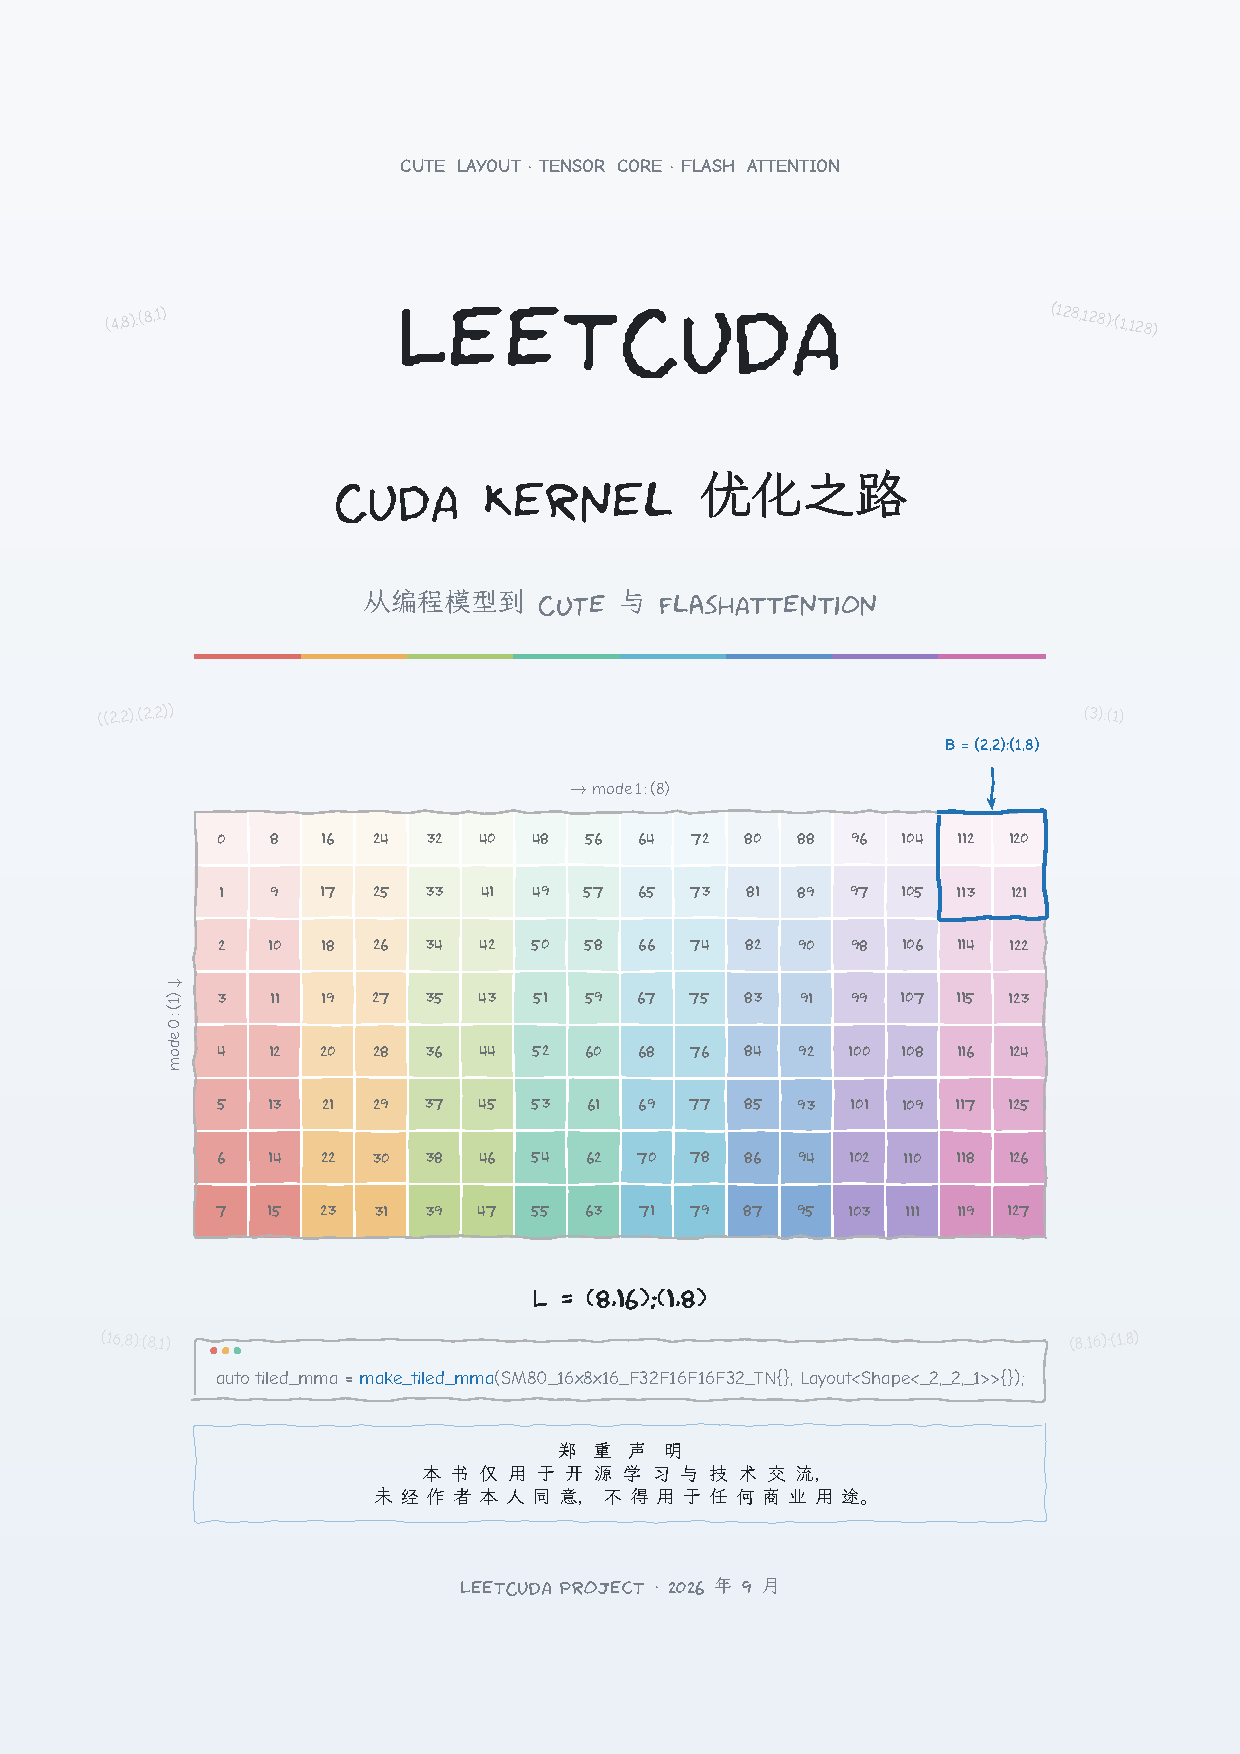
\includegraphics[width=\paperwidth,height=\paperheight]{figures/misc/cover.pdf}}}
\thispagestyle{empty}
\null
\clearpage

% 消除 frontmatter 的奇数开页空页，目录紧跟封面
\begingroup
\let\cleardoublepage\clearpage
\frontmatter
\tableofcontents
\endgroup

% openany 电子书不强制右页起始：否则目录尾(xix)后 \mainmatter 的
% \cleardoublepage 会补一页空白 xx（fancyhdr 沿用目录页眉）。全书统一取消补页。
\let\cleardoublepage\clearpage
\mainmatter

\part{基础篇：编程模型、访存与归约}
% ch00-profiling.tex — 性能分析先于优化：nsys 与 ncu（RFC-C0）
% 工具方法论章：无对应源码区间，无编译宏限定，全 arch 通用
% 本章无 device kernel：book/tests/ 不设 ch00 测试；实战数据引自作者参与的 CUDA kernel 开发 NCU/NSYS 分析记录
\chapter{性能分析先于优化：nsys 与 ncu}\label{ch:00}

\section{本章导读}

在动手写第一个 kernel 之前，本书想先立一条工程信条：\textbf{profile 永远都是
最重要的}。优化 GPU kernel 的正确循环不是「改了跑一下看快没快」，而是
「先测量、再假设、改一处、再测量」。凭直觉的优化是赌博：赢了是运气，输了
连原因都找不到。这一章专门讲两件测量工具——\textbf{Nsight Systems}（nsys，
全局时间线）与 \textbf{Nsight Compute}（ncu，单 kernel 计数器）——的原理、
命令行用法与核心指标的含义，并给出一张「症状 $\to$ 证据 $\to$ 结论 $\to$
对策」的瓶颈判断决策树。

本章不含 kernel（与 ch01 及 Part IV 的原理章 ch20--22 一样，是纯理论/工具章）。没有新代码可讲，但有大量
\textbf{实战教训}：它们全部来自真实的 CUDA kernel 开发记录——寄存器压力、spill、warp stall、Tensor Core 饱和度、
L1/L2 命中率、bank conflict，每一个指标都配一个真实的「指标驱动优化」或
「指标否决优化」案例。后续所有章节的「性能分析」节都默认读者已掌握本章的
工具与词汇表。

\textbf{前置}：无（与 ch01 互为入口，roofline 词汇见 ch01）。
\textbf{源码区间}：无（工具方法论章）。\textbf{编译宏与架构限定}：无。

\section{问题与动机：凭感觉的优化是赌博}

先看三个真实的开发反例，说明「不 profile 就优化」会栽在哪里。

\textbf{反例一：感觉是装载瓶颈，其实是依赖链}。一个 sm\_89 上的 fp8
attention kernel（persist-D 结构）对标业界最快实现慢 28\%（909.4$\mu$s vs
710$\mu$s）。直觉方案是「加深装载流水、砍指令、缩 tile」，全部实测无效；
NCU 的 stall 剖析结果一锤定音：\texttt{math\_\allowbreak{}pipe\_\allowbreak{}throttle} 1.32
主导、\texttt{wait} 0.82、\texttt{long\_\allowbreak{}scoreboard} 仅
0.04——\textbf{装载根本不是瓶颈}，瓶颈是单 CTA 内 softmax$\to$PV 的串行
依赖链，唯一有效的改动是拆链（2 CTA/SM），实测 $-5\%$。

\textbf{反例二：感觉主 kernel 慢，其实差距在别处}。e2e 落后时先盯着主 kernel
跑 ncu，做完整套指标分析才发现主 kernel 已占 e2e 时间 86--92\%、前处理链
已优于对照——一次 nsys 的时间线本可以三分钟得出同样结论，避免在错误的
kernel 上浪费半天 ncu 分析。

\textbf{反例三：感觉融合更快，其实更慢}。把 softmax 的 bias 注入从「分离
kernel」改成「单 pass 融合 + smem tile」，直觉上少一次读写应该更快，实测反而
慢 4.2ms：NCU 显示融合把 LDS（shared load）拉进了 consumer 关键路径，
\texttt{sleeping} stall 从 3.5\% 暴涨到 22.3\%。指标否决了这次「优化」。

三个反例的共同教训：GPU 上的性能瓶颈极少长在直觉指向的地方。成熟的优化
工作流会把它固化成一条硬规则：\textbf{没有 NCU 数据，不改 kernel}；
每条优化结论必须引用具体 metric 数值作为证据。本章就把这套「证据
从哪里来、怎么读」讲透。

\section{工具链总览与顺序方法论}\label{sec:ch00-tools}

\subsection{两个工具回答两个不同的问题}

nsys 与 ncu 的采集原理完全不同：

\begin{itemize}
\item \textbf{nsys（Nsight Systems）}：\textbf{trace} 型。在驱动层记录 API
  调用、kernel launch、内存拷贝、流与事件的时间戳，拼出一张全局时间线。
  它回答「\textbf{时间花在哪}」：哪个 kernel 占比最大、kernel 之间有没有
  空隙（gap）、CPU launch 是否跟不上、多流是否真的在重叠。代价低——不需要
  GPU 性能计数器权限，任何环境都能跑，被测程序几乎不失真。
\item \textbf{ncu（Nsight Compute）}：\textbf{counter replay} 型。要读一个
  kernel 的成百上千个硬件计数器（SM 吞吐、cache 命中、warp stall……），
  而一遍执行采不完这么多计数器，于是 ncu 把 kernel \textbf{回放多遍}，
  每遍采一组；为了数据可比还会锁定时钟。它回答「\textbf{这个 kernel 内部
  慢在哪}」。代价高——单 kernel 深挖、时间被串行化与放大，\textbf{ncu 报告
  里的 kernel 耗时不能当 bench 时间用}。
\end{itemize}

一句话分工：nsys 是体检报告（哪里有病），ncu 是专科检查（病灶细胞级切片）。

\subsection{顺序：先 nsys，后 ncu}

顺序不是习惯问题，是成本问题：

\begin{enumerate}
\item \textbf{nsys 先行}：一次采集拿到全部 kernel 的时间占比排序。如果主
  kernel 占 86\%，那么辅助 kernel 再难看也只有 14\% 的优化上限——先确认
  「该优化谁」，再谈「怎么优化」。nsys 还能立刻暴露三类结构性问题：launch
  gap（CPU 跟不上，一个真实案例 wall-GPU 差 129$\mu$s vs 对照 50$\mu$s，
  病根在 dispatch 而非 kernel）、该并行的流没重叠、意外的 fallback kernel。
\item \textbf{ncu 跟进}：只对 nsys 排出的 Top-1/Top-2 kernel 做
  \texttt{-{}-set full} 深挖，读 roofline、occupancy、stall、memory 各维
  指标，形成假设。
\item \textbf{单变量修改 $\to$ 复测}：每次只改一处，re-profile 后用
  \texttt{-{}-diff} 对照前后指标；无效或负优化立即回退。
\end{enumerate}

反着来的代价见本章开头的反例二：先 ncu 后 nsys，等于对着一个可能不重要的
kernel 做了半天细胞级切片。

\begin{figure}[H]
\centering
\begin{tikzpicture}[
  font=\footnotesize,
  box/.style={draw, rounded corners=2pt, align=center, inner sep=3pt,
    font=\scriptsize, text width=2.2cm, minimum height=1.0cm},
  ar/.style={-{Stealth[length=1.8mm]}, semithick}
]
  \node[box, text width=1.3cm] (e2e) at (0.95, 0) {e2e\\落后};
  \node[box, fill=gray!15] (nsys) at (3.4, 0)
    {nsys 全局时间线\\\texttt{-t cuda} 单域\\kern\_sum 占比排序};
  \node[box] (top) at (6.35, 0)
    {Top-1/2 kernel\\主 kernel 占 86--92\%\\$\to$ 辅助链上限仅 14\%};
  \node[box, fill=gray!40] (ncu) at (9.3, 0)
    {ncu 单 kernel 深挖\\\texttt{-{}-set full}\\\texttt{regex:} 名字前缀};
  \node[box] (judge) at (12.35, 0)
    {指标判读\\（接决策树\\图~\ref{fig:0-1}）};
  \draw[ar] (e2e.east) -- (nsys.west);
  \draw[ar] (nsys.east) -- (top.west);
  \draw[ar] (top.east) -- (ncu.west);
  \draw[ar] (ncu.east) -- (judge.west);
  \node[box, fill=gray!65] (modi) at (12.35, -2.35)
    {单变量修改\\每次只改一处};
  \node[box, fill=gray!65] (diff) at (8.9, -2.35)
    {复测 \texttt{-{}-diff}\\前后指标对照};
  \node[box] (keep) at (5.2, -2.35) {有效 $\to$ 保留};
  \draw[ar] (judge.south) -- (modi.north);
  \draw[ar] (modi.west) -- (diff.east);
  \draw[ar] (diff.west) -- (keep.east)
    node[midway, above, font=\scriptsize] {有效};
  \node[box, dashed] (revert) at (8.9, -4.1)
    {无效 / 负优化\\$\to$ 回退};
  \draw[ar] (diff.south) -- (revert.north)
    node[midway, right, font=\scriptsize] {无效};
  \draw[ar, dashed] (revert.east) -- (14.1, -4.1) -- (14.1, 0) -- (judge.east);
  \node[font=\scriptsize, anchor=west, text=black!60] at (14.25, -2.0)
    {回到判读};
\end{tikzpicture}
\caption{nsys $\to$ ncu $\to$ 单变量修改 $\to$ 复测 \texttt{-{}-diff} 的闭环工作流：nsys 先给全局占比与优化预算（主 kernel 占 86--92\%，辅助链上限仅 14\%，对应 \S\ref{sec:ch00-cases} 例一）；ncu 只深挖 Top-1/2 kernel；每次只改一处，复测后无效立即回退、回到指标判读。泳道灰度：nsys 15\%、ncu 40\%、修改/复测 65\%。}
\label{fig:0-2}
\end{figure}

\section{nsys 命令行实战}\label{sec:ch00-nsys}

\subsection{最小采集}

原则：\textbf{只采需要的域、只采最短的窗口}。对「看 kernel 占比」这个目标，
一条 trace 域 \texttt{-t cuda} 就够，CPU 采样与上下文切换全部关掉，warmup
与 repeat 压到最小：

\begin{lstlisting}[style=console, title={nsys 最小采集（kernel 时间占比场景）}]
nsys profile -t cuda --sample=none --cpuctxsw=none \
  -o .tmp/ch00/report.nsys-rep python bench.py
\end{lstlisting}

\subsection{stats 报表：两个最常用的 report}

采集产物是 \texttt{.nsys-rep}，用 \texttt{nsys stats} 导出统计：

\begin{lstlisting}[style=console, title={nsys stats 两个高频 report}]
nsys stats -r cuda_gpu_kern_sum report.nsys-rep   # per-kernel 时间占比（最常用）
nsys stats -r cuda_gpu_trace   report.nsys-rep   # per-launch 时间线（看 gap/流重叠）
\end{lstlisting}

\texttt{cuda\_\allowbreak{}gpu\_\allowbreak{}kern\_\allowbreak{}sum} 按 kernel 聚合总时长与占比，直接给出「该优化
谁」的答案；\texttt{cuda\_\allowbreak{}gpu\_\allowbreak{}trace} 逐 launch 列时间戳，用来看相邻 kernel
间的空隙与多流 overlap。首次对旧 report 运行时报
\texttt{Existing SQLite export found} 时，加 \texttt{-{}-force-export=\allowbreak{}true}
强制重新导出。

\subsection{体积控制：一次 500GB 事故}

nsys 的中间数据默认写到 \texttt{/\allowbreak{}tmp/\allowbreak{}nvidia/\allowbreak{}nsight\_\allowbreak{}systems}，体积 $\approx$
单事件字节数 $\times$ 事件数，而事件数随时长线性增长。对大模型推理（多模型链、大 seqlen、多次 repeat）无脑
全量采集，曾把 \texttt{/tmp} 写到 \textbf{500GiB+} 直到磁盘写满系统卡死
（真实事故，2026-09）。
三条铁律：

\begin{enumerate}
\item \textbf{输出与临时文件落项目目录}：显式设 \texttt{TMPDIR} 指向项目
  \texttt{.tmp/} 下的目录并用 \texttt{-o} 指定输出，事后清理。注意 TMPDIR
  路径要短——过长的路径会撑爆 Unix domain socket 的 107 字节上限（Ray 的
  plasma store 直接构造失败）。
\item \textbf{禁止对大模型 e2e 无脑全量采}：repeat 降到 0--1，单域
  \texttt{-t cuda}，关采样。
\item \textbf{优先 torch.profiler}：只想看 kernel 时间表时，
  \texttt{torch.\allowbreak{}profiler} 输出 chrome trace 落在 \texttt{.tmp/}，零外部临时
  文件风险；nsys 只在必须看时间线/同步事件时出场。
\end{enumerate}

\subsection{窗口化采集：cudaProfilerApi}

只想采推理中的一小段（比如 50 个 denoise step 中的 1 步）时，用
\texttt{-{}-capture-range=\allowbreak{}cuda\allowbreak{}Profiler\allowbreak{}Api} 配合代码里的开关，把采集窗口钉在
目标区间：

\begin{lstlisting}[style=console, title={窗口化采集（Python 侧）}]
nsys profile -t cuda --capture-range=cudaProfilerApi \
  --sample=none --cpuctxsw=none -o .tmp/ch00/win python bench.py
# bench.py 内：
#   torch.cuda.profiler.start()   # 窗口开始
#   ... 目标 step ...
#   torch.cuda.profiler.stop()    # 窗口结束
\end{lstlisting}

\section{ncu 命令行实战}\label{sec:ch00-ncu}

\subsection{基础采集与 section}

\begin{lstlisting}[style=console, title={ncu 全量采集与 CSV 导出}]
ncu --set full -o .tmp/ch00/report_v1 --target-processes all ./kernel_app
ncu --import .tmp/ch00/report_v1.ncu-rep --page raw --csv > report_v1.csv
\end{lstlisting}

\texttt{-{}-set full} 采全部 section（roofline、occupancy、warp state、
memory workload、instruction mix……），单 kernel 回放多遍、耗时可观；快速
确认可用默认 basic set。交互式 \texttt{ncu-ui} 看报告，命令行用
\texttt{-{}-page details}（rule-based 汇总）或 \texttt{-{}-page raw}（原始
metric，见下）。

\subsection{-{}-kernel-name 必须用 regex: 前缀}

C++ 模板 kernel 的完整名带一长串后缀（如
\texttt{persist\_\allowbreak{}d\_\allowbreak{}ws\_\allowbreak{}fwd\_\allowbreak{}cute\_\allowbreak{}fp8\_\allowbreak{}sm120}，实际实例化名比这更长）。
\texttt{-{}-kernel-name} 默认\textbf{精确匹配}，拿「名字的前缀」去匹配会报
\texttt{No kernels were profiled} 且生成空 report。必须加 \texttt{regex:}
前缀走部分匹配：

\begin{lstlisting}[style=console, title={kernel 名过滤：regex 前缀}]
ncu --set full -o rep --kernel-name regex:persist_d_ws_fwd_cute_fp8 \
  --target-processes all ./app     # OK：部分匹配
ncu --kernel-name persist_d_ws_fwd_cute_fp8_sm120 ...  # 错：精确匹配，0 命中
\end{lstlisting}

\subsection{-{}-page raw 提取原始 metric}

ncu 的 \texttt{-{}-csv} 默认输出是 \textbf{rule-based} 的 section 汇总（按
诊断规则组织），不是逐个原始计数器。要拿具体 stall reason 的数值，必须走
\texttt{-{}-page raw}。raw 输出里每个 metric 是「名字行 + 单位行 + 数值行」
的多行结构，用 \texttt{grep -A3} 抓：

\begin{lstlisting}[style=console, title={从 raw page 提取 stall 指标}]
ncu --import rep.ncu-rep --page raw 2>&1 | \
  grep -A3 "warps_issue_stalled_\(wait\|math_pipe_throttle\|sleeping\)"
\end{lstlisting}

\subsection{权限限制与同架构代理 GPU}

读性能计数器需要驱动授权。容器/云主机上常见
\texttt{/proc/\allowbreak{}driver/\allowbreak{}nvidia/\allowbreak{}params} 里
\texttt{Rm\allowbreak{}Profiling\allowbreak{}Admin\allowbreak{}Only} 标志为 1，
此时 \texttt{-{}-set full} 直接报 \texttt{ERR\_\allowbreak{}NVGPUCTRPERM}，且容器内无法
reload 驱动。可行解法是\textbf{同架构代理}：找一块相同微架构的本地 GPU 跑
ncu——例如用本地 RTX PRO 5000（sm\_120a）代理远端 RTX 5090（sm\_120）。
stall reasons、指令 mix、occupancy 这类\textbf{架构级}结论可以迁移，绝对
性能数字（SM 数、频率、L2 容量）不可迁移；ncu 验证完架构结论后，回目标
硬件跑 timing bench 收数。

\subsection{replay 的干扰与 A/B 纪律}

ncu 锁频 + 多遍回放 + 串行执行，因此\textbf{报告内耗时只用于相对比较}。
做优化 A/B 时回到真实 bench，并遵守两条纪律：

\begin{itemize}
\item \textbf{校验公共参照}：许多 bench 会同时输出被测实现与公共参照
  （如 PyTorch SDPA）两组时间；对比前先核对两轮参照是否吻合（$\pm$1\%）。
  被 GPU 级干扰（并发进程/时钟态）污染的一轮，两者会\textbf{同比例膨胀}
  （实测约 $2\times$），直接对比会得出「$-50\%$ 全面加速」这种物理上不可能
  的假结论。
\item \textbf{min-of-N 口径}：单轮抖动大的实现（如 tma 变体）取 N 次最小值
  对比；归因 race 类问题必须 stash $\to$ 重建 $\to$ 同 probe 的 HEAD 对照，
  单次「好结果」不可信。
\end{itemize}

\section{核心指标字典}\label{sec:ch00-metrics}

以下每个指标按「含义 / 怎么读 / 异常意味着什么 / 对策」展开。数值口径以
sm\_120 上的实测为参照。

\subsection{SpeedOfLight：SM\% 与 MEM\%（roofline 定位）}

\texttt{sm\_\allowbreak{}\_\allowbreak{}throughput}（SM\%）与 \texttt{gpu\_\allowbreak{}\_\allowbreak{}compute\_\allowbreak{}memory\_\allowbreak{}throughput}
（MEM\%）分别是计算管线与内存管线的峰值利用率，是 NCU 报告的第一行。
两者把 kernel 放上 ch01 的 roofline：SM\% 高 MEM\% 低是 compute-bound，
反之 memory-bound；\textbf{双低}（如 SM/MEM 都在 30\% 附近）则是
latency-bound——管线都没喂满，问题在并行度或依赖链，这是 roofline 图上
看不出的第三态，必须回到 stall 指标找证据。

\subsection{Occupancy：理论、达到与三类限制源}

区分两个数：\textbf{理论 occupancy}（kernel 资源能驻留多少 warp，受三类
限制源钳制——寄存器、smem、block/warp 上限）与\textbf{达到 occupancy}
（\texttt{sm\_\allowbreak{}\_\allowbreak{}warps\_\allowbreak{}active}，实际运行均值，受 tail effect 与负载不均
拖累）。NCU 的 Occupancy section 会明确指出 \texttt{launch\_\allowbreak{}\_\allowbreak{}occupancy\_\allowbreak{}limit\_\allowbreak{}registers} /
\texttt{\_\allowbreak{}\_\allowbreak{}shared\_\allowbreak{}mem} / \texttt{\_\_blocks} 哪个是当前限制源。一个
fp8 attention kernel 的实例：REG:255 直接把 \texttt{Block Limit Registers} 压到 1——
1 CTA/SM、12 warps（4 producer + 8 consumer，共 384 线程），理论 occupancy
25\%（12/48），此时想提并行度只有降寄存器或换结构
（见 \S\ref{sec:ch00-cases} 例二）。注意 ch01 的告诫：occupancy 是手段不是
KPI，GEMM 类 kernel 用大 tile + 低 occupancy + 高 ILP 换性能是常态。

\begin{figure}[H]
\centering
\begin{tikzpicture}[font=\footnotesize,
  lab/.style={font=\scriptsize, inner sep=1pt}]
  \draw[-{Stealth[length=1.8mm]}] (0, 0) -- (13.3, 0);
  \draw[-{Stealth[length=1.8mm]}] (0, 0) -- (0, 6.75);
  \foreach \x/\t in {1.44/32, 2.88/64, 5.76/128, 8.64/192, 11.52/256}
    {
      \draw (\x, 0) -- (\x, -0.08);
      \node[lab, anchor=north] at (\x, -0.1) {\t};
    }
  \foreach \y/\t in {0.92/8, 1.84/16, 2.76/24, 3.68/32, 4.60/40}
    {
      \draw (0, \y) -- (-0.08, \y);
      \node[lab, anchor=east] at (-0.1, \y) {\t};
    }
  \draw (0, 5.52) -- (-0.08, 5.52);
  \node[lab, anchor=east, font=\scriptsize\bfseries] at (-0.1, 5.52) {48};
  \draw[black!30, semithick] plot[smooth] coordinates
    {(1.80,5.89) (2.16,4.91) (2.52,4.21) (2.88,3.68) (3.24,3.27) (3.60,2.94)
     (4.32,2.45) (5.04,2.10) (5.76,1.84) (7.20,1.47) (8.64,1.23) (10.08,1.05)
     (11.52,0.92)};
  \draw[black!45, semithick] (0.3, 3.68) -- (7.9, 3.68);
  \draw[black!60, semithick] (0.3, 5.52) -- (11.8, 5.52);
  \draw[very thick]
    (0.3,3.68) -- (2.88,3.68) -- (2.88,2.76) -- (3.83,2.76) -- (3.83,1.84)
    -- (5.76,1.84) -- (5.76,0.92) -- (11.52,0.92);
  \node[lab, anchor=south west] at (4.7, 5.72) {block/warp 槽位上限：48 warps};
  \node[lab, anchor=south west, align=left] at (3.3, 3.9)
    {smem 约束（示例：\\smem/block=32KB，T=256）\\$\to$ 上限 32 warps};
  \node[lab, anchor=west, align=left] at (11.68, 0.92)
    {寄存器约束\\$65536/(32r)$};
  \node[lab, anchor=west, align=left] at (11.68, 2.35)
    {粗黑阶梯 = min\\（整 block 量化，\\T=256 $\to$ 8 warps/级）};
  \fill (11.48, 1.38) circle (0.07);
  \draw[black!60, thin] (9.8, 4.1) -- (11.42, 1.47);
  \node[lab, anchor=north west, align=left] at (8.45, 5.25)
    {实测点（WS 结构，例二）：\\consumer REG 255 / producer 32\\
     1 CTA/SM = 12 warps（384T）\\理论 occupancy 25\%（12/48）};
  \node[lab, anchor=north] at (6.65, -0.42) {每线程寄存器数 $r$（regs/thread）};
  \node[lab, rotate=90, anchor=south] at (-0.95, 3.3) {可驻留 warp/SM};
\end{tikzpicture}
\caption{理论 occupancy 的三限制源取 min（sm\_120，48 warp 槽位口径）：寄存器约束 $65536/(32r)$（warp 粒度简化）随每线程寄存器数 $r$ 下降；smem 与槽位为水平约束（示例：smem/block=32KB、T=256 $\to$ 32 warps）。粗黑阶梯为按整 block（T=256，8 warps/block）量化的 min 包络；实测点为 WS 结构（producer 32 / consumer 232 regs）1 CTA/SM = 12 warps（384T），理论 occupancy 25\%（12/48）。}
\label{fig:0-3}
\end{figure}

\subsection{寄存器与 spill：255 墙}

\texttt{launch\_\allowbreak{}\_\allowbreak{}registers\_\allowbreak{}per\_\allowbreak{}thread} 给出每线程寄存器数，硬上限
\textbf{255}（每线程）。超限时编译器把变量溢出到 local memory（SASS 里表现为
\texttt{LDL}/\texttt{STL} 指令，NCU 里看
\texttt{l1tex\_\allowbreak{}\_\allowbreak{}t\_\allowbreak{}bytes\_\allowbreak{}pipe\_\allowbreak{}lsu\_\allowbreak{}mem\_\allowbreak{}\allowbreak{}local\_\allowbreak{}op\_\allowbreak{}\_\allowbreak{}ld/\allowbreak{}st.sum} 是否非零）。
编译期排查用 \texttt{-{}-ptxas-options=\allowbreak{}-v} 与
\texttt{cuobjdump -{}-dump-resource-usage} 的 STACK 字节。两个实战要点：

\begin{itemize}
\item \textbf{spill 的代价主要不是流量}。一个 fp4 attention kernel 在
  D=512 时 spill 总量 234MB，但 local 流量仅 12.8GB/s——带宽上无关痛痒，真正的代价
  是\textbf{延迟暴露}：8 warps/SM 意味着每 scheduler 只有 2 个 warp 可切换，
  LDL 的几百 cycle 延迟藏不住，同时指令数也变多。
\item \textbf{寄存器预算可以算出来}。attention 的 O 累加器每线程占
  $k_{Br}\cdot D/256$ 个 f32 寄存器（M8N1 布局，$256=32$ lanes $\times 8$
  个 warp——consumer 全部 256 线程）；$k_{Br}{=}128$ 时为
  $D/2$，D=512 要 256 个——\textbf{撞穿 255 墙}。这正是大 D 必须换
  M4N2 atom（列拆给两个 warp，每线程 $D/4$）的数学来源（ch19）。
\end{itemize}

\subsection{Warp State：stall reasons，好 stall 与坏 stall}

warp 每个周期若不能发射，必有一个「停滞原因」。sm\_120 上的口径是
\texttt{smsp\_\allowbreak{}average\_\allowbreak{}warps\_\allowbreak{}issue\_\allowbreak{}stalled\_\allowbreak{}*\_\allowbreak{}per\_\allowbreak{}issue\_\allowbreak{}active.\allowbreak{}ratio}
——每个发射周期停在该原因上的平均 warp 数。表~\ref{tab:00-stall}
是实战中最常读的八项：

\begin{table}[htbp]
\centering
\caption{warp stall 指标字典（sm\_120 实测口径）}
\label{tab:00-stall}
\begin{tabular}{lp{5.2cm}p{5.6cm}}
\toprule
指标后缀 & 含义 & 高值时怎么办 \\
\midrule
\texttt{wait} & 固定延迟依赖（寄存器/ALU 结果未就绪） & 依赖链问题：拆链、增并行 warp、重排指令；attention 的 softmax$\to$PV 串行链是典型来源 \\
\texttt{long\_\allowbreak{}scoreboard} & 等 gmem/TMA 数据 & 装载不足：\texttt{cp.async}/TMA、加深 stage、prefetch \\
\texttt{short\_\allowbreak{}scoreboard} & 等 smem（MIO 队列） & LDS 链太长：swizzle 布局、减少 smem 往返 \\
\texttt{math\_\allowbreak{}pipe\_\allowbreak{}throttle} & 数学管线排队满 & \textbf{好信号}：计算饱和。保持或进一步减 FLOPs \\
\texttt{sleeping} & warp 休眠（mbarrier 退避） & \textbf{纯浪费}：producer/consumer 失衡或空转自旋，查 WS 结构 \\
\texttt{barrier} & 等显式栅栏 & 同步过频：减少 \texttt{\_\allowbreak{}\_\allowbreak{}syncthreads} 点、缩 block \\
\texttt{not\_\allowbreak{}selected} & 就绪但调度器选了别人 & \textbf{健康}：有冗余并行度可隐藏延迟 \\
\texttt{selected} & 正在发射（非停滞） & 基线，越大越好 \\
\bottomrule
\end{tabular}
\end{table}

读 stall 剖析结果的关键是\textbf{分好坏}：\texttt{math\_\allowbreak{}pipe\_\allowbreak{}throttle} 与
\texttt{not\_\allowbreak{}selected} 高说明机器在干活；\texttt{sleeping} 高几乎总是结构
问题；\texttt{wait} 与 \texttt{long\_\allowbreak{}scoreboard} 的\textbf{相对大小}直接
区分「依赖链受限」与「装载受限」——例见 \S\ref{sec:ch00-cases} 例三。

\subsection{Memory Workload：L1/L2/DRAM 分层归因}

三层各看两个数——命中率与吞吐：

\begin{itemize}
\item \textbf{L1/TEX}：\texttt{l1tex\_\allowbreak{}\_\allowbreak{}t\_\allowbreak{}sector\_\allowbreak{}hit\_\allowbreak{}rate.pct}。低于
  20\% 且数据本该复用时，考虑 tiling 进 smem 或改访问模式。注意 smem 与 L1
  \textbf{共池}（GB202 实测每多占 16KB smem，kernel 约慢 4--5$\mu$s），
  「多分 smem」不是免费的。
\item \textbf{L2}：\texttt{lts\_\allowbreak{}\_\allowbreak{}t\_\allowbreak{}sector\_\allowbreak{}hit\_\allowbreak{}rate.\allowbreak{}pct}。大 GEMM 上低
  命中可用 CTA swizzle / StreamK 提数据局部性；推理场景 K/V 重复读高命中
  是常态。
\item \textbf{DRAM}：\texttt{dram\_\allowbreak{}\_\allowbreak{}throughput}（峰值百分比）。贴满
  （$>$70\%）说明带宽墙已到，优化方向只剩减流量（混合精度、融合、去
  物化）。一条量化前处理链实测贴到饱和带宽 1.04TB/s（约为理论峰值
  1344GB/s 的 77\%）——此时「融合省 launch」已无杠杆，只有减流量才有，这个
  判断直接由 DRAM 指标给出。
\item \textbf{load/store 与合并访问}：global load 的每请求扇区数
  （\texttt{l1tex} 前缀的
  \texttt{average\_\allowbreak{}t\_\allowbreak{}sectors\_\allowbreak{}\_\allowbreak{}per\_\allowbreak{}request\_\allowbreak{}\allowbreak{}...} 系列指标）
  衡量合并访问质量——32-bit 连续访问的理想值是 4（一个 warp 的 128B 恰好
  4 个 32B sector）；明显超标说明访存发散，流量被放大，对策是内维连续、
  向量化（\texttt{float4} 128-bit 访存，ch03）与 AoS$\to$SoA。IO 压力的
  完整画像由三个正交维度拼出：\textbf{吞吐}（哪层饱和）、\textbf{命中率}
  （数据该由哪层负责）、\textbf{合并度}（流量有没有被访问模式放大）。
\end{itemize}

分层归因顺序：DRAM 饱和先看是不是 L2 miss 推的（L2 hit 低 + DRAM 高 =
工作集溢出），L2 高命中但 L1 低命中 = smem/L1 复用不足。IO 压力的「层」
定位错了，对策就全错。

\subsection{bank conflict 与 smem 指标}

\texttt{l1tex\_\allowbreak{}\_\allowbreak{}data\_\allowbreak{}bank\_\allowbreak{}conflicts\_\allowbreak{}pipe\_\allowbreak{}lsu\_\allowbreak{}mem\_\allowbreak{}\_\allowbreak{}shared\_\allowbreak{}op\_\allowbreak{}ld/\allowbreak{}st.sum}
直接数冲突次数（ch12 表 12-1 的数据来源）。判读要点：\textbf{先看占比再
动手}——曾有一个「消除 O 写回 bank conflict」的优化立项，NCU 一查
ld conflict 仅 0.39\%，且 MUFU 等待被 MMA 掩盖，整个方向当场否决。
冲突计数要换算成「每 warp 每 cycle 的额外重放」才有体感，绝对数大不等于
值得修。

\subsection{指令 mix 与 tensor pipe 利用率}

各执行管线的活跃占比（\texttt{pipe\_fma} / \texttt{pipe\_alu} /
\texttt{pipe\_lsu} / \texttt{pipe\_tensor}）回答「指令都花在哪了」。
对本书 Part II--IV 的主线而言，\textbf{tensor pipe 利用率就是 Tensor Core
饱和度}：fp16 GEMM 类 kernel 若 \texttt{pipe\_fma} 高而 \texttt{pipe\_tensor}
低，说明还在用 CUDA Core 算乘加，应该换 MMA 指令（ch10--11 的主题）。
一个 fp8 kernel 的实例：tensor pipe 从 49\% 提到 59.5\% 的那次优化，
判据正是「\texttt{math\_\allowbreak{}pipe\_\allowbreak{}throttle} 降了、tensor pipe 升了」——两条
指标共同确认依赖链被拆开、Tensor Core 被喂得更满。

\section{瓶颈判断决策树}\label{sec:ch00-tree}

把上述指标串成一条判断流程（数值阈值为工程经验值，非硬边界）：

\begin{figure}[H]
\centering
\begin{tikzpicture}[
  font=\footnotesize,
  box/.style={draw, rounded corners=2pt, align=center, inner sep=3pt,
    text width=2.6cm, minimum height=8mm},
  dec/.style={box, draw=tkBlue, fill=tkFillBlue},
  memb/.style={box, draw=tkOrange, fill=tkFillOrange},
  cpub/.style={box, draw=tkPurple, fill=tkFillPurple},
  latb/.style={box, draw=tkRed, fill=tkFillRed},
  balb/.style={box, draw=tkGreen, fill=tkFillGreen},
  det/.style={draw, align=left, inner sep=3pt, font=\scriptsize,
    text width=5.1cm, fill=white},
  detm/.style={det, draw=tkOrange!85},
  detc/.style={det, draw=tkPurple!85},
  detl/.style={det, draw=tkRed!70},
  badge/.style={circle, draw=black!70, fill=white, inner sep=0pt,
    minimum size=3.6mm, font=\scriptsize\bfseries, anchor=south east},
  ar/.style={-{Stealth[length=1.8mm]}, semithick},
  arm/.style={ar, draw=tkOrange},
  arc/.style={ar, draw=tkPurple},
  arl/.style={ar, draw=tkRed!85}
]
  \node[dec] (root) at (0, 0.55) {读 SOL\\（SM\% / MEM\%）};
  \node[badge] at (root.north west) {1};
  \node[memb] (mcond) at (3.8, 4.2) {MEM\% $\gg$ SM\%\\（差 $>$20）};
  \node[memb] (mver) at (7.9, 4.2) {memory-bound\\分层归因};
  \node[badge] at (mver.north west) {4};
  \node[detm] (md1) at (12.9, 5.4) {DRAM $>$70\% $\to$ 带宽墙\\对策：减流量（融合 / 低精度 / 去物化）};
  \node[detm] (md2) at (12.9, 4.2) {L2 hit $<$50\% 且 DRAM $>$40\%\\$\to$ 工作集 / L2 局部性（CTA swizzle）};
  \node[detm] (md3) at (12.9, 3.0) {L1 hit $<$20\% 而 L2 高\\$\to$ smem tiling / 复用不足};
  \node[cpub] (ccond) at (3.8, 1.2) {SM\% $\gg$ MEM\%};
  \node[cpub] (cver) at (7.9, 1.2) {compute-bound\\查饱和质量};
  \node[badge] at (cver.north west) {5};
  \node[detc] (cd1) at (12.9, 1.8) {tensor pipe 高 = 健康\\$\to$ 减 FLOPs 或更低精度};
  \node[detc] (cd2) at (12.9, 0.6) {pipe\_fma / alu 高、tensor 低\\$\to$ 该上 MMA 指令（ch10--11）};
  \node[latb] (lcond) at (3.8, -1.8) {双低\\（都 $<$40）};
  \node[latb] (lver) at (7.9, -1.8) {latency-bound\\stall 前二名分流};
  \node[badge] at (lver.north west) {2};
  \node[detl] (ld1) at (12.9, -0.6) {\texttt{wait} / \texttt{math\_pipe\_throttle} 主导\\$\to$ 拆链、增并行 warp};
  \node[detl] (ld2) at (12.9, -1.8) {\texttt{long\_scoreboard} 主导\\$\to$ 异步装载（TMA / cp.async）};
  \node[detl] (ld3) at (12.9, -3.0) {\texttt{sleeping} / \texttt{barrier} 主导\\$\to$ 重排 producer/consumer（WS）};
  \node[detl, dashed, text width=5.5cm] (occ) at (7.9, -4.55) {先查 occupancy 限制源：\\limiter = regs/smem $\to$ 先解资源\\（缩 tile、降 stage、launch\_bounds）\\「增并行 warp」以有 warp 可增为前提};
  \node[badge] at (occ.north west) {3};
  \node[balb] (dcond) at (3.8, -6.15) {双高\\（都 $>$60）};
  \node[balb] (dver) at (7.9, -6.15) {接近平衡上限\\$\to$ 停止优化};
  \draw[ar, draw=tkBlue] (root.east) -- (mcond.west);
  \draw[ar, draw=tkBlue] (root.east) -- (ccond.west);
  \draw[ar, draw=tkBlue] (root.east) -- (lcond.west);
  \draw[ar, draw=tkBlue] (root.east) -- (dcond.west);
  \draw[arm] (mcond) -- (mver);
  \draw[arc] (ccond) -- (cver);
  \draw[arl] (lcond) -- (lver);
  \draw[ar, draw=tkGreen] (dcond) -- (dver);
  \draw[arm] (mver.east) -- (md1.west);
  \draw[arm] (mver.east) -- (md2.west);
  \draw[arm] (mver.east) -- (md3.west);
  \draw[arc] (cver.east) -- (cd1.west);
  \draw[arc] (cver.east) -- (cd2.west);
  \draw[arl] (lver.east) -- (ld1.west);
  \draw[arl] (lver.east) -- (ld2.west);
  \draw[arl] (lver.east) -- (ld3.west);
  \draw[arl, dashed] (lver.south) -- (occ.north);
\end{tikzpicture}
\caption{瓶颈判断决策树：先读 SOL（SM\%/MEM\%）四分流——蓝为入口判断，橙为 memory-bound 链，紫为 compute-bound 链，红为 latency-bound 链，绿为双高（停止优化）；对策框白底、边框沿用所属分支色。节点角标 1--5 对应正文 enumerate 步骤（阈值为工程经验值）。}
\label{fig:0-1}
\end{figure}

\begin{enumerate}
\item \textbf{先看 SOL}：MEM\% $\gg$ SM\%（差 $>$20）$\to$ memory-bound，
  进第 4 步；SM\% $\gg$ MEM\% $\to$ compute-bound，进第 5 步；\textbf{双低}
  （都 $<$40）$\to$ latency/依赖链问题，进第 2 步；双高（都 $>$60）$\to$
  已接近平衡上限，停止优化。
\item \textbf{latency-bound 分流}（看 stall 前二名）：\texttt{wait} 或
  \texttt{math\_\allowbreak{}pipe\_\allowbreak{}throttle} 主导 $\to$ 依赖链/发射受限，对策是拆链
  （拆 CTA、拆 warp 分工）或增并行 warp；\texttt{long\_\allowbreak{}scoreboard} 主导
  $\to$ 数据供给不足，对策是异步装载（\texttt{cp.async}/TMA）与加深流水；
  \texttt{sleeping}/\texttt{barrier} 主导 $\to$ 同步结构问题，对策是重排
  producer/consumer 与栅栏。
\item \textbf{查 occupancy 是否是限制源}：若 achieved 低且 limiter 是
  registers/smem，先解决资源（缩 tile、降 stage、\texttt{\_\allowbreak{}\_\allowbreak{}launch\_\allowbreak{}bounds\_\allowbreak{}}），
  因为第 2 步的「增并行 warp」以有 warp 可增为前提。
\item \textbf{memory-bound 分层}：DRAM $>$70\% $\to$ 带宽墙，减流量；
  L2 hit $<$50\% 且 DRAM $>$40\% $\to$ 工作集/L2 局部性问题；L1 hit $<$20\%
  而 L2 高 $\to$ smem tiling/复用不足。顺带查 coalescing 与 bank conflict。
\item \textbf{compute-bound 查饱和质量}：tensor pipe 高 = 健康，优化转向
  减 FLOPs 或换更低精度；tensor pipe 低而 fma/alu 高 = 该上 MMA；指令数
  本身异常大时查发散与编译器胶水指令。
\end{enumerate}

\begin{table}[htbp]
\centering
\caption{症状 $\to$ 证据 $\to$ 结论 $\to$ 对策速查}
\label{tab:00-tree}
\begin{tabular}{p{3.4cm}p{4.2cm}p{2.6cm}p{4.4cm}}
\toprule
症状 & 指标证据 & 结论 & 对策 \\
\midrule
e2e 慢但不知谁慢 & nsys kern\_sum 占比 & 定位目标 kernel & 只对 Top-1/2 跑 ncu \\
kernel 慢、带宽没吃满 & MEM\%$\le$40，wait/mpt 主导 & 依赖链受限 & 拆链、2 CTA/SM、增并行 warp \\
装载等数据 & long\_scoreboard 高 & 供给不足 & TMA/cp.async、加深 stage \\
并行度上不去 & occupancy 低 + limiter=regs & 寄存器墙 & 缩 tile、M4N2 拆列、launch\_bounds \\
local ld/st 非零 & LDL/STL、local bytes & spill & 降每线程状态、查 255 墙 \\
空转严重 & sleeping 高 & WS 失衡 & 重排 producer/consumer \\
带宽贴顶 & DRAM $>$70\% & 带宽墙 & 减流量：融合/低精度/去物化 \\
smem 访问慢 & bank conflicts 高 & 冲突重放 & swizzle/pad（ch12） \\
TC 没用上 & pipe\_tensor 低 & CUDA Core 算矩阵 & 换 mma/wgmma 指令 \\
\bottomrule
\end{tabular}
\end{table}

\section{实战三例：占比、寄存器与 stall}\label{sec:ch00-cases}

\subsection{例一：nsys 先行——占比决定优化预算}

场景：一个 fp8/fp4 量化 attention 库的 e2e（含量化前处理链）对标
业界实现。e2e 一度落后，最初的直觉是「辅助链 kernel 太多（每 call
约 13 个）应该融合成一个 Mega Kernel」。先用全局视角（nsys + 每 kernel
带宽核算）确认：大 N 场景\textbf{主 kernel 占 e2e 时间 86--92\%}，而 aux
链每个 kernel 都已贴实测饱和带宽 1.04TB/s——融合只能省 launch 不能减流量，
大 N wall 差实测 $<$0.2\%，方向证伪；真正的杠杆在主 kernel 与引擎层
overlap。\textbf{方法论}：占比数据先给「优化预算上限」（14\% 的池子里抠
不出 30\% 的收益），带宽核算再判「这个池子还抠不抠得动」。

\subsection{例二：寄存器压力——255 墙、spill 与 setmaxnreg 的取舍}

场景：fp8 persist-D kernel 采用 warp specialization（WS）：1 个 producer
warp group（128T，专职 TMA）+ 1 个 consumer（256T，全计算），用
\texttt{setmaxnreg} 把寄存器从 producer（32 个）再分配给 consumer（232 个）。
寄存器压力的证据链分三层：

\begin{itemize}
\item \textbf{静态}：\texttt{cuobjdump -{}-dump-resource-usage}（D=768，
  sm\_120f）——fp8 split\_d REG:255 + STACK 1104--1944B（重 spill）；fp8
  m4n2 REG:255 + STACK 0--264B（几乎无 spill）；fp16 split\_d REG:196--254
  + STACK 约 1536B。STACK 字节就是溢出到 local 的体积。
\item \textbf{动态}：NCU 确认 \texttt{Block Limit Registers=1}（REG:255 的
  直接后果），理论 occupancy 25\%（12 warps/48）且 smem 守卫恒空转——限制源唯一。
\item \textbf{取舍}：consumer 想要更多寄存器（\texttt{setmaxnreg} 上限
  232，实测 224--232 区间性能平坦），但 O 累加器 $D/2$（M8N1）在 D=512 时
  要 256 个——\textbf{撞穿 255 墙}，于是 split-D 的 WS 变体被整体禁用，
  大 D 改走 M4N2 把每线程压力降到 $D/4$。这是「寄存器文件利用率 vs
  occupancy vs 算法结构」三方权衡的标准案例：不是把寄存器降下来就赢，
  而是选一个让 tile、并行度与 spill 同时可接受的工作点。
\end{itemize}

（注意 \texttt{setmaxnreg} 在 sm\_120a 上会被 ptxas C7506 静默忽略，
必须用 sm\_120f 构建，见 ch14。）

\subsection{例三：stall 证据链——好 stall 与坏 stall 的判读}

场景：sm\_89 fp8 persist-D 909.4$\mu$s vs 业界实现 710$\mu$s
（慢 28\%）。NCU 剖析结果：

\begin{itemize}
\item \texttt{math\_\allowbreak{}pipe\_\allowbreak{}throttle} \textbf{1.32}（第一名）、
  \texttt{wait} 0.82、\texttt{long\_\allowbreak{}scoreboard} \textbf{0.04}、tensor
  pipe 49\%、255 regs、1 CTA/SM。
\item 判读：\texttt{long\_\allowbreak{}scoreboard} 近零 $\Rightarrow$ 装载不是瓶颈，
  一切「加深流水/砍指令/缩 tile」无效（后续 6 项实验全部证伪，白跑的原因
  就是没先读这组数）；\texttt{mpt} 高但 tensor pipe 只有 49\% $\Rightarrow$
  管线在排队却没排满 Tensor Core——\textbf{依赖链/发射受限}。
\item 对策与验证：kBr=64 + kBc=64 + 128T（2 CTA/SM 拆链）$\to$ 864$\mu$s
  （$-5\%$），ncu 确认 2 blocks/SM、每线程寄存器降到 250；
  \textbf{指标闭环}：mpt 1.32$\to$0.72、tensor pipe 49\%$\to$59.5\%——
  「排队变短、TC 更饱」与 wall 时间下降互为印证。
\end{itemize}

同族的「坏 stall」案例：bias 注入的 smem tile 版本 \texttt{sleeping} 从
3.5\% 涨到 22.3\%（SASS 采样里 \texttt{SYNCS.\allowbreak{}PHASECHK} mbarrier 自旋占
18\%）——LDS 进了 consumer 关键路径、两级 QK 流水断供，全 warp 自旋等 K，
该版本被指标否决。

\section{常见坑}

\begin{enumerate}
\item \textbf{\texttt{-{}-kernel-name} 精确匹配陷阱}。模板 kernel 名带长
  后缀，前缀匹配报 \texttt{No kernels were profiled} 且生成空 report——
  一律 \texttt{regex:} 前缀。
\item \textbf{ncu harness 与 bench 配置不一致}。profiling 用的配置必须与
  bench 默认逐 flag 对齐；显式传 flag 会覆盖 bench 内部的默认值，实测逐
  flag 传参 vs 全默认可差 13\%，指标分析对象可能根本不是 bench 跑的那个
  kernel 形态。
\item \textbf{A/B 不校验公共参照}。GPU 级干扰让两轮\textbf{同比例膨胀}
  （约 $2\times$），对比出假加速。先核对 bench 输出里的 SDPA 参照时间
  （$\pm$1\% 内）再谈结论；抖动大的实现用 min-of-N。
\item \textbf{把 section 输出当 raw metric}。\texttt{-{}-csv} 默认输出是
  rule-based 汇总；要具体计数器数值必须 \texttt{-{}-page raw}（配合
  \texttt{grep -A3} 抓多行结构）。
\item \textbf{拿 ncu 的耗时报性能}。replay 多遍 + 锁频 + 串行化，报告内
  时间只做相对比较；性能数字一律回真实 bench 采。
\item \textbf{不标性能口径}。写结论必须标注 GPU 型号/架构/日期（PRO 5000
  sm\_120a 与 5090 sm\_120 的架构级结论可互证，绝对数字不可）；fallback
  也要查——小 seqlen（$<$512）时库可能自动 fallback 到 PyTorch SDPA，profile
  到的根本不是目标 kernel。
\item \textbf{nsys 全量采集撑爆磁盘}。大模型 e2e 无限制采集曾写爆
  \texttt{/tmp}（500GiB+）。TMPDIR 落项目目录、单域、最小 repeat、事后必清
  （\S\ref{sec:ch00-nsys}）。
\end{enumerate}

\section{小结}

本章没有写一行 kernel，却给出了全书其余 26 章共同的工作节奏：
\textbf{nsys 定位（谁慢）$\to$ ncu 定性（为什么慢）$\to$ 单变量修改 $\to$
复测 diff $\to$ 指标闭环}。指标字典里最值得带走的三句话：SOL 双低不是
「没病」而是 latency-bound，答案在 stall 剖析结果里；stall 分好坏，
\texttt{math\_\allowbreak{}pipe\_\allowbreak{}throttle} 高是 Tensor Core 喂满的勋章，\texttt{sleeping}
高是结构问题的警报；寄存器 255 墙、spill 与 occupancy 是同一份预算的三种
花法，读数时要一起读。工具路径：ncu/nsys 随 CUDA Toolkit 安装（通常在
\texttt{/\allowbreak{}usr/\allowbreak{}local/\allowbreak{}cuda/\allowbreak{}bin}），不在 PATH 时用绝对路径调用。

\section*{延伸阅读}
\begin{itemize}
\item NVIDIA Nsight Systems 文档：
  \href{https://developer.nvidia.com/nsight-systems}{developer.nvidia.com/nsight-systems}
\item NVIDIA Nsight Compute 文档（含 Profiling Guide 的完整指标索引）：
  \href{https://developer.nvidia.com/nsight-compute}{developer.nvidia.com/nsight-compute}
\item 本书各章「性能分析」节：ch09--14（GEMM/TMA/WS 的指标判读）、ch12
  （bank conflict 计数器实战）、ch19（大 D 寄存器压力模型）、ch01
  （roofline 与 occupancy 的理论侧）。
\end{itemize}

% ch01-arch-roofline.tex — 骨架（RFC-0.3），撰写任务见 RFC.md C1
\chapter{GPU 架构、执行模型与 Roofline}\label{ch:01}

本章待撰写。源码区间：base.cuh L1-86；执行卡片：RFC.md C1；章节模板：\texttt{chapters/\_template.tex}（10 节结构 + DoD 八条）。

% ch02-reduce-dot.tex — 骨架（RFC-0.3），撰写任务见 RFC.md C2
\chapter{归约原语：Warp/Block Reduce 与 Dot}\label{ch:02}

本章待撰写。源码区间：base.cuh L87-305；执行卡片：RFC.md C2；章节模板：\texttt{chapters/\_template.tex}（10 节结构 + DoD 八条）。

% ch03-vectorize-atomic.tex — 向量化访存与原子操作（RFC-C3）
% 源码区间: base.cuh L306-386；无编译宏限定
\chapter{向量化访存与原子操作}\label{ch:03}

\section{本章导读}

逐元素（elementwise）算子是 GPU kernel 世界的「Hello World」：结构最简单，
却浓缩了 GPU 性能工程的两条第一性原理——\textbf{coalescing}（访存合并）与
\textbf{向量化}（vectorized load/store）。前者决定「一次访存搬多少有效数据」，
后者决定「一条指令搬多少数据」。本章以 base.cuh Phase 2（L306--386）的
五个实现为线索：relu / relu\_vec4（激活）、elementwise\_add / 
elementwise\_add\_vec4（残差连接的原型）、histogram（原子操作出场）。

前四个 kernel 是「如何把带宽吃满」的正反教材；histogram 则引入本章第二个
主角 atomicAdd——它既是从「读-算-写」跨向「读-改-写」的钥匙，也是 ch02
末尾埋下的伏笔（跨 block 归约）的正式登场。LLM 推理引擎里，激活、残差、
直方图统计（如 MoE 路由计数）无处不在，这几个「小算子」在端到端延迟里的
占比常被低估。

\textbf{前置}：第 \ref{ch:01} 章（roofline/带宽）、第 \ref{ch:02} 章
（归约骨架，本章 vec4 版点积会回指）。\textbf{源码区间}：base.cuh
L306--386。\textbf{无编译宏限定}。\textbf{预计篇幅}：约 12 页。

\section{问题与动机}

先算一笔 roofline 账（口径沿用 ch01）：relu 每元素读 4B 写 4B、做 1 FLOP，
$AI = 1/8 = 0.125$；elementwise\_add 读 $a,b$ 写 $c$ 共 12B、做 1 FLOP，
$AI = 1/12 \approx 0.083$。对照本机 ridge point（约 49.8 FLOP/Byte），它们
比 memory-bound 还要「纯」——性能天花板就是带宽本身。于是问题转化为：
\textbf{怎么把每一个字节、每一条访存指令都花在刀刃上？}

两个互补的杠杆。其一是 coalescing：硬件以 32B sector 为粒度搬运数据，若
一个 warp 的 32 个线程访问的是连续地址，128B 恰好铺满 4 个 sector，零浪费；
反之若地址发散，最坏要搬 32 个 sector 却只用到 32 个标量——效率 3\%。
其二是向量化：用 float4 让一条指令搬 16B，指令数降为 1/4。这两个杠杆都
不改变算法的 FLOPs 与 Bytes（roofline 位置不变），改变的是
\textbf{实际带宽向理论带宽的逼近程度}——这正是 memory-bound 算子优化
的全部战场。

而 histogram 提出另一个问题：当多个线程要\textbf{写同一个位置}时怎么办？
朴素方案会丢失更新（lost update）；atomicAdd 给出正确性保证，代价是
冲突串行化。ch02 的 bench 已经量化过全局原子的代价（约 2.6 ns/op），本章
在一个更极端的场景（256-bin 直方图、四百万次插入）里再看它一次。

\section{数学原理}\label{sec:ch03-math}

\subsection{Coalescing：sector 与事务合并}

现代 NVIDIA GPU（Volta 起）的访存以 \textbf{32 字节 sector} 为最小搬运
粒度，L2 与 HBM 之间以 32B sector、L1 与 L2 之间以更大粒度的 cache line
组织。当一条访存指令在一个 warp（32 线程）上执行时，硬件把 32 个线程的
地址按 sector 归类合并（coalesce），每个被触及的 sector 生成一次搬运请求。
定义一次 warp 访存的\textbf{有效率}：
\begin{equation}
  \eta \;=\; \frac{\text{线程实际读写的字节数}}
                  {\text{被搬运的 sector 总字节数}}
  \;=\; \frac{32 \times b}{S \times 32},
  \label{eq:ch03-eta}
\end{equation}
其中 $b$ 是每线程访问的字节数（fp32 标量 $b = 4$），$S$ 是 32 个地址触及的
sector 数。三种典型情形（图 ch03-1）：

\begin{itemize}
\item \textbf{连续（coalesced）}：32 个 4B 地址恰好铺满 $[base,\, base+128)$，
  $S = 4$，$\eta = 128/128 = 100\%$。
\item \textbf{stride 为 2}：地址铺满 $256$B 跨度但只用一半，$S = 8$，
  $\eta = 50\%$——有效带宽直接减半。
\item \textbf{大 stride}：每线程落在不同 sector，$S = 32$，$\eta = 4/128
  \approx 3\%$——矩阵转置的朴素版本（ch07 专题）正是这种形态。
\end{itemize}

\begin{figure}[htbp]
\centering
\begin{lstlisting}[style=console]
   一条 warp 访存指令的合并过程 (fp32, 每格 4B, 一个 sector 8 格)
   -------------------------------------------------------------
   coalesced:  lane0..31 访问连续 128B
     [sector0][sector1][sector2][sector3]     S=4, 有效率 100%
   stride=2:   访问 0,2,4,..,62 号元素, 跨度 256B
     [xx.xxxx.][xx.xxxx.]...                   S=8, 有效率 50%
   大 stride:  每线程各落一个 sector
     [x.......][x.......]... x32              S=32, 有效率 3%
   -------------------------------------------------------------
   事务粒度 = 32B sector; 无用字节照样从 HBM 搬上来
\end{lstlisting}
\caption{coalescing 与非合并访存对比}
\label{fig:3-1}
\end{figure}

一维排布的逐元素算子天然满足连续性：线程 $t$ 处理元素
$\mathrm{idx} = \mathrm{blockIdx} \times T + t$，warp 内 32 个连续 idx
对应连续 4B 地址。这就是源码注释「grid/block 维度设计：grid(N/threads),
block(threads)，一维即可」背后的全部数学——\textbf{只要 idx 映射是线性的，
coalescing 是免费的}；它昂贵的时候，是高维张量的维度交错（ch07 转置、
ch16 的 BHND 布局）。

\subsection{向量化：一条指令 128 bit}

向量化把每线程的处理粒度从 1 个标量提升到 4 个（float4）。对 $N$ 个
元素、block 大小 $T$：

\begin{equation}
  \text{标量版}:\ \frac{N}{T} \text{ 线程} \times 2 \text{ 条访存指令},
  \qquad
  \text{vec4 版}:\ \frac{N}{4T} \text{ 线程} \times 2 \text{ 条访存指令},
\end{equation}
warp 级访存指令数同为 $N/32$ 的倍数，但\textbf{每线程}的指令数从 2 降到
$2/4$——load/store 指令发射压力降为 1/4，同时每线程拿到 4 个独立的
计算输入，ILP（指令级并行）翻两番。地址也依然连续：vec4 线程 $t$ 处理
$[4t, 4t+3]$，warp 的 32 个线程覆盖连续 512B $= 16$ 个 sector，$\eta$ 仍
是 100\%。可见\textbf{向量化与 coalescing 正交}：前者减指令，后者减无效
字节；最好的情况是两者兼得——一条 128-bit load 恰好铺满 4 个整 sector。

向量化的代价是\textbf{对齐约束}。float4 类型要求 16B 对齐：cudaMalloc
返回的基址满足 256B 对齐，因此只要\textbf{元素偏移 idx 是 4 的倍数}
（vec4 版 idx $= 4 \times$ 全局线程号，天然满足），地址即对齐。反过来，
若 $N$ 不是 4 的倍数，最后一组 \texttt{FLOAT4(a[idx])} 的 4 元素读取会
越过数组末尾——源码里两个 vec4 kernel（relu/dot）只守卫 \texttt{idx < N}，
存在越界读隐患，一个（elementwise\_add\_vec4）用 \texttt{idx + 3 < N}
加标量尾部兜底，见 \S\ref{sec:ch03-kaogu} 的逐条核查。

\subsection{原子操作与直方图的冲突账}

histogram 要维护 $y[a\sb i] \mathrel{+}= 1$：读 $y[a\sb i]$、加 1、写回——
read-modify-write（RMW）。若两个线程同时 RMW 同一 bin 且无同步，两次加法
会丢失一次（lost update）。atomicAdd 把 RMW 变成硬件级的不可分割操作：
在 L2 的原子处理单元上排队执行，同地址操作\textbf{串行化}，不同地址并行。
串行化的代价可以直接建模：设一次全局原子延迟约 $\tau$（ch02 实测约
2.6 ns），若全部 $N$ 次插入都砸向同一个 bin，吞吐被钉死在 $1/\tau$；
若 $B$ 个 bin 均匀承压，理论上限约 $B/\tau$ op/s。真实情形介于两者之间，
且 L1 侧的 atomic 路径与请求排队会进一步压低实测值——
\S\ref{sec:ch03-perf} 的 bench 会看到，4M 次 256-bin 插入实测有效带宽只有
26.7 GB/s，比相邻的 elementwise\_add（2654 GB/s）低\textbf{两个数量级}。
这也解释了为什么生产级实现都要做 smem 私有化：先在 block 内用 smem 直方图
（冲突域缩小到 block 内、且 smem 原子远快于全局），最后每个 block 对全局
做 $B$ 次合并写——全局原子次数从 $N$ 降到 $G \times B$。

\section{设计与实现}

Phase 2 的开场注释给出了本章的考点清单：

\lstinputlisting[linerange={306-310},firstnumber=auto,
  title={base.cuh L306-310（Phase 2 面试要点）}]{../base.cuh}

\subsection{relu：标量基线与 vec4 对照}

\lstinputlisting[linerange={314-322},firstnumber=auto,
  title={base.cuh L314-322（relu：标量版）}]{../base.cuh}

三行代码，两条考点：一维 idx 映射保证 warp 内连续 coalesced；
\texttt{fmaxf(0.0f, x)} 表达的是「逐元素无分支」——若写成
\texttt{if (x > 0) ... else ...}，warp 会因 lane 间条件不同而发散
（divergence），两条路径串行执行；\texttt{fmaxf} 编译为单条
\texttt{max.f32} 指令，无发散。\textbf{逐元素算子的分支要写进指令选择
而不是控制流}，这个原则在 ch04 的 \texttt{\_\_expf} 选择、ch06 的
rsqrt 中反复出现。

\lstinputlisting[linerange={324-345},firstnumber=auto,
  title={base.cuh L324-345（relu vec4：单条 128-bit load/store）}]{../base.cuh}

\texttt{FLOAT4(x[idx])} 是 common.cuh 的宏：把任意标量引用重解释为
float4 引用，编译为一条 \texttt{LDG.E.128}；\texttt{FLOAT4(y[idx]) = reg\_y}
同理是一条 \texttt{STG.E.128}。四个 fmaxf 是 4 条独立的寄存器指令——它们
与 load/store 的比例恰好说明：\textbf{向量化后指令瓶颈从访存侧转移到了
计算侧}，这正是「AI 低」的算子最乐意看到的结构。

\subsection{elementwise add：安全范式}

\lstinputlisting[linerange={343-374},firstnumber=auto,
  title={base.cuh L343-374（elementwise add：标量版与 vec4 安全版）}]{../base.cuh}

vec4 版的守卫值得逐行读：主路径 \texttt{(idx + 3) < N} 一次性保证 4 个
元素都在界内；否则进入标量尾部循环 \texttt{for (i = 0; idx + i < N; i++)}
逐个补齐。这个「主路径快、尾路径对」的二段式是向量化 kernel 的通用范式
（Part II 的 GEMM 主 K 循环 + 尾部处理同构）。它同时示范了另一种工程判断：
\texttt{else if (idx < N)} 里 idx 不足 4 时（如 N=510，idx=508）循环最多
跑 2 次，正确但慢——\textbf{尾部牺牲性能换正确性}，主路径保住 99\% 的
流量。

\subsection{histogram：原子操作的正式登场}

\lstinputlisting[linerange={376-385},firstnumber=auto,
  title={base.cuh L376-385（histogram：atomicAdd 计数）}]{../base.cuh}

一行有效代码。\texttt{atomicAdd(\&(y[a[idx]]), 1)} 把 RMW 交给硬件：地址
相同则串行、不同则并行，正确性由硬件保证。按 \S\ref{sec:ch03-math} 的
冲突账：bin 分布越尖（少数 bin 承压越多），串行化越狠。调用契约也别忽略：
输入值必须落在 $[0, B)$ 内，越界即写坏全局内存——kernel 层不检查（性能
优先），这是调用方的责任，也是「kernel 信任调用方」设计哲学的一个小注脚。

\section{图示}

图 ch03-1（coalescing 对比）已见 \S\ref{sec:ch03-math}。补充一张三条
优化路线的「收益分解」图，把本章与 ch02 的实测串起来：

\begin{figure}[htbp]
\centering
\begin{lstlisting}[style=console]
   elementwise kernel: 从朴素到峰值带宽
   -------------------------------------------------------------
   朴素(stride 访存)     需要搬运 8x 数据      有效性 3%~12%
     -> coalesced        搬运 bytes 最小化      有效率 100%
        (idx 连续映射)
     -> + vectorize      指令数 /4, ILP x4      逼近峰值带宽
        (float4, 16B 对齐, N 非 4 倍数走标量尾部)
     -> + privatize      原子冲突域: 全局 -> smem
        (histogram 专用: block 内 smem 直方图 + 少量全局合并)
   -------------------------------------------------------------
\end{lstlisting}
\caption{逐元素算子的三级优化路线}
\label{fig:3-2}
\end{figure}

\section{性能分析}\label{sec:ch03-perf}

\textbf{Roofline 定性}：relu（AI 0.125）与 elementwise\_add（AI 0.083）
都是极深 memory-bound 区的算子，性能分数只看「实测带宽 / 数据所在层级的
理论带宽」。实测（RTX PRO 5000，sm\_120a，2026-09-11；bench 口径：warmup 3
+ 计时 10 次均值，$N = 4{,}194{,}304$，输入 16 MB 全部落在 96 MB L2 内，
故实测带宽是 \textbf{L2 口径}而非 HBM 口径，见 ch01 \S\ref{sec:ch01-perf}）：

\begin{center}
\begin{tabular}{lrrl}
\toprule
kernel & 均值 (ms) & 有效带宽 & 口径 \\
\midrule
relu & 0.01802 & 1862.15 GB/s & 读+写 8B/元素 \\
relu\_vec4 & 0.01798 & 1866.46 GB/s & 同上 \\
elementwise\_add & 0.01897 & 2653.73 GB/s & 两读一写 12B/元素 \\
elementwise\_add\_vec4 & 0.01927 & 2611.86 GB/s & 同上 \\
histogram (256 bins) & 0.62860 & 26.69 GB/s & 按读 4B/元素计，原子另计 \\
\bottomrule
\end{tabular}
\end{center}

（数据文件：.tmp/book-bench/ch03/bench.txt。）三条观察：

\textbf{其一，L2 命中让实测超过 HBM 理论值}。1862 GB/s $>$ 本机 GDDR7
理论 1344 GB/s——数据 16 MB 从未离开 96 MB 的 L2，实测是 L2 到 SM 的
带宽。这是 ch01「$BW$ 用数据实际所在层级」提醒的实证；若要测 HBM 口径，
应把 $N$ 放大到数倍于 L2。

\textbf{其二，vec4 与标量在 L2 口径下几乎打平}（1862 vs 1866、2654 vs
2612，差异在 $\pm 2\%$ 噪声内）。因为此时瓶颈在 L2/互联的搬运能力而非
指令发射——4 倍的指令缩减没有释放空间。但不要据此断言 vec4 无用：当
数据集大于 L2（HBM 直读）、或 block 数受 grid 限制（指令发射成为瓶颈）
时，vec4 的 1/4 指令量与 4 倍 ILP 优势会显性化。工程结论是\textbf{先看清
瓶颈层级，再选武器}。

\textbf{其三，histogram 比 elementwise 慢两个数量级}（26.7 vs 2654 GB/s，
0.63 ms vs 0.019 ms）。4M 次原子均摊每次约 $0.63\,\mathrm{ms}/4.2\mathrm{M}
\approx 150\,\mathrm{ns}$——远高于 ch02 全局求和的 2.5 ns/op，因为这里
4M 个原子请求要经过 L1 侧 atomic 路径排队、且 256 个 bin 的并行度远小于
请求速率，冲突排队是常态。优化方向即 \S\ref{sec:ch03-math} 的 smem
私有化：全局原子次数 $N \to G \times B$（$G$ 为 block 数、$B$ 为 bin 数），
预期可把 0.63 ms 压低一个数量级以上——留作动手实验。

\section{实践经验}\label{sec:ch03-kaogu}

\begin{kaogu}[F1]{L311「内存事务数减为 1/4」口径过时}
注释称「float4 向量化可将内存事务数减为 1/4」。Volta 起访存以 32B sector
为粒度：coalesced 场景下搬运的 sector 数由总数据量决定（每元素都要搬一次），
向量化并不减少 sector 事务数；它减少的是\textbf{每线程 load/store 指令数}
（4 条 32-bit $\to$ 1 条 128-bit）。「事务数减为 1/4」只在 Fermi/Kepler
的 128B 事务口径下才成立，建议改为「访存指令数减为 1/4」。
\end{kaogu}

\begin{kaogu}[F1]{L324--329 relu\_vec4 边界守卫不足（越界读隐患）}
与 ch02 的 dot\_vec4 同病：守卫只有 \texttt{idx < N}，而 FLOAT4 一次读 4
元素，$N$ 非 4 倍数时最后一个线程越界读 \texttt{x[idx..idx+3]}。注释
「最适合 N 按 4 对齐的场景」是隐含免责，未明示越界后果。同文件
elementwise\_add\_vec4（L358--374）的 \texttt{(idx + 3) < N} 主路径 + 标量
尾部是安全范式，建议统一。
\end{kaogu}

\begin{kaogu}[F4]{L325「与基础版吞吐相同」表述不准}
「block(64)×4(float4)=256 元素/block，与基础版吞吐相同」——相同的是
\textbf{每 block 处理规模}（256 元素）；吞吐（带宽利用率）两者通常不同，
取决于瓶颈层级（本机 L2 口径下两者差异在 $\pm 2\%$ 噪声内，见
\S\ref{sec:ch03-perf}）。建议改为「每 block 处理元素数相同」。
\end{kaogu}

\section{常见坑}

\begin{enumerate}
\item \textbf{float4 未对齐}。基址非 16B 对齐时（例如对子数组
  \texttt{a + 1} 做 FLOAT4）触发 CUDA misaligned address 运行时错误。
  规约：vec4 主路径的 idx 必须是 4 的倍数、指针必须来自整块分配的基址。
\item \textbf{$N$ 非 4 倍数时用「浅守卫」vec4 kernel}。relu\_vec4 /
  dot\_vec4 的 \texttt{idx < N} 不覆盖 4 元素读取的尾部（见
  \S\ref{sec:ch03-kaogu}）；生产代码应统一为 elementwise\_add\_vec4 的
  二段式守卫。用 compute-sanitizer memcheck 可以稳定复现越界。
\item \textbf{histogram 忘记清零}。atomicAdd 是「加在旧值上」，复用缓冲区
  时若不 memset，两轮结果会叠加——本测试每轮 bench 前显式 memset。
\item \textbf{把原子当免费}。全局原子吞吐有上限（同址串行化），热点地址
  会让 kernel 慢百倍（\S\ref{sec:ch03-perf} 实测 98 倍差）。先问「冲突域
  能不能缩小」：smem 私有化、分桶、thread-warp 内先归约再提交。
\item \textbf{原子还破坏确定性}。与 ch02 的浮点 atomicAdd 同理，冲突
  顺序不定 $\Rightarrow$ 累加型原子的结果 run-to-run 抖动；int 计数
  （histogram）无此问题，浮点累加要留意。
\item \textbf{grid 尺寸截断}。grid 计算要向上取整
  \texttt{(N + T - 1) / T}，配合 kernel 内 \texttt{idx < N} 守卫；漏守卫
  或漏取整都会越界。
\end{enumerate}

\section{面试要点速查}

\begin{itemize}
\item \textbf{Q：什么是 coalescing？怎么保证？}\\
  A：warp 的 32 个地址按 32B sector 合并搬运；保证手段是让相邻线程访问
  相邻地址（一维线性 idx 映射），高维场景靠布局分析与 padding/swizzle
  （ch07/ch12）。
\item \textbf{Q：float4 向量化的收益来源？}\\
  A：访存指令数减为 1/4（单条 128-bit load/store）、每线程 ILP 增至 4；
  前提是 16B 对齐。收益大小取决于当前瓶颈是发射带宽还是数据搬运带宽
  （本机 L2 口径下收益不足 2\%，HBM 直读场景更大）。
\item \textbf{Q：histogram 为什么慢？如何优化？}\\
  A：RMW 原子在冲突 bin 上串行化。优化：smem 私有直方图（冲突域缩到
  block 内）+ 全局合并（原子次数 $N \to G \times B$）；进一步可按 bin
  分块或用 warp 级聚合。
\item \textbf{Q：atomicAdd 的硬件代价模型？}\\
  A：L2 原子单元排队 RMW，同地址严格串行（本机实测全局求和约
  2.6 ns/op）、不同地址并行；吞吐上限约 $B/\tau$（$B$ 为活跃地址数）。
\item \textbf{Q：逐元素 kernel 怎么打到峰值带宽？}\\
  A：连续 idx 映射（coalesced）+ 足够多的线程覆盖访存延迟（occupancy）
  + vec4 降指令量 + 尾部安全处理；最后用「实测带宽/所在层级理论带宽」
  打分（本机 L2 口径实测 1862--2654 GB/s）。
\end{itemize}

\section{最小测试与动手实验}

测试文件：book/tests/ch03\_elementwise.cu，逻辑抽取自 notes-v2.cu 的
test\_relu（L596）/ test\_elementwise（L641）/ test\_histogram（L689），
改用 common\_test.h 判定：$N = 512$ 验证 relu/relu\_vec4 与 CPU 逐元素
精确一致（误差 0）、elementwise\_add 两版误差 $6 \times 10^{-8}$、
histogram（16 bins）与 CPU 计数完全一致；另附 5 个 kernel 的 cudaEvent
bench（warmup 3 + 10 次均值），结果写入 .tmp/book-bench/ch03/bench.txt。

运行（CWD：book/tests/，\texttt{./build\_tests.sh -{}-ch ch03}；kernel 名
按本书排版把下划线转写为连字符，实测 max\_abs\_err 见各行）：
\begin{lstlisting}[style=console]
  PASS relu(N=512):              err=0.000e+00 (tol=1.0e-03)
  PASS relu-vec4(N=512):         err=0.000e+00 (tol=1.0e-03)
  PASS elementwise-add(N=512):   err=5.960e-08 (tol=1.0e-03)
  PASS elementwise-add-vec4:     err=5.960e-08 (tol=1.0e-03)
  PASS histogram(BINS=16,N=512): err=0.000e+00 (tol=1.0e-03)
\end{lstlisting}

\textbf{动手实验}：(1) 把 bench 的 $N$ 从 $2^{22}$ 放大到 $2^{26}$
（256 MB $>$ L2），观察 relu 带宽从 1862 GB/s 回落到 HBM 口径——亲手
验证 ch01 的「层级带宽」提醒；(2) 给 histogram 加 smem 私有直方图
（\texttt{\_\_shared\_\_ int cnt[B]} + block 内原子 + 合并），对比
0.63 ms 基线；(3) 把 relu\_vec4 的 $N$ 改成 510，用 compute-sanitizer
memcheck 复现越界读（对应 \S\ref{sec:ch03-kaogu} 第二条）。

\section*{延伸阅读}
\begin{itemize}
\item @懒蚂蚁呀不嘿《CUDA element-wise 算子详解》：
  \href{https://zhuanlan.zhihu.com/p/1888630735520391519}{zhuanlan.zhihu.com/p/1888630735520391519}
\item @紫气东来《ops(5) 激活与残差》：
  \href{https://zhuanlan.zhihu.com/p/695703671}{zhuanlan.zhihu.com/p/695703671}
\item @reed《GPU 指令集架构-程序控制和原子操作》：
  \href{https://zhuanlan.zhihu.com/p/712357443}{zhuanlan.zhihu.com/p/712357443}
\end{itemize}

% ch04-softmax.tex — 骨架（RFC-0.3），撰写任务见 RFC.md C4
\chapter{Softmax 三级递进：naive 到 online}\label{ch:04}

本章待撰写。源码区间：base.cuh L520-665；执行卡片：RFC.md C4；章节模板：\texttt{chapters/\_template.tex}（10 节结构 + DoD 八条）。

% ch05-lse-merge.tex — 骨架（RFC-0.3），撰写任务见 RFC.md C5
\chapter{LSE 与分块合并：merge\_attn\_states}\label{ch:05}

本章待撰写。源码区间：base.cuh L387-519；执行卡片：RFC.md C5；章节模板：\texttt{chapters/\_template.tex}（10 节结构 + DoD 八条）。

% ch06-norm.tex — 骨架（RFC-0.3），撰写任务见 RFC.md C6
\chapter{归一化：RMSNorm 与 LayerNorm}\label{ch:06}

本章待撰写。源码区间：base.cuh L666-801；执行卡片：RFC.md C6；章节模板：\texttt{chapters/\_template.tex}（10 节结构 + DoD 八条）。

% ch07-rope-transpose.tex — 骨架（RFC-0.3），撰写任务见 RFC.md C7
\chapter{RoPE 与矩阵转置（Bank Conflict 专题）}\label{ch:07}

本章待撰写。源码区间：base.cuh L802-909；执行卡片：RFC.md C7；章节模板：\texttt{chapters/\_template.tex}（10 节结构 + DoD 八条）。


\part{GEMM 篇：从 CUDA Core 到 Tensor Core}
% ch08-sgemv.tex — 骨架（RFC-0.3），撰写任务见 RFC.md D1
\chapter{SGEMV：memory-bound 的三种划分}\label{ch:08}

本章待撰写。源码区间：sgemv.cuh L1-102；执行卡片：RFC.md D1；章节模板：\texttt{chapters/\_template.tex}（10 节结构 + DoD 八条）。

% ch09-sgemm-tiling.tex — 骨架（RFC-0.3），撰写任务见 RFC.md D2
\chapter{SGEMM 阶梯一：Block Tile、Vec4 与 Thread Tile}\label{ch:09}

本章待撰写。源码区间：sgemm.cuh L6-183；执行卡片：RFC.md D2；章节模板：\texttt{chapters/\_template.tex}（10 节结构 + DoD 八条）。

% ch10-sgemm-tf32-wmma.tex — 骨架（RFC-0.3），撰写任务见 RFC.md D3
\chapter{SGEMM 阶梯二：TF32 WMMA 与 cp.async 双缓冲}\label{ch:10}

本章待撰写。源码区间：sgemm.cuh L184-434；执行卡片：RFC.md D3；章节模板：\texttt{chapters/\_template.tex}（10 节结构 + DoD 八条）。

% ch11-hgemm-mma.tex — 骨架（RFC-0.3），撰写任务见 RFC.md D4
\chapter{HGEMM：mma.sync m16n8k16、ldmatrix 与多级流水}\label{ch:11}

本章待撰写。源码区间：hgemm.cuh L3-397；执行卡片：RFC.md D4；章节模板：\texttt{chapters/\_template.tex}（10 节结构 + DoD 八条）。

% ch12-hgemm-swizzle.tex — 骨架（RFC-0.3），撰写任务见 RFC.md D5
\chapter{HGEMM：XOR Swizzle、寄存器双缓冲与 Block Swizzle}\label{ch:12}

本章待撰写。源码区间：hgemm.cuh L399-716 + common.cuh L110-348；执行卡片：RFC.md D5；章节模板：\texttt{chapters/\_template.tex}（10 节结构 + DoD 八条）。

% ch13-hopper-tma-wgmma.tex — 骨架（RFC-0.3），撰写任务见 RFC.md D6
\chapter{Hopper 之路：TMA、mbarrier 与 WGMMA}\label{ch:13}

本章待撰写。源码区间：hgemm.cuh L1428-1857 + common.cuh L350-773；执行卡片：RFC.md D6；章节模板：\texttt{chapters/\_template.tex}（10 节结构 + DoD 八条）。

% ch14-sm120-tma-ws.tex — 骨架（RFC-0.3），撰写任务见 RFC.md D7
\chapter{SM120：TMA + mma.sync + Warp Specialization}\label{ch:14}

本章待撰写。源码区间：hgemm.cuh L1859-2100 + common.cuh L462-475；执行卡片：RFC.md D7；章节模板：\texttt{chapters/\_template.tex}（10 节结构 + DoD 八条）。


\part{Attention 篇：FlashAttention 2/3 与大 head\_dim}
% ch15-attn-math.tex — 骨架（RFC-0.3），撰写任务见 RFC.md E1
\chapter{Attention 数学基础与 FlashAttention 原理}\label{ch:15}

本章待撰写。源码区间：flash\_attn.cuh L5-110 头注释 + FA2/FA3 论文；执行卡片：RFC.md E1；章节模板：\texttt{chapters/\_template.tex}（10 节结构 + DoD 八条）。

% ch16-fa2-splitq-mma.tex — 骨架（RFC-0.3），撰写任务见 RFC.md E2
\chapter{FA2（一）：Split-Q + MMA 多级流水}\label{ch:16}

本章待撰写。源码区间：flash\_attn.cuh L5-790；执行卡片：RFC.md E2；章节模板：\texttt{chapters/\_template.tex}（10 节结构 + DoD 八条）。

% ch17-fa2-tma-ws.tex — 骨架（RFC-0.3），撰写任务见 RFC.md E3
\chapter{FA2（二）：TMA + Warp Specialization}\label{ch:17}

本章待撰写。源码区间：flash\_attn.cuh L792-1440；执行卡片：RFC.md E3；章节模板：\texttt{chapters/\_template.tex}（10 节结构 + DoD 八条）。

% ch18-fa3-dual-consumer.tex — 骨架（RFC-0.3），撰写任务见 RFC.md E4
\chapter{FA3：双 Consumer Warpgroup}\label{ch:18}

本章待撰写。源码区间：flash\_attn.cuh L1441-2192；执行卡片：RFC.md E4；章节模板：\texttt{chapters/\_template.tex}（10 节结构 + DoD 八条）。

% ch19-ffpa-split-d.tex — 骨架（RFC-0.3），撰写任务见 RFC.md E5
\chapter{FFPA Split-D：大 head\_dim 分块注意力}\label{ch:19}

本章待撰写。源码区间：ffpa\_attn.cuh L1-641；执行卡片：RFC.md E5；章节模板：\texttt{chapters/\_template.tex}（10 节结构 + DoD 八条）。


\part{CuTe 篇：布局代数与现代化 Kernel 工程}
%% ch19b：CuTe 官方白皮书中文导读（不编号，置于第四部分篇首）
%% 译自 Cris Cecka, "CuTe: Layout Representation and Algebra",
%% NVIDIA Research, arXiv:2603.02298v2（2026）。图、公式、代码均移植自
%% 官方公开 LaTeX 源 CuTeWhitepaper.tex，版权归原作者所有。
\begingroup
% --- 论文宏（仅本导读局部有效，出组即恢复全书定义）---
\def\CuTe{\textsc{CuTe}}
\def\R{\mathbb{R}}
\def\Q{\mathbb{Q}}
\def\Z{\mathbb{Z}}
\def\C{\mathbb{C}}
\def\N{\mathbb{N}}
\def\O{\mathcal{O}}
\def\D{\mathcal{D}}
\def\i{\imath}
\def\eps{\varepsilon}
\def\L{\mathcal{L}}
\def\E{\mathcal{E}}
\newcommand{\abs}[1]{\left| {#1} \right|}
\newcommand{\norm}[1]{\left\| {#1} \right\|}
\newcommand{\ceil}[1]{\left\lceil {#1} \right\rceil}
\newcommand{\floor}[1]{\left\lfloor {#1} \right\rfloor}
\def\v{\mathbf}
\def\bar#1{\overline{#1}}
\def\hat#1{\widehat{#1}}
\def\tilde#1{\widetilde{#1}}
\def\del{\nabla}
\def\d#1{\,\mathrm{d}{#1}}
\newcommand{\pluseq}{\mathrel{+}=}
\newcommand*\BitAnd{\mathbin{\&}}
\newcommand*\BitOr{\mathbin{|}}
\newcommand*\BitXor{\mathbin{\oplus}}
\newcommand*\BitNeg{\ensuremath{\mathord{\sim}}}
\newcommand*\ShiftLeft{\ll}
\newcommand*\ShiftRight{\gg}
\newcommand{\argmax}{\operatornamewithlimits{argmax}}
\newcommand{\sgn}{\operatorname{sgn}}
\newcommand{\diag}{\operatorname{diag}}
\def\epsilon{\varepsilon}
\newcommand{\pp}[2]{\frac{\partial #1}{\partial #2}}
\newcommand{\dd}[2]{\frac{\mathrm{d} #1}{\mathrm{d} #2}}
% 论文 paralist 的 compactitem 环境
\newenvironment{compactitem}{\begin{itemize}[itemsep=0pt,topsep=2pt]}{\end{itemize}}

% --- 导读内独立编号（不挂靠任何章号）---
\setcounter{section}{0}
\setcounter{subsection}{0}
\setcounter{subsubsection}{0}
\setcounter{figure}{0}
\setcounter{table}{0}
\setcounter{equation}{0}
\setcounter{theorem}{0}
\renewcommand{\thesection}{\arabic{section}}
\renewcommand{\thesubsection}{\arabic{section}.\arabic{subsection}}
\renewcommand{\thesubsubsection}{\arabic{section}.\arabic{subsection}.\arabic{subsubsection}}
\renewcommand{\thefigure}{W.\arabic{figure}}
\renewcommand{\thetable}{W.\arabic{table}}
\renewcommand{\theequation}{W.\arabic{equation}}
\renewcommand{\thetheorem}{W.\arabic{theorem}}
% 论文节标题映射：\section/\subsection/\subsubsection 正常编号并入目录
\def\wph#1{\section{#1}}
\def\wpsh#1{\subsection{#1}}
\def\wpssh#1{\subsubsection{#1}}

\chapter*{导读：CuTe 布局表示与代数\\（NVIDIA 官方白皮书中文译注）}
\addcontentsline{toc}{chapter}{导读：CuTe 布局表示与代数（白皮书中文译注）}
\markboth{导读：CuTe 布局表示与代数}{导读：CuTe 布局表示与代数}

\begin{center}
\small
原文：\textbf{Cris Cecka}，\emph{CuTe: Layout Representation and Algebra}，
NVIDIA Research，arXiv:2603.02298v2（2026）。\\[2pt]
本导读为该论文的完整中文翻译，全部插图（TikZ）、公式与代码均移植自论文官方
公开 \LaTeX{} 源 \texttt{CuTeWhitepaper.tex}，版权归原作者及 NVIDIA 所有，
本中译仅供学习使用。译文与全书第~20\textendash 26 章术语保持一致
（Product=乘积、Composition=复合、Coalesce=合并、Complement=补、
Divide=切分、Inverse=逆）。
\end{center}

\begin{quotation}\noindent\small
\textbf{摘要。}高性能计算与深度学习的现代体系结构越来越多地引入专用张量指令，
包括用于矩阵乘法的 Tensor Core 与面向多维数据的硬件优化拷贝操作。这些指令规定
了固定且往往十分复杂的数据布局，必须在整条执行流水线中被正确地传递，才能同时
保证正确性与最优性能。本文介绍 \CuTe{}——一套用于表示和操作张量的新颖数学规约。
\CuTe{} 提出两项关键创新：（1）层次化的布局表示，它是对传统扁平形状（flat
shape）与扁平步幅（flat stride）张量表示的直接推广，能够表达现代硬件指令所需
的复杂映射；（2）一套丰富的布局操作代数——包括拼接（concatenation）、合并
（coalescence）、复合（composition）、补（complementation）、切分（division）、
分块（tiling）与求逆（inversion）——支持复杂的布局操作、推导、验证与静态分析。
\CuTe{} 布局为管理 GPU kernel 中的数据布局与线程排布提供了统一框架，而布局代数
使得我们能够在编译期对布局性质进行强有力的推理，并简洁地表达通用张量变换。

在本文中我们将展示：与传统方法相比，\CuTe{} 的抽象显著助力软件开发，推动对体系
结构规定布局的编译期验证，便于实现可泛化到大量应用场景的算法原语，并能简洁地
表达现代专用张量指令所需的分块（tiling）与划分（partitioning）模式。

\CuTe{} 已成功部署于生产系统，是 NVIDIA CUTLASS 库以及包括 CuTe DSL 在内的一系
列相关工作的基础。我们同时给出数学基础与 Python 参考实现（PyCuTe），确立 \CuTe{}
作为面向以张量为中心的计算时代的、有原则的布局感知编程方法。
\end{quotation}

%% wp0 引言与动机（论文第 1 节）
\wph{引言与动机}

现代 GPU 越来越多地针对以张量（tensor）为中心的计算进行优化，其驱动力来自深度学习与科学计算的需求。NVIDIA 的 Volta 架构（NVIDIA，2017）引入了 Tensor Core，使硬件能够直接高效地完成小矩阵乘法。这一能力在 Turing（NVIDIA，2018）与 Ampere（NVIDIA，2021）中得到扩展，提供了在 GPU 内存层次结构中进行结构化矩阵搬运的专用指令。Hopper（NVIDIA，2023）与 Blackwell（NVIDIA，2025）架构进一步推进了这一范式，引入了在全球内存与共享内存之间高效传输 5 阶（rank）张量的拷贝指令，并进一步扩展了 Tensor Core 的能力。GPU 峰值性能很大程度上取决于这些面向张量的硬件特性能否被充分发挥，能高效表示与操作这些张量的高性能编程模型也就应运而生。

现有及新兴的硬件表现如何，很大程度上取决于多维数据在多个层次化内存空间与多个层次化并行级别中怎样被存储与访问。数据存储布局（layout）历来通过决定内存访问发生的方式与时机来影响性能；而随着硬件指令的规模越来越大，并为其输入输出规定了固定的布局，布局也开始决定正确性。这些布局必须沿整条执行流水线传递下去，才能保证硬件指令被正确调用，并保证内存访问模式得到优化。

在本工作中，我们呈现 \CuTe 的基础概念。\CuTe 是一项针对 \underline{CU}DA \underline{Te}nsors（即 \underline{C}ompute \underline{U}nified \underline{Te}nsors）的规约，旨在为编写峰值性能的线性代数库提供建构基石。\CuTe 的核心是两项关键创新：
\begin{compactitem}
\item {\em 一种新颖的张量布局表示}：\CuTe 的形状（shape）、布局与张量天然是层次化的，由更小的嵌套实例构造而成。这种层次结构提供了表示现代张量指令所需复杂映射的手段，同时仍是 {\tt BLAS}、{\tt torch.tensor}、{\tt numpy.ndarray} 与 MATLAB 等库中既有的扁平形状与扁平步幅（stride）表示的严格扩展。
\item {\em 一种定义在布局之上的新颖操作代数}：\CuTe 布局支持一组丰富的操作，包括拼接（concatenation）、合并（coalescence）、复合（composition）、补（complementation）、切分（division）、分块（tiling）与求逆（inversion），它们的结果都仍是新的 \CuTe 布局。这些操作支撑现代张量指令所需的复杂划分（partitioning）、操纵、验证与推导。
\end{compactitem}

\CuTe 的布局表示给通用算法一个直观的框架来管理线程与数据，布局代数则给高性能线性代数 kernel 的开发一条有表达力的路径，用来操纵布局、生成新布局。两者能带来：
\begin{compactitem}
\item 对复杂布局与划分的支持：\CuTe 便于表示应用特定数据模式所需的精细布局，以及专用张量指令所需的复杂划分模式。
\item 关注点分离：数据布局独立于算法逻辑进行声明，提升清晰性与模块化。
\item 静态分析与优化：精深的代数技术使我们能够依据体系结构约束对张量参数进行检查、重排与划分。
\end{compactitem}

\wpsh{相关工作}

\CuTe 的动机源于支持高效张量收缩开发的需求：张量收缩是众多科学计算与机器学习应用的核心。计算一般张量收缩的传统方法依赖矩阵化，即在逻辑上或显式地重组张量数据，以便通过一系列对基础线性代数子程序（BLAS）库的调用来完成计算。

%鉴于大多数张量收缩的理论计算与通信复杂度与矩阵乘法等价，张量收缩运算原则上能够以相似的效率扩展。

BLAS 为核心线性代数运算提供了高效且可移植的实现，并为广泛的体系结构提供了高度优化的版本（Blackford 等，2002）。在 BLAS 原语中，通用矩阵乘法（GEMM）例程无疑是全部科学计算与机器学习中被优化得最充分、使用最广泛的操作。

类 BLAS 库实例化软件（BLIS）框架（Van Zee 与 van de Geijn，2015）扩展了 GEMM，使其同时支持行模与列模中的非单位步幅，从而在不借助显式内存拷贝的情况下解决了处理不规则内存布局的部分挑战。BLAS 的跨步批量（strided-batched）GEMM 扩展进一步推广了该原语，使其能够应用于更多张量收缩（Shi 等，2016）。在对矩阵布局做更进一步的抽象时，启发 \CuTe 的思路是：在张量记号中使用多重索引，使任意张量收缩都能变换为规范化的 batched-GEMM 原语。

许多现有库都依赖张量，而它们几乎全都基于扁平形状与扁平步幅表示。在 Python 中，这包括 {\tt numpy.ndarray} 与 {\tt torch.tensor}：

\noindent
\begin{minipage}[t]{0.48\textwidth}
\begin{python}
>>> import numpy
>>> a = numpy.ndarray([3,7,5])
>>> a.dtype
dtype('float64')
>>> a.shape
(3, 7, 5)
>>> a.strides
(280, 40, 8)
\end{python}
\end{minipage}
\hfill
\begin{minipage}[t]{0.48\textwidth}
\begin{python}
>>> import torch
>>> a = torch.empty(3,7,5)
>>> a.dtype
torch.float32
>>> a.shape
torch.Size([3, 7, 5])
>>> a.stride()
(35, 5, 1)
\end{python}
\end{minipage}

\noindent 在 C++ 中，则是 {\tt std::mdspan}：

\noindent
\begin{cpp}
std::mdspan a = std::mdspan(data, 3, 7, 5);
a.extent(0);  // 3
a.extent(1);  // 7
a.extent(2);  // 5
a.stride(0);  // 35
a.stride(1);  // 5
a.stride(2);  // 1
\end{cpp}

\noindent \CuTe 支持这些表示，并对其做严格扩展：推广到层次化的形状与步幅，以表示更复杂的布局、非整数步幅以及非整数的布局陪域。

对稠密张量表示的独立推广还包括 HeLayers（Aharoni 等，2023）、ThunderKittens（Spector 等，2024），以及 OpenAI 的 Triton 编译器（Tillet 等，2019）中所使用的 Linear Layouts（Zhou 等，2025）方法。ThunderKittens 为寄存器内存、共享内存、行主序/列主序块、由行主序/列主序子块组成的行主序/列主序块，以及为 warp 与线程规定的访问模式实现了种类繁多的定制类型。这些类型的编写考虑了体系结构布局需求与内存层次，但其表示范围局限于既有的类型与模式。Linear Layouts 基于 $\mathbb{F}_2$ 线性代数，为张量布局提供了更一般的表示，也为布局分析与生成开辟了途径。但 Linear Layouts 对 $\mathbb{F}_2$ 的严格依赖使其中一些算子难以被人工检视，并将该工作限制在 2 的幂形状与步幅上，这对许多应用来说是不可接受的。

另一些启发了本工作部分内容的布局分析方法同样依赖 $\mathbb{F}_2$ 线性代数，例如 Edelman 等（1994）、Cormen（1993）与 Bouverot-Dupuis 及 Sheeran（2023）的工作。这些工作给出了分析与算法生成的出发点，但受限于其撰写时的应用语境。

由于 CUTLASS v3（NVIDIA，2023）中 \CuTe 的 C++ 实现是开源的并附有部分文档，它已在分析 \CuTe 布局与 \CuTe 代数操作的独立工作中被引用和使用。Bhaskaracharya 等（2025）在整数集关系（ISL）的语境下分析了 \CuTe 与 Linear Layouts（Zhou 等，2025），但略去了能将 Linear Layouts 表示为 \CuTe 布局的步幅抽象。LEGO（Tavakkoli 等，2025）在代码生成器中使用受限形式的 \CuTe 布局与原始形式的 \CuTe 复合来生成复杂索引。Carlisle 等（2026）则在范畴论的语境下分析了 \CuTe 布局及作用于其上的若干操作。
在本文中，我们打算对 \CuTe 概念及其应用给出更明确、更形式化的论述，并提供 \CuTe 的一个 Python 参考实现。
纯 Python 的参考实现 PyCuTe（NVIDIA，2026）可在 \url{https://github.com/NVlabs/CuTe} 获取，它与本文的定义与后置条件一一对应；它不同于面向 CUDA kernel JIT 编译的 CuTe DSL（NVIDIA，2025），也不同于 CUTLASS 中的 C++ CuTe 头文件。

\CuTe 的设计与概念已在若干应用中落地。例如，Graphene 张量编译器（Hagedorn 等，2023）用 \CuTe 表示张量运算；Stream-K 算法（Osama 等，2023）的实现用了 \CuTe 的 C++ 实现，NVIDIA CUTLASS v3 库（Kerr 等，2017）的开发也以它为核心。大型语言模型最先进的实现中也一直有它，FlashAttention 及其一代代演进（Dao 等，2022、Dao，2023、Shah 等，2024）就是例子，深度学习前沿的研究与应用处处用得上 \CuTe。一批相关编译器项目同样建在 \CuTe 之上，包括 CuTe DSL（NVIDIA，2025）：一种面向线性代数应用、基于 Python、动态编译 CUDA 软件的 DSL。

\wpsh{规范化循环与循环变换}
\label{sec:loops}

循环索引的显式计算是高性能线性代数 kernel 开发中的常见挑战。这些计算很难被程序员一次写对，维护起来更是难上加难。与其将数据访问信息与算法逻辑耦合在一起，我们更愿意用矩阵/向量坐标（coordinate）清晰地书写算法逻辑，而将数据访问模式抽象到数据布局之中。

为便于说明，我们首先定义本工作所发展的技术能够处理的循环嵌套类别。具体而言，我们把{\em 标准循环形式}（standard loop form）定义为具有单个索引、从零开始、以常量为界、且每次迭代递增 1 的循环。

例如，考虑如下循环：
\begin{cpp}
for (int m = 2; m <= 50; m += 3)
  A[m] = e(m);
\end{cpp}
该循环将 {\tt A[2]}、{\tt A[5]}、{\tt A[8]}、$\ldots$ 设为纯表达式 {\tt e(m)} 的结果。它可以变换为如下的规范化循环（canonical loop）：
\begin{cpp}
for (int i = 0; i < 17; ++i)
  (A + 2)[3*i] = g(i);
\end{cpp}
这里，指针偏移了一个循环不变常量，循环步幅被归一化为 1，下界变换为零，上界紧致且不含端点，纯表达式变换为 {\tt g(i) = e(3*i+2)}。现在，把上例理解为遍历一个逻辑上的 17 元素向量是很自然的：逻辑坐标以 3 为步幅，对基地址 {\tt A + 2} 处的数据进行索引。该程序可用如下数据表示：
\begin{verbatim}
Accessor: A + 2
   Shape: 17
  Stride: 3
\end{verbatim}
嵌套循环可以类似地处理。考虑如下的二维循环嵌套：
\begin{cpp}
for (int n = 3; n < 43; n += 2)
  for (int m = 4; m <= 22; m += 5)
    A[p*m + q*n] = e(m,n);
\end{cpp}
它可以变换为规范化循环形式：
\begin{cpp}
for (int j = 0; j < 20; ++j)
  for (int i = 0; i < 4; ++i)
    (A + 4*p + 3*q)[5*p*i + 2*q*j] = g(i,j);
\end{cpp}
有了规范化循环嵌套，很自然地可以把变换后的循环理解为遍历一个逻辑上的 $4 {\times} 20$ 矩阵：逻辑行坐标 $i$ 以 $5p$ 为步幅，逻辑列坐标 $j$ 以 $2q$ 为步幅，对基地址 {\tt A + 4*p + 3*q} 处的数据进行索引。这可以用如下数据表示：
\begin{verbatim}
Accessor: A + 4p + 3q
   Shape: ( 4, 20)
  Stride: (5p, 2q)
\end{verbatim}
一个关键观察是，$4 {\times} 20$ 矩阵也可以被解释为一个具有非均匀、半仿射步幅的 80 元素向量，用等价的规范化循环形式表达即为：
\begin{cpp}
for (int k = 0; k < 80; ++k)
  (A + 4*p + 3*q)[5*p*(k%4) + 2*q*(k/4)] = f(k);
\end{cpp}
其中 {\tt \%} 是取模运算，{\tt /} 是整数向下取整除法。这一变换是 2 维坐标 \verb|(i,j)| 与 1 维坐标 \verb|k| 之间的余字典序（colexicographical）双射 \verb|(i,j) = (k%4,k/4)|。
该双射与先前表示的形状等价，并可由其直接推导而来。因此，该形状表示既可以接受 2 维坐标，也可以接受 1 维坐标，为数据索引提供了一个灵活且与阶无关的框架。

规范化循环形式还为可证正确的循环变换提供了指导，这类变换经常出现在面向张量计算的优化编译器中。考虑最一般的规范化循环嵌套：
\begin{cpp}
for (int in = 0; in < Nn; ++in)
  ...
    for (int i1 = 0; i1 < N1; ++i1)
      for (int i0 = 0; i0 < N0; ++i0)
        A[d0*i0 + d1*i1 + ... + dn*in] = e(i0,i1,...,in);
\end{cpp}
其中 $(N_0, N_1, \ldots, N_n)$ 是计算的“形状”，$(d_0, d_1, \ldots, d_n)$ 是访问模式的“步幅”，
\begin{verbatim}
Accessor: A
   Shape: (N0,N1,...,Nn)
  Stride: (d0,d1,...,dn)
\end{verbatim}
由于 $\text{形状}:\text{步幅}$ 信息与循环嵌套本身之间存在一一对应，我们不必问“如何对循环施加变换——切分、转置、拼接、置换、截断、向量化等”，而是可以转而问：“$\text{形状}:\text{步幅}$ 表示的合法变换方式有哪些，又有哪些算子能提供这些变换？”事实上，若 $\v{L} = \text{形状}:\text{步幅}$ 表示数据访问与循环嵌套，那么存在哪些函数 $P$，使得
\begin{align*}
\v{L}' = P(\v{L}) = \v{L} \circ P
\end{align*}
构成从 $\v{L} = \text{形状}:\text{步幅}$ 到新循环嵌套 $\v{L}' = \text{形状}':\text{步幅}'$（可能具有新的形状与步幅）的一个有意义的变换？这些变换 $P$ 本质上是对循环嵌套的{\em 重写}，若定义得当，它们自身可以可复合、可求逆，并为命令式循环提供类似函数式编程的控制。结合上文讨论的 1 维坐标与 N 维坐标之间的双射，本文将证明：这些变换的一种非常有效的表示是 $P = \v{P} = \text{形状}^*:\text{步幅}^*$，正是我们用来表示数据访问与循环嵌套自身的同一类对象。

\wpsh{张量与折叠}

为了进一步阐述除 1 维坐标之外还能以 N 维坐标索引的形状这一动机，我们推广 Shi 等（2016）中将张量收缩映射到规范化类 BLAS 原语的观察。

在本工作中，张量用粗体字母表示，索引用小写字母表示，索引的界用对应的大写字母表示。张量的阶指它所拥有的维度（也称为模（mode））的数量。例如：
\begin{compactitem}
\item 标量 $\alpha$ 是 0 阶张量。
\item 向量 $\mathbf{a}_i$ 是 1 阶张量，其中 $0 \leq i < I$。
\item 矩阵 $\mathbf{A}_{mn}$ 是 2 阶张量，其中 $0 \leq m < M$ 且 $0 \leq n < N$。
\item 三路数组 $\mathbf{A}_{mnp}$ 是 3 阶张量，其中 $0 \leq m < M$、$0 \leq n < N$ 且 $0 \leq p < P$。
\end{compactitem}
对仅在等式单侧出现的重复索引隐含求和（爱因斯坦记号），因此张量收缩的一个实例是
\begin{align}
\v{C}_{stqp} = \v{A}_{stupr} \, \v{B}_{qtru},
\label{eqn:contraction}
\end{align}
它表示一个 5 阶张量与一个 4 阶张量收缩生成一个 4 阶张量。这类收缩在 {\tt numpy.einsum} 与 {\tt torch.einsum} 等接口中有紧凑的表达。

上面的张量收缩可以重写为
\begin{align*}
\v{C}_{(sp)(q)(t)} = \v{A}_{(sp)(ur)(t)} \, \v{B}_{(q)(ur)(t)},
\end{align*}
其中原张量收缩的各模被归为四类：
\begin{compactitem}
\item 行模（row modes）$\hat{m}$：出现在 $\v{A}$ 与 $\v{C}$ 中，而不出现在 $\v{B}$ 中。
\item 列模 $\hat{n}$：出现在 $\v{B}$ 与 $\v{C}$ 中，而不出现在 $\v{A}$ 中。
\item 归约模 $\hat{k}$：出现在 $\v{A}$ 与 $\v{B}$ 中，而不出现在 $\v{C}$ 中。
\item 批模 $\hat{\ell}$：出现在 $\v{A}$、$\v{B}$ 与 $\v{C}$ 中。
\end{compactitem}
这被称为张量{\em 折叠}（folding）。折叠一个张量并不需要任何显式拷贝，可以只是数据视图的变更。

作为张量折叠的一个显式例子，考虑图~\ref{fig:folding} 第一行所示的 8 元素 $2 {\times} 2 {\times} 2$ 张量。扁平表示为张量的每个模保存一个形状与一个步幅，用以索引物理数据。这种扁平表示与 C++ 的 {\tt std::mdspan}、PyTorch 的 {\tt torch.tensor}、NumPy 的 {\tt numpy.ndarray} 以及许多其它类似库所采用的表示完全相同。如第二行所示，通过将第三个模折叠进第一个模，该 $2 {\times} 2 {\times} 2$ 张量可以折叠成 $4 {\times} 2$ 矩阵。其结果可用形状为 $(4,2)$、步幅为 $(2,1)$ 的扁平表示。原则上，通过将第三个模折叠进第二个模，该 $2 {\times} 2 {\times} 2$ 张量也可以折叠成 $2 {\times} 4$ 矩阵。然而其结果不再具有扁平表示：不存在能表示第二个模的步幅的整数。

\begin{figure}[ht]
\centering
\scalebox{0.6}{
\begin{tikzpicture}[x={(0cm,-1cm)},y={(1cm,0cm)},every node/.style={minimum size=1cm, outer sep=0pt}]
\node[fill={rgb,255:red,175;green,175;blue,255}] at (0,0) {\Large a\strut};
\node[fill={rgb,255:red,175;green,175;blue,255}] at (0,1) {\Large b\strut};
\node[fill={rgb,255:red,175;green,255;blue,175}] at (0,2) {\Large c\strut};
\node[fill={rgb,255:red,175;green,255;blue,175}] at (0,3) {\Large d\strut};
\node[fill={rgb,255:red,255;green,255;blue,175}] at (0,4) {\Large e\strut};
\node[fill={rgb,255:red,255;green,255;blue,175}] at (0,5) {\Large f\strut};
\node[fill={rgb,255:red,255;green,175;blue,175}] at (0,6) {\Large g\strut};
\node[fill={rgb,255:red,255;green,175;blue,175}] at (0,7) {\Large h\strut};
\draw[color=black,thick,shift={(-0.5,-0.5)}] (0,0) grid (1,8);
\node at (-1,0) {\Large{\texttt{0}}};
\node at (-1,1) {\Large{\texttt{1}}};
\node at (-1,2) {\Large{\texttt{2}}};
\node at (-1,3) {\Large{\texttt{3}}};
\node at (-1,4) {\Large{\texttt{4}}};
\node at (-1,5) {\Large{\texttt{5}}};
\node at (-1,6) {\Large{\texttt{6}}};
\node at (-1,7) {\Large{\texttt{7}}};
\node at (1,3.5) {\Large 物理数据};
\end{tikzpicture}
}\\
\vspace{1em}
\begin{tabular}{|c|c|c|c|}
视图描述 & 视图图示 & 扁平表示 & \CuTe 表示 \\
\hline\hline
\shortstack{张量，$2 {\times} 2 {\times} 2$ \\ 3 阶} &
\scalebox{0.4}{
\begin{tikzpicture}[x={(0cm,-1cm)},y={(1cm,0cm)},every node/.style={minimum size=1cm, outer sep=0pt},baseline=(current bounding box.center)]
\node[draw=black, fill={rgb,255:red,255;green,255;blue,175}] at (0,0) {\Large e\strut};
\node[draw=black, fill={rgb,255:red,255;green,255;blue,175}] at (0,1) {\Large f\strut};
\node[draw=black, fill={rgb,255:red,255;green,175;blue,175}] at (1,0) {\Large g\strut};
\node[draw=black, fill={rgb,255:red,255;green,175;blue,175}] at (1,1) {\Large h\strut};
\node[draw=black, fill={rgb,255:red,175;green,175;blue,255}] at (0.75,-0.75) {\Large a\strut};
\node[draw=black, fill={rgb,255:red,175;green,175;blue,255}] at (0.75,0.25) {\Large b\strut};
\node[draw=black, fill={rgb,255:red,175;green,255;blue,175}] at (1.75,-0.75) {\Large c\strut};
\node[draw=black, fill={rgb,255:red,175;green,255;blue,175}] at (1.75,0.25) {\Large d\strut};
\end{tikzpicture}
} &
\shortstack{形状：$(2,2,2)$\\ 步幅：$(2,1,4)$} &
\shortstack{形状：$(2,2,2)$\\ 步幅：$(2,1,4)$} \\
\hline
\shortstack{矩阵，$4 {\times} 2$\\ 将模 2 折叠进模 0} &
\scalebox{0.4}{
\begin{tikzpicture}[x={(0cm,-1cm)},y={(1cm,0cm)},every node/.style={minimum size=1cm, outer sep=0pt},baseline=(current bounding box.center)]
\node[draw=black, fill={rgb,255:red,175;green,175;blue,255}] at (0,0) {\Large a\strut};
\node[draw=black, fill={rgb,255:red,175;green,175;blue,255}] at (0,1) {\Large b\strut};
\node[draw=black, fill={rgb,255:red,175;green,255;blue,175}] at (1,0) {\Large c\strut};
\node[draw=black, fill={rgb,255:red,175;green,255;blue,175}] at (1,1) {\Large d\strut};
\node[draw=black, fill={rgb,255:red,255;green,255;blue,175}] at (2,0) {\Large e\strut};
\node[draw=black, fill={rgb,255:red,255;green,255;blue,175}] at (2,1) {\Large f\strut};
\node[draw=black, fill={rgb,255:red,255;green,175;blue,175}] at (3,0) {\Large g\strut};
\node[draw=black, fill={rgb,255:red,255;green,175;blue,175}] at (3,1) {\Large h\strut};
\end{tikzpicture}
} &
\shortstack{形状：$(4,2)$\\ 步幅：$(2,1)$} &
\shortstack{形状：$((2,2),2)$\\ 步幅：$((2,4),1)$} \\
\hline
\shortstack{矩阵，$2 {\times} 4$\\ 将模 2 折叠进模 1} &
\scalebox{0.4}{
\begin{tikzpicture}[x={(0cm,-1cm)},y={(1cm,0cm)},every node/.style={minimum size=1cm, outer sep=0pt},baseline=(current bounding box.center)]
\node[draw=black, fill={rgb,255:red,175;green,175;blue,255}] at (0,0) {\Large a\strut};
\node[draw=black, fill={rgb,255:red,175;green,175;blue,255}] at (0,1) {\Large b\strut};
\node[draw=black, fill={rgb,255:red,175;green,255;blue,175}] at (1,0) {\Large c\strut};
\node[draw=black, fill={rgb,255:red,175;green,255;blue,175}] at (1,1) {\Large d\strut};
\node[draw=black, fill={rgb,255:red,255;green,255;blue,175}] at (0,2) {\Large e\strut};
\node[draw=black, fill={rgb,255:red,255;green,255;blue,175}] at (0,3) {\Large f\strut};
\node[draw=black, fill={rgb,255:red,255;green,175;blue,175}] at (1,2) {\Large g\strut};
\node[draw=black, fill={rgb,255:red,255;green,175;blue,175}] at (1,3) {\Large h\strut};
\end{tikzpicture}
} &
\shortstack{形状：$(2,4)$\\ 步幅：$(2,\text{\color{red}$\times$})$} &
\shortstack{形状：$(2,(2,2))$\\ 步幅：$(2,(1,4))$} \\
\hline
\end{tabular}
\caption{将一个 8 元素的物理数组视为 3 阶张量，并折叠为两个矩阵。}
\label{fig:folding}
\end{figure}

折叠后矩阵的 \CuTe 表示见最后一列，它强调张量折叠实际上只是把模分组。对 $4 {\times} 2$ 矩阵而言，扁平表示称为 \CuTe 表示的{\em 合并}版本；而对 $2 {\times} 4$ 矩阵，这样的扁平表示并不存在。

这种一般化的张量折叠形式使所有张量收缩都能写成单一的规范收缩形式：
\begin{align}
\mathbf{C}_{\hat{m}\hat{n}\hat{\ell}} = \mathbf{A}_{\hat{m}\hat{k}\hat{\ell}} \, \mathbf{B}_{\hat{n}\hat{k}\hat{\ell}}.
\end{align}
其中每个模可以是单个模，也可以是一组模，我们称之为{\em 多模}（multi-mode）。援引第~\ref{sec:loops} 节的规范化循环：无论 $\hat{m}$ 的形状是 $M$ 还是 $(M_0,M_1)$，我们都可以用 1 维坐标 $m$ 对其循环。于是，任何张量收缩都可以折叠为规范化的 {\tt batched-GEMM}，并用由四重嵌套循环组成的朴素参考实现求值：
\begin{cpp}
for (int l = 0; l < L; ++l)
  for (int m = 0; m < M; ++m)
    for (int n = 0; n < N; ++n)
      for (int k = 0; k < K; ++k)
        C(m,n,l) += A(m,k,l) * B(n,k,l);
\end{cpp}
只要巧妙地构造折叠布局，这个简单的 {\tt batched-GEMM} 实现便可用于求值范围广泛、相互兼容的张量收缩，包括任意矩阵乘法（{\tt GEMM}）、张量收缩（{\tt GETT}）与卷积（{\tt CONV}）。通用 {\tt GEMM} 及其应用的细节见第~\ref{sec:gemm} 节。

随后，优化便可专注于循环重排、分块、向量化这些常见手段，做法都是变换循环嵌套的顺序与阶。这些变换往往可以用布局表示为算法坐标空间上的置换。这些变换布局与数据布局进行函数式复合，生成新的循环嵌套，并保证与原始问题一致。布局复合及其在通用划分中的应用细节见第~\ref{sec:composition} 节。

%% wp1 布局表示：元组/形状/步幅（论文第 2 节前半）

\wph{布局表示（Layout Representation）}

\CuTe 布局（layout）是一类功能多样的对象，能够表示范围广泛的数据排列与线程排列，在抽象物理地址、将迭代顺序与存储顺序相分离等方面极具实用价值。在本节中，我们定义形状（shape）、布局与张量（tensor）的 \CuTe 表示，并说明它们与坐标（coordinate）如何相互作用。\CuTe 布局使得泛型算法只需单一实现，便可应用于任何可折叠为该算法规范形式（canonical form）的复杂数据布局。此类算法及其应用广度的示例见第~\ref{sec:algorithms}~节。

\wpsh{元组与层次元组（Tuple 与 HTuple）}

{\tt Tuple}（元组）与 {\tt HTuple}（层次元组）概念是贯穿本工作的基础数据结构。

\begin{definition}
$\texttt{Tuple}(\mathcal{T})$ 是从集合 $\mathcal{T}$ 中选取元素构成的有限有序列表。对于 $X = (X_0,X_1,\ldots,X_{n-1}) \in \texttt{Tuple}(\mathcal{X})$，我们定义如下运算：
\begin{compactitem}
\item {\bf 阶（rank）：}rank($X$)。即元组长度 $n$。
\item {\bf 访问（access）：}$X_i$。即 \texttt{Tuple} $X$ 的第 \texttt{i} 个元素，其中 $0 \leq i < \text{rank}(X)$。
\end{compactitem}
\end{definition}

\noindent $\texttt{Tuple}(\mathcal{T})$ 是元素的扁平（flat）集合，而 $\texttt{HTuple}(\mathcal{T})$ 则是“由 $\mathcal{T}$ 组成的层次元组”。

\begin{definition}
$\texttt{HTuple}(\mathcal{T})$ 或者是集合 $\mathcal{T}$ 中的一个元素，或者是一个 $\texttt{Tuple}(\texttt{HTuple}(\mathcal{T}))$。对于 $X \in \texttt{HTuple}(\mathcal{X})$，我们定义如下运算：
\begin{compactitem}
\item {\bf 阶（rank）：}rank($X$)。若 $X \in \texttt{Tuple}$，则为元组长度，否则为 1。
\item {\bf 访问（access）：}$X_i$。即 \texttt{HTuple} $X$ 的第 \texttt{i} 个元素，其中 $0 \leq i < \text{rank}(X)$。
\item {\bf 深度（depth）：}depth($X$)。若 $X \in \texttt{Tuple}$，则为 $1 + \text{max}(\text{depth}(X_0), \text{depth}(X_1), \ldots)$，否则为 0。
\end{compactitem}
\end{definition}

例如，
\begin{align*}
31 \quad\quad (16,32) \quad\quad (3,-8,7) \quad\quad (2,(4,1),-1) \quad\quad ((4,6),(3,(2,2),8))
\end{align*}
均为 $\texttt{HTuple}(\Z)$ 的实例。

%For convenience, we will also often use the following abbreviation for {\tt HTuple($T$)} operators:
%\begin{align*}
%\texttt{op<$i_0$,$i_1$,...,$i_n$>(HTuple($T$))} \Longleftrightarrow %\texttt{op(get<$i_n$>(...get<$i_1$>(get<$i_0$>(HTuple($T$))...))}
%\end{align*}

在对 \texttt{HTuple} 进行推理时，定义{\em 同余}（congruence）与{\em 弱同余}（weak congruence）的概念会很有用。
%We say that congruent \texttt{HTuple}s have the same hierarchical {\em profile}, but the value and type of each leaf element may differ.
\begin{definition}
\emph{同余} $\sim$ 是 \texttt{HTuple} 上的一个等价关系。对于 $P \in \texttt{HTuple}(\mathcal{P})$ 与 $S \in \texttt{HTuple}(\mathcal{S})$，
\begin{align*}
P \sim S \quad \text{ 当且仅当 } \quad
\begin{cases}
P \in \mathcal{P} \text{ 且 } S \in \mathcal{S}, \text{ 或} \\
P,S \in \texttt{Tuple} \text{ 且 } \text{rank}(P) = \text{rank}(S) \text{ 且 } \forall_i \ P_i \sim S_i
\end{cases}
\end{align*}
此时我们称 $P$ 与 $S$ {\em 同余}，并具有相同的{\em 轮廓}（profile）。
\end{definition}
例如，
\begin{align*}
(4,8) \sim (5,7) \quad \text{且} \quad (4,(2,4)) \sim (7,(3,2)) \quad \text{且} \quad (\v{v}, ((\v{p}, 3))) \sim (0, ((0, 0)))
\end{align*}
但 $(4,8)$ 与 $(4,(2,4))$ 不同余，$(4,(2,4))$ 与 $(0, ((0, 0)))$ 也不同余。

类似地，弱同余检验的是一个 {\tt HTuple} 的轮廓是否至少与另一个一样{\em 精细}。
\begin{definition}
\emph{弱同余} $\lesssim$ 是 \texttt{HTuple} 上的一个偏序。对于 $P \in \texttt{HTuple}(\mathcal{P})$ 与 $S \in \texttt{HTuple}(\mathcal{S})$，
\begin{align*}
P \lesssim S \quad \text{ 当且仅当 } \quad
\begin{cases}
P \in \mathcal{P}, \text{ 或} \\
P,S \in \texttt{Tuple} \text{ 且 } \text{rank}(P) = \text{rank}(S) \text{ 且 } \forall_i \ P_i \lesssim S_i
\end{cases}
\end{align*}
此时我们称 $P$ 与 $S$ {\em 弱同余}，$P$ {\em 粗化}（coarsens）$S$ 的轮廓，且 $S$ {\em 细化}（refines）$P$ 的轮廓。
\end{definition}
例如，
\begin{align*}
30 \lesssim (a,b) \lesssim (\v{v},(0,\alpha)) \quad \text{且} \quad 30 \lesssim (a,b,c) \lesssim ((0,0),0,0)
\end{align*}
但 $(a,b)$ 与 $(a,b,c)$ 不弱同余，$(\v{v},(0,\alpha))$ 与 $((0,0),0)$ 也不弱同余。

\wpsh{形状（Shape）}
\label{sec:shape}

多维数组通常由其\emph{形状}（shape）来刻画：一列描述各个模（mode）规模的正整数。$M{\times}N$ 矩阵的二维形状表示为 $(M,N)$，并自然地由坐标 $(m,n)$ 索引，其中 $0 \leq m < M$ 且 $0 \leq n < N$。对此的一个自然推广，是将形状表示为由正整数构成的层次元组。

\begin{definition}
\emph{形状}是一个 $\texttt{HTuple}(\Z^+)$，其中 $\Z^+ = \{1,2,3,\ldots\}$ 为正整数集合。形状 $S$ 的阶（rank）是该 \texttt{HTuple} 的阶。形状 $S$ 的大小（size）是其全部元素的乘积，记作 $\abs{S} = \prod_k \abs{S_k}$。
\end{definition}

层次化形状之所以特别有用，在于它们可以由多种坐标系索引。考虑不超过 $N$ 的整数集合
\begin{align*}
\Z_N = \{ 0, 1, 2, \ldots, N-1 \}.
\end{align*}
\CuTe 注意到：只要存在一个双射（bijection）
\begin{align*}
S : \Z_{MN} \longleftrightarrow \Z_M \times \Z_N
\end{align*}
在一维整型坐标（integral coordinate）$i \in \Z_{MN}$ 与二维自然坐标（natural coordinate）$(m,n) \in \Z_M \times \Z_N$ 之间建立映射，二维形状 $(M,N)$ 也可以被解释为描述 $MN$ 个一维元素，并由整型坐标 $i$（$0 \leq i < MN$）索引。

类似地，二维形状 $(M,NP)$ 可以被解释为层次形状 $(M,(N,P))$，由自然坐标 $(m,(n,p))$ 索引，其中 $0 \leq m < M$、$0 \leq n < N$、$0 \leq p < P$。相应的双射为
\begin{align*}
S : \Z_M \times \Z_{NP} \longleftrightarrow \Z_M \times (\Z_N \times \Z_P)
\end{align*}
在二维坐标 $(m,q) \in \Z_M \times \Z_{NP}$ 与自然坐标 $(m,(n,p)) \in \Z_M \times (\Z_N \times \Z_P)$ 之间建立映射。

层次形状与坐标的一个直接推论是：张量算法可以按照对它们而言最自然的形状来编写（第~\ref{sec:algorithms}~节）：{\tt COPY} 中的向量用一维形状，{\tt GEMM} 中的矩阵用二维形状，{\tt batched-GEMM} 中的张量用三维形状，等等，同时仍能接受被折叠（fold）成与算法规约弱同余的层次化形状张量（第~\ref{sec:compatibility}~节）。数据张量的形状通常表示为一列扁平的整数，它可以被任意折叠成泛型张量算法所接受的形状。另外，由于张量的每个模都关联着一个用于索引数据的步幅（stride）（第~\ref{sec:stride}~节），这种模的折叠使得我们能够表示远比 {\tt COPY} 中的简单连续数组或 {\tt BLAS GEMM} 中的行主序、列主序矩阵复杂得多的数据布局（第~\ref{sec:layout}~节）。

下一小节定义这种相容性（compatibility）的概念，以及形状内各坐标集合之间的这些关系。

\wpssh{坐标集合与相容性（Coordinate Sets and Compatibility）}
\label{sec:compatibility}

层次形状支持由多种坐标系索引。这里，我们为特定形状定义坐标集合（coordinate set），并定义形状之间的相容性概念，以便在形状之间共享坐标集合。

\begin{definition}
\emph{坐标集合}是一个由非负整数构成的集合 $\Z_N = \{0, 1, 2, \ldots, N-1\}$，或坐标集合的笛卡尔积 $\Z_N \times \Z_M = \Z_{(N,M)}$。
\end{definition}

下面是几个坐标集合：
\begin{align*}
\Z_6 &= \{ 0, 1, 2, 3, 4, 5 \} \\
\Z_3 \times \Z_4 = \Z_{(3,4)} &= \{(0,0), (1,0), (2,0), (0,1), (1,1), (2,1), (0,2), (1,2), (2,2), (0,3), (1,3), (2,3) \} \\
(\Z_2 \times \Z_1) \times \Z_3 = \Z_{((2,1),3)} &= \{((0,0),0), ((1,0),0), ((0,0),1), ((1,0),1), ((0,0),2), ((1,0),2) \}
\end{align*}
坐标集合 $\Z_S$ 恰好是形状 $S$ 的自然坐标集合。形状 $S$ 的其它坐标集合，是任何与 $S$ {\em 相容}（compatible）且{\em 粗化}（coarsens）$S$ 的形状的坐标集合。

\begin{definition}
\emph{相容性} $\preceq$ 是形状集合上的一个偏序。对于形状 $P$ 与 $S$，
\begin{align*}
P \preceq S \quad \text{ 当且仅当 } \quad
\begin{cases}
P \in \Z^+ \text{ 且 } P = \abs{S}, \text{ 或} \\
P,S \in \texttt{Tuple} \text{ 且 } \text{rank}(P) = \text{rank}(S) \text{ 且 } \forall_i \ P_i \preceq S_i
\end{cases}
\end{align*}
此时我们称 $P$ 与 $S$ {\em 相容}，$P$ {\em 粗化} $S$，且 $S$ {\em 细化} $P$。
\end{definition}

相容性要求两个形状大小相同，因此 \texttt{HTuple} 中的整数值是有影响的。例如，
\begin{align*}
30 \preceq (2,15) \preceq (2,(3,5)) \quad \text{且} \quad
30 \preceq (6,5) \preceq ((3,2),5)
\end{align*}
但 $(2,(3,5))$ 与 $((3,2),5)$ 尽管大小相同，却并不相容。不过，它们确实共享一个公共的相容形状 $30$。

有了坐标集合与形状相容性的定义，我们便可以为任意给定形状定义全部相容坐标构成的集合。

\begin{definition}
形状 $S$ 定义了一个{\em 相容坐标集合}的集合 $\Z(S)$，即所有粗化 $S$ 的形状的坐标集合。
\begin{align}
\Z(S) = \{\Z_{S'} \, \mid \, S' \preceq S\}.
\end{align}
\end{definition}

每个形状都有一个整型坐标集合，
\begin{align*}
\{ 0, 1, 2, \ldots, \abs{S}-1 \} = \Z_{\abs{S}} \in \Z(S),
\end{align*}
且每个 $r$ 阶形状都有一个 $r$ 阶坐标集合，
\begin{align*}
\{ (a_0, \ldots, a_{r-1}) \ \mid \ a_i \in \Z_{\abs{S_i}} \} = \Z_{(\abs{S_0}, \abs{S_1}, \ldots, \abs{S_{r-1}})} \in \Z(S).
\end{align*}

注意，若形状 $P$ 粗化形状 $S$，则 $\Z(P) \subseteq \Z(S)$。这意味着形状 $P$ 内的任何坐标也是形状 $S$ 内的坐标。

% {\bf Reflexivity:} For all shapes $A$, $A \preceq A$.

% {\bf Anti-symmetry:} For all shapes $A$ and $B$, if $A \preceq B$ and $B \preceq A$, then $A = B$.

% {\bf Transitivity:} For all shapes $A$ and $B$ and $C$, if $A \preceq B$ and $B \preceq C$, then $A \preceq C$.

% {\bf Minimal Elements:} For all integers $n$ and all shapes $S$ with $n = \abs{S}$, we have $n \preceq S$.

% {\bf Maximal Elements:} If all elements of a shape $P$ are prime, then there is no shape $A \neq P$ with $P \preceq A$.

\wpssh{坐标（Coordinates）}

在本小节中，我们定义若干类坐标，在形状的各相容坐标集合之间定义双射，并给出这些坐标映射的示例。

\begin{definition}
形状 $S$ 的\emph{界内坐标}（in-bounds coordinate），或简称{\em 坐标}，是其某个坐标集合中的一个元素，即 $c \in \Z_{S'} \in \Z(S)$。注意，坐标总是一个 $\texttt{HTuple}(\N)$。当意图明确时，我们将简写为 $c \in \Z(S)$。
\end{definition}

\begin{definition}
形状 $S$ 的\emph{整型坐标}（integral coordinate）是坐标 $\bar{c} \in \Z_{\abs{S}} \in \Z(S)$。注意，整型坐标总是一个整数，即 $\bar{c} \in \N$。
\end{definition}

\begin{definition}
形状 $S$ 的\emph{自然坐标}（natural coordinate）是坐标 $\tilde{c} \in \Z_S \in \Z(S)$。注意，自然坐标总是一个与形状同余的 $\texttt{HTuple}(\N)$，即 $\tilde{c} \sim S$。
\end{definition}

为了在界内坐标之间进行转换，我们在形状 $S$ 的各坐标集合上构造一个枚举，以定义{\em 坐标列表}（coordinate list）。在本工作中，我们选择坐标的余字典序（colexicographical ordering）$<$，其定义如下：
\begin{align*}
(a_0, \ldots, a_n) < (b_0, \ldots, b_n)
\quad \text{当且仅当} \quad
\begin{cases}
    a_n < b_n, \text{ 或} \\
    a_n = b_n \ \ \text{且} \ \ (a_0,...,a_{n-1}) < (b_0,...,b_{n-1})
\end{cases}
\end{align*}
并在需要时递归应用。余字典序枚举在坐标列表上定义了一个双射。函数
% \begin{align}
% \texttt{idx2crd} \colon \ \Z_{\abs{S}} &\to \Z_{(\abs{S_0}, \abs{S_1}, \ldots, \abs{S_{r-1}})}, \nonumber \\
% i &\mapsto \Bigl(i \bmod \abs{S_0}, \floor{\frac{i}{\abs{S_0}}} \bmod \abs{S_1}, \ldots, \floor{\frac{i}{\abs{S_0} \cdot \ldots \cdot \abs{S_{r-3}}}} \bmod \abs{S_{r-2}}, \floor{\frac{i}{\abs{S_0} \cdot \ldots \cdot \abs{S_{r-2}}}} \Bigr)
% \label{eqn:idx2crd}
% \end{align}
\begin{align}
\texttt{idx2crd} \colon \ \Z_{\abs{S}} &\to \Z_{(\abs{S_0}, \abs{S_1}, \ldots, \abs{S_{r-1}})}, \nonumber \\
i &\mapsto \Bigl(i \bmod \abs{S_0}, \floor{\frac{i}{\abs{S_0}}} \bmod \abs{S_1}, \ldots, \floor{\frac{i}{\prod_{k=0}^{r-3} \abs{S_k}}} \bmod \abs{S_{r-2}}, \floor{\frac{i}{\prod_{k=0}^{r-2} \abs{S_k}}} \Bigr)
\label{eqn:idx2crd}
\end{align}
将 $\Z_{\abs{S}}$ 的第 $i$ 个坐标（形状 $S$ 的第 $i$ 个整型坐标）映射为 $\Z_{(\abs{S_0}, \abs{S_1}, \ldots, \abs{S_{r-1}})}$ 的第 $i$ 个坐标（形状 $(\abs{S_0}, \abs{S_1}, \ldots, \abs{S_{r-1}})$ 的第 $i$ 个自然坐标）。其它双射，例如反向和/或镜像的字典序或余字典序，同样可以使用。

\texttt{idx2crd} 的逆由下式给出
\begin{align}
\texttt{crd2idx} \colon \ \Z_{(\abs{S_0}, \abs{S_1}, \ldots, \abs{S_{r-1}})} &\to \Z_{\abs{S}}, \nonumber \\
(c_0, c_1, \ldots, c_{r-1}) &\mapsto c_0 + c_1 \cdot \abs{S_0} + \ldots + c_{r-1} \cdot \prod_{k=0}^{r-2} \abs{S_k}
\label{eqn:crd2idx}
\end{align}
它将 $\Z_{(\abs{S_0}, \abs{S_1}, \ldots, \abs{S_{r-1}})}$ 的第 $i$ 个坐标映射为 $\Z_{\abs{S}}$ 的第 $i$ 个坐标。

若两个形状相容，即 $P \preceq S$，则 $\Z_P$ 中的坐标可以通过反复应用 \texttt{idx2crd} 映射到 $\Z_S$，而 $\Z_S$ 中的坐标可以通过反复应用 \texttt{crd2idx} 映射到 $\Z_P$。按照坐标的余字典序，图~\ref{fig:coordlists} 列出了每个形状从整型坐标到自然坐标的映射。

\begin{figure}[ht]
\centering
\begin{subfigure}[t]{0.2\textwidth}
    \centering
    \begin{tabular}{|c|c|}
    $\Z_4$ \\
    \hline
    0 \\
    1 \\
    2 \\
    3 \\
    \hline
    \end{tabular}
    \caption*{$S = 4$ \\ $\Z(S) = \{\Z_4\}$}
\end{subfigure}
\begin{subfigure}[t]{0.3\textwidth}
    \centering
    \begin{tabular}{|c|c|}
    $\Z_6$   & $\Z_{(2,3)}$ \\
    \hline
    0        & $(0,0)$ \\
    1        & $(1,0)$ \\
    2        & $(0,1)$ \\
    3        & $(1,1)$ \\
    4        & $(0,2)$ \\
    5        & $(1,2)$ \\
    \hline
    \end{tabular}
    \caption*{$S = (2,3)$ \\ $\Z(S) = \{\Z_6, \Z_{(2,3)}\}$}
\end{subfigure}
\begin{subfigure}[t]{0.4\textwidth}
    \centering
    \begin{tabular}{|c|c|c|}
    $\Z_{12}$ & $\Z_{(6,2)}$ & $\Z_{((2,3),2)}$ \\
    \hline
    0         & $(0,0)$         & $((0,0),0)$ \\
    1         & $(1,0)$         & $((1,0),0)$ \\
    2         & $(2,0)$         & $((0,1),0)$ \\
    3         & $(3,0)$         & $((1,1),0)$ \\
    4         & $(4,0)$         & $((0,2),0)$ \\
    5         & $(5,0)$         & $((1,2),0)$ \\
    6         & $(0,1)$         & $((0,0),1)$ \\
    7         & $(1,1)$         & $((1,0),1)$ \\
    8         & $(2,1)$         & $((0,1),1)$ \\
    9         & $(3,1)$         & $((1,1),1)$ \\
    10        & $(4,1)$         & $((0,2),1)$ \\
    11        & $(5,1)$         & $((1,2),1)$ \\
    \hline
    \end{tabular}
    \caption*{$S = ((2,3),2)$ \\ $\Z(S) = \{\Z_{12}, \Z_{(6,2)}, \Z_{((2,3),2)}\}$}
\end{subfigure}
\caption{各形状 $S$ 的坐标列表集合示例。}
\label{fig:coordlists}
\end{figure}

\paragraph{越界坐标（Out-of-bounds Coordinates）}除已定义的坐标集合之外，定义一些可能不在形状坐标集合之内、具有特定轮廓的坐标也很有用。

\begin{definition}
形状 $S$ 的\emph{可容许坐标}（admissible coordinate）是任意与该形状弱同余的坐标 $c \in \texttt{HTuple}(\Z)$，即 $c \lesssim S$。
\end{definition}

\begin{definition}
形状 $S$ 的\emph{越界坐标}（out-of-bounds coordinate）是任意不在界内的可容许坐标 $c \in {\tt HTuple}(\Z)$，即 $c \notin \Z(S)$。
\end{definition}

\begin{definition}
形状 $S$ 的\emph{同余坐标}（congruent coordinate）是任意与该形状同余的坐标 $c \in \texttt{HTuple}(\Z)$，即 $c \sim S$。将其记作 $\Z^S = \{c \in \texttt{HTuple}(\Z) \ \mid \ c \sim S\}$。
\end{definition}

也就是说，$\Z_S$ 是由形状 $S$ 界定的有限坐标集合，而 $\Z^S$ 是与 $S$ 同余的全部坐标构成的无限集合。由于对 $\Z^S$ 而言，形状 $S$ 内部的具体取值并不重要，我们有时会用 $(\ast,\ast)$ 作为占位轮廓（placeholder profile）。例如，
\begin{align*}
\Z^{(\ast,\ast)} = \{ (a,b) \ \mid \ a,b \in \Z \} \quad \text{且} \quad \Z^{(\ast,(\ast,\ast))} = \{ (a,(b,c)) \ \mid \ a,b,c \in \Z \}
\end{align*}

注意，{\tt idx2crd} 对所有整数（等价地说，对 $\Z^{\abs{S}}$ 中的坐标）都有良定义，而不仅限于 $\Z_{\abs{S}}$ 中的整数。当它在某个整数 $i \geq \abs{S}$ 上求值时，它总会返回一个相对于形状 $(\abs{S_0},\abs{S_1},\ldots,\abs{S_{r-1}})$ 越界的坐标 $(c_0,c_1,\ldots,c_{r-1})$。相比之下，{\tt crd2idx} 无法保证对越界坐标的输入给出越界的结果。因此，{\tt crd2idx} 与 {\tt idx2crd} 只有在界内坐标上求值时才互为逆。

\wpsh{步幅（Stride）}
\label{sec:stride}

上一节描述了形状、形状的层次结构以及这些形状的坐标。为了构造数据、线程或其它对象的\textbf{布局}，我们定义一个从形状内坐标到偏移（offset）的映射。

\begin{definition}
形状 $S$ 的\emph{步幅}（stride）$D$ 是一个与该形状同余的 $\texttt{HTuple}(\mathcal{D})$，即 $S \sim D$。该步幅定义了一个从自然坐标 $\tilde{c} \in \Z_S$ 到陪域（codomain）$\D$ 的映射，由下式给出：
\begin{align}
\texttt{inner\_product} \colon \ &\Z \cdot \D \to \D, \nonumber \\
&c \cdot d \mapsto cd \nonumber\\
\texttt{inner\_product} \colon \ &\texttt{HTuple($\Z$)} \cdot \texttt{HTuple($\D$)} \to \D, \nonumber \\
&c \cdot d \mapsto \sum_i \texttt{inner\_product}(c_i, d_i)
\label{eqn:innerprod}
\end{align}
\end{definition}

在大多数情况下，步幅也是 \texttt{HTuple($\Z$)}，即 $\D = \Z$。\texttt{inner\_product} 所产生的整数通常被解释为数据数组内的偏移。然而，步幅元素的概念可以推广为整数半模（integer-semimodule）中的任意元素，布局能表示的函数范围也宽得多。

\wpssh{整数半模（Integer-Semimodules）}

\begin{definition}
\emph{整数半模}（integer-semimodule）是一个配备了结合加法 $M + M \to M$ 与标量乘法 $\Z \cdot M \to M$ 的集合 $M$。对于 $a,b \in \Z$ 与 $m,n,p \in M$，加法与标量乘法满足
\begin{compactitem}
\item 乘法单位元：$1 \cdot m = m$，
\item 加法结合律：$m + (n + p) = (m + n) + p$，
\item 乘法结合律：$a \cdot (b \cdot m) = (ab) \cdot m$。
%\item Distributivity over group addition: $a \cdot (m+n) = a \cdot m + a \cdot n$,
%\item Distributivity over scalar addition: $(a+b) \cdot m = a\cdot m + b \cdot m$.
\end{compactitem}
不要求存在加法单位元与加法逆元，因此 $(M,+)$ 是一个半群（semigroup）。我们将整数半模记作 $(M,+,\cdot)$，用以表示集合 $M$、加法运算 $+$ 与标量乘法 $\cdot$。
\end{definition}

整数集 $\Z$ 是一个整数半模。有理数集 $\Q$ 是一个整数半模。由模 2 算术运算构成的域 $\mathbb{F}_2 = (\{0,1\},\text{XOR},\text{AND})$ 是一个整数半模。在逐元素加法与标量乘法之下，任意整数半模的笛卡尔积或 {\tt HTuple} 都是整数半模。

一个格外有用的整数半模是 $(\Z^S,+,\cdot)$，其中 $\Z^S$ 是与 $S$ 同余的全部 {\tt HTuple}($\Z$) 构成的集合。例如，2 阶算术元组的基元素构成一个整数半模：
\begin{align*}
e_0 = (1,0), \quad e_1 = (0,1), \quad \Z^{(\ast,\ast)} &= \{a \cdot e_0 + b \cdot e_1 \ \mid \ a, b \in \Z\}
\end{align*}
其整数缩放与加法按元素定义：
{\small
\begin{align*}
a \cdot e_0 + b \cdot e_1 = (a, b)
\end{align*}}

因此，$e_0$、$e_1$ 以及任意线性组合都可以用作布局中的步幅。通过从 $\Z^S$ 中选取步幅元素，布局可以经由 \texttt{inner\allowbreak\_product} 运算生成形状 $S$ 的自然坐标。

%% wp2 布局：表示、示例、完备性与半线性（论文 2. Layout 小节）

\wpsh{布局}
\label{sec:layout}

\CuTe 使用形状（shape）$S$ 与步幅（stride）$D$ 来定义一个\emph{布局函数}（layout function），或简称\emph{布局}（layout）。形状 $S$ 定义布局函数的定义域（domain），而步幅 $D$ 定义布局函数的陪域（codomain）。

对前文所述形状的另一种解释是：它是从所有坐标（coordinate）列表的集合到自然坐标的一个映射。该映射是双射，因此每个坐标都被映射到形状内一个唯一且等价的自然坐标。类似地，步幅是从某个形状的自然坐标到某个陪域的映射。
\begin{align*}
S \ &\colon \ Z \leftrightarrow \Z_S, \ \forall Z \in \Z(S) \\
D \ &\colon \ \Z_S \to \D
\end{align*}
其中 $\leftrightarrow$ 是 {\tt idx2crd} \eqref{eqn:idx2crd} 与 {\tt crd2idx} \eqref{eqn:crd2idx} 这两个函数，它们在相容形状的自然坐标之间进行映射；而 $\to$ 映射则是自然坐标与步幅之间的 \texttt{inner\_product} \eqref{eqn:innerprod}。

形状与步幅的复合（composition）定义了布局函数，它是从所有坐标列表的集合到陪域的映射。

\begin{definition}
\emph{布局} $\v{L} = D \circ S$ 是形状 $S$ 与步幅 $D$ 的函数复合，其中 $S \sim D$，它为每个 $Z \in \Z(S)$ 定义了一个映射 $Z \to \D$。
\end{definition}

\wpssh{记号与运算}

我们依据上下文以不同的记号书写布局 $\v{L}$。例如：
\begin{align*}
\begin{array}{ccc} (4, & (3, & 2)) \\ (2, & (8, & 1)) \end{array} = \begin{array}{c} S \\ D \end{array} \quad\quad \text{或} \quad\quad (4, (3, 2)) : (2, (8, 1)) = S : D  \quad\quad \text{或} \quad\quad (2, (8, 1)) \circ (4, (3, 2)) = D \circ S
\end{align*}
其中最后一种写法强调：形状与步幅本身也可以被解释为函数，它们复合起来定义布局函数。

由于布局的定义域由其形状决定，布局的性质与形状的性质紧密对齐。对于布局 $\v{L} = S : D$ 与 $\v{U} = X : Y$，我们定义：
\begin{compactitem}
\item $\text{阶}(\v{L}) = \text{阶}(S)$：布局的阶（rank）是其形状的阶。
\item $\text{深度}(\v{L}) = \text{深度}(S)$：布局的深度（depth）是其形状的深度。
\item $\abs{\v{L}} = \abs{S}$：布局的大小是其形状的大小。
\item $\v{L}_i = S_i : D_i$：第 $i$ 个子布局（sublayout）由其形状与步幅的第 $i$ 个元素构成。
\item $\Z(\v{L}) = \Z(S)$：布局的坐标集合是其形状的坐标集合。
\item $\v{L} \sim \v{U} \Leftrightarrow S \sim X$：两个布局的同构（congruent）关系是其形状的同构关系。
\item $\v{L} \preceq \v{U} \Leftrightarrow S \preceq X$：两个布局的相容性是其形状的相容性。
\end{compactitem}

作为布局求值的一个例子，考虑图~\ref{fig:layouts:mixed} 中的布局 $\v{L} = ((2,2),(4,2)):((1,8),(2,16))$ 以及整数坐标 $22 \in Z_{32} \in Z(\v{L})$，则
\begin{align*}
\v{L}(22) = \v{L}(2,5) = \v{L}((0,1),(1,1)) = 26
\end{align*}
其中我们依次展示了整数坐标、等价的二维坐标、等价的自然坐标以及计算得到的偏移。

布局的界内定义域是所有坐标 $c \in \Z(\v{L})$ 的集合。布局也可以在越界坐标上求值，这类似于可以在越界索引上求值但行为未定义的数组。因此，布局的定义域是有限集合 $\Z(\v{L})$，而\emph{扩展定义域}（extended domain）是与 $S$ 弱同构的所有 $\texttt{HTuple}(\Z)$ 构成的无穷集合 $\Z^\v{L}$。

我们还区分布局的陪域与像集。布局的陪域是 $\D$，它通常是无穷的（例如 $\Z$ 或 $\Z^D$）。布局的像集是有限的，是布局对其定义域内所有坐标所产生的取值范围。
\begin{align*}
\text{像}(\v{L}) = \v{L}(\Z(\v{L})) = \v{L}(\Z_{\abs{\v{L}}}) \subseteq \text{陪域}(\v{L})
\end{align*}

\wpssh{布局示例}

在定义了形状、步幅与布局之后，我们现在给出一些示例，说明 \CuTe 布局是对常见扁平 N 维布局的严格推广。

\begin{figure}[ht]
\centering
\begin{subfigure}[t]{0.3\textwidth}
    \centering
    \begin{tikzpicture}[thick,scale=1.10, every node/.style={scale=1.10}]
        \draw[step=0.5cm,color=black] (-2,-1) grid (2,1);
        \matrix[matrix of nodes,nodes={inner sep=0pt,text width=.5cm,align=center,minimum height=.5cm}]{
            0 & 4 & 8  & 12 & 16 & 20 & 24 & 28 \\
            1 & 5 & 9  & 13 & 17 & 21 & 25 & 29 \\
            2 & 6 & 10 & 14 & 18 & 22 & 26 & 30 \\
            3 & 7 & 11 & 15 & 19 & 23 & 27 & 31 \\};
        \draw[line width=2pt,rounded corners,opacity=0.2]
        (-1.75,+0.75) -- (-1.75,-0.75) --
        (-1.25,+0.75) -- (-1.25,-0.75) --
        (-0.75,+0.75) -- (-0.75,-0.75) --
        (-0.25,+0.75) -- (-0.25,-0.75) --
        (+0.25,+0.75) -- (+0.25,-0.75) --
        (+0.75,+0.75) -- (+0.75,-0.75) --
        (+1.25,+0.75) -- (+1.25,-0.75) --
        (+1.75,+0.75) -- (+1.75,-0.75);
    \end{tikzpicture}
    \subcaption{\tabular[t]{@{}l@{}}列主序 \\ $(4,8):(1,4)$\endtabular}
\end{subfigure}
\begin{subfigure}[t]{0.3\textwidth}
    \centering
    \begin{tikzpicture}[thick,scale=1.10, every node/.style={scale=1.10}]
        \draw[step=0.5cm,color=black] (-2,-1) grid (2,1);
        \matrix[matrix of nodes,nodes={inner sep=0pt,text width=.5cm,align=center,minimum height=.5cm}]{
            0  & 1  & 2  & 3  & 4  & 5  & 6  & 7  \\
            8  & 9  & 10 & 11 & 12 & 13 & 14 & 15 \\
            16 & 17 & 18 & 19 & 20 & 21 & 22 & 23 \\
            24 & 25 & 26 & 27 & 28 & 29 & 30 & 31 \\};
        \draw[line width=2pt,rounded corners,opacity=0.2]
        (-1.75,+0.75) -- (+1.75,+0.75) --
        (-1.75,+0.25) -- (+1.75,+0.25) --
        (-1.75,-0.25) -- (+1.75,-0.25) --
        (-1.75,-0.75) -- (+1.75,-0.75);
    \end{tikzpicture}
    \subcaption{\tabular[t]{@{}l@{}}行主序 \\ $(4,8):(8,1)$\endtabular}
\end{subfigure}
\begin{subfigure}[t]{0.3\textwidth}
    \centering
    \begin{tikzpicture}[thick,scale=1.10, every node/.style={scale=1.10}]
        \draw[step=0.5cm,color=black] (-2,-1) grid (2,1);
        \matrix[matrix of nodes,nodes={inner sep=0pt,text width=.5cm,align=center,minimum height=.5cm}]{
            0 & 5 & 10 & 15 & 20 & 25 & 30 & 35 \\
            1 & 6 & 11 & 16 & 21 & 26 & 31 & 36 \\
            2 & 7 & 12 & 17 & 22 & 27 & 32 & 37 \\
            3 & 8 & 13 & 18 & 23 & 28 & 33 & 38 \\};
        \draw[line width=2pt,rounded corners,opacity=0.2]
        (-1.75,+0.75) -- (-1.75,-0.75) --
        (-1.25,+0.75) -- (-1.25,-0.75) --
        (-0.75,+0.75) -- (-0.75,-0.75) --
        (-0.25,+0.75) -- (-0.25,-0.75) --
        (+0.25,+0.75) -- (+0.25,-0.75) --
        (+0.75,+0.75) -- (+0.75,-0.75) --
        (+1.25,+0.75) -- (+1.25,-0.75) --
        (+1.75,+0.75) -- (+1.75,-0.75);
    \end{tikzpicture}
    \subcaption{\tabular[t]{@{}l@{}}列主序填充 \\ $(4,8):(1,5)$\endtabular}
\end{subfigure}
\begin{subfigure}[t]{0.3\textwidth}
    \centering
    \begin{tikzpicture}[thick,scale=1.10, every node/.style={scale=1.10}]
        \draw[step=0.5cm,color=black] (-2,-1) grid (2,1);
        \matrix[matrix of nodes,nodes={inner sep=0pt,text width=.5cm,align=center,minimum height=.5cm}]{
            0  & 1  & 2  & 3  & 16 & 17 & 18 & 19 \\
            4  & 5  & 6  & 7  & 20 & 21 & 22 & 23 \\
            8  & 9  & 10 & 11 & 24 & 25 & 26 & 27 \\
            12 & 13 & 14 & 15 & 28 & 29 & 30 & 31 \\};
        \draw[line width=2pt,rounded corners,opacity=0.2]
        (-1.75,+0.75) -- (-0.25,+0.75) --
        (-1.75,+0.25) -- (-0.25,+0.25) --
        (-1.75,-0.25) -- (-0.25,-0.25) --
        (-1.75,-0.75) -- (-0.25,-0.75) --
        (+0.25,+0.75) -- (+1.75,+0.75) --
        (+0.25,+0.25) -- (+1.75,+0.25) --
        (+0.25,-0.25) -- (+1.75,-0.25) --
        (+0.25,-0.75) -- (+1.75,-0.75);
    \end{tikzpicture}
    \subcaption{\tabular[t]{@{}l@{}}列主序交错 \\ $(4,(4,2)):(4,(1,16))$\endtabular}
\end{subfigure}
\begin{subfigure}[t]{0.3\textwidth}
    \centering
    \begin{tikzpicture}[thick,scale=1.10, every node/.style={scale=1.10}]
        \draw[step=0.5cm,color=black] (-2,-1) grid (2,1);
        \matrix[matrix of nodes,nodes={inner sep=0pt,text width=.5cm,align=center,minimum height=.5cm}]{
            0  & 2  & 4  & 6  & 16 & 18 & 20 & 21 \\
            1  & 3  & 5  & 7  & 17 & 19 & 22 & 23 \\
            8  & 10 & 12 & 14 & 24 & 26 & 28 & 30 \\
            9  & 11 & 13 & 15 & 25 & 27 & 29 & 31 \\};
        \draw[line width=2pt,rounded corners,opacity=0.2]
        (-1.75,+0.75) -- (-1.75,+0.25) --
        (-1.25,+0.75) -- (-1.25,+0.25) --
        (-0.75,+0.75) -- (-0.75,+0.25) --
        (-0.25,+0.75) -- (-0.25,+0.25) --
        (-1.75,-0.25) -- (-1.75,-0.75) --
        (-1.25,-0.25) -- (-1.25,-0.75) --
        (-0.75,-0.25) -- (-0.75,-0.75) --
        (-0.25,-0.25) -- (-0.25,-0.75) --
        (+0.25,+0.75) -- (+0.25,+0.25) --
        (+0.75,+0.75) -- (+0.75,+0.25) --
        (+1.25,+0.75) -- (+1.25,+0.25) --
        (+1.75,+0.75) -- (+1.75,+0.25) --
        (+0.25,-0.25) -- (+0.25,-0.75) --
        (+0.75,-0.25) -- (+0.75,-0.75) --
        (+1.25,-0.25) -- (+1.25,-0.75) --
        (+1.75,-0.25) -- (+1.75,-0.75);
    \end{tikzpicture}
    \subcaption{\tabular[t]{@{}l@{}}混合 \\ $((2,2),(4,2)):((1,8),(2,16))$\endtabular}
  \label{fig:layouts:mixed}
\end{subfigure}
\begin{subfigure}[t]{0.3\textwidth}
    \centering
    \begin{tikzpicture}[thick,scale=1.10, every node/.style={scale=1.10}]
        \draw[step=0.5cm,color=black] (-2,-1) grid (2,1);
        \matrix[matrix of nodes,nodes={inner sep=0pt,text width=.5cm,align=center,minimum height=.5cm}]{
            0  & 0  & 4  & 4  & 8  & 8  & 12  & 12  \\
            0  & 0  & 4  & 4  & 8  & 8  & 12  & 12  \\
            2  & 2  & 6  & 6  & 10 & 10 & 14  & 14  \\
            2  & 2  & 6  & 6  & 10 & 10 & 14  & 14  \\};
        \draw[line width=2pt,rounded corners,opacity=0.2]
        (-1.75,+0.75) --
        (-1.75,-0.25) --
        (-0.75,+0.75) --
        (-0.75,-0.25) --
        (+0.25,+0.75) --
        (+0.25,-0.25) --
        (+1.25,+0.75) --
        (+1.25,-0.25);
    \end{tikzpicture}
    \subcaption{\tabular[t]{@{}l@{}}块状广播 \\ $((2,2),(2,4)):((0,2),(0,4))$\endtabular}
  \label{fig:layouts:broadcast}
\end{subfigure}
\caption{与形状 $(4,8)$ 相容的布局示例，绘制为 $4 {\times} 8$ 矩阵。这些布局使用整数步幅与层次形状（hierarchical shapes）来定义对数据张量有用的函数。浅色线条沿布局偏移的总体顺序勾勒。}
\label{fig:layouts}
\end{figure}

图~\ref{fig:layouts} 展示了稠密线性代数库（如 CUTLASS）中常见的数据布局示例。每个布局都被表示为从逻辑坐标 $(m,n) \in \Z_{(4,8)}$ 到偏移 $k \in \Z$ 的映射。例如，这些偏移可用于索引数据数组中的元素。常见的行主序（row-major）、列主序（column-major）与填充（padded）布局都可以平凡地用 \CuTe 布局表示，而交错（interleaved）与混合（mixed）布局则表明：通过使用嵌套的形状与步幅，布局的表示集合被严格地扩大。特别地，可以清楚地看到，由数据块构成的网格（grids-of-tiles-of-data）可以直接用 \CuTe 布局表示。

\begin{figure}[ht]
\centering
\begin{subfigure}[t]{0.45\textwidth}
    \centering
    \begin{tikzpicture}[thick,scale=0.9, every node/.style={scale=0.9}]
      \foreach \row in {0,...,3} {
        \foreach \col in {0,...,7} {
          \draw (0.9*\col,-0.5*\row) rectangle ++(0.9,-0.5) node[pos=.5] {(\row,\col)};
        }
      }
    \end{tikzpicture}
    \subcaption{\tabular[t]{@{}l@{}}恒等坐标 \\ $(4,8):(e_0,e_1)$\endtabular}
    \label{fig:layouts:coord0}
\end{subfigure}
\begin{subfigure}[t]{0.45\textwidth}
    \centering
    \begin{tikzpicture}[thick,scale=0.9, every node/.style={scale=0.9}]
      \foreach \row in {0,...,3} {
        \foreach \cola in {0,...,3} {
          \foreach \colb in {0,...,1} {
            \pgfmathtruncatemacro{\secondcoord}{\row + 6*\colb}
            \draw (0.9*\cola+3.6*\colb,-0.5*\row) rectangle ++(0.9,-0.5) node[pos=.5] {(\cola,\secondcoord)};
          }
        }
      }
    \end{tikzpicture}
    \subcaption{\tabular[t]{@{}l@{}}转置块状坐标 \\ $(4,(4,2)):(e_1,(e_0,6e_1))$\endtabular}
    \label{fig:layouts:coord1}
\end{subfigure}
%\begin{subfigure}[t]{0.7\textwidth}
%    \centering
%    \begin{tikzpicture}[thick,scale=0.9, every node/.style={scale=0.9}]
%      \foreach \row in {0,...,3} {
%        \foreach \col in {0,...,7} {
%          \pgfmathparse{int(mod(\row,2))}\let\i\pgfmathresult
%          \pgfmathparse{int(mod(\col,2))}\let\j\pgfmathresult
%          \pgfmathparse{int(int(\col/2) + 4*int(\row/2))}\let\k\pgfmathresult
%          \draw (1.3*\col,-0.5*\row) rectangle ++(1.3,-0.5) node[pos=.5] {(\i,\j,\k)};
%        }
%      }
%    \end{tikzpicture}
%    \caption{折叠坐标布局 \\ $((2,2),(2,4)):((e_0,4e_2),(e_1,e_2))$}
%\end{subfigure}
\begin{subfigure}[t]{0.45\textwidth}
    \centering
    \begin{tikzpicture}[thick,scale=1, every node/.style={scale=1}]
        \draw[step=0.5cm,color=black] (-3,-1) grid (3,1);
        \matrix[matrix of nodes,nodes={inner sep=0pt,text width=.5cm,align=center,minimum height=.5cm}]{
            0 & 5 & 10 & 15 & 16 & 21 & 26 & 31 & 32 & 37 & 42 & 47 \\
            1 & 4 & 11 & 14 & 17 & 20 & 27 & 30 & 33 & 36 & 43 & 46 \\
            2 & 7 &  8 & 13 & 18 & 23 & 24 & 29 & 34 & 39 & 40 & 45 \\
            3 & 6 &  9 & 12 & 19 & 22 & 25 & 28 & 35 & 38 & 41 & 44 \\};
        % \draw[line width=2pt,rounded corners,opacity=0.2]
        % (-1.75,+0.75) -- (-1.75,-0.75) --
        % (-1.25,+0.75) -- (-1.25,-0.75) --
        % (-0.75,+0.75) -- (-0.75,-0.75) --
        % (-0.25,+0.75) -- (-0.25,-0.75) --
        % (+0.25,+0.75) -- (+0.25,-0.75) --
        % (+0.75,+0.75) -- (+0.75,-0.75) --
        % (+1.25,+0.75) -- (+1.25,-0.75) --
        % (+1.75,+0.75) -- (+1.75,-0.75);
    \end{tikzpicture}
    \subcaption{\tabular[t]{@{}l@{}}二进制 Swizzle \\ $(4,(4,3)):(f_1,(f_5,f_{16}))$ \\ $f_i \in F_2 = (\Z,XOR,\cdot)$\endtabular}
    \label{fig:layouts:swizzle}
\end{subfigure}
\caption{以二维坐标绘制的布局示例。这些布局使用来自整数半模（integer-semimodule）的步幅来定义函数，这些函数在跟踪坐标以及按非仿射（non-affine）模式对偏移做“混淆（swizzle）”处理时非常有用。}
\label{fig:layouts2}
\end{figure}

图~\ref{fig:layouts2} 展示了用整数半模步幅而非整数步幅构造的布局示例。图~\ref{fig:layouts:coord0} 与图~\ref{fig:layouts:coord1} 演示了生成坐标的布局。在后续章节中我们将发现，这些坐标布局与其对应的数据布局对称地变换，并且常常作为检测数据张量越界访问并对其进行谓词化（predicating）的实用工具。此外，坐标张量已被证明对于 Hopper 与 Blackwell 中诸如 TMA 这类以坐标而非地址作为指令参数的指令非常有用。图~\ref{fig:layouts:swizzle} 使用了一个以二进制 XOR 替换群加法的整数半模。它可用于生成所谓的 swizzle 模式，这类模式有助于避免对共享内存读写访问模式中的 bank 冲突。这些示例突显了 \CuTe 布局概念的统一性以及它所能表示函数的普适性。

\wpssh{完备性}

任何满足 $f(0) = 0$ 且定义域为有限集合 $\Z_N$ 的函数 $f$ 都可以表示为有限个 \CuTe 布局的函数复合。这意味着 \CuTe 布局在函数复合下构成一个生成集。这样的函数 $f$ 可以表示为如下复合序列
\begin{align*}
f &\equiv (2,2,2,\ldots):(f(1),f(2),f(3),\ldots) \ \circ \ (3,1):(1,4) \ \circ \ (4,1):(1,6) \ \circ \ \cdots \ \circ \ (N-1,1):(1,2(N-2)).
\end{align*}
对所有 $i \in \Z_N / \{0\}$，最右边的 $N-3$ 个布局将 $i \to 2^{i-1}$，而最左边的布局将 $2^{i-1} \to f(i)$。注意，我们在上面求值中间布局时使用的是扩展定义域 $\Z$，而不是界内定义域 $\Z_N$。

\wpssh{半线性}

形状—步幅定义 $\v{L} = D \circ S$ 连同推广的整数模（integer-module）步幅，给出了布局函数一种特别有用的线性代数视角，
\begin{align}
\v{L}(c) = (D \circ S)(c) = d \cdot S(c) = d \cdot \tilde{c}.
\end{align}
形状函数是到自然坐标 $\tilde{c} \in \Z^S$ 的一个便利的半仿射双射，而步幅函数是自然坐标的线性函数。事实上，对于两个自然坐标 $\tilde{c}_0, \tilde{c}_1 \in \Z^S$，布局函数是线性（linear）的，
\begin{align*}
\v{L}(\alpha \tilde{c}_0 + \beta \tilde{c}_1) = d \cdot (\alpha \tilde{c}_0 + \beta \tilde{c}_1) = \alpha (d \cdot \tilde{c}_0) + \beta (d \cdot \tilde{c}_1) = \alpha \v{L}(\tilde{c}_0) + \beta \v{L}(\tilde{c}_1),
\end{align*}
因为形状函数是恒等映射且步幅函数是线性的。注意，对任意坐标 $c_0, c_1 \in \Z(S)$，布局不是线性的，因为形状函数不是线性的，
\begin{align*}
\tilde{c} = S(c_0 + c_1) \neq S(c_0) + S(c_1) = \tilde{c}_0 + \tilde{c}_1.
\end{align*}
因此，布局函数在自然坐标 $\tilde{c} \in \Z^S$ 下是线性的，但在任意坐标 $c \in \Z(S)$ 下是非线性的。

在自然坐标下，$d \cdot \tilde{c}$ 可以解释为推广的矩阵—向量乘积（matrix-vector product），
\begin{align*}
\v{L}(c) = d \cdot \tilde{c} = \v{D} \ \tilde{c}
\end{align*}
其中 $\v{D}$ 是元素取自某个整数半模 $\D$ 的矩阵。在最常见的整数步幅情形下，$\D = \Z$，这是 $\v{D} \in \Z^{1 \times n}$ 的矩阵—向量乘积。当步幅取自坐标整数半模 $\D = (\Z^S, +, \cdot)$ 时，这是 $\v{D} \in \Z^{m \times n}$ 的矩阵—向量乘积。当步幅是二进制序列时，$\D = F_2^m = (\Z_{2^m}, XOR, \cdot)$，这是 $\v{D} \in \mathbb{F}_2^{m \times n}$ 的矩阵—向量乘积。

\begin{table}[ht]
\begin{center}
\begin{tabular}{|>{$}c<{$}|>{$}c<{$}|c|}
\v{L} & \text{线性形式：} r = \v{D} \ \tilde{c} & 说明 \\ \hline \hline
((2,2),(4,\ 2)):((1,8),(2,16)) & r = \begin{bmatrix}1 & 8 & 2 & 16\end{bmatrix} \begin{bmatrix} \tilde{c}_0 \\ \tilde{c}_1 \\ \tilde{c}_2 \\ \tilde{c}_3 \end{bmatrix} & \shortstack{整数步幅是\\ $1 {\times} n$ $\Z$-矩阵的列} \\ \hline
(4,(4,2)):(e_1,(e_0,6e_1)) & \begin{bmatrix}r_0 \\ r_1\end{bmatrix} = \begin{bmatrix}0 & 1 & 0 \\ 1 & 0 & 6 \end{bmatrix} \begin{bmatrix} \tilde{c}_0 \\ \tilde{c}_1 \\ \tilde{c}_2 \end{bmatrix} &
\shortstack{坐标步幅是\\ $m {\times} n$ $\Z$-矩阵的列} \\ \hline
\shortstack{$(4,4) : (f_1,f_5)$ \\ $\equiv ((2,2),(2,2)):((f_1,f_2),(f_5,f_{10}))$} &
\footnotesize
\begin{bmatrix}r_0 \\ r_1 \\ r_2 \\ r_3\end{bmatrix} =
\begin{bmatrix}
1 & 0 & 1 & 0 \\
0 & 1 & 0 & 1 \\
0 & 0 & 1 & 0 \\
0 & 0 & 0 & 1 \\
\end{bmatrix}
\begin{bmatrix} \tilde{c}_0 \\ \tilde{c}_1 \\ \tilde{c}_2 \\ \tilde{c}_3 \end{bmatrix} &
\shortstack{二进制步幅是\\ $m {\times} n$ $\mathbb{F}_2$-矩阵的列} \\ \hline
\end{tabular}
\end{center}
\caption{布局及其对应的线性形式。}
\label{tab:linear_forms}
\end{table}

例如，表~\ref{tab:linear_forms} 展示了一个整数布局、一个坐标布局与一个二进制布局的线性形式。针对 $\mathbb{F}_2$ 线性形式已被充分研究的变换包括位排列补（Bit Permute Complement，BPC）与位矩阵乘补（Bit Matrix Multiply Complement，BMMC）变换（Edelman 等，1994；Cormen，1993；Bouverot-Dupuis 与 Sheeran，2023），它们近来在 SIMT GPU 编程中获得了重要的应用（Zhou 等，2025）。在这些工作中，所考虑的变换为
\begin{align}
f(\v{v}) = \v{A} \v{v} + \v{b}
\label{eqn:linear}
\end{align}
其中 $\v{A}$ 是一个 $m {\times} n$ 的二进制元素矩阵，$\v{v}$ 是长度为 $n$ 的二进制向量，$\v{b}$ 是长度为 $m$ 的二进制向量，且所有算术都以 2 为模（在只有两个元素的有限域 $\mathbb{F}_2$ 中）执行。

本文的后续章节将定义 \CuTe 布局上的代数运算，这些运算是从线性代数推广而来的。\CuTe 布局上的群复合可以解释为矩阵乘法的推广。\CuTe 布局的右逆与左逆可以解释为线性代数中的 Moore-Penrose 伪逆。事实上，在 BCP 与 BMMC 分析中也可以找到类似的线性代数表达式（Edelman 等，1994；Cormen，1993；Bouverot-Dupuis 与 Sheeran，2023；Zhou 等，2025），它们都在算法分析中使用分解、逆与矩阵乘积。\CuTe 布局代数可以解释为线性代数的 BCP 与 BMMC 运算向 $\mathbb{F}_2$ 域之外的推广。特别地，\CuTe 布局代数的主要动机来自张量异构数据布局中常见的一般整数步幅。在本工作中，我们旨在证明：这些运算更一般的函数式定义对 \CuTe 布局而言通常是可计算的，并且对广泛的分析与应用都是有用的。

%% wp3 张量与切片（论文 Tensor/Slicing 小节）
\wpsh{张量（Tensor）}
\label{sec:tensor}

最后，我们定义张量（tensor）——\CuTe 的核心对象——做法是把一个布局（layout）绑定到一个访问器（accessor）上。访问器实际上是面向布局的、支持随机访问的类指针对象。

\begin{definition}
{\em 访问器}（accessor）是支持偏移（offset）与解引用（dereference）操作的对象：
\begin{align*}
e + d &\to e', &&\text{将访问器 $e$ {\bf 偏移}（offset）$d \in \D$，产生另一访问器 $e'$；} \\
*e &\to v, &&\text{{\bf 解引用}（dereference）访问器 $e$，产生值 $v$；} \\
e[d] &\to *(e+d), &&\text{{\bf 下标}（subscript）算符，一种常用的便捷写法。}
\end{align*}
\end{definition}
当 $\D = \Z$ 时，访问器的常见实现包括原始指针（如 \texttt{T*}）、数组（如
\texttt{T[N]}）以及随机访问迭代器（如
\texttt{thrust::\allowbreak{}counting\allowbreak\_iterator} 与
\texttt{thrust::\allowbreak{}transform\allowbreak\_iterator} 等）。当 $\D$ 是更为特殊的整数半模时，访问器必须与该半群的加法运算相容。

\begin{definition}
{\em 张量}（tensor）由访问器 $e$ 与布局 $\v{L}$ 的复合（Composition）所定义，记作 $T = e \circ \v{L}$。张量对布局求值的方式是：把坐标 $c \in \Z(\v{L})$ 映射到陪域 $\D$，据此对访问器做偏移，再对结果解引用，从而得到张量的值。形式化地，
\begin{align}
T(c) = (e \circ \v{L})(c) = *(e + \v{L}(c)) = e[\v{L}(c)],
\label{eqn:tensor}
\end{align}
即得到张量在坐标 $c$ 处的值。
\end{definition}

大多数张量是以内存地址作为访问器的数据布局。例如，内存地址 $p$ 可以作为带普通偏移与解引用操作的指针访问器 $\{p\}$，用来构造数据张量，
\begin{align*}
\{p\} + b &\to \{p+b\} \\
*\{p\} &\to *p \\
T &= \{p\} \circ \v{L}.
\end{align*}
此外，图~\ref{fig:layouts} 中所示的所有布局都可以通过与计数迭代器 $\{a\}$ 复合而变换为隐式张量，该迭代器解引用到所存储的偏移 $a \in \Z$，
\begin{align*}
\{a\} + b &\to \{a+b\} \\
*\{a\} &\to a \\
T &= \{a\} \circ \v{L}.
\end{align*}
类似地，图~\ref{fig:layouts:coord0} 与图~\ref{fig:layouts:coord1} 中所示的坐标布局可以通过与访问器 $\{(a,b)\}$ 复合而变换为隐式张量，该访问器按坐标进行偏移，并解引用到所存储的坐标 $(a,b) \in \Z^{(\star,\star)}$，
\begin{align*}
\{(a,b)\} + (c,d) &\to \{(a+c,b+d)\} \\
*\{(a,b)\} &\to (a,b) \\
T &= \{(a,b)\} \circ \v{L}.
\end{align*}


% \wpssh{$\D$-torsor（$\D$-挠子）}

% 形式上，若集合 $E$ 配备运算 $E + M \to E$（其中 $M$ 是一个群），则称 $E$ 为一个 $M$-torsor。访问器是 $\D$-torsor，可以解引用到另一个集合 $V$，即其值集。例如，指针是一个 $\Z$-torsor，因为整数可以加到指针上得到另一个指针，而指针与指针相加则没有合理的含义。

\wpssh{切片（Slicing）}
\label{sec:slicing}

张量既可以被{\em 完全求值}，也可以通过{\em 切片}（slicing）进行{\em 部分求值}。由于 \CuTe 的 Tensor 可以视为带偏移的 Layout，因此可以沿自然坐标的任意一个或多个模进行任意切片。

\begin{itemize}[itemsep=0pt,topsep=2pt]
\item \textbf{完全求值}：用完整坐标 $c$ 应用式~\eqref{eqn:tensor}，得到一个值。
\item \textbf{部分求值（切片）}：当用不完整坐标 $c = c' + c^*$ 切片时（其中 $c^*$ 表示 $c$ 中未被指定的部分），结果是一个新张量。该操作表示为：
\begin{align}
T(c) = (e \circ \v{L})(c'+ c^*) = (e + \v{L}(c')) \circ \v{L}(c^*) = e' \circ \v{L}(c^*) = T'(c^*),
\end{align}
\end{itemize}
其中 $\v{L}(c')$ 可以被完全求值并累加进 $e$，而 $\v{L}(c^*)$ 是 $\v{L}$ 中尚未求值的子布局。切片产生一个子张量，可对其进一步求值或操作。

\begin{figure}[p]
\centering
\scalebox{0.6}{
\begin{tikzpicture}[x={(0cm,-1cm)},y={(1cm,0cm)},every node/.style={minimum size=1cm, outer sep=0pt}]
\node[fill=white] at (0,0) {\Large 0};
\node[fill=white] at (0,1) {\Large 2};
\node[fill=white] at (0,2) {\Large 15};
\node[fill=white] at (0,3) {\Large 17};
\node[fill=white] at (0,4) {\Large 30};
\node[fill=white] at (0,5) {\Large 32};
\node[fill=white] at (0,6) {\Large 100};
\node[fill=white] at (0,7) {\Large 102};
\node[fill=white] at (0,8) {\Large 115};
\node[fill=white] at (0,9) {\Large 117};
\node[fill=white] at (0,10) {\Large 130};
\node[fill=white] at (0,11) {\Large 132};
\node[fill=white] at (1,0) {\Large 4};
\node[fill=white] at (1,1) {\Large 6};
\node[fill=white] at (1,2) {\Large 19};
\node[fill=white] at (1,3) {\Large 21};
\node[fill=white] at (1,4) {\Large 34};
\node[fill=white] at (1,5) {\Large 36};
\node[fill=white] at (1,6) {\Large 104};
\node[fill=white] at (1,7) {\Large 106};
\node[fill=white] at (1,8) {\Large 119};
\node[fill=white] at (1,9) {\Large 121};
\node[fill=white] at (1,10) {\Large 134};
\node[fill=white] at (1,11) {\Large 136};
\node[fill=white] at (2,0) {\Large 8};
\node[fill=white] at (2,1) {\Large 10};
\node[fill=white] at (2,2) {\Large 23};
\node[fill=white] at (2,3) {\Large 25};
\node[fill=white] at (2,4) {\Large 38};
\node[fill=white] at (2,5) {\Large 40};
\node[fill=white] at (2,6) {\Large 108};
\node[fill=white] at (2,7) {\Large 110};
\node[fill=white] at (2,8) {\Large 123};
\node[fill=white] at (2,9) {\Large 125};
\node[fill=white] at (2,10) {\Large 138};
\node[fill=white] at (2,11) {\Large 140};
\node[fill=white] at (3,0) {\Large 1};
\node[fill=white] at (3,1) {\Large 3};
\node[fill=white] at (3,2) {\Large 16};
\node[fill=white] at (3,3) {\Large 18};
\node[fill=white] at (3,4) {\Large 31};
\node[fill=white] at (3,5) {\Large 33};
\node[fill=white] at (3,6) {\Large 101};
\node[fill=white] at (3,7) {\Large 103};
\node[fill=white] at (3,8) {\Large 116};
\node[fill=white] at (3,9) {\Large 118};
\node[fill=white] at (3,10) {\Large 131};
\node[fill=white] at (3,11) {\Large 133};
\node[fill=white] at (4,0) {\Large 5};
\node[fill=white] at (4,1) {\Large 7};
\node[fill=white] at (4,2) {\Large 20};
\node[fill=white] at (4,3) {\Large 22};
\node[fill=white] at (4,4) {\Large 35};
\node[fill=white] at (4,5) {\Large 37};
\node[fill=white] at (4,6) {\Large 105};
\node[fill=white] at (4,7) {\Large 107};
\node[fill=white] at (4,8) {\Large 120};
\node[fill=white] at (4,9) {\Large 122};
\node[fill=white] at (4,10) {\Large 135};
\node[fill=white] at (4,11) {\Large 137};
\node[fill=white] at (5,0) {\Large 9};
\node[fill=white] at (5,1) {\Large 11};
\node[fill=white] at (5,2) {\Large 24};
\node[fill=white] at (5,3) {\Large 26};
\node[fill=white] at (5,4) {\Large 39};
\node[fill=white] at (5,5) {\Large 41};
\node[fill=white] at (5,6) {\Large 109};
\node[fill=white] at (5,7) {\Large 111};
\node[fill=white] at (5,8) {\Large 124};
\node[fill=white] at (5,9) {\Large 126};
\node[fill=white] at (5,10) {\Large 139};
\node[fill=white] at (5,11) {\Large 141};
\draw[color=black,thick,shift={(-0.5,-0.5)}] (0,0) grid (6,12);
\node at (0,-1) {\Large{\texttt{0}}};
\node at (1,-1) {\Large{\texttt{1}}};
\node at (2,-1) {\Large{\texttt{2}}};
\node at (3,-1) {\Large{\texttt{3}}};
\node at (4,-1) {\Large{\texttt{4}}};
\node at (5,-1) {\Large{\texttt{5}}};
\node at (-1,0) {\Large{\texttt{0}}};
\node at (-1,1) {\Large{\texttt{1}}};
\node at (-1,2) {\Large{\texttt{2}}};
\node at (-1,3) {\Large{\texttt{3}}};
\node at (-1,4) {\Large{\texttt{4}}};
\node at (-1,5) {\Large{\texttt{5}}};
\node at (-1,6) {\Large{\texttt{6}}};
\node at (-1,7) {\Large{\texttt{7}}};
\node at (-1,8) {\Large{\texttt{8}}};
\node at (-1,9) {\Large{\texttt{9}}};
\node at (-1,10) {\Large{\texttt{10}}};
\node at (-1,11) {\Large{\texttt{11}}};
\node at (6.25,5.5) {\huge 张量 $\v{A} = \{0\} \circ ((3,2),((2,3),2)):((4,1),((2,15),100))$};
\end{tikzpicture}
}\\
\vspace{1em}
\begin{tabular}{|>{\centering\arraybackslash}m{3.6cm}|>{\centering\arraybackslash}m{4.7cm}|>{\centering\arraybackslash}m{4.7cm}|}
切片 & 切片后的张量 & 切片示意图 \\
\hline\hline
$\v{A}(2,\_)$ & $\{8\} \circ ((2,3),2):((2,15),100)$ &
\scalebox{0.4}{
\begin{adjustbox}{margin=0.5cm}
\scalebox{0.8}{
\begin{tikzpicture}[x={(0cm,-1cm)},y={(1cm,0cm)},every node/.style={minimum size=1cm, outer sep=0pt}]
\node[fill=white] at (0,0) {\Large 0};
\node[fill=white] at (0,1) {\Large 2};
\node[fill=white] at (0,2) {\Large 15};
\node[fill=white] at (0,3) {\Large 17};
\node[fill=white] at (0,4) {\Large 30};
\node[fill=white] at (0,5) {\Large 32};
\node[fill=white] at (0,6) {\Large 100};
\node[fill=white] at (0,7) {\Large 102};
\node[fill=white] at (0,8) {\Large 115};
\node[fill=white] at (0,9) {\Large 117};
\node[fill=white] at (0,10) {\Large 130};
\node[fill=white] at (0,11) {\Large 132};
\node[fill=white] at (1,0) {\Large 4};
\node[fill=white] at (1,1) {\Large 6};
\node[fill=white] at (1,2) {\Large 19};
\node[fill=white] at (1,3) {\Large 21};
\node[fill=white] at (1,4) {\Large 34};
\node[fill=white] at (1,5) {\Large 36};
\node[fill=white] at (1,6) {\Large 104};
\node[fill=white] at (1,7) {\Large 106};
\node[fill=white] at (1,8) {\Large 119};
\node[fill=white] at (1,9) {\Large 121};
\node[fill=white] at (1,10) {\Large 134};
\node[fill=white] at (1,11) {\Large 136};
\node[fill=black!30] at (2,0) {\Large 8};
\node[fill=black!30] at (2,1) {\Large 10};
\node[fill=black!30] at (2,2) {\Large 23};
\node[fill=black!30] at (2,3) {\Large 25};
\node[fill=black!30] at (2,4) {\Large 38};
\node[fill=black!30] at (2,5) {\Large 40};
\node[fill=black!30] at (2,6) {\Large 108};
\node[fill=black!30] at (2,7) {\Large 110};
\node[fill=black!30] at (2,8) {\Large 123};
\node[fill=black!30] at (2,9) {\Large 125};
\node[fill=black!30] at (2,10) {\Large 138};
\node[fill=black!30] at (2,11) {\Large 140};
\node[fill=white] at (3,0) {\Large 1};
\node[fill=white] at (3,1) {\Large 3};
\node[fill=white] at (3,2) {\Large 16};
\node[fill=white] at (3,3) {\Large 18};
\node[fill=white] at (3,4) {\Large 31};
\node[fill=white] at (3,5) {\Large 33};
\node[fill=white] at (3,6) {\Large 101};
\node[fill=white] at (3,7) {\Large 103};
\node[fill=white] at (3,8) {\Large 116};
\node[fill=white] at (3,9) {\Large 118};
\node[fill=white] at (3,10) {\Large 131};
\node[fill=white] at (3,11) {\Large 133};
\node[fill=white] at (4,0) {\Large 5};
\node[fill=white] at (4,1) {\Large 7};
\node[fill=white] at (4,2) {\Large 20};
\node[fill=white] at (4,3) {\Large 22};
\node[fill=white] at (4,4) {\Large 35};
\node[fill=white] at (4,5) {\Large 37};
\node[fill=white] at (4,6) {\Large 105};
\node[fill=white] at (4,7) {\Large 107};
\node[fill=white] at (4,8) {\Large 120};
\node[fill=white] at (4,9) {\Large 122};
\node[fill=white] at (4,10) {\Large 135};
\node[fill=white] at (4,11) {\Large 137};
\node[fill=white] at (5,0) {\Large 9};
\node[fill=white] at (5,1) {\Large 11};
\node[fill=white] at (5,2) {\Large 24};
\node[fill=white] at (5,3) {\Large 26};
\node[fill=white] at (5,4) {\Large 39};
\node[fill=white] at (5,5) {\Large 41};
\node[fill=white] at (5,6) {\Large 109};
\node[fill=white] at (5,7) {\Large 111};
\node[fill=white] at (5,8) {\Large 124};
\node[fill=white] at (5,9) {\Large 126};
\node[fill=white] at (5,10) {\Large 139};
\node[fill=white] at (5,11) {\Large 141};
\draw[color=black,thick,shift={(-0.5,-0.5)}] (0,0) grid (6,12);
\end{tikzpicture}
}
\end{adjustbox}
} \\
\hline
$\v{A}(\_,5)$ & $\{32\} \circ (3,2):(4,1)$ &
\scalebox{0.4}{
\begin{adjustbox}{margin=0.5cm}
\scalebox{0.8}{
\begin{tikzpicture}[x={(0cm,-1cm)},y={(1cm,0cm)},every node/.style={minimum size=1cm, outer sep=0pt}]
\node[fill=white] at (0,0) {\Large 0};
\node[fill=white] at (0,1) {\Large 2};
\node[fill=white] at (0,2) {\Large 15};
\node[fill=white] at (0,3) {\Large 17};
\node[fill=white] at (0,4) {\Large 30};
\node[fill=black!30] at (0,5) {\Large 32};
\node[fill=white] at (0,6) {\Large 100};
\node[fill=white] at (0,7) {\Large 102};
\node[fill=white] at (0,8) {\Large 115};
\node[fill=white] at (0,9) {\Large 117};
\node[fill=white] at (0,10) {\Large 130};
\node[fill=white] at (0,11) {\Large 132};
\node[fill=white] at (1,0) {\Large 4};
\node[fill=white] at (1,1) {\Large 6};
\node[fill=white] at (1,2) {\Large 19};
\node[fill=white] at (1,3) {\Large 21};
\node[fill=white] at (1,4) {\Large 34};
\node[fill=black!30] at (1,5) {\Large 36};
\node[fill=white] at (1,6) {\Large 104};
\node[fill=white] at (1,7) {\Large 106};
\node[fill=white] at (1,8) {\Large 119};
\node[fill=white] at (1,9) {\Large 121};
\node[fill=white] at (1,10) {\Large 134};
\node[fill=white] at (1,11) {\Large 136};
\node[fill=white] at (2,0) {\Large 8};
\node[fill=white] at (2,1) {\Large 10};
\node[fill=white] at (2,2) {\Large 23};
\node[fill=white] at (2,3) {\Large 25};
\node[fill=white] at (2,4) {\Large 38};
\node[fill=black!30] at (2,5) {\Large 40};
\node[fill=white] at (2,6) {\Large 108};
\node[fill=white] at (2,7) {\Large 110};
\node[fill=white] at (2,8) {\Large 123};
\node[fill=white] at (2,9) {\Large 125};
\node[fill=white] at (2,10) {\Large 138};
\node[fill=white] at (2,11) {\Large 140};
\node[fill=white] at (3,0) {\Large 1};
\node[fill=white] at (3,1) {\Large 3};
\node[fill=white] at (3,2) {\Large 16};
\node[fill=white] at (3,3) {\Large 18};
\node[fill=white] at (3,4) {\Large 31};
\node[fill=black!30] at (3,5) {\Large 33};
\node[fill=white] at (3,6) {\Large 101};
\node[fill=white] at (3,7) {\Large 103};
\node[fill=white] at (3,8) {\Large 116};
\node[fill=white] at (3,9) {\Large 118};
\node[fill=white] at (3,10) {\Large 131};
\node[fill=white] at (3,11) {\Large 133};
\node[fill=white] at (4,0) {\Large 5};
\node[fill=white] at (4,1) {\Large 7};
\node[fill=white] at (4,2) {\Large 20};
\node[fill=white] at (4,3) {\Large 22};
\node[fill=white] at (4,4) {\Large 35};
\node[fill=black!30] at (4,5) {\Large 37};
\node[fill=white] at (4,6) {\Large 105};
\node[fill=white] at (4,7) {\Large 107};
\node[fill=white] at (4,8) {\Large 120};
\node[fill=white] at (4,9) {\Large 122};
\node[fill=white] at (4,10) {\Large 135};
\node[fill=white] at (4,11) {\Large 137};
\node[fill=white] at (5,0) {\Large 9};
\node[fill=white] at (5,1) {\Large 11};
\node[fill=white] at (5,2) {\Large 24};
\node[fill=white] at (5,3) {\Large 26};
\node[fill=white] at (5,4) {\Large 39};
\node[fill=black!30] at (5,5) {\Large 41};
\node[fill=white] at (5,6) {\Large 109};
\node[fill=white] at (5,7) {\Large 111};
\node[fill=white] at (5,8) {\Large 124};
\node[fill=white] at (5,9) {\Large 126};
\node[fill=white] at (5,10) {\Large 139};
\node[fill=white] at (5,11) {\Large 141};
\draw[color=black,thick,shift={(-0.5,-0.5)}] (0,0) grid (6,12);
\end{tikzpicture}
}
\end{adjustbox}
} \\
\hline
$\v{A}(2,((0,\_),\_))$ & $\{8\} \circ (3,2):(15,100)$ &
\scalebox{0.4}{
\begin{adjustbox}{margin=0.5cm}
\scalebox{0.8}{
\begin{tikzpicture}[x={(0cm,-1cm)},y={(1cm,0cm)},every node/.style={minimum size=1cm, outer sep=0pt}]
\node[fill=white] at (0,0) {\Large 0};
\node[fill=white] at (0,1) {\Large 2};
\node[fill=white] at (0,2) {\Large 15};
\node[fill=white] at (0,3) {\Large 17};
\node[fill=white] at (0,4) {\Large 30};
\node[fill=white] at (0,5) {\Large 32};
\node[fill=white] at (0,6) {\Large 100};
\node[fill=white] at (0,7) {\Large 102};
\node[fill=white] at (0,8) {\Large 115};
\node[fill=white] at (0,9) {\Large 117};
\node[fill=white] at (0,10) {\Large 130};
\node[fill=white] at (0,11) {\Large 132};
\node[fill=white] at (1,0) {\Large 4};
\node[fill=white] at (1,1) {\Large 6};
\node[fill=white] at (1,2) {\Large 19};
\node[fill=white] at (1,3) {\Large 21};
\node[fill=white] at (1,4) {\Large 34};
\node[fill=white] at (1,5) {\Large 36};
\node[fill=white] at (1,6) {\Large 104};
\node[fill=white] at (1,7) {\Large 106};
\node[fill=white] at (1,8) {\Large 119};
\node[fill=white] at (1,9) {\Large 121};
\node[fill=white] at (1,10) {\Large 134};
\node[fill=white] at (1,11) {\Large 136};
\node[fill=black!30] at (2,0) {\Large 8};
\node[fill=white] at (2,1) {\Large 10};
\node[fill=black!30] at (2,2) {\Large 23};
\node[fill=white] at (2,3) {\Large 25};
\node[fill=black!30] at (2,4) {\Large 38};
\node[fill=white] at (2,5) {\Large 40};
\node[fill=black!30] at (2,6) {\Large 108};
\node[fill=white] at (2,7) {\Large 110};
\node[fill=black!30] at (2,8) {\Large 123};
\node[fill=white] at (2,9) {\Large 125};
\node[fill=black!30] at (2,10) {\Large 138};
\node[fill=white] at (2,11) {\Large 140};
\node[fill=white] at (3,0) {\Large 1};
\node[fill=white] at (3,1) {\Large 3};
\node[fill=white] at (3,2) {\Large 16};
\node[fill=white] at (3,3) {\Large 18};
\node[fill=white] at (3,4) {\Large 31};
\node[fill=white] at (3,5) {\Large 33};
\node[fill=white] at (3,6) {\Large 101};
\node[fill=white] at (3,7) {\Large 103};
\node[fill=white] at (3,8) {\Large 116};
\node[fill=white] at (3,9) {\Large 118};
\node[fill=white] at (3,10) {\Large 131};
\node[fill=white] at (3,11) {\Large 133};
\node[fill=white] at (4,0) {\Large 5};
\node[fill=white] at (4,1) {\Large 7};
\node[fill=white] at (4,2) {\Large 20};
\node[fill=white] at (4,3) {\Large 22};
\node[fill=white] at (4,4) {\Large 35};
\node[fill=white] at (4,5) {\Large 37};
\node[fill=white] at (4,6) {\Large 105};
\node[fill=white] at (4,7) {\Large 107};
\node[fill=white] at (4,8) {\Large 120};
\node[fill=white] at (4,9) {\Large 122};
\node[fill=white] at (4,10) {\Large 135};
\node[fill=white] at (4,11) {\Large 137};
\node[fill=white] at (5,0) {\Large 9};
\node[fill=white] at (5,1) {\Large 11};
\node[fill=white] at (5,2) {\Large 24};
\node[fill=white] at (5,3) {\Large 26};
\node[fill=white] at (5,4) {\Large 39};
\node[fill=white] at (5,5) {\Large 41};
\node[fill=white] at (5,6) {\Large 109};
\node[fill=white] at (5,7) {\Large 111};
\node[fill=white] at (5,8) {\Large 124};
\node[fill=white] at (5,9) {\Large 126};
\node[fill=white] at (5,10) {\Large 139};
\node[fill=white] at (5,11) {\Large 141};
\draw[color=black,thick,shift={(-0.5,-0.5)}] (0,0) grid (6,12);
\end{tikzpicture}
}
\end{adjustbox}
} \\
\hline
$\v{A}((\_,1),(\_,0))$ & $\{1\} \circ (3,(2,3)):(4,(2,15))$ &
\scalebox{0.4}{
\begin{adjustbox}{margin=0.5cm}
\scalebox{0.8}{
\begin{tikzpicture}[x={(0cm,-1cm)},y={(1cm,0cm)},every node/.style={minimum size=1cm, outer sep=0pt}]
\node[fill=white] at (0,0) {\Large 0};
\node[fill=white] at (0,1) {\Large 2};
\node[fill=white] at (0,2) {\Large 15};
\node[fill=white] at (0,3) {\Large 17};
\node[fill=white] at (0,4) {\Large 30};
\node[fill=white] at (0,5) {\Large 32};
\node[fill=white] at (0,6) {\Large 100};
\node[fill=white] at (0,7) {\Large 102};
\node[fill=white] at (0,8) {\Large 115};
\node[fill=white] at (0,9) {\Large 117};
\node[fill=white] at (0,10) {\Large 130};
\node[fill=white] at (0,11) {\Large 132};
\node[fill=white] at (1,0) {\Large 4};
\node[fill=white] at (1,1) {\Large 6};
\node[fill=white] at (1,2) {\Large 19};
\node[fill=white] at (1,3) {\Large 21};
\node[fill=white] at (1,4) {\Large 34};
\node[fill=white] at (1,5) {\Large 36};
\node[fill=white] at (1,6) {\Large 104};
\node[fill=white] at (1,7) {\Large 106};
\node[fill=white] at (1,8) {\Large 119};
\node[fill=white] at (1,9) {\Large 121};
\node[fill=white] at (1,10) {\Large 134};
\node[fill=white] at (1,11) {\Large 136};
\node[fill=white] at (2,0) {\Large 8};
\node[fill=white] at (2,1) {\Large 10};
\node[fill=white] at (2,2) {\Large 23};
\node[fill=white] at (2,3) {\Large 25};
\node[fill=white] at (2,4) {\Large 38};
\node[fill=white] at (2,5) {\Large 40};
\node[fill=white] at (2,6) {\Large 108};
\node[fill=white] at (2,7) {\Large 110};
\node[fill=white] at (2,8) {\Large 123};
\node[fill=white] at (2,9) {\Large 125};
\node[fill=white] at (2,10) {\Large 138};
\node[fill=white] at (2,11) {\Large 140};
\node[fill=black!30] at (3,0) {\Large 1};
\node[fill=black!30] at (3,1) {\Large 3};
\node[fill=black!30] at (3,2) {\Large 16};
\node[fill=black!30] at (3,3) {\Large 18};
\node[fill=black!30] at (3,4) {\Large 31};
\node[fill=black!30] at (3,5) {\Large 33};
\node[fill=white] at (3,6) {\Large 101};
\node[fill=white] at (3,7) {\Large 103};
\node[fill=white] at (3,8) {\Large 116};
\node[fill=white] at (3,9) {\Large 118};
\node[fill=white] at (3,10) {\Large 131};
\node[fill=white] at (3,11) {\Large 133};
\node[fill=black!30] at (4,0) {\Large 5};
\node[fill=black!30] at (4,1) {\Large 7};
\node[fill=black!30] at (4,2) {\Large 20};
\node[fill=black!30] at (4,3) {\Large 22};
\node[fill=black!30] at (4,4) {\Large 35};
\node[fill=black!30] at (4,5) {\Large 37};
\node[fill=white] at (4,6) {\Large 105};
\node[fill=white] at (4,7) {\Large 107};
\node[fill=white] at (4,8) {\Large 120};
\node[fill=white] at (4,9) {\Large 122};
\node[fill=white] at (4,10) {\Large 135};
\node[fill=white] at (4,11) {\Large 137};
\node[fill=black!30] at (5,0) {\Large 9};
\node[fill=black!30] at (5,1) {\Large 11};
\node[fill=black!30] at (5,2) {\Large 24};
\node[fill=black!30] at (5,3) {\Large 26};
\node[fill=black!30] at (5,4) {\Large 39};
\node[fill=black!30] at (5,5) {\Large 41};
\node[fill=white] at (5,6) {\Large 109};
\node[fill=white] at (5,7) {\Large 111};
\node[fill=white] at (5,8) {\Large 124};
\node[fill=white] at (5,9) {\Large 126};
\node[fill=white] at (5,10) {\Large 139};
\node[fill=white] at (5,11) {\Large 141};
\draw[color=black,thick,shift={(-0.5,-0.5)}] (0,0) grid (6,12);
\end{tikzpicture}
}
\end{adjustbox}
} \\
\hline
$\v{A}((\_,0),((0,\_),1))$ & $\{100\} \circ (3,3):(4,15)$ &
\scalebox{0.4}{
\begin{adjustbox}{margin=0.5cm}
\scalebox{0.8}{
\begin{tikzpicture}[x={(0cm,-1cm)},y={(1cm,0cm)},every node/.style={minimum size=1cm, outer sep=0pt}]
\node[fill=white] at (0,0) {\Large 0};
\node[fill=white] at (0,1) {\Large 2};
\node[fill=white] at (0,2) {\Large 15};
\node[fill=white] at (0,3) {\Large 17};
\node[fill=white] at (0,4) {\Large 30};
\node[fill=white] at (0,5) {\Large 32};
\node[fill=black!30] at (0,6) {\Large 100};
\node[fill=white] at (0,7) {\Large 102};
\node[fill=black!30] at (0,8) {\Large 115};
\node[fill=white] at (0,9) {\Large 117};
\node[fill=black!30] at (0,10) {\Large 130};
\node[fill=white] at (0,11) {\Large 132};
\node[fill=white] at (1,0) {\Large 4};
\node[fill=white] at (1,1) {\Large 6};
\node[fill=white] at (1,2) {\Large 19};
\node[fill=white] at (1,3) {\Large 21};
\node[fill=white] at (1,4) {\Large 34};
\node[fill=white] at (1,5) {\Large 36};
\node[fill=black!30] at (1,6) {\Large 104};
\node[fill=white] at (1,7) {\Large 106};
\node[fill=black!30] at (1,8) {\Large 119};
\node[fill=white] at (1,9) {\Large 121};
\node[fill=black!30] at (1,10) {\Large 134};
\node[fill=white] at (1,11) {\Large 136};
\node[fill=white] at (2,0) {\Large 8};
\node[fill=white] at (2,1) {\Large 10};
\node[fill=white] at (2,2) {\Large 23};
\node[fill=white] at (2,3) {\Large 25};
\node[fill=white] at (2,4) {\Large 38};
\node[fill=white] at (2,5) {\Large 40};
\node[fill=black!30] at (2,6) {\Large 108};
\node[fill=white] at (2,7) {\Large 110};
\node[fill=black!30] at (2,8) {\Large 123};
\node[fill=white] at (2,9) {\Large 125};
\node[fill=black!30] at (2,10) {\Large 138};
\node[fill=white] at (2,11) {\Large 140};
\node[fill=white] at (3,0) {\Large 1};
\node[fill=white] at (3,1) {\Large 3};
\node[fill=white] at (3,2) {\Large 16};
\node[fill=white] at (3,3) {\Large 18};
\node[fill=white] at (3,4) {\Large 31};
\node[fill=white] at (3,5) {\Large 33};
\node[fill=white] at (3,6) {\Large 101};
\node[fill=white] at (3,7) {\Large 103};
\node[fill=white] at (3,8) {\Large 116};
\node[fill=white] at (3,9) {\Large 118};
\node[fill=white] at (3,10) {\Large 131};
\node[fill=white] at (3,11) {\Large 133};
\node[fill=white] at (4,0) {\Large 5};
\node[fill=white] at (4,1) {\Large 7};
\node[fill=white] at (4,2) {\Large 20};
\node[fill=white] at (4,3) {\Large 22};
\node[fill=white] at (4,4) {\Large 35};
\node[fill=white] at (4,5) {\Large 37};
\node[fill=white] at (4,6) {\Large 105};
\node[fill=white] at (4,7) {\Large 107};
\node[fill=white] at (4,8) {\Large 120};
\node[fill=white] at (4,9) {\Large 122};
\node[fill=white] at (4,10) {\Large 135};
\node[fill=white] at (4,11) {\Large 137};
\node[fill=white] at (5,0) {\Large 9};
\node[fill=white] at (5,1) {\Large 11};
\node[fill=white] at (5,2) {\Large 24};
\node[fill=white] at (5,3) {\Large 26};
\node[fill=white] at (5,4) {\Large 39};
\node[fill=white] at (5,5) {\Large 41};
\node[fill=white] at (5,6) {\Large 109};
\node[fill=white] at (5,7) {\Large 111};
\node[fill=white] at (5,8) {\Large 124};
\node[fill=white] at (5,9) {\Large 126};
\node[fill=white] at (5,10) {\Large 139};
\node[fill=white] at (5,11) {\Large 141};
\draw[color=black,thick,shift={(-0.5,-0.5)}] (0,0) grid (6,12);
\end{tikzpicture}
}
\end{adjustbox}
} \\
\hline
$\v{A}((1,\_),((\_,0),\_))$ & $\{4\} \circ (2,(2,2)):(1,(2,100))$ &
\scalebox{0.4}{
\begin{adjustbox}{margin=0.5cm}
\scalebox{0.8}{
\begin{tikzpicture}[x={(0cm,-1cm)},y={(1cm,0cm)},every node/.style={minimum size=1cm, outer sep=0pt}]
\node[fill=white] at (0,0) {\Large 0};
\node[fill=white] at (0,1) {\Large 2};
\node[fill=white] at (0,2) {\Large 15};
\node[fill=white] at (0,3) {\Large 17};
\node[fill=white] at (0,4) {\Large 30};
\node[fill=white] at (0,5) {\Large 32};
\node[fill=white] at (0,6) {\Large 100};
\node[fill=white] at (0,7) {\Large 102};
\node[fill=white] at (0,8) {\Large 115};
\node[fill=white] at (0,9) {\Large 117};
\node[fill=white] at (0,10) {\Large 130};
\node[fill=white] at (0,11) {\Large 132};
\node[fill=black!30] at (1,0) {\Large 4};
\node[fill=black!30] at (1,1) {\Large 6};
\node[fill=white] at (1,2) {\Large 19};
\node[fill=white] at (1,3) {\Large 21};
\node[fill=white] at (1,4) {\Large 34};
\node[fill=white] at (1,5) {\Large 36};
\node[fill=black!30] at (1,6) {\Large 104};
\node[fill=black!30] at (1,7) {\Large 106};
\node[fill=white] at (1,8) {\Large 119};
\node[fill=white] at (1,9) {\Large 121};
\node[fill=white] at (1,10) {\Large 134};
\node[fill=white] at (1,11) {\Large 136};
\node[fill=white] at (2,0) {\Large 8};
\node[fill=white] at (2,1) {\Large 10};
\node[fill=white] at (2,2) {\Large 23};
\node[fill=white] at (2,3) {\Large 25};
\node[fill=white] at (2,4) {\Large 38};
\node[fill=white] at (2,5) {\Large 40};
\node[fill=white] at (2,6) {\Large 108};
\node[fill=white] at (2,7) {\Large 110};
\node[fill=white] at (2,8) {\Large 123};
\node[fill=white] at (2,9) {\Large 125};
\node[fill=white] at (2,10) {\Large 138};
\node[fill=white] at (2,11) {\Large 140};
\node[fill=white] at (3,0) {\Large 1};
\node[fill=white] at (3,1) {\Large 3};
\node[fill=white] at (3,2) {\Large 16};
\node[fill=white] at (3,3) {\Large 18};
\node[fill=white] at (3,4) {\Large 31};
\node[fill=white] at (3,5) {\Large 33};
\node[fill=white] at (3,6) {\Large 101};
\node[fill=white] at (3,7) {\Large 103};
\node[fill=white] at (3,8) {\Large 116};
\node[fill=white] at (3,9) {\Large 118};
\node[fill=white] at (3,10) {\Large 131};
\node[fill=white] at (3,11) {\Large 133};
\node[fill=black!30] at (4,0) {\Large 5};
\node[fill=black!30] at (4,1) {\Large 7};
\node[fill=white] at (4,2) {\Large 20};
\node[fill=white] at (4,3) {\Large 22};
\node[fill=white] at (4,4) {\Large 35};
\node[fill=white] at (4,5) {\Large 37};
\node[fill=black!30] at (4,6) {\Large 105};
\node[fill=black!30] at (4,7) {\Large 107};
\node[fill=white] at (4,8) {\Large 120};
\node[fill=white] at (4,9) {\Large 122};
\node[fill=white] at (4,10) {\Large 135};
\node[fill=white] at (4,11) {\Large 137};
\node[fill=white] at (5,0) {\Large 9};
\node[fill=white] at (5,1) {\Large 11};
\node[fill=white] at (5,2) {\Large 24};
\node[fill=white] at (5,3) {\Large 26};
\node[fill=white] at (5,4) {\Large 39};
\node[fill=white] at (5,5) {\Large 41};
\node[fill=white] at (5,6) {\Large 109};
\node[fill=white] at (5,7) {\Large 111};
\node[fill=white] at (5,8) {\Large 124};
\node[fill=white] at (5,9) {\Large 126};
\node[fill=white] at (5,10) {\Large 139};
\node[fill=white] at (5,11) {\Large 141};
\draw[color=black,thick,shift={(-0.5,-0.5)}] (0,0) grid (6,12);
\end{tikzpicture}
}
\end{adjustbox}
} \\
\hline
\end{tabular}
\caption{沿逻辑子边界切片以提取子张量的 $6 {\times} 12$ 张量。}
\label{fig:slicing}
\end{figure}

图~\ref{fig:slicing} 展示了在一个 $6 {\times} 12$ 矩阵中切片以提取行、列与子矩阵的示例。这些示例使用记号 $\{a\}$ 表示的计数迭代器访问器，以指明偏移 $a \in \Z$。切片的过程包括向张量偏移做累加，并确定布局中尚未求值的部分。

在许多张量库（如 {\tt numpy.ndarray}、{\tt torch.tensor} 和 MATLAB）中，切片以与上面类似的记法得到支持：写 {\tt my\_matrix[2,:]} 提取矩阵的第二行，写 {\tt my\_matrix[:,4]} 提取矩阵的第四列。这些库还支持范围切片（ranged slicing），例如 {\tt my\_matrix[2:4,1:3]} 提取从第二行到第四行、从第一列到第三列的子矩阵。\CuTe 不支持范围切片，因为它认为范围切片存在若干问题：
\begin{compactitem}
\item 范围切片无法表达图~\ref{fig:slicing} 中演示的所有切片。最后一个切片示例就无法仅凭矩阵行与列上的范围切片来表达。
\item 范围切片助长如下模式
\begin{python}
# 为每个 thr_id 提取 TILE_SIZE 大小的数据
thr_data = my_data[thr_id*TILE_SIZE:(thr_id+1)*TILE_SIZE]
\end{python}
来获取每个线程局部的一块数据“瓦片”（tile）。这种模式把 {\tt TILE\_SIZE}（通常正是程序想要在其上做优化的静态常量）与 {\tt thr\_id}（本质上是每个线程局部的动态索引）混为一谈。与之相反，\CuTe 更倾向于两阶段的“重排—切片”方法，例如
\begin{python}
# 将 my_data 张量重排并重塑为形状 (TILE_SIZE,NumTiles)
# 这是对更一般的 composition(my_data, Transform_Layout) 的封装
tiled_data = logical_divide(my_data, TILE_SIZE)  # (TILE_SIZE, NumTiles)
assert size[1](tiled_data) == NumThrs            # 验证 NumTiles == NumThrs
# 对铺瓦后的张量切片，取 thr_id 局部的 TILE_SIZE 数据
thr_data = thr_tile_data[None, thr_id]           # TILE_SIZE
\end{python}
它把 {\tt TILE\_SIZE} 与 {\tt thr\_id} 这两个性质不同的参数分开，更容易让编译器据此推理并传播静态信息（例如 {\tt thr\_data} 的大小为 {\tt TILE\_SIZE}），而且同样灵活。关于通用分块（partitioning）的细节与示例见第~\ref{sec:layouttv} 节，关于逻辑切分（logical divide）的细节与示例见第~\ref{sec:logical_divide} 节。
\item 范围切片能够表达一些无法用 \CuTe 布局表示的切片。例如，取图~\ref{fig:slicing} 中的 $\v{A}$，切片 {\tt $\v{A}$(0,0:2:12)} 可以得到 $\{0\} \circ (3,2):(15,100)$，而切片 {\tt $\v{A}$(0:2:6,0)} 由于所请求的切片与 $\v{A}$ 的布局不相容而无法表示。这主要是由于所请求的瓦片与张量布局不相容，因此我们更希望这一错误在“重排—重塑”阶段（{\tt composition}）就被检测并暴露出来，而不是留到切片阶段。关于布局群复合可采纳性条件的细节与示例，见第~\ref{sec:composition_impl} 节。
\end{compactitem}

%% wp4 应用：COPY 与 GEMM（论文 Applications 小节）
\wpsh{应用（Applications）}
\label{sec:algorithms}

\CuTe 为一组布局提供了紧凑的表示，这组布局严格大于用传统扁平形状（flat shape）与扁平步幅（flat stride）所能表示的布局集合。相比之下，CUTLASS v2（Kerr 等，2017）与 Thunderkittens（Spector 等，2024）等库对每种布局进行单独的手工实现。这套做法费时费力，还容易出错。为直观说明其复杂度：CUTLASS v2 代码库中包含近 300 种分别实现的布局，分布在 87 个文件中，总计约 55,000 行代码。CUTLASS v2 中的许多算法还只能配合这些布局中有限的子集工作，维护和扩展都更困难。正相反，\CuTe 的核心布局表示连同操作布局的相关代数只要 3,000 行代码，就能表示 CUTLASS v2 中的全部 300 种布局乃至更多。用 \CuTe 实现的算法可以对其输入的秩（rank）或形状施加约束，但与任何满足这些前置条件的布局都相容。算法逻辑与具体的数据布局、线程布局解耦之后，代码更灵活，也更容易组合。

上述优势已经体现在采用上：\CuTe 如今构成了 CUTLASS v3、CUTLASS v4 与 CuTe DSL 的基础，它们全都构建在 \CuTe 的核心布局表示与代数之上。现代张量指令所需的复杂数据布局与划分（partitioning）模式，都通过 \CuTe 单一、一致且可组合的表示来表达与操作；这套表示历经 NVIDIA 多代指令集体系结构，始终稳健。

本节说明如何仅凭布局与张量表示，为两种最基础的算法，{\tt COPY}（拷贝）与 {\tt GEMM}（矩阵乘），写出通用实现。这些算法以 \CuTe 张量实现，既能说明逻辑实现能够适用于广泛的应用场景，自身往往也已最优，还可作为各类优化版本的通用参考实现。要完成这些优化，第~\ref{sec:layoutalgebra} 节的布局代数提供了检查与操作布局的方法。

\wpssh{拷贝（COPY）}
\label{sec:copy}

用 \CuTe 张量编写的一个通用 {\tt COPY} 算法如下：

\noindent
\begin{minipage}[t]{0.55\textwidth}
\begin{cpp}
// 前置条件 size(src) == size(dst)
template <class TS, class SLayout,
          class TD, class DLayout>
void
copy(Tensor<TS,SLayout> const& src,  // N
     Tensor<TD,DLayout>      & dst)  // N
{
  for (int i = 0; i < size(dst); ++i) {
    dst(i) = src(i);
  }
}
\end{cpp}
\end{minipage}
\hfill
\begin{minipage}[t]{0.40\textwidth}
\begin{python}
# 前置条件 size(src) == size(dst)
def copy(src : Tensor,   # N
         dst : Tensor):  # N
  for i in range(size(dst)):
    dst[i] = src[i]
\end{python}
\end{minipage}

\noindent 其中，前置条件规定两个张量的大小（size）相等；张量参数的注释里也等价地写着同一件事：两个张量均与形状 $N$ 相容。

只要改变源张量与目标张量的布局，这一简单的 \texttt{COPY} 实现便能覆盖广泛的应用。表~\ref{tab:copy} 给出了常见应用的例子及其相应的源布局与目标布局。

\begin{table}[ht]
\centering
\begin{tabular}{|c|c|c|}
\textbf{应用} & \textbf{源布局} & \textbf{目标布局} \\ \hline\hline
一维数组 & $8:1$ & $8:1$ \\ \hline
N 维数组 & $(8,2,3):(1,16,32)$ & $(8,2,3):(1,16,32)$ \\ \hline
聚集（Gather） & $(2,3,2):(42,1,128)$ & $12:1$\\ \hline
散射（Scatter） & $12:1$ & $(2,3,2):(42,1,128)$\\ \hline
广播（Broadcast） & $7:0$ & $7:1$\\ \hline
常量（Constant） & $7:0$ & $7:0$\\ \hline
转置（Transpose） & $(8,3):(1,8)$ & $(8,3):(3,1)$\\ \hline
张量转置（Tensor Transpose） & $(8,(3,5)):(1,(57,8))$ & $(8,15):(1,8)$\\ \hline
\end{tabular}
\caption{{\tt COPY} 的应用及示例源布局与目标布局。}
\label{tab:copy}
\end{table}

任意秩的张量都可以拷贝到任意不同秩的张量。从这个意义上说，无论各实参的秩为何，{\tt COPY} 都是一个秩为 1 的算法。这是秩无关（rank-agnostic）编程的一种形式。

当源张量与目标张量的 \texttt{idx2crd} 函数求值的计算开销很低时（例如张量形状为静态已知时），上述实现实际上从不会生成动态的坐标变换。在这类情形下，循环可以被展开，\texttt{idx2crd} 可以静态地作用于循环索引 \texttt{i}，而 \texttt{inner\_product} 计算在求取偏移时的开销微乎其微。这便是静态分析与优化的一种形式：布局的形状和/或步幅往往在编译期便已可知、可被编译器利用。倘若 \texttt{idx2crd} 确实带来运行时开销，所给的这一实现仍不失为参考，可用于验证更进一步的优化版本：这些版本会检查布局的定义域（domain），并利用第~\ref{sec:layoutalgebra} 节详述的操作变换布局。

\wpssh{GEMM（矩阵乘）}
\label{sec:gemm}

用 \CuTe 张量编写的一个通用 {\tt GEMM} 算法如下：

\noindent
\begin{minipage}[t]{0.54\textwidth}
\begin{cpp}
// 前置条件 M: size<0>(A) == size<0>(C)
// 前置条件 N: size<0>(B) == size<1>(C)
// 前置条件 K: size<1>(A) == size<1>(B)
template <class TA, class ALayout,
          class TB, class BLayout,
          class TC, class CLayout>
void
gemm(Tensor<TA,ALayout> const& A,  // (M,K)
     Tensor<TB,BLayout> const& B,  // (N,K)
     Tensor<TC,CLayout>      & C)  // (M,N)
{
  for (int k = 0; k < size<1>(B); ++k) {
    for (int n = 0; n < size<0>(B); ++n) {
      for (int m = 0; m < size<0>(A); ++m) {
        C(m,n) += A(m,k) * B(n,k);
  } } }
}
\end{cpp}
\end{minipage}
\hfill
\begin{minipage}[t]{0.43\textwidth}
\begin{python}
# 前置条件 M: size[0](A) == size[0](C)
# 前置条件 N: size[0](B) == size[1](C)
# 前置条件 K: size[1](A) == size[1](B)
def gemm(A : Tensor,   # (M,K)
         B : Tensor,   # (N,K)
         C : Tensor):  # (M,N)
  for k in range(size[1](B)):
    for n in range(size[0](B)):
      for m in range(size[0](A)):
        C[m,n] += A[m,k] * B[n,k]
\end{python}
\end{minipage}
其中，前置条件规定了 {\tt GEMM} 算法的逻辑约束；我们在每个张量参数的注释中写明了各张量必须相容的形状。

只要改变各张量的布局，这一简单的 \texttt{GEMM} 实现（以及一个 \texttt{batched-GEMM} 扩展）便能覆盖多种应用。表~\ref{tab:gemm} 列出了一些常见应用与示例布局，其中包括 BLAS GEMM 的全部 N-T 变体，以及 BLIS GEMM 的通用步幅变体（\texttt{dm*}、\texttt{dn*}、\texttt{dk*}）。它还可以用作完全通用的张量-张量收缩（{\tt GETT}）：其中各张量按逻辑上的行模式（mode）、列模式、归约模式与批量模式分组，被折叠成适当的矩阵形状（Shi 等，2016）。构造一个实现 {\tt im2col} 变换的布局（作为 \CuTe 布局的函数复合）（Chetlur 等，2014），还能让 \texttt{GEMM} 实现 {\tt CONV}，也就是许多现代机器学习应用的核心。

\begin{table}[ht]
\centering
{\small
\begin{tabular}{|c|c|c|c|}
\textbf{应用} & $\v{A}$ \textbf{布局} & $\v{B}$ \textbf{布局} & $\v{C}$ \textbf{布局} \\ \hline\hline
NT GEMM & $(M,K):(1,{\tt lda})$ & $(N,K):(1,{\tt ldb})$ & $(M,N):(1,{\tt ldc})$ \\ \hline
TN GEMM & $(M,K):({\tt lda},1)$ & $(N,K):({\tt ldb},1)$ & $(M,N):(1,{\tt ldc})$ \\ \hline
NTT GEMM & $(N,K):(1,{\tt ldb})$ & $(M,K):(1,{\tt lda})$ & $(N,M):(1,{\tt ldc})$ \\ \hline
BLIS GEMM & $(M,K):({\tt dma},{\tt dka})$ & $(N,K):({\tt dnb},{\tt dkb})$ & $(M,N):({\tt dmc},{\tt dnc})$ \\ \hline
% DOT  & $(1,K):(0,1)$ & $(1,K):(0,1)$ & $(1,1):(0,0)$ \\ \hline
% GER  & $(M,1):(1,0)$ & $(N,1):(1,0)$ & $(M,N):(1,M)$ \\ \hline
GETT & $((M_1,M_2),K):((1,W),X)$ & $(N,K):(K,1)$ & $((M_1,M_2),N):((1,Y),Z)$ \\ \hline
GETT & $(M,(K_1,K_2)):(1,(W,X))$ & $(N,(K_1,K_2)):(Y,(1,Z))$ & $(M,N):(1,M)$ \\ \hline
CONV & $(K,(C,T,R,S)):D_A$ & $((N,Z,P,Q),(C,T,R,S)):D_B$ & $(K,(N,Z,P,Q)):D_C$ \\ \hline
\end{tabular}
\caption{{\tt GEMM} 的应用及示例布局。}
\label{tab:gemm}
}
\end{table}

把融合乘加（fused-multiply-add）操作抽象掉，再提供足够强的分块（tiling）工具，这一算法就能适配体系结构层次结构，在每一层递归地应用。

%% wp5 布局代数：拼接、合并、复合（论文第 3 节前半）
\wph{布局代数（Layout Algebra）}
\label{sec:layoutalgebra}

尽管 \CuTe 布局只是所有可能函数空间中的一个子集，与 {\tt BLAS}、{\tt torch.tensor} 和 {\tt numpy.ndarray} 等库中传统的扁平形状（flat-shape）与扁平步幅（flat-stride）表示相比，它们能够表示严格更大的一组布局函数。

除表示能力之外，\CuTe 布局的一项关键效用在于它们可以被操作与组合以构造新的布局。这通过对布局定义的一组核心代数运算来实现，这些运算还可进一步用于构造更高层的运算。

在本节中，我们定义{\em 布局同态}（layout homomorphism）——即接收一个或多个 \CuTe 布局、并产生一个满足某些函数性质的 \CuTe 布局的运算。

\wpsh{拼接（Concatenate）}
\label{sec:concatenation}

一个布局可以表示为其各子布局的\emph{拼接}（concatenation），
\begin{align*}
\v{L} &= S : D\\
&= (S_0, S_1, \ldots, S_n) : (D_0, D_1, \ldots, D_n) \\
&= (S_0 : D_0, S_1 : D_1, \ldots, S_n : D_n) \\
&= (\v{L}_0, \v{L}_1, \ldots, \v{L}_n)
\end{align*}
使得
\begin{align}
\forall c = (c_0,c_1,\ldots,c_n) \in \Z(\v{L}), \ \ \v{L}(c) = \v{L}_0(c_0) + \v{L}_1(c_1) + \cdots + \v{L}_n(c_n).
\label{eqn:concat}
\end{align}
要使拼接可行，函数性质~\eqref{eqn:concat} 蕴含所有子布局的陪域必须包含在同一个整数半模（integer-semimodule）之中。例如，任意两个具有整数步幅的布局都可以拼接，但布局 $4:2$ 与 $3:e_0$ 无法拼接。

注意到布局的每个子布局本身也是布局，于是可以观察到：任何操作布局的代数运算也同样可以应用到任意单个子布局上。我们常称这类运算为“逐模运算（by-mode operation）”，本节定义的每一个运算（合并、复合、补、逻辑切分等）都可以逐模应用。这一方式用如下组合子（combinator）表达：
\begin{align}
\v{A} \star  \langle \v{B}, \v{C} \rangle = (\v{A}_0, \v{A}_1) \star  \langle \v{B}, \v{C} \rangle = (\v{A}_0 \star  \v{B}, \v{A}_1 \star  \v{C}),
\label{eqn:layout_combinator}
\end{align}
其中 $\star$ 是某个作用于两个布局的运算，$\langle \rangle$ 记号表示由布局组成的元组，以区别于布局的拼接。

\wpsh{合并（Coalesce）}
\label{sec:coalesce}

给定布局 $\v{A}$，其\emph{合并}（coalesced）布局 $\v{R}$ 是满足如下性质的布局：
\begin{align}
\text{一致的整型定义域：} && \abs{\v{R}} &= \abs{\v{A}}, \\
\text{展平或整型的形状：} && \text{depth}(\v{R}) &\leq 1, \\
\text{一致的整型求值：} && \forall \bar{c} \in \Z_{\abs{\v{A}}}, \ \ \v{R}(\bar{c}) &= \v{A}(\bar{c}).
\end{align}

\texttt{coalesce} 运算通过把布局 $\v{A}$ 视作整数上的函数来“简化”它，并可能将其形状塌缩为更浅的表示。尽管这一过程可能丢失阶与层次信息、改变坐标集合、并合并 $\v{A}$ 的多个模，它保证布局作为整型坐标上的映射保持函数等价。

实践中，当提到合并布局时，我们通常指的是达到最小阶的那个合并布局。

例如，$(2,(1,6)):(1,(6,2))$ 的合并布局是 $12:1$。或者，也可以利用式~\eqref{eqn:layout_combinator} 对该布局逐模合并，即对每个模独立地应用 \texttt{coalesce}：
\begin{align*}
\texttt{coalesce}((2,(1,6)):(1,(6,2)), \ \langle \ast,\ast \rangle) &= \texttt{coalesce}((2:1,(1,6):(6,2)), \ \langle \ast,\ast \rangle) \\
&= (\texttt{coalesce}(2:1, \ \ast), \ \texttt{coalesce}((1,6):(6,2), \ \ast)) \\
&= (\texttt{coalesce}(2:1), \ \texttt{coalesce}((1,6):(6,2))) \\
&= (2:1,6:2) \\
&= (2,6):(1,2).
\end{align*}
类似地，2 阶布局 $((4,3),5):((15,1),3)$ 合并为 $(4,15):(15,1)$，而其逐模合并布局仍是 $((4,3),5):((15,1),3)$，因为行布局与列布局各自单独合并时保持不变。2 阶布局 $(4,(3,5)):(15,(1,3))$ 同样合并为 $(4,15):(15,1)$，而其逐模合并布局是 $(4,15):(15,1)$，因为第二个模可以单独合并为 $15:1$。

\wpsh{复合（Composition）}
\label{sec:composition}

给定布局 $\v{A}$ 与 $\v{B}$，\emph{群复合}（group composition）布局 $\v{R} = \v{A} \circ \v{B}$ 满足：
\begin{align}
\label{eqn:compose_compat}
\text{定义域相容性：} && \v{B} &\preceq \v{R}, \\
\label{eqn:compose_result}
\text{函数复合性：} && \forall c \in \Z(\v{B}), \ \ \v{R}(c) &= \v{A}(\v{B}(c)).
\end{align}

在这一定式中，$\v{B}$ 通过定义 $\v{R}$ 的定义域来决定结果布局的形状与坐标集合，而 $\v{A}$ 决定 $\v{R}$ 的陪域。相容性条件保证 $\v{B}$ 的{\em 所有}坐标也都可用作 $\v{R}$ 的坐标。要使群复合与函数复合均可接纳，$\v{B}$ 的陪域必须与 $\v{A}$ 的定义域相容，这通常意味着 $\v{B}$ 的陪域是一组与 $\Z(\v{A})$ 中某个坐标集合同余的坐标。

\wpssh{复合的性质（Composition Properties）}

\paragraph{恒等布局（Identity Layout）。}
对任意形状 $S$，\emph{恒等布局}（identity layout）$\v{I}_S$ 满足
\begin{align*}
\forall c \in \Z_S, \ \ \v{I}_S(c) = c.
\end{align*}
注意，只要 $S \preceq P$，$\v{I}_S$ 实际上可以取任意形状 $P$。例如，下面都是恒等布局 $\v{I}_{24}$，且对所有 $i \in \Z_{24}$ 满足 $\v{L}(i) = i$：
\begin{align*}
24 : 1, \quad (4,6) : (1,4), \quad (3,(4,2)) : (1,(3,12)).
\end{align*}
类似地，下面两者都是恒等布局 $\v{I}_{(4,6)}$，且对所有 $(i,j) \in \Z_{(4,6)}$ 满足 $\v{L}(i,j) = (i,j)$：
\begin{align*}
(4,6) : (e_0,e_1), \quad (4,(3,2)) : (e_0,(e_1,3e_1)).
\end{align*}
对陪域为 $\Z_D$ 的布局 $\v{B}$，任意 $\v{I}_D$ 都充当\emph{群复合的左单位元}（left identity），
\begin{align*}
\v{I}_D \circ \v{B} = \v{B}.
\end{align*}
对定义域为 $\Z_S$ 的布局 $\v{A}$，形状为 $S$ 的布局 $\v{I}_S$ 充当\emph{群复合的右单位元}（right identity），
\begin{align*}
\v{A} \circ \v{I}_S = \v{A}.
\end{align*}

\paragraph{结合律（Associative Property）。}
给定布局 $\v{A}$、$\v{B}$ 与 $\v{C}$，以及条件
\begin{align}
\text{image}(\v{C}) \subseteq \Z(\v{B}) \quad \text{且} \quad \text{image}(\v{B}) \subseteq \Z(\v{A}),
\label{eqn:layout_image}
\end{align}
则
\begin{align*}
\v{A} \circ (\v{B} \circ \v{C}) = (\v{A} \circ \v{B}) \circ \v{C}.
\end{align*}
注意，当式~\eqref{eqn:layout_image} 不满足时，复合往往仍然可行，但结合律可能失效。例如，
\begin{align*}
(5,3):(1,7) \ \circ \ [4:1 \ \circ \ 2:5] &&= (5,3):(1,7) \ \circ \ 2:5 &&= 2:7 \\
[(5,3):(1,7) \ \circ \ 4:1] \ \circ \ 2:5 &&= 4:1 \ \circ \ 2:5 &&= 2:5
\end{align*}
会给出不同结果，因为 $2:5$ 的值域未包含在 $4:1$ 的定义域之中。不过，鉴于 {\tt idx2crd} 与 {\tt inner\_product} 的越界行为，两个表达式都能正确求值。

\wpssh{求值与限制（Evaluation and Restrictions）}
\label{sec:composition_impl}

群复合的求值可以由式~\eqref{eqn:idx2crd} 与式~\eqref{eqn:innerprod} 中的布局求值运算构造性地推导出来。在本节中，我们确定布局 $\v{A}$ 与 $\v{B}$ 上的一组可接纳性条件，它们是成功计算群复合所必需的。

首先，我们要求 $\v{A}$ 与 $\v{B}$ 之间的函数相容性：$\v{B}$ 的陪域必须与 $\v{A}$ 的形状弱同余。最常见的情况是 $\v{B}$ 的陪域为整数，而由于所有布局 $\v{A}$ 都接受整型坐标，因此二者函数相容。更一般地，当 $\v{B}$ 产生坐标时，这些坐标必须与 $\Z(\v{A})$ 中的某个坐标同余。

一般做法是令 $(\v{A} \circ \v{B})(i)$ 与 $\v{R}(i)$ 的求值相等。实践中我们发现，只需分析取最简形式 $\v{B} = s : d$ 的基础情形，并把其他求值归约到该情形即可。

\paragraph{基础情形（Base Case）。}

设 $\v{B} = s : d$，其中 $s \in \Z^+$、$d \in \N$。设 $\v{A} = S:D = (S_0, S_1, \ldots, S_R):(D_0, D_1, \ldots, D_R)$ 为一个布局，其中 $S_r \in \Z^+$、$D_r \in \mathcal{D}$。定义 $S = (S_0, S_1, \ldots, S_R)$ 的独占前缀乘积（exclusive prefix-product）为
\begin{align*}
\bar{S}_r = \prod_{k=0}^{r-1} S_k.
\end{align*}
于是，复合 $\v{R} = \v{A} \circ \v{B}$ 对每个 $i = 0, 1, \ldots, s-1$ 的求值如下：
\begin{align}
\v{R}(i) = (\v{A} \circ \v{B})(i) &= (D \circ S \circ d \circ s)(i) \nonumber \\
&= D(S(d(s(i)))) \nonumber\\
&= \texttt{inner\_product}(\texttt{idx2crd}_S(\texttt{inner\_product}(\texttt{idx2crd}_s(i), d)), D) \nonumber \\
&= \texttt{inner\_product}(\texttt{idx2crd}_S(\texttt{inner\_product}(i, d)), D) \nonumber \\
&= \texttt{inner\_product}(\texttt{idx2crd}_S(i \cdot d), D) \nonumber \\
&= \sum_{r=0}^{R-1} \left(\floor{\frac{i \cdot d}{\bar{S}_r}} \bmod S_r\right) \cdot D_r + \floor{\frac{i \cdot d}{\bar{S}_R}} \cdot D_R
\label{eqn:ABi} \\
&= \sum_{r=0}^{R-1} \left(\floor{\frac{i}{\bar{S}'_r}} \bmod S'_r\right) \cdot D'_r + \floor{\frac{i}{\bar{S}'_R}} \cdot D'_R. \nonumber
\end{align}
结果 $\v{R}$（若存在）定义为布局 $\v{R} = S':D' = (S'_0, S'_1, \ldots, S'_R):(D'_0, D'_1, \ldots, D'_R)$。我们的目标是确定 $S'$、$D'$ 以及它们存在的条件。

首先，由于 $\v{B}$ 的陪域是整数，我们可以假设布局 $\v{A}$ 已经合并。根据定义，这不会改变复合的求值。

其次，注意到若 $(s-1) \cdot d < \bar{S}_r$，则对所有 $i < s$ 与 $q > r$ 都有 $\floor{i \cdot d / \bar{S}_q} = 0$。也就是说，$\v{A}$ 的所有满足 $q > r$ 的模对结果没有贡献。不失一般性，我们在 $(s-1) \cdot d \geq \bar{S}_R$ 的假设下继续推导；这总可以通过对 $\v{A}$ 的形状做截断或延拓来实现。该假设不会改变式~\eqref{eqn:ABi}，却通过剔除冗余情形简化了分析。

我们施加{\bf 步幅整除性条件}（stride divisibility condition）
\begin{align}
\bar{S}_r \mid d \ \text{ 或 } \ d \mid \bar{S}_r \ \text{ 对每个 } r = 0, \ldots, R,
\label{eqn:divis_stride}
\end{align}
并定义
\begin{align*}
\delta_r = \ceil{\frac{d}{\bar{S}_r}}, \quad \rho_r = \ceil{\frac{\bar{S}_r}{d}}.
\end{align*}
于是，
\begin{align*}
\sum_{r=0}^{R-1} \left(\floor{\frac{i \cdot d}{\bar{S}_r}} \bmod S_r\right) \cdot D_r + \floor{\frac{i \cdot d}{\bar{S}_R}} \cdot D_R &=
\sum_{r=0}^{R-1} \left(\floor{i \cdot \frac{\delta_r}{\rho_r}} \bmod S_r\right) \cdot D_r + \floor{i \cdot \frac{\delta_R}{\rho_R}} \cdot D_R.
\end{align*}
利用恒等式 $(a b) \bmod (n b) = (a \bmod n) \cdot b$，并注意到 $\delta_r \mid S_r$，可得：
\begin{align*}
&= \sum_{r=0}^{R-1} \left(\floor{i \cdot \frac{1}{\rho_r}} \bmod \frac{S_r}{\delta_r}\right) \cdot (D_r \cdot \delta_r) + \floor{i \cdot \frac{1}{\rho_R}} \cdot (D_R \cdot \delta_R).
\end{align*}
一旦验证了
\begin{align*}
\rho_r = \ceil{\frac{\bar{S}_r}{d}} = \ceil{\frac{\prod_{k=0}^{r-1} S_k}{d}} = \ceil{\frac{S_0}{d}} \ceil{\frac{\prod_{k=1}^{r-1} S_k}{\ceil{d / S_0}}} = \cdots = \prod_{k=0}^{r-1} \ceil{\frac{S_k}{\ceil{d / \bar{S}_k}}} = \prod_{k=0}^{r-1} \ceil{\frac{S_k}{\delta_k}} = \bar{S}'_r,
%\rho_0 = 1 = \bar{S}'_0 \\
%\rho_1 = \ceil{\frac{S_0}{d}} = \ceil{\frac{S_0}{\delta_0}} = \bar{S}'_1 \\
%\rho_2 = \ceil{\frac{S_0S_1}{d}} = \ceil{\frac{S_0}{d}\frac{S_1}{d}} = \ceil{\frac{S_0}{d}}\ceil{\frac{S_1}{\ceil{d / S_0}}} = \ceil{\frac{S_0}{\delta_0}}\ceil{\frac{S_1}{\delta_1}} = \bar{S}'_2
\end{align*}
结果的形状与步幅即可辨识为
\begin{align*}
S'_r &= \frac{S_r}{\delta_r}, \\
D'_r &= D_r \cdot \delta_r.
\end{align*}

为满足相容性条件~\eqref{eqn:compose_compat}，形状还必须满足 $\abs{S'} = \bar{S}'_{R+1} = s$。为此，我们再施加{\bf 形状整除性条件}（shape divisibility condition）：
\begin{align}
\ceil{\frac{\bar{S}_r}{d}} \mid s \ \text{ 对每个 } r = 0, \ldots, R,
\label{eqn:divis_shape}
\end{align}
并将形状修改为
\begin{align*}
S'_r &= \frac{S_r}{\delta_r}, \quad S'_R = \frac{s}{\rho_R}, \\
D'_r &= D_r \cdot \delta_r,
\end{align*}
其中项 $s / \rho_R$ 用于将结果形状截断或延拓到大小 $s$。

这样，只要 $\v{A}$ 与 $\v{B}$ 满足步幅整除性条件~\eqref{eqn:divis_stride} 与形状整除性条件~\eqref{eqn:divis_shape}，我们就求出了结果 $\v{R} = S':D'$ 的形状与步幅。

\paragraph{归约情形：分配律（Reductive Case: Distributive）。}

为了用基础情形表达更一般的复合，我们利用复合运算对 $\v{B}$ 的子布局拼接的分配性质，
\begin{align}
\v{A} \circ \v{B} &= \v{A} \circ (\v{B}_0, \v{B}_1, \ldots) = (\v{A} \circ \v{B}_0, \v{A} \circ \v{B}_1, \ldots).
\label{eqn:layout_distributivity}
\end{align}
当 $\v{A}$ 的形状 $S$ 对 $\v{B}$ 的各子布局之和可分配时，该性质成立，
\begin{align}
%\forall c = (c_0, c_1, \ldots) \in \Z_{\v{B}}, \\
(\v{A} \circ \v{B})(c)
%= (D \circ S \circ \v{B})(c)
&= D(S(\v{B}(c))) \notag \\
&= D(S(\v{B}_0(c_0) + \v{B}_1(c_1) + \cdots)) && \text{$\v{B} = (\v{B}_0, \v{B}_1, \ldots)$ 的拼接} \notag \\
&\stackrel{?}{=} D(S(\v{B}_0(c_0)) + S(\v{B}_1(c_1)) + \cdots) && \text{以 $S$ 对 $\v{B}_i$ 的分配性为条件} \label{eqn:shape_distributivity} \\
&= D(S(\v{B}_0(c_0))) + D(S(\v{B}_1(c_1))) + \cdots && \text{$D$ 的线性性} \notag \\
%&= (\v{A} \circ \v{B}_0)(c_0) + (\v{A} \circ \v{B}_1)(c_1) + \cdots \notag \\
&= (\v{A} \circ \v{B}_0, \v{A} \circ \v{B}_1,\ldots)(c) \notag
\end{align}
以下两个条件之一即足以满足式~\eqref{eqn:shape_distributivity}：
\begin{compactitem}
\item $\v{B}$ 的陪域与形状 $S$ 同余。此时 $S$ 的作用是恒等变换，显然可分配。
\item 当 $S$ 不是恒等变换时，则必须有
\begin{align*}
\floor{\frac{\sum_i c_i \cdot d_i}{\bar{S}_r}} \bmod S_r &= \sum_i \floor{\frac{c_i \cdot d_i}{\bar{S}_r}} \bmod S_r \ \ \text{ 对每个 } r = 0, \ldots, R-1 \text{ 成立，且 } \\
\floor{\frac{\sum_i c_i \cdot d_i}{\bar{S}_R}} &= \sum_i \floor{\frac{c_i \cdot d_i}{\bar{S}_R}}
\end{align*}
而这发生在如下情形：
\begin{enumerate}[itemsep=0pt,topsep=2pt]
\item 所有基础子布局的步幅 $d_i$ 都满足步幅整除性条件~\eqref{eqn:divis_stride}，且
\item 所有基础子布局 $s_i : d_i$ 的像集彼此分离，
\begin{align*}
\forall i,j, \ \ s_i \cdot d_i \leq d_j \ \ \text{ 或 } \ \ s_j \cdot d_j \leq d_i
\end{align*}
\end{enumerate}
\end{compactitem}

\paragraph{归约情形：坐标（Reductive Case: Coordinate）。}

当 $\v{B}$ 产生坐标时，这些坐标必须与 $\Z(\v{A})$ 中的某个坐标同余，且 $\v{B}$ 的每个步幅都必须是某个坐标整数半模的缩放基元素：$d = a \cdot e_i \in \Z^{S'}$，其中 $S' \preceq \v{A}$。当这些条件满足时，我们观察到
\begin{align*}
\v{A} \circ \v{B} = \v{A} \circ (a \cdot e_i) \circ s = \v{A}_i \circ a \circ s = \v{A}_i \circ \v{B}',
\end{align*}
这就回到了基础情形，其中 $\v{B}' = s : a$ 是一个陪域为整数的 1 阶、深度为 0 的布局。对于具有其他整数半模步幅的 $\v{B}$，必须特别小心地将 $\v{B}$ 的陪域映射到 $\v{A}$ 的定义域，并且可能需要对 $\v{A}$ 与 $\v{B}$ 施加额外的限制。

\wpssh{直观理解与整除性（Intuition and Divisibility）}

与 1 阶左操作数布局 $\v{A}$ 的复合是平凡的，因为 $S_R$ 不会出现在式~\eqref{eqn:ABi} 中：
\begin{align*}
(S_0):(D_0) \ \circ \  s:d = s:D_0 \cdot d.
\end{align*}
此时不存在非平凡的整除性检查，因为 $R = 0$、$\bar{S}_0 = 1$、$\delta_0 = d$ 且 $\rho_0 = 1$。注意，这意味着即使 $\text{image}(\v{B}) \not\subseteq \Z(\v{A})$，群复合依然可行，
\begin{align*}
7:11 \ \circ \ 3:4 = 3:44,
\end{align*}
而且 $\v{B}$ 无须两两不相交即可满足分配性，
\begin{align*}
7:11 \ \circ \ (3,5):(6,3) = (3,5):(66,33).
\end{align*}

对于与更高阶布局 $\v{A}$ 的复合，直观策略包含两步：
\begin{compactitem}
\item 通过从 $\v{A}$ 中“切分掉”（divide out）前 $d$ 个元素，确定一个产生 $\v{A}$ 的每第 $d$ 个元素的中间布局。
\item 通过“保留”（keep）前 $s$ 个元素，把该中间带步幅布局的大小固定为 $s$。
\end{compactitem}
例如，
\begin{align*}
(4,6,8,10):(2,3,5,7) \ \circ \  6:12
\end{align*}
等价于
\begin{align*}
(4,6,8,10):(2,3,5,7) \ \circ \  6:12 = (1,2,8,10):(X,9,5,7) \ \circ \  6:1,
\end{align*}
其中 $\v{A}$ 的前 12 个元素被“切分掉”，步幅相应地缩放。然后，修改后布局的前 6 个元素被“保留”，得到：
\begin{align*}
(1,2,8,10):(X,9,5,7) \ \circ \  6:1 = (2,3):(9,5).
\end{align*}
或者，我们也可以先“保留”前 $6 \cdot 12$ 个元素，再“切分掉”前 12 个，如下所示：
\begin{align*}
(4,6,8,10):(2,3,5,7) \ \circ \  6:12 = (4,6,3):(2,3,5) \ \circ \  6:12 = (2,3):(9,5).
\end{align*}
整除性条件保证“切分掉”与“保留”两步中的逐次除法对结果形状总是产生整数。

\paragraph{对整除性条件的违反（Violations of Divisibility Conditions）。}
某些复合会违反步幅或形状整除性条件。例如，
\begin{align*}
(4,6,8):(2,3,5) \ \circ \  6:3
\end{align*}
违反了步幅整除性条件~\eqref{eqn:divis_stride}，因为 $\bar{S}_1 = 4$ 与 $d = 3$ 不可整除。不存在能表示布局 $(4,6,8):(2,3,5)$ 的每第 3 个元素的布局。

类似地，复合
\begin{align*}
(4,6,8):(2,3,5) \ \circ \  6:1
\end{align*}
违反了形状整除性条件~\eqref{eqn:divis_shape}，因为 $\left\lceil \frac{\bar{S}_1}{d} \right\rceil = \left\lceil \frac{4}{1} \right\rceil = 4$ 不能整除 $s = 6$。不存在能表示 $(4,6,8):(2,3,5)$ 的前 6 个元素的布局。

归根结底，这意味着 \CuTe 布局在群复合下并非严格封闭。然而在实践中，违反整除性条件往往源于概念性的应用错误、布局与硬件不相容、程序员失误等问题。这些错误大多可以在编译期被捕获，从而有助于提升程序安全性与开发效率。

\paragraph{表面上的违反（Apparent Violations）。}

考虑复合
\begin{align*}
(4,2,8):(3,12,97) \ \circ \  3:3,
\end{align*}
它看似违反了步幅整除性条件，因为 $\bar{S}_1 = 4$ 与 $d = 3$ 不可整除。这一问题可以通过对 $\v{A}$ 做合并（如第~\ref{sec:composition_impl} 节所述）以及对 $\v{A}$ 做截断（正如 $(s-1) \cdot d < \bar{S}_r$ 情形中所处理的那样）来解决。等价的复合产生结果
\begin{align*}
(4,2,8):(3,12,97) \ \circ \  3:3 = (8,8):(3,97) \ \circ \  3:3 = (8):(3) \ \circ \  3:3 = 3:9.
\end{align*}
然而，下面的复合不满足整除性条件：
\begin{align*}
(4,2,8):(3,12,97) \ \circ \  4:3 && (4,2,8):(3,15,97) \ \circ \  3:3.
\end{align*}
左侧的例子无法被充分截断，而右侧的例子则无法被合并。


\wpssh{应用：划分示例（Application: Partitioning Example）}
\label{sec:layouttv}

复合位于 \CuTe 布局代数的核心，支撑着重塑形（reshaping）、重定步幅（restriding）、置换（permuting）、划分（partitioning）、分块（tiling）以及提取子布局等运算。本节演示如何利用复合、以任意的线程-值模式（thread-value pattern）对一个数据张量进行划分。

\begin{figure}[ht]
\centering
\scalebox{0.6}{
\begin{tikzpicture}[x={(0cm,-1cm)},y={(1cm,0cm)},every node/.style={minimum size=1cm, outer sep=0pt}]
\node[fill={rgb,255:red,175;green,175;blue,255}] at (0,0) {\shortstack{T0 \\ V0}};
\node[fill={rgb,255:red,175;green,175;blue,255}] at (0,1) {\shortstack{T0 \\ V1}};
\node[fill={rgb,255:red,175;green,255;blue,175}] at (0,2) {\shortstack{T1 \\ V0}};
\node[fill={rgb,255:red,175;green,255;blue,175}] at (0,3) {\shortstack{T1 \\ V1}};
\node[fill={rgb,255:red,255;green,255;blue,175}] at (0,4) {\shortstack{T2 \\ V0}};
\node[fill={rgb,255:red,255;green,255;blue,175}] at (0,5) {\shortstack{T2 \\ V1}};
\node[fill={rgb,255:red,255;green,175;blue,175}] at (0,6) {\shortstack{T3 \\ V0}};
\node[fill={rgb,255:red,255;green,175;blue,175}] at (0,7) {\shortstack{T3 \\ V1}};
\node[fill={rgb,255:red,210;green,210;blue,255}] at (1,0) {\shortstack{T4 \\ V0}};
\node[fill={rgb,255:red,210;green,210;blue,255}] at (1,1) {\shortstack{T4 \\ V1}};
\node[fill={rgb,255:red,210;green,255;blue,210}] at (1,2) {\shortstack{T5 \\ V0}};
\node[fill={rgb,255:red,210;green,255;blue,210}] at (1,3) {\shortstack{T5 \\ V1}};
\node[fill={rgb,255:red,255;green,255;blue,210}] at (1,4) {\shortstack{T6 \\ V0}};
\node[fill={rgb,255:red,255;green,255;blue,210}] at (1,5) {\shortstack{T6 \\ V1}};
\node[fill={rgb,255:red,255;green,210;blue,210}] at (1,6) {\shortstack{T7 \\ V0}};
\node[fill={rgb,255:red,255;green,210;blue,210}] at (1,7) {\shortstack{T7 \\ V1}};
\node[fill={rgb,255:red,175;green,175;blue,255}] at (2,0) {\shortstack{T8 \\ V0}};
\node[fill={rgb,255:red,175;green,175;blue,255}] at (2,1) {\shortstack{T8 \\ V1}};
\node[fill={rgb,255:red,175;green,255;blue,175}] at (2,2) {\shortstack{T9 \\ V0}};
\node[fill={rgb,255:red,175;green,255;blue,175}] at (2,3) {\shortstack{T9 \\ V1}};
\node[fill={rgb,255:red,255;green,255;blue,175}] at (2,4) {\shortstack{T10 \\ V0}};
\node[fill={rgb,255:red,255;green,255;blue,175}] at (2,5) {\shortstack{T10 \\ V1}};
\node[fill={rgb,255:red,255;green,175;blue,175}] at (2,6) {\shortstack{T11 \\ V0}};
\node[fill={rgb,255:red,255;green,175;blue,175}] at (2,7) {\shortstack{T11 \\ V1}};
\node[fill={rgb,255:red,210;green,210;blue,255}] at (3,0) {\shortstack{T12 \\ V0}};
\node[fill={rgb,255:red,210;green,210;blue,255}] at (3,1) {\shortstack{T12 \\ V1}};
\node[fill={rgb,255:red,210;green,255;blue,210}] at (3,2) {\shortstack{T13 \\ V0}};
\node[fill={rgb,255:red,210;green,255;blue,210}] at (3,3) {\shortstack{T13 \\ V1}};
\node[fill={rgb,255:red,255;green,255;blue,210}] at (3,4) {\shortstack{T14 \\ V0}};
\node[fill={rgb,255:red,255;green,255;blue,210}] at (3,5) {\shortstack{T14 \\ V1}};
\node[fill={rgb,255:red,255;green,210;blue,210}] at (3,6) {\shortstack{T15 \\ V0}};
\node[fill={rgb,255:red,255;green,210;blue,210}] at (3,7) {\shortstack{T15 \\ V1}};
\node[fill={rgb,255:red,175;green,175;blue,255}] at (4,0) {\shortstack{T16 \\ V0}};
\node[fill={rgb,255:red,175;green,175;blue,255}] at (4,1) {\shortstack{T16 \\ V1}};
\node[fill={rgb,255:red,175;green,255;blue,175}] at (4,2) {\shortstack{T17 \\ V0}};
\node[fill={rgb,255:red,175;green,255;blue,175}] at (4,3) {\shortstack{T17 \\ V1}};
\node[fill={rgb,255:red,255;green,255;blue,175}] at (4,4) {\shortstack{T18 \\ V0}};
\node[fill={rgb,255:red,255;green,255;blue,175}] at (4,5) {\shortstack{T18 \\ V1}};
\node[fill={rgb,255:red,255;green,175;blue,175}] at (4,6) {\shortstack{T19 \\ V0}};
\node[fill={rgb,255:red,255;green,175;blue,175}] at (4,7) {\shortstack{T19 \\ V1}};
\node[fill={rgb,255:red,210;green,210;blue,255}] at (5,0) {\shortstack{T20 \\ V0}};
\node[fill={rgb,255:red,210;green,210;blue,255}] at (5,1) {\shortstack{T20 \\ V1}};
\node[fill={rgb,255:red,210;green,255;blue,210}] at (5,2) {\shortstack{T21 \\ V0}};
\node[fill={rgb,255:red,210;green,255;blue,210}] at (5,3) {\shortstack{T21 \\ V1}};
\node[fill={rgb,255:red,255;green,255;blue,210}] at (5,4) {\shortstack{T22 \\ V0}};
\node[fill={rgb,255:red,255;green,255;blue,210}] at (5,5) {\shortstack{T22 \\ V1}};
\node[fill={rgb,255:red,255;green,210;blue,210}] at (5,6) {\shortstack{T23 \\ V0}};
\node[fill={rgb,255:red,255;green,210;blue,210}] at (5,7) {\shortstack{T23 \\ V1}};
\node[fill={rgb,255:red,175;green,175;blue,255}] at (6,0) {\shortstack{T24 \\ V0}};
\node[fill={rgb,255:red,175;green,175;blue,255}] at (6,1) {\shortstack{T24 \\ V1}};
\node[fill={rgb,255:red,175;green,255;blue,175}] at (6,2) {\shortstack{T25 \\ V0}};
\node[fill={rgb,255:red,175;green,255;blue,175}] at (6,3) {\shortstack{T25 \\ V1}};
\node[fill={rgb,255:red,255;green,255;blue,175}] at (6,4) {\shortstack{T26 \\ V0}};
\node[fill={rgb,255:red,255;green,255;blue,175}] at (6,5) {\shortstack{T26 \\ V1}};
\node[fill={rgb,255:red,255;green,175;blue,175}] at (6,6) {\shortstack{T27 \\ V0}};
\node[fill={rgb,255:red,255;green,175;blue,175}] at (6,7) {\shortstack{T27 \\ V1}};
\node[fill={rgb,255:red,210;green,210;blue,255}] at (7,0) {\shortstack{T28 \\ V0}};
\node[fill={rgb,255:red,210;green,210;blue,255}] at (7,1) {\shortstack{T28 \\ V1}};
\node[fill={rgb,255:red,210;green,255;blue,210}] at (7,2) {\shortstack{T29 \\ V0}};
\node[fill={rgb,255:red,210;green,255;blue,210}] at (7,3) {\shortstack{T29 \\ V1}};
\node[fill={rgb,255:red,255;green,255;blue,210}] at (7,4) {\shortstack{T30 \\ V0}};
\node[fill={rgb,255:red,255;green,255;blue,210}] at (7,5) {\shortstack{T30 \\ V1}};
\node[fill={rgb,255:red,255;green,210;blue,210}] at (7,6) {\shortstack{T31 \\ V0}};
\node[fill={rgb,255:red,255;green,210;blue,210}] at (7,7) {\shortstack{T31 \\ V1}};
\draw[color=black,thick,shift={(-0.5,-0.5)}] (0,0) grid (8,8);
\node at (0,-1) {\Large{\texttt{0}}};
\node at (1,-1) {\Large{\texttt{1}}};
\node at (2,-1) {\Large{\texttt{2}}};
\node at (3,-1) {\Large{\texttt{3}}};
\node at (4,-1) {\Large{\texttt{4}}};
\node at (5,-1) {\Large{\texttt{5}}};
\node at (6,-1) {\Large{\texttt{6}}};
\node at (7,-1) {\Large{\texttt{7}}};
\node at (-1,0) {\Large{\texttt{0}}};
\node at (-1,1) {\Large{\texttt{1}}};
\node at (-1,2) {\Large{\texttt{2}}};
\node at (-1,3) {\Large{\texttt{3}}};
\node at (-1,4) {\Large{\texttt{4}}};
\node at (-1,5) {\Large{\texttt{5}}};
\node at (-1,6) {\Large{\texttt{6}}};
\node at (-1,7) {\Large{\texttt{7}}};
\end{tikzpicture}
}
\caption{Ampere FP64 Tensor Core 所要求的 $8 {\times} 8$ C 矩阵的线程-值划分。}
\label{fig:TVLayout}
\end{figure}

考察一个细化了形状 $(8,8)$ 的数据布局。我们的目标是使用图~\ref{fig:TVLayout} 所示的线程-值模式对该数据进行划分，该模式是某个特定 Ampere Tensor Core 的逻辑划分模式。这条指令的线程-值划分模式可以用布局
\begin{align*}
\texttt{ThrValLayoutC:} \quad ((4,8),2):((16,1),8),
\end{align*}
表示，它充当从 $(\texttt{thread\_idx}, \texttt{value\_idx})$ 到 $8 {\times} 8$ 矩阵内一维坐标的映射。如图所示，出于人类可读性的考虑，图~\ref{fig:TVLayout} 实际上画出的是其逆——它展示的是从 $8 {\times} 8$ 矩阵内的二维坐标到 $(\texttt{thread\_idx}, \texttt{value\_idx})$ 二元组的映射。这个 {\tt ThrValLayoutC} 被视为 Ampere Tensor Core 指令的静态元数据——它是指令与硬件功能的内在属性；在 \CuTe 出现之前，它只能以指令集架构（ISA）中类似图~\ref{fig:TVLayout} 的图像来描述。

任意 $8 {\times} 8$ 数据布局都可以通过与线程-值布局 {\tt ThrValLayoutC} 复合而被置换。每次复合都会产生一个与形状 $(32,2)$ 相容的布局，并定义 $(\texttt{thread\_idx}, \texttt{value\_idx})$ 与数据偏移之间的映射。例如，表~\ref{tab:TVLayoutExamples} 展示了若干数据布局经上述 {\tt ThrValLayoutC} 复合变换的例子。

\begin{table}[ht]
\centering
\begin{tabular}{|c|c|c|c|}
数据名称 & 数据布局 $8 {\times} 8$（$\v{A}$） & 线程-值布局 $32 {\times} 2$（$\v{B}$） & 结果 $32 {\times} 2$（$\v{R}$） \\ \hline \hline
{\tt ColMajor} & $(8,8):(1,8)$ & $((4,8),2):((16,1),8)$ & $((4,8),2):((16,1),8)$ \\ \hline
{\tt RowMajor} & $(8,8):(8,1)$ & $((4,8),2):((16,1),8)$ & $((4,8),2):((2,8),1)$ \\ \hline
{\tt Padded} & $(8,8):(1,9)$ & $((4,8),2):((16,1),8)$ & $((4,8),2):((18,1),9)$ \\ \hline
{\tt ColInterleaved} & $((4,2),(2,4)):((2,16),(1,8))$ & $((4,8),2):((16,1),8)$ & $((4,(4,2)),2):((8,(2,16)),1)$ \\ \hline
{\tt Swizzled} & $(8,8):(f_1,f_9)$ & $((4,8),2):((16,1),8)$ & $((4,8),2):((f_{18},f_1),f_9)$ \\ \hline
{\tt Coordinate} & $(8,8):(e_0,e_1)$ & $((4,8),2):((16,1),8)$ & $((4,8),2):((2e_1,e_0),e_1)$ \\ \hline
\end{tabular}
\caption{数据布局经线程-值（TV）布局复合变换的示例。}
\label{tab:TVLayoutExamples}
\end{table}

下面的代码展示了一种使用线程-值划分的常见模式：
\begin{python}
smem_data = Tensor(MyAccessor, MyLayout8x8)     # Tensor：Coord -> Offset
tv_layout   = Layout(((4,8),2), ((16,1),8))     # TV 布局：(Thr,Val) -> Coord
smem_tv     = composition(smem_data, tv_layout) # 复合：(Thr,Val) -> Offset
smem_v      = smem_tv[thr_id, None]             # 按线程切片得到子张量
copy(smem_v, rmem_data)                         # 拷贝到寄存器张量/数组
\end{python}
这一模式在 SIMD 编程中极为常见：每个处理元素接收某个父数据的一个对称划分。一般而言，\CuTe 认识到任意划分都可以定义为复合（置换和/或重塑形）之后再切片。如第~\ref{sec:slicing} 节所述，这种“复合-切片”模式把划分模式（{\tt ThrValLayoutC}）与实际切出的数据切片（以 {\tt thr\_id} 做的切片）分离开来。由于划分模式往往是指令或优化参数相关的编译期元数据，而切片往往是运行时的程序标识索引，这一模式更有能力传播静态信息并降低运行时开销。

\wpssh{逐模复合与分块器（By-mode Composition and Tilers）}
\label{sec:tiler}

群复合可以逐模应用，从而支持对布局的子定义域进行操作。例如，常常需要对矩阵的行与列独立地应用复合。我们使用式~\eqref{eqn:layout_combinator} 中的组合子，并把其中的 $\star$ 运算取为群复合 $\circ$，从而对布局的各个独立子布局分别应用复合。

我们把式~\eqref{eqn:layout_combinator} 中的布局元组称为{\em 分块器}（Tiler）。
\begin{definition}
{\em 分块器}（Tiler）是一个 $\texttt{HTuple}(\texttt{Tile})$，其中每个 \texttt{Tile} 是
\begin{compactitem}
\item 一个 \textit{Layout} $S:D$，或
\item 一个 \textit{Integer} $S$，等价地视作布局 $S:1$。
\end{compactitem}
\end{definition}
该定义意味着所有布局都是分块器，所有整数也都是分块器，并且允许 $(4,8)$ 这样的形状用作分块器。图~\ref{fig:48tile} 展示了这一常见情形：形状可以作为提取并操作子布局的便捷分块器。

\begin{figure}[ht]
\centering
\begin{subfigure}{0.22\textwidth}
\centering
\resizebox{\linewidth}{!}{
\begin{tikzpicture}[x={(0cm,-1cm)},y={(1cm,0cm)},every node/.style={minimum size=1cm, outer sep=0pt}]
\foreach \i in {0,1,2,3} {
\foreach \j in {0,1,2,3,4,5,6,7} {
\node[fill=gray] at (\i,\j) {};
}}
\draw[color=black,thick,shift={(-0.5,-0.5)}] (0,0) grid (8,16);
\end{tikzpicture}}
\caption{$\langle 4:1,8:1 \rangle \equiv \langle 4,8 \rangle$}
\label{fig:48tile}
\end{subfigure}\quad
\begin{subfigure}{0.22\textwidth}
\centering
\resizebox{\linewidth}{!}{
\begin{tikzpicture}[x={(0cm,-1cm)},y={(1cm,0cm)},every node/.style={minimum size=1cm, outer sep=0pt}]
\foreach \i in {0,1,4,5} {
\foreach \j in {0,1,2,3,4,5,6,7} {
\node[fill=gray] at (\i,\j) {};
}}
\draw[color=black,thick,shift={(-0.5,-0.5)}] (0,0) grid (8,16);
\end{tikzpicture}}
\caption{$\langle (2,2):(1,4),8:1 \rangle$}
\end{subfigure}\quad
\begin{subfigure}{0.22\textwidth}
\centering
\resizebox{\linewidth}{!}{
\begin{tikzpicture}[x={(0cm,-1cm)},y={(1cm,0cm)},every node/.style={minimum size=1cm, outer sep=0pt}]
\foreach \i in {0,1,4,5} {
\foreach \j in {0,2,4,6,8,10,12,14} {
\node[fill=gray] at (\i,\j) {};
}}
\draw[color=black,thick,shift={(-0.5,-0.5)}] (0,0) grid (8,16);
\end{tikzpicture}}
\caption{$\langle (2,2):(1,4),8:2 \rangle$}
\end{subfigure}\quad
\begin{subfigure}{0.22\textwidth}
\centering
\resizebox{\linewidth}{!}{
\begin{tikzpicture}[x={(0cm,-1cm)},y={(1cm,0cm)},every node/.style={minimum size=1cm, outer sep=0pt}]
\foreach \i in {0,2,4,6} {
\foreach \j in {0,2,4,6,8,10,12,14} {
\node[fill=gray] at (\i,\j) {};
}}
\draw[color=black,thick,shift={(-0.5,-0.5)}] (0,0) grid (8,16);
\end{tikzpicture}}
\caption{$\langle 4:2,8:2 \rangle$}
\end{subfigure}
\caption{通过 $\v{L} \circ \v{T}$ 从任意 $8{\times}16$ 布局 $\v{L}$ 中提取 $4 {\times} 8$ 子布局的分块器 $\v{T}$ 示例。}
\label{fig:tilers}
\end{figure}

图~\ref{fig:tilers} 展示了分块器如何通过复合作用于任意布局。图中取一个与形状 $(8,16)$ 相容的任意布局，并应用各种分块器分别从列和行中提取元素，从而产生与形状 $(4,8)$ 相容的子布局。例如，分块器 $\langle 4:1, 8:1 \rangle$ 从每列提取前 4 个元素、从每行提取前 8 个元素，产生与形状 $(4,8)$ 相容的子布局。

此外，分块器的复合与坐标布局的复合之间存在等价关系。对布局 $\v{L} = (M,N) : (X,Y)$ 与分块器 $\v{T} = \langle \v{T}_0, \v{T}_1 \rangle$，我们注意到
\begin{align*}
\v{L} \ \circ \ \v{T} \ \equiv \ \v{L} \ \circ \ (M,N):(e_0,e_1) \ \circ \ \v{T}
\end{align*}
这意味着 $(M,N):(e_0,e_1) \ \circ \ \v{T}$ 对 $\v{L}$ 的作用与 $\v{T}$ 的作用相同。这里 $(M,N):(e_0,e_1)$ 是一个恒等布局，把二维自然坐标映射到二维坐标。分块器的这种表述巩固了如下观念：形状可以被视为从坐标到自然坐标的映射，正如第~\ref{sec:layout} 节中 Layout 的定义所采用的那样。具体而言，在复合中以下对象应视为等价：
\begin{align*}
(4,8) \equiv \langle 4, 8 \rangle \equiv (4:1, 8:1) \equiv (4,8):(e_0,e_1)
\end{align*}

%% wp6 逆布局：右逆、左逆及应用（论文 Inverse 小节）
\wpsh{逆（Inverse）}
\label{sec:inverse}

布局可以是单射（injective）、满射（surjective）或双射（bijective）的，并且存在右逆（right-inverse）、左逆（left-inverse）、全逆（full-inverse）与拟逆（quasi-inverse）。当把布局解释为从坐标到偏移的函数时，逆布局便可解释为从偏移到坐标的函数。布局的逆很有用：确定某些偏移在布局中的位置、提取由特定偏移构成的组，或确定两个布局各自的公共子布局。

本节定义布局的广义左逆与右逆，并给出使用它们的应用示例。

\wpssh{右逆（Right-Inverse）}

布局 $\v{L} : \Z_{\abs{\v{L}}} \to \D$ 的{\em 右（伪）逆}是一个单射布局 $\v{L}^{\ddagger} : \D_{\v{L}^{\ddagger}} \to \Z_{\abs{\v{L}}}$，满足
\begin{align}
\forall k \in \D_{\v{L}^{\ddagger}}, \ \ \v{L}^\ddagger(\v{L}(\v{L}^\ddagger(k))) &= \v{L}^\ddagger(k)
\label{eqn:right-inverse}
\end{align}
当 $\v{L}$ 具有一般的整数半模（integer-semimodule）陪域（codomain）$\D$ 时，上述一般性定义可用来刻画 $\v{L}^{\ddagger}$ 的性质。在常见情形 $\D = \Z$ 下，可以恢复出右逆的经典定义，
\begin{align*}
\forall k \in \Z_{\abs{\v{L}^{\ddagger}}}, \ \ \v{L}(\v{L}^{\ddagger}(k)) = k,
\end{align*}
而对于更一般的陪域，例如 $\D = \Z^{(\ast,\ast)}$，由式~\eqref{eqn:right-inverse} 可以推出 $\D \lesssim \v{L}^\ddagger$：右逆的定义域（domain）对 $\v{L}$ 陪域的轮廓做了粗化，使其能够接受来自 $\v{L}$ 的偏移。

若布局 $\v{L}$ 存在右逆布局 $\v{L}^\ddagger$，则 $\abs{\v{L}^\ddagger} \leq \abs{\v{L}}$。实践中，提到某布局的右逆时，我们通常指尺寸最大的那个右逆。例如，图~\ref{fig:layouts} 与图~\ref{fig:layouts2} 中布局的最大尺寸右逆如表~\ref{tab:rinv} 所示。

\begin{table}[ht]
\begin{center}
\begin{tabular}{|>{$}c<{$}|>{$}c<{$}|c|}
\v{L} & \v{L}^\ddagger & \textbf{备注} \\ \hline \hline
(4,8):(1,4) & 32:1 & \\ \hline
(4,8):(8,1) & (8,4):(4,1) \\ \hline
(3,7,5):(5,15,1) & (5,21):(21,1) & 非 2 的幂的形状/步幅也没有问题。 \\ \hline
(4,8):(1,5) & 4:1 & 对非连续的像，结果更小。 \\ \hline
(4,(4,2)):(4,(1,16)) & (4,4,2):(4,1,16) & 结果定义域与陪域 $\Z$ 同余。 \\ \hline
((2,2),(4,2)):((1,8),(2,16)) & (2,4,2,2):(1,4,2,16) \\ \hline
((2,2),(2,4)):((0,1),(0,2)) & (2,4):(2,8) & 步幅为 0 的模没有贡献。 \\ \hline
((2,2),(2,4)):((0,2),(0,4)) & 1:0 & 平凡右逆。 \\ \hline
(4,8):(e_0,e_1) & (4,8):(1,4) & 结果定义域与陪域 $\Z^{(\ast,\ast)}$ 同余。 \\ \hline
(4,(4,2)):(e_1,(e_0,6e_1)) & (4,4):(4,1) & 结果更小且定义域相容。 \\ \hline
(4,(4,3)):(f_1,(f_5,f_{16})) & (4,4,3):(f_1,f_5,f_{16}) & 对整数模步幅也可定义。 \\ \hline
\end{tabular}
\end{center}
\caption{布局右逆的示例。}
\label{tab:rinv}
\end{table}

当布局 $\v{L}$ 是 $\Z_{\abs{\v{L}}}$ 上的双射时，右逆同时也是布局 $\v{L}$ 的{\em 逆} $\v{L}^{-1}$，满足
\begin{align*}
\forall k \in \Z_{\abs{\v{L}}}, \ \ \v{L}(\v{L}^{-1}(k)) = k = \v{L}^{-1}(\v{L}(k))
\end{align*}
若布局 $\v{L}$ 存在全逆 $\v{L}^{-1}$，则称该布局是{\em 紧凑}（compact）的。

\wpssh{应用：向量化（Vectorization）示例}

\begin{figure}[ht]
	\centering
	\begin{subfigure}[t]{0.35\textwidth}
		\centering
		\begin{tikzpicture}[thick,scale=1.10, every node/.style={scale=1.10}]
			\begin{scope}[xshift=-1.5cm]
			\matrix[matrix of nodes,nodes={draw,inner sep=0pt,text width=.5cm,align=center,minimum height=.5cm}]
			at (0,0) {
				0 & 4 & 8  & 12 \\
				1 & 5 & 9  & 13 \\
				2 & 6 & 10 & 14 \\
				3 & 7 & 11 & 15 \\};
			\fill [gray,fill opacity=0.4] (-1.05,0) rectangle (-0.50,1.05);
			\draw (0,-1) node[anchor=north,align=center] {\footnotesize $(4,4):(1,4)$ \\ \footnotesize 源};
			\end{scope}
			\begin{scope}[xshift=+1.5cm]
			\matrix[matrix of nodes,nodes={draw,inner sep=0pt,text width=.5cm,align=center,minimum height=.5cm}]
			at (0,0) {
				0 & 2 & 4  & 6 \\
				1 & 3 & 5  & 7 \\
				8 & 10 & 12 & 14 \\
				9 & 11 & 13 & 15 \\};
			\fill [gray,fill opacity=0.4] (-1.05,0) rectangle (-0.50,1.05);
			\draw (0,-1) node[anchor=north,align=center] {\footnotesize $((2,2),4):((1,8),2)$ \\ \footnotesize 目标};
		    \end{scope}
		\end{tikzpicture}
		\caption{2 元素公共子向量。} \label{fig:autovec1}
	\end{subfigure}
    \quad\quad\quad\quad\quad\quad
	\begin{subfigure}[t]{0.5\textwidth}
	\centering
	\begin{tikzpicture}[thick,scale=1.10, every node/.style={scale=1.10}]
		\begin{scope}[xshift=-2cm]
		\matrix[matrix of nodes,nodes={draw,inner sep=0pt,text width=.5cm,align=center,minimum height=.5cm}]
		at (0,0) {
			0  & 4  & 1  & 5  \\
			8  & 12 & 9  & 13 \\
			2  & 6  & 3  & 7  \\
			10 & 14 & 11 & 15 \\};
		\fill [gray,fill opacity=0.4] (-1.05,+0.50) rectangle (-0.50,1.05);
		\fill [gray,fill opacity=0.4] (-1.05,-0.50) rectangle (-0.50,0.00);
		\fill [gray,fill opacity=0.4] (    0,+0.50) rectangle (+0.50,1.05);
		\fill [gray,fill opacity=0.4] (    0,-0.50) rectangle (+0.50,0.00);
		\draw (0,-1) node[anchor=north,align=center] {\footnotesize$((2,2),(2,2)):((8,2),(4,1))$ \\ \footnotesize 源};
		\end{scope}
		\begin{scope}[xshift=+2cm]
		\matrix[matrix of nodes,nodes={draw,inner sep=0pt,text width=.5cm,align=center,minimum height=.5cm}]
		at (0,0) {
			0 & 8 & 1  & 9 \\
			4 & 12 & 5  & 13 \\
			2 & 10 & 3 & 11 \\
			6 & 14 & 7 & 15 \\};
		\fill [gray,fill opacity=0.4] (-1.05,+0.50) rectangle (-0.50,1.05);
		\fill [gray,fill opacity=0.4] (-1.05,-0.50) rectangle (-0.50,0.00);
		\fill [gray,fill opacity=0.4] (    0,+0.50) rectangle (+0.50,1.05);
		\fill [gray,fill opacity=0.4] (    0,-0.50) rectangle (+0.50,0.00);
		\draw (0,-1) node[anchor=north,align=center] {\footnotesize $((2,2),(2,2)):((4,2),(8,1))$ \\ \footnotesize 目标};
		\end{scope}
	\end{tikzpicture}
	\caption{4 元素公共子向量。} \label{fig:autovec2}
\end{subfigure}
\caption{布局之间公共子向量的示例。}
\label{fig:autovec}
\end{figure}

判断数据布局里有没有连续元素、在什么位置，右逆非常有用。举个直接的例子：布局 $(4,8):(1,4)$ 与 $(4,8):(8,1)$ 的右逆分别是 $32:1$ 与 $(8,4):(4,1)$。两个右逆的尺寸都是 32，说明两个布局都索引 32 个连续的物理元素。

再看一个复杂些的例子：\CuTe{} 中一种常见的拷贝模式，向量化拷贝（vectorizing-copy），它要找出两个张量之间一次最多能拷贝的元素个数。右逆使 \CuTe{} 确定两个布局之间的{\em 最大公共子布局}（maximum common sublayout）；再结合硬件能力以及指针与步幅物理对齐的信息，就能以代数方式确定可安全向量化的元素数量及其位置，照此完成拷贝。

图~\ref{fig:autovec} 给出了两个向量化示例。在第一幅图~\ref{fig:autovec1} 中，源布局与目标布局在元素偏移 $k \in \{0,1\}$（对应坐标 $\bar{c} \in \{0,1\}$）处坐标一致。只要访问器（accessor）、数据类型与对齐允许，拷贝宽度即可扩展为每条指令搬运两个元素。在第二幅图~\ref{fig:autovec2} 中，源布局与目标布局在元素偏移 $k \in \{0,1,2,3\}$（对应坐标 $\bar{c} = \{0,2,8,10\}$）处坐标一致，拷贝宽度可扩展为每条指令搬运四个元素。

一般地，对满足 $\abs{\v{A}} = \abs{\v{B}}$ 的布局 $\v{A} : \Z(\v{A}) \to \Z_\alpha$ 与 $\v{B} : \Z(\v{B}) \to \Z_\beta$，我们希望找到最大的整数 $K$，使得坐标相匹配
\begin{align*}
\forall \, k \in \Z_K, \ \ \v{A}^\ddagger(k) = \v{B}^\ddagger(k)
\end{align*}
并且这一最大值可以通过寻找满足下式的 $K$ 来高效计算：
\begin{align*}
\forall \, k \in \Z_K, \ \ k = \v{A}(\v{B}^\ddagger(k)) = (\v{A} \circ \v{B}^\ddagger)(k) \quad \text{或} \quad
\forall \, k \in \Z_K, \ \ k = \v{B}(\v{A}^\ddagger(k)) = (\v{B} \circ \v{A}^\ddagger)(k)
\end{align*}
也就是 $\v{A} \circ \v{B}^\ddagger = (\v{I}_K, \v{X})$ 或 $\v{B} \circ \v{A}^\ddagger = (\v{I}_K, \v{Y})$ 中恒等部分（步幅为 1 的模）的尺寸。

这些相互连续的元素，其整数坐标由下式给出
\begin{align}
\v{A}^\ddagger \circ  \floor{\v{B} \circ \v{A}^\ddagger}_K = \v{A}^\ddagger \circ \v{I}_K = \floor{\v{A}^\ddagger}_K  \ \colon \ \Z_K \to \Z_{\abs{A}} \nonumber \\
\v{B}^\ddagger \circ  \floor{\v{A} \circ \v{B}^\ddagger}_K = \v{B}^\ddagger \circ \v{I}_K = \floor{\v{B}^\ddagger}_K  \ \colon \ \Z_K \to \Z_{\abs{B}}
\label{eqn:common_layout}
\end{align}
其中 $\floor{\cdot}_K$ 是在尺寸 $K$ 处截断的操作。该布局给出数据中前 $K$ 个物理元素的逻辑坐标，并可通过 \texttt{logical\_divide} 或 \texttt{zipped\_divide}（第~\ref{sec:logical_divide} 节）从中提取出公共子向量。

在实践中，考虑第~\ref{sec:copy} 节中的参考函数 {\tt COPY}。该实现可以在不改变可观察行为的前提下，在内部置换迭代顺序。置换迭代顺序等价于对源张量与目标张量的布局施加同一个一致的置换。选取与式~\eqref{eqn:common_layout} 所定义布局相匹配的置换，所有连续元素都会被换到第一个模中，由向量化指令做特殊处理。这一过程既能检测待向量化的元素是否存在及其位置，也能确定可安全向量化的最大元素数；{\bf 自动向量化}（AutoVectorization）就建立在这套流程之上。

\wpssh{左逆（Left-Inverse）}

布局 $\v{L} : \Z_{\abs{\v{L}}} \to \D$ 的{\em 左（伪）逆}是一个布局 $\v{L}^{\dagger} : \D_{\v{L}^\dagger} \to \Z_{\abs{\v{L}}}$，满足
\begin{align}
\forall k \in \Z_{\abs{\v{L}}}, \ \ \v{L}(\v{L}^{\dagger}(\v{L}(k))) = \v{L}(k)
\end{align}
左逆可能不唯一，并且对于不在 $\v{L}$ 的像（image）中的输入，左逆可以取任意值。当 $\v{L}$ 具有一般的整数半模陪域 $\D$ 时，上述一般性定义同样可用来刻画 $\v{L}^{\dagger}$ 的性质。在 $\v{L}$ 为单射这一常见情形下，可以恢复出左逆的经典定义，
\begin{align*}
\forall k \in \Z_{\abs{\v{L}}}, \ \ \v{L}^\dagger(\v{L}(k)) = k.
\end{align*}

图~\ref{fig:layouts} 与图~\ref{fig:layouts2} 中布局的左逆如表~\ref{tab:linv} 所示。

\begin{table}[ht]
\begin{center}
\begin{tabular}{|>{$}c<{$}|>{$}c<{$}|c|}
\v{L} & \v{L}^\dagger & 备注 \\ \hline \hline
(4,8):(1,4) & 32:1 \\ \hline
(4,8):(8,1) & (8,4):(4,1) & 对连续的像，与右逆相同。 \\ \hline
(3,7,5):(5,15,1) & (5,21):(21,1) & 非 2 的幂的形状/步幅也没有问题。 \\ \hline
(4,8):(1,5) & (5,8):(1,4) & 对非连续的像，结果更大。 \\ \hline
(4,(4,2)):(4,(1,16)) & (4,4,2):(4,1,16) & 结果定义域与陪域 $\Z$ 同余。 \\ \hline
((2,2),(4,2)):((1,8),(2,16)) & (2,4,2,2):(1,4,2,16) \\ \hline
((2,2),(2,4)):((0,2),(0,4)) & (2,2,4):(0,2,8) & 结果不唯一——模 0 的步幅可任取。 \\ \hline
((2,2),(2,4)):((0,1),(0,2)) & (2,4):(2,8) \\ \hline
(4,8):(e_0,e_1) & (4,8):(1,4) & 结果定义域与陪域 $\Z^{(\ast,\ast)}$ 同余。 \\ \hline
(4,(4,2)):(e_1,(e_0,6e_1)) & (4,(6,2)):(4,(1,16)) & 结果更大且定义域相容。 \\ \hline
(4,(4,3)):(f_1,(f_5,f_{16})) & (4,4,3):(f_1,f_5,f_{16}) & 对整数模步幅也可定义。 \\ \hline
\end{tabular}
\end{center}
\caption{布局左逆的示例。}
\label{tab:linv}
\end{table}

\wpssh{应用：容许性（Admissibility）示例}

左逆用来确定某个数据布局所产生的特定偏移是否存在及其所在位置。

\begin{figure}[ht]
\centering
\begin{subfigure}[b]{0.45\textwidth}
    \centering
    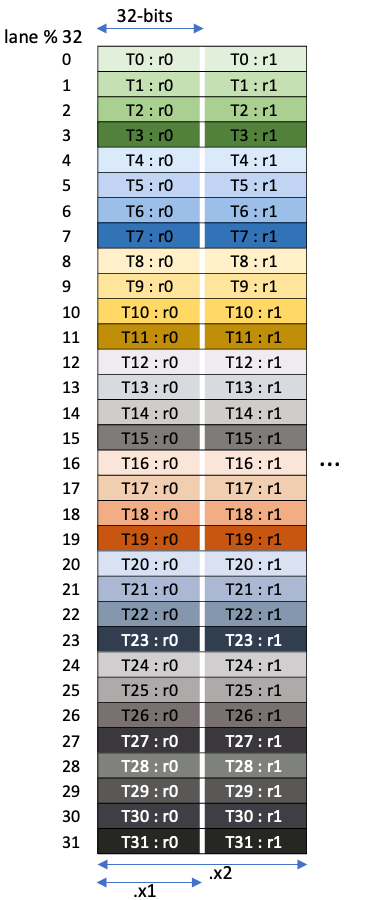
\includegraphics[width=0.3\textwidth]{figures/tikz/wp-tcgen05-tmem-fragment-3232b.png}
    \caption{\texttt{tcgen05\{.ld,.st\}.32x32b.\{x1,x2\}}}
    \label{fig:tmem_fragment-32x32}
\end{subfigure}
\hfill
\begin{subfigure}[b]{0.45\textwidth}
    \centering
    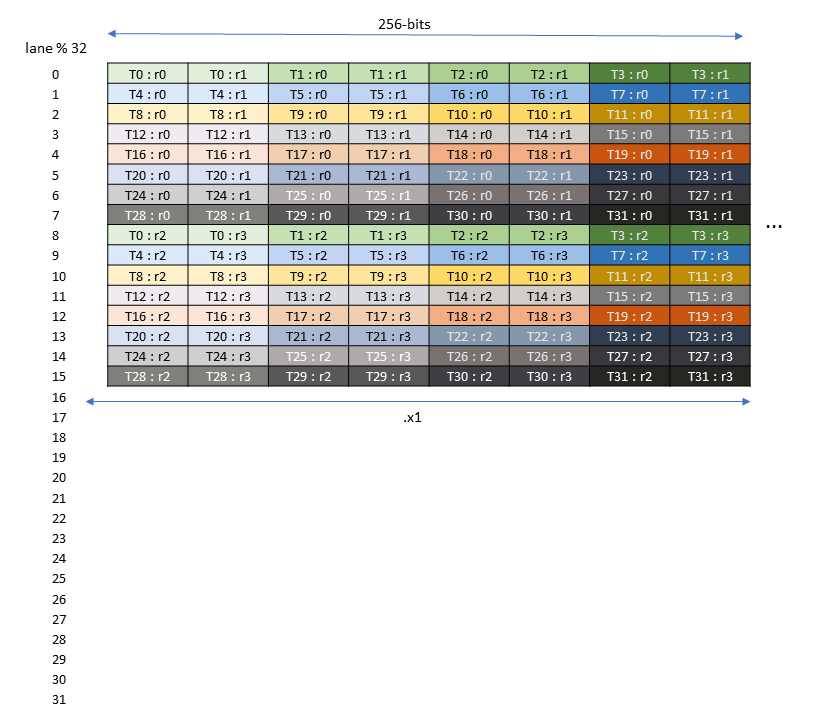
\includegraphics[width=0.8\textwidth]{figures/tikz/wp-tcgen05-tmem-fragment-16256b.png}
    \caption{\texttt{tcgen05\{.ld,.st\}.16x256b.x1}}
    \label{fig:tmem-fragment-16x256}
\end{subfigure}
\caption{TMEM load/store 指令访问特定的偏移，并将数据分配到线程本地寄存器（NVIDIA Corporation 2025）。}
\label{fig:tmem-fragments}
\end{figure}

向 Blackwell 的“张量内存”（tensor memory，TMEM）加载以及从其存储数据所使用的指令，会以一组预定义且非常特定的偏移访问 TMEM，如图~\ref{fig:tmem-fragments} 所示。物理 TMEM 的编址是一个二维网格，最多包含 512 个“列”（col）与 128 个“通道”（lane）。图中是每条指令单个 warp 的访问模式；每条指令实际使用四个 warp，上述模式每 32 个通道重复一次、共重复四次。在对物理 TMEM 编址时，沿 32 位的“列”方向跨越一步使 TMEM 地址增加 1，沿“通道”方向向下跨越一步使 TMEM 地址增加 16384。基于这一物理编址，我们定义记录每条指令所访问的全部物理偏移的布局：
\begin{center}
\begin{tabular}{l | r@{:}l}
\quad\quad\quad\quad \textbf{指令} & \multicolumn{2}{c}{$(\text{指令 COL}, \text{指令 LANE}) \to \text{TMEM 偏移}$} \\
\hline
\texttt{tcgen05\{.ld,.st\}.32x32b.x1} & $(1,128)$ & $(1,16384)$ \\
\texttt{tcgen05\{.ld,.st\}.32x32b.x2} & $(2,128)$ & $(1,16384)$ \\
\texttt{tcgen05\{.ld,.st\}.16x256b.x1} & $(8,(16,4))$ & $(1,(16384,32\cdot 16384))$ \\
\end{tabular}
\end{center}
这些布局与具体指令一一对应，可用来精确确定每条指令将访问 TMEM 中的哪些偏移。

尽管 TMEM 采用二维编址，并被用作形状为 $(M,N)$ 的 MMA 的累加器，TMEM 的“通道”与“列”并不总与逻辑矩阵的行和列相对应。与任何编址方式一样，物理偏移可以通过任意的 \CuTe{} 布局被回绕并折叠成任意形状。因此，给定一个数据布局与一条 TMEM 指令，我们希望确定
\begin{enumerate}[itemsep=0pt,topsep=2pt]
\item 数据布局是否包含该指令将访问的全部偏移；以及
\item 指令所访问的偏移在数据布局中位于何处（以逻辑坐标表示）。
\end{enumerate}

一般地，设数据布局 $\v{A} : \Z(\v{A}) \to \Z_\alpha$ 将逻辑坐标映射到数据偏移，指令布局 $\v{T} : \Z(\v{T}) \to \Z_\beta$ 将指令坐标映射到数据偏移，我们希望确定所有偏移 $\v{T}(i)$ 在 $\v{A}$ 的像中的存在性及其位置。将其表述为
\begin{align*}
\forall i \in \Z_{\abs{\v{T}}}, \exists c \in \Z(\v{A}) \ \ s.t. \ \ \v{T}(i) = \v{A}(c)
\end{align*}
该问题可以通过计算 $\v{A}$ 的左逆并检验下式来高效求解：
\begin{align*}
\v{A}(\v{A}^\dagger(\v{T}(i))) = \v{T}(i)
\end{align*}
也就是说，
\begin{compactitem}
\item 所有偏移 $\v{T}(i)$ 都在 $\v{A}^\dagger$ 的定义域中。
\item 所有坐标 $\v{A}^\dagger(\v{T}(i))$ 都互不相同，且都在 $\v{A}$ 的定义域中。
\end{compactitem}
在这些条件下，我们可以断言：每个偏移 $\v{T}(i)$ 都出现在 $\v{A}$ 的像中，且位于坐标 $\v{A}^\dagger(\v{T}(i))$ 处。布局 $\v{A}^\dagger \circ \v{T}$ 把指令坐标映射到逻辑数据坐标，例如可借助 {\tt zipped\_divide} 把数据布局 $\v{A}$ 切分为与该指令所访问偏移相对应的若干子布局。

%% wp7 补布局、逻辑乘积/逻辑切分、结论与致谢（论文收尾）
\wpsh{补}
\label{sec:complement}

布局（layout）$\v{L} : \Z(\v{L}) \to \D$ 的\emph{补}（complement）是一个满足下列条件的布局 $\v{L}^* : \Z(\v{L}^*) \to \D$
\begin{align}
\label{eqn:comp:congruence}
\text{与陪域弱同余：} && \D \lesssim \v{L}^*, \\
\label{eqn:comp:disjoint}
\text{像互不相交：} && \forall b \in \Z(\v{L}), \ \forall a \in \Z^{\v{L}^*}/\{0\}, \ &\v{L}(b) \neq \v{L}^*(a), \\
\label{eqn:comp:ordered}
\text{像有序：} && \forall a \in \Z_{\abs{\v{L}^*}}/\{0\}, \ &\v{L}^*(a-1) < \v{L}^*(a).
%\text{\emph{???:}} && \v{L}^\dagger (\v{L}, \v{L}^*) \v{L}^\dagger = \v{L}^\dagger
\end{align}
布局的补是一个在原布局的陪域（codomain）之中、但不在其像（image）之中生成元素的布局。在复合（Composition）中，布局 $\v{L}$ 常被用作对另一个布局的间接寻址，因此补 $\v{L}^*$ 就是指向 $\v{L}$ 所遗漏元素的那个布局。{\tt complement} 操作使得可以经由\emph{逻辑切分}（logical divide）（第~\ref{sec:logical_divide}~节）切分布局，并经由\emph{逻辑乘积}（logical product）（第~\ref{sec:logical_product}~节）实现布局的重复与扩展。

本节只关注陪域 $\D$ 为 {\tt HTuple}($\Z$) 的布局：即整数，或对某个轮廓 D 而言 $\D = \Z^D$ 的坐标。这使得弱同余条件式~\eqref{eqn:comp:congruence} 得以成立。像互不相交条件（式~\eqref{eqn:comp:disjoint}）保证补所生成的值与原布局生成的值互不相同。注意，这里使用的是原布局的有限定义域 $\Z(\v{L})$，而使用的是补的无穷扩展定义域 $\Z^{\v{L}^*}$。这保证了无论补的形状被截断还是被扩展（例如通过与右侧的布局复合），它所生成的值始终与原布局不同。最后，像有序条件（式~\eqref{eqn:comp:ordered}）确立了补布局的唯一性。

表~\ref{tab:complements} 给出了补的若干例子。

\begin{table}[ht]
\begin{center}
\begin{tabular}{|>{$}c<{$}|>{$}c<{$}|c|}
\v{L} & \v{L}^* & 备注 \\ \hline \hline
(4,8):(1,4) & 1:32 & 注意 $\forall i \in \Z^+, \v{L}^*(i) > \max_{j \in \Z_\v{L}} \v{L}(j)$。 \\ \hline
(4,8):(8,1) & 1:32 & 输入的顺序无关紧要。 \\ \hline
(4,(4,2)):(4,(1,16)) & 1:32 & 输入的层级结构无关紧要。 \\ \hline
(4,8):(1,5) & 1:40 \\ \hline
(4,8):(1,8) & (2,1):(4,64) & 仍然互不相交，但在陪域中“填补空洞”。 \\ \hline
((2,2),(2,4)):((0,1),(0,2)) & 1:8 & 步幅（stride）为 0 的模无贡献。 \\ \hline
((2,2),(2,4)):((0,2),(0,4)) & (2,1):(1,16) \\ \hline
(4,8):(e_0,e_1) & (1,1):(4e_0,8e_1) & 结果定义域与陪域 $\Z^{(\ast,\ast)}$ 同余。 \\ \hline
(4,(4,2)):(e_1,(e_0,12e_1)) & (1,(3,1)):(4e_0,(4e_1,24e_1)) & 弱同余、互不相交且有序。 \\ \hline
\end{tabular}
\end{center}
\caption{布局补的例子。}
\label{tab:complements}
\end{table}

\wpssh{应用：逻辑乘积}
\label{sec:logical_product}

两个布局 $\v{A}$ 与 $\v{B}$ 的逻辑乘积是一个布局 $\v{R}$，其中“布局 $\v{B}$ 的每个元素都被替换为布局 $\v{A}$ 的一个经过唯一平移的版本”。

具体地，我们将逻辑乘积定义为一个从两个布局产生一个 2 阶（rank-2）布局的函数
\begin{align*}
\v{A} \otimes \v{B} = (\v{A}, \v{A}^* \circ \v{B})
\end{align*}
其中 $\v{A}^*$ 是 $\v{A}$ 的补。注意，结果的第一个模（mode）恰好就是输入布局 $\v{A}$，而第二个模在元素形状（shape）与元素顺序上与输入布局 $\v{B}$ 相容。第一个模，即 $\v{A}$ 布局，通常被称为“瓦片”，它在“网格”布局 $\v{B}$ 上被重复。%Because the purpose of the logical product is to expand the domain and codomain of $\v{A}$, this does not require that $(\v{A},\v{A}^*)$ is surjective onto $\Z_{\norm{\v{B}}}$.

考虑这样的例子：行主序（row-major）布局 $(\textcolor{red}{3},\textcolor{red}{4}):(\textcolor{red}{4},\textcolor{red}{1})$ 瓦片，要在列主序（col-major）布局 $(\textcolor{blue}{2},\textcolor{blue}{5}):(\textcolor{blue}{1},\textcolor{blue}{2})$ 网格中复现：
\begin{align*}
\begin{array}{cc} (\textcolor{red}{3}, & \textcolor{red}{4}) \\ (\textcolor{red}{4}, & \textcolor{red}{1}) \end{array}
\ \otimes \
\begin{array}{cc} (\textcolor{blue}{2}, & \textcolor{blue}{5}) \\ (\textcolor{blue}{1}, & \textcolor{blue}{2}) \end{array}
\ =\
\left(
\begin{array}{cc} (\textcolor{red}{3}, & \textcolor{red}{4}) \\ (\textcolor{red}{4}, & \textcolor{red}{1}) \end{array}, \
\begin{array}{c} 1 \\ 12 \end{array}
\ \circ \
\begin{array}{cc}(\textcolor{blue}{2}, & \textcolor{blue}{5}) \\ (\textcolor{blue}{1},& \textcolor{blue}{2}) \end{array}
\right)
\ = \
\begin{array}{cccc}((\textcolor{red}{3}, & \textcolor{red}{4}), & (\textcolor{blue}{2}, & \textcolor{blue}{5})) \\ ((\textcolor{red}{4}, & \textcolor{red}{1}), & (\textcolor{blue}{12}, & \textcolor{blue}{24})) \end{array}
\end{align*}
其中布局 $1:12$ 是 $(\textcolor{red}{3},\textcolor{red}{4}):(\textcolor{red}{4},\textcolor{red}{1})$ 的补。在结果的第一个模中可以直接得到原始瓦片，而结果的第二个模以 $2\times 5$ 列主序的顺序将原始瓦片不重复地重复 10 次。

作为另一个例子，考虑布局 $(\textcolor{red}{4},\textcolor{red}{8}):(\textcolor{red}{20},\textcolor{red}{2})$ 瓦片在行主序布局 $(\textcolor{blue}{3},\textcolor{blue}{2}):(\textcolor{blue}{2},\textcolor{blue}{1})$ 网格中复现：
\begin{align*}
\begin{array}{cc} (\textcolor{red}{4}, & \textcolor{red}{8}) \\ (\textcolor{red}{20}, & \textcolor{red}{2}) \end{array}
\ \otimes \
\begin{array}{cc} (\textcolor{blue}{3}, & \textcolor{blue}{2}) \\ (\textcolor{blue}{2}, & \textcolor{blue}{1}) \end{array}
\ = \
\left(
\begin{array}{cc} (\textcolor{red}{4}, & \textcolor{red}{8}) \\ (\textcolor{red}{20}, & \textcolor{red}{2}) \end{array}, \
\begin{array}{cc} (2, & 1) \\ (1, & 80) \end{array}
\ \circ \
\begin{array}{cc} (\textcolor{blue}{3}, & \textcolor{blue}{2}) \\ (\textcolor{blue}{2}, & \textcolor{blue}{1}) \end{array}
\right)
\ = \
\begin{array}{cccc}((\textcolor{red}{4}, & \textcolor{red}{8}), & (\textcolor{blue}{3}, & \textcolor{blue}{2})) \\ ((\textcolor{red}{20}, & \textcolor{red}{2}), & (\textcolor{blue}{80}, & \textcolor{blue}{1})) \end{array}
\end{align*}
其中布局 $(2,1):(1,80)$ 是 $(\textcolor{red}{4},\textcolor{red}{8}):(\textcolor{red}{20},\textcolor{red}{2})$ 的补。注意，此时网格在交错排布这些瓦片，以产生结果的最小陪域。补布局告诉结果如何为布局 $\v{B}$ 设定步幅，而布局 $\v{B}$ 告诉结果如何为补布局排序并定形。

\paragraph{相关乘积}

逻辑乘积产生一个 2 阶布局，其中第一个模是原始瓦片，第二个模被解释为该瓦片的网格，即“铺瓦”。

虽然逻辑乘积对 $\v{A}$ 与 $\v{B}$ 的阶（rank）或相容性没有任何限制，但操作 {\tt blocked\_product} 往往是一个更直观的版本，它利用输入的阶来构造结果的形状。我们可能会期望一个 $3 {\times} 4$ 布局与一个 $2 {\times} 5$ 布局的乘积产生一个 $6 {\times} 20$ 布局。{\tt blocked\_product} 要求 $\v{A}$ 与 $\v{B}$ 的阶相同，
\begin{align*}
\text{阶}(\v{A}) = \text{阶}(\v{B})
\end{align*}
以便施加一个 zip 操作，把逻辑上的行模与行模、列模与列模组合起来。例如，将上例中的模重排
\begin{align*}
\begin{array}{cccc}((\textcolor{red}{3}, & \textcolor{red}{4}), & (\textcolor{blue}{2}, & \textcolor{blue}{5})) \\ ((\textcolor{red}{4}, & \textcolor{red}{1}), & (\textcolor{blue}{12}, & \textcolor{blue}{24})) \end{array}
\ \Longrightarrow \
\begin{array}{cccc}((\textcolor{red}{3}, & \textcolor{blue}{2}), & (\textcolor{red}{4}, & \textcolor{blue}{5})) \\ ((\textcolor{red}{4}, & \textcolor{blue}{12}), & (\textcolor{red}{1}, & \textcolor{blue}{24})) \end{array}
\end{align*}
便得到一个 $6 {\times} 20$ 布局。图~\ref{fig:blockedproduct} 画出了得到的布局，其中每个 $3 {\times} 4$ 瓦片都施以底纹。之所以称其为“分块”，是因为结果布局中的每个 $3 {\times} 4$ 块都恰好是原始 $3 {\times} 4$ 瓦片的平移版本。

\begin{figure}[ht]
\centering
%\includegraphics[scale=0.5]{blocked_product}
\scalebox{0.5}{
\begin{tikzpicture}[x={(0cm,-1cm)},y={(1cm,0cm)},every node/.style={minimum size=1cm, outer sep=0pt}]
\node[fill={rgb,255:red,255;green,255;blue,255}] at (0,0) {\large 0};
\node[fill={rgb,255:red,255;green,255;blue,255}] at (0,1) {\large 1};
\node[fill={rgb,255:red,255;green,255;blue,255}] at (0,2) {\large 2};
\node[fill={rgb,255:red,255;green,255;blue,255}] at (0,3) {\large 3};
\node[fill={rgb,255:red,210;green,210;blue,255}] at (0,4) {\large 24};
\node[fill={rgb,255:red,210;green,210;blue,255}] at (0,5) {\large 25};
\node[fill={rgb,255:red,210;green,210;blue,255}] at (0,6) {\large 26};
\node[fill={rgb,255:red,210;green,210;blue,255}] at (0,7) {\large 27};
\node[fill={rgb,255:red,210;green,255;blue,210}] at (0,8) {\large 48};
\node[fill={rgb,255:red,210;green,255;blue,210}] at (0,9) {\large 49};
\node[fill={rgb,255:red,210;green,255;blue,210}] at (0,10) {\large 50};
\node[fill={rgb,255:red,210;green,255;blue,210}] at (0,11) {\large 51};
\node[fill={rgb,255:red,255;green,255;blue,210}] at (0,12) {\large 72};
\node[fill={rgb,255:red,255;green,255;blue,210}] at (0,13) {\large 73};
\node[fill={rgb,255:red,255;green,255;blue,210}] at (0,14) {\large 74};
\node[fill={rgb,255:red,255;green,255;blue,210}] at (0,15) {\large 75};
\node[fill={rgb,255:red,255;green,210;blue,210}] at (0,16) {\large 96};
\node[fill={rgb,255:red,255;green,210;blue,210}] at (0,17) {\large 97};
\node[fill={rgb,255:red,255;green,210;blue,210}] at (0,18) {\large 98};
\node[fill={rgb,255:red,255;green,210;blue,210}] at (0,19) {\large 99};
\node[fill={rgb,255:red,255;green,255;blue,255}] at (1,0) {\large 4};
\node[fill={rgb,255:red,255;green,255;blue,255}] at (1,1) {\large 5};
\node[fill={rgb,255:red,255;green,255;blue,255}] at (1,2) {\large 6};
\node[fill={rgb,255:red,255;green,255;blue,255}] at (1,3) {\large 7};
\node[fill={rgb,255:red,210;green,210;blue,255}] at (1,4) {\large 28};
\node[fill={rgb,255:red,210;green,210;blue,255}] at (1,5) {\large 29};
\node[fill={rgb,255:red,210;green,210;blue,255}] at (1,6) {\large 30};
\node[fill={rgb,255:red,210;green,210;blue,255}] at (1,7) {\large 31};
\node[fill={rgb,255:red,210;green,255;blue,210}] at (1,8) {\large 52};
\node[fill={rgb,255:red,210;green,255;blue,210}] at (1,9) {\large 53};
\node[fill={rgb,255:red,210;green,255;blue,210}] at (1,10) {\large 54};
\node[fill={rgb,255:red,210;green,255;blue,210}] at (1,11) {\large 55};
\node[fill={rgb,255:red,255;green,255;blue,210}] at (1,12) {\large 76};
\node[fill={rgb,255:red,255;green,255;blue,210}] at (1,13) {\large 77};
\node[fill={rgb,255:red,255;green,255;blue,210}] at (1,14) {\large 78};
\node[fill={rgb,255:red,255;green,255;blue,210}] at (1,15) {\large 79};
\node[fill={rgb,255:red,255;green,210;blue,210}] at (1,16) {\large 100};
\node[fill={rgb,255:red,255;green,210;blue,210}] at (1,17) {\large 101};
\node[fill={rgb,255:red,255;green,210;blue,210}] at (1,18) {\large 102};
\node[fill={rgb,255:red,255;green,210;blue,210}] at (1,19) {\large 103};
\node[fill={rgb,255:red,255;green,255;blue,255}] at (2,0) {\large 8};
\node[fill={rgb,255:red,255;green,255;blue,255}] at (2,1) {\large 9};
\node[fill={rgb,255:red,255;green,255;blue,255}] at (2,2) {\large 10};
\node[fill={rgb,255:red,255;green,255;blue,255}] at (2,3) {\large 11};
\node[fill={rgb,255:red,210;green,210;blue,255}] at (2,4) {\large 32};
\node[fill={rgb,255:red,210;green,210;blue,255}] at (2,5) {\large 33};
\node[fill={rgb,255:red,210;green,210;blue,255}] at (2,6) {\large 34};
\node[fill={rgb,255:red,210;green,210;blue,255}] at (2,7) {\large 35};
\node[fill={rgb,255:red,210;green,255;blue,210}] at (2,8) {\large 56};
\node[fill={rgb,255:red,210;green,255;blue,210}] at (2,9) {\large 57};
\node[fill={rgb,255:red,210;green,255;blue,210}] at (2,10) {\large 58};
\node[fill={rgb,255:red,210;green,255;blue,210}] at (2,11) {\large 59};
\node[fill={rgb,255:red,255;green,255;blue,210}] at (2,12) {\large 80};
\node[fill={rgb,255:red,255;green,255;blue,210}] at (2,13) {\large 81};
\node[fill={rgb,255:red,255;green,255;blue,210}] at (2,14) {\large 82};
\node[fill={rgb,255:red,255;green,255;blue,210}] at (2,15) {\large 83};
\node[fill={rgb,255:red,255;green,210;blue,210}] at (2,16) {\large 104};
\node[fill={rgb,255:red,255;green,210;blue,210}] at (2,17) {\large 105};
\node[fill={rgb,255:red,255;green,210;blue,210}] at (2,18) {\large 106};
\node[fill={rgb,255:red,255;green,210;blue,210}] at (2,19) {\large 107};
\node[fill={rgb,255:red,175;green,175;blue,175}] at (3,0) {\large 12};
\node[fill={rgb,255:red,175;green,175;blue,175}] at (3,1) {\large 13};
\node[fill={rgb,255:red,175;green,175;blue,175}] at (3,2) {\large 14};
\node[fill={rgb,255:red,175;green,175;blue,175}] at (3,3) {\large 15};
\node[fill={rgb,255:red,175;green,175;blue,255}] at (3,4) {\large 36};
\node[fill={rgb,255:red,175;green,175;blue,255}] at (3,5) {\large 37};
\node[fill={rgb,255:red,175;green,175;blue,255}] at (3,6) {\large 38};
\node[fill={rgb,255:red,175;green,175;blue,255}] at (3,7) {\large 39};
\node[fill={rgb,255:red,175;green,255;blue,175}] at (3,8) {\large 60};
\node[fill={rgb,255:red,175;green,255;blue,175}] at (3,9) {\large 61};
\node[fill={rgb,255:red,175;green,255;blue,175}] at (3,10) {\large 62};
\node[fill={rgb,255:red,175;green,255;blue,175}] at (3,11) {\large 63};
\node[fill={rgb,255:red,255;green,255;blue,175}] at (3,12) {\large 84};
\node[fill={rgb,255:red,255;green,255;blue,175}] at (3,13) {\large 85};
\node[fill={rgb,255:red,255;green,255;blue,175}] at (3,14) {\large 86};
\node[fill={rgb,255:red,255;green,255;blue,175}] at (3,15) {\large 87};
\node[fill={rgb,255:red,255;green,175;blue,175}] at (3,16) {\large 108};
\node[fill={rgb,255:red,255;green,175;blue,175}] at (3,17) {\large 109};
\node[fill={rgb,255:red,255;green,175;blue,175}] at (3,18) {\large 110};
\node[fill={rgb,255:red,255;green,175;blue,175}] at (3,19) {\large 111};
\node[fill={rgb,255:red,175;green,175;blue,175}] at (4,0) {\large 16};
\node[fill={rgb,255:red,175;green,175;blue,175}] at (4,1) {\large 17};
\node[fill={rgb,255:red,175;green,175;blue,175}] at (4,2) {\large 18};
\node[fill={rgb,255:red,175;green,175;blue,175}] at (4,3) {\large 19};
\node[fill={rgb,255:red,175;green,175;blue,255}] at (4,4) {\large 40};
\node[fill={rgb,255:red,175;green,175;blue,255}] at (4,5) {\large 41};
\node[fill={rgb,255:red,175;green,175;blue,255}] at (4,6) {\large 42};
\node[fill={rgb,255:red,175;green,175;blue,255}] at (4,7) {\large 43};
\node[fill={rgb,255:red,175;green,255;blue,175}] at (4,8) {\large 64};
\node[fill={rgb,255:red,175;green,255;blue,175}] at (4,9) {\large 65};
\node[fill={rgb,255:red,175;green,255;blue,175}] at (4,10) {\large 66};
\node[fill={rgb,255:red,175;green,255;blue,175}] at (4,11) {\large 67};
\node[fill={rgb,255:red,255;green,255;blue,175}] at (4,12) {\large 88};
\node[fill={rgb,255:red,255;green,255;blue,175}] at (4,13) {\large 89};
\node[fill={rgb,255:red,255;green,255;blue,175}] at (4,14) {\large 90};
\node[fill={rgb,255:red,255;green,255;blue,175}] at (4,15) {\large 91};
\node[fill={rgb,255:red,255;green,175;blue,175}] at (4,16) {\large 112};
\node[fill={rgb,255:red,255;green,175;blue,175}] at (4,17) {\large 113};
\node[fill={rgb,255:red,255;green,175;blue,175}] at (4,18) {\large 114};
\node[fill={rgb,255:red,255;green,175;blue,175}] at (4,19) {\large 115};
\node[fill={rgb,255:red,175;green,175;blue,175}] at (5,0) {\large 20};
\node[fill={rgb,255:red,175;green,175;blue,175}] at (5,1) {\large 21};
\node[fill={rgb,255:red,175;green,175;blue,175}] at (5,2) {\large 22};
\node[fill={rgb,255:red,175;green,175;blue,175}] at (5,3) {\large 23};
\node[fill={rgb,255:red,175;green,175;blue,255}] at (5,4) {\large 44};
\node[fill={rgb,255:red,175;green,175;blue,255}] at (5,5) {\large 45};
\node[fill={rgb,255:red,175;green,175;blue,255}] at (5,6) {\large 46};
\node[fill={rgb,255:red,175;green,175;blue,255}] at (5,7) {\large 47};
\node[fill={rgb,255:red,175;green,255;blue,175}] at (5,8) {\large 68};
\node[fill={rgb,255:red,175;green,255;blue,175}] at (5,9) {\large 69};
\node[fill={rgb,255:red,175;green,255;blue,175}] at (5,10) {\large 70};
\node[fill={rgb,255:red,175;green,255;blue,175}] at (5,11) {\large 71};
\node[fill={rgb,255:red,255;green,255;blue,175}] at (5,12) {\large 92};
\node[fill={rgb,255:red,255;green,255;blue,175}] at (5,13) {\large 93};
\node[fill={rgb,255:red,255;green,255;blue,175}] at (5,14) {\large 94};
\node[fill={rgb,255:red,255;green,255;blue,175}] at (5,15) {\large 95};
\node[fill={rgb,255:red,255;green,175;blue,175}] at (5,16) {\large 116};
\node[fill={rgb,255:red,255;green,175;blue,175}] at (5,17) {\large 117};
\node[fill={rgb,255:red,255;green,175;blue,175}] at (5,18) {\large 118};
\node[fill={rgb,255:red,255;green,175;blue,175}] at (5,19) {\large 119};
\draw[color=black,thick,shift={(-0.5,-0.5)}] (0,0) grid (6,20);

\node at (0,-1) {\Large{\texttt{0}}};
\node at (1,-1) {\Large{\texttt{1}}};
\node at (2,-1) {\Large{\texttt{2}}};
\node at (3,-1) {\Large{\texttt{3}}};
\node at (4,-1) {\Large{\texttt{4}}};
\node at (5,-1) {\Large{\texttt{5}}};
\node at (-1,0) {\Large{\texttt{0}}};
\node at (-1,1) {\Large{\texttt{1}}};
\node at (-1,2) {\Large{\texttt{2}}};
\node at (-1,3) {\Large{\texttt{3}}};
\node at (-1,4) {\Large{\texttt{4}}};
\node at (-1,5) {\Large{\texttt{5}}};
\node at (-1,6) {\Large{\texttt{6}}};
\node at (-1,7) {\Large{\texttt{7}}};
\node at (-1,8) {\Large{\texttt{8}}};
\node at (-1,9) {\Large{\texttt{9}}};
\node at (-1,10) {\Large{\texttt{10}}};
\node at (-1,11) {\Large{\texttt{11}}};
\node at (-1,12) {\Large{\texttt{12}}};
\node at (-1,13) {\Large{\texttt{13}}};
\node at (-1,14) {\Large{\texttt{14}}};
\node at (-1,15) {\Large{\texttt{15}}};
\node at (-1,16) {\Large{\texttt{16}}};
\node at (-1,17) {\Large{\texttt{17}}};
\node at (-1,18) {\Large{\texttt{18}}};
\node at (-1,19) {\Large{\texttt{19}}};
\end{tikzpicture}
}
\caption{行主序 $(3,4):(4,1)$ 瓦片与列主序 $(2,5):(1,2)$ 铺瓦的 {\tt blocked\_product}。}
\label{fig:blockedproduct}
\end{figure}

操作 {\tt raked\_product} 与分块乘积类似，只是各模以相反的顺序拉链（zip）组合：
\begin{align*}
\begin{array}{cccc}((\textcolor{red}{3}, & \textcolor{red}{4}), & (\textcolor{blue}{2}, & \textcolor{blue}{5})) \\ ((\textcolor{red}{4}, & \textcolor{red}{1}), & (\textcolor{blue}{12}, & \textcolor{blue}{24})) \end{array}
\ \Longrightarrow \
\begin{array}{cccc}((\textcolor{blue}{2}, & \textcolor{red}{3}), & (\textcolor{blue}{5}, & \textcolor{red}{4})) \\ ((\textcolor{blue}{12}, & \textcolor{red}{4}), & (\textcolor{blue}{24}, & \textcolor{red}{1})) \end{array}
\end{align*}
其效果是 $3 {\times} 4$ 瓦片被“耙”（raked）在 $2 {\times} 5$ 瓦片之上，而非“分块”排布。图~\ref{fig:rakedproduct} 画出了得到的布局，其中每个 $3 {\times} 4$ 瓦片都施以底纹。

\begin{figure}[ht]
\centering
%\includegraphics[scale=0.5]{raked_product}
\scalebox{0.5}{
\begin{tikzpicture}[x={(0cm,-1cm)},y={(1cm,0cm)},every node/.style={minimum size=1cm, outer sep=0pt}]

\node[fill={rgb,255:red,255;green,255;blue,255}] at (0,0) {\large 0};
\node[fill={rgb,255:red,210;green,210;blue,255}] at (0,1) {\large 24};
\node[fill={rgb,255:red,210;green,255;blue,210}] at (0,2) {\large 48};
\node[fill={rgb,255:red,255;green,255;blue,210}] at (0,3) {\large 72};
\node[fill={rgb,255:red,255;green,210;blue,210}] at (0,4) {\large 96};
\node[fill={rgb,255:red,255;green,255;blue,255}] at (0,5) {\large 1};
\node[fill={rgb,255:red,210;green,210;blue,255}] at (0,6) {\large 25};
\node[fill={rgb,255:red,210;green,255;blue,210}] at (0,7) {\large 49};
\node[fill={rgb,255:red,255;green,255;blue,210}] at (0,8) {\large 73};
\node[fill={rgb,255:red,255;green,210;blue,210}] at (0,9) {\large 97};
\node[fill={rgb,255:red,255;green,255;blue,255}] at (0,10) {\large 2};
\node[fill={rgb,255:red,210;green,210;blue,255}] at (0,11) {\large 26};
\node[fill={rgb,255:red,210;green,255;blue,210}] at (0,12) {\large 50};
\node[fill={rgb,255:red,255;green,255;blue,210}] at (0,13) {\large 74};
\node[fill={rgb,255:red,255;green,210;blue,210}] at (0,14) {\large 98};
\node[fill={rgb,255:red,255;green,255;blue,255}] at (0,15) {\large 3};
\node[fill={rgb,255:red,210;green,210;blue,255}] at (0,16) {\large 27};
\node[fill={rgb,255:red,210;green,255;blue,210}] at (0,17) {\large 51};
\node[fill={rgb,255:red,255;green,255;blue,210}] at (0,18) {\large 75};
\node[fill={rgb,255:red,255;green,210;blue,210}] at (0,19) {\large 99};
\node[fill={rgb,255:red,175;green,175;blue,175}] at (1,0) {\large 12};
\node[fill={rgb,255:red,175;green,175;blue,255}] at (1,1) {\large 36};
\node[fill={rgb,255:red,175;green,255;blue,175}] at (1,2) {\large 60};
\node[fill={rgb,255:red,255;green,255;blue,175}] at (1,3) {\large 84};
\node[fill={rgb,255:red,255;green,175;blue,175}] at (1,4) {\large 108};
\node[fill={rgb,255:red,175;green,175;blue,175}] at (1,5) {\large 13};
\node[fill={rgb,255:red,175;green,175;blue,255}] at (1,6) {\large 37};
\node[fill={rgb,255:red,175;green,255;blue,175}] at (1,7) {\large 61};
\node[fill={rgb,255:red,255;green,255;blue,175}] at (1,8) {\large 85};
\node[fill={rgb,255:red,255;green,175;blue,175}] at (1,9) {\large 109};
\node[fill={rgb,255:red,175;green,175;blue,175}] at (1,10) {\large 14};
\node[fill={rgb,255:red,175;green,175;blue,255}] at (1,11) {\large 38};
\node[fill={rgb,255:red,175;green,255;blue,175}] at (1,12) {\large 62};
\node[fill={rgb,255:red,255;green,255;blue,175}] at (1,13) {\large 86};
\node[fill={rgb,255:red,255;green,175;blue,175}] at (1,14) {\large 110};
\node[fill={rgb,255:red,175;green,175;blue,175}] at (1,15) {\large 15};
\node[fill={rgb,255:red,175;green,175;blue,255}] at (1,16) {\large 39};
\node[fill={rgb,255:red,175;green,255;blue,175}] at (1,17) {\large 63};
\node[fill={rgb,255:red,255;green,255;blue,175}] at (1,18) {\large 87};
\node[fill={rgb,255:red,255;green,175;blue,175}] at (1,19) {\large 111};
\node[fill={rgb,255:red,255;green,255;blue,255}] at (2,0) {\large 4};
\node[fill={rgb,255:red,210;green,210;blue,255}] at (2,1) {\large 28};
\node[fill={rgb,255:red,210;green,255;blue,210}] at (2,2) {\large 52};
\node[fill={rgb,255:red,255;green,255;blue,210}] at (2,3) {\large 76};
\node[fill={rgb,255:red,255;green,210;blue,210}] at (2,4) {\large 100};
\node[fill={rgb,255:red,255;green,255;blue,255}] at (2,5) {\large 5};
\node[fill={rgb,255:red,210;green,210;blue,255}] at (2,6) {\large 29};
\node[fill={rgb,255:red,210;green,255;blue,210}] at (2,7) {\large 53};
\node[fill={rgb,255:red,255;green,255;blue,210}] at (2,8) {\large 77};
\node[fill={rgb,255:red,255;green,210;blue,210}] at (2,9) {\large 101};
\node[fill={rgb,255:red,255;green,255;blue,255}] at (2,10) {\large 6};
\node[fill={rgb,255:red,210;green,210;blue,255}] at (2,11) {\large 30};
\node[fill={rgb,255:red,210;green,255;blue,210}] at (2,12) {\large 54};
\node[fill={rgb,255:red,255;green,255;blue,210}] at (2,13) {\large 78};
\node[fill={rgb,255:red,255;green,210;blue,210}] at (2,14) {\large 102};
\node[fill={rgb,255:red,255;green,255;blue,255}] at (2,15) {\large 7};
\node[fill={rgb,255:red,210;green,210;blue,255}] at (2,16) {\large 31};
\node[fill={rgb,255:red,210;green,255;blue,210}] at (2,17) {\large 55};
\node[fill={rgb,255:red,255;green,255;blue,210}] at (2,18) {\large 79};
\node[fill={rgb,255:red,255;green,210;blue,210}] at (2,19) {\large 103};
\node[fill={rgb,255:red,175;green,175;blue,175}] at (3,0) {\large 16};
\node[fill={rgb,255:red,175;green,175;blue,255}] at (3,1) {\large 40};
\node[fill={rgb,255:red,175;green,255;blue,175}] at (3,2) {\large 64};
\node[fill={rgb,255:red,255;green,255;blue,175}] at (3,3) {\large 88};
\node[fill={rgb,255:red,255;green,175;blue,175}] at (3,4) {\large 112};
\node[fill={rgb,255:red,175;green,175;blue,175}] at (3,5) {\large 17};
\node[fill={rgb,255:red,175;green,175;blue,255}] at (3,6) {\large 41};
\node[fill={rgb,255:red,175;green,255;blue,175}] at (3,7) {\large 65};
\node[fill={rgb,255:red,255;green,255;blue,175}] at (3,8) {\large 89};
\node[fill={rgb,255:red,255;green,175;blue,175}] at (3,9) {\large 113};
\node[fill={rgb,255:red,175;green,175;blue,175}] at (3,10) {\large 18};
\node[fill={rgb,255:red,175;green,175;blue,255}] at (3,11) {\large 42};
\node[fill={rgb,255:red,175;green,255;blue,175}] at (3,12) {\large 66};
\node[fill={rgb,255:red,255;green,255;blue,175}] at (3,13) {\large 90};
\node[fill={rgb,255:red,255;green,175;blue,175}] at (3,14) {\large 114};
\node[fill={rgb,255:red,175;green,175;blue,175}] at (3,15) {\large 19};
\node[fill={rgb,255:red,175;green,175;blue,255}] at (3,16) {\large 43};
\node[fill={rgb,255:red,175;green,255;blue,175}] at (3,17) {\large 67};
\node[fill={rgb,255:red,255;green,255;blue,175}] at (3,18) {\large 91};
\node[fill={rgb,255:red,255;green,175;blue,175}] at (3,19) {\large 115};
\node[fill={rgb,255:red,255;green,255;blue,255}] at (4,0) {\large 8};
\node[fill={rgb,255:red,210;green,210;blue,255}] at (4,1) {\large 32};
\node[fill={rgb,255:red,210;green,255;blue,210}] at (4,2) {\large 56};
\node[fill={rgb,255:red,255;green,255;blue,210}] at (4,3) {\large 80};
\node[fill={rgb,255:red,255;green,210;blue,210}] at (4,4) {\large 104};
\node[fill={rgb,255:red,255;green,255;blue,255}] at (4,5) {\large 9};
\node[fill={rgb,255:red,210;green,210;blue,255}] at (4,6) {\large 33};
\node[fill={rgb,255:red,210;green,255;blue,210}] at (4,7) {\large 57};
\node[fill={rgb,255:red,255;green,255;blue,210}] at (4,8) {\large 81};
\node[fill={rgb,255:red,255;green,210;blue,210}] at (4,9) {\large 105};
\node[fill={rgb,255:red,255;green,255;blue,255}] at (4,10) {\large 10};
\node[fill={rgb,255:red,210;green,210;blue,255}] at (4,11) {\large 34};
\node[fill={rgb,255:red,210;green,255;blue,210}] at (4,12) {\large 58};
\node[fill={rgb,255:red,255;green,255;blue,210}] at (4,13) {\large 82};
\node[fill={rgb,255:red,255;green,210;blue,210}] at (4,14) {\large 106};
\node[fill={rgb,255:red,255;green,255;blue,255}] at (4,15) {\large 11};
\node[fill={rgb,255:red,210;green,210;blue,255}] at (4,16) {\large 35};
\node[fill={rgb,255:red,210;green,255;blue,210}] at (4,17) {\large 59};
\node[fill={rgb,255:red,255;green,255;blue,210}] at (4,18) {\large 83};
\node[fill={rgb,255:red,255;green,210;blue,210}] at (4,19) {\large 107};
\node[fill={rgb,255:red,175;green,175;blue,175}] at (5,0) {\large 20};
\node[fill={rgb,255:red,175;green,175;blue,255}] at (5,1) {\large 44};
\node[fill={rgb,255:red,175;green,255;blue,175}] at (5,2) {\large 68};
\node[fill={rgb,255:red,255;green,255;blue,175}] at (5,3) {\large 92};
\node[fill={rgb,255:red,255;green,175;blue,175}] at (5,4) {\large 116};
\node[fill={rgb,255:red,175;green,175;blue,175}] at (5,5) {\large 21};
\node[fill={rgb,255:red,175;green,175;blue,255}] at (5,6) {\large 45};
\node[fill={rgb,255:red,175;green,255;blue,175}] at (5,7) {\large 69};
\node[fill={rgb,255:red,255;green,255;blue,175}] at (5,8) {\large 93};
\node[fill={rgb,255:red,255;green,175;blue,175}] at (5,9) {\large 117};
\node[fill={rgb,255:red,175;green,175;blue,175}] at (5,10) {\large 22};
\node[fill={rgb,255:red,175;green,175;blue,255}] at (5,11) {\large 46};
\node[fill={rgb,255:red,175;green,255;blue,175}] at (5,12) {\large 70};
\node[fill={rgb,255:red,255;green,255;blue,175}] at (5,13) {\large 94};
\node[fill={rgb,255:red,255;green,175;blue,175}] at (5,14) {\large 118};
\node[fill={rgb,255:red,175;green,175;blue,175}] at (5,15) {\large 23};
\node[fill={rgb,255:red,175;green,175;blue,255}] at (5,16) {\large 47};
\node[fill={rgb,255:red,175;green,255;blue,175}] at (5,17) {\large 71};
\node[fill={rgb,255:red,255;green,255;blue,175}] at (5,18) {\large 95};
\node[fill={rgb,255:red,255;green,175;blue,175}] at (5,19) {\large 119};
\draw[color=black,thick,shift={(-0.5,-0.5)}] (0,0) grid (6,20);

\node at (0,-1) {\Large{\texttt{0}}};
\node at (1,-1) {\Large{\texttt{1}}};
\node at (2,-1) {\Large{\texttt{2}}};
\node at (3,-1) {\Large{\texttt{3}}};
\node at (4,-1) {\Large{\texttt{4}}};
\node at (5,-1) {\Large{\texttt{5}}};
\node at (-1,0) {\Large{\texttt{0}}};
\node at (-1,1) {\Large{\texttt{1}}};
\node at (-1,2) {\Large{\texttt{2}}};
\node at (-1,3) {\Large{\texttt{3}}};
\node at (-1,4) {\Large{\texttt{4}}};
\node at (-1,5) {\Large{\texttt{5}}};
\node at (-1,6) {\Large{\texttt{6}}};
\node at (-1,7) {\Large{\texttt{7}}};
\node at (-1,8) {\Large{\texttt{8}}};
\node at (-1,9) {\Large{\texttt{9}}};
\node at (-1,10) {\Large{\texttt{10}}};
\node at (-1,11) {\Large{\texttt{11}}};
\node at (-1,12) {\Large{\texttt{12}}};
\node at (-1,13) {\Large{\texttt{13}}};
\node at (-1,14) {\Large{\texttt{14}}};
\node at (-1,15) {\Large{\texttt{15}}};
\node at (-1,16) {\Large{\texttt{16}}};
\node at (-1,17) {\Large{\texttt{17}}};
\node at (-1,18) {\Large{\texttt{18}}};
\node at (-1,19) {\Large{\texttt{19}}};
\end{tikzpicture}
}
\caption{行主序 $(3,4):(4,1)$ 瓦片与列主序 $(2,5):(1,2)$ 铺瓦的 {\tt raked\_product}。}
\label{fig:rakedproduct}
\end{figure}

%The operation {\tt tiled\_product} is another convenience function that simply flattens by one level the second mode of a logical product.

还可以构造逻辑乘积的许多其它版本，它们额外地对模进行分组与重排，以得到方便使用的结果。

\wpssh{应用：逻辑切分}
\label{sec:logical_divide}

两个布局 $\v{A}$ 与 $\v{B}$ 的逻辑切分是一个布局 $\v{R}$，其中“布局 $\v{A}$ 被一分为二：被 $\v{B}$ 指向的元素与未被 $\v{B}$ 指向的元素”。

具体地，我们将逻辑切分定义为一个从两个布局产生一个 2 阶布局的函数
\begin{align*}
\v{A} \oslash \v{B} = \v{A} \circ (\v{B}, \v{B}^*_{\abs{\v{A}}}) = \v{A} \circ \v{B}^\bigstar
\end{align*}
其中 $\v{B}^*_{\abs{\v{A}}}$ 是 $\v{B}$ 相对于布局 $\v{A}$ 的尺寸所取的补。由于该操作意在保留 $\v{A}$ 的全部元素、只是把布局 $\v{A}$ 一分为二，我们要求 $\v{B}^\bigstar = (\v{B},\v{B}^*_{\abs{\v{A}}})$ 满射到 $\Z_{\abs{A}}$。这通常涉及对 $\v{B}^*$ 尺寸的扩展，使得 $\abs{\v{B}^\bigstar} \geq \abs{\v{A}}$。此外，我们要求补 $\v{B}^*$ 在如下意义上“补全”布局 $\v{B}$：$\v{B}^\bigstar = (\v{B},\v{B}^*_{\abs{A}})$ 具有自反广义逆 $\v{B}^+$，满足
\begin{align}
\v{B}^\bigstar \v{B}^+ \v{B}^\bigstar = \v{B}^\bigstar \\
\v{B}^+ \v{B}^\bigstar \v{B}^+ = \v{B}^+
\end{align}

与逻辑乘积操作类似，结果布局 $\v{A} \circ \v{B}$ 的第一个模通常被称为“瓦片”，它在“网格”（即“铺瓦”）布局 $\v{A} \circ \v{B}^*_{\abs{\v{A}}}$ 上被重复。参数 $\v{B}$ 被称为“铺瓦器”，它可以被扩展为不仅仅是布局，如第~\ref{sec:tiler}~节所述。

作为一个直接的例子，常见的需求是从另一个布局中取出某组逻辑元素。例如，要从布局中每隔三个取一个元素，可以使用复合：
\begin{align*}
\begin{array}{c} \textcolor{red}{24} \\ \textcolor{red}{3} \end{array}
\ \circ \
\begin{array}{c} \textcolor{blue}{8} \\ \textcolor{blue}{3} \end{array}
\ &= \
\begin{array}{c} \textcolor{blue}{8} \\ \textcolor{blue}{9} \end{array} \\
\begin{array}{ccc} (\textcolor{red}{6}, & \textcolor{red}{2}, & \textcolor{red}{2}) \\ (\textcolor{red}{2}, & \textcolor{red}{1}, & \textcolor{red}{20}) \end{array}
\ \circ \
\begin{array}{c} \textcolor{blue}{8} \\ \textcolor{blue}{3} \end{array}
\ &= \
\begin{array}{ccc} (\textcolor{blue}{2}, & \textcolor{blue}{2}, & \textcolor{blue}{2}) \\ (\textcolor{blue}{6}, & \textcolor{blue}{1}, & \textcolor{blue}{20}) \end{array}
\end{align*}
在上面两种情形中，都是 24 个元素的布局与布局 $8:3$ 复合，得到每隔三个取一个元素的布局。但左手边布局中“其余”的元素怎么办？逻辑切分把左手边的布局拆成两块：被右手边“命中”的部分与“其余”部分：
\begin{align*}
\begin{array}{c} \textcolor{red}{24} \\ \textcolor{red}{3} \end{array}
\ \oslash \
\begin{array}{c} \textcolor{blue}{8} \\ \textcolor{blue}{3} \end{array}
\ &=& \
\begin{array}{c} \textcolor{red}{24} \\ \textcolor{red}{3} \end{array}
\ \circ \
\begin{array}{cc} (\textcolor{blue}{8}, & 3) \\ (\textcolor{blue}{3}, & 1) \end{array}
\ &=& \
\begin{array}{cc} (\textcolor{blue}{8}, & 3) \\ (\textcolor{blue}{9}, & 3) \end{array} \\
\begin{array}{ccc} (\textcolor{red}{6}, & \textcolor{red}{2}, & \textcolor{red}{2}) \\ (\textcolor{red}{2}, & \textcolor{red}{1}, & \textcolor{red}{20}) \end{array}
\ \oslash \
\begin{array}{c} \textcolor{blue}{8} \\ \textcolor{blue}{3} \end{array}
\ &=& \
\begin{array}{ccc} (\textcolor{red}{6}, & \textcolor{red}{2}, & \textcolor{red}{2}) \\ (\textcolor{red}{2}, & \textcolor{red}{1}, & \textcolor{red}{20}) \end{array}
\ \circ \
\begin{array}{cc} (\textcolor{blue}{8}, & 3) \\ (\textcolor{blue}{3}, & 1) \end{array}
\ &=& \
\begin{array}{cccc} ((\textcolor{blue}{2}, & \textcolor{blue}{2}, & \textcolor{blue}{2}), & 3) \\ ((\textcolor{blue}{6}, & \textcolor{blue}{1}, & \textcolor{blue}{20}), & 2) \end{array}
\end{align*}
其中 $3:1$ 是 $8:3$ 在尺寸 24 之下的补。结果的第一模按要求仍然包含左手边布局中每隔三个取一个的元素，而结果的第二模是这些“瓦片”在原布局中的个数（本例中为 3）以及这些瓦片之间的步幅。补被用来确定缺失了哪些元素、以及以何种顺序保留它们。

\paragraph{相关切分}

与复合类似，人们经常希望按模施加逻辑切分。这里使用同样的记号与策略
\begin{align*}
\v{A} \oslash \langle \v{B},\v{C} \rangle = (\v{A}_0,\v{A}_1) \oslash \langle \v{B},\v{C} \rangle = (\v{A}_0 \oslash \v{B}, \v{A}_1 \oslash \v{C}).
\end{align*}
其直觉在于：能够对列和行独立地执行这些操作，然后视需要重排这些模以构造新布局，这与布局乘积类似。例如，回到第~\ref{sec:tiler}~节中的铺瓦器，将这些铺瓦器用于逻辑切分而非复合，就得到铺瓦器所指向的 $4 {\times} 8$ 子布局组成的 $2 {\times} 2$ 布局。图~\ref{fig:tilers_divide} 展示了这一点，其中可以想象有一个 $2 {\times} 2$ 布局映射到每个单独施以底纹的数据瓦片。

\begin{figure}[ht]
\centering
\begin{subfigure}{0.22\textwidth}
\centering
\resizebox{\linewidth}{!}{
\begin{tikzpicture}[x={(0cm,-1cm)},y={(1cm,0cm)},every node/.style={minimum size=1cm, outer sep=0pt}]
\foreach \i in {0,1,2,3} {
\foreach \j in {0,1,2,3,4,5,6,7} {
\node[fill=black!80!white] at (\i,\j) {};
}}
\foreach \i in {4,5,6,7} {
\foreach \j in {0,1,2,3,4,5,6,7} {
\node[fill=black!60!white] at (\i,\j) {};
}}
\foreach \i in {0,1,2,3} {
\foreach \j in {8,9,10,11,12,13,14,15} {
\node[fill=black!30!white] at (\i,\j) {};
}}
\foreach \i in {4,5,6,7} {
\foreach \j in {8,9,10,11,12,13,14,15} {
\node[fill=black!10!white] at (\i,\j) {};
}}
\draw[color=black,thick,shift={(-0.5,-0.5)}] (0,0) grid (8,16);
\end{tikzpicture}}
\caption{$\langle 4,8 \rangle \equiv \langle 4:1,8:1 \rangle$}
\end{subfigure}\quad
\begin{subfigure}{0.22\textwidth}
\centering
\resizebox{\linewidth}{!}{
\begin{tikzpicture}[x={(0cm,-1cm)},y={(1cm,0cm)},every node/.style={minimum size=1cm, outer sep=0pt}]
\foreach \i in {0,1,4,5} {
\foreach \j in {0,1,2,3,4,5,6,7} {
\node[fill=black!80!white] at (\i,\j) {};
}}
\foreach \i in {2,3,6,7} {
\foreach \j in {0,1,2,3,4,5,6,7} {
\node[fill=black!60!white] at (\i,\j) {};
}}
\foreach \i in {0,1,4,5} {
\foreach \j in {8,9,10,11,12,13,14,15} {
\node[fill=black!30!white] at (\i,\j) {};
}}
\foreach \i in {2,3,6,7} {
\foreach \j in {8,9,10,11,12,13,14,15} {
\node[fill=black!10!white] at (\i,\j) {};
}}
\draw[color=black,thick,shift={(-0.5,-0.5)}] (0,0) grid (8,16);
\end{tikzpicture}}
\caption{$\langle (2,2):(1,4),8:1 \rangle$}
\end{subfigure}\quad
\begin{subfigure}{0.22\textwidth}
\centering
\resizebox{\linewidth}{!}{
\begin{tikzpicture}[x={(0cm,-1cm)},y={(1cm,0cm)},every node/.style={minimum size=1cm, outer sep=0pt}]
\foreach \i in {0,1,4,5} {
\foreach \j in {0,2,4,6,8,10,12,14} {
\node[fill=black!80!white] at (\i,\j) {};
}}
\foreach \i in {2,3,6,7} {
\foreach \j in {0,2,4,6,8,10,12,14} {
\node[fill=black!60!white] at (\i,\j) {};
}}
\foreach \i in {0,1,4,5} {
\foreach \j in {1,3,5,7,9,11,13,15} {
\node[fill=black!30!white] at (\i,\j) {};
}}
\foreach \i in {2,3,6,7} {
\foreach \j in {1,3,5,7,9,11,13,15} {
\node[fill=black!10!white] at (\i,\j) {};
}}
\draw[color=black,thick,shift={(-0.5,-0.5)}] (0,0) grid (8,16);
\end{tikzpicture}}
\caption{$\langle (2,2):(1,4),8:2 \rangle$}
\end{subfigure}\quad
\begin{subfigure}{0.22\textwidth}
\centering
\resizebox{\linewidth}{!}{
\begin{tikzpicture}[x={(0cm,-1cm)},y={(1cm,0cm)},every node/.style={minimum size=1cm, outer sep=0pt}]
\foreach \i in {0,2,4,6} {
\foreach \j in {0,2,4,6,8,10,12,14} {
\node[fill=black!80!white] at (\i,\j) {};
}}
\foreach \i in {1,3,5,7} {
\foreach \j in {0,2,4,6,8,10,12,14} {
\node[fill=black!60!white] at (\i,\j) {};
}}
\foreach \i in {0,2,4,6} {
\foreach \j in {1,3,5,7,9,11,13,15} {
\node[fill=black!30!white] at (\i,\j) {};
}}
\foreach \i in {1,3,5,7} {
\foreach \j in {1,3,5,7,9,11,13,15} {
\node[fill=black!10!white] at (\i,\j) {};
}}
\draw[color=black,thick,shift={(-0.5,-0.5)}] (0,0) grid (8,16);
\end{tikzpicture}}
\caption{$\langle 4:2,8:2 \rangle$}
\end{subfigure}
\caption{将 $8 {\times} 16$ 布局切分为 $4 {\times} 8$ 瓦片、并以 $2 {\times} 2$ 铺瓦的铺瓦器示例。}
\label{fig:tilers_divide}
\end{figure}

例如，给定布局 $(\textcolor{red}{8},\textcolor{red}{16}):(\textcolor{red}{20},\textcolor{red}{1})$，我们想抽取一个“瓦片”：沿每列向下取 4 个连续元素、沿每行每隔一个取一个元素。按模的逻辑切分给出
\begin{align*}
\begin{array}{cc} (\textcolor{red}{8}, & \textcolor{red}{16})\\
                  (\textcolor{red}{20},& \textcolor{red}{1}) \end{array}
\ \oslash \
\left\langle
\begin{array}{c} \textcolor{blue}{4} \\ \textcolor{blue}{1} \end{array},
\begin{array}{c} \textcolor{blue}{8} \\ \textcolor{blue}{2} \end{array}
\right\rangle
\ = \
\begin{array}{cc} (\textcolor{red}{8}, & \textcolor{red}{16}) \\ (\textcolor{red}{20}, & \textcolor{red}{1}) \end{array}
\ \circ \
\left\langle
\begin{array}{cc} (\textcolor{blue}{4}, & \textcolor{black}{2}) \\ (\textcolor{blue}{1}, & \textcolor{black}{4}) \end{array},
\begin{array}{cc} (\textcolor{blue}{8}, & \textcolor{black}{2}) \\ (\textcolor{blue}{2}, & \textcolor{black}{1}) \end{array}
\right\rangle
\ = \
\begin{array}{cccc}((\textcolor{blue}{4}, & \textcolor{black}{2}), & (\textcolor{blue}{8}, & \textcolor{black}{2})) \\ ((\textcolor{blue}{20}, & \textcolor{black}{80}), & (\textcolor{blue}{2}, & \textcolor{black}{1})) \end{array}
\end{align*}
其中“瓦片”模标为蓝色，“其余”模标为黑色。注意，结果布局仍保持 $8 {\times} 16$，而铺瓦器所指向的元素已被置换到最前面的 $4 {\times} 8$ 块中。

操作 {\tt zipped\_divide} 先执行按模逻辑切分，再把同类模拉链式地组合在一起：
\begin{align*}
\begin{array}{cccc}((\textcolor{blue}{4}, & \textcolor{blue}{8}), & (\textcolor{black}{2}, & \textcolor{black}{2})) \\ ((\textcolor{blue}{20}, & \textcolor{blue}{2}), & (\textcolor{black}{80}, & \textcolor{black}{1})) \end{array}
\end{align*}
这生成了一个“瓦片”模（蓝色），它恰好是铺瓦器所指向的子布局；以及一个“其余”模（黑色），它是遍历各瓦片的子布局。操作 {\tt zipped\_divide} 总是返回一个 2 阶布局结果，其第一模恰好是与铺瓦器的复合，第二模是与补的复合。

软件中一个非常常见的模式是：把数据布局铺瓦成一个瓦片网格，然后为每个处理单元选出特定的瓦片。在 Python 参考实现 PyCuTe（NVIDIA，2026）中，其形式如下：
\begin{python}
data    = Tensor(MyPtr, MyLayoutMxN)   # Tensor：Crd -> Offset
tiler   = (4,8)                        # Tiler：TileCoord -> Crd
data_vt = zipped_divide(data, tiler)   # Compose：(TileCrd,GridCrd) -> Offset
tile    = data_vt[:, blk_id]           # 按一维 block id 切片
tile    = data_vt[:, (blk_x, blk_y)]   # 按二维 block id 切片，二者等价
\end{python}
可以看出，这一模式与第~\ref{sec:layouttv}~节的线程-值分块非常相似，只不过这里真正指定的只有瓦片模，缺失的“网格”模作为铺瓦器的补被计算出来。这个形状为 $(\text{瓦片}, \text{网格})$ 的“补全”铺瓦器随后与数据复合，产生瓦片网格；再在第二模上按块标识符切片，即可为某个处理单元抽取特定的瓦片。

同样可以构造逻辑切分的许多其它版本，它们额外地对模进行分组与重排，以得到方便使用的结果。

\wph{结论}

本文提出了 \CuTe，一个用于表示与操纵张量布局的数学框架，以应对现代 GPU 架构日益增长的复杂性。凭借其分层布局表示，\CuTe 为编写与管理当代硬件上专用张量指令所需的复杂数据布局与分块（partition）模式提供了通用方法。凭借其丰富的代数运算，\CuTe 为高性能线性代数 kernel 开发中布局的操纵与新布局的生成提供了一条有原理依据的途径。二者结合，该表示与代数能够支持复杂的布局与分块、关注点分离，以及静态分析与优化。

\CuTe 布局表示的表达能力已在若干关键应用中被证明极具价值。\CuTe 便于将多种多样的算法——例如广义张量-张量收缩（GETT）与卷积（CONV）——表示为通用矩阵乘法（GEMM）的实例，从而促进代码复用与算法统一性。例如，\CuTe 允许矩阵无论其具体数据布局如何都用 $(m,n)$ 坐标（coordinate）索引，让通用算法与具体布局保持正交；同时，要求特定布局的算法或指令则能够静态地检查、验证并推演它们的张量参数。

\CuTe 布局代数使得张量布局的静态分析与变换成为可能，用以实现并验证通用算法。例如，它可以为 \texttt{COPY} 操作推导最大向量化机会，验证矩阵乘累加（\texttt{MMA}）与 \texttt{COPY} 指令的输入输出布局，并推导出最优的共享内存布局，包括避免 bank 冲突的 swizzle 模式。这些能力把布局管理从易错的手工过程转变为一种系统化、可验证的方法论。为支持对本文定义的学习、实验与验证，纯 Python 参考实现 PyCuTe（NVIDIA，2026）已在 \url{https://github.com/NVlabs/CuTe} 公开发布。

\CuTe 的实际影响体现在它成功部署于生产系统，最显著的是作为 NVIDIA CUTLASS v3 与 v4 库的基础。在 CUTLASS 以及 FlashAttention 等应用中的性能评估表明，\CuTe 的抽象不引入任何性能开销，同时显著加速了软件开发。该框架的采用验证了它的双重承诺：在保持手工优化代码性能特征的同时，大幅降低开发复杂度与开发时间。

展望未来，\CuTe 的数学基础与代数化方法使其成为一个能够持续适应未来架构创新的框架。通过将布局关注点与算法逻辑分离，并提供强大的编译期推理能力，\CuTe 确立了一种面向张量中心编程的方法论，能够满足各类计算系统与应用的需求。

\section*{致谢}
\addcontentsline{toc}{section}{致谢}

作者感谢 Vijay Thakkar 作为 \CuTe 的早期使用者，感谢他在 \CuTe 的普及及其与 CUTLASS 的集成中发挥的关键作用，以及他对 \CuTe 基础设计与部署的重要贡献。他还感谢 Andrew Kerr、Pradeep Ramani 与 Manish Gupta，感谢他们对于在 CUTLASS 中使用 \CuTe 的洞见，以及他们推动 \CuTe 在高性能 kernel 开发中的早期采用。他感谢 Muhammad Osama 与 Duane Merrill 在 \CuTe 原型上的早期实验工作，以及在最初 \CuTe 示例中所做的底层性能优化。最后，作者感谢 Michael Garland、Bastian Hagedorn、Jay Shah 与 Amanda Liu 提出的富有洞见的反馈，以及他们对 \CuTe 规范一次次提出的挑战与质询。


\endgroup

% ch20-cute-layout.tex — 骨架（RFC-0.3），撰写任务见 RFC.md F1
\chapter{CuTe（一）：Layout 基础与代数}\label{ch:20}

本章待撰写。源码区间：新写，对照 hgemm.cuh L788-820；执行卡片：RFC.md F1；章节模板：\texttt{chapters/\_template.tex}（10 节结构 + DoD 八条）。

% ch21-cute-tensor-tiledcopy.tex — 骨架（RFC-0.3），撰写任务见 RFC.md F2
\chapter{CuTe（二）：Tensor 与 TiledCopy}\label{ch:21}

本章待撰写。源码区间：新写，对照 g2s/s2r copy 代码；执行卡片：RFC.md F2；章节模板：\texttt{chapters/\_template.tex}（10 节结构 + DoD 八条）。

% ch22-cute-tiledmma.tex — CuTe（三）：TiledMMA 与 fragment（RFC-F F3，2026-09-11）
% \url 由 book.tex 的 hyperref 提供；单章独立编译时降级为可断行的 \ttfamily
\makeatletter
\providecommand{\urlchbrk}[1]{\@tfor\next:=#1\do{\next\allowbreak}}
\makeatother
\providecommand{\url}[1]{{\ttfamily\urlchbrk{#1}}}
\chapter{CuTe（三）：TiledMMA 与 fragment}\label{ch:22}

\section{本章导读}

第~\ref{ch:21}~章把「数据怎么搬」形式化成了 TiledCopy；本章处理另一半：
\textbf{计算怎么分给线程}。一条 \texttt{mma.\allowbreak{}sync.\allowbreak{}aligned.\allowbreak{}m16n8k16} 是硬件
给出的最小计算单元，它规定了 32 个 lane 各自的 4（或 8）个寄存器里装哪几个
元素；而一个真实 kernel 的 tile 远大于 $16\times8\times16$，于是「拿多个
MMA 原子去铺满 tile」这件事必须有个说法——这就是 \textbf{TiledMMA}：
原子 $\times$ 原子的排布 $\times$ 目标 tile 尺寸。

本章沿着第~\ref{ch:21}~章的 (thread, value) 语言继续：第~\ref{ch:21}~章里
TV 划分服务于\emph{搬运}，本章里 TV 划分服务于\emph{计算}，并且多出一个
维度——\textbf{fragment}（每个线程私有的寄存器数组）。核心问题是四个：
MMA 原子的 fragment 布局是什么（3.1 节）；TiledMMA 如何由「原子 $+$ warp
排布 $+$ tile 尺寸」构造出来（3.2 节）；partition 如何把 Tensor 切成
$(\mathrm{MMA}, \mathrm{MMA}_M, \mathrm{MMA}_K)$ 形状的片段
（3.3--3.5 节）；以及同一份寄存器为什么能在 QK 与 PV 两个不同的
TiledMMA 之间「原地复用」（4.3 节）。

\textbf{前置章节}：第~\ref{ch:20}~章（divide/zipped\_divide）、
第~\ref{ch:21}~章（Tensor 与 TV-layout）、第~\ref{ch:11}~章（m16n8k16 的
手写 fragment）、第~\ref{ch:15}~章（FA 的 P 复用背景）。\textbf{源码区间}：
ffpa\_attn.cuh~L31--64——\texttt{FFPAAttn\allowbreak{}Split\allowbreak{}DCu\allowbreak{}Te\allowbreak{}Traits} 的完整类型推导，
它是全书中唯一把\textbf{两个不同 tile 尺寸的 TiledMMA 写在同一个 traits 里}
的样本（QK 用 $64\times64\times16$ 一次覆盖 $S$，PV 用 $64\times16\times16$
控制累加器）。使用点引 ffpa\_attn.cuh~L151--158、L257--264、L300--305、
L339--345（cp.async 版本的 fragment 流转，与 TMA+WS 版逐行一致）。
\textbf{编译宏}：\texttt{NOTES\_\allowbreak{}V2\_\allowbreak{}ENABLE\_\allowbreak{}CUTE}。配套最小测试
\texttt{book/\allowbreak{}tests/\allowbreak{}ch22\_\allowbreak{}tiled\_\allowbreak{}mma.cu}：host 端 partition 一致性断言。

\section{问题与动机}

先从一条 mma 指令说起。\texttt{mma.\allowbreak{}sync.\allowbreak{}aligned.\allowbreak{}m16n8k16} 不是一个线程的
算术指令，而是\textbf{一个 warp 的集体动作}：32 个 lane 各自从自己的寄存器里
拿出 A、B 的一小片，硬件把它们拼成 $16\times16$ 与 $8\times16$ 的矩阵送进
tensor core，算完再把 $16\times8$ 的 C 分散写回 32 个 lane 的寄存器。所以
写 mma 的第一件事是回答「\textbf{我这条 lane 的寄存器里该装哪几个元素}」——
以 C（$16\times8$）为例，thread 0 负责 $(0,0)$、$(0,1)$、$(8,0)$、$(8,1)$
四个位置，thread 4 负责 $(1,0)$、$(1,1)$、$(9,0)$、$(9,1)$，以此类推
（@竹熙佳处《写给大家看的 CuTe 教程：tiled mma》把这张 thread-data 映射图
作为理解的起点）。

这些坐标不是自由选择的，而是 PTX 规定的 fragment 布局。回忆第~\ref{ch:11}~章
手写 HGEMM 的寄存器清单：一条 m16n8k16 要 4 个 A 寄存器（8 个 half）、
2 个 B 寄存器（4 个 half）、4 个 C 寄存器（float）。以 A（$16\times16$，
列主序的 $(m,k)$）为例，lane 与元素的对应是

\begin{equation}
  \mathrm{row} = \Bigl\lfloor\frac{\mathrm{lane}}{4}\Bigr\rfloor,\qquad
  \mathrm{col} = 2\,(\mathrm{lane}\bmod 4) + (0\ \text{或}\ 1),
  \label{eq:22-ptx-a}
\end{equation}

外加「$+8$ 行」与「$+8$ 列」两套偏移把 8 个 half 填满。B（$8\times16$）也是
类似的故事。手写版（第~\ref{ch:11}~章）的做法是：把这些式子连同 ldmatrix
的 lane 地址表一起写在 kernel 里。这条路能走通，但三个痛点随规模一起放大：

\begin{itemize}
  \item \textbf{换一条指令就要重查一次手册}。m16n8k8（fp16 半 K）、
        m16n8k32（int8）的 fragment 排布各不相同；每换一次，寄存器分配与
        地址算术都要重算，改对与否只能靠再跑一遍正确性测试；
  \item \textbf{跨架构可能要重写}。Volta 的 fragment 排布与 Ampere 不同，
        硬件换代意味着手推的公式作废——这是「CUDA $+$ PTX」路线的固有风险；
  \item \textbf{放大到 tile 级别没有脚手架}。真实 kernel 的 tile 远大于
        $16\times8\times16$：要么多起几个 warp 沿 M/N/K 排开（\emph{并行}
        维度），要么让一个 warp 循环执行多条 mma（\emph{串行}维度）。这两层
        「重复」的坐标运算——谁负责哪块、重复多少次、寄存器怎么编号——
        手推起来极易出错。
\end{itemize}

CuTe 对这三条痛点的回应可以概括成一句：\textbf{把 atom 的 thread-data 映射
本身变成一个 layout，然后让「重复」成为 layout 的乘法}。动机就位后，本章
沿着这条线索往下走。

把上述规则放到 FFPA 上实例化。FFPA 的 QK 步骤要算
$S_{64\times64} = Q_{64\times64} K^T_{64\times64}$（每个 d-chunk），PV 步骤
要算 $O_{64\times64} = P_{64\times64} V_{64\times64}$——两个 $64\times64$ 的
结果，每个线程要用多条 m16n8k16 拼出来。「拼」的规则至少包括：

\begin{itemize}
  \item \textbf{warp 怎么分}：QK 用 4 个 warp 沿 M 方向切（每个 warp 16 行），
        还是 $2\times2$ 网格？不同选择决定 A/B fragment 的重复因子
        （第~\ref{ch:21}~章式~(21-dup)）；
  \item \textbf{每个 warp 内部怎么重复}：一个 warp 覆盖 16 行 $\times$ 64 列时，
        N 方向要 8 个原子；这 8 个原子的寄存器块怎么编号；
  \item \textbf{K 方向怎么切}：tile 的 K 长度是 64，而原子是 16，于是 fragment
        多出一个 $\mathrm{MMA}_K$ mode；
  \item \textbf{两个不同形状的 tile 怎么并存}：QK 要大 tile（省循环、提高
        计算密度），PV 要小 N tile（控制 acc\_O 寄存器）——它们必须共享
        同一套线程/值编号。
\end{itemize}

CuTe 的答案是把这四件事压进一个类型：\texttt{Tiled\allowbreak{}MMA\allowbreak{}<MMA\_\allowbreak{}Atom,\allowbreak{}
Atom\allowbreak{}Layout\allowbreak{}MNK,\allowbreak{} Permutation\allowbreak{}MNK>}。一个 TiledMMA 实例只回答两个问题：
\textbf{「这个 tile 有哪些 (线程, 值) 位置」}与\textbf{「给定一个 Tensor，
每个线程的 fragment 是什么形状」}——@竹熙佳处把动机总结成「给定任意一条
mma 指令，都能方便地推导出每个线程该从 data tile 里取哪一部分」，与这里的
两个问题是同一件事的两种说法。本章要验证的，就是这两个回答在 FFPA 的
具体配置下能否用手推公式复现——不能复现就说明没读懂。

\section{数学原理}

\subsection{MMA 原子：一条指令的 thread-data 映射}

先回到最小尺度：一条指令、一个 warp。C 的 thread 0 拿 $(0,0)$、$(0,1)$、
$(8,0)$、$(8,1)$，thread 4 拿 $(1,0)$、$(1,1)$、$(9,0)$、$(9,1)$——这张
thread-data 对照表就是原子的全部内容。CuTe 用一个 traits 类把它写成类型
（\texttt{MMA\_\allowbreak{}Traits\allowbreak{}<Op>}），FFPA 用到的
\texttt{SM80\_\allowbreak{}16x8x16\_\allowbreak{}F32\allowbreak{}F16\allowbreak{}F16\allowbreak{}F32\_\allowbreak{}TN} 实测（CUTLASS v4.6.1）为：

\begin{center}
\footnotesize
\begin{tabular}{@{}lll@{}}
  \toprule
  成员 & 值 & 含义 \\
  \midrule
  \texttt{Shape\_MNK} & $(16,8,16)$ & 原子覆盖的 $M\times N\times K$ \\
  \texttt{ThrID} & $\mathrm{Layout}\_32$ & 原子用 32 个线程（一个 warp） \\
  \texttt{LayoutA\_TV} & $((4,8),(2,2,2)){:}((32,1),(16,8,128))$ & $(\mathrm{thr},\mathrm{val})\to$ A 的扁平坐标 \\
  \texttt{LayoutB\_TV} & $((4,8),(2,2)){:}((16,1),(8,64))$ & $(\mathrm{thr},\mathrm{val})\to$ B 的扁平坐标 \\
  \texttt{LayoutC\_TV} & $((4,8),(2,2)){:}((32,1),(16,8))$ & $(\mathrm{thr},\mathrm{val})\to$ C 的扁平坐标 \\
  \bottomrule
\end{tabular}
\end{center}

这些 layout 的 codomain 是\textbf{扁平坐标}：A 的扁平量是 $m + 16k$（M 最快），
B 是 $n + 8k$，C 是 $m + 16n$——三者都按「第一个 mode 最快」的 colex 约定
（第~\ref{ch:20}~章式~(20-colex-decomp)）线性化。换句话说，三份
\texttt{Layout*\_TV} 就是「thread-data 映射」的类型化写法：
\textbf{给它一个 (lane, 值编号)，它返回该元素在原子小矩阵里的扁平坐标}。
以 \texttt{LayoutC\_TV} $=((4,8),(2,2)){:}((32,1),(16,8))$ 为例，用映射
语言说：lane 被拆成 $(\mathrm{lane}\bmod4,\ \lfloor\mathrm{lane}/4\rfloor)$
两维，低位那维的 stride 是 $32$——因为 C 的扁平坐标按 $m+16n$ 线性化，
$32$ 恰好是\emph{两列}（列号加 2），高位那维 stride 是 $1$（行号加 1）；
值编号的两维 stride 为 $16$（列加 1）与 $8$（行加 8，正是装填用的「$+8$ 行」
偏移）。把 stride 反解回坐标，就得到三条可以独立验证的公式
（lane $=\mathrm{thr}$，值编号 $v$ 按 colex 拆位）：

\begin{align}
  \textbf{A}:\quad &m = \Bigl\lfloor\frac{\mathrm{lane}}{4}\Bigr\rfloor + 8\,d_1,
  \quad k = 2\,(\mathrm{lane}\bmod 4) + d_0 + 8\,d_2, \label{eq:22-atom-a}\\
  \textbf{B}:\quad &n = \Bigl\lfloor\frac{\mathrm{lane}}{4}\Bigr\rfloor,
  \quad k = 2\,(\mathrm{lane}\bmod 4) + d_0 + 8\,d_1, \label{eq:22-atom-b}\\
  \textbf{C}:\quad &m = \Bigl\lfloor\frac{\mathrm{lane}}{4}\Bigr\rfloor + 8\,d_1,
  \quad n = 2\,(\mathrm{lane}\bmod 4) + d_0, \label{eq:22-atom-c}
\end{align}

其中 $(d_0,d_1,d_2)$ 是值编号 $v$ 在原子值 mode 上的 colex 分解
（A：$v=d_0+2d_1+4d_2$，8 个 half；B/C：$v=d_0+2d_1$，4 个元素）。
式~\eqref{eq:22-atom-a}--\eqref{eq:22-atom-c} 与 PTX 文档给的 m16n8k16
fragment 图完全一致。例如 lane 0 的 A 是
\begin{equation*}
  \{(0,0),(0,1),(8,0),(8,1),(0,8),(0,9),(8,8),(8,9)\},
\end{equation*}
lane 31 是 $\{(7,6),(7,7),(15,6),(15,7),(7,14),\dots\}$——\textbf{CuTe 没有
另立一套约定，它就是 PTX 约定的类型化表达}。本章测试 case~A 对三条公式在
32 个 lane 上逐点核对，并用「32 线程 $\times$ 每线程值数 $=$ 原子元素数」
验证守恒（A：$32\times8=256=16\times16$；B：$32\times4=128=8\times16$；
C：$32\times4=128=16\times8$）。

\textbf{单 warp 演练：\texttt{partition\_\allowbreak{}fragment\_\allowbreak{}A/\allowbreak{}B/\allowbreak{}C} 给出什么？}
把原子包成最小的 TiledMMA（warp 排布 $(1,1,1)$，tile 参数就是原子形状），
对一个 $16\times16$ 的 A、$8\times16$ 的 B、$16\times8$ 的 C 调用三个
partition：tile 不放大、线程不增，每线程拿到的就是原子自身的一份 fragment——
A 为 $(8,1,1)$（8 个 half）、B 为 $(4,1,1)$、C 为 $(4,1,1)$，与
第~\ref{ch:11}~章手写版的寄存器清单逐一对应。这不是巧合：\textbf{partition
在「单 warp $+$ 单原子」的退化情形下输出的就是 PTX fragment 本身}；它真正的
价值——tile 放大后的 remainder 与多 warp 的重复因子——要到 3.2--3.3 节才
显现。

\subsection{TiledMMA：原子、排布、tile 三件套}

再回到动机里那两层「重复」：\textbf{并行维度}（多起执行器）与\textbf{串行
维度}（一个执行器循环执行）。CuTe 把两者装进
\texttt{make\_\allowbreak{}tiled\_\allowbreak{}mma\allowbreak{}(atom,\allowbreak{} Atom\allowbreak{}Layout\allowbreak{}MNK,\allowbreak{} Permutation\allowbreak{}MNK)} 的三个参数：
原子是硬件粒度，第二个参数是\textbf{warp 排布}（哪个 warp 覆盖哪个原子位置，
负责并行重复），第三个是\textbf{目标 tile 尺寸}（含 K，决定一个 threadblock
一次「打出去」的计算块）。内核把两者合成为

\begin{equation}
  \mathrm{ThrLayoutVMNK} = \mathrm{tiled\_product}(\mathrm{ThrID},\
  \mathrm{AtomLayoutMNK}) \ \cong\ (\mathrm{ThrV},\mathrm{ThrM},
  \mathrm{ThrN},\mathrm{ThrK}) ,
  \label{eq:22-thr-vmnk}
\end{equation}

实测（FFPA 的 QK）：
$\mathrm{thr\_layout\_vmnk} = (32,4,1,1){:}(1,32,0,0)$——$\mathrm{ThrV}=32$
是 warp 内部线程（stride 1），$\mathrm{ThrM}=4$ 是 4 个 warp 沿 M 排列
（stride 32）。同时 tile 的尺寸由

\begin{equation}
  \mathrm{tile\_size}_I = \mathrm{size}\bigl(\mathrm{permutation\_mnk}\langle I\rangle\bigr),
  \qquad
  \mathrm{permutation\_mnk}\langle I\rangle =
  \begin{cases}
    \text{显式给定}, & \text{非下划线},\\[2pt]
    \mathrm{atom}_I \times \mathrm{Thr}_I, & \text{否则},
  \end{cases}
  \label{eq:22-tile-size}
\end{equation}

给出：QK 实测 $\mathrm{tile\_size} = (64,64,16)$，PV 为 $(64,16,16)$
（FFPA 两者都显式给定）。式~\eqref{eq:22-tile-size} 的第二行是「不显式
给时会怎么算」：$\mathrm{tile}_I = \mathrm{atom}_I \times \mathrm{Thr}_I$，
原子长度乘该方向的 warp 组数（M 对应
$\mathrm{ThrM}$、N 对应 $\mathrm{ThrN}$、K 对应 $\mathrm{ThrK}$）。

用映射语言说：\texttt{Thr\allowbreak{}Layout\allowbreak{}VMNK} 把\textbf{线程编号}拆成
$(\mathrm{ThrV},(\mathrm{ThrM},\mathrm{ThrN},\mathrm{ThrK}))$ 四层——先看
warp 内部（$\mathrm{ThrV}$），再看「第几个 warp 落在哪个方向」。
\textbf{「谁并行、谁重复」这两个问题的答案，就藏在把线程编号拆成 VMNK 的
那一刻。}

一个自然的疑问是：既然 warp 排布 $+$ 原子尺寸已经能划分 tile，为什么还要
第三个（tile）参数？@竹熙佳处给出两条理由，读 tiled mma 时值得记住。其一
是\textbf{拷贝粒度}：后续 S2R/R2S tiled copy 把这个参数描述的块整体当作拷贝
单位，N 方向留大一倍（每个 warp 16 而非 8）才能用上 \texttt{ldsm.x4} 一类的
宽指令；其二是\textbf{重排的余地}：tile 参数本质是一个 layout，高级用法可以
借助它的 stride 把多条指令算出的数据在寄存器里重新排列——这正是
\texttt{Permutation\allowbreak{}MNK} 这个名字的由来。常规场景把它当 tile 尺寸读即可。

\subsection{q 的推导链：从 tile 到 fragment}

真正的工作在 \texttt{thrfrg\_\allowbreak{}A/\allowbreak{}B/\allowbreak{}C} 里，它是四步 layout 代数
（第~\ref{ch:20}~章的全部工具在这里合体）。四步走的是一条固定流水线：
\textbf{先按 tile 切、再按原子切、把原子坐标换成 (线程, 值)、最后按 warp
排布把线程剥出来}。以 A 为例（B/C 只是把 mode 换成 $(N,K)$ / $(M,N)$）：

\begin{align}
  &\text{(1) 按 tile 分块} &
  T_1 &= \mathrm{logical\_divide}\bigl(A,\!(\mathrm{perm}_M, \mathrm{perm}_K)\bigr),
  \label{eq:22-thrfrg-1}\\
  &\text{(2) 按原子切分} &
  T_2 &= \mathrm{zipped\_divide}\bigl(T_1,\ (\mathrm{atom}_M,
  \mathrm{atom}_K)\bigr) = \bigl((A_M,A_K),(R_M,R_K)\bigr),
  \label{eq:22-thrfrg-2}\\
  &\text{(3) 原子坐标}\!\to\!(\text{线程},\text{值}) &
  T_3 &= T_2 \circ \mathrm{LayoutA\_TV} = \bigl((\mathrm{ThrV},
  \mathrm{FrgV}),(R_M,R_K)\bigr),
  \label{eq:22-thrfrg-3}\\
  &\text{(4) 按 warp 排布切分} &
  T_4 &= \mathrm{zipped\_divide}\bigl(T_3, (\_,
  (\mathrm{ThrM},\mathrm{ThrK}))\bigr) \notag\\
  & & &= \bigl((\mathrm{ThrV},
  (\mathrm{ThrM},\mathrm{ThrK})),(\mathrm{FrgV}, (R'_M, R'_K))\bigr).
  \label{eq:22-thrfrg-4}
\end{align}

用一句话概括这条链：\textbf{把 tensor 按坐标层层切开，切到只剩原子的 MN
坐标，再经 \texttt{LayoutA\_TV} 换成 (线程, 值)}。四步里的三个量各司其职：
第 (1) 步的 $\mathrm{perm}$ 决定「一个 tile 多大」，第 (2) 步的
$\mathrm{atom}$ 决定「一条指令多大」，第 (4) 步的
$\mathrm{ThrM/ThrK}$ 决定「多少 warp 分摊」——正是 3.2 节三件套的第三次
出场；对线程 $t$ 来说，前三步的结果人人相同，只有第 (4) 步把他自己摘出来。

把第 (4) 步的线程坐标 $(\mathrm{ThrV},\mathrm{ThrM},\mathrm{ThrK})$ 用
\texttt{get\_\allowbreak{}slice\allowbreak{}(t)} 固定住，剩下的就是该线程的 fragment 形状：

\begin{equation}
  \mathrm{fragment} = \bigl(\underbrace{\mathrm{FrgV}}_{\mathrm{MMA}},\
  \underbrace{R'_M}_{\mathrm{MMA}_M},\ \underbrace{R'_K}_{\mathrm{MMA}_K}\bigr) ,
  \label{eq:22-fragment}
\end{equation}

$R'_M = R_M/\mathrm{ThrM}$、$R'_K = R_K/\mathrm{ThrK}$ 是「warp 分完之后每个
线程还要重复多少个原子」。以 FFPA 的 QK（tile $64\times64\times16$、
$\mathrm{AtomLayout}=(4,1,1)$）在 $64\times64$ 的 Q 上为例逐项算：

\begin{itemize}
  \item (1)  $\mathrm{perm} = (64,16)$：$T_1 = ((64,16),(1,4))$；
  \item (2)  $\mathrm{atom}=(16,16)$：$T_2 = ((16,16),(4,4))$，即
        $R_M = 64/16 = 4$、$R_K = 64/16 = 4$；
  \item (3)  $\mathrm{LayoutA\_TV}$ 把 $(16,16)$ 变成 $(\mathrm{ThrV}=32,
        \mathrm{FrgV}=8)$：$T_3 = ((32,8),(4,4))$；
  \item (4)  $\mathrm{ThrM}=4$：$(\mathrm{FrgV},(R'_M,R'_K)) = (8,(1,4))$。
\end{itemize}

于是 $\mathrm{MMA}=8$、$\mathrm{MMA}_M = 1$、$\mathrm{MMA}_K = 4$，
fragment 大小 $8\times1\times4 = 32$——与本章测试 case~C 的实测
\texttt{\allowbreak{}(\allowbreak{}(2,\allowbreak{}2,\allowbreak{}2),\allowbreak{}1,\allowbreak{}4)} 完全一致（$(2,2,2)$ 是 8 的嵌套写法）。
测试同时对 B 与 C 复算了这条链：QK 的 B 在 $(64,64)$ 上得
$(4,8,4)$（$=128$ 个 half/线程，因为 4 个 M-warp 各持一份完整 B，重复因子 4，
式~\eqref{eq:22-dup}）；C 得 $(4,1,8) = 32$（无重复，$4096/128$）。四步
推导链的 shape 演化见图~\ref{fig:22-thrfrg-chain}。

\begin{figure}[H]
\centering
\begin{tikzpicture}[font=\tiny]
  \begin{scope}
    \foreach \fk in {0,...,3}{
      \ifnum\fk=0 \def\cfill{gray!45} \else \def\cfill{gray!10} \fi
      \fill[\cfill] ({0.6*\fk},0) rectangle ({0.6*\fk+0.6},{-2.4});
    }
    \draw[thin] (0,0) grid[xstep=0.6cm, ystep=0.3cm] (2.4,-2.4);
    \draw[very thick] (0,0) rectangle (2.4,-2.4);
    \node[font=\tiny, rotate=90] at (0.3,-1.2) {tile $(64,16)$};
    \node[font=\tiny, rotate=90] at (1.5,-1.2) {rest $(1,4)$：4 个 K 切片};
    \node[anchor=south, font=\tiny] at (1.2,0.42) {$A$：$64\times64$，perm $=(64,16)$};
    \node[anchor=south, font=\tiny\bfseries] at (1.2,0.14) {(1) logical\_divide};
    \node[anchor=north, font=\tiny] at (1.2,-2.55) {$T_1=((64,16),(1,4))$};
  \end{scope}
  \draw[->, very thick] (2.6,-1.2) -- (3.3,-1.2);
  \begin{scope}[shift={(3.5,0)}]
    \foreach \am in {0,...,3}{
      \foreach \ak in {0,...,3}{
        \pgfmathtruncatemacro{\pk}{mod(\am+\ak,2)}
        \ifnum\pk=0 \def\cfill{gray!22} \else \def\cfill{gray!52} \fi
        \fill[\cfill] ({0.33*\ak},{-0.6*\am}) rectangle ({0.33*\ak+0.33},{-0.6*\am-0.6});
      }
    }
    \draw[thin] (0,0) grid[xstep=0.33cm, ystep=0.6cm] (1.32,-2.4);
    \draw[very thick] (0,0) rectangle (1.32,-2.4);
    \node[anchor=south, font=\tiny] at (0.66,0.42) {atom $(16,16)$};
    \node[anchor=south, font=\tiny\bfseries] at (0.66,0.14) {(2) zipped\_divide};
    \node[anchor=north, font=\tiny, align=center] at (0.66,-2.55)
      {$T_2=((16,16),(4,4))$，$R_M{=}R_K{=}4$\\（棋盘 $=$ atom 身份）};
  \end{scope}
  \draw[->, very thick] (5.0,-1.2) -- (5.4,-1.2);
  \begin{scope}[shift={(5.6,0)}]
    \foreach \gm/\gk in {0/0,0/1,0/8,0/9,8/0,8/1,8/8,8/9}{
      \fill[gray!65] ({0.135*\gk},{-0.135*\gm}) rectangle ({0.135*\gk+0.135},{-0.135*\gm-0.135});
    }
    \draw[thin] (0,0) grid[xstep=0.135cm, ystep=0.135cm] (2.16,-2.16);
    \draw[very thick] (0,0) rectangle (2.16,-2.16);
    \node[anchor=south, font=\tiny] at (1.08,0.42) {atom $(16,16)\to(\mathrm{thr},\mathrm{val})$};
    \node[anchor=south, font=\tiny\bfseries] at (1.08,0.14) {(3) $\circ$ LayoutA\_TV};
    \node[anchor=north, font=\tiny, align=center] at (1.08,-2.3)
      {深色 8 格 $=$ lane 0 的 FrgV：$\{(0,0),(0,1),(8,0),(8,1),$\\
       $(0,8),(0,9),(8,8),(8,9)\}$（式~\eqref{eq:22-atom-a}）};
    \node[anchor=north, font=\tiny] at (1.08,-3.1) {$T_3=((32,8),(4,4))$};
  \end{scope}
  \draw[->, very thick] (7.95,-1.2) -- (8.4,-1.2);
  \begin{scope}[shift={(8.6,0)}]
    \foreach \am in {0,...,3}{
      \foreach \ak in {0,...,3}{
        \ifnum\am=1 \def\cfill{gray!68} \else \def\cfill{gray!25} \fi
        \fill[\cfill] ({0.33*\ak},{-0.6*\am}) rectangle ({0.33*\ak+0.33},{-0.6*\am-0.6});
      }
    }
    \draw[thin] (0,0) grid[xstep=0.33cm, ystep=0.6cm] (1.32,-2.4);
    \draw[very thick] (0,0) rectangle (1.32,-2.4);
    \draw[thick] (0,-0.6) -- (1.32,-0.6);
    \draw[thick] (0,-1.2) -- (1.32,-1.2);
    \draw[thick] (0,-1.8) -- (1.32,-1.8);
    \draw[->, thick] (1.5,-0.9) -- (1.36,-0.9);
    \node[anchor=west, font=\tiny, align=left] at (1.56,-0.9)
      {warp $w$（thrM $=w$）的行带；\\get\_slice$(t)$ 后 $R'_M{=}1$、$R'_K{=}4$};
    \node[anchor=south, font=\tiny] at (0.66,0.42) {$(\_,(\mathrm{ThrM},\mathrm{ThrK}))=(4,1)$};
    \node[anchor=south, font=\tiny\bfseries] at (0.66,0.14) {(4) zipped\_divide};
    \foreach \ak in {0,...,3}{
      \draw[fill=gray!55, thick] ({0.33*\ak},-3.35) rectangle ({0.33*\ak+0.33},-3.05);
      \node[font=\tiny] at ({0.33*\ak+0.165},-3.2) {8};
    }
    \node[anchor=east, font=\tiny] at (-0.1,-3.2) {FrgV};
    \node[anchor=north, font=\tiny, align=center] at (0.66,-3.5)
      {$(\mathrm{FrgV},(R'_M,R'_K))=(8,(1,4))$\\$\mathrm{MMA}_K{=}4$ 个 atom $\times$ 每原子 8 half};
  \end{scope}
  \node[anchor=north west, font=\tiny, align=left] at (0,-4.35)
    {fragment $=(\mathrm{MMA},\mathrm{MMA}_M,\mathrm{MMA}_K)=(8,1,4)$：每线程
     $8\times1\times4=32$ half；\\ $\times\,128$ 线程 $=4096=64\times64$
     （双射，case~C/D）；\\ B/C 同链只换 mode：B 得 $(4,8,4)$（4 倍重复）、
     C 得 $(4,1,8)$。};
\end{tikzpicture}
\caption{thrfrg\_A 四步推导链（式~\eqref{eq:22-thrfrg-1}--\eqref{eq:22-thrfrg-4}）
在 FFPA QK（tile $64\times64\times16$、AtomLayout $(4,1,1)$、Q 为
$64\times64$）上的 shape 演化：(1) logical\_divide 按 tile 切出 $(64,16)$
与 4 个 K 切片；(2) zipped\_divide 按 atom $(16,16)$ 切成 $4\times4$ 个
原子块；(3) 复合 LayoutA\_TV 把原子内坐标换成（线程, 值），深色 8 格即
lane 0 的 FrgV；(4) 按 $(\mathrm{ThrM},\mathrm{ThrK})=(4,1)$ 剥出 warp 行带，
get\_slice$(t)$ 后每线程 fragment $=(8,(1,4))=32$ half（右下：FrgV $=8$
$\times$ $\mathrm{MMA}_K=4$）。}
\label{fig:22-thrfrg-chain}
\end{figure}

\begin{equation}
  \text{A 的重复因子} = \#\{\text{N-warp}\},\qquad
  \text{B 的重复因子} = \#\{\text{M-warp}\},\qquad
  \text{C 无重复} .
  \label{eq:22-dup}
\end{equation}

\subsection{守恒与 tile 循环}

把三个 fragment 的每线程元素数乘以线程数，得到的是「数据被读了几遍」：
C 恰好等于 tile 元素数（$128\times32 = 4096 = 64\times64$，双射），
A 也是（$\mathrm{ThrK}=1$ 时无 K-warp 重复），B 是 4 倍。这条账在选 tile 时
必须算清楚：B 的 4 倍重复意味着 128 个 half/线程的寄存器开销——它不占
smem，但吃寄存器预算。守恒式也是最便宜的自检：两边对不上，说明有数据没有
线程负责、或有线程在空转（本章测试 case D 就是这条账的逐点版本）。

当 tensor 比 tile 大时，partition 会多出「tile 重复」mode：$64\times64$ 的
tile 作用在 $64\times256$ 的 C 上，$\mathrm{MMA}_N$ 从 8 变成 32。这不是新
机制，只是式~\eqref{eq:22-thrfrg-1} 的 $T_1$ 多留了一层 remainder。
\texttt{gemm\allowbreak{}(tiled\_\allowbreak{}mma,\allowbreak{} A,\allowbreak{} B,\allowbreak{} C)} 会在这一层 remainder 上循环——这正是
第~\ref{ch:21}~章 kernel 里「只显式展开 K 循环、M/N 交给 \texttt{cute::gemm}」
的原因（hgemm.cuh~L925--937 的注释）。

\subsection{get\_slice：线程坐标的三层解构}

一行调用 \texttt{thr\_\allowbreak{}mma =\allowbreak{} tiled\_\allowbreak{}mma.\allowbreak{}get\_\allowbreak{}slice\allowbreak{}(t)} 就能完成线程坐标的
三层解构：把整数 $t$ 按式~\eqref{eq:22-thr-vmnk} 的 layout 分解成
$(\mathrm{ThrV},(\mathrm{ThrM},\mathrm{ThrK}))$（C 用 $(\mathrm{ThrV},(\mathrm{ThrM},\mathrm{ThrN}))$）。
FFPA 的 QK：$\mathrm{ThrLayoutVMNK} = (32,4,1,1){:}(1,32,0,0)$，于是

\begin{equation}
  \mathrm{ThrV} = t \bmod 32,\qquad \mathrm{ThrM} = \Bigl\lfloor\frac{t}{32}
  \Bigr\rfloor \bmod 4 , \qquad \mathrm{ThrK} = 0 .
  \label{eq:22-get-slice}
\end{equation}

本测试 case~E 用它验证了「warp 边界」：warp $w$ 的 C fragment 恰好覆盖
$M$ 方向的第 $16w$ 到 $16w+15$ 行，四个 warp 的行带互不重叠且并集为
$[0,64)$——这就是 $\mathrm{ThrM}=4$、$\mathrm{atom}_M=16$ 的直接推论。
\texttt{get\_\allowbreak{}thread\_\allowbreak{}slice} 是 \texttt{get\_slice} 的别名（v4.6.1 实测同一
实现），旧教程里两个名字都可能出现。

\section{设计与实现}

\subsection{FFPA traits：两个 TiledMMA 的完整推导}

先看源码区间本体——它短小但信息密度极高，每一行都对应 3.3 节的一个量：

\lstinputlisting[linerange={31-62},firstnumber=auto,breakatwhitespace=true,
  title={ffpa\_attn.cuh L31-62（FFPAAttnSplitDCuTeTraits：QK 与 PV 双 TiledMMA）}]{../ffpa_attn.cuh}

逐项解读：

\begin{itemize}
  \item \texttt{Smem\allowbreak{}Layout\allowbreak{}Atom =\allowbreak{} GMMA::\allowbreak{}Layout\_\allowbreak{}K\_\allowbreak{}SW128\_\allowbreak{}Atom\allowbreak{}<half>}：smem 的
        布局原子（第~\ref{ch:23}~章的 SW128），本 traits 只用它定义
        Q/KV 的 smem 视图；$64\times64$ 的 tile 实测
        \texttt{cosize} $=4096$（与 $64\times64$ 个 half 一致，无空洞）；
  \item \texttt{Smem\allowbreak{}Layout\allowbreak{}Vt}：把 KV 的布局\emph{转置}成「$d$ 为行、$kv$ 为列」，
        供 PV 的 B（$V^T$）使用——这是 ch19 讲过的「$V$ 以转置形态喂给
        MMA」的布局表达；
  \item \texttt{Mma\allowbreak{}Atom =\allowbreak{} MMA\_\allowbreak{}Atom\allowbreak{}<SM80\_\allowbreak{}16x8x16\_\allowbreak{}F32\allowbreak{}F16\allowbreak{}F16\allowbreak{}F32\_\allowbreak{}TN>}：
        F32 累加（attention 的数值要求），与 3.1 节的 fragment 一致；
  \item \texttt{TiledMmaQK}：$\mathrm{AtomLayoutMNK} = (4,1,1)$（4 个 warp
        沿 M 切）、$\mathrm{PermutationMNK} = (64,64,16)$。实测
        $\mathrm{tile\_size} = (64,64,16)$、线程数 $128$；
  \item \texttt{TiledMmaPV}：同样的 warp 排布，tile 换成 $(64,16,16)$——
        N 方向只留 16，因为 acc\_O 要常驻寄存器；
  \item 两个 \texttt{Copy\_Atom}：\texttt{LDSM\_N}（正常读）与
        \texttt{LDSM\_T}（转置读 V），它们是第~\ref{ch:21}~章
        \texttt{make\_\allowbreak{}tiled\_\allowbreak{}copy\_\allowbreak{}B} 的原子参数。
\end{itemize}

\textbf{为什么 QK 用 $64\times64$ 的 tile？}因为 $S$ 的 N 方向（KV 方向）正好
是 64——一次 TiledMMA 覆盖整个 $S$，省掉 N-tile 循环。实测
$\mathrm{MMA}_N = 8$（$8$ 个 $8$ 列的原子），全部落在同一个 warp 内、
同一批寄存器里；这对应注释里的「EURepeat$=<1,8,1>$」。

\textbf{为什么 PV 用 $64\times16$？}因为 acc\_O 是「$64\times D$-chunk $\times$
$D$ 方向 chunk 数」的大数组。每线程每个 chunk 32 个 float，
$D=512$ 时 $8$ 个 chunk 共 \textbf{256 个寄存器}——这已经逼近寄存器文件的上限
（第~\ref{ch:19}~章的寄存器压力讨论）。若把 PV 的 N 也拉到 64，单次 gemm
调用的 C 视图会从 8 涨到 32、B fragment 随之线性增长，S$\to$R 拷贝粒度
变粗，常驻 acc\_O 并不变。实测 PV 在 $(64,16)$ 的 C 上
每线程 $(4,1,2) = 8$ 个 float，与注释「EURepeat$=<1,2,1>$」一致——
\textbf{tile 的 N 尺寸是 per-call C 视图与拷贝粒度的旋钮}。

\paragraph{实践须知}（读 FFPA traits 注释时容易踩的两处）
\begin{itemize}
  \item \textbf{注释里的线程数要带语境读}。traits 上方的「128 producer
        $+$ 128 consumer $= 256$ total threads（vs 原始 384）」描述的是
        \emph{TMA$+$WS 版} kernel 的线程配置；本 traits 服务的 cp.async 版
        是 128 线程（L73--78 注释）。实测 \texttt{size\allowbreak{}(Tiled\allowbreak{}Mma\allowbreak{}QK)}
        $= 128$，与 \texttt{Layout\allowbreak{}<4,\allowbreak{}1,\allowbreak{}1>}（$4\times32$）自洽。看到注释
        数字与实测不一致时，先问「它描述的是哪个版本」，再下结论。
  \item \textbf{「EURepeat」有两种语境}。hgemm.cuh~L1290--1292 的
        \texttt{k\allowbreak{}Mma\allowbreak{}EURepeat\allowbreak{}M/\allowbreak{}N/\allowbreak{}K} 说的是 \emph{warp 排布}
        （\texttt{make\_\allowbreak{}tiled\_\allowbreak{}mma} 的第二个参数）；本章 FFPA 注释里的
        $\langle1,8,1\rangle$/$\langle1,2,1\rangle$ 说的是\emph{每线程原子
        重复}（式~\eqref{eq:22-fragment} 的
        $(\mathrm{MMA}_M,\mathrm{MMA}_N,\mathrm{MMA}_K)$，由 tile 尺寸与
        warp 排布共同推出）。同一个词，两个层面——读旧教程前先确认语境。
\end{itemize}

\subsection{fragment 的使用：三行代码的完整语义}

定义好了类型，使用点非常短。accumulator 的定义（L151--158）：

\lstinputlisting[linerange={151-158},firstnumber=auto,breakatwhitespace=true,
  title={ffpa\_attn.cuh L151-158（O fragment 的类型与行列视图常量）}]{../ffpa_attn.cuh}

注意 \texttt{OFragType} 是用 \texttt{Shape\allowbreak{}<\_\allowbreak{},\allowbreak{}64,\allowbreak{}\_\allowbreak{}64>} 实例化的——虽然 PV
的 tile 是 $64\times16$，这里刻意按 $64\times64$ 取 fragment（$N$ 方向 4 个
tile 重复），因为一个 d-chunk 的 $O$ 就是 $64\times64$。实测
\texttt{k\allowbreak{}OElems\allowbreak{}Per\allowbreak{}Frag}$=32$、\texttt{kORows}$=2$、\texttt{kOCols}$=16$——
后两者来自 \texttt{convert\_\allowbreak{}layout\_\allowbreak{}acc\_\allowbreak{}rowcol} 把
$(\mathrm{MMA}=4,\mathrm{MMA}_M=1,\mathrm{MMA}_N=8)$ 重排成
$\bigl((2,\mathrm{MMA}_M),(2,\mathrm{MMA}_N)\bigr) = (2,16)$ 的「行 $\times$
列」视图（每线程 2 行 $\times$ 16 列），online softmax 才能按行
遍历（第~\ref{ch:25}、\ref{ch:26}~章详解这个技巧）。

QK 的三行（L257--264）：

\lstinputlisting[linerange={257-264},firstnumber=auto,breakatwhitespace=true,
  title={ffpa\_attn.cuh L257-264（QK：A/B fragment + gemm\_ss）}]{../ffpa_attn.cuh}

\begin{sloppypar}
\texttt{partition\_\allowbreak{}fragment\_\allowbreak{}A\allowbreak{}(sQ\_\allowbreak{}stg)} 的输入是 $(64,64)$ 的一个
d-chunk 的 Q，返回 $(8,1,4)$ 的寄存器 fragment——式~\eqref{eq:22-fragment}
的实测形态。注意 \texttt{tCrS} 是在循环外一次性定义的
（\texttt{partition\_\allowbreak{}fragment\_\allowbreak{}C\allowbreak{}(tiled\_\allowbreak{}mma\_\allowbreak{}qk,\allowbreak{}}\allowbreak
\texttt{Shape\allowbreak{}<\_\allowbreak{},\allowbreak{}64,\allowbreak{}\_\allowbreak{}64>\{\})}
$=(4,1,8)=32$），所有 d-chunk 的 QK 结果累加到同一份 $S$ 寄存器上——
\textbf{这正是 Split-D 的数学：$S=\sum_{d} Q_d K_d^T$ 用累加器直接表达}。
\end{sloppypar}

\subsection{QK$\to$PV：fragment 的原地复用}

softmax 之后，$S$ 要变成 PV 的 A 矩阵 $P$。FFPA 不把 $P$ 写回 smem，而是
原地重解释（L300--305）：

\lstinputlisting[linerange={300-305},firstnumber=auto,breakatwhitespace=true,
  title={ffpa\_attn.cuh L300-305（把 QK 的 C fragment 重解释为 PV 的 A fragment）}]{../ffpa_attn.cuh}

\begin{sloppypar}
\texttt{convert\_\allowbreak{}type\allowbreak{}<half>} 做 fp32$\to$fp16 的类型转换（零拷贝，只改元素
类型解释）；\texttt{convert\_\allowbreak{}layout\_\allowbreak{}acc\_\allowbreak{}Aregs\allowbreak{}<}\allowbreak
\texttt{TiledMmaPV>} 把 C 的寄存器排布（4 个 float 按「2 行 $\times$ 2 列」）
重排成 A 的排布（「2 行 $\times$ 2 个 K 元素」）。这一步之所以可行，是两个
fragment 的寄存器\emph{物理}布局恰好兼容：m16n8k16 的 C 与 A 在同一个 lane
上都持有「2 个相邻列 $+$ 2 个相隔 8 的行」，所以只需重标索引。
\textbf{这是依赖具体 atom 的优化，不是 TiledMMA 的通用性质}（源码注释在
flash\_attn.cuh~L2341--2372 明确写了这一点，第~\ref{ch:25}~章会再展开）。
PV 一侧的使用（L339--345）：
\end{sloppypar}

\lstinputlisting[linerange={339-345},firstnumber=auto,breakatwhitespace=true,
  title={ffpa\_attn.cuh L339-345（PV：B fragment 的转置视图 + gemm\_rs）}]{../ffpa_attn.cuh}

\texttt{tCrVStorage} 是「按 KV 布局的 V」的 B fragment，
\texttt{tCrV} 用 \texttt{tCrV\_layout}（在循环外用 \texttt{Smem\allowbreak{}Layout\allowbreak{}Vt}
的\emph{非 swizzle 部分}推导，L136--140）重新解释同一批寄存器——
与第~\ref{ch:21}~章的 \texttt{retile} 是同一类「零拷贝重标记」手法。
QK$\to$PV 这一步的两套寄存器坐标见图~\ref{fig:22-aregs-reuse}。

\begin{figure}[H]
\centering
\begin{tikzpicture}[font=\tiny]
  \begin{scope}
    \foreach \row in {0,...,15}{
      \foreach \cl in {0,...,15}{
        \node[fill=white, minimum width=0.24cm, minimum height=0.24cm, inner sep=0pt]
          at ({\cl*0.24+0.12},{-\row*0.24-0.12}) {};
      }
    }
    \node[fill=gray!75, minimum width=0.24cm, minimum height=0.24cm, inner sep=0pt]
      at (0.12,-0.12) {};
    \node[fill=gray!75, minimum width=0.24cm, minimum height=0.24cm, inner sep=0pt]
      at (0.36,-0.12) {};
    \node[fill=gray!50, minimum width=0.24cm, minimum height=0.24cm, inner sep=0pt]
      at (0.12,-2.04) {};
    \node[fill=gray!50, minimum width=0.24cm, minimum height=0.24cm, inner sep=0pt]
      at (0.36,-2.04) {};
    \node[fill=gray!35, minimum width=0.24cm, minimum height=0.24cm, inner sep=0pt]
      at (2.04,-0.12) {};
    \node[fill=gray!35, minimum width=0.24cm, minimum height=0.24cm, inner sep=0pt]
      at (2.28,-0.12) {};
    \node[fill=gray!18, minimum width=0.24cm, minimum height=0.24cm, inner sep=0pt]
      at (2.04,-2.04) {};
    \node[fill=gray!18, minimum width=0.24cm, minimum height=0.24cm, inner sep=0pt]
      at (2.28,-2.04) {};
    \draw[thin] (0,0) grid[xstep=0.24cm, ystep=0.24cm] (3.84,-3.84);
    \draw[very thick] (0,0) rectangle (3.84,-3.84);
    \draw[thick, dashed] (1.92,0) -- (1.92,-3.84);
    \foreach \tk in {0,4,8,12}{
      \node[anchor=east] at (-0.05,{-\tk*0.24-0.12}) {\tk};
      \node[anchor=south] at ({\tk*0.24+0.12},0.04) {\tk};
    }
    \node[anchor=south, font=\scriptsize\bfseries] at (1.92,0.55)
      {C 视角：f32 累加器};
    \node[anchor=north] at (0.96,-3.9) {atom 0};
    \node[anchor=north] at (2.88,-3.9) {atom 1};
  \end{scope}
  \begin{scope}[shift={(4.7,0)}]
    \foreach \ck in {0,...,7}{
      \pgfmathtruncatemacro{\pr}{int(\ck/2)}
      \ifnum\pr=0 \def\sfill{gray!75} \fi
      \ifnum\pr=1 \def\sfill{gray!50} \fi
      \ifnum\pr=2 \def\sfill{gray!35} \fi
      \ifnum\pr=3 \def\sfill{gray!18} \fi
      \node[fill=\sfill, draw=gray!70, minimum width=0.6cm, minimum height=0.34cm,
        inner sep=0pt] (c\ck) at (0.3,{-0.3-0.44*\ck}) {$c_{\ck}$};
    }
    \node[anchor=south, align=center, text width=3.4cm] at (0.95,0.55)
      {\texttt{convert\_type<half>}\\[1pt]\texttt{convert\_layout\_acc\_Aregs}};
    \foreach \ak/\ay in {0/-0.52,1/-1.4,2/-2.28,3/-3.16}{
      \pgfmathtruncatemacro{\pr}{\ak}
      \ifnum\pr=0 \def\sfill{gray!75} \fi
      \ifnum\pr=1 \def\sfill{gray!50} \fi
      \ifnum\pr=2 \def\sfill{gray!35} \fi
      \ifnum\pr=3 \def\sfill{gray!18} \fi
      \node[fill=\sfill, draw=gray!70, minimum width=0.6cm, minimum height=0.4cm,
        inner sep=0pt] (a\ak) at (1.9,\ay) {$a_{\ak}$};
    }
    \draw[->, thin] (0.62,-0.52) .. controls (1.1,-0.52) and (1.0,-1.0) .. (1.58,-1.0);
    \draw[->, thin] (0.62,-1.4) .. controls (1.1,-1.4) and (1.0,-1.62) .. (1.58,-1.62);
    \draw[->, thin] (0.62,-2.28) .. controls (1.1,-2.28) and (1.0,-2.24) .. (1.58,-2.24);
    \draw[->, thin] (0.62,-3.16) .. controls (1.1,-3.16) and (1.0,-2.86) .. (1.58,-2.86);
    \node[anchor=north, align=center, text width=2.8cm] at (1.2,-3.8)
      {每 $2$ 个 float（相邻列对）\\ 并成 $1$ 个 u32（相邻 $k$ 对）};
  \end{scope}
  \begin{scope}[shift={(7.4,0)}]
    \foreach \row in {0,...,15}{
      \foreach \cl in {0,...,15}{
        \node[fill=white, minimum width=0.24cm, minimum height=0.24cm, inner sep=0pt]
          at ({\cl*0.24+0.12},{-\row*0.24-0.12}) {};
      }
    }
    \node[fill=gray!75, minimum width=0.24cm, minimum height=0.24cm, inner sep=0pt]
      at (0.12,-0.12) {};
    \node[fill=gray!75, minimum width=0.24cm, minimum height=0.24cm, inner sep=0pt]
      at (0.36,-0.12) {};
    \node[fill=gray!50, minimum width=0.24cm, minimum height=0.24cm, inner sep=0pt]
      at (0.12,-2.04) {};
    \node[fill=gray!50, minimum width=0.24cm, minimum height=0.24cm, inner sep=0pt]
      at (0.36,-2.04) {};
    \node[fill=gray!35, minimum width=0.24cm, minimum height=0.24cm, inner sep=0pt]
      at (2.04,-0.12) {};
    \node[fill=gray!35, minimum width=0.24cm, minimum height=0.24cm, inner sep=0pt]
      at (2.28,-0.12) {};
    \node[fill=gray!18, minimum width=0.24cm, minimum height=0.24cm, inner sep=0pt]
      at (2.04,-2.04) {};
    \node[fill=gray!18, minimum width=0.24cm, minimum height=0.24cm, inner sep=0pt]
      at (2.28,-2.04) {};
    \draw[thin] (0,0) grid[xstep=0.24cm, ystep=0.24cm] (3.84,-3.84);
    \draw[very thick] (0,0) rectangle (3.84,-3.84);
    \draw[thick, dashed] (1.92,0) -- (1.92,-3.84);
    \node[anchor=south, font=\scriptsize\bfseries] at (1.92,0.55)
      {A 视角：f16 A fragment};
    \node[anchor=north] at (0.96,-3.9) {K 切片 0};
    \node[anchor=north] at (2.88,-3.9) {K 切片 1};
  \end{scope}
  \node[anchor=north west, align=left, text width=15.5cm] at (0,-4.7)
    {转换式 $(\mathrm{MMA}{=}4,\ \mathrm{MMA}_M,\ \mathrm{MMA}_N)\to
     ((\mathrm{MMA},2),\ \mathrm{MMA}_M,\ \mathrm{MMA}_N/2)$：
     \texttt{logical\_divide} 把 $N$ 方向按 $2$ 切分，于是 C 的「相邻列对」成为
     A 的「相邻 $k$ 对」，A 的 $K{=}16$ 由相邻两个 n8 atom 提供（$S$ 上相邻
     的 $16$ 列）。两侧高亮的是\emph{同一个} lane 0 的同一批 $8$ 个逻辑
     元素：左边是 $8$ 个 f32 槽，右边折成 $4$ 个 u32（每槽 $2$ 个相邻 $k$ 的
     half）。全程零拷贝，且依赖 m16n8k16 的特定 fragment 约定——
     不是 TiledMMA 的通用性质。};
\end{tikzpicture}
\caption{QK$\to$PV 的寄存器原地复用（ffpa\_attn.cuh L300--305、源码注释
flash\_attn.cuh L2341--2372）：两侧网格是同一个 $16\times16$ 坐标空间
（$S$ 的列 $=$ $P$ 的 $K$），高亮的是 lane 0 在同一批元素上的两套坐标。
左（C 视角）：每个 n8 atom 给 lane 0 留下 $4$ 个 f32 累加器（$2$ 行
$\times$ $2$ 相邻列），两个相邻 atom 共 $8$ 个；右（A 视角）：同样 $8$ 个
逻辑元素被解释成 $4$ 个 u32，每槽 $2$ 个相邻 $k$ 的 half，可直接作为
\texttt{gemm\_rs} 的 \texttt{tCrA}。\texttt{convert\_type<half>}
（fp32$\to$fp16，寄存器减半）$+$ \texttt{convert\_layout\_acc\_Aregs}
（$N$ 方向按 $2$ 切分的重标索引）就是这条「P 不写回 smem」路径的全部代价。}
\label{fig:22-aregs-reuse}
\end{figure}

\needspace{122mm}

\section{图示}

\begin{figure}[htbp]
\centering
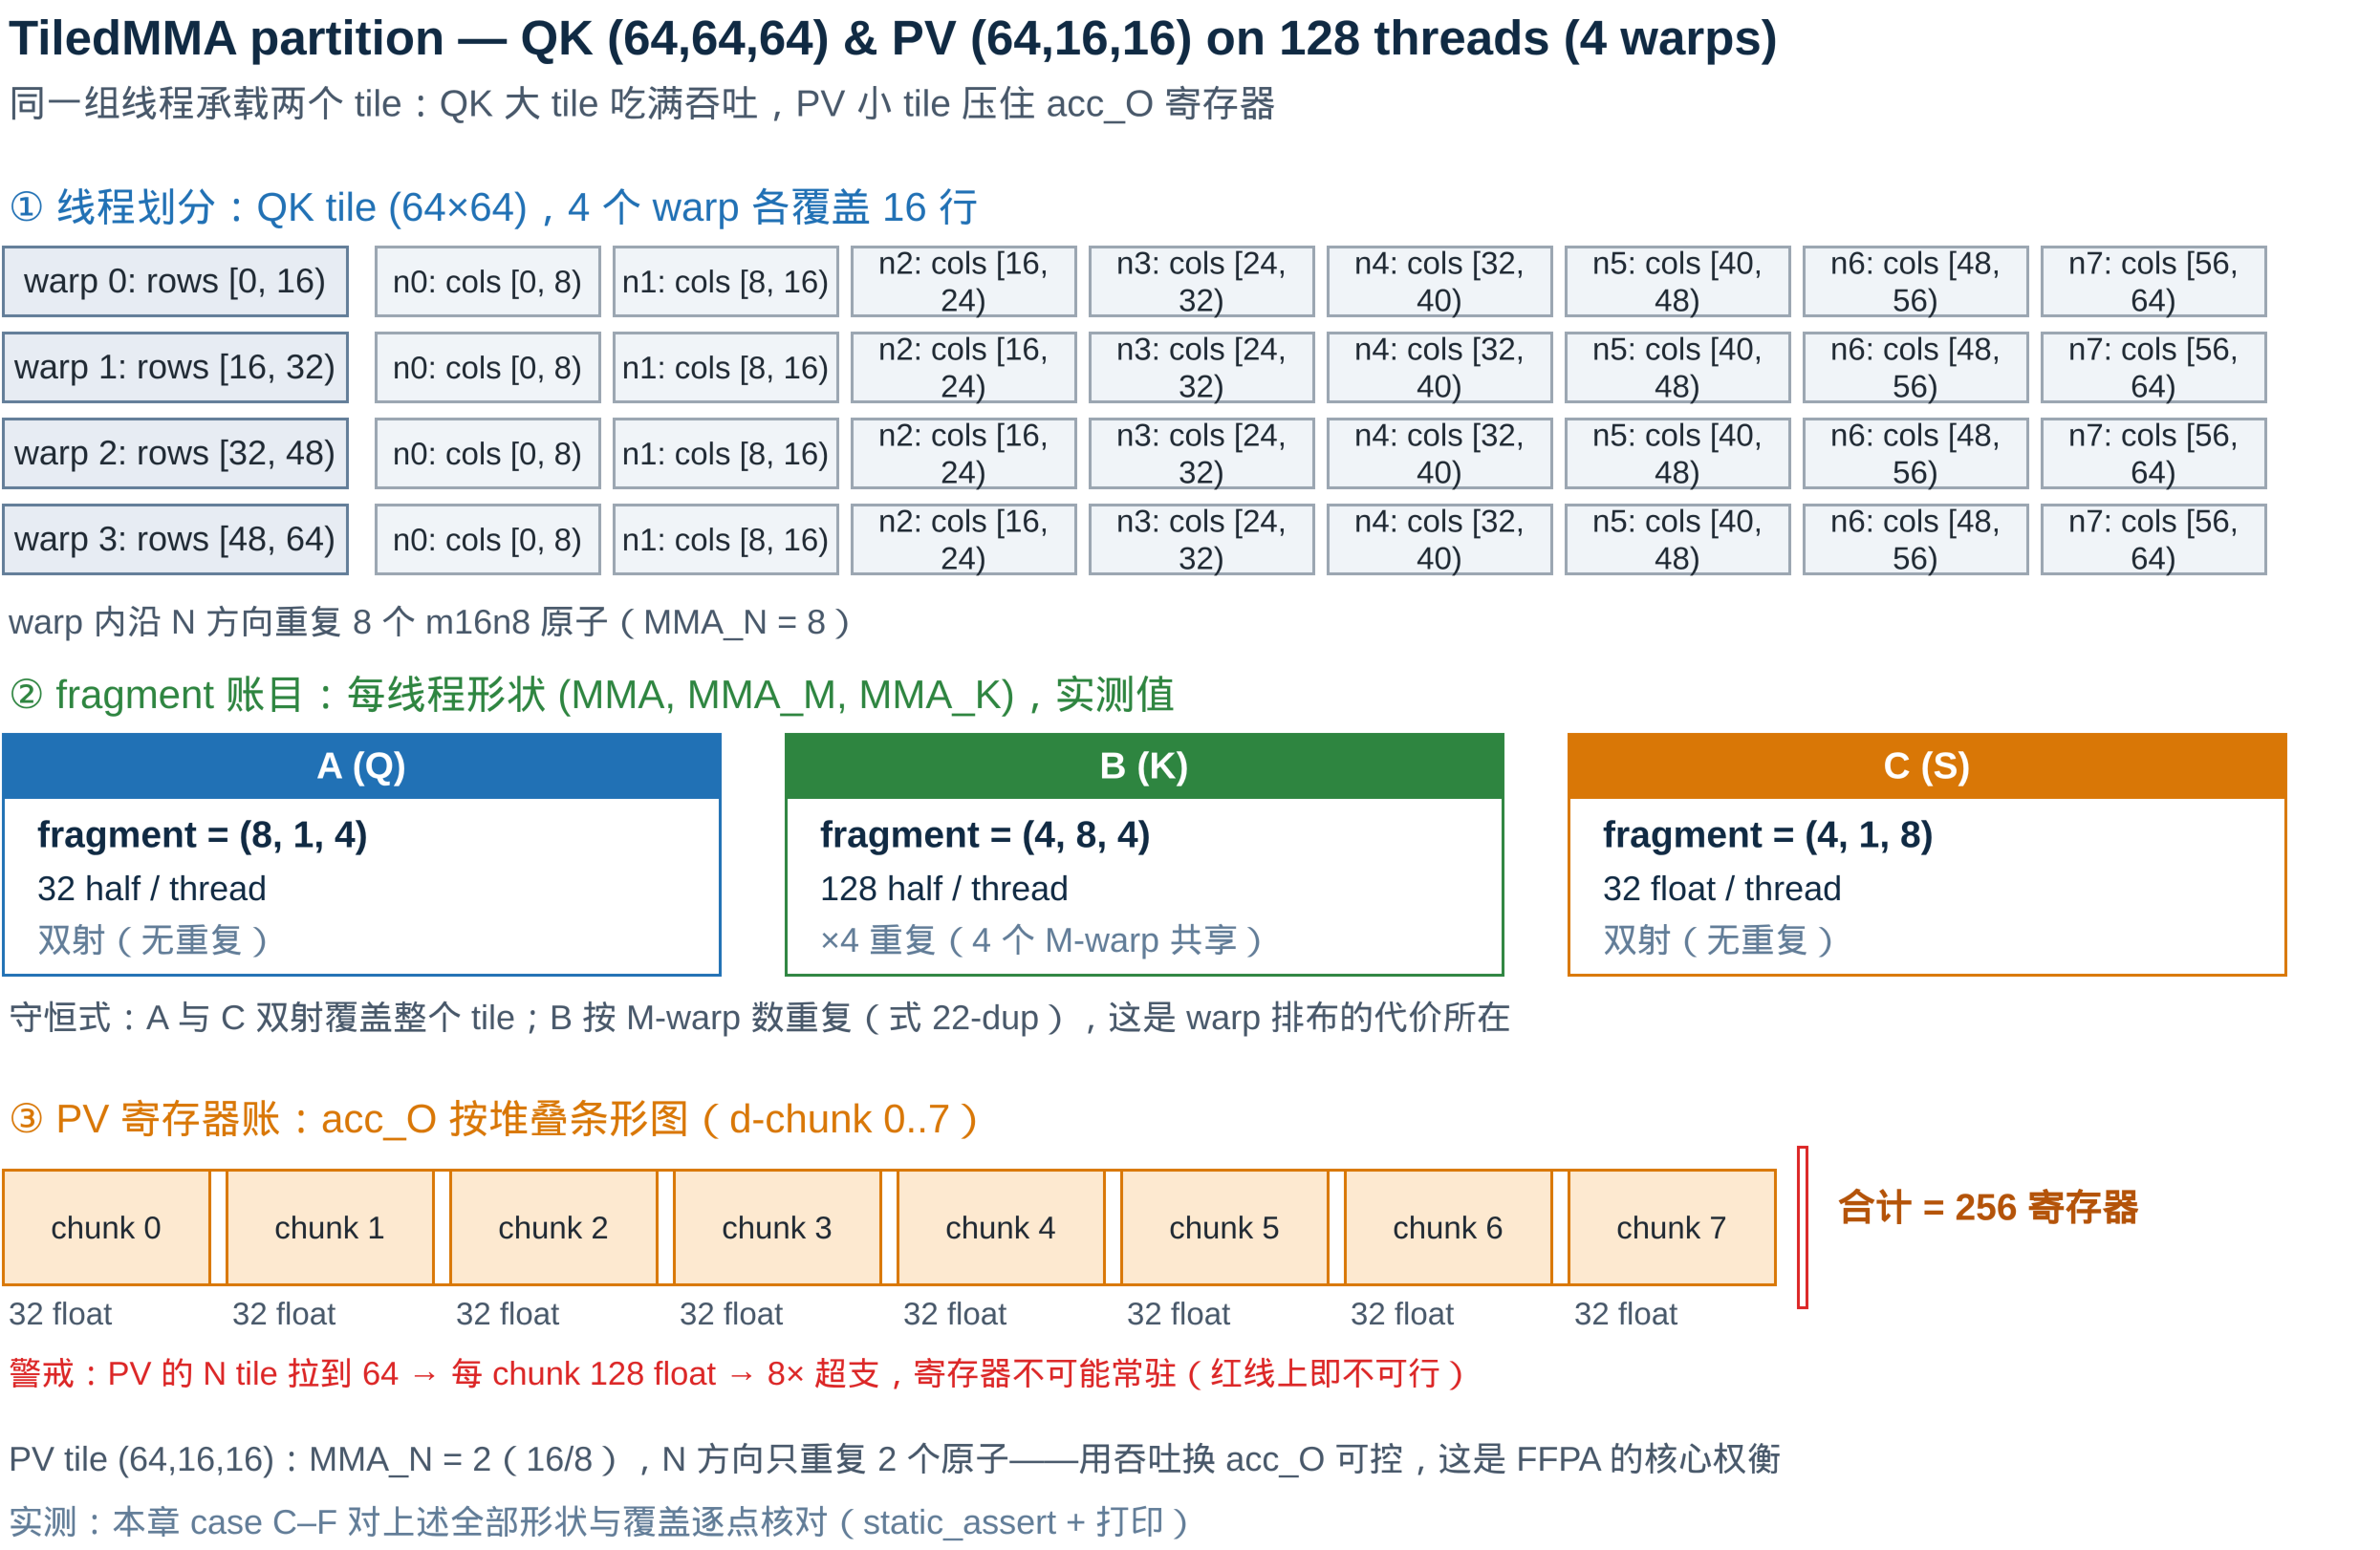
\includegraphics[width=0.92\textwidth]{figures/drawio/fig-22-1-tiledmma/fig-22-1.png}
\caption{TiledMMA partition：QK 的 $64\times64$ tile 上，4 个 warp 各覆盖
16 行，warp 内 N 方向重复 8 个原子；A/B/C 三种 fragment 的每线程形状与
重复因子（式~\eqref{eq:22-dup}）。下半部分是 PV 的 $(64,16,16)$ tile：
N 方向只重复 2 个原子，代价换来 per-call C 视图与拷贝粒度可控（8 个
d-chunk 各自拷回，常驻 acc\_O 256 寄存器不变；N tile 拉到 64 只是单次
调用的 C fragment 临时 4 倍）。本章测试 case~C--F
对全部形状与覆盖做了逐点核对。}
\label{fig:22-1}
\end{figure}

\begin{figure}[htbp]
\centering
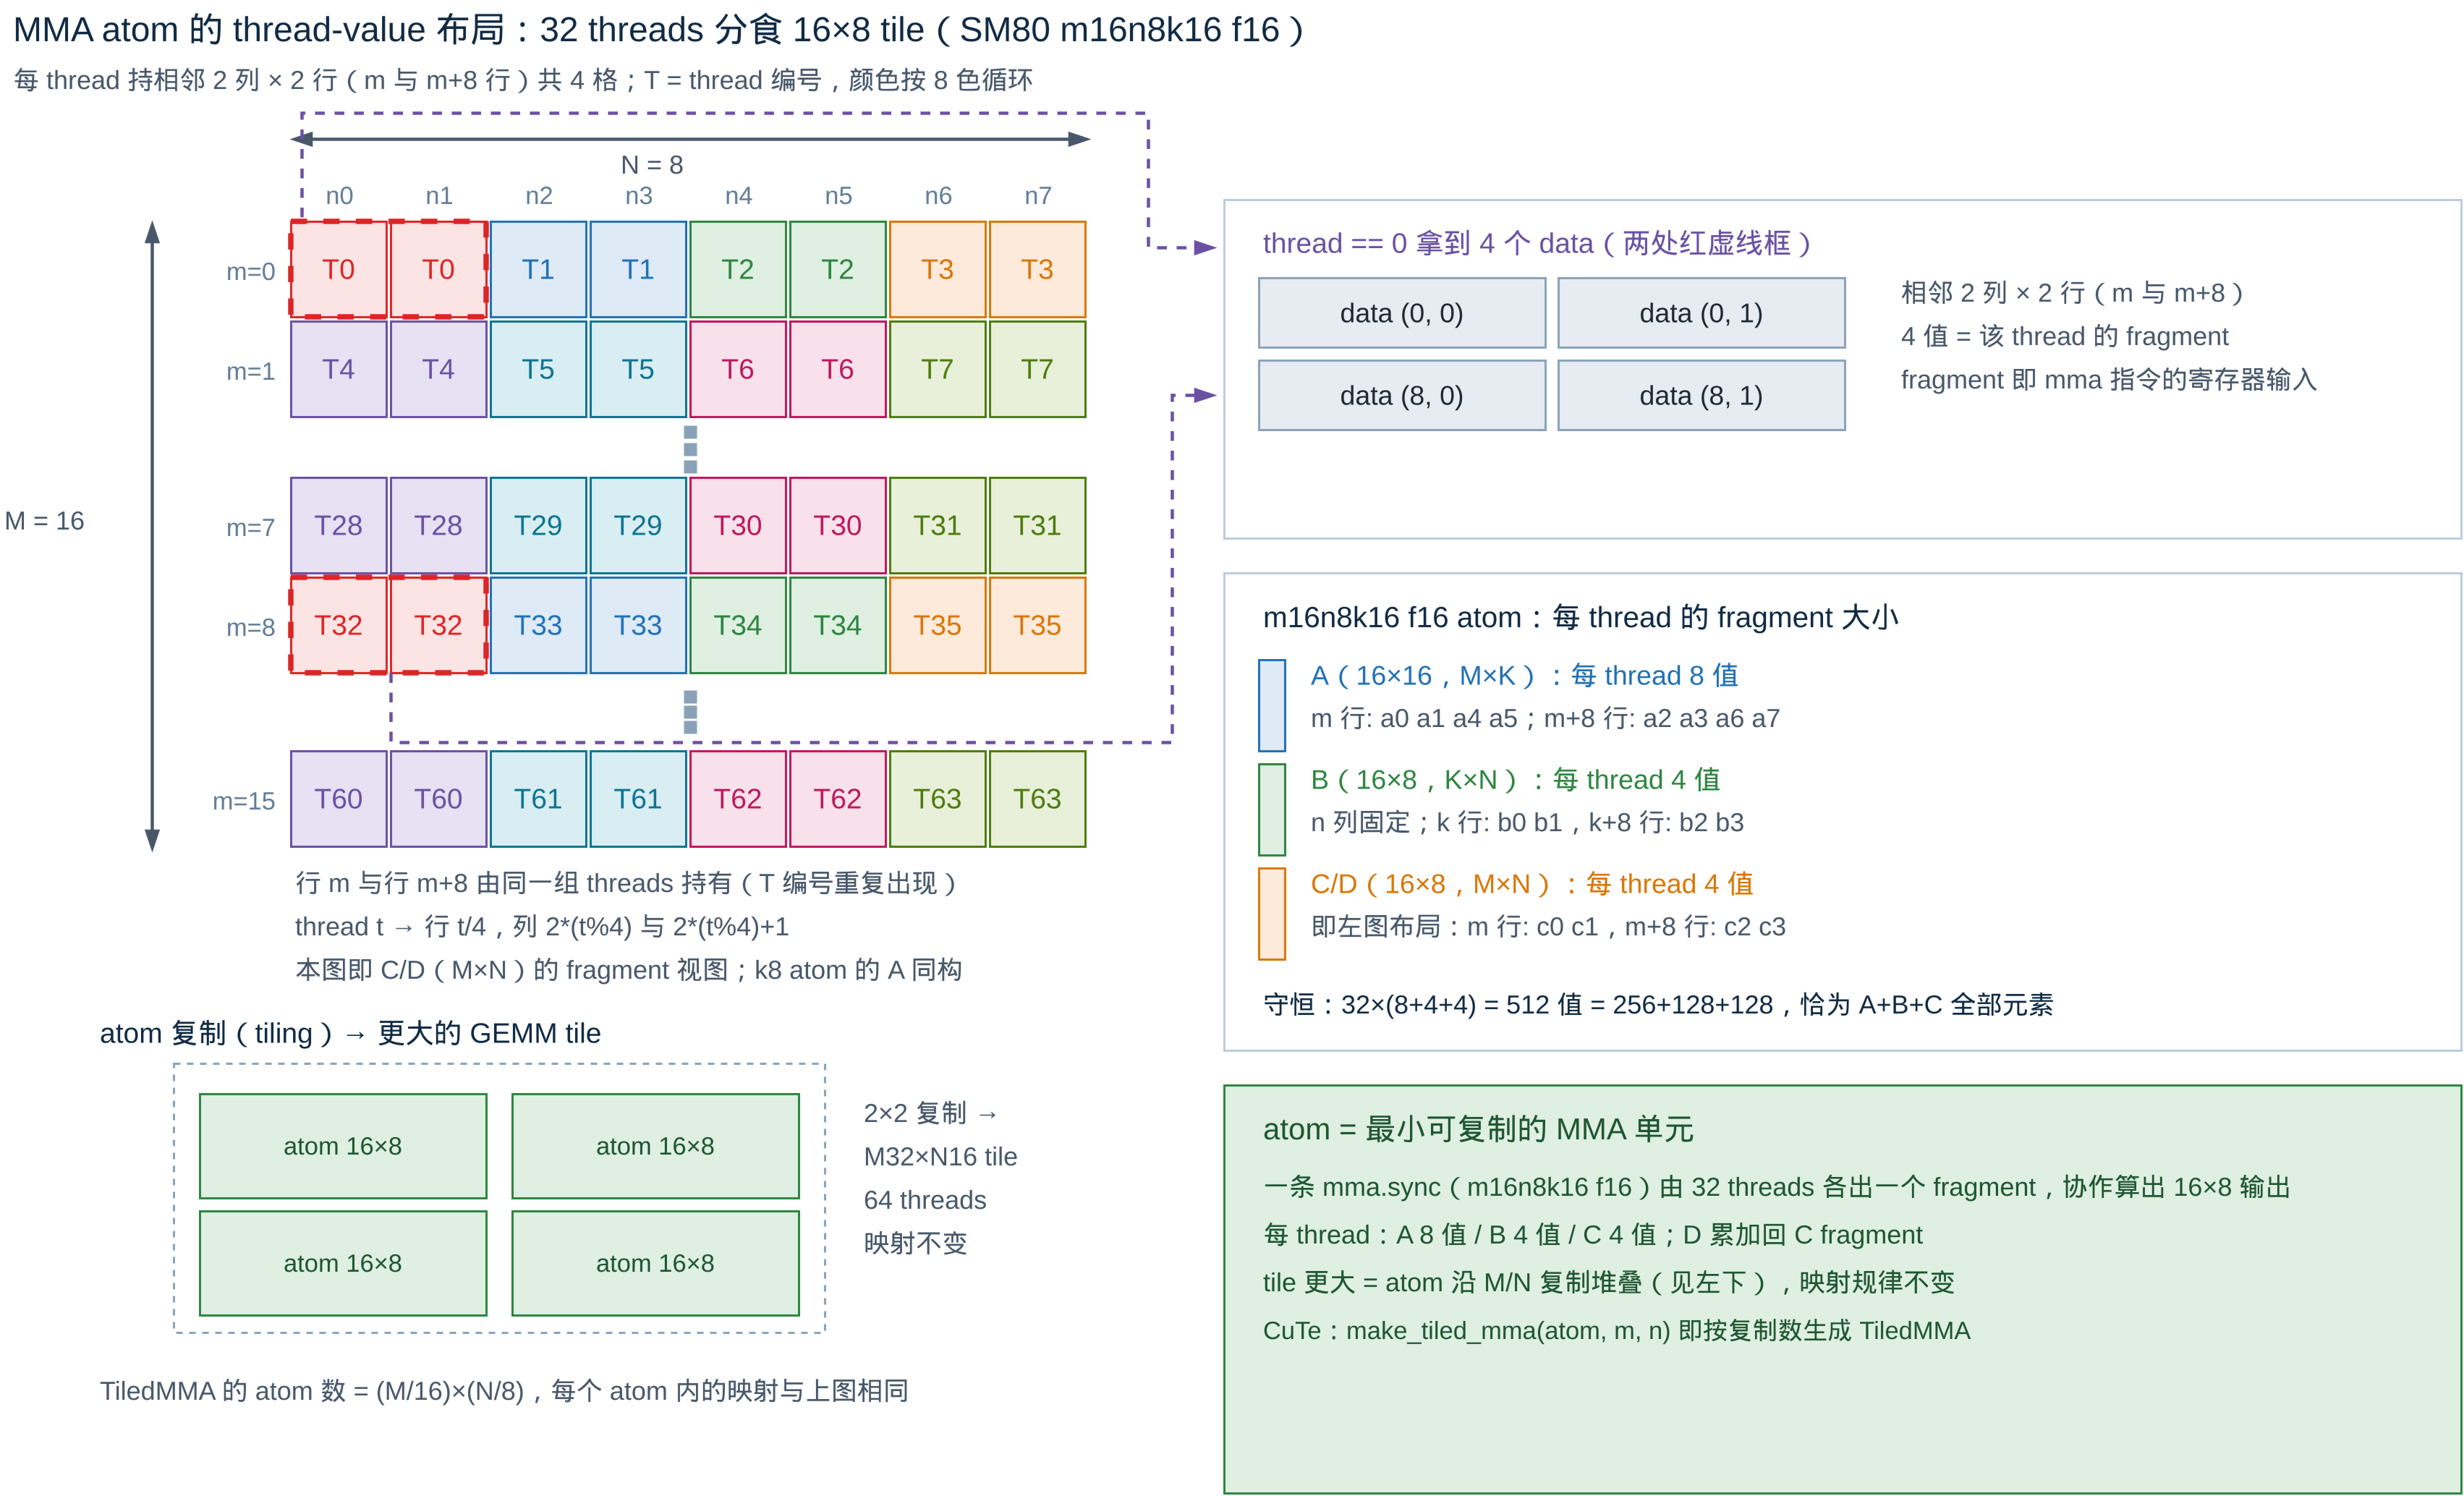
\includegraphics[width=0.95\textwidth]{figures/drawio/fig-22-2-mma-atom-fragments/fig-22-2.png}
\caption{m16n8k16 atom 的 C fragment thread-value 映射：thread $t$ 持行 $t/4$ 与 $t/4+8$、列 $2(t\bmod 4)$ 与 $2(t\bmod 4)+1$ 共 4 值——行 $m$ 与 $m+8$ 由同组线程重复持有。三个操作数每线程 A 8 值 / B 4 值 / C 4 值，守恒式 $32\times(8+4+4)=512$。更大的 tile 只是 atom 沿 M/N 的复制堆叠，thread-value 规律不变——\texttt{make\_\allowbreak{}tiled\_\allowbreak{}mma} 的构造基础。重建自 @竹熙佳处《写给大家看的 CuTe 教程：tiled mma》。}
\label{fig:22-2}
\end{figure}

\section{性能分析}

本章同样没有独立 bench：TiledMMA 的开销体现在它选择的 tile 形状上，端到端
数字在第~\ref{ch:19}、\ref{ch:26}~章（FFPA）与第~\ref{ch:24}~章（HGEMM）。
本节把「tile 选择」翻译成三条可计算的账。

\textbf{账一（寄存器）}：acc\_O $=kD_{\mathrm{chunks}}\times\mathrm{ThrLD}
\times\mathrm{MMA}_M\times\mathrm{MMA}_N\times\mathrm{Nrep}$（ThrLD 是单个
atom 每线程的 C 值数 $4$，Nrep 是 chunk 内 N 方向的重复数 $64/16=4$）
$=8\times4\times1\times2\times4=256$。PV 的
$\mathrm{MMA}_N = 2$（$16/8$）时每个 $64\times64$ d-chunk 每线程是 32 个
float；$D=512$ 时 $8$ 个 chunk 共 256 个寄存器。tile N=64 时单次 gemm 调用
的 C fragment 从 8 值涨到 32 值（4 倍），常驻 acc\_O（8 chunk $\times$ 32
$=$ 256 float）不变——超支的是每次调用的临时视图与 B fragment，不是
累加器。FFPA 注释「PV 保持小 tile」的算术依据正在于此：压的是每次调用的
临时开销，而非 acc\_O。

\textbf{账二（重复因子）}：B 的 fragment 按 M-warp 数重复（式~\eqref{eq:22-dup}）。
QK 用 $(4,1,1)$ 排布时 B 重复 4 倍（$4\times32=128$ 个 half/线程），
A 不重复；若改成 $(2,2,1)$（各方向 2 个 warp），A 与 B 各重复 2 倍——
总寄存器开销几乎不变，但 warp 覆盖的行会从 16 行变成 32 行。warp 排布的选择
因此是「谁重复」的问题，而不是「重复多少」的问题。

\textbf{账三（指令数）}：一次 TiledMMA 调用的指令数
$=\mathrm{MMA}_M\times\mathrm{MMA}_N\times\mathrm{MMA}_K$——注意这是
\emph{每线程（每 warp）}的条数。QK 的 $(1,8,4)=32$ 条是每个 warp 的量，
覆盖该 warp 的 $16\times64\times64$；4 个 warp 共 128 条才铺满 CTA 的
$64\times64\times64$——512 KFLOP/128 条，每条 $16\times8\times16$ 共
$4096$ FLOP（约 4.1 KFLOP）；PV 同口径：$(1,2,4)=8$ 条/warp 覆盖
$16\times16\times64$，CTA 的 $64\times16\times64$ 需 4 warp 共 32 条。
两个 tile 都让「每条 MMA 指令」吃满原子尺寸，没有浪费——因为它们都是从
$\mathrm{AtomShape}$ 出发、只用排布与 tile 尺寸做整数分块推出来的。

\textbf{口径说明}：本节所有数字都是 host 端类型推导的实测值（
\texttt{partition\_\allowbreak{}fragment\_\allowbreak{}*} 的形状），不含计时数据；FFPA 的
TFLOPS 对照见第~\ref{ch:19}~章的表与第~\ref{ch:26}~章的 kernel 分析。
还有一条引用纪律：ffpa\_attn.cuh L16--18 的头注释给出「SM120a
RTX PRO 5000：cuDNN SDPA 57.2 TFLOPS、FFPA TMA WS 110.7 TFLOPS（1.94x）」，
除法自洽（$110.7/57.2=1.94$），但设备口径是 \emph{RTX PRO 5000}（本机），
与 README 的 5090 口径不同——\textbf{引用这类比值时必须带上设备名}，
同一份代码在两块卡上的比值并不相等。

\section{常见坑}

\textbf{坑一：fragment 必须先清零/初始化。}
\texttt{partition\_\allowbreak{}fragment\_\allowbreak{}C} 返回的是「一块未定义的寄存器数组」的视图，
\emph{不会}置零。FFPA 里 \texttt{tCrS} 定义后立即 \texttt{clear(tCrS)}，
acc\_O 用显式循环清零（L173--176）。漏掉这一步的后果不是崩溃，而是把
未初始化寄存器当累加初值——编译器还可能把整个累加链折叠成垃圾值，
表现为「结果偶尔对、偶尔全错」。同理，被 \texttt{convert\_\allowbreak{}layout\_\allowbreak{}acc\_\allowbreak{}Aregs}
重解释的 $P$ 必须确保所有 32 个槽位都已被 softmax 写过。

\textbf{坑二：两个 TiledMMA 的 fragment 不能互换。}
QK 的 C fragment 是 $(4,1,8)$，PV 的 A fragment 是 $(8,1,4)$——形状、元素
类型（float/half）都不同。FFPA 的复用之所以成立，是因为它做了
\emph{类型转换 $+$ 布局重解释}两步（\texttt{convert\_\allowbreak{}type} $+$
\texttt{convert\_\allowbreak{}layout\_\allowbreak{}acc\_\allowbreak{}Aregs}），且只对 m16n8k16 这一族成立。
把 C 直接喂给 PV 是经典的静默错位。

\textbf{坑三：tile 必须是原子的整数倍，warp 排布必须与线程数自洽。}
$\mathrm{perm\_M}$ 不是 $16$ 的倍数、或 $\mathrm{ThrM}\times 32$ 与
\texttt{blockDim} 不一致时，partition 会产生多余/缺失的 remainder mode
（编译期静态断言或运行期越界）。判据：\texttt{size(mma)} 是线程数的权威，
用它来配 \texttt{dim3 block\allowbreak{}(size\allowbreak{}(mma))}。

\textbf{坑四：\texttt{get\_slice} 的坐标是 $(\mathrm{ThrV},(\mathrm{ThrM},
\mathrm{ThrN/K}))$ 三层，不是「warp 内 lane $+$ 全局 warp」两层。}
FFPA 的 $128$ 线程排布是 $(\mathrm{ThrV}=32,\mathrm{ThrM}=4)$，因此
线程 $t$ 的行带是 $16\lfloor t/32\rfloor$——把 $\mathrm{ThrM}$ 当成
「线程号对 4 取模」会得到完全错误的 warp 映射（本章测试 case~E 专门核对
这条）。

\textbf{坑五：\texttt{partition\_\allowbreak{}fragment\_\allowbreak{}A} 的输入决定 fragment 的
MMAK 大小，但不改变 atom 约定。}
QK 的 A 在 $(64,64)$ 上是 $(8,1,4)$，在 $(64,16)$ 上就是 $(8,1,1)$；
$\mathrm{MMA}_K$ 随输入 K 长度变化。写循环时要用
\texttt{size\allowbreak{}<2>\allowbreak{}(fragment)} 作为 K 循环上界（第~\ref{ch:21}~章 kernel 的
\texttt{num\_k\_steps} 就是这么来的），不要写死。

\textbf{坑六：C fragment 的「行列」不是直觉顺序。}
$(4,1,8)$ 的 4 个 float 对应「2 行 $\times$ 2 列」，同一个 lane 的第 0、1 个
元素在同一行相邻两列，第 2、3 个在 $+8$ 行处。想按 (row, col) 遍历必须先做
\texttt{convert\_\allowbreak{}layout\_\allowbreak{}acc\_\allowbreak{}rowcol}（L2315--2333 推导）；直接用
\texttt{fragment\allowbreak{}(idx)} 当矩阵元素是最常见的读错方式。

\section{面试要点速查}

\textbf{Q1：MMA\_Atom 与 TiledMMA 的区别？}\\
A：MMA\_Atom 是一条指令的抽象（Shape\_MNK $+$ 三份 TV layout $+$ ThrID）；
TiledMMA 是「把原子铺满一个 tile」的类型，多出 warp 排布与 tile 尺寸两个
参数，并提供 \texttt{partition\_\allowbreak{}fragment\_\allowbreak{}*}。

\textbf{Q2：\texttt{make\_\allowbreak{}tiled\_\allowbreak{}mma} 的第二个、第三个参数分别是什么？}\\
A：第二个是 warp 排布（\texttt{Atom\allowbreak{}Layout\allowbreak{}MNK}，决定 \texttt{Thr\allowbreak{}M/\allowbreak{}Thr\allowbreak{}N/\allowbreak{}Thr\allowbreak{}K}
与重复因子），第三个是目标 tile 尺寸（\texttt{Permutation\allowbreak{}MNK}，含 K）。
FFPA：排布 $(4,1,1)$，tile $(64,64,16)$ 与 $(64,16,16)$。

\textbf{Q3：fragment 的三个 mode 是什么？}\\
A：$(\mathrm{MMA}, \mathrm{MMA}_M, \mathrm{MMA}_K)$——每个原子的值数、
M 方向原子重复、K 方向原子重复（C 的第三 mode 是
$\mathrm{MMA}_N$）。它们是式~\eqref{eq:22-thrfrg-4} 第 (4) 步之后的余量。

\textbf{Q4：为什么 A 的 fragment 有时会重复？}\\
A：warp 排布如果在 N 方向有分片，不同 N-warp 需要同一份 A，于是 A 被
重复持有（重复因子 $=$ N-warp 数）；B 同理（因子 $=$ M-warp 数）。
式~\eqref{eq:22-dup}。

\textbf{Q5：\texttt{get\_\allowbreak{}slice\allowbreak{}(t)} 内部发生了什么？}\\
A：把整数 $t$ 按 \texttt{Thr\allowbreak{}Layout\allowbreak{}VMNK} 分解成
$(\mathrm{ThrV},(\mathrm{ThrM},\mathrm{ThrN}),\mathrm{ThrK})$，得到一个
「只属于该线程」的 ThrMMA，后续 partition 都基于它。

\textbf{Q6：QK 与 PV 为什么要用两个 TiledMMA？}\\
A：目标不同。QK 要一次覆盖整个 $S$（N $=64$）省循环；PV 的 N 直接决定
acc\_O 的寄存器数，必须小。两者共享同一套 128 线程排布，fragment 通过
类型转换 $+$ 布局重解释衔接。

\textbf{Q7：\texttt{tile\_\allowbreak{}size\allowbreak{}<I>\allowbreak{}(mma)} 有什么用？}\\
A：它是 TiledMMA 对外的尺寸接口，也是 \texttt{make\_\allowbreak{}tiled\_\allowbreak{}copy\_\allowbreak{}A/\allowbreak{}B/\allowbreak{}C}
推导 S$\to$R 拷贝 tiler 的来源（第~\ref{ch:21}~章式~(21-mtca)）——
TiledMMA 与 TiledCopy 通过它解耦：改 tile 不影响拷贝代码。

\textbf{Q8：tile 的 N 尺寸调节什么？}\\
A：单次调用 C fragment 每线程元素数 $=\mathrm{MMA}\times\mathrm{MMA}_M\times
\mathrm{MMA}_N$，而 $\mathrm{MMA}_N = \mathrm{tile}_N/\mathrm{atom}_N$——
tile N 增大时 per-call C 视图与 B fragment 随之线性增长，S$\to$R 拷贝
粒度变粗；常驻 acc\_O（$D=512$ 时 256 个寄存器）不变，PV 因此取
$\mathrm{tile}_N=16$（$64\times16\times16$）。

\section{最小测试与动手实验}

测试文件：\texttt{book/\allowbreak{}tests/\allowbreak{}ch22\_\allowbreak{}tiled\_\allowbreak{}mma.cu}（host-only：只做类型与
partition 断言，不启动 kernel；直接 include
\texttt{.\allowbreak{}.\allowbreak{}/\allowbreak{}.\allowbreak{}.\allowbreak{}/\allowbreak{}ffpa\_\allowbreak{}attn.\allowbreak{}cuh} 以核对真实的 traits）。六个 case：

\begin{itemize}
  \item \textbf{A 原子 fragment 公式}：对
        \texttt{SM80\_\allowbreak{}16x8x16\_\allowbreak{}F32\allowbreak{}F16\allowbreak{}F16\allowbreak{}F32\_\allowbreak{}TN} 的 A/B/C 三个 layout，
        逐 lane、逐值核对手推公式式~\eqref{eq:22-atom-a}--\eqref{eq:22-atom-c}
        （$32\times8$、$32\times4$、$32\times4$ 个断言）；
  \item \textbf{B tile\_size 与线程数}：QK/PV 的 \texttt{tile\_size} 为
        $(64,64,16)/(64,16,16)$、\texttt{size(mma)}$=128$；对象
        \texttt{FFPAAttn\allowbreak{}Split\allowbreak{}DCu\allowbreak{}Te\allowbreak{}Traits\allowbreak{}<512>}
        并与手写的
        \texttt{make\_\allowbreak{}tiled\_\allowbreak{}mma} 构造做类型一致性检查；
  \item \textbf{C fragment 形状}：QK 在 $(64,64)$ 上 A/B/C 每线程
        $(8,1,4)/(4,8,4)/(4,1,8)$，PV 为 $(8,1,4)/(4,2,1)/(4,1,8)$；
        逐项核对元素数；
  \item \textbf{D 守恒与重复因子}：C 的覆盖是双射（$128\times32=4096=
        64\times64$）且 A 也是；B 恰好 4 倍重复（每元素被 4 个
        (线程, 值) 对覆盖）；
  \item \textbf{E warp 边界}：QK 的 C fragment 逐线程回投坐标，四个 warp 的
        行带为 $[0,16),[16,32),[32,48),[48,64)$，互不重叠；
  \item \textbf{F PV 的 acc\_O 账目}：
        \texttt{partition\_\allowbreak{}fragment\_\allowbreak{}C\allowbreak{}(tiled\_\allowbreak{}mma\_\allowbreak{}pv,\allowbreak{} Shape\allowbreak{}<\_\allowbreak{},\allowbreak{}64,\allowbreak{}\_\allowbreak{}64>\{\})}
        每线程 32 个值，$\times$ 8 个 d-chunk（$D=512$）$=256$ 个寄存器——
        与源码注释的寄存器压力说法互证；并核对 PV 的 C 覆盖
        （$64\times16$ 双射）。
\end{itemize}

运行命令：

\begin{lstlisting}[style=console]
cd kernels/interview/book/tests
CUDA_VISIBLE_DEVICES=6 ./build_tests.sh --arch sm_120a --ch ch22
\end{lstlisting}

预期输出（本机 RTX PRO 5000，CUDA 13.2，CUTLASS v4.6.1，2026-09-11 实测）：

\begin{lstlisting}[style=console]
ch22 CuTe TiledMMA & fragments (host-only, no kernel launch)
PASS case A MMA atom fragment layouts (m16n8k16): mismatches=0 (519 checks)
PASS case B FFPA traits tile_size & thread count: mismatches=0 (14 checks)
PASS case C partition_fragment shapes QK/PV: mismatches=0 (12 checks)
PASS case D conservation & B duplication factor: mismatches=0 (4 checks)
PASS case E warp row bands & cross-warp boundary: mismatches=0 (4360 checks)
PASS case F PV acc_O register budget & coverage: mismatches=0 (136 checks)
ALL OK
\end{lstlisting}

动手实验：

\begin{enumerate}
  \item 把 case~C 的 PV mma 的 tile 从 \texttt{Tile\allowbreak{}<64,\allowbreak{}16,\allowbreak{}16>} 改成
        \texttt{Tile\allowbreak{}<64,\allowbreak{}32,\allowbreak{}16>}，观察 fragment 的 $\mathrm{MMA}_N$ 从 2 变
        4、单次调用的 C 视图从 8 涨到 16 个值，而单个 d-chunk 的 acc\_O
        仍是 32——亲手体验「tile N 调节 per-call C 视图与拷贝粒度」；
  \item 把 QK 的 warp 排布从 \texttt{Layout\allowbreak{}<Shape\allowbreak{}<\_\allowbreak{},\allowbreak{}4,\allowbreak{}\_\allowbreak{},\allowbreak{}\_\allowbreak{}>>} 改成
        \texttt{Layout\allowbreak{}<Shape\allowbreak{}<\_\allowbreak{},\allowbreak{}2,\allowbreak{}\_\allowbreak{}2,\allowbreak{}\_\allowbreak{}>>}（$2\times2$ 网格），观察
        A/B 的重复因子与 warp 行带如何变化（case~D/E 的断言会同时失效，
        这正是要看的现象）；
  \item 把 case~A 的 lane 换成 $32+k$ 或把值编号顺序反转，确认断言能立刻
        抓到错误——用来理解「formula-driven 测试」与「只比形状」的差别。
\end{enumerate}

\section*{延伸阅读}

\begin{itemize}
  \item @竹熙佳处《写给大家看的 CuTe 教程：Tiled MMA》，
        \url{https://zhuanlan.zhihu.com/p/1937145378446226159}
        （本计划的 ch22 主参考；素材清单标注「待核」，本章全部结论以
        CUTLASS v4.6.1 头文件实测为准）；
  \item @reed《cute 之 MMA 抽象》，
        \url{https://zhuanlan.zhihu.com/p/663092747}
        （MMA\_Atom/MMA\_Traits 的设计动机与历史，读 3.1--3.2 节时对照）；
  \item @可怕的杰瑞《Cute TiledMMA 简单理解》，
        \url{https://zhuanlan.zhihu.com/p/1991908850132088026}
        （用可编译的最小例子演示 make\_tiled\_mma 的三个参数，
        与本章 case~B 的实验同构；续篇
        \url{https://zhuanlan.zhihu.com/p/1992328297888126320}）；
  \item @水木皇工仔《基于 CuTe 理解 swizzle, LDSM, MMA》，
        \url{https://zhuanlan.zhihu.com/p/934430036}
        （把 LDSM 的 lane 映射与 MMA fragment 放在一起推，与第~\ref{ch:21}~章
        case~D、本章 case~A 互补）。
\end{itemize}


% ch23-cute-swizzle-tma.tex — 骨架（RFC-0.3），撰写任务见 RFC.md F4
\chapter{CuTe（四）：Swizzle 与 TMA}\label{ch:23}

本章待撰写。源码区间：新写，对照 SW128 atom 用法；执行卡片：RFC.md F4；章节模板：\texttt{chapters/\_template.tex}（10 节结构 + DoD 八条）。

% ch24-cute-hgemm.tex — CuTe 应用（一）：HGEMM（RFC-F，2026-09-11）
% \url 由 book.tex 的 hyperref 提供；单章独立编译时降级为可断行的 \ttfamily
% （逐字符插入 \allowbreak，避免长 URL 造成 Overfull \hbox）
\makeatletter
\providecommand{\urlchbrk}[1]{\@tfor\next:=#1\do{\next\allowbreak}}
\makeatother
\providecommand{\url}[1]{{\ttfamily\urlchbrk{#1}}}
\chapter{CuTe 应用（一）：HGEMM}\label{ch:24}

\section{本章导读}

第~\ref{ch:11}、\ref{ch:12}~章用两条不同的路把同一个 HGEMM 写了两遍：一条是
「手写 MMA PTX $+$ 手算 smem 地址」的 Phase~7b，另一条是「手写 XOR swizzle $+$
寄存器双缓冲」的 Phase~7b-3。两条路都跑到了 122\,TFLOPS 量级，但代价是同一组
「形状与步长」的事实被反复重写：\texttt{ldmatrix} 的 lane 映射、swizzle 的
XOR 掩码、epilogue 的 \texttt{\_\_shfl\_sync} 编排，每一处都要人工保证与其余
四处的地址算术一致。本章把同一个 kernel 交给 CuTe 重写一遍——Phase~7c 的
\texttt{hgemm\_mma\_stages\_tn\_cute}，并在最后用一张\textbf{对照表}
（图~\ref{fig:24-1}）把两条路逐项摆开。

\textbf{前置章节}：第~\ref{ch:11}~章（\texttt{mma.sync.m16n8k16} 与
\texttt{ldmatrix}）、第~\ref{ch:12}~章（XOR swizzle 与寄存器双缓冲）、
第~\ref{ch:20}--\ref{ch:23}~章（Layout 代数 / Tensor 与 TiledCopy / TiledMMA /
Swizzle 与 TMA）。本章是 Part~IV 的第一章「应用篇」，只用到前四章已经介绍过的
四个抽象：\texttt{Layout}、\texttt{Tensor}、\texttt{TiledCopy}、
\texttt{TiledMMA}。

\textbf{源码区间}：hgemm.cuh~L718--1427——Phase~7c 头注释（L718--778）、
宏块 \texttt{NOTES\_V2\_ENABLE\_CUTE}（L779--1427）内的 kernel
\texttt{hgemm\_mma\_stages\_tn\_cute}（L821 起）与 launch wrapper
\texttt{launch\_hgemm\_mma\_stages\_tn\_cute}（L1216 起）。\textbf{编译宏}：
\texttt{NOTES\_V2\_ENABLE\_CUTE}（需要 CUTLASS 头文件；sm80 及以上均可编）。
\textbf{架构}：本章 kernel 只用 SM80 时代的 \texttt{cp.async} $+$
\texttt{mma.sync} $+$ \texttt{ldmatrix}，本机 sm\_120a 可实测。

配套最小测试 \texttt{book/tests/ch24\_hgemm\_cute.cu}：两组配置
（\texttt{kAccF32=false}、$B_N=256$ 与 \texttt{kAccF32=true}、$B_N=128$）对 CPU
fp64 参考做正确性判定；本章的实测数字全部来自该测试与 \texttt{ptxas -v}，
端到端性能对照见 \texttt{.tmp/book-bench}（其它章）。预计篇幅约 12 页。

\section{问题与动机}

先把第~\ref{ch:11}、\ref{ch:12}~章的代码量摆出来（只统计代码行，去掉纯注释
与空行；统计口径见第~\ref{sec:24-minitest}~节）：

\begin{itemize}
  \item Phase~7b \texttt{hgemm\_mma\_stages\_tn}（hgemm.cuh~L129--397）：
        \textbf{147 行}；
  \item Phase~7b-3 \texttt{hgemm\_mma\_stages\_tn\_swizzle}
        （hgemm.cuh~L434--716）：\textbf{231 行}；
  \item Phase~7c \texttt{hgemm\_mma\_stages\_tn\_cute}
        （hgemm.cuh~L821--1196）：\textbf{118 行}，再加 launch wrapper
        （L1216--1427）\textbf{86 行}。
\end{itemize}

手写版与 CuTe 版的「行数比」并不悬殊（231 对 204），但\textbf{代码的性质变了}。
手写版里出现的是地址表达式与内联 PTX：

\begin{verbatim}
int lane_smem_a_m = warp_m * (kMmaM * kValTileM) + i * kMmaM + lane_id % 16;
int lane_smem_a_k = k_step * kMmaK + (lane_id / 16) * 8;
uint32_t lane_smem_a_ptr = smem_a_base_ptr +
    (stage * BM * BK + lane_smem_a_m * BK +
     swizzle<64>(lane_smem_a_m, lane_smem_a_k)) * sizeof(half);
LDMATRIX_X4(RA[i][0], RA[i][1], RA[i][2], RA[i][3], lane_smem_a_ptr);
\end{verbatim}

CuTe 版里出现的是\textbf{声明}与\textbf{分区}：

\begin{verbatim}
auto sA = make_tensor(make_smem_ptr(Ashm), SmemLayoutA{});
auto tAsA = s2r_thr_copy_a.partition_S(sA);
auto tCrA_view = s2r_thr_copy_a.retile_D(tCrA);
cute::copy(s2r_tiled_copy_a, tAsA(_, _, k_step_next, ismem_read),
           tCrA_view(_, _, k_step_next));
\end{verbatim}

前者把「\texttt{lane} 到 smem 地址」的公式写死在 kernel 里，改一个 tile 尺寸
就要把公式推倒重来；后者把同一件事表达成「\texttt{sA} 的布局是
\texttt{SmemLayoutA}」「\texttt{s2r\_thr\_copy\_a} 把 sA 按线程切分」两句
声明，地址算术由编译器（类型系统）展开。这就是第~\ref{ch:20}--\ref{ch:23}~章
铺垫四章的回报：\textbf{把布局从代码里提出来，变成一等公民}。

本章要回答三个问题：这 118 行的 kernel 本体究竟做了什么？launch wrapper 的 86
行「类型实例化」在配置什么？以及——最重要的——\textbf{哪些东西 CuTe 替你做了，
哪些东西仍然要你自己做}？第三个问题决定了这套工具的能力边界，也是
图~\ref{fig:24-1} 对照表要回答的。

\section{数学原理}

\subsection{问题定义与 TN 布局}

本章沿用第~\ref{ch:11}~章的 TN 约定：
$C[M,N] = A[M,K]\times B^{\mathsf T}[N,K]$，其中 $A$、$B^{\mathsf T}$ 都是
row-major（\texttt{A[m][k]}、\texttt{Bt[n][k]}）。写成求和形式：

\begin{equation}
  C_{m,n} \;=\; \sum_{k=0}^{K-1} A_{m,k}\, B_{n,k},
  \label{eq:24-tn}
\end{equation}

注意式~\eqref{eq:24-tn} 里 $B$ 的索引是 $(n,k)$——这正是 TN 的含义：MMA 指令
\texttt{mma.sync.aligned.m16n8k16.row.col} 要求 A 为 row-major、B 在 GEMM
语义下为 col-major，而 col-major 的 $B[K,N]$ 与 row-major 的
$B^{\mathsf T}[N,K]$ 是同一块内存。\textbf{这是本章第一个坑}：调用方必须自己
把 $B$ 转置后传入（最小测试里由 host 侧转置完成，见
第~\ref{sec:24-minitest}~节）。

\subsection{Tile 金字塔与默认推导}

设 CTA 级 tile 为 $B_M\times B_N\times B_K$，网格为
$\bigl(\lceil N/B_N\rceil,\lceil M/B_M\rceil\bigr)$。Phase~7c 的默认配置：

\begin{equation}
  B_M=128,\qquad
  B_N=\begin{cases}256, & \text{F16 累加}\\ 128, & \text{F32 累加}\end{cases},
  \qquad B_K=32,\qquad k_{\mathrm{stage}}=2 .
  \label{eq:24-tile}
\end{equation}

$B_N$ 随累加精度切换是\textbf{经验性}的：F32 累加器每个元素占 4 字节，寄存器
压力翻倍，$128\times256$ 的 C tile 在 128 线程下是
$128\cdot256/128=256$ 个 float 累加器——已经超过可用寄存器的一半，会溢出到
local memory。第~\ref{sec:24-kaogu}~节用 \texttt{ptxas -v} 实测核对这条注释。
$B_K=32$ 与 $k_{\mathrm{stage}}=2$ 一起决定了 smem 占用：

\begin{equation}
  \underbrace{128\cdot32\cdot2}_{\text{A：}B_M B_K k_{\mathrm{stage}}}
  +\underbrace{256\cdot32\cdot2}_{\text{B：}B_N B_K k_{\mathrm{stage}}}
  = 24576\ \text{个 half} = 48\,\text{KiB},
  \label{eq:24-smem}
\end{equation}

也就是说这个 kernel 落在「一个 CTA 占 48\,KiB smem」的档位上（本机 PRO~5000
每 SM 228\,KiB，理论上限更高，但占用率还要受寄存器与 block 数约束）。

\subsection{MMA atom 与 EURepeat}

MMA atom 取 SM80 的 \texttt{m16n8k16}，A/B 均为 fp16、累加器可选 fp16 或 fp32：

\begin{center}
\begin{tabular}{lll}
\toprule
项 & F16 累加 & F32 累加 \\
\midrule
PTX 形状 & \texttt{m16n8k16} & \texttt{m16n8k16} \\
CuTe atom & \texttt{SM80\_16x8x16\_F16F16F16F16\_TN}
           & \texttt{SM80\_16x8x16\_F32F16F16F32\_TN} \\
C 累加器 & 2 个 \texttt{u32}（4 个 half） & 4 个 float \\
\bottomrule
\end{tabular}
\end{center}

两种 atom 的 A/B fragment 布局完全相同（这也是选它们做对照的前提），差别只在
C 累加器：F16 累加把 4 个 half 塞进 2 个寄存器，F32 累加用 4 个寄存器。launch
wrapper 用 \texttt{std::conditional\_t} 一次选出原子，再由 EURepeat 推出逻辑
tile：

\begin{equation}
  \texttt{kMmaPM}=2\times16=32,\quad
  \texttt{kMmaPN}=2\times8=32,\quad
  \texttt{kMmaPK}=1\times16=16 ,
  \label{eq:24-tile-mma}
\end{equation}

即 EURepeat$(M,N,K)=(2,2,1)$、逻辑 MMA tile 为 $32\times32\times16$，线程数
$\mathrm{size}(\texttt{MMA})=4\ \text{warps}\times(2\times2)=128$。
$B_K=32$ 相对 \texttt{kMmaPK}$=16$ 的倍数即 K 方向的切片数：

\begin{equation}
  n_{k\text{-step}} \;=\; \frac{B_K}{\texttt{kMmaPK}} \;=\; \frac{32}{16} \;=\; 2,
  \label{eq:24-kstep}
\end{equation}

这就是 kernel 里 \texttt{num\_k\_steps = size<2>(tCrA)} 的来历——它不是一个
magic number，而是「K-mode 的 extent」被 CuTe 从类型里读出来的结果。

\subsection{流水线的不变量}

$k_{\mathrm{stage}}=2$ 的 \texttt{cp.async} 流水用三个计数器描述状态：
\texttt{itile\_to\_read}（下一个要发起的 K-tile 序号）、\texttt{ismem\_read}
（当前计算消费的 stage 槽位）、\texttt{ismem\_write}（下一个要写入的槽位）。
预取填满 $k_{\mathrm{stage}}-1=1$ 个槽位后，主循环的每个 K-tile 里做三件事：
用当前 stage 算 MMA、发起下一个 K-tile 的 G$\to$S、在最后一个 k\_step 处
\texttt{cp\_async\_wait<kStage-2>()} 后翻转 \texttt{ismem\_read}。不变量是

\begin{equation}
  \#\{\text{已提交未等待}\} \;\le\; k_{\mathrm{stage}}-1 ,
  \label{eq:24-inflight}
\end{equation}

即最多一个 tile 在飞：这是 $k_{\mathrm{stage}}=2$ 时 \texttt{wait} 的语义
（\texttt{cp\_async\_wait<N>} 等待「不超过 $N$ 组未完成」）。$k_{\mathrm{stage}}$
加到 3、4 时同样的代码自动放行更多在飞 tile——循环体本身不需要改。

\subsection{Epilogue 的数据量核算}

C 怎么从寄存器回到 gmem？Phase~7c 的答案是「先落 smem，再由 smem 宽写」。
C scratchpad 复用当前 A stage 的空间，容量对齐关系是

\begin{equation}
  \underbrace{32\cdot32\cdot4}_{\text{C scratchpad}}
  \;=\;
  \underbrace{128\cdot32}_{\text{一个 A stage}}
  \;=\; 4096 ,
  \label{eq:24-cpipe}
\end{equation}

恰好相等，所以 kernel 里可以写
\texttt{sC = make\_tensor(sA(\_,\_,ismem\_read).data(), SmemLayoutC\{\})}——只别名
\textbf{一个} A stage，而不是整块双缓冲。这条等式由 launch wrapper 的
\texttt{static\_assert} 在编译期守住；改 $B_K$ 或 \texttt{kSmemLayoutCBatch}
时它会立刻报错，而不是在运行时静默越界。

\section{设计与实现}

\subsection{kernel 签名：13 个模板参数}

先看类型清单。kernel 本体把「全部配置」都收在模板参数里，函数体里没有一个
tile 尺寸是硬编码的（\texttt{BM}、\texttt{BK} 等出现在 \texttt{Int<>} 常量与
布局类型里，但来源都是模板参数）：

\lstinputlisting[linerange={806-838},firstnumber=auto]{../hgemm.cuh}

逐参数对照（面试时按这张表背）：

\begin{center}
\begin{tabular}{lll}
\toprule
模板参数 & 实参 & 作用 \\
\midrule
\texttt{BM, BN, BK} & 128, 256/128, 32 & CTA tile 尺寸（式~\eqref{eq:24-tile}） \\
\texttt{kStage} & 2 & \texttt{cp.async} 流水深度 \\
\texttt{TiledMMA} & EURepeat$(2,2,1)$ & MMA 指令 $+$ 逻辑 tile $+$ 线程排布 \\
\texttt{G2SCopyA/B} & \texttt{SM80\_CP\_ASYNC\_CACHEGLOBAL} & G$\to$S 的 128-bit 异步拷贝 \\
\texttt{SmemLayoutA/B} & \texttt{Swizzle<3,3,3>} 原子 $+$ \texttt{tile\_to\_shape} & smem 布局 \\
\texttt{SmemLayoutC} & $32\times32$ 原子，pipe$=4$ & epilogue scratchpad（式~\eqref{eq:24-cpipe}） \\
\texttt{S2RCopyAtomA/B} & \texttt{SM75\_U32x4\_LDSM\_N} & \texttt{ldmatrix.x4} 装载 \\
\texttt{R2SCopyAtomC} & \texttt{UniversalCopy<int>} & 寄存器$\to$smem 的 32-bit 写 \\
\texttt{S2GCopyAtomC/C} & \texttt{UniversalCopy<u128>} & smem$\to$gmem 的 128-bit 宽写 \\
\texttt{BlockSwizzle} & 0 / 1 & 3D grid 重映射 \\
\bottomrule
\end{tabular}
\end{center}

注意函数体开头的两个 \texttt{static\_assert}（L824--825）：\texttt{BlockSwizzle}
只能是 0/1、\texttt{kStage} 至少 2——把「错误配置」变成编译期错误，而不是
运行时怪结果，这是「类型即配置」的直接收益。

\subsection{Tensor 视角：gmem 与 smem}

kernel 开头把三个裸指针包成 \texttt{Tensor}，再用 \texttt{local\_tile} 切出当前
CTA 的 tile：

\begin{verbatim}
  // -- hgemm.cuh L840-858（节选，长行折行）--
  Tensor A = make_tensor(make_gmem_ptr(Aptr), make_shape(m, k),
                         make_stride(k, Int<1>{}));   // B、D 同构
  Tensor gA = local_tile(A, make_tile(Int<BM>{}, Int<BK>{}),
                         make_coord(iy, _));
  Tensor gB = local_tile(B, make_tile(Int<BN>{}, Int<BK>{}),
                         make_coord(ix, _));
  Tensor gD = local_tile(D, make_tile(Int<BM>{}, Int<BN>{}),
                         make_coord(iy, ix));
  auto sA = make_tensor(make_smem_ptr(Ashm), SmemLayoutA{}); // (BM,BK,kStage)
  auto sB = make_tensor(make_smem_ptr(Bshm), SmemLayoutB{}); // (BN,BK,kStage)
\end{verbatim}

三行 \texttt{make\_tensor} 就是「(ptr, shape, stride) 三元组」的字面翻译：A 是
$(m,k)$ 且 $k$ 连续（stride $=(k,1)$），D 是 $(m,n)$、$n$ 连续。
\texttt{local\_tile} 的第二个参数是 tile 形状、第三个是 CTA 坐标：
\texttt{make\_coord(iy, \_)} 固定 M 方向的 CTA 坐标，
下划线保留 K 方向没被切掉的部分，于是 \texttt{gA} 的 shape 变成
$(B_M, B_K, n_{k\text{-tile}})$——第三维正是「K 方向还剩多少 tile」这个
remainder mode，主循环直接拿它当循环上界用。

\subsection{smem 布局：三件套}

smem 的布局由第~\ref{ch:23}~章的两个构造组成：先造 8 行 $\times B_K$ 列的
swizzle 原子，再 \texttt{tile\_to\_shape} 铺满
$B_M\times B_K\times k_{\mathrm{stage}}$：

\begin{verbatim}
  // -- hgemm.cuh L1233-1264（节选）--
  auto BM = Int<128>{};  auto BN = Int<kBN>{};  auto BK = Int<32>{};
  auto KStage = Int<Stages>{};  auto kSmemLayoutCBatch = Int<4>{};

  using SmemLayoutAtom = decltype(composition(
      Swizzle<3, 3, 3>{},
      make_layout(make_shape(Int<8>{}, Int<BK>{}),
                  make_stride(Int<BK>{}, Int<1>{}))));
  using SmemLayoutA = decltype(tile_to_shape(
      SmemLayoutAtom{}, make_shape(Int<BM>{}, Int<BK>{}, Int<KStage>{})));
  using SmemLayoutB = decltype(tile_to_shape(
      SmemLayoutAtom{}, make_shape(Int<BN>{}, Int<BK>{}, Int<KStage>{})));
\end{verbatim}

注意原子是 $8\times B_K$ 而不是 $8\times 64$：$B_K=32$ 时若直接套用 CUTLASS 的
\texttt{GMMA::Layout\_K\_SW128\_Atom}（列宽 64 个 half），\texttt{tile\_to\_shape}
会因为「$64\nmid32$」直接编译报错。这里的原子按自己的行宽定制，swizzle 参数取
$\langle B,M,S\rangle=\langle3,3,3\rangle$——对 fp16 而言「16\,B 一个基本元素
（8 个 half）、8 个基本元素一行、8 行一周期」，与第~\ref{ch:12}~章的
SWIZZLE\_128B 档位同名。

\subsection{TiledMMA：分区与 fragment}

\begin{verbatim}
  // -- hgemm.cuh L860-866（节选）--
  TiledMMA tiled_mma;
  auto thr_mma = tiled_mma.get_slice(idx);
  auto tCrA = thr_mma.partition_fragment_A(gA(_, _, 0)); // A fragment
  auto tCrB = thr_mma.partition_fragment_B(gB(_, _, 0)); // B fragment
  auto tCrD = thr_mma.partition_fragment_C(gD);          // C accumulator
  clear(tCrD); // 累加器清零
\end{verbatim}

\texttt{get\_slice(idx)} 把「整个 TiledMMA 的能力」换成「第 \texttt{idx} 号线程
的视角」，\texttt{partition\_fragment\_}\allowbreak\texttt{A/B/C} 则给出该
线程持有的寄存器 fragment。三个 fragment 的 shape 分别是 A 用
$(MMA, MMA\_M, MMA\_K)$、B 用 $(MMA, MMA\_N, MMA\_K)$、C 用
$(MMA, MMA\_M, MMA\_N)$——第一维是「单个 atom 内的值」，
后两维是「CTA tile 被切成多少个 atom」。
\texttt{tCrD} 是累加器，用 \texttt{clear()} 清零。

\subsection{G$\to$S 与 S$\to$R：两套 TiledCopy}

搬运分三步，每步一套 \texttt{TiledCopy}：gmem$\to$smem 用 128-bit
\texttt{cp.async}；smem$\to$寄存器用 \texttt{ldmatrix.x4}；epilogue 再从寄存器
经 smem 写到 gmem。注意 \texttt{partition\_S}/\texttt{partition\_D} 的
\texttt{(CPY, CPY\_M, CPY\_K, \dots)} 四维 shape：前三维是 TiledCopy 的
「线程 $\times$ tile 内重复」坐标，最后一维是 gmem 侧的 K-tile 数或 smem 侧的
stage 数。

\begin{verbatim}
  // -- hgemm.cuh L868-889（节选）--
  G2SCopyA g2s_tiled_copy_a;
  auto g2s_thr_copy_a = g2s_tiled_copy_a.get_slice(idx);
  auto tAgA_copy = g2s_thr_copy_a.partition_S(gA); // (CPY,CPY_M,CPY_K, ntile_k)
  auto tAsA_copy = g2s_thr_copy_a.partition_D(sA); // (CPY,CPY_M,CPY_K, kStage)
  G2SCopyB g2s_tiled_copy_b;
  auto g2s_thr_copy_b = g2s_tiled_copy_b.get_slice(idx);
  auto tBgB_copy = g2s_thr_copy_b.partition_S(gB);
  auto tBsB_copy = g2s_thr_copy_b.partition_D(sB);
\end{verbatim}

\texttt{make\_tiled\_copy\_A/B}（L881、L886）是这里最「魔法」的两个调用：它们的
tiler 不来自参数，而是\textbf{从 \texttt{tiled\_mma} 反推}——A 的 S$\to$R 线程
映射必须与 MMA 的 A fragment 逐点对齐，否则装进来的寄存器对不上 MMA 的期望。
这就是第~\ref{ch:22}~章讲的「TiledCopy 与 TiledMMA 必须共形」。随后
\texttt{retile\_D(tCrA)} 一步把 fragment 的布局「重述」为 copy 视角
（\texttt{retile} 不搬运数据，只改视图）。

\subsection{主循环：预取、双缓冲与同步点}

预取阶段提交 $k_{\mathrm{stage}}-1$ 个 K-tile，然后等一次
\texttt{cp\_async\_wait<kStage-2>()} 就可以进主循环：

\begin{verbatim}
  // -- hgemm.cuh L891-904（节选）--
  auto s2r_tiled_copy_a = make_tiled_copy_A(S2RCopyAtomA{}, tiled_mma);
  auto s2r_thr_copy_a = s2r_tiled_copy_a.get_slice(idx);
  auto tAsA = s2r_thr_copy_a.partition_S(sA);     // (CPY, CPY_M, CPY_K, kStage)
  auto tCrA_view = s2r_thr_copy_a.retile_D(tCrA); // 与 rA 寄存器布局对齐
  auto s2r_tiled_copy_b = make_tiled_copy_B(S2RCopyAtomB{}, tiled_mma);
  auto s2r_thr_copy_b = s2r_tiled_copy_b.get_slice(idx);
  auto tBsB = s2r_thr_copy_b.partition_S(sB);
  auto tCrB_view = s2r_thr_copy_b.retile_D(tCrB);
\end{verbatim}

主循环的骨架是一层 K-tile 循环套一层 k\_step 循环，前者由 runtime 决定
（\texttt{num\_k\_tiles = k / BK}），后者是编译期常量（式~\eqref{eq:24-kstep}）：

\begin{verbatim}
  // -- hgemm.cuh L906-915（节选）--
  int itile_to_read = 0, ismem_read = 0, ismem_write = 0;
#pragma unroll
  for (int istage = 0; istage < kStage - 1; ++istage) {
    cute::copy(g2s_tiled_copy_a, tAgA_copy(_, _, _, istage),
               tAsA_copy(_, _, _, istage));
    cute::copy(g2s_tiled_copy_b, tBgB_copy(_, _, _, istage),
               tBsB_copy(_, _, _, istage));
    cp_async_fence();
    ++itile_to_read;
    ++ismem_write;
  }
  cp_async_wait<kStage - 2>();
  __syncthreads();
\end{verbatim}

循环体内部（L942--981）：

\lstinputlisting[linerange={942-981},firstnumber=auto]{../hgemm.cuh}

四个细节值得单独指出：

\begin{enumerate}
  \item \textbf{寄存器双缓冲是显式写的}：\texttt{k\_step} 的 MMA 用当前寄存器，
        同时把 \texttt{k\_step\_next} 的 fragment 用 \texttt{cute::copy} 预装。
        若一次性 copy 整个 K slice，S$\to$R 与 MMA 就会串行——这是
        第~\ref{ch:12}~章「寄存器双缓冲」的 CuTe 版写法，\textbf{CuTe 并不会
        自动帮你做这件事}。
  \item \textbf{K 循环显式、M/N 循环隐式}：\texttt{cute::gemm} 按
        \texttt{tiled\_mma} 的类型把 $(MMA\_M, MMA\_N)$ 全部展开成指令序列，
        代码里看不到 M/N 的两重循环——等价于手写版里
        \texttt{for(i)\ for(j)\ HMMA16816(...)} 的两层。
  \item \textbf{同步点也是显式写的}：\texttt{cp\_async\_fence()} 提交
        commit-group，\texttt{cp\_async\_wait<N>()} $+$ \texttt{\_\_syncthreads()}
        等待并保证 CTA 内一致。CuTe 提供的是 \texttt{copy} 的\textbf{指令}，
        不是\textbf{流水线}——流水线的计数与同步仍然属于 kernel 作者。
  \item \textbf{stage 翻转放在末尾}：\texttt{ismem\_read} 在最后一个 k\_step 处
        等待并前移（式~\eqref{eq:24-inflight}），这样下一轮 k\_tile 的两个
        \texttt{ldmatrix} 才读得到新 stage。
\end{enumerate}

\subsection{Epilogue：R2R staging、R2S、S2G}

epilogue 的动线是「寄存器 $\to$ smem scratchpad $\to$ gmem」，中间夹一次
\texttt{\_\_syncthreads()}：因为 S$\to$G 读的是\textbf{别的线程}刚写进 smem 的
数据，必须要一次 CTA 级汇合。先看 scratchpad 的别名与 R2S copy 的构造：

\begin{verbatim}
  // -- hgemm.cuh L1001-1005（节选）--
  auto sC = make_tensor(sA(_, _, ismem_read).data(), SmemLayoutC{});
  auto r2s_tiled_copy_c = make_tiled_copy_C(R2SCopyAtomC{}, tiled_mma);
\end{verbatim}

再看双层循环的骨架与两次 copy：

\begin{verbatim}
  // -- hgemm.cuh L1074-1096（节选）--
  auto tCgC_s2gx = group_modes<1, 3>(tCgC_s2g);
  auto tCrC_r2sx = group_modes<1, 3>(tCrC_r2s);
  int step = size<3>(tCsC_r2s); // scratchpad pipe 数（kSmemLayoutCBatch=4）
#pragma unroll
  for (int i = 0; i < size<1>(tCrC_r2sx); i += step) {
    for (int j = 0; j < step; ++j) {
\end{verbatim}

\begin{verbatim}
  // -- hgemm.cuh L1121-1147（节选）--
  auto t = make_tensor_like<T>(tCrC_r2sx(_, i + j));   // R2R staging
  cute::copy(tCrC_r2sx(_, i + j), t);                  // 顺带 f32 -> f16
  ...
  cute::copy(r2s_tiled_copy_c, t, tCsC_r2s(_, 0, 0, j)); // R2S 写入 j 号 slot
  __syncthreads();
\end{verbatim}

四个要点：

\begin{itemize}
  \item \texttt{sC} 是「同一段地址的第二套读法」：
        \texttt{make\_tensor(sA(\_,\_,ismem\_read).data(), SmemLayoutC\{\})}
        用 A 当前 stage 的 storage，按 C 的布局解释。两者的 atom 不同
        （$8\times32$ 对 $32\times32$），所以不能混用（式~\eqref{eq:24-cpipe}
        保证容量刚好够）。
  \item \texttt{make\_tensor\_like<T>} $+$ \texttt{cute::copy} 是 R2R staging
        （L1121--1122）：把「层层 compose 出来的累加器视图」物化成一个线程
        私有、布局简单的寄存器张量，顺便完成 fp32$\to$fp16 的类型转换。
  \item \texttt{group\_modes<1,3>} 把 $(CPY, CPY\_M, CPY\_N)$ 折成
        $(CPY, (CPY\_M, CPY\_N))$，内层循环于是可以用线性坐标 \texttt{i+j}
        遍历该线程负责的全部 C 元素，外层按 \texttt{step}$=4$（scratchpad 的
        pipe 深度）轮转槽位。
  \item 两次 \texttt{\_\_syncthreads()}（L1147 与 S2G 循环之后）分别保证
        「R2S 全部写完」与「S2G 全部读完」——漏掉任何一个都会出现偶发错数据。
\end{itemize}

与手写版的对照最能说明问题：手写版必须在 epilogue 里显式处理 MMA fragment 的
物理分布（\texttt{RC0/RC1} 暂存 $+$ \texttt{\_\_shfl\_sync} 从相邻 lane 收拢
8 个 half $+$ \texttt{lane\_id \% 4 == 0} 的 \texttt{float4} 写回），而 CuTe 版
把这些映射写进 \texttt{retile\_S}/\texttt{partition\_D} 的类型里，kernel 源码里
一个 \texttt{\_\_shfl\_sync} 都没有。

\subsection{launch wrapper：类型即配置}

kernel 本体只认类型，launch wrapper 的职责就是\textbf{把常量变成类型}。它按
固定顺序推导：tile 尺寸 $\to$ SmemLayout 三件套 $\to$ TiledMMA $\to$ 四套
TiledCopy $\to$ grid/block/smem。

\lstinputlisting[linerange={1214-1236},firstnumber=auto]{../hgemm.cuh}

MMA 的类型推导在 L1266--1310：先用 \texttt{std::conditional\_t} 按
\texttt{kAccF32} 选 atom，再由 \texttt{MMA\_EU\_RepeatT} 与
\texttt{MMA\_P\_T} 组装出 \texttt{make\_tiled\_mma(\dots)}。最后是
grid/block 配置与动态 smem 大小：

\begin{verbatim}
  // -- hgemm.cuh L1386-1393（节选，首行为注释）--
  constexpr int kSwizzleStride = 2048;
  int BX = (N + BN - 1) / BN;
  int BY = (M + BM - 1) / BM;
  int BZ = BlockSwizzle ? (N + kSwizzleStride - 1) / kSwizzleStride : 1;
  BX = BlockSwizzle ? (BX + BZ - 1) / BZ : BX;
  dim3 block(size(MMA{}));   // 128 threads (= size(TiledMMA))
  dim3 grid(BX, BY, BZ);
\end{verbatim}

\lstinputlisting[linerange={1405-1424},firstnumber=auto]{../hgemm.cuh}

三个容易忽略的点：

\begin{itemize}
  \item \texttt{cudaFuncSetAttribute(\dots, MaxDynamicSharedMemorySize, kShmSize)}
        必须在 launch 之前调用——48\,KiB 已经贴着默认配额，
        $k_{\mathrm{stage}}\geq3$ 时没有它就会启动失败；
  \item \texttt{BlockSwizzle=1} 时 grid 是 3D：\texttt{BZ} 把 N 方向的 tile 切成
        若干组（这里每组约 2048 列），kernel 里用
        \texttt{blockIdx.z * gridDim.x + blockIdx.x} 还原线性列号；
  \item \texttt{static\_assert}（L1408--1409）把式~\eqref{eq:24-cpipe} 的容量
        关系固化成编译期约束：改 $B_K$ 或 \texttt{kSmemLayoutCBatch} 时它会
        立刻报警，而不是等到 epilogue 静默越界。
\end{itemize}

\section{图示}

图~\ref{fig:24-1} 是本章的核心资产：把手写版（Phase~7b/7b-3）与 CuTe 版
（Phase~7c）在八个维度上逐项对照。表里所有「代码量」都是同口径实测
（去注释、去空行；第~\ref{sec:24-minitest}~节给出复现命令）。

\begin{figure}[htbp]
\centering
\small
\begin{tabular}{p{2.5cm}p{5.3cm}p{5.7cm}}
\toprule
维度 & 手写 MMA（第~\ref{ch:11}/\ref{ch:12}~章） & CuTe（本章） \\
\midrule
代码量 & L129--397：147 行；L434--716：231 行 &
kernel 本体 118 行 $+$ wrapper 86 行 \\
\addlinespace
smem 地址 & 每处显式算 \texttt{stage*BM*BK + row*BK + swizzle(i,j)} &
声明 \texttt{SmemLayoutA/B}；地址由布局折叠 \\
\addlinespace
swizzle & 手写 \texttt{swizzle<kMmaK>()}，逐点调用 &
\texttt{Swizzle<3,3,3>} $\circ$ 原子 $+$ \texttt{tile\_to\_shape} \\
\addlinespace
\texttt{ldmatrix} 映射 & 手写 \texttt{lane} $\to$ (row, chunk) 公式 &
\texttt{make\_tiled\_copy\_A/B} 从 TiledMMA 反推 \\
\addlinespace
MMA 指令 & 双重循环 $+$ \texttt{HMMA16816} 宏 &
\texttt{cute::gemm} 按类型展开 M/N \\
\addlinespace
epilogue & \texttt{\_\_shfl\_sync} 收拢 $+$ lane0 宽写 &
R2S $\to$ sC $\to$ S2G，映射进类型 \\
\addlinespace
流水线 & 手写 fence/wait 计数与 stage 轮转 &
\textbf{同样手写}（CuTe 不代管） \\
\addlinespace
可迁移性 & 改 tile 要重推多处公式 &
改类型/常量；换 atom、换 dtype 局部化 \\
\bottomrule
\end{tabular}
\caption{FIG-24-1 手写 MMA 版与 CuTe 版的八维对照。代码量为同口径实测
（hgemm.cuh，去注释与空行）。（占位，RFC-H 升级为 drawio 正式图）}
\label{fig:24-1}
\end{figure}

图~\ref{fig:24-2} 是 $k_{\mathrm{stage}}=2$ 时的流水时序：预取 1 个 tile 后，
每个 K-tile 内「MMA 用当前 stage $+$ 提交下一个 tile」交替进行，S$\to$R 的
\texttt{ldmatrix} 又嵌在 k\_step 之间做寄存器双缓冲。三处重叠是本章 kernel 与
第~\ref{ch:11}~章手写版共享的设计。

\begin{figure}[htbp]
\centering
\begin{verbatim}
  FIG-24-2  kStage=2 pipeline timeline (one CTA, 2 k-steps per BK tile)

  prefetch  : G->S stage0 (1 tile)          <-- cp_async_fence + wait<0>
  main loop over k_tile:
    k_step=0 : MMA(tCrA/B(s0,k0))  ||  S2R load (s0,k1)  ||  G->S next -> s1
    k_step=1 : MMA(tCrA/B(s0,k1))  ||  wait<0> + __syncthreads, flip s0 -> s1
    k_step=0 : MMA(s1,k0) || S2R (s1,k1) || G->S +1 -> s0   ... alternating
  epilogue  : R2R cast -> R2S into sC (pipe j) -> __syncthreads -> S2G -> gmem
              (sC aliases one A stage: 32x32x4 = 128x32 = 4096 half)

  legend: MMA consumes stage s_k while ldmatrix prefetches k_step+1 of the
          same stage, and cp.async fills the *other* stage -- three overlaps
\end{verbatim}
\caption{FIG-24-2 CuTe HGEMM 的 $k_{\mathrm{stage}}=2$ 流水时序（含寄存器
双缓冲）。（占位，RFC-H 升级）}
\label{fig:24-2}
\end{figure}

\section{性能分析}

本章没有为 CuTe HGEMM 单独建 bench（Phase~7c 的集成数据由 \texttt{notes-v2.cu}
的 \texttt{--bench} 统一采集）。这里只给三条\textbf{可核验}的定量结论，
端到端性能对照见 \texttt{.tmp/book-bench}（其它章的复测汇总）：

\begin{enumerate}
  \item \textbf{正确性}：最小测试在 $128\times256\times64$（F16 累加）与
        $128\times128\times64$（F32 累加）两组形状上分别以
        \texttt{TOL\_F16ACC}$=5\times10^{-2}$、\texttt{TOL\_F32ACC}$=10^{-3}$
        判定通过（第~\ref{sec:24-minitest}~节给出实测 \texttt{max\_abs\_err}）。
  \item \textbf{寄存器压力}：\texttt{ptxas -v} 实测两种配置的寄存器数与 stack
        使用（第~\ref{sec:24-kaogu}~节），核对源码注释里「均 0 spill」的说法。
  \item \textbf{smem 占用}：式~\eqref{eq:24-smem} 的 48\,KiB 由
        \texttt{cosize(SmemLayoutA) + cosize(SmemLayoutB)} 在\textbf{编译期}
        算出——同一个常量既决定 \texttt{cudaFuncSetAttribute} 的实参，也决定
        occupancy 上限。$B_N$ 降到 128（F32 累加）时它同步降到 32\,KiB，
        「精度换占用」的取舍是类型参数的直接后果。
\end{enumerate}

需要强调的是：CuTe 版\textbf{不承诺}比手写版更快。两者的指令序列高度重合
（SASS 层面都是 \texttt{LDGSTS} $+$ \texttt{LDSM} $+$ \texttt{HMMA}），差别在
编译期把地址算术折叠掉、以及让 kernel 作者少写上百行易错的表达式。真正的加速
来自第~\ref{ch:12}~章那样的\textbf{算法级}决策（swizzle 档位、block swizzle、
寄存器双缓冲）；CuTe 的价值是让这些决策更容易被表达、被检查、被复用。

\section{勘误与考据}\label{sec:24-kaogu}

\begin{kaogu}[F4]{hgemm.cuh L1163--1165：$B_N$ 随累加精度切换的寄存器断言}
源码注释称「F16 acc 用 256（$128\times256$ tile，0 spill）；F32 acc 用 128
（$128\times128$ tile，0 spill）。F32 $+$ BN=256 会产生 $\sim$1\,KB spill
（254 reg），性能下降 3--8 倍」。用 \texttt{nvcc -Xptxas -v} 编译本 wrapper 的
两种实例化（与本章测试同源）实测：$B_N{=}256$/F16 用 254 个寄存器、
$B_N{=}128$/F32 用 226 个，\textbf{两者 stack frame 均为 0 字节}
（0 spill stores / 0 spill loads），与注释前两句一致；第三句描述的是本 wrapper
\textbf{不可达}的组合（\texttt{kBN} 由 \texttt{kAccF32} 单向决定，F32 累加
永远不会配到 $B_N=256$），属于「手工改坏才会遇到」的反例，书中按注释语义保留
但明确标注可达性。
\end{kaogu}

\begin{kaogu}[F5]{hgemm.cuh L729--733：把「流水线」说成 cute::copy 自动管理}
Phase~7c 头注释列举 CuTe 五要素时写「Pipeline: cp.async $+$ multistage,
由 cute::copy 自动管理」。核对代码：\texttt{cp\_async\_fence()}、
\texttt{cp\_async\_wait<kStage-2>()} 与 \texttt{itile\_to\_read}/
\texttt{ismem\_read}/\texttt{ismem\_write} 三个计数器全部由 kernel 作者显式
维护（L891--1010），\texttt{cute::copy} 只负责生成 \texttt{cp.async} 指令本身。
准确说法是「CuTe 管理\textbf{单次拷贝的线程-数据映射}，不管理\textbf{流水线}」；
本章第~4.6~节按后者叙述。
\end{kaogu}

\begin{kaogu}[F4]{hgemm.cuh L734--737：代码量对照「手写 $\sim$200 行 /
CuTe $\sim$80 行」}
按同口径实测（去注释、去空行）：手写 Phase~7b 为 147 行、Phase~7b-3 为 231 行，
CuTe kernel 本体为 118 行（另有 launch wrapper 86 行）。注释给的是量级估计，
方向正确（CuTe 版确实更短），但「$\sim$80 行」低估了约四成；书中一律以实测
数字为准（图~\ref{fig:24-1}）。
\end{kaogu}

\begin{kaogu}[F2 核校通过]{hgemm.cuh L1234 与 L1257--1260：swizzle 参数的
自洽性}
注释说「（fp16）M$=3$：2$^3$=8 个 half 组成基本元素即 16\,B；S$=3$：8 个基本
元素一行即 128\,B；B$=3$：8 行」，并给出位级形式
\texttt{offset' = offset \^{} ((offset \& (0b111<<6)) >> 3)}。逐点核对：
对 \texttt{Swizzle<3,3,3>}，$\mathit{yyy}=7\ll(3+3)=$\texttt{0x1C0}、
$\mathit{zzz}=7\ll3=$\texttt{0x38}，即「bit $[6,9)$（行号）异或到 bit
$[3,6)$（16\,B chunk 号）」——与注释、与第~\ref{ch:12}~章
式~(12.9) 完全一致；本章测试对 $(8\times32)$ 原子做了 256 点全遍历核对。
\end{kaogu}

\section{常见坑}

\begin{enumerate}
  \item \textbf{B 必须转置传入}。式~\eqref{eq:24-tn} 的 TN 语义要求
        \texttt{Bptr} 指向 $B^{\mathsf T}[N,K]$ 的 row-major 存储。直接把
        row-major 的 $B[K,N]$ 传进去不会报错，只会算错——最小测试在 host 侧
        显式构造转置。
  \item \textbf{没有 tile 内 predication}。kernel 只有 CTA 级边界判断，
        调用方必须保证 $M \% B_M = 0$、$N \% B_N = 0$、$K \% B_K = 0$；这也
        决定了本章测试形状取 $128/256/64$（$M=N=K=64$ 用不了：$B_M=128$）。
  \item \textbf{$B_N$ 与累加精度绑定}。\texttt{kAccF32=true} 时 $B_N$ 自动降到
        128；手工把 F32 累加配到 $B_N=256$ 会带来数量级的性能下降。
  \item \textbf{动态 smem 必须显式提额}。\texttt{cudaFuncSetAttribute} 在
        wrapper 里、launch 之前；漏掉它只会在 $k_{\mathrm{stage}}$ 较大时
        启动失败。
  \item \textbf{BlockSwizzle 改变 grid 维度}。开关打开后 grid 是 3D 且
        \texttt{BX} 要按 \texttt{BZ} 折算；只改 kernel 模板参数而不改 host
        侧 grid 会索引错 block。
  \item \textbf{epilogue 别漏 \texttt{\_\_syncthreads()}}。R2S 与 S2G 之间必须
        汇合：S2G 读的是其它线程刚写入 sC 的数据；漏掉会得到「大部分正确、
        偶发错误」的结果。
  \item \textbf{$k_{\mathrm{stage}}$ 与 smem 的联动}。$k_{\mathrm{stage}}$ 从 2
        加到 3 会把式~\eqref{eq:24-smem} 的 A$+$B 部分抬高 50\%；
        \texttt{kShmSize} 与 \texttt{cudaFuncSetAttribute} 会自动跟着变，
        但 occupancy 会掉——这是「改一个模板参数」的连带代价。
\end{enumerate}

\section{面试要点速查}

\begin{enumerate}
  \item \textbf{Q}：CuTe 版 HGEMM 比手写版短在哪？
        \textbf{A}：短在\textbf{地址算术}——smem 寻址、swizzle、\texttt{ldmatrix}
        lane 映射、epilogue shuffle 四类表达式全部由类型推导取代；流水线的
        同步逻辑（fence/wait/计数器）两边一样要手写。
  \item \textbf{Q}：\texttt{cute::gemm} 自动展开了哪些循环？
        \textbf{A}：M/N 方向的 atom 重复（\texttt{MMA\_M}$\times$\texttt{MMA\_N}）
        被编译期展开；K 方向仍要显式循环，因为每个 k\_step 需要不同的
        S$\to$R 拷贝。
  \item \textbf{Q}：为什么 $B_K=32$ 而不是 64？
        \textbf{A}：smem 预算与切片粒度的折中——$B_K=32$ 时
        $n_{k\text{-step}}=2$、A$+$B 双 stage 占 48\,KiB；$B_K$ 翻倍会同步
        抬高 smem 并挤压 occupancy。
  \item \textbf{Q}：\texttt{make\_tiled\_copy\_A} 为什么不需要指定
        ThrLayout？
        \textbf{A}：它从 \texttt{tiled\_mma} 反推——S$\to$R 的线程映射必须与
        MMA fragment 的分布共形，两者是同一事实的两种表述。
  \item \textbf{Q}：epilogue 为什么绕一圈 smem？
        \textbf{A}：累加器 fragment 的寄存器分布不适合直接宽写 gmem；经 smem
        做一次 CTA 范围的数据重组（R2S $+$ S2G），才能用 128-bit 宽写，
        并且避免手写跨 lane 的 shuffle 编排。
  \item \textbf{Q}：换成 F32 累加要动哪些地方？
        \textbf{A}：换 atom（\texttt{SM80\_16x8x16\_F32F16F16F32\_TN}），
        $B_N$ 随之降到 128，其余（C scratchpad pipe、R2S cast、S2G 宽写）
        由同一套类型推导覆盖——这是「类型即配置」的收益。
\end{enumerate}

\section{最小测试与动手实验}\label{sec:24-minitest}

\texttt{book/tests/ch24\_hgemm\_cute.cu} 的逻辑照抄 \texttt{notes-v2.cu}
L1568 的 \texttt{test\_hgemm\_cute}，但按本书测试规范改造：参考值换成
\textbf{CPU fp64 三重循环}（不依赖 cuBLAS），判定走 \texttt{book\_check}
容差三档。测试跑两组配置：

\begin{itemize}
  \item 第一组：\texttt{launch\_hgemm\_mma\_stages\_tn\_cute<half,2,0,false>}，
        $M{=}128,N{=}256,K{=}64$，容差 \texttt{TOL\_F16ACC}$=5\times10^{-2}$；
  \item 第二组：\texttt{launch\_hgemm\_mma\_stages\_tn\_cute<half,2,0,true>}，
        $M{=}128,N{=}128,K{=}64$，容差 \texttt{TOL\_F32ACC}$=10^{-3}$。
\end{itemize}

规模约束来自 kernel 的整除要求（$M\%128=0$、$N\%B_N=0$、$K\%32=0$），同时满足
BOOK\_PLAN §6「CPU 参考规模 $\le 512$」的时限约束。编译与运行：

\begin{verbatim}
cd kernels/interview/book/tests
CUDA_VISIBLE_DEVICES=6 ./build_tests.sh --arch sm_120a --ch ch24
\end{verbatim}

本机运行输出（RTX PRO 5000，CUDA 13.2，CUTLASS v4.6.1，2026-09-11）：

\begin{verbatim}
== ch24_hgemm_cute.cu (sm_120a)
PASS HGEMM CuTe F16Acc 128x256x64: max_abs_err=4.376e-04 (tol=5.0e-02)
PASS HGEMM CuTe F32Acc 128x128x64: max_abs_err=2.897e-04 (tol=1.0e-03)
ALL OK
\end{verbatim}

两组输入的随机数幅度缩到 $\pm0.25$：fp16\textbf{输出}的舍入误差量级是
$|C|\cdot2^{-11}$，只有把 $|C|$ 压在 $2$ 附近，$10^{-3}$ 这条容差才是在
考「累加精度」而不是「输出量化」。带上 \texttt{bench} 参数还能跑一版
吞吐计时（$K{=}64$ 的规模只有微秒级，被 launch 开销主导，不构成性能结论；
端到端吞吐对照见 \texttt{.tmp/book-bench}）。

代码量的统计口径（图~\ref{fig:24-1} 的数字）只统计「非空、非纯注释」行，
用一条 \texttt{awk} 命令即可复现。动手实验建议三条：

\begin{enumerate}
  \item 把 \texttt{Stages} 从 2 改成 3，观察 smem 涨到 72\,KiB 量级、
        \texttt{cudaFuncSetAttribute} 的实参随之变化；
  \item 把 \texttt{BlockSwizzle} 置 1 并改 host 侧 grid 为 3D，用同一组形状
        验证结果不变（只影响 L2 局部性，不影响正确性）；
  \item 把 \texttt{kAccF32} 置 true 但手工把 \texttt{kBN} 改回 256，用
        \texttt{-Xptxas -v} 看 spill 报告——复现第~\ref{sec:24-kaogu}~节
        提到的反例。
\end{enumerate}

\section*{延伸阅读}

\begin{itemize}
  \item @reed《cute 之 简单 GEMM 实现》，
        \url{https://zhuanlan.zhihu.com/p/667521327}
        （从零搭 CuTe GEMM，本章 4.2--4.5 的对照读物）；
  \item @reed《cute 之 GEMM 流水线》，
        \url{https://zhuanlan.zhihu.com/p/665082713}
        （multistage 流水的 CuTe 写法，与本章 4.6 节同题）；
  \item @reed《cute 之 高效 GEMM 实现》，
        \url{https://zhuanlan.zhihu.com/p/675308830}
        （从 Atom 到 TiledMMA 的完整主机端配置，对应本章 4.8 节）；
  \item @竹熙佳处《写给大家看的 CuTe 教程：async pipeline》，
        \url{https://zhuanlan.zhihu.com/p/2024832248386528275}
        （可对照本章「流水线仍要手写」的结论）；
  \item @进击的Killua《CUTLASS CuTe 实战（一）：基础》，
        \url{https://zhuanlan.zhihu.com/p/690703999}
        （Tensor 常用 API 速查，适合边看本章代码边查手册）。
\end{itemize}

% ch25-cute-flash-attn.tex — 骨架（RFC-0.3），撰写任务见 RFC.md F6
\chapter{CuTe 应用（二）：FlashAttention 三实现对照}\label{ch:25}

本章待撰写。源码区间：flash\_attn.cuh L2196-3488；执行卡片：RFC.md F6；章节模板：\texttt{chapters/\_template.tex}（10 节结构 + DoD 八条）。

% ch26-cute-ffpa.tex — 骨架（RFC-0.3），撰写任务见 RFC.md F7
\chapter{CuTe 应用（三）：FFPA Split-D}\label{ch:26}

本章待撰写。源码区间：ffpa\_attn.cuh 全篇（重点 L31-79 与两 kernel）；执行卡片：RFC.md F7；章节模板：\texttt{chapters/\_template.tex}（10 节结构 + DoD 八条）。

% ch26b-cute-persist-d-flash-attn.tex — CuTe 应用（四）：sm_120 持久化 FlashAttention
% ——超越 cuDNN（2026-09-22，源码 flash_attn.cuh Phase 8，L3490-4170）
% 图：全 TikZ（用户指定）；代码段引用 ../flash_attn.cuh linerange。
\chapter{CuTe 应用（四）：sm\_120 持久化 FlashAttention——超越 cuDNN}\label{ch:26b}

\section{本章导读}

第~\ref{ch:25}~章结束时，我们手里已经有三个 CuTe 版 FlashAttention：cp.async 统一流水、
TMA + 单 consumer warp specialization、FA3 式双 consumer。它们回答的都是「布局事实搬进类型之后
attention 长什么样」，但性能口径上还欠一个交代：\textbf{这些教学实现离厂商库到底有多远？}
本章给出终局答案——把三个实现里各自最强的部分拼起来，再补上两个只有在「kernel 全权可控」时
才做得出的优化（softmax scale$\cdot\log_2 e$ 融合、persistent CTA），得到
\texttt{flash\_\allowbreak{}attn\_\allowbreak{}cute\_\allowbreak{}persist\_\allowbreak{}d\_\allowbreak{}sm120}
（flash\_attn.cuh L3620，\texttt{NOTES\_\allowbreak{}V2\_\allowbreak{}ENABLE\_\allowbreak{}CUTE}
宏块 Phase~8）：在 RTX PRO 5000（sm\_120，96 SM）上
$H{=}32$/$N{=}8192$/$D{=}128$ dense 场景实测 \textbf{236.9 TFLOPS，为 cuDNN SDPA
（227.5 TFLOPS）的 1.04 倍}。这是全书第一个（也是唯一一个）在绝对性能上越过厂商库的 kernel。

本章的四条主线，每条都对应「超越 cuDNN」的一个技术支柱：

\begin{itemize}[itemsep=1pt,topsep=2pt]
  \item \textbf{WS 双角色}（\S\ref{sec:26b-arch}）：128 线程 producer（只发 TMA）+
        256 线程 consumer（只做 MMA），\texttt{setmaxnreg} 把 producer 的寄存器
        让渡给 consumer——这是 sm\_120 上把「搬运」与「计算」物理解耦的唯一手段；
  \item \textbf{Q 寄存器持久化}（\S\ref{sec:26b-persistq}）：Q tile 对整个 KV 循环
        不变，smem$\to$寄存器只搬一次，之后每次 $QK^\top$ 都是 A-operand 常驻的
        \texttt{gemm\_rs}；
  \item \textbf{softmax scale 融合}（\S\ref{sec:26b-scale-math}）：把
        $s=\text{scale}\cdot\log_2 e$ 一次性乘进 Q fragment，softmax 的 max/exp
        两个循环里的逐元素乘法全部消失；
  \item \textbf{persistent CTA}（\S\ref{sec:26b-persistent}）：dense 场景 grid
        收缩到 SM 数，每个 CTA 串行吃多个 q-tile，消掉 wave 量化尾损。
\end{itemize}

\textbf{前置章节}：第~\ref{ch:15}--\ref{ch:16}~章（attention 数学与 FA2 online
softmax）、第~\ref{ch:17}~章（TMA 与 mbarrier 协议）、第~\ref{ch:21}--\ref{ch:22}~章
（TiledCopy 与 TiledMMA）、第~\ref{ch:25}~章（CuTe FA 三实现对照——本章直接复用其
五个工具函数）。\textbf{源码区间}：flash\_attn.cuh L3490--4170（Phase 8 宏块）。
\textbf{编译宏与架构}：\texttt{NOTES\_\allowbreak{}V2\_\allowbreak{}ENABLE\_\allowbreak{}CUTE}，
\textbf{编译目标必须 \texttt{sm\_120f}}（\texttt{sm\_120a} 会让 ptxas 以 C7506 静默丢弃
\texttt{setmaxnreg}，见 \S\ref{sec:26b-pitfalls}）。本章 kernel 只依赖 sm\_80 级的
mma.sync 与 sm\_90 级的 TMA/mbarrier，任何 Blackwell（sm\_120）显卡均可运行。

\section{问题与动机：为什么专用 kernel 能赢厂商库}\label{sec:26b-motivation}

「手写 kernel 赢 cuDNN」在 Hopper（sm\_90）时代几乎不可信：cuDNN 在 H100 上用
WGMMA + warp specialization + TMEM 调到了接近理论峰值，普通开发者用 CuTe 从零追赶
成本极高。但 sm\_120（Blackwell 消费线/专业线）改变了博弈格局——这块芯片\textbf{没有}
WGMMA（sm\_90 专属）、\textbf{没有} tcgen05/TMEM（sm\_100 专属），cuDNN 与我们一样，
只剩同一条张量核路径：

\begin{equation*}
  \text{mma.sync.aligned.m16n8k16.row.col.f32.f16.f16.f32}
\end{equation*}

也就是说，在 sm\_120 上「厂商库 vs 手写」的差距不再是指令代差，而全部落在\textbf{协议设计}
上：tile 几何、流水深度、寄存器分配、softmax 的指令数、wave 尾损。这五项恰恰是本书
前 25 章逐项打磨过的东西。实测基线（PRO 5000，$B{=}1$/$H{=}32$/$N{=}8192$/$D{=}128$
fp16，dense）：

\begin{center}
\begin{tabular}{lcc}
\toprule
实现 & TFLOPS & 相对 cuDNN \\
\midrule
cuDNN SDPA（\texttt{CUDNN\_ATTENTION} 后端） & 227.5 & 1.00$\times$ \\
本章 kernel & \textbf{236.9} & \textbf{1.04$\times$} \\
\bottomrule
\end{tabular}
\end{center}

领先从哪里来？逐项拆解（A/B 实测，独立 kernel 上各开关单独计量）：
\texttt{exp2f} 替代 \texttt{expf}（\texttt{-{}-use\_\allowbreak{}fast\_\allowbreak{}math}，
+2\%\textasciitilde4\%）、softmax scale 融合（+3\%\textasciitilde4\%）、persistent CTA
（dense 中等序列 +2\%\textasciitilde6\%）、FA-4 条件重缩放（长序列收益，复用
第~\ref{ch:16}~章结论）。没有任何一项是「黑魔法」，每一项都是把协议里的一次浪费
换成零开销。

还有一个工程动机：厂商库的 SDPA 对\textbf{非标准形状}（GQA 折叠、滑窗 causal、
head\_dim=96 这类非 2 的幂）经常落入慢速 fallback；专用 kernel 按自己的 tile 几何
原生支持这些形状——这是性能之外的第二条护城河。

\section{数学原理}\label{sec:26b-math}

\subsection{log2 域 online softmax 回顾}

第~\ref{ch:15}--\ref{ch:16}~章已经推导过 online softmax，这里只保留本章需要的形态。
对每个 KV tile，softmax 的在线更新为
\begin{align}
  m^{(t)} &= \max\!\big(m^{(t-1)},\ \max_j s_j^{(t)}\big), \label{eq:26b-max}\\
  \ell^{(t)} &= \ell^{(t-1)} e^{m^{(t-1)}-m^{(t)}} + \sum_j e^{s_j^{(t)}-m^{(t)}}, \label{eq:26b-sum}\\
  O^{(t)} &= O^{(t-1)} e^{m^{(t-1)}-m^{(t)}} + \sum_j e^{s_j^{(t)}-m^{(t)}} v_j^{(t)}, \label{eq:26b-o}
\end{align}
其中 $s_j = \text{scale}\cdot q\cdot k_j$。GPU 上把 $e^x$ 换成
$\mathrm{exp2}(x\cdot\log_2 e)$（一条 \texttt{MUFU.EX2} 即可），为此把
$\log_2 e$ 预乘进 scale：
\begin{equation}\label{eq:26b-log2domain}
  s_j^{\log_2} = \underbrace{\text{scale}\cdot\log_2 e}_{s}\cdot (q\cdot k_j),
  \qquad e^{s_j - m} = \mathrm{exp2}\!\big(s_j^{\log_2} - m^{\log_2}\big).
\end{equation}
此后所有 max/sum/rescale 都在 log2 域完成，epilogue 再乘回 $\ln 2$（若需要 lse）。

\subsection{FA-4 条件重缩放}

式~\eqref{eq:26b-sum}/\eqref{eq:26b-o} 里的 $e^{m^{(t-1)}-m^{(t)}}$ 要求每个 tile
都对 $\ell$ 和 $O$ 做一次逐元素乘法。FA-4 的观察是：随机数据下新 tile 的 max 很少
超过历史 max 太多。记 $\Delta = m^{(t-1)} - m^{(t)} \le 0$（log2 域），当
\begin{equation}\label{eq:26b-fa4}
  \Delta \ge -\tau, \qquad \tau = 8 = \log_2 256
\end{equation}
时，$2^{\Delta}$ 只会让 P 累计最多膨胀 $256\times$——fp16 的 P 最大 65504，
f32 累加器更无压力——因此可以\textbf{跳过}这次重缩放：$m$ 保持旧值
（stale max）、$O$/$\ell$ 原样累加。膨胀的部分在 epilogue 的 $1/\ell$ 里全部
抵消（分子分母同乘一个常数）。dense 数据下命中率高（实测 95\%+ 的 tile 满足
\eqref{eq:26b-fa4}），只有真的出现「更尖」的 tile 才付出重缩放代价。这正是第~\ref{ch:16}~章
手写版的结论，本章把它原样搬进 CuTe 版（\texttt{online\_\allowbreak{}safe\_\allowbreak{}softmax\_\allowbreak{}fa4}，
flash\_attn.cuh L3578）。

\subsection{softmax scale$\cdot\log_2 e$ 融合}\label{sec:26b-scale-math}

式~\eqref{eq:26b-log2domain} 里，$\log_2 e$ 折进 scale 只是「提前一次乘法」——
每个 score 元素仍然要乘 $s$ 两次：max pass 一次（\eqref{eq:26b-max}）、
exp pass 一次（\eqref{eq:26b-sum}）。对一个 $128\times 64$ 的 S tile，这是
$2\times 128\times 64 / 256\text{thread} = 64$ 次 FMUL/线程/tile，
而 QK GEMM 本身（m16n8k16 路径）每 tile 每线程只有 64 条 HMMA—— softmax 的
scale 乘法指令数与 tensor core 指令数同量级，是纯浪费。

本章的优化是把 $s$ 从「乘在 S 上」改为「乘在 Q 上」：
\begin{equation}\label{eq:26b-fold}
  S_{\text{fused}} = (s\odot Q)\,K^\top = s\cdot(QK^\top) = s\cdot S_{\text{raw}},
\end{equation}
其中 $\odot$ 是逐元素乘。等价性来自两条初等性质（$s>0$）：
\begin{align}
  \max_j (s\cdot x_j) &= s\cdot \max_j x_j, \label{eq:26b-maxcommute}\\
  \mathrm{exp2}(s\cdot x - m) &= \mathrm{exp2}(S_{\text{fused},j} - m). \label{eq:26b-expcommute}
\end{align}
Q fragment 在寄存器里、对整个 KV 循环不变（persist-D！），所以
\eqref{eq:26b-fold} 的代价只是 \texttt{size(tCrQ)} 次一次性 FMUL（Q s2r 后立即做），
外加 $s\odot Q$ 引入一次 fp16 重舍入。收益是 softmax 两个 pass 的逐元素乘法
\textbf{归零}。注意这条优化的前提是 persist-D：如果 Q 每个 tile 重新装载
（split-Q/FA3 布局），折叠本身也要每 tile 做一次，收益减半。

\begin{figure}[H]
\centering
\begin{tikzpicture}[
  font=\footnotesize,
  every node/.append style={align=center},
  box/.style={draw=tkBlue, fill=tkFillBlue, rounded corners=1.5pt, minimum height=0.7cm, inner sep=3pt},
  ops/.style={draw=tkPurple, fill=white, rounded corners=1.5pt, minimum height=0.7cm, inner sep=3pt},
  mul/.style={draw=tkOrange, fill=white, rounded corners=1.5pt, minimum height=0.6cm, inner sep=2pt, font=\scriptsize},
  arr/.style={-{Stealth[length=2.2mm]}, thick},
]
% before path
\begin{scope}
  \node[box] (q1) at (0,0) {$Q$};
  \node[box, right=0.5 of q1] (k1) {$K^\top$};
  \node[ops, right=0.5 of k1] (qk1) {$QK^\top$\\{\scriptsize HMMA}};
  \node[mul, right=0.35 of qk1] (m1a) {$\times s$};
  \node[mul, right=0.3 of m1a] (m1b) {$\times s$};
  \node[ops, right=0.35 of m1b] (sm1) {softmax};
  \draw[arr] (q1) -- (qk1);
  \draw[arr] (k1) -- (qk1);
  \draw[arr] (qk1) -- (m1a);
  \draw[arr] (m1a) -- node[above, font=\tiny] {max} (m1b);
  \draw[arr] (m1b) -- node[above, font=\tiny] {exp} (sm1);
  \node[font=\scriptsize\bfseries, above=0.15 of qk1] {before：每 tile 每 element 乘 2 次};
  \node[font=\tiny, tkOrange, below=0.12 of m1a] {$128{\times}64{\times}2$ FMUL / tile};
\end{scope}
% after path
\begin{scope}[shift={(0,-2.6)}]
  \node[mul] (fold) at (0,0) {$Q\times s$};
  \node[box, right=0.45 of fold] (k2) {$K^\top$};
  \node[ops, right=0.5 of k2] (qk2) {$(s\,Q)K^\top$\\{\scriptsize HMMA}};
  \node[ops, right=0.55 of qk2] (sm2) {softmax\\{\scriptsize 无乘法}};
  \draw[arr] (fold) -- (qk2);
  \draw[arr] (k2) -- (qk2);
  \draw[arr] (qk2) -- (sm2);
  \node[font=\scriptsize\bfseries, above=0.15 of qk2] {after：Q s2r 后一次性折叠};
  \node[font=\tiny, tkGreen, below=0.12 of fold] {$128{\times}D$ FMUL，全程仅一次};
\end{scope}
\end{tikzpicture}
\caption{softmax scale 融合的数据流对照。上：传统路径，S 从 QK GEMM 出来后在
softmax 的 max/exp 两个 pass 各乘一次 $s=\text{scale}\cdot\log_2 e$；
下：融合路径，$s$ 在 Q s2r 后一次性乘进 A-fragment（persist-D 使 Q 对整个
KV 循环不变），HMMA 直接输出 log2 域分数，softmax 循环体内零 FMUL。等价性由
式~\eqref{eq:26b-maxcommute}/\eqref{eq:26b-expcommute} 保证；代价是 $s\odot Q$
的一次 fp16 重舍入。}
\label{fig:26b-scale}
\end{figure}

\section{设计与实现}\label{sec:26b-design}

\subsection{总体架构：WS 双 warpgroup 与寄存器池数学}\label{sec:26b-arch}

kernel 用 384 线程、\texttt{\_\_launch\_\allowbreak{}bounds\_\allowbreak{}(384,~1)}：
前 128 线程（4 个 warp，1 个 warpgroup）是\textbf{ producer}，只做 TMA 发射与
mbarrier 维护；后 256 线程（8 个 warp，2 个 warpgroup）是\textbf{ consumer}，
只做 LDSM 装载、mma.sync、softmax。两个角色通过 K/V 的
full/empty mbarrier 对解耦（协议见 \S\ref{sec:26b-tma}）。

关键在寄存器：producer 只发 TMA（不碰 tensor core），128 个寄存器绰绰有余；
consumer 的 O 累加器（$128\times D$ f32/tile，每线程 $D/2{\times}4$ 个）+ P/S
fragment + softmax 状态却是寄存器大户。\texttt{setmaxnreg} 让两者在
SM 寄存器池（sm\_120 为 64K/SM）里重新分配：

\begin{equation}\label{eq:26b-regpool}
  \underbrace{4\,\text{warp}\times 32\,\text{T}\times 32}_{\text{producer }400}
  + \underbrace{8\,\text{warp}\times 32\,\text{T}\times 232}_{\text{consumer }2}
  = 4096 + 59392 = 63488 < 65536 .
\end{equation}

producer 在入口执行 \texttt{warpgroup\_\allowbreak{}reg\_\allowbreak{}dealloc<32>}
（让出 96 个/线程），consumer 执行 \texttt{warpgroup\_\allowbreak{}reg\_\allowbreak{}alloc<232>}
（拿满硬件上限的可用额度）。没有这一步，consumer 会被编译器压到人均 168 个寄存器，
O 累加器溢出到 local memory，性能直接腰斩。

\begin{figure}[H]
\centering
\begin{tikzpicture}[
  font=\footnotesize,
  wg/.style={draw, thick, rounded corners=2pt, minimum width=4.4cm, minimum height=1.5cm, inner sep=4pt, align=center},
  arr/.style={-{Stealth[length=2.2mm]}, thick},
]
% producer
\node[wg, draw=tkBlue, fill=tkFillBlue] (prod) at (0,0)
  {\textbf{producer}：128 T（4 warp）\\
   {\scriptsize TMA 发射（Q/K/V/O）+ mbarrier}\\
   {\scriptsize \texttt{reg\_dealloc<32>}：人均 32}};
% consumer
\node[wg, draw=tkGreen, fill=tkGreen!8] (cons) at (0,-3.2)
  {\textbf{consumer}：256 T（8 warp）\\
   {\scriptsize LDSM + mma.sync + softmax + rescale}\\
   {\scriptsize \texttt{reg\_alloc<232>}：人均 232}};
% smem
\node[wg, draw=tkPurple, fill=white, minimum width=2.6cm] (smem) at (5.6,-1.6)
  {SMEM\\{\scriptsize Q persist +}\\{\scriptsize K/V stage 池}};
% arrows
\draw[arr, tkBlue] (prod.east) -- node[above, font=\tiny, sloped] {TMA 写} (smem.north west);
\draw[arr, tkGreen] (smem.south west) -- node[above, font=\tiny, sloped] {LDSM 读} (cons.east);
\draw[arr, tkOrange, dashed] (cons.north) -- node[right, font=\tiny, align=left] {k\_empty/v\_empty\\（消费完成）} (prod.south);
\draw[arr, tkBlue, dashed] (prod.south west) ++(-1.2,0) -- node[left, font=\tiny, align=right] {k\_full/v\_full\\（数据就绪）} (cons.north west);
% register pool bar
\begin{scope}[shift={(-4.2,-1.6)}]
  \draw[very thick, tkRed] (0,1.6) -- (0,-1.6);
  \fill[tkBlue!25] (0,1.55) rectangle (0.5,1.15);
  \fill[tkGreen!30] (0,1.1) rectangle (0.9,-1.55);
  \node[font=\tiny, anchor=west] at (0.55,1.35) {4096};
  \node[font=\tiny, anchor=west] at (0.95,-0.2) {59392};
  \node[font=\tiny\bfseries, anchor=south, rotate=90] at (-0.25,0) {64K/SM};
\end{scope}
\end{tikzpicture}
\caption{WS 双角色架构与 \texttt{setmaxnreg} 寄存器再分配。左：SM 寄存器池按
式~\eqref{eq:26b-regpool} 重新切分，producer 只留 32/线程，consumer 拿 232/线程；
中：producer 只发 TMA、consumer 只算；右：smem 是两者的交接面。实线箭头是数据流
（TMA 写入 $\to$ LDSM 读出），虚线箭头是 mbarrier 控制流（full = 数据就绪、
empty = 消费完成），两者构成 \S\ref{sec:26b-tma} 的握手协议。}
\label{fig:26b-arch}
\end{figure}

\subsection{smem 布局与 swizzle}\label{sec:26b-smem}

smem 按 \texttt{[Q persist | K stages | V stages]} 一维排布，总量编译期由
\texttt{kSmemElems} 决定，D=128 时 $128{\times}128{\times}2 + 2{\times}(64{\times}128{\times}2)
\times 2 = 96$\,KB（opt-in 上限 99\,KB）。每段用哪个 swizzle atom 由\textbf{行字节数}
决定——这是第~\ref{ch:23}~章的结论在此处的落地：

\begin{lstinputlisting}[linerange={3530-3568},firstnumber=auto,
  title={flash\_attn.cuh L3530-3568（\texttt{Flash\allowbreak{}Attn\allowbreak{}Persist\allowbreak{}D\allowbreak{}Cu\allowbreak{}Te\allowbreak{}Traits}：smem 布局与双 TiledMma）}]{../flash_attn.cuh}
\end{lstinputlisting}

三个要点。第一，swizzle atom 按 $D\times 2$\,B 对 128/64 的整除性选 SW128/SW64，
保证 LDSM 读的每个 16\,B 段不跨 swizzle 周期。第二，\texttt{Smem\allowbreak{}Layout\allowbreak{}KVt}
不是新的存储，而是 \texttt{SmemLayoutKV} 与 col-major $(D, B_c)$ layout 的
\textbf{复合}（composition）——V 物理上仍按行存，PV GEMM 的 B-operand 却以转置
视图装载（\texttt{LDSM\_T}），免去 kernel 外物化 $V^\top$。第三，Q/K/V 共用
atom 但 tile 形状不同：Q 是 $128\times D$（持久），K/V 是 $B_c\times D$
（stage 轮转），$B_c$ 按 $D$ 反推 smem 预算（D=64 时 $B_c{=}128$、
D=128 时 $B_c{=}64$，注释里给了账）。

\begin{figure}[H]
\centering
\begin{tikzpicture}[font=\footnotesize, scale=0.96]
% smem bar
\fill[tkFillBlue]  (0,0)    rectangle (3.4,-1.5) node[midway, align=center] {\textbf{Q persist}\\{\scriptsize $128{\times}D$}\\{\scriptsize (epilogue 复用为 sO)}};
\fill[tkBlue!12]   (3.5,0)  rectangle (5.5,-1.5) node[midway, align=center] {\textbf{K[0]}\\{\scriptsize $B_c{\times}D$}};
\fill[tkBlue!12]   (5.6,0)  rectangle (7.6,-1.5) node[midway, align=center] {\textbf{K[1]}\\{\scriptsize $B_c{\times}D$}};
\fill[tkGreen!10]  (7.7,0)  rectangle (9.7,-1.5) node[midway, align=center] {\textbf{V[0]}\\{\scriptsize $B_c{\times}D$}};
\fill[tkGreen!10]  (9.8,0)  rectangle (11.8,-1.5) node[midway, align=center] {\textbf{V[1]}\\{\scriptsize $B_c{\times}D$}};
\draw[very thick] (0,0) rectangle (11.8,-1.5);
\draw (3.45,0) -- (3.45,-1.5);
\node[font=\scriptsize, anchor=west] at (0,-1.85) {D=128, $B_c{=}64$, $S_K{=}S_V{=}2$：$32 + 16{\times}4 = 96$\,KB $\le 99$\,KB};
% stage rotation
\begin{scope}[shift={(0.3,-3.6)}]
  \foreach \g/\s/\col in {0/0/tkBlue, 1/1/tkBlue, 2/0/tkBlue, 3/1/tkBlue, 4/0/tkBlue}{
    \node[draw=\col, thick, fill=white, minimum width=1.35cm, font=\tiny] at (\g*1.5,0) {$g{=}\g$};
    \node[font=\tiny, anchor=north] at (\g*1.5,-0.42) {stage $s{=}\s$};
    \node[font=\tiny, tkPurple, anchor=north] at (\g*1.5,-0.78) {phase $(\g/2)\&1$};
  }
  \draw[-{Stealth}, thick, tkOrange] (0.75,0.45) -- (6.15,0.45)
    node[midway, above, font=\tiny] {全局 kv 计数 $g$（跨 q-tile 连续累计）};
\end{scope}
\end{tikzpicture}
\caption{smem 一维布局（上）与 K/V stage 轮转（下）。Q 段在 KV 循环期间只读，
循环结束后复用为 O epilogue 的 STSM 暂存（\S\ref{sec:26b-epilogue}）；K/V 各自
独立的 $S{=}2$ stage 池按全局 kv 计数 $g$ 轮转：stage $=g\bmod S$、mbarrier
相位 $=(g/S)\&1$。相位用\textbf{全局}计数而不是每 q-tile 重置，是 persistent
CTA（\S\ref{sec:26b-persistent}）与普通版协议兼容的关键。}
\label{fig:26b-smem}
\end{figure}

\subsection{TMA 装载协议：descriptor、V-first 预取与 mbarrier 相位}\label{sec:26b-tma}

Q/K/V/O 四个方向的 gmem 访问全部走 TMA。BHND packed 的张量被压平成
$(B\cdot H\cdot N, D)$ 的 2D 坐标空间，batch/head 的行偏移用
\texttt{domain\_\allowbreak{}offset} 在 kernel 内动态叠加——这样四个方向只需要
各一个 TMA descriptor（\texttt{make\_\allowbreak{}tma\_\allowbreak{}copy} 在
launcher 里构建一次，\texttt{CUTLASS\_\allowbreak{}GRID\_\allowbreak{}CONSTANT}
放进 constant memory），无论 $B/H$ 多少都不用重建。GQA 的 head 映射
（$h \mapsto h/(H/H_{kv})$）在计算 \texttt{kv\_\allowbreak{}row\_\allowbreak{}offset}
时完成。

producer 的发射时序是本协议的精华：Q 先发（一次性全 $D$），然后
K/V 各预取 $S{-}1$ 个 tile 填满流水，主循环里每个 tile 领先 $S{-}1$ 发射下一个。
注意 \textbf{V-first-then-K} 的顺序——V 的消费点（PV GEMM）晚于 K 的消费点
（QK GEMM）整整一段 softmax，先发 V 让 K 的 TMA 传输填进 QK 计算的空隙：

\begin{figure}[H]
\centering
\begin{tikzpicture}[
  font=\scriptsize,
  lane/.style={minimum width=1.0cm, minimum height=0.55cm, inner sep=1pt, align=center},
  arr/.style={-{Stealth[length=1.8mm]}, thick},
]
\def\lw{7.6}
% time axis
\draw[-{Stealth}] (0,1.1) -- (\lw+2.2,1.1) node[right, font=\tiny] {时间};
\foreach \t/\lab in {0.6/$t_0$, 2.6/$t_1$, 4.6/$t_2$, 6.6/$t_3$}
  \draw (\t,1.0) -- (\t,1.2) node[above, font=\tiny] {\lab};
% producer lane
\node[anchor=east, font=\scriptsize\bfseries] at (-0.2,0.35) {producer};
\node[lane, draw=tkBlue, fill=tkFillBlue, minimum width=2.0cm] at (1.6,0.35) {Q TMA};
\node[lane, draw=tkBlue, fill=tkFillBlue] at (3.1,0.35) {K0};
\node[lane, draw=tkBlue, fill=tkFillBlue] at (4.15,0.35) {K1};
\node[lane, draw=tkPurple, fill=tkPurple!8] at (5.2,0.35) {V0};
\node[lane, draw=tkPurple, fill=tkPurple!8] at (6.25,0.35) {V1};
\node[lane, draw=tkBlue, fill=tkFillBlue] at (7.3,0.35) {K2};
\node[lane, draw=tkPurple, fill=tkPurple!8] at (8.35,0.35) {V2};
\node[lane, draw=tkBlue, fill=tkFillBlue] at (9.4,0.35) {K3};
% consumer lanes
\node[anchor=east, font=\scriptsize\bfseries] at (-0.2,-0.55) {consumer};
\node[lane, draw=tkGreen, fill=tkGreen!10] at (1.6,-0.55) {Q s2r $+\,s$ 折叠};
\node[lane, draw=tkOrange, fill=orange!10, minimum width=1.4cm] at (3.0,-0.55) {QK$_0$};
\node[lane, draw=gray, fill=gray!10, minimum width=0.8cm] at (4.0,-0.55) {SM$_0$};
\node[lane, draw=tkOrange, fill=orange!10, minimum width=1.4cm] at (5.0,-0.55) {QK$_1$};
\node[lane, draw=gray, fill=gray!10, minimum width=0.8cm] at (6.0,-0.55) {SM$_1$};
\node[lane, draw=orange!20, draw=tkOrange] at (7.2,-0.55) {PV$_0$};
\node[lane, draw=orange!20, draw=tkOrange] at (8.3,-0.55) {PV$_1$};
% dependency arrows
\draw[arr, tkBlue, dashed] (3.1,0.08) -- (3.0,-0.26) node[midway, right, font=\tiny] {k\_full[0]};
\draw[arr, tkPurple, dashed] (5.2,0.08) -- (7.2,-0.26);
\draw[arr, tkOrange, dashed] (3.75,-0.55) -- (3.75,-0.9) -- (4.35,-0.9) node[midway, below, font=\tiny] {k\_empty[0]：K1 的 TMA 可以复写 stage 0};
\end{tikzpicture}
\caption{producer/consumer 流水时序（$S_K{=}S_V{=}2$ 示意）。producer 每个 KV tile
领先 $S{-}1$ 发射下一个 tile 的 TMA，且 V 先于 K 发射（V 的消费点更晚，
K 的传输得以填进 QK 计算窗口）。虚线箭头是 mbarrier 握手：\texttt{k\_full[s]}
（事务屏障，TMA 完成 + expect\_tx 校验）放行 consumer 读取；
\texttt{k\_empty[s]}（consumer 每线程 arrive）放行 producer 复写该 stage。
S tile 的 softmax（SM$_i$）与下一 tile 的 QK 在 consumer 侧串行，但与
producer 侧的 TMA 完全重叠。}
\label{fig:26b-pipeline}
\end{figure}

mbarrier 相位是这套协议最容易写错的地方。本书第~\ref{ch:17}~章用的是
「每 tile 重置」的相对相位；persistent CTA 下 q-tile 循环不能每轮重置
（producer 可能领先 consumer 整整一个 q-tile），所以相位改由\textbf{全局}
kv 计数 $g$ 决定：

\begin{equation}\label{eq:26b-phase}
  \text{stage} = g \bmod S, \qquad \text{phase} = \lfloor g/S \rfloor \&\, 1 ,
\end{equation}

$g$ 在 producer 与 consumer 两侧各自按消费序列连续累计（跨 q-tile 不清零），
wait 与 arrive 的奇偶序自然配对。配套有一条铁律：\texttt{k\_\allowbreak{}empty}/\texttt{v\_\allowbreak{}empty}
的\textbf{初始} arrive 只在第一个 q-tile 开头做一次——之后每个 stage 的
「空」信号完全由上一轮消费 arrive 维持。若每轮 q-tile 都补一次初始 arrive，
mbarrier 的相位会被多推一格，producer 的 wait 永远等不到正确的奇偶
（compute-sanitizer 的 synccheck 会报 \emph{Barrier error: Missing wait}）。

\subsection{Q 寄存器持久化与 \texttt{gemm\_rs}：TiledMMA/TiledCopy 组合}\label{sec:26b-persistq}

FA2 的 split-Q 布局里 Q 每个 tile 都要从 smem 重装；persist-D 的观察是：
对固定 q-tile，$Q$ 在整个 KV 循环里不变，装载一次进寄存器后，
$S = QK^\top$ 的每次计算都是「A 在寄存器、B 在 smem」的形态——第~\ref{ch:22}~章
的 \texttt{gemm\_rs} 正是为此而生。装载与折叠发生在 q-tile 循环开头：

\begin{lstinputlisting}[linerange={3876-3890},firstnumber=auto,
  title={flash\_attn.cuh L3876-3890（Q s2r 一次 + scale$\cdot\log_2 e$ 折叠进 A-fragment）}]{../flash_attn.cuh}
\end{lstinputlisting}

\texttt{partition\_\allowbreak{}fragment\_\allowbreak{}A(sQ)} 按 QK 的
TiledMMA 切出每线程的 A-fragment；\texttt{retile\_D} 把 copy 的目的视图对齐到
同一片寄存器（第~\ref{ch:21}~章的 TV-layout 分区）。折叠循环
\texttt{tCrQ(i) = (Element)(float(tCrQ(i)) * (scale * FA4\_LOG2E))} 逐元素乘
$s$ 后写回 fp16——此后 QK 的 HMMA 输出\textbf{直接}就是 log2 域分数
（式~\eqref{eq:26b-fold}），\S\ref{sec:26b-scale-math} 的全部收益在此兑现。

softmax 本体是 \texttt{online\_\allowbreak{}safe\_\allowbreak{}softmax\_\allowbreak{}fa4}
（L3578--3617）：与第~\ref{ch:16}~章手写版同构，差别只有两处——行/列视图来自
\texttt{convert\_\allowbreak{}layout\_\allowbreak{}acc\_\allowbreak{}rowcol}
（m16n8k16 C-fragment 的行列重解释，第~\ref{ch:22}~章），以及 scores 不再乘
scale（已经折叠）。行内 4-lane 蝴蝶归约（\texttt{\_\_shfl\_xor} 1 与 2）把
散在 4 个 lane 的同 row 分数归到一起——这是 m16n8k16 fragment 约定的直接
推论（每行 8 个分数由 4 个 lane 各持 2 个）。

PV 的 A-operand 复用第~\ref{ch:25}~章讲透的寄存器重解释技巧：
softmax 后的 P（f32 累加器 fragment）经 \texttt{convert\_\allowbreak{}type}
压成 fp16，再经 \texttt{convert\_\allowbreak{}layout\_\allowbreak{}acc\_\allowbreak{}Aregs<TiledMmaPV>}
原地重排成 PV 的 A-operand 布局——P 不落 smem，寄存器直通下一个 MMA。
V 侧则用 \S\ref{sec:26b-smem} 的转置视图 + \texttt{LDSM\_T} 装载。

\subsection{persistent CTA：wave 量化尾损与线性分配}\label{sec:26b-persistent}

非 persistent launch 的 grid $=$ q-tile 总数，硬件按 wave 调度：
96 个 SM 一波。若 tile 数是 $96k + r$（$0<r<96$），最后一个 wave 只有
$r$ 个 SM 在干活，其余空转——这就是 wave 量化尾损。$H{=}32$、
$N{=}8192$、$k_B{=}128$ 时 tile 数 $= 32\times 64 = 2048 = 21\times 96 + 32$，
最后一个 wave 尾损约 $\tfrac{96-32}{96\times 22} \approx 3\%$。

persistent CTA 的做法：grid 收缩到 $\min(\text{tiles},\ \text{SM 数})$，
每个 CTA 用 \texttt{for (cta = blockIdx.x; cta < total; cta += gridDim.x)}
线性认领多个 q-tile。尾损变成「每个 CTA 多干一小段」，均匀分摊。
协议上有两个配套改动：其一就是 \S\ref{sec:26b-tma} 的全局 kv 计数相位
（式~\eqref{eq:26b-phase}）；其二是 \texttt{epi\_\allowbreak{}done} 屏障——
Q smem 在 epilogue 里被复用为 O 的 STSM 暂存，producer 想装下一个 q-tile
的 Q 必须等 consumer 把 O 写完，\texttt{epi\_\allowbreak{}done}（256 线程
arrive 的 CTA 屏障）就是这张「Q smem 空了」的回执。

\begin{figure}[H]
\centering
\begin{tikzpicture}[font=\scriptsize, scale=0.9]
% non-persistent
\begin{scope}
  \foreach \w in {0,...,4}{
    \foreach \s in {0,...,9}{
      \pgfmathtruncatemacro{\last}{\w==4 ? 3 : 9}
      \ifnum\s>\last\fill[gray!8] (\s*0.62,\w*0.5) rectangle (\s*0.62+0.62,\w*0.5+0.5);
      \else\fill[tkBlue!30] (\s*0.62,\w*0.5) rectangle (\s*0.62+0.62,\w*0.5+0.5);
      \fi
    }
  }
  \draw[very thick] (0,0) rectangle (6.2,2.5);
  \draw[tkRed, very thick, dashed] (2.48,2.0) rectangle (6.2,2.5);
  \node[font=\tiny, anchor=north] at (3.1,2.55) {wave 1（10 tile/CTA）};
  \node[font=\tiny, anchor=north] at (3.1,-0.08) {wave 3};
  \node[font=\tiny, tkRed, align=center, anchor=west] at (6.4,2.25)
    {wave 4：只有 4 个\\SM 有活\\{\bfseries 尾损 $\tfrac{6}{44}\approx 14\%$}};
\end{scope}
% persistent
\begin{scope}[shift={(0,-4.6)}]
  \foreach \w in {0,...,3}{
    \foreach \s in {0,...,9}{
      \pgfmathtruncatemacro{\tail}{\w==3 ? 4 : 9}
      \ifnum\s>\tail\fill[gray!8] (\s*0.62,\w*0.5) rectangle (\s*0.62+0.62,\w*0.5+0.5);
      \else\fill[tkGreen!25] (\s*0.62,\w*0.5) rectangle (\s*0.62+0.62,\w*0.5+0.5);
      \fi
    }
  }
  \draw[very thick] (0,0) rectangle (6.2,2.0);
  \node[font=\tiny, anchor=north] at (3.1,2.05) {每 CTA 4.4 个 tile：尾损 $\tfrac{0.4}{17.6}\approx 2\%$};
\end{scope}
\node[font=\footnotesize\bfseries, anchor=south] at (3.1,2.85) {非 persistent：grid = 44 tile};
\node[font=\footnotesize\bfseries, anchor=south] at (3.1,-2.3) {persistent：grid = 10 SM};
\end{tikzpicture}
\caption{wave 量化尾损示意（10 个 SM、44 个 tile 的缩小模型）。上：非
persistent launch 按整 wave 调度，最后一个 wave 只有 4 个 SM 在算，其余
空转满一个 tile 时长；下：persistent CTA 把 grid 收缩到 SM 数，每个 CTA
串行吃 $\lceil 44/10\rceil$ 或 $\lfloor 44/10\rfloor$ 个 tile，不均衡被压缩到
最后一个 tile 的零头。真实场景（96 SM，$H{=}32$/$N{=}8192$）dense 收益
+2\%\textasciitilde6\%；\textbf{causal 反向}——tile 负载前轻后重，线性分配会把
重 tile 锁死在同一批 CTA 上（实测 $-9\%\sim-21\%$），此时必须回退全量 grid
让硬件调度器自然均衡。}
\label{fig:26b-persistent}
\end{figure}

dense 与 causal 的分派就在 launcher 里一行：
\begin{lstinputlisting}[linerange={4130-4148},firstnumber=auto,
  title={flash\_attn.cuh L4130-4148（launcher 的 grid 策略与 smem opt-in）}]{../flash_attn.cuh}
\end{lstinputlisting}

\subsection{Epilogue：R$\to$S(STSM)$\to$TMA store 与尾部 R$\to$G}\label{sec:26b-epilogue}

KV 循环结束后，O 累加器除以 $\ell$（FA-4 的膨胀在此全部抵消），然后按 tile
形状分两条写出路径。整 tile：寄存器 $\to$ smem（\texttt{STSM}，复用 Q 段——
它已经完成历史使命）$\to$ TMA store；尾部 tile（$N_q \bmod 128 \ne 0$）：
逐元素行 guard 直接 R$\to$G 写 gmem。这里有个致命细节：producer 已经
\texttt{return} 退出，任何 \texttt{\_\_syncthreads} 都会死锁——CTA 级同步必须
换成 \texttt{Named\allowbreak{}Barrier::\allowbreak{}sync(256,~0)}（仅 consumer 参与）。
写完 O 才 \texttt{arrive} \texttt{epi\_\allowbreak{}done}，producer 由此获准复写
Q smem 装下一个 q-tile。

\begin{figure}[H]
\centering
\begin{tikzpicture}[
  font=\footnotesize,
  box/.style={draw, thick, rounded corners=1.5pt, minimum height=0.8cm, inner sep=3pt, align=center},
  arr/.style={-{Stealth[length=2.2mm]}, thick},
]
% full tile path
\begin{scope}
  \node[box, draw=tkGreen, fill=tkGreen!10] (reg) at (0,0) {O 寄存器\\{\scriptsize $\div\,\ell$、fp16}};
  \node[box, draw=tkBlue, fill=tkFillBlue] (smem) at (2.9,0) {sO（Q 段复用）\\{\scriptsize STSM}};
  \node[box, draw=tkPurple, fill=white] (gmem) at (5.9,0) {gmem O\\{\scriptsize TMA store}};
  \draw[arr] (reg) -- node[above, font=\tiny] {R$\to$S} (smem);
  \draw[arr] (smem) -- node[above, font=\tiny] {S$\to$G} (gmem);
  \node[font=\scriptsize\bfseries, above=0.1 of reg] {整 tile（$N_q \bmod 128 = 0$）};
\end{scope}
% tail path
\begin{scope}[shift={(0,-2.2)}]
  \node[box, draw=tkGreen, fill=tkGreen!10] (reg2) at (0,0) {O 寄存器\\{\scriptsize $\div\,\ell$、fp16}};
  \node[box, draw=tkOrange, fill=orange!8] (g2) at (3.6,0) {gmem O\\{\scriptsize 逐元素 row guard}};
  \draw[arr] (reg2) -- node[above, font=\tiny] {R$\to$G（行 $<N_q$ 才写）} (g2);
  \node[font=\scriptsize\bfseries, above=0.1 of reg2] {尾部 tile};
\end{scope}
% barrier note
\node[draw=tkRed, thick, rounded corners=2pt, font=\scriptsize, align=center, anchor=west] at (7.6,-1.1)
  {producer 已退出\\$\Rightarrow$ \texttt{\_\_syncthreads} 死锁\\$\Rightarrow$ \texttt{NamedBarrier(256)}\\写完 \texttt{arrive(epi\_done)}};
\end{tikzpicture}
\caption{Epilogue 双路径。整 tile 走 R$\to$S$\to$G：STSM 把 O fragment 写进
（已完成使命的）Q smem 段，NamedBarrier 后由一个线程发射 TMA store——
与装载对称的「反向 TMA 全链」。尾部 tile 行数不足 128，STSM/TMA 的整块写
会越界，退化为带行 guard 的 R$\to$G。}
\label{fig:26b-epilogue}
\end{figure}

\section{性能分析}\label{sec:26b-perf}

主场景实测（RTX PRO 5000，96 SM，fp16，min-of-30 events）：$B{=}1$/$H{=}32$/
$N_{kv}{=}8192$/$D{=}128$。TFLOPS 按 $4BH\,N_qN_{kv}D$（causal 减半）计。

\begin{center}
\begin{tabular}{lcccc}
\toprule
场景 & 本章 kernel & cuDNN SDPA & 比值 & 备注 \\
\midrule
dense self & \textbf{236.9} & 227.5 & \textbf{1.04$\times$} & 主对照 \\
causal & 208.9 & 202.1 & 1.03$\times$ & persistent 关闭（全量 grid） \\
GQA ($H_{kv}{=}8$) & 236.1 & 218.3 & 1.08$\times$ & cuDNN 小 head 数吃亏 \\
cross ($N_q{=}1024$) & 180.7 & 165.5 & 1.09$\times$ & 短 $N_q$ 也领先 \\
$N{=}16384$ dense & 243.2 & 236.9 & 1.03$\times$ & 大 $N$ 稳定 \\
\bottomrule
\end{tabular}
\end{center}

优化贡献的逐项拆解（同一 kernel 上各开关单独 A/B）：fast\_math
（\texttt{exp2f}）+2\%\textasciitilde4\%；scale 融合 +3\%\textasciitilde4\%（\S\ref{sec:26b-scale-math}，
指令数视角：每 tile 每线程省 64 条 FMUL，与 HMMA 数同量级）；
persistent CTA dense 中等序列 +2\%\textasciitilde6\%、causal $-9\%\sim-21\%$（分支
关闭）；FA-4 条件重缩放 dense 命中率 95\%+，与第~\ref{ch:16}~章结论一致。
各项近似可加，合计与 1.04$\times$ 的总领先吻合。

与第~\ref{ch:25}~章三个实现的纵向对比更能说明「协议设计」的价值：
实现 1（cp.async 统一流水）受限于装载与计算串行；实现 2（TMA+WS 单 consumer）
解耦了搬运但 Q 每 tile 重装、softmax 带逐元素乘法、wave 尾损裸奔；
本章在实现 2 的骨架上叠满四项优化，同一块 GPU 上从「勉强追平 SDPA」
推进到「稳定 +4\%」。

\section{勘误与考据}\label{sec:26b-kaogu}

本章源码为 2026-09-22 新增（Phase 8），注释与正文同批撰写，无历史勘误。
生产对照版（ffpa-attn 的 \texttt{persist\_\allowbreak{}d\_\allowbreak{}ws\_\allowbreak{}fwd\_\allowbreak{}cute\_\allowbreak{}sm120}）
与本章 kernel 同源，其 RFC（PC-18/PC-19）记录了 scale 融合与 persistent CTA
的生产 A/B 数据，本章表格与之交叉一致。

\section{常见坑}\label{sec:26b-pitfalls}

\begin{enumerate}[itemsep=2pt]
  \item \textbf{\texttt{sm\_120a} 静默丢弃 \texttt{setmaxnreg}}：ptxas 对 120a
        报 C7506 后直接把指令扔掉——kernel 结果正确、性能腰斩，且\textbf{无任何
        运行时告警}。必须编译 \texttt{sm\_120f}。诊断手段：\texttt{cuobjdump
        -{}-dump-sass} 搜 \texttt{SETMAXNREG}。
  \item \textbf{persistent 初始 arrive 必须只做一次}：每 q-tile 都补
        \texttt{k\_empty} 初始 arrive 会把 mbarrier 相位多推一格，producer 的
        wait 奇偶错位（compute-sanitizer synccheck 报 \emph{Missing wait}）。
        相位改由全局计数 $g$ 决定（式~\eqref{eq:26b-phase}）后，「空」信号由
        消费 arrive 自持。
  \item \textbf{producer 退出后禁用 \texttt{\_\_syncthreads}}：CTA 内任何
        barrier 都必须换成仅 consumer 参与的
        \texttt{NamedBarrier}（256 线程），否则 epilogue 死锁。
  \item \textbf{gridDim 携带大数撞 65535 上限}：早期版本把
        $B\cdot H\cdot N$ 塞进 \texttt{gridDim.z}，$N_q{=}4096$、$H{=}16$ 时
        恰好 $65536 > 65535$ 报 \texttt{cudaErrorInvalidValue}——行数改走
        kernel 参数。
  \item \textbf{依赖类型少 \texttt{typename}}：kernel 模板参数
        \texttt{Traits} 是依赖类型，直接写
        \texttt{Traits::SmemCopyAtom\{\}} 编不过；先
        \texttt{using SmemCopyAtom =} \texttt{typename Traits::SmemCopyAtom;}
        再用。第~\ref{ch:25}~章（具体类型别名）没有这个问题，本章踩过。
\end{enumerate}

\section{面试要点速查}\label{sec:26b-interview}

\begin{itemize}[itemsep=1pt]
  \item \textbf{Q：为什么你的 kernel 能赢 cuDNN？}\\
        A：sm\_120 没有 WGMMA/TMEM，大家都在 mma.sync 上；差距全在协议——
        Q 持久化省装载、scale 融合省 softmax 指令、persistent 省 wave 尾损、
        WS+TMA 流水藏延迟。四项合计 +4\%。
  \item \textbf{Q：scale 融合的数学依据与代价？}\\
        A：$\max(sx)=s\max(x)$（$s>0$）与 exp2 线性平移；$S_{\text{fused}}=(sQ)K^\top$。
        代价是 $s\odot Q$ 一次 fp16 重舍入（尾数 11 bit）；收益是每 tile 每
        线程 64 条 FMUL 归零。前提是 persist-D（Q 不变）。
  \item \textbf{Q：persistent CTA 为什么 causal 反而慢？}\\
        A：causal 的 tile 负载前轻后重，线性认领会把重 tail 锁死在同一批
        CTA；全量 grid 让硬件调度器填空。负载均匀才适合 persistent。
  \item \textbf{Q：\texttt{setmaxnreg} 的池数学？}\\
        A：$4w\times 32T\times 32 + 8w\times 32T\times 232 = 63488 < 64K$；
        producer 让出的正是 consumer 多拿的。无此指令则编译器均分 168/线程，
        O 累加器溢出。
  \item \textbf{Q：mbarrier 相位为什么用全局计数？}\\
        A：persistent 下 producer 可能跨 q-tile 领先消费，每 tile 重置相位
        无法与全局发射序配对；$g$ 连续累计 + $\lfloor g/S\rfloor\&1$ 保持
        wait/arrive 奇偶一致。
\end{itemize}

\section{最小测试与动手实验}\label{sec:26b-test}

本章测试在 \texttt{book/tests/ch26b\_\allowbreak{}fa\_\allowbreak{}persist\_\allowbreak{}d.cu}：
CPU fp64 参考对照，容差 \texttt{TOL\_F16ACC}（$5\times 10^{-2}$），十个 case 覆盖
dense / causal / GQA / Q 尾部 tile（$N_q{=}300$ 的 R$\to$G 路径）/
persistent 多迭代（$H{=}32$、$N{=}512$ 时 128 个 tile $>$ 96 SM，触发
\texttt{epi\_done} 与全局 kv 计数路径）/ KV 尾 mask（$N_{kv}{=}300$ 非
$k_{Bc}$ 倍数）/ causal 正反滑窗（$N_{kv}{>}N_q$ 与 $N_{kv}{<}N_q$，后者
前段 q 行全 mask，验证 $T_c^{eff}$ 钳零与 $L{=}0$ 行输出 0）/ $D{=}96$：

\begin{lstlisting}[style=console]
nvcc -std=c++20 -O2 -gencode arch=compute_120f,code=sm_120f \
  -DNOTES_V2_ENABLE_CUTE -I ../../third-party/cutlass/include \
  book/tests/ch26b_fa_persist_d.cu -o /tmp/ch26b_test && /tmp/ch26b_test
# PASS fa persist-D dense   D=64  B=1 H=2/2   Nq=256 Nkv=256 ...
# PASS fa persist-D dense   D=128 B=1 H=2/2   Nq=256 Nkv=256 ...
# PASS fa persist-D causal  D=128 B=1 H=2/2   Nq=512 Nkv=512 ...
# PASS fa persist-D dense   D=64  B=1 H=4/2   Nq=256 Nkv=256 ...
# PASS fa persist-D dense   D=128 B=1 H=2/2   Nq=300 Nkv=512 ...
# PASS fa persist-D dense   D=64  B=1 H=32/32 Nq=512 Nkv=512 ...
# PASS fa persist-D dense   D=128 B=1 H=2/2   Nq=256 Nkv=300 ...
# PASS fa persist-D causal  D=64  B=1 H=2/2   Nq=256 Nkv=512 ...
# PASS fa persist-D causal  D=128 B=1 H=2/2   Nq=512 Nkv=256 ...
# PASS fa persist-D dense   D=96  B=1 H=2/2   Nq=256 Nkv=256 ...
# ALL OK
\end{lstlisting}

集成入口在 notes-v2.cu（\texttt{test\_\allowbreak{}flash\_\allowbreak{}attn\_\allowbreak{}cute\_\allowbreak{}persist\_\allowbreak{}d\_\allowbreak{}sm120}，
含 $N_q{=}2048$/$H{=}8$ 的多 q-tile 大 case）；性能复测脚本
\texttt{bench\_pd.cu}（位于 \texttt{book/.tmp/ch26b/}；dense、causal、GQA、
$N$ 扫描，数据落 \texttt{.tmp/book-bench/ch26b/}）。动手实验建议：
(1) 把 \texttt{FA4\_\allowbreak{}RESCALE\_\allowbreak{}THRESHOLD} 调成 0
观察 FA-4 跳过率归零后的性能退化；(2) 强制 dense 也用全量 grid，
验证 \S\ref{sec:26b-persistent} 的 wave 尾损数字；(3) 去掉 Q s2r 后的
折叠循环，把 scale 乘法放回 softmax，复测 scale 融合的贡献。

\section*{延伸阅读}

\begin{itemize}[itemsep=1pt]
  \item FlashAttention-3 论文 \S3.1.4（conditional rescaling 的原始定义与
        $\tau$ 的选取依据）；
  \item CUTLASS 77\_blackwell\_fmha（FA-4 式 softmax 在 Blackwell 上的
        warp-uniform rescale 与 TMEM 形态——对照本章 per-row 形态）；
  \item @DefTruth《图解：从 Online-Softmax 到 FlashAttention V1/V2/V3》
        （online softmax 推导基线，本书第~\ref{ch:15}--\ref{ch:16}~章同源）；
  \item ffpa-attn RFC PC-18/PC-19（scale 融合与 persistent CTA 的生产版
        A/B 数据与量化家族适用性盘点）。
\end{itemize}

% ch26c-cute-split-d-sm120.tex — CuTe 应用（五）：SM120 大 head_dim Split-D
% non-WS 全员 MMA 流水（2026-09-23，源码 ffpa_attn.cuh L642-1307）
% 图：全 TikZ（沿用 ch26b 先例）；代码段引用 ../ffpa_attn.cuh linerange。
\chapter{CuTe 应用（五）：SM120 大 head\_dim Split-D——non-WS 全员 MMA 流水}\label{ch:26c}

\section{本章导读}

第~\ref{ch:26}~章结束的时候，Split-D 的 CuTe 版是一台 145 TFLOPS 的机器：
64$\times$64 tile、TMA + warp specialization、单 consumer warpgroup。它把
「大 $D$ 怎么分块」的类型代数讲清楚了，但执行协议还是教学级的。本章
把 ffpa-attn 的 non-WS CuTe TMA kernel（\texttt{csrc/cuffpa/cute/sm\_120/split\_d.cuh}）
以最小教学集移植进本书源码（ffpa\_attn.cuh L642--1307，\texttt{NOTES\_\allowbreak{}V2\_\allowbreak{}ENABLE\_\allowbreak{}CUTE}
与 \texttt{NOTES\_\allowbreak{}V2\_\allowbreak{}ENABLE\_\allowbreak{}TMA\_\allowbreak{}MMA\_\allowbreak{}WS}
双宏块）——本实现与 ffpa-attn 的 cute sm\_120 split\_d \textbf{同源}，
在 RTX PRO 5000 上把 $B{=}1$/$H{=}32$/$N{=}8192$/$D{=}320$
dense 场景推到 \textbf{204.1 TFLOPS}——cuDNN SDPA（69.7）的 2.93 倍、
上一章 WS 教学版（140.2）的 1.46 倍。这是全书大 head\_dim 路线的性能终点。

本章的四条主线，每一条都是对 WS 教学版某个具体弱点的回应：

\begin{itemize}[itemsep=1pt,topsep=2pt]
  \item \textbf{tile 128$\times$128 与 M8N1 TiledMma}（\S\ref{sec:26c-tile}）：
        同一份 K/V smem 数据服务的 Q 行翻倍，算术强度上一档；
        8 个 warp 全部沿 M 堆叠、N 不切分，每 warp 持整行，
        softmax 行归约退化为 warp 内 4-lane 蝴蝶，零跨 warp 通信；
  \item \textbf{non-WS 执行模型}（\S\ref{sec:26c-nonws}）：256 线程全员
        MMA，\texttt{tid=0} 在消费循环里内联发射 TMA——WS 版一半线程专职
        producer 不产 FLOPs，SM 的 MMA 吞吐直接砍半，这是 145$\to$190 的
        最大单项；QK 与 PV 两套互不相交的 barrier 集撑起独立流水深度，
        并让「下一 kv\_tile 的 QK 预取」与「本 tile 的 softmax+PV」重叠；
  \item \textbf{STSM + TMA store 批量 epilogue}（\S\ref{sec:26c-epilogue}）：
        O 累加器经 \texttt{stmatrix} 暂存（复用已释放的 QKV smem）再按
        bulk group 批量 TMA 写回，替代 WS 版的逐元素寄存器直写 gmem；
  \item \textbf{FA-4 条件重缩放与流水深度解耦}（\S\ref{sec:26c-rescale}、
        \S\ref{sec:26c-perf}）：max 增长不足 $2^8$ 时跳过整个
        $O$ 重缩放循环（warp vote 保证无分支发散）；$S_K$ 与 $S_V$
        作为独立模板参数分开调，实测 D$\le$320 最优组合是 $(3,2)$——
        加深 QK 流水 +8.4\%，加深 V 流水反而亏。
\end{itemize}

\textbf{前置章节}：第~\ref{ch:15}--\ref{ch:16}~章（attention 数学与 online
softmax）、第~\ref{ch:17}~章（TMA 与 mbarrier 协议）、第~\ref{ch:19}~章
（Split-D 的 chunk 分解数学与寄存器账本——本章不再重推）、第~\ref{ch:21}--\ref{ch:23}~章
（TiledCopy/TiledMMA/swizzle）、第~\ref{ch:25}--\ref{ch:26}~章（CuTe FA
工具函数与 WS 版类型代数）、第~\ref{ch:26b}~章（FA-4 条件重缩放的数学，
式~(26b.4)）。\textbf{源码区间}：ffpa\_attn.cuh L642--1307。\textbf{编译宏}：
\texttt{NOTES\_\allowbreak{}V2\_\allowbreak{}ENABLE\_\allowbreak{}CUTE} +
\texttt{NOTES\_\allowbreak{}V2\_\allowbreak{}ENABLE\_\allowbreak{}TMA\_\allowbreak{}MMA\_\allowbreak{}WS}，
目标 \texttt{sm\_120a}。kernel 只依赖 sm\_80 级 mma.sync 与 sm\_90 级
TMA/mbarrier/STSM，任何 Blackwell 显卡可运行。\textbf{教学裁剪}：无
bias/dropout/GQA/NHD/causal；保留 Nkv 边界 mask 与 LSE 输出；
要求 $N_q \bmod 128 = 0$（epilogue 恒走整 tile STSM+TMA 路径）。

\section{问题与动机：WS 教学版输在哪里}\label{sec:26c-motivation}

先把账摊开。同一块 RTX PRO 5000（110 SM）、同一 bench 口径
（$B{=}1$/$H{=}32$/$D{=}320$ fp16 dense，成对同轮测量）：

\begin{center}
\begin{tabular}{lccc}
\toprule
实现 & TFLOPS & 相对 cuDNN & 相对 WS(2,2) \\
\midrule
cuDNN SDPA & 69.7 & 1.00$\times$ & --- \\
WS 教学版 (1,1)（第~\ref{ch:26}~章） & 86.7 & 1.24$\times$ & 0.62$\times$ \\
WS 教学版 (2,2) & 140.2 & 2.01$\times$ & 1.00$\times$ \\
本章 non-WS (2,2) & 188.3 & 2.70$\times$ & 1.34$\times$ \\
本章 non-WS (3,3) & 188.5 & 2.70$\times$ & 1.34$\times$ \\
\textbf{本章 non-WS (3,2)} & \textbf{204.1} & \textbf{2.93$\times$} & \textbf{1.46$\times$} \\
\bottomrule
\end{tabular}
\end{center}

（本章实现与 ffpa-attn 的 cute sm\_120 split\_d 同源，stages 同样
经模板参数独立可调；上表只对照本章自有的 WS 教学版与 cuDNN。）

从 140 到 204 的 45\% 差距，逐项拆开是四个结构性问题。

\textbf{第一，WS 的代价：producer 不产 FLOPs。}WS 教学版 256 线程里
128 个是 producer（只发 TMA），真正做 MMA 的只有单 consumer warpgroup
的 128 线程。SM 上张量核的喂料 warp 数直接砍半。第~\ref{ch:26b}~章的
D=128 场景里，WS 换来的是 Q 持久化与 \texttt{setmaxnreg} 的寄存器让渡，
划算；但 Split-D 的 O 累加器（$32 \times C$ 个 f32/线程，第~\ref{ch:19}~章
寄存器账本）本来就把寄存器预算吃到 255 上限附近，
\texttt{setmaxnreg} 让渡不了多少，WS 的收益侧消失、成本侧全留——
这是大 $D$ 路线选 non-WS 的根本理由。

\textbf{第二，tile 64$\times$64 的算术强度太低。}K/V 的一个
$64\times D$ chunk 从 gmem 搬进 smem，只服务 64 行 Q。tile 升到
$128\times128$ 后同一份 K/V 服务 128 行 Q，搬运量减半而计算量不变。
更关键的是 smem 预算：64$\times$64 时代 chunk 宽 64，128$\times$128
时代若 chunk 仍取 64，$Q{+}K$ 每 stage 要
$128{\times}64{\times}2 \times 2 = 32$\,KB；把 Q/K chunk 降到 32（V/O 保持
64），每 stage 只要 16\,KB——同预算装下更宽的 tile 与更深的流水。
chunk 宽 32 的 swizzle 相应从 SW128 退到 SW64（行 64\,B 恰好一个
swizzle 周期，\S\ref{sec:26c-tile}）。

\textbf{第三，写回通道逐元素化。}WS 教学版的 epilogue 是寄存器逐元素
直写 gmem（每线程 32 个 $C$ 分量循环写）。non-WS 版走完整反向链：
f16 转换 $\to$ \texttt{stmatrix}（STSM）暂存 smem $\to$ TMA store 批量
写回，与装载的 TMA 全链对称。

\textbf{第四，每 tile 的 rescale 白做。}FA-2 式无条件重缩放在
$D{=}320$（每 kv\_tile 10 个 QK chunk、5 个 PV chunk）下，每个 tile
都要对 160 个 f32 寄存器的 O 累加器乘一次 \texttt{row\_scale}。FA-4 的
条件重缩放（第~\ref{ch:26b}~章式~(26b.4)，$\tau = 8$）让 95\%+ 的 tile
整个跳过这个循环。

还有一项只赚不赔的结构红利：\textbf{跨 kv\_tile 预取}。WS 版的
producer/consumer 分工里，下一 tile 的装载要等本 tile 消费腾出 stage；
non-WS 版把 QK 与 V 拆成两套互不相交的 barrier 集，下一 tile 的 QK
初始 chunk 可以在本 tile 的 softmax+PV 窗口里提前发出（\S\ref{sec:26c-prefetch}）。

\section{协议设计}

\subsection{tile 几何与 smem 预算：chunk 解耦}\label{sec:26c-tile}

协议全部参数集中在 traits 里，先看账本：

\begin{lstinputlisting}[linerange={699-721},firstnumber=auto,
  title={ffpa\_attn.cuh L699-721（traits：协议参数与 smem 公式）}]{../ffpa_attn.cuh}
\end{lstinputlisting}

四组参数各司其职。\textbf{tile 几何}：$k_{Br}{=}k_{Bc}{=}128$，
$k_{NumThreads} = 128/16 \times 32 = 256$。\textbf{chunk 解耦}：
$k_{QKDChunk}{=}32$、$k_{VDChunk}{=}64$——Q/K 与 V/O 的 D 向切块宽度
不同，$k_{DChunksQK} = D/32$ 个 QK chunk 对 $k_{DChunksV} = D/64$ 个
PV chunk（D=320 时 10 对 5）。\textbf{流水深度解耦}：
$k_{StagesQK}$ 与 $k_{StagesPV}$ 是两个独立模板参数，\S\ref{sec:26c-perf}
的实验会证明最优值是 $(3,2)$ 而不是对称的 $(3,3)$。\textbf{smem 公式}：
\begin{equation}\label{eq:26c-smem}
  \text{smem} = \underbrace{S_K \cdot (128{\times}32 + 128{\times}32)}_{\text{Q+K，每 stage }16\text{KB}}
  \;+\; \underbrace{S_V \cdot 128{\times}64}_{\text{V，每 stage }16\text{KB}}
  \;=\; 16\,(S_K + S_V)\ \text{KB} ,
\end{equation}
$(2,2){=}64$\,KB、$(3,2)/(2,3){=}80$\,KB、$(3,3){=}96$\,KB（fp16）。
Q 每 kv\_tile 重装（它不属于持久化协议），所以 Q 也吃 $S_K$ 份 stage。
注意 smem 与 $D$ 无关——chunk 宽度固定，$D$ 只决定 chunk 个数。

chunk 宽度还决定 swizzle atom 的选择，规则与第~\ref{ch:23}~章一致
（行字节数 $\times$ 2B 对 128/64 的整除性），但这里按 chunk 而不是按
$D$ 选：

\begin{lstinputlisting}[linerange={736-756},firstnumber=auto,
  title={ffpa\_attn.cuh L736-756（chunk 尺寸决定 swizzle；M8N1 双 TiledMma；装载/写回 atom）}]{../ffpa_attn.cuh}
\end{lstinputlisting}

Q/K chunk 行宽 32$\times$2$=$64\,B，SW64 的一个 swizzle 周期恰好覆盖，
用 SW128 反而浪费（padding 到 128\,B 行）；V/O chunk 行宽 128\,B 落回
SW128。\texttt{SmemLayoutVt} 是 V 的转置\textbf{视图}（composition，不
物化），PV 的 B-operand 以 $D_c \times B_c$ 列主视图交给
\texttt{LDSM\_T}。\texttt{SmemLayoutO} 与 V 同 atom——epilogue 复用已
释放的 QKV smem 时布局对得上（\S\ref{sec:26c-epilogue}）。

\subsection{M8N1 TiledMma：warp 持整行，softmax 归约零跨 warp}\label{sec:26c-mma}

QK 与 PV 共用 m16n8k16 atom（sm\_120 唯一张量核路径，第~\ref{ch:26b}~章
已论证），差别在 TiledMma 的 warp 摆法。两处 \texttt{Layout<Shape<8,1,1>>}
把 8 个 warp \textbf{全部沿 M 堆叠、N 不切分}（M8N1）：每个 warp 独占
$S$ tile 的 16 行\textbf{整行}。这带来一个 softmax 侧的直接收益——
m16n8k16 的 C-fragment 约定下，一行 128 个分数散在同 warp 的 4 个 lane
（每 lane 2$\times$8 列块中的 2 份），行 max / 行 sum 的归约只需要
warp 内 \texttt{\_\_shfl\_xor} 两轮（1 与 2 的蝴蝶，\S\ref{sec:26c-rescale}），
\textbf{没有任何跨 warp 的 smem 归约}。第~\ref{ch:26}~章 WS 版的
64$\times$64 tile 下 warp 沿 N 也要切，归约需要先跨 warp——M8N1 是
128 宽 tile 买一送一的礼物。代价是 PV 的 N 维只有 $k_{VDChunk}{=}64$：
单 warp 的 PV MMA 每次算 $16\times64$，由
\texttt{gemm\_rs}（第~\ref{ch:25}~章）内部按 atom 循环展开，不影响
协议。

装载/写回 atom：Q/K 用 \texttt{U32x4\_LDSM\_N}（128 bit 对齐直读），
V 用 \texttt{U16x8\_LDSM\_T}（转置装载），O 写回用
\texttt{SM90\_U32x4\_STSM\_N}（\texttt{stmatrix}，\S\ref{sec:26c-epilogue}）。

\subsection{non-WS 执行模型：全员 MMA 与内联 TMA}\label{sec:26c-nonws}

\begin{figure}[H]
\centering
\begin{tikzpicture}[
  font=\footnotesize,
  wg/.style={draw, thick, rounded corners=2pt, minimum width=5.2cm, minimum height=1.35cm, inner sep=4pt, align=center},
  arr/.style={-{Stealth[length=2.2mm]}, thick},
]
% WS side
\begin{scope}
  \node[wg, draw=tkBlue, fill=tkFillBlue] (prod) at (0,0)
    {\textbf{producer}：128 T（4 warp）\\
     {\scriptsize 专职 TMA 发射 + mbarrier，产 0 FLOPs}};
  \node[wg, draw=tkGreen, fill=tkGreen!8] (cons) at (0,-2.9)
    {\textbf{consumer}：128 T（4 warp）\\
     {\scriptsize LDSM + mma.sync + softmax}};
  \node[wg, draw=tkPurple, fill=white, minimum width=2.2cm, minimum height=2.6cm] (smem) at (4.4,-1.45) {SMEM\\{\scriptsize 64$\times$64}\\{\scriptsize tile}};
  \draw[arr, tkBlue] (prod.east) -- node[above, font=\tiny, sloped] {TMA} (smem.north west);
  \draw[arr, tkGreen] (smem.south west) -- node[above, font=\tiny, sloped] {LDSM} (cons.east);
  \node[font=\scriptsize, anchor=north] at (2.0,-4.4) {MMA warp 数 = 4/SM slot};
\end{scope}
% non-WS side
\begin{scope}[shift={(9.6,0)}]
  \node[wg, draw=tkGreen, fill=tkGreen!8] (all) at (0,-1.45)
    {\textbf{全员 consumer}：256 T（8 warp）\\
     {\scriptsize LDSM + mma.sync + softmax + rescale}\\
     {\scriptsize \texttt{tid=0} 兼职发 TMA（内联，非专职）}};
  \node[wg, draw=tkPurple, fill=white, minimum width=2.2cm, minimum height=2.6cm] (smem2) at (4.4,-1.45) {SMEM\\{\scriptsize 128$\times$128}\\{\scriptsize tile}};
  \draw[arr, tkOrange] (all.east) to[bend left=18] node[above, font=\tiny, sloped] {tid=0 TMA} (smem2.north west);
  \draw[arr, tkGreen] (smem2.south west) -- node[above, font=\tiny, sloped] {全员 LDSM} (all.east);
  \node[font=\scriptsize, anchor=north] at (2.0,-4.4) {MMA warp 数 = 8/SM slot（翻倍）};
\end{scope}
% vs marker（两图空隙中点：左 smem 右缘 5.5，右 consumer 左缘 7.0）
\node[font=\large\bfseries, tkRed] at (6.25,-1.45) {vs};
\end{tikzpicture}
\caption{WS 与 non-WS 执行模型对照。左（第~\ref{ch:26}~章 WS 教学版）：
128 线程专职 producer 与 128 线程 consumer 分工，smem 为交接面——搬运与
计算解耦的代价是 SM 上做 MMA 的 warp 只剩一半。右（本章）：256 线程全员
consumer，\texttt{tid=0} 在消费循环内联发射 TMA（发射指令本身不占独立
warp 的时间片，只占少量指令槽）；tile 同步升到 128$\times$128，MMA warp
数翻倍、算术强度上一档。大 $D$ 下 O 累加器吃满寄存器预算，
\texttt{setmaxnreg} 让渡不动，WS 的收益侧消失——non-WS 成为唯一选择。}
\label{fig:26c-arch}
\end{figure}

non-WS 不是「没有 warp specialization」这么简单，它要求发射 TMA 的
线程同时是消费线程，协议上有两个硬约束。其一，\textbf{发射点必须
挂在消费依赖之后}：\texttt{tid=0} 要复写某个 stage，必须先等全 CTA 的
256 个线程都消费完（\texttt{qk\_empty} 的 init count 是
$k_{NumThreads}$），而 \texttt{tid=0} 自己也是消费者之一——预取代码若
挪到 \texttt{gemm\_ss} 之前，\texttt{tid=0} 会卡在等待一个需要它自己
参与释放的 barrier 上，确定性死锁（源码注释原话）。其二，\textbf{发射
路径要短}：发射代码混在 MMA 循环里，每次发射的指令数直接挤占
tensor core 喂料带宽——所以发射被封装成两个 lambda，每个只做
\texttt{fence} + \texttt{arrive\_and\_expect\_tx} + \texttt{copy} 三步。

smem 与 barrier 的静态布局如下，注意 Q/K 共用 $S_K$ 份、V 独占
$S_V$ 份：

\begin{lstinputlisting}[linerange={880-913},firstnumber=auto,
  title={ffpa\_attn.cuh L880-913（smem 三段池；full/empty 双 barrier 集初始化）}]{../ffpa_attn.cuh}
\end{lstinputlisting}

\texttt{qk\_full}/\texttt{v\_full} 是\textbf{事务屏障}（TmaBarrier，
init$=$1）：\texttt{tid=0} \texttt{arrive\_and\_expect\_tx} 声明本 stage
期望的字节数，TMA 写完自动翻转。\texttt{qk\_empty}/\texttt{v\_empty} 是
\textbf{计数屏障}（CtaBarrier，init$=$256）：每个消费线程 arrive 一次，
凑满后 \texttt{tid=0} 才能复写。两套 barrier 集合完全不相交——这是
\S\ref{sec:26c-prefetch} 跨 tile 预取零死锁的全部秘密。QK 与 PV 的
chunk 序号统一编址：
\begin{equation}\label{eq:26c-phase}
  \text{chunk\_index} = \text{kv\_tile} \cdot k_{DChunks} + d,\qquad
  \text{stage} = \text{chunk\_index} \bmod S,\qquad
  \text{phase} = \big\lfloor \text{chunk\_index}/S \big\rfloor \,\&\,1,
\end{equation}
与第~\ref{ch:19}~章 19.2.5 节的相位账本同构，区别只有：QK 流水与
V 流水各自维护一套 \texttt{chunk\_index}（除数分别是
$k_{DChunksQK}$/$k_{DChunksV}$），互不干扰。

发射 lambda 本体（两个结构对称，QK 版多一个 Q 的 co-copy）：

\begin{lstinputlisting}[linerange={975-1006},firstnumber=auto,
  title={ffpa\_attn.cuh L975-1006（\texttt{issue\_qk\_tma}/\texttt{issue\_v\_tma}：tid=0 内联发射）}]{../ffpa_attn.cuh}
\end{lstinputlisting}

Q 与 K 的 chunk 在同一个 \texttt{expect\_tx} 里声明（字节数相加，
一次事务屏障管两份拷贝），\texttt{local\_tile} 的第五参 \texttt{\_1\{\}}
声明沿 minor 维一次搬满。K/V 的 gmem 坐标要先经
\texttt{domain\_offset} 偏到 head 段（$h \cdot N_{kv}$ 未必 128 对齐，
$N_{kv}$ 非 $k_{Bc}$ 倍数时直接用全局 tile 索引会串到相邻 head 的行，
本章测试的 $N_{kv}{=}192$ 用例就是为这条边界写的）。

初始预取在主循环之前把两条流水都填满：

\begin{lstinputlisting}[linerange={1008-1026},firstnumber=auto,
  title={ffpa\_attn.cuh L1008-1026（初始预取：QK 填满 $S_K$，V 填满 $S_V$）}]{../ffpa_attn.cuh}
\end{lstinputlisting}

值得看的是 \textbf{V 的初始预取位置}：V 与 QK 无数据依赖，在第一个
QK GEMM 之前就把 $S_V$ 份 V chunk 发出去，V 的 TMA 传输重叠掉整个
首个 QK GEMM + softmax 窗口。此后每个 kv\_tile 开头再补发本 tile 的
首批 V（L1030--1040），同样领先于 QK 消费。

\subsection{Phase 1：QK split-D 累加与领先预取}\label{sec:26c-qk}

主循环体（\texttt{\#pragma unroll 1}：kv\_tile 循环不展开，控制
icache 与寄存器压力）内的 QK 相位：

\begin{lstinputlisting}[linerange={1043-1082},firstnumber=auto,
  title={ffpa\_attn.cuh L1043-1082（Phase 1：chunk 流水上的 $S=\sum_d Q_d K_d^\top$）}]{../ffpa_attn.cuh}
\end{lstinputlisting}

逐行拆解。\textbf{L1043--1044}：S 的 f32 累加器 fragment 每 tile 清零
（split-D 的 $S$ 是 tile 内变量，不跨 tile）。\textbf{L1047--1052}：
按式~\eqref{eq:26c-phase} 分解出 (stage, phase)，等 \texttt{qk\_full}
的数据就绪。\textbf{L1054--1064}：\texttt{partition\_fragment\_A/B} 在
寄存器里切出本线程的 Q/K fragment，\texttt{gemm\_ss}（第~\ref{ch:25}~章
工具）完成 LDSM + mma.sync 的 k-loop——10 个 chunk 循环下来
$S = \sum_{d} Q_{[:,d]} K_{[:,d]}^\top$，正是第~\ref{ch:19}~章 19.2.2 节
「精确、无权重」的分块分解在 CuTe 上的直接落地。
\textbf{L1066}：全线程 arrive \texttt{qk\_empty}，stage 归还。
\textbf{L1072--1081}：\texttt{tid=0} 领先 $S_K$ 个 chunk 预取下一个
（\texttt{d\_next = d\_chunk + kStagesQK}）。注释里的死锁警告值得原文
复读：预取不能移到 \texttt{gemm\_ss} 之前，因为
$s_{next} = stage$ 且 $phase_{next} = 1 - phase$，wait 门控在\textbf{本
迭代}的 arrive 上，提前了 \texttt{tid=0} 就在等一个需要它自己参与
\texttt{gemm\_ss} 才能释放的 barrier。

\subsection{跨 tile 预取：barrier 集不相交的红利}\label{sec:26c-prefetch}

QK 相位结束时，本 tile 的 K 已消费完、Q 也不再需要，但 softmax 与
PV 还要跑一整段。此时 QK 的 stage 池整体空闲——下一 tile 的初始
QK chunk 现在就发：

\begin{lstinputlisting}[linerange={1083-1094},firstnumber=auto,
  title={ffpa\_attn.cuh L1083-1094（跨 tile 预取：下一 tile 的 QK 初始 chunk）}]{../ffpa_attn.cuh}
\end{lstinputlisting}

这段代码能放在 softmax/PV 之前的前提，是 \textbf{QK barrier 集与
V barrier 集不相交}：它等待的 \texttt{qk\_empty} 由 Phase 1 的 arrive
释放，与 softmax 要等的 \texttt{v\_full}、PV 要 arrive 的
\texttt{v\_empty} 没有任何交集，所以不可能与后续相位互相等待。
时序上的效果是：下一个 tile 的 Q chunk + K chunk 的 TMA 传输，
完全被本 tile 的 softmax（纯寄存器 + shfl）与 PV GEMM 掩盖。

\begin{figure}[H]
\centering
\begin{tikzpicture}[
  font=\scriptsize,
  lane/.style={minimum height=0.55cm, inner sep=1pt, align=center},
  arr/.style={-{Stealth[length=1.8mm]}, thick},
]
\def\lw{15.4}
% time axis
\draw[-{Stealth}] (0,1.5) -- (\lw,1.5) node[right, font=\tiny] {时间};
% tid=0 lane
\node[anchor=east, font=\scriptsize\bfseries] at (-0.2,0.85) {tid=0 发射};
\node[lane, draw=tkBlue, fill=tkFillBlue, minimum width=2.2cm] at (1.3,0.85) {QK$_0$..$_1$ 初装};
\node[lane, draw=tkPurple, fill=tkPurple!8, minimum width=1.7cm] at (3.3,0.85) {V$_0$..$_1$ 初装};
\node[lane, draw=tkBlue, fill=tkFillBlue, minimum width=3.4cm] at (6.4,0.85) {QK$_2$..$_9$ 领先 2 发射};
\node[lane, draw=tkGreen!40, draw=tkGreen, minimum width=3.6cm] at (10.6,0.85) {下一 tile QK 初装（跨 tile 预取）};
\node[lane, draw=tkPurple, fill=tkPurple!8, minimum width=2.4cm] at (14.0,0.85) {下一 tile V};
% compute lanes
\node[anchor=east, font=\scriptsize\bfseries] at (-0.2,0.0) {全员 MMA};
\node[lane, draw=tkOrange, fill=orange!10, minimum width=3.4cm] at (3.0,0.0) {Phase 1：QK$_{0..9}$ GEMM};
\node[lane, draw=gray, fill=gray!12, minimum width=2.6cm] at (6.3,0.0) {Phase 2：softmax+P};
\node[lane, draw=orange!15, draw=tkOrange, minimum width=3.2cm] at (9.5,0.0) {Phase 3：PV$_{0..4}$ GEMM};
\node[lane, draw=tkOrange, fill=orange!10, minimum width=3.4cm] at (13.2,0.0) {下一 tile Phase 1};
% overlap marker
\draw[tkRed, very thick, <->] (8.8,1.15) -- (12.4,1.15)
  node[midway, above, font=\tiny, tkRed, align=center] {跨 tile 预取窗口：\\TMA 与 softmax+PV 重叠};
% barrier annotation
\node[anchor=east, font=\tiny, tkPurple, align=right] at (-0.25,-0.95) {V 流水独立};
\node[lane, draw=tkPurple, fill=white, minimum width=6.0cm, font=\tiny] at (3.4,-0.95) {v\_full/v\_empty 与 qk\_\{full,empty\} 零交集};
\draw[arr, tkPurple, dashed] (3.3,0.5) -- (5.0,-0.65);
\draw[arr, tkBlue, dashed] (10.6,0.5) -- (11.5,-0.32);
\end{tikzpicture}
\caption{单 kv\_tile 内的相位时间线与跨 tile 预取（$S_K{=}S_V{=}2$、
D=320 的 10+5 chunk 结构示意）。上线是 \texttt{tid=0} 的发射序列：初始
预取填满两条流水，主循环内每个 QK chunk 消费完领先 $S_K$ 发下一个，
V 预取每 tile 开头补一批；本 tile QK 相位一结束（stage 池整体空闲），
立刻发射下一 tile 的初始 QK chunk。下线是全员 MMA 的计算序列。红色
双箭头是本章协议的核心红利：下一 tile 的 QK 装载与本 tile 的
softmax（纯寄存器 + shfl）和 PV GEMM 完全重叠——QK/V 两套 barrier 集
不相交保证这段发射不会与后续相位互相等待。}
\label{fig:26c-pipeline}
\end{figure}

\subsection{Phase 2：边界 mask、lazy rescale 与 P 的零拷贝}\label{sec:26c-rescale}

softmax 相位从 Nkv 边界 mask 开始，到 P fragment 准备好结束：

\begin{lstinputlisting}[linerange={1096-1131},firstnumber=auto,
  title={ffpa\_attn.cuh L1096-1131（Phase 2：mask + online softmax + warp vote + P 零拷贝）}]{../ffpa_attn.cuh}
\end{lstinputlisting}

三段各有讲究。\textbf{mask（L1102--1117）}：尾部 kv\_tile 的越界列置
$-\infty$——TMA 对 OOB 行不写 smem，残留值由 mask 覆盖；坐标来自
identity tensor 经 TiledMMA C-partition 的行列重解释（第~\ref{ch:26}~章
讲透的 \texttt{tScS\_rc} 技巧），mask 只剩坐标比较。
\textbf{softmax（L1119--1121）}：\texttt{online\_safe\_softmax\_scaled}
是本章的变体，与第~\ref{ch:26b}~章 \texttt{fa4} 版的差异只有一处——
scale 没有折叠进 Q fragment（Q 每 tile 重装，折叠收益减半，不如直接在
max/exp 循环里乘），数学上仍是式~(26b.1)--(26b.3) 加 FA-4 条件重缩放：

\begin{lstinputlisting}[linerange={758-793},firstnumber=auto,
  title={ffpa\_attn.cuh L758-793（\texttt{online\_safe\_softmax\_scaled}：蝴蝶归约 + 条件重缩放判定）}]{../ffpa_attn.cuh}
\end{lstinputlisting}

每行先在本地列里扫 tile max（乘 scale，log2 域），\texttt{shfl\_xor(1)}
与 \texttt{shfl\_xor(2)} 两轮把 4 个 lane 的局部 max 归并成行 max——
M8N1 布局（\S\ref{sec:26c-mma}）保证这 4 个 lane 就在同 warp，蝴蝶
两轮全覆盖，\textbf{没有跨 warp 归约}。判定段是 FA-4 的原样移植：
$\log_2\_\text{diff} \ge -\tau$（$\tau{=}8$）时 \texttt{row\_scale=1}、
\texttt{row\_max} 保持 stale 值，\textbf{跳过对 $O$/$\ell$ 的历史修正}；
膨胀的常数因子在 epilogue 的 $1/\ell$ 里分子分母同乘抵消（第~\ref{ch:26b}~章
式~(26b.4) 的推导）。调用方的 \texttt{\_\_any\_sync}（L1121--1129）
把 per-row 判定聚合成 warp 粒度的统一分支：全 warp 的 row\_scale 都是
1 才跳过，warp 内零分歧。\textbf{P 零拷贝（L1127--1131）}：
softmax 后的 f32 scores 经 \texttt{convert\_type} 压 fp16，再经
\texttt{convert\_layout\_acc\_Aregs} 原地重排成 PV 的 A-operand 布局
——P 不落 smem，寄存器直通下一个 MMA（第~\ref{ch:26}~章 26.3.3 节
的布局重解释，本章原样复用）。

\subsection{Phase 3：PV split-D 与条件重缩放的落点}\label{sec:26c-pv}

\begin{lstinputlisting}[linerange={1133-1165},firstnumber=auto,
  title={ffpa\_attn.cuh L1133-1165（Phase 3：$O_v \mathrel{+}= P V_v$ 与 lazy rescale）}]{../ffpa_attn.cuh}
\end{lstinputlisting}

PV 相位逐 v\_chunk 消费（D=320 时 5 个），每个 chunk：等
\texttt{v\_full}（式~\eqref{eq:26c-phase} 的 V 侧编址）、构造 V 的
转置视图 fragment、\texttt{gemm\_rs} 完成 PV GEMM、arrive
\texttt{v\_empty}、\texttt{tid=0} 领先 $S_V$ 预取下一个 V chunk。
\textbf{重缩放的位置（L1151--1161）}：\texttt{need\_rescale} 为真时，
\textbf{先}对本 v\_chunk 的 $O$ 分量乘 \texttt{row\_scale}，\textbf{再}
累加新 P 的贡献——顺序不可换，否则新贡献也会被缩掉。注意
\texttt{kv\_tile > 0} 的 guard：首个 tile 无历史可缩。$O$ 累加器是
跨全部 kv\_tile 常驻的 \texttt{o\_acc\_storage[kDChunksV][32]}，
D=320 时 $5\times32=160$ 个 f32/线程——第~\ref{ch:19}~章 19.4.6 节
$32 \times C$ 账本的 $C{=}5$ 情形，single-pass online softmax 的结构性
寄存器成本，rescale 需要所有 $C$ 个切片同时在位，不能提前流出。
（V fragment 的寄存器布局在 kernel 开头用 nonswizzle 视图预计算一次
——布局与 swizzle 无关，LDSM\_T 实际读仍走 swizzled 的 \texttt{sVt}，
bank 冲突由 TMA 写入侧的 swizzle 消解，flash-attention
\texttt{kernel\_traits.h} 同款技巧。）

\subsection{Phase 4：STSM 批量暂存与 TMA store bulk group}\label{sec:26c-epilogue}

KV 循环结束后，O 除以 $\ell$（FA-4 的膨胀在此全部抵消），走与装载
对称的反向 TMA 全链。先把 $C$ 个 v\_chunk 分批：每批
$k_{VChunksPerBatch}$ 个 chunk 共享一个 TMA store bulk group，
批内 STSM 暂存 + 一次发射 + 一次 arrive；D=320 时
$k_{VChunksPerBatch}{=}5$、$k_{NBatches}{=}1$（全部一批，bulk
group 数最少）。暂存段（R$\to$S）：

\begin{lstinputlisting}[linerange={1204-1226},firstnumber=auto,
  title={ffpa\_attn.cuh L1204-1226（epilogue 批 I：$\div\ell$、f16、STSM 暂存复用 QKV smem）}]{../ffpa_attn.cuh}
\end{lstinputlisting}

入口的 \texttt{\_\_syncthreads()} 保证 V smem 读完后 R$\to$S 才能
覆写；\texttt{SmemLayoutO} 与 V 同 SW128 atom，暂存直接落在已释放的
QKV smem 上。\texttt{SM90\_U32x4\_STSM\_N}（\texttt{stmatrix}）是
\texttt{ldmatrix} 的镜像：每线程 4 个 32 bit 寄存器按 fragment 布局
写进 swizzled smem，O 的 $128\times64$ 分量一段写完。写回段
（S$\to$G）：

\begin{lstinputlisting}[linerange={1227-1246},firstnumber=auto,
  title={ffpa\_attn.cuh L1227-1246（epilogue 批 II：TMA store bulk group + drain）}]{../ffpa_attn.cuh}
\end{lstinputlisting}

只有 \texttt{tid=0} 发 \texttt{copy(tma\_o, ...)}，
\texttt{tma\_store\_arrive} 把批内所有 store 提交进 bulk group。
随后的 \texttt{tma\_store\_wait<0>} 是 \textbf{drain race 的解}：
非发射线程的 wait 是空操作，若无 CTA 级同步，下一批的 STSM 会覆写
in-flight TMA 仍在读的 smem——$k_{NBatches} \ge 2$ 时确定性写坏。
批末的 \texttt{\_\_syncthreads()} 让全线程等 drain（批条件 CTA 一致，
不会死锁）。LSE 的写出与最后一批 drain 重叠（log2 域转回 ln），
\texttt{softmax\_lse} 为 null 时整体跳过。

\begin{figure}[H]
\centering
\begin{tikzpicture}[
  font=\footnotesize,
  box/.style={draw, thick, rounded corners=1.5pt, minimum height=0.85cm, inner sep=3pt, align=center},
  arr/.style={-{Stealth[length=2.2mm]}, thick},
]
% regs
\node[box, draw=tkGreen, fill=tkGreen!10, minimum width=3.2cm] (acc) at (0,0)
  {\texttt{o\_acc\_storage[5][32]}\\{\scriptsize 160 f32/线程}};
\node[box, draw=tkGreen, fill=tkGreen!10, minimum width=2.4cm] (div) at (3.6,0) {$\div\,\ell$、f16};
% batches
\node[box, draw=tkBlue, fill=tkFillBlue, minimum width=3.6cm] (b1) at (0,-2.0)
  {批 $b$：STSM $\times$ VCPB 个 chunk\\{\scriptsize 复用已释放的 QKV smem（SW128）}};
\node[box, draw=tkPurple, fill=white, minimum width=3.6cm] (t1) at (0,-3.7)
  {tid=0：\texttt{copy(tma\_o)} $\times$ VCPB\\{\scriptsize 一个 bulk group，一次 arrive}};
\node[box, draw=tkOrange, fill=orange!8, minimum width=3.6cm] (w1) at (0,-5.4)
  {\texttt{tma\_store\_wait<0>} + \texttt{\_\_syncthreads}\\{\scriptsize drain：in-flight TMA 读完 smem}};
% gmem
\node[box, draw=tkRed, fill=white, minimum width=2.6cm, minimum height=4.6cm] (g) at (6.2,-3.2) {gmem O\\{\scriptsize $[B{\cdot}H{\cdot}N_q, D]$}\\{\scriptsize BHND packed}};
% arrows
\draw[arr] (acc) -- (div);
\draw[arr] (div.south) -- node[right, font=\tiny] {R$\to$S} (b1.north);
\draw[arr] (b1) -- node[right, font=\tiny] {\_\_syncthreads} (t1);
\draw[arr] (t1) -- node[right, font=\tiny] {arrive} (w1);
\draw[arr, tkPurple] (t1.east) -- node[above, font=\tiny, sloped] {TMA store} (g.west);
\draw[arr, dashed, tkOrange] (w1.west) ++(-0.9,0) -- node[left, font=\tiny, align=right] {$b{<}N_B{-}1$ 才 drain\\否则直接出} (w1.west);
% loop back
\draw[arr, dashed, gray] (w1.east) ++(0.4,0) -- ++(0.9,0) -- ++(0,3.0) node[midway, right, font=\tiny, align=left] {下一批 STSM\\（覆写前必须 drain）} -- (b1.east);
\end{tikzpicture}
\caption{epilogue 的批量写出协议（D=320：5 个 v\_chunk 一批，VCPB
$=k_{VChunksPerBatch}$）。$O$ 累加器除以 $\ell$ 转 f16 后，STSM 把每
chunk 的 $128\times64$ 分量暂存进复用的 QKV smem；\texttt{tid=0} 对批内
所有 chunk 发 TMA store 并提交一个 bulk group。灰色回边是 drain race
的约束：下一批的 STSM 要覆写同一段 smem，必须等 in-flight TMA 读完
（\texttt{tma\_store\_wait<0>} 只对发射线程有意义，配套
\texttt{\_\_syncthreads} 让全 CTA 对齐；末批免等直接收尾）。对比 WS
教学版的逐元素寄存器直写 gmem：指令数从每线程 $32C$ 次标量 store
降到 VCPB 次 STSM + 一次 bulk 提交。}
\label{fig:26c-epilogue}
\end{figure}

\subsection{launcher：BHND 压平与四方向 descriptor}\label{sec:26c-launcher}

\begin{lstinputlisting}[linerange={1277-1304},firstnumber=auto,
  title={ffpa\_attn.cuh L1277-1304（launcher：2D 压平 + 四方向 TMA + opt-in smem）}]{../ffpa_attn.cuh}
\end{lstinputlisting}

与第~\ref{ch:26b}~章同一套「BHND 压成 2D \texttt{(rows, D)}」的
descriptor 方案：$B/H/N$ 折叠进行坐标，head 段偏移留给 kernel 内
\texttt{domain\_offset}（\S\ref{sec:26c-nonws}）。差异有二：其一，
Q 与 KV 的行数\textbf{解耦}（\texttt{rows\_q} vs \texttt{rows\_kv}，
支持 $N_q \ne N_{kv}$ 的 cross-attention 教学用例），K/V 的
\texttt{domain\_offset} 偏移量用 $h \cdot N_{kv}$；其二，O 用
\texttt{SM90\_TMA\_STORE}（store 方向的 descriptor），box 与 V 对称
（$128\times64$）。grid 是 $(N_q/128,\ B\cdot H)$ 的 2D 形态，smem
按式~\eqref{eq:26c-smem} opt-in。

\section{性能分析}\label{sec:26c-perf}

\subsection{主场景与 stages 解耦实验}

四条流水深度组合在同一 bench 里成对同轮测量（RTX PRO 5000，110 SM，
fp16 dense）。$B{=}1$/$H{=}32$/$D{=}320$：

\begin{center}
\begin{tabular}{lccc}
\toprule
实现 & $N{=}8192$ & $N{=}16384$ & 备注 \\
\midrule
WS 教学版 (1,1) & 86.7 & 96.2 & 第~\ref{ch:26}~章 \\
WS 教学版 (2,2) & 140.2 & 144.8 & \\
non-WS (2,2) & 188.3 & 183.6 & \\
non-WS (2,3) & 189.3 & 186.8 & \\
\textbf{non-WS (3,2)} & \textbf{204.1} & \textbf{194.3} & 最优 \\
non-WS (3,3) & 188.5 & 188.4 & \\
cuDNN SDPA & 69.7 & 69.9 & 同轮参照 \\
\bottomrule
\end{tabular}
\end{center}

两个立刻能读出的结论：\textbf{(3,2) 全面最优}（$N{=}8192$ 比 (2,2)
高 8.4\%）；\textbf{V 流水加深几乎恒亏}（
(2,3) 比 (2,2) 只高 0.5\%，(3,3) 比 (3,2) 低 7.6\%）。复测带：用户
独立一轮实测 non-WS (2,2)/(3,3) 在 $N{=}16384$ 为 184.4/189.0，与
表中 183.6/188.4 跨 run 吻合 $\pm$0.5\%，成对结论稳定。

全 $D$ 扫描（$N{=}8192$，其余同上）把「stages 最优值分段」的规律
摊开：

\begin{center}
\begin{tabular}{lccccc}
\toprule
$D$ & (2,2) & (2,3) & (3,2) & (3,3) & 最优 \\
\midrule
192 & 202.2 & 177.4 & \textbf{216.5} & 187.8 & (3,2) \\
256 & 206.4 & 190.3 & \textbf{211.2} & 198.5 & (3,2) \\
320 & 188.3 & 189.3 & \textbf{204.1} & 188.5 & (3,2) \\
384 & \textbf{187.2} & 167.4 & 158.3 & 136.0 & (2,2) \\
448 & 167.4 & \textbf{180.0} & 169.9 & 173.0 & (2,3) \\
512 & \textbf{170.9} & 168.5 & 169.5 & 163.4 & (2,2) \\
\bottomrule
\end{tabular}
\end{center}

\begin{figure}[H]
\centering
\begin{tikzpicture}[font=\scriptsize, scale=0.80]
% 手绘分组柱状图：6 组 D × 4 系列（柱宽 0.55，组距 2.7，组间隙 0.5）
\def\w{0.55}
% y 轴：150-220 T 映射到 0-7cm
\def\y#1{{7.0*(#1-130)/90}}
% 网格线与刻度
\foreach \t in {140,160,180,200}{
  \draw[gray!40] (0,\y{\t}) -- (15.6,\y{\t});
  \node[anchor=east, font=\tiny] at (-0.15,\y{\t}) {\t};
}
\node[rotate=90, font=\footnotesize] at (-0.95,3.5) {TFLOPS};
% 6 组 D × 4 系列柱，组中心 c = 1.05 + (i-1)*2.7：
\begin{scope}
% D=192 (c=1.05)
\fill[tkBlue!75]   (1.05-1.5*\w,0) rectangle (1.05-0.5*\w,\y{202.2});
\fill[tkPurple!70] (1.05-0.5*\w,0) rectangle (1.05+0.5*\w,\y{177.4});
\fill[tkGreen!75]  (1.05+0.5*\w,0) rectangle (1.05+1.5*\w,\y{216.5});
\fill[orange!80]   (1.05+1.5*\w,0) rectangle (1.05+2.5*\w,\y{187.8});
% D=256 (c=3.75)
\fill[tkBlue!75]   (3.75-1.5*\w,0) rectangle (3.75-0.5*\w,\y{206.4});
\fill[tkPurple!70] (3.75-0.5*\w,0) rectangle (3.75+0.5*\w,\y{190.3});
\fill[tkGreen!75]  (3.75+0.5*\w,0) rectangle (3.75+1.5*\w,\y{211.2});
\fill[orange!80]   (3.75+1.5*\w,0) rectangle (3.75+2.5*\w,\y{198.5});
% D=320 (c=6.45)
\fill[tkBlue!75]   (6.45-1.5*\w,0) rectangle (6.45-0.5*\w,\y{188.3});
\fill[tkPurple!70] (6.45-0.5*\w,0) rectangle (6.45+0.5*\w,\y{189.3});
\fill[tkGreen!75]  (6.45+0.5*\w,0) rectangle (6.45+1.5*\w,\y{204.1});
\fill[orange!80]   (6.45+1.5*\w,0) rectangle (6.45+2.5*\w,\y{188.5});
% D=384 (c=9.15)
\fill[tkBlue!75]   (9.15-1.5*\w,0) rectangle (9.15-0.5*\w,\y{187.2});
\fill[tkPurple!70] (9.15-0.5*\w,0) rectangle (9.15+0.5*\w,\y{167.4});
\fill[tkGreen!75]  (9.15+0.5*\w,0) rectangle (9.15+1.5*\w,\y{158.3});
\fill[orange!80]   (9.15+1.5*\w,0) rectangle (9.15+2.5*\w,\y{136.0});
% D=448 (c=11.85)
\fill[tkBlue!75]   (11.85-1.5*\w,0) rectangle (11.85-0.5*\w,\y{167.4});
\fill[tkPurple!70] (11.85-0.5*\w,0) rectangle (11.85+0.5*\w,\y{180.0});
\fill[tkGreen!75]  (11.85+0.5*\w,0) rectangle (11.85+1.5*\w,\y{169.9});
\fill[orange!80]   (11.85+1.5*\w,0) rectangle (11.85+2.5*\w,\y{173.0});
% D=512 (c=14.55)
\fill[tkBlue!75]   (14.55-1.5*\w,0) rectangle (14.55-0.5*\w,\y{170.9});
\fill[tkPurple!70] (14.55-0.5*\w,0) rectangle (14.55+0.5*\w,\y{168.5});
\fill[tkGreen!75]  (14.55+0.5*\w,0) rectangle (14.55+1.5*\w,\y{169.5});
\fill[orange!80]   (14.55+1.5*\w,0) rectangle (14.55+2.5*\w,\y{163.4});
\end{scope}
% 最优标记（各 D 的最优柱顶：柱 k 中心 = c + (k-1)*w）
\foreach \x/\lab in {1.60/216.5, 4.30/211.2, 7.00/204.1, 8.60/187.2, 11.85/180.0, 14.00/170.9}{
  \pgfmathsetmacro{\ytop}{7.0*(\lab-130)/90+0.08}
  \node[font=\tiny, anchor=south] at (\x,\ytop) {\lab};
}
% x 轴标签
\foreach \c/\d in {1.05/192, 3.75/256, 6.45/320, 9.15/384, 11.85/448, 14.55/512}
  \node[anchor=north, font=\footnotesize] at (\c,0) {$D{=}\d$};
\draw[thick] (0,0) -- (15.6,0);
\draw[thick] (0,0) -- (0,7.0);
% legend（顶部横排）
\begin{scope}[shift={(1.0,7.35)}]
\fill[tkBlue!75]   (0,0) rectangle (0.45,0.20); \node[anchor=west, font=\tiny] at (0.55,0.10) {(2,2)};
\fill[tkPurple!70] (2.4,0) rectangle (2.85,0.20); \node[anchor=west, font=\tiny] at (2.95,0.10) {(2,3)};
\fill[tkGreen!75]  (4.8,0) rectangle (5.25,0.20); \node[anchor=west, font=\tiny] at (5.35,0.10) {(3,2)，$D\le320$ 最优};
\fill[orange!80]   (8.8,0) rectangle (9.25,0.20); \node[anchor=west, font=\tiny] at (9.35,0.10) {(3,3)};
\end{scope}
% 分界线（D=256 组右缘 4.58 与 D=320 组左缘 5.63 的中点）
\draw[tkRed, dashed, thick] (5.10,0) -- (5.10,7.6);
\node[font=\tiny, tkRed, anchor=south, align=center] at (5.10,7.65) {spill 首现（$D{=}320$）};
\end{tikzpicture}
\caption{K/V 流水深度解耦实验（$B{=}1$/$H{=}32$/$N{=}8192$，PRO 5000，
成对同轮）。$D\le320$：$(S_K,S_V){=}(3,2)$ 一致最优，绿色系柱全面领先；
$D\ge384$：最优回落到 $(2,2)/(2,3)$，$(3,3)$ 在 $D{=}384$ 崩至 136.0
（比 (2,2) 低 27\%）。红色虚线是分界：恰在寄存器 spill 首次出现处
（表~见下，$D{=}320$ 全组合 spill、$D{\le}256$ 零 spill）。}
\label{fig:26c-stages}
\end{figure}

\subsection{机理：寄存器 spill 决定 stages 的最优值}

stages 影响性能的通道不是 smem（式~\eqref{eq:26c-smem} 的 64--96\,KB
离上限都远），而是\textbf{寄存器溢出}。用
\texttt{nvcc -Xptxas -v} 对各组合显式实例化取证：

\begin{center}
\footnotesize
\begin{tabular}{lccccc}
\toprule
组合 & 寄存器 & spill stores & spill loads & $N{=}8192$ TFLOPS & 相对 \\
\midrule
D=192 (2,2) & 254 & 0 B & 0 B & 202.2 & --- \\
D=256 (2,2) & 255 & 0 B & 0 B & 206.4 & --- \\
D=256 (3,2) & 251 & 0 B & 0 B & 211.2 & +2.3\% \\
D=320 (2,2) & 255 & 224 B & 356 B & 188.3 & --- \\
D=320 (2,3) & 255 & 216 B & 180 B & 189.3 & +0.5\% \\
D=320 (3,2) & 255 & \textbf{52 B} & \textbf{36 B} & \textbf{204.1} & +8.4\% \\
D=320 (3,3) & 255 & 52 B & 36 B & 188.5 & +0.1\% \\
D=384 (2,2) & 255 & 584 B & 544 B & 187.2 & --- \\
D=384 (3,2) & 255 & 676 B & 1000 B & 158.3 & $-$15.5\% \\
D=384 (3,3) & 255 & 928 B & 1256 B & 136.0 & $-$27.4\% \\
D=448 (2,2) & 255 & 1084 B & 852 B & 167.4 & --- \\
D=448 (2,3) & 255 & 996 B & 688 B & 180.0 & +7.5\% \\
D=512 (2,2) & 255 & 1436 B & 1024 B & 170.9 & --- \\
D=512 (3,3) & 255 & 1124 B & 752 B & 163.4 & $-$4.4\% \\
\bottomrule
\end{tabular}
\end{center}

\begin{figure}[H]
\centering
\begin{tikzpicture}[font=\scriptsize, scale=0.92]
% x: D (192-512) -> 0.5-12.5cm；y: spill 总字节 -> 0-2600 映射 0-5.2cm
\def\x#1{{12.0*(#1-192)/320}}
\def\yy#1{{5.2*#1/2600}}
% 网格线与刻度
\foreach \t in {500,1000,1500,2000,2500}{
  \draw[gray!40] (0,\yy{\t}) -- (13.0,\yy{\t});
  \node[anchor=east, font=\tiny] at (-0.15,\yy{\t}) {\t};
}
\node[rotate=90, font=\footnotesize] at (-1.0,2.6) {spill bytes（stores$+$loads）};
% (2,2) 全 D 折线
\draw[very thick, tkBlue, mark=*, mark size=1.5pt] plot coordinates {
  (\x{192},0) (\x{256},0) (\x{320},\yy{580}) (\x{384},\yy{1128}) (\x{448},\yy{1936}) (\x{512},\yy{2460})};
% (3,2) 散点（仅 D=256/320/384 实例化取证）
\draw[very thick, tkGreen, mark=triangle*, mark size=2.2pt] plot coordinates {
  (\x{256},0) (\x{320},\yy{88}) (\x{384},\yy{1676})};
% (3,3) 散点（D=320/384/512）
\draw[thick, orange!90!black, mark=square*, mark size=1.6pt] plot coordinates {
  (\x{320},\yy{88}) (\x{384},\yy{2184}) (\x{512},\yy{1876})};
% x 轴标签与轴
\foreach \d in {192,256,320,384,448,512}
  \node[anchor=north, font=\footnotesize] at (\x{\d},0) {\d};
\draw[thick] (0,0) -- (13.0,0);
\draw[thick] (0,0) -- (0,5.2);
% 分界标注（D=320 的 x = 12*(320-192)/320 = 4.8）
\draw[tkRed, dashed, thick] (4.65,0) -- (4.65,5.0);
\node[font=\tiny, tkRed, anchor=south, align=center] at (4.65,5.05) {spill 首现\\$D{=}320$};
% D=320 处的放大注记（y: 88B->0.176, 580B->1.16, 中点 0.668）
\draw[tkRed, <->, thick] (4.92,0.176) -- (4.92,1.16);
\node[font=\tiny, tkRed, anchor=west, align=left] at (5.02,0.668) {6.6$\times$：\\(3,2) 88B vs\\(2,2) 580B};
% legend
\begin{scope}[shift={(7.6,4.3)}]
\draw[very thick, tkBlue, mark=*, mark size=1.5pt] (0,0) -- (0.6,0);
  \node[anchor=west, font=\tiny] at (0.7,0) {(2,2) 全 $D$};
\draw[very thick, tkGreen, mark=triangle*, mark size=2.2pt] (0,-0.42) -- (0.6,-0.42);
  \node[anchor=west, font=\tiny] at (0.7,-0.42) {(3,2)（实测三点）};
\draw[thick, orange!90!black, mark=square*, mark size=1.6pt] (0,-0.84) -- (0.6,-0.84);
  \node[anchor=west, font=\tiny] at (0.7,-0.84) {(3,3)（实测三点）};
\end{scope}
\end{tikzpicture}
\caption{寄存器溢出随 $D$ 的增长（\texttt{nvcc -Xptxas -v}，$-O2$，
sm\_120a，各组合显式实例化）。$D\le256$ 全组合零 spill；$D{=}320$
（红色虚线）是分水岭——所有组合顶到 255 寄存器上限并开始溢出，
且 (3,2)/(3,3) 的 88\,B 与 (2,2) 的 580\,B 相差 6.6 倍，与
TFLOPS 排序（204.1 对 188.3）完全同序；$D\ge384$ 后 spill 基线
过千，stages 加深进一步推高溢出（(3,2) 1676\,B、(3,3) 2184\,B，
均高于 (2,2)），流水掩蔽收益被吞掉，最优组合回落 $(2,2)$。}
\label{fig:26c-spill}
\end{figure}
三个事实链。\textbf{第一}，$D\le256$ 零 spill：stages 加深的收益全部
来自 QK 流水掩蔽——QK 是主计算路径（每 tile $D/32$ 个 chunk 要喂），
$S_K{=}3$ 让 tid=0 的发射领先更远、TMA 传输更深地藏进 GEMM 窗口；
而 V 每 tile 只消费 $D/64$ 个 chunk 且消费点稀疏（只在 softmax 之后），
$S_V{=}2$ 已够用，第 3 级 stage 的 barrier 簿记纯属开销——这就是
$(3,2)$ 全胜的 $D\le320$ 段。\textbf{第二}，$D\ge320$ 后
\texttt{o\_acc\_storage}（$D/64 \times 32$ 个 f32）把寄存器顶到 255
上限、spill 出现，stages 与 spill 的交互主导排序：D=320 时 $(3,2)/(3,3)$
的 spill 总量（52$+$36$=$88\,B）只有 $(2,2)$（224$+$356$=$580\,B）的
六分之一——浅流水下发射地址簿与消费循环的活跃变量生命周期重叠更长、
峰值压力更高，深一档反而把发射路径的变量错开，性能与 spill 字节数
\textbf{完全同序}（204.1/188.5 对 188.3/189.3，图~\ref{fig:26c-spill}）；$(3,2)$ 与 $(3,3)$ 同 spill 但
差 15T，V 侧第 3 级 stage 的簿记开销与 96\,KB smem 的副作用是剩余
差距。\textbf{第三}，$D\ge384$ 时 spill 基线本身已高（544 B+），再加
stage 挤占的寄存器超过流水掩蔽的收益，$(3,2)$ 开始亏、$(3,3)$ 崩
27\%；此段最优回到 $(2,2)$（或 $D{=}448$ 的 $(2,3)$）。

这条分段规律的工程含义：\textbf{$S_K$ 与 $S_V$ 必须是独立模板参数}。
对称的 $(S,S)$ 在任何 $D$ 都拿不到最优——本 kernel（与 ffpa-attn 的
cute sm\_120 split\_d 同源）的 launcher 把 $S_K$/$S_V$ 作为独立模板
参数暴露，正是为了按 $D$ 分段选参；默认对称 $(2,2)$ 只是保守起点。
寄存器账本（第~\ref{ch:19}~章 19.4.6）在
这里从「预算说明」变成「调优依据」：spill 出现的 $D$ 就是 stages
策略的切换点。

\subsection{与 WS 版的逐项对照收尾}

把 \S\ref{sec:26c-motivation} 的四个结构性问题对回数字：全员 MMA +
128 tile（协议主体）贡献了 140$\to$188 的主要段（(2,2) 对
WS(2,2) +34\%）；跨 tile 预取与 FA-4 rescale 在其上叠加；stages
从对称 (2,2) 调到 (3,2) 再拿 +8\%（188$\to$204）；epilogue 的
STSM+TMA 通道在 $D{=}320$ 的占比不大（每 tile 只有一次 128$\times$320
的写出），但在更短 $N$、更小 tile 数的场景（写出占比上升）会放大。
精确到逐项的独立 A/B 需要 fork kernel 消融，本章按「结构差异 +
stages 实验」的口径给出，消融矩阵留给 \S\ref{sec:26c-test} 的动手
实验。对比 cuDNN 的 2.93$\times$ 里还有一部分来自大 $D$ 本身——
厂商库在 $D{=}320$ 这类非 2 的幂 head\_dim 上没有专门调优的 tile
形状，这是第~\ref{ch:26b}~章「非标准形状」论点在 head\_dim 维度的
重演。

\section{常见坑}\label{sec:26c-pitfalls}

\begin{enumerate}[itemsep=2pt]
  \item \textbf{non-WS 预取的位置死锁}：\texttt{tid=0} 的预取不能移到
        \texttt{gemm\_ss} 之前——$s_{next} = s$ 且 $phase_{next} =
        1{-}phase$，wait 门控在本迭代的 arrive 上，提前了
        \texttt{tid=0} 在等一个需要它自己参与释放的 barrier。跨 tile
        预取同理只能挂在「本 tile 的 QK 相位结束、softmax/PV 之前」
        这个窗口。
  \item \textbf{K/V 坐标必须 domain\_offset 到 head 段}：$h\cdot N_{kv}$
        未必 128 对齐（$N_{kv}$ 非 $k_{Bc}$ 倍数时），直接用全局
        tile 索引会静默串到相邻 head 的行——结果错但无任何报错，
        只有 $N_{kv} \bmod 128 \ne 0$ 的用例能抓到（err $\sim$0.1，
        正常用例 $\sim$1e-5）。Q 侧因 host 保证 $N_q \bmod 128 = 0$
        免疫。
  \item \textbf{epilogue 的 drain race}：\texttt{tma\_store\_wait<0>}
        对非发射线程是空操作，$k_{NBatches}\ge2$ 时缺了批末
        \texttt{\_\_syncthreads} 的话，下一批 STSM 会覆写 in-flight
        TMA 仍在读的 smem——确定性写坏，且写坏的是已经算完的 O。
  \item \textbf{rescale 先缩后加}：Phase 3 的重缩放必须先乘
        \texttt{row\_scale} 再 \texttt{gemm\_rs} 累加，顺序反了会把
        新 tile 的贡献也缩掉；\texttt{kv\_tile > 0} 的 guard 不能少
        （首 tile 无历史）。
  \item \textbf{V fragment 布局要 nonswizzle 视图预计算}：
        \texttt{partition\_fragment\_B} 若直接在 swizzled 布局上做，
        会把 swizzle 混进寄存器布局；正确做法是在
        \texttt{get\_nonswizzle\_portion} 视图上取布局（寄存器布局与
        swizzle 无关），实际装载仍读 swizzled 的 \texttt{sVt}。
  \item \textbf{stages 对称调参错过最优点}：$(3,3)$ 在 $D{=}384$ 比
        $(2,2)$ 低 27\%。$S_K$/$S_V$ 必须独立扫描，切换点在 spill
        首次出现的 $D$（\S\ref{sec:26c-perf} 的寄存器表）。
\end{enumerate}

\section{面试要点速查}\label{sec:26c-interview}

\begin{itemize}[itemsep=1pt]
  \item \textbf{Q：大 head\_dim 为什么选 non-WS 而不是 WS？}\\
        A：Split-D 的 O 累加器（$32{\times}C$ f32/线程）把寄存器吃到
        255 上限，\texttt{setmaxnreg} 让渡不动，WS 的收益侧（寄存器
        再分配）消失、成本侧（producer 不产 FLOPs，MMA warp 砍半）
        全留。D=128 场景两者可打成平手（第~\ref{ch:26b}~章），大 $D$
        只剩 non-WS。
  \item \textbf{Q：$S_K{=}3,S_V{=}2$ 为什么不对称？}\\
        A：QK 是主计算路径（每 tile $D/32$ 个 chunk），深流水加宽
        TMA 掩蔽窗口；V 每 tile 只有 $D/64$ 个 chunk 且消费点在
        softmax 之后，$S_V{=}2$ 够用，第 3 级只有 barrier 簿记开销。
        且 $D\ge384$ 后 spill 主导，最优回落 $(2,2)$——stages 策略
        的切换点由寄存器账本决定。
  \item \textbf{Q：跨 tile 预取为什么不死锁？}\\
        A：QK 与 V 两套 barrier 集不相交。下一 tile 的 QK 预取只等
        \texttt{qk\_empty}（由本 tile Phase 1 的 arrive 释放），与
        softmax 要等的 \texttt{v\_full}、PV 要 arrive 的
        \texttt{v\_empty} 零交集，不存在环。
  \item \textbf{Q：non-WS 里 TMA 发射为什么不会拖慢 MMA？}\\
        A：发射封装成三步 lambda（fence + expect\_tx + copy），只在
        chunk 边界执行，每次十几条指令；相比专职 producer 损失整 128
        线程的 MMA 吞吐，这点指令槽开销可以忽略——实测全员 MMA 的
        收益是 45\% 段的主体。
  \item \textbf{Q：STSM + TMA store 比逐元素直写好在哪？}\\
        A：写出通道对称于装载：\texttt{stmatrix} 一条指令写
        128 bit/线程进 swizzled smem，TMA store 批量搬运且 bulk
        group 把 arrive/wait 摊到每批一次；逐元素直写每线程 $32C$
        次标量 store，且完全不 swizzle、不合并。
\end{itemize}

\section{最小测试与动手实验}\label{sec:26c-test}

本章测试在 \texttt{book/tests/ch26c\_\allowbreak{}ffpa\_\allowbreak{}split\_\allowbreak{}d\_\allowbreak{}non\_ws.cu}：
CPU fp64 参考（O 与 LSE 双输出），容差 \texttt{TOL\_F16ACC}（$5\times10^{-2}$）
与 LSE 绝对容差 0.1。八个 case 覆盖：基础形状（D=128/320）、多
batch/head、$N_{kv} \bmod 128 \ne 0$ 的边界 mask（$N_{kv}{=}192$，
正是「常见坑」第 2 条的抓虫用例）、stages 解耦组合 $(2,3)/(3,2)$
（G/H 两 case）与 $S{=}3$：

\begin{lstlisting}[style=console]
$ cd book/tests && ./build_tests.sh --ch ch26c
# PASS ffpa split-D non-WS A D=128 B=1 H=2 Nq=256 Nkv=256 s=2,2: 7.032e-05
# PASS ffpa split-D non-WS B D=320 B=1 H=2 Nq=256 Nkv=256 s=2,2: 7.755e-05
# PASS ffpa split-D non-WS B LSE D=320 Nq=256 Nkv=256: 7.068e-07
# PASS ffpa split-D non-WS D D=320 B=1 H=2 Nq=128 Nkv=192 s=2,2: 8.254e-05
# PASS ffpa split-D non-WS E D=320 B=1 H=2 Nq=256 Nkv=256 s=3,3: 7.578e-05
# PASS ffpa split-D non-WS G D=320 B=1 H=2 Nq=256 Nkv=256 s=2,3: 6.267e-05
# PASS ffpa split-D non-WS H D=320 B=1 H=2 Nq=128 Nkv=192 s=3,2: 8.602e-05
# ALL OK
\end{lstlisting}

集成入口在 notes-v2.cu：\texttt{-{}-sdnw-cute} 快速正确性（五用例，
含 $N_{kv}{=}192$ 边界）与 \texttt{-{}-bench -{}-bhnd 1,32,8192,320}
的 stages 四组合实验（\texttt{Sk}/\texttt{Sv} 直接体现在输出 label）：

\begin{lstlisting}[style=console]
$ ./notes_v2_sm120a.bin --bench --bhnd 1,32,8192,320
| FA Split-D CuTe TMA MMA WS (D=320, Sk=1, Sv=1)  | 1.526e-05 |  86.7/69.7 (1.24x) |
| FA Split-D CuTe TMA MMA WS (D=320, Sk=2, Sv=2)  | 1.526e-05 | 140.2/69.7 (2.01x) |
| FA Split-D CuTe TMA non-WS (D=320, Sk=2, Sv=2)  | 3.052e-05 | 188.3/69.7 (2.70x) |
| FA Split-D CuTe TMA non-WS (D=320, Sk=2, Sv=3)  | 3.052e-05 | 189.3/69.7 (2.71x) |
| FA Split-D CuTe TMA non-WS (D=320, Sk=3, Sv=2)  | 3.052e-05 | 204.1/69.7 (2.93x) |
| FA Split-D CuTe TMA non-WS (D=320, Sk=3, Sv=3)  | 3.052e-05 | 188.5/69.7 (2.70x) |
\end{lstlisting}

（non-WS 的 max\_err 是 3.052e-05 而非 WS 的 1.526e-05：exp2 域
softmax 的 fp16 重舍入路径略不同，两者都在 f32 累加精度内。）
bench 数据与 \texttt{-Xptxas -v} 的寄存器/spill 探针全部归档
\texttt{book/.tmp/ch26c/}。动手实验建议：(1) 把 dispatch 里的
$(3,2)$ 换成 $(4,2)$ 重编，观察 $S_K{=}4$ 在 D=320 是否继续涨
（提示：smem 到 112\,KB，spill 未必友好）；(2) 删掉跨 tile 预取块
（L1083--1094）重编复测，量化 \S\ref{sec:26c-prefetch} 红利的绝对值；
(3) 把 \texttt{FA4\_RESCALE\_THRESHOLD} 置 0 复测，看 FA-4 跳过率
归零的代价；(4) 用 \texttt{-Xptxas -v} 亲手复现 \S\ref{sec:26c-perf}
的寄存器表，验证 D=320 各组合的 spill 差异。

\section*{延伸阅读}

\begin{itemize}[itemsep=1pt]
  \item ffpa-attn \texttt{csrc/cuffpa/cute/sm\_120/split\_d.cuh}（本章
        移植源：生产版含 bias/dropout/GQA/NHD 的完整特性矩阵与
        fp8/fp4 量化家族，本章是最小教学集）；
  \item FlashAttention-3 论文 \S3.1.4（conditional rescaling，与
        第~\ref{ch:26b}~章同源）；
  \item flash-attention \texttt{kernel\_traits.h} 的
        \texttt{SmemLayoutVtransposedNoSwizzle}（V fragment 布局
        预计算的出处，「常见坑」第 5 条）；
  \item 第~\ref{ch:19}~章 19.4.6 节（O 累加器的 $32\times C$
        寄存器账本——本章 stages 调优的理论基础）。
\end{itemize}


\part{FP8/FP4 HGEMM 篇：量化矩阵乘的数学与 Kernel 工程}
% ch34-fp8-quant-gemm.tex — FP8 GEMM（一）：e4m3 格式、per-row/per-block 量化与前处理 Kernel（RFC-N）
% 源码：kernels/interview/fp8_gemm.cuh（Phase 9.1/9.2，L45-284）
\chapter{FP8 GEMM（一）：e4m3 格式、per-row/per-block 量化与前处理 Kernel}\label{ch:34}

\section{本章导读}

第~\ref{ch:27}--\ref{ch:33}~章（第六部分）回答了「量化 attention 怎么做」；本部分
把同一套 e4m3 数学搬到\textbf{矩阵乘}上，拆成两章：本章写\textbf{量化前处理
kernel}——把 BF16 的 $A,B$ 变成 e4m3 的 $A_8,B_8^{\top}$ 外加两组 scale；
第~\ref{ch:35}~章写\textbf{主 GEMM kernel 与在线反量化 epilogue}，并把全链路封装成
一个 C++ API 与 cuBLAS BF16 GEMM 对精度和性能。两章合起来构成的完整调用形态是：

\begin{equation}
  \underbrace{A,B}_{\text{BF16 输入}}
  \;\xrightarrow[\text{本章：3 个量化 kernel}]{\text{amax 统计 + 量化 + 转置}}
  \underbrace{A_8,\ B_8^{\top},\ \delta_a,\ \delta_b}_{\text{FP8 workspace}}
  \;\xrightarrow[\text{第\ref{ch:35}章：CuTe 主 kernel}]{\text{TMA + mma.sync + epilogue}}
  \underbrace{C}_{\text{BF16 输出}}
\end{equation}

与 attention 量化相比，GEMM 量化有一处本质的简化：\textbf{scale 折叠可以完全
离开主循环}。attention 的量化输出要参与 softmax，scale 必须在 kernel 内部按行
修正（第~\ref{ch:29}~章的 $s_{dequant}=q_s k_s$ 折叠也要挂在每个 epilogue 上）；
而 GEMM 是双线性运算，两组 scale 可以\textbf{推迟到 epilogue 一次乘回}，主循环
里跑的是纯整数域（e4m3 编码值）的 MMA。这个差异是 34.4~节的核心恒等式，也是
第~\ref{ch:35}~章 epilogue 设计的全部依据。

前处理链本身是三个「读一遍、写一遍」的流式 kernel（带宽型，不是算力型），工程
重点全在\textbf{粒度}与\textbf{布局}两件事上：
\begin{enumerate}[itemsep=0pt,topsep=2pt]
  \item \textbf{粒度}：A 支持 per-row（每行一个 scale，精度最优）与 per-block
        （每 128 行一个，ffpa Q/K 同构）；B 支持per-col 与 per-block。四种组合
        全部实现（34.4~节），精度开销各不同；
  \item \textbf{布局}：$A_8$ 保形行主序；$B$ 必须转置量化成 $B_8^{\top}[N,K]$
        行主序——主 kernel 的 TMA 与 MMA 都按 TN 布局消费，转置发生在量化
        kernel 内部（smem staging，34.5.3~节），对调用方完全透明。
\end{enumerate}

\textbf{前置章节}：第~\ref{ch:27}~章（e4m3 编码与量化算子，必须）、
第~\ref{ch:02}~章（向量化 IO 与 warp 归约）、第~\ref{ch:03}~章（block 归约）。
\textbf{源码区间}：\texttt{fp8\_gemm.cuh} L45--284（Phase 9.1/9.2），完整行号以
附录~\ref{app:D}~的源码索引为准。
\textbf{验证方式}：\texttt{notes\_v2\_sm120a.bin --fp8-gemm}（CPU fp64 参考全
组合 + 尾部 shape），bench 数据在 34.6~节。

\section{问题与动机}

\subsection{为什么 GEMM 量化比 attention 量化「容易」}

attention 的三量化点里，$P$（softmax 输出）必须在线量化，$Q,K,V$ 的 scale 又会
经 softmax 混入归一化分母——所以第~\ref{ch:29}~章要在 kernel 里维护行最大值
修正与 $s_{dequant}$ 折叠。GEMM 没有任何非线性：$C=AB^{\top}$ 是双线性的，
量化的 scale 是\textbf{纯标量因子}，提到括号外就行。于是：

\begin{itemize}[itemsep=1pt,topsep=2pt]
  \item 主 kernel 的 MMA 循环里\textbf{一个 scale 都不用碰}，跑的就是 e4m3 编码
        值的整数语义乘累加（f32 累加器）；
  \item 反量化只在 epilogue 出现一次：$C = (A_8 B_8^{\top})\odot(\delta_a\delta_b)$，
        $\odot$ 在 per-block 粒度下退化为块级（128 行/列）标量乘（第~\ref{ch:35}~章）；
  \item 前处理全部离线于主 kernel：量化 kernel 写完 workspace，主 kernel 才进场。
\end{itemize}

教学上这是一条「从第~\ref{ch:27}~章的量化数学到工程 kernel」的最短路径：数学
恒等式一章讲透，kernel 工程两章讲透，不夹带 online softmax 这类复杂度。

\subsection{约束与 API 契约}

整套实现的形状约束由\textbf{TMA 对齐}与\textbf{量化向量化}共同决定，集中在 API
层检查（第~\ref{ch:35}~章 \texttt{fp8\_gemm\_bf16}）：

\begin{itemize}[itemsep=1pt,topsep=2pt]
  \item $K \bmod 16 = 0$：$A_8/B_8^{\top}$ 的行是 e4m3 字节流，TMA 装载要求
        16\,B 对齐；同时也是量化 kernel Vec8（8$\times$bf16$=$16\,B）读取的
        超集；
  \item $N \bmod 8 = 0$：输出 $C$ 的行是 bf16 字节流，TMA store 的 16\,B 对齐
        要求 $N\times 2$\,B 被 16 整除；
  \item $M$ 任意：装载方向的越界行由 TMA 自动零填充（对累加无贡献），写出
        方向越界行由 TMA 自动裁剪，epilogue 的 scale 查表按 $m<M$ guard；
  \item $K$ 非 128 倍数的尾 tile 同样零填充，主循环\textbf{没有尾部分支}——
        这比第~\ref{ch:28}~章 ffpa 的 VT 量化省掉了 pad 列清零，因为那里用的是
        cp.async 装载、这里全程 TMA（OOB 语义内建）。
\end{itemize}

\section{e4m3 回顾：GEMM 视角}\label{sec:34-e4m3}

第~\ref{ch:27}~章已逐位讲过 e4m3 的编码；这里只保留 GEMM 工程要用的三个事实，
并用一张位布局图统一符号。e4m3 是 1 符号 + 4 指数 + 3 尾数的 8 位浮点：指数
偏置 7、无无穷大（全 1 指数域 + 非零尾数是 NaN），最大有限值 $R=448$：

\begin{figure}[H]
\centering
\begin{tikzpicture}[
  font=\footnotesize,
  bit/.style={draw, thick, minimum width=0.92cm, minimum height=0.92cm, inner sep=0pt},
  lbl/.style={font=\scriptsize, anchor=south},
]
% bit boxes: s e e e e m m m
\foreach \i/\c in {0/s,1/e,2/e,3/e,4/e,5/m,6/m,7/m} {
  \node[bit] at (\i*0.95, 0) {\c};
}
\node[lbl] at (0*0.95, 0.62) {符号 $s$};
\node[lbl] at (2.5*0.95, 0.62) {指数 $E$（4 bit，偏置 7）};
\node[lbl] at (6*0.95, 0.62) {尾数 $M$（3 bit）};
\node[font=\scriptsize, anchor=north west, align=left] at (-0.55,-0.62)
  {数值 $=(-1)^s\times 2^{E-7}\times (1{+}M/8)$\\
   规格化域 $2^{-6}\sim 448$，相对步长 $2^{-3}$（半步舍入误差 $\le 2^{-4}$）\\
   饱和上界 $R=448$：\texttt{cvt.rn.satfinite} 越界饱和不产生 NaN};
\end{tikzpicture}
\caption{e4m3 位布局与 GEMM 工程三要素：相对步长固定 $2^{-3}$（尾数 3 位），
决定量化噪声的下限；满量程 448 决定 scale 公式 $\delta=\mathrm{amax}/448$；
\texttt{SATFINITE} 语义决定量化 kernel 可以放心写 $x\cdot\delta^{-1}$ 而不用
先 clamp——硬件饱和替我们做了。}
\label{fig:34-e4m3}
\end{figure}

三个事实：
\begin{enumerate}[itemsep=0pt,topsep=2pt]
  \item \textbf{相对步长 $2^{-3}$}：规格化域内相邻可表示值的间距是值本身的
        $1/8$，round-to-nearest 的单元素相对误差上界 $2^{-4}=6.25\%$。这决定了
        34.4~节的统计误差模型；
  \item \textbf{满量程 $R=448$}：对称量化的 scale 定义为
        $\delta = \mathrm{amax}/448$，让块内最大绝对值恰好映到编码域边缘，
        步长利用率最大；
  \item \textbf{饱和语义}：\texttt{\_\_nv\_cvt\_float2\_to\_fp8x2} 的
        \texttt{\_\_NV\_SATFINITE} 模式把越界输入饱和到 $\pm448$ 而不是
        NaN——量化 kernel 不需要软件 clamp（34.5.4~节）。
\end{enumerate}

\section{量化数学与误差分析}\label{sec:34-math}

\subsection{量化算子与 scale 折叠恒等式}

对称量化算子（与第~\ref{ch:27}~章式~(27.x) 同一形式，重写于此保持自包含）：

\begin{equation}
  \hat{x} = Q(x;\delta) = \mathrm{sat}_{[-448,448]}\!\big(\mathrm{rn}(x/\delta)\big),
  \qquad \delta = \frac{\mathrm{amax}(\mathcal{B})}{448},
  \label{eq:34-quant-op}
\end{equation}
其中 $\mathcal{B}$ 是 scale 的统计块（一行 / 一列 / 一个 $128$ 行块，由粒度
决定），$\mathrm{rn}$ 是 round-to-nearest-even。反量化 $x \approx \hat{x}\cdot\delta$。

GEMM 的核心恒等式由此立得。设 $A \approx \delta_a \hat{A}$，
$B \approx \delta_b \hat{B}$（$\delta_a,\delta_b$ 为逐行/逐列/逐块的 scale
张量， broadcasting 到元素级），则

\begin{equation}
  C = A B^{\top} = (\delta_a \odot \hat{A})(\delta_b \odot \hat{B})^{\top}
    \;\neq\; \text{别的形态，}
  \label{eq:34-fold}
\end{equation}

精确展开单元素：当 $\delta_a$ 沿行（$m$ 方向）常数、$\delta_b$ 沿列（$n$ 方向）
常数时——per-row $\times$ per-col 正是如此——
\begin{equation}
  C_{m,n} = \sum_{k} \delta_{a,m}\,\hat{A}_{m,k}\,\hat{B}_{n,k}\,\delta_{b,n}
          = \delta_{a,m}\,\delta_{b,n} \sum_k \hat{A}_{m,k}\hat{B}_{n,k}
          = \delta_{a,m}\,\delta_{b,n}\,(\hat{A}\hat{B}^{\top})_{m,n}.
  \label{eq:34-fold-rc}
\end{equation}
即\textbf{scale 完全出括号}：整数域（e4m3 编码值）MMA 之后，epilogue 按
$(m,n)$ 查 $\delta_{a,m}\delta_{b,n}$ 一次乘回。per-block 粒度时块宽固定 128
（与 tile 尺寸无关），tile 内 $\delta_a,\delta_b$ 是\textbf{分段常数}：$k_{BM}{=}128$
的 A 侧一个 tile 恰一块，$k_{BN}{=}256$ 的 B 侧一个 tile 横跨两块，故查表索引
取全局的 $m/128$、$n/128$，式~\ref{eq:34-fold-rc} 退化为\textbf{块级标量乘}。

对比第~\ref{ch:29}~章 persist-D 的 $s_{dequant}=q_s k_s$：那里 Q/K 的 scale 同样
出括号，但 V 的 scale 乘在 $P$ 上、而 $P$ 又来自 softmax，折叠点必须跟着
在线重缩放走；GEMM 版没有这层耦合，恒等式干净得多。这也是本部分先于
attention 部分教学的价值：先看清「纯双线性下量化能折叠到什么程度」。

\subsection{四种粒度组合}

实现里 \texttt{Fp8GemmScaleMode} 枚举出四种组合，全部走同一对恒等式，差异只在
scale 张量的形状与 epilogue 的查表方式：

\begin{figure}[H]
\centering
\begin{tikzpicture}[
  font=\footnotesize,
  cell/.style={draw=tkPurple!60, minimum width=0.30cm, minimum height=0.30cm, inner sep=0pt},
  grpA/.style={draw=tkBlue, very thick},
  grpB/.style={draw=tkGreen, very thick},
  note/.style={font=\scriptsize, align=left},
]
% --- A: per-row ---
\begin{scope}[shift={(0,0)}]
  \foreach \r in {0,...,5}
    \foreach \c in {0,...,7}
      \node[cell] at (\c*0.30, -\r*0.30) {};
  \draw[grpA] (-0.21, 0.21) rectangle (2.31, -0.21);
  \draw[grpA] (-0.21, -0.99) rectangle (2.31, -1.41);
  \node[note, anchor=north] at (1.2, -1.85) {A per-row：$\delta_a[m]$，共 $M$ 个\\{\tiny 每行 amax，精度最优，scale 读写 $O(M)$}};
\end{scope}
% --- A: per-block ---
\begin{scope}[shift={(4.1,0)}]
  \foreach \r in {0,...,5}
    \foreach \c in {0,...,7}
      \node[cell] at (\c*0.30, -\r*0.30) {};
  \draw[grpA, rounded corners=1pt] (-0.21, 0.21) rectangle (2.31, -1.71);
  \node[note, anchor=north] at (1.2, -1.85) {A per-block：$\delta_a[m/128]$，$M/128$ 个\\{\tiny 整块单一 amax（ffpa Q/K 同构），outlier 摊最粗}};
\end{scope}
% --- B: per-col(列方向框) ---
\begin{scope}[shift={(0,-4.3)}]
  \foreach \r in {0,...,5}
    \foreach \c in {0,...,7}
      \node[cell] at (\c*0.30, -\r*0.30) {};
  \draw[grpB] (-0.21, 0.21) rectangle (0.21, -1.71);
  \draw[grpB] (0.99, 0.21) rectangle (1.41, -1.71);
  \node[note, anchor=north] at (1.2, -1.85) {B per-col：$\delta_b[n]$，共 $N$ 个\\{\tiny 每列 amax（实现转置为 B8T 按行量化）}};
\end{scope}
% --- B: per-block ---
\begin{scope}[shift={(4.1,-4.3)}]
  \foreach \r in {0,...,5}
    \foreach \c in {0,...,7}
      \node[cell] at (\c*0.30, -\r*0.30) {};
  \draw[grpB, rounded corners=1pt] (-0.21, 0.21) rectangle (2.31, -1.71);
  \node[note, anchor=north] at (1.2, -1.85) {B per-block：$\delta_b[n/128]$，$N/128$ 个\\{\tiny 128 列共用一个 amax}};
\end{scope}
\end{tikzpicture}
\caption{四种 scale 粒度组合（上排 A，下排 B）。蓝框=A 侧 scale 统计范围，
绿框=B 侧。粒度越粗，scale 存储/查表越省（per$\times$per-block 每 tile 只查
两个标量），但 outlier 的「毒性」越大——一个大值会把整块的步长撑爆，
其余小值全部挤进低位。四种组合在 API 里是一个枚举，主 kernel 用
\texttt{if constexpr} 编译期剔除，运行时零分支开销。}
\label{fig:34-granularity}
\end{figure}

为什么 GEMM 里 per-row$\times$per-col 是「精度最优」：scale 的统计块越小，块内
分布越均匀、步长越贴身。极端的反例是全矩阵单 scale（per-tensor）：一个 outlier
可以让普通元素的相对量化误差放大若干个数量级。Per-block 是 attention 领域
（SageAttention/ffpa）的主流选择，因为它与 128 的 tile 尺寸天然对齐、kernel 内
scale 折成单标量；对 GEMM 的权重矩阵（分布沿行/列明显不均），per-row/per-col
通常明显更准。34.6~节会给四种组合的同机实测。

\subsection{误差模型：能差到多少}\label{sec:34-err}

单元素量化噪声：设块内元素落在同一二进区间，$\mathrm{rn}$ 的误差均匀分布于
$[-\frac{u}{2}, \frac{u}{2}]$（$u=2^{-3}$ 为相对步长），故单元素相对误差
$\varepsilon$ 满足 $|\varepsilon|\le 2^{-4}$，方差 $\sigma_\varepsilon^2 = u^2/12$。

scale 折叠之后，误差只来自编码舍入一个源头。把单元素量化写成乘性形式
$\hat{x} = x(1+\varepsilon)$：相对舍入误差 $\varepsilon$ 在
$[-2^{-4}, 2^{-4}]$ 上近似均匀分布（相对步长 $u = 2^{-3}$，见上文），故
$\mathrm{E}[\varepsilon] \approx 0$，方差 $\sigma_\varepsilon^2 = u^2/12
\approx 1.30\times 10^{-3}$，即 $\sigma_\varepsilon \approx 3.6\%$。
对 $C_{m,n}=\sum_k a_k b_k$，两个量化点的误差一阶展开：
\begin{equation}\label{eq:34-err-expand}
  \tilde{C}_{m,n} - C_{m,n}
  = \sum_{k} a_k b_k\bigl(\varepsilon_{a,k} + \varepsilon_{b,k}\bigr)
  + \sum_k a_k b_k\,\varepsilon_{a,k}\varepsilon_{b,k}
  \;\approx\; \sum_{k} a_k b_k\bigl(\varepsilon_{a,k} + \varepsilon_{b,k}\bigr),
\end{equation}
第二项是 $O(\sigma_\varepsilon^2)$ 的高阶小量，比一阶项低一个
$\sigma_\varepsilon$ 因子，下文只保留一阶。关键区分两种数据形态：
\begin{itemize}[itemsep=1pt,topsep=2pt]
  \item \textbf{随机符号数据}（测试用的均匀随机矩阵）：误差项相互独立且
        随机变号，累加是随机游走。误差能量
        $\mathrm{Var}[\tilde{C}-C] = K\cdot\mathrm{E}[(ab)^2]\cdot
        2\sigma_\varepsilon^2$，而 $C$ 自身能量
        $\mathrm{Var}[C] = K\cdot\mathrm{E}[(ab)^2]$，相对误差
        $\sqrt{2}\,\sigma_\varepsilon \approx 5\%$（实测 3.6\%，
        34.6~节——舍入误差并非全程满幅均匀，实测略低于上界）。
        注意相对误差\textbf{与 $K$ 无关}：误差与信号都以 $\sqrt{K}$
        增长，抵消掉了；
  \item \textbf{同号数据}（全正矩阵、经 ReLU 的激活）：误差项同号不相消，
        累加是线性增长，最坏相对误差停在单元素上界 $2^{-4}$ 量级附近
        （不随时长收敛）。这就是量化 GEMM 在真实模型上仍需
        per-row/per-channel 粒度与离线校准（如 GPTQ/平滑旋转，
        第~\ref{ch:28}~章同源思想）的原因。
\end{itemize}
\paragraph{Max Err 是极值统计, 不是误差上界.} 单个 $C_{m,n}$ 接近零（正负
相消）时相对误差可以任意大，所以 bench 表里的 \texttt{Max Err} 只能取绝对
误差（vs cuBLAS BF16 参照）。但它也不是最坏元素误差：$MN$ 个近似独立的
误差样本取最大值，极值统计给出
\begin{equation}\label{eq:34-err-max}
  \mathrm{E}\bigl[\max_{m,n} |\tilde{C}-C|\bigr]
  \;\approx\; \sigma_{\text{err}}\sqrt{2\ln(MN)},
\end{equation}
$M{=}N{=}4096$ 时 $\sqrt{2\ln(MN)} \approx 5.8$。误差分布是有限支撑的和
分布，尾部比高斯瘦，实测极值落在 $4\sigma_{\text{err}}$ 一带——健康判据是
\textbf{Max Err 在 $4\sigma_{\text{err}}$ 量级}，而不是要求它趋零。绝对
口径的 Max Err 自然随 $\sqrt{K}$ 增长（$\sigma_{\text{err}} \propto
\sqrt{K}$），换算到相对口径才是与 $K$、与分布都无关的常数。

\paragraph{实测指纹.} 四组数据把上面每个环节都钉住（$\sigma_{\text{err}}
= \sqrt{K\,\mathrm{E}[(ab)^2]\,2\sigma_\varepsilon^2}$，均匀输入
$\mathrm{E}[(ab)^2] = 1/9$，randn 组 $\mathrm{E}[(ab)^2] = \sigma_x^4$，
$\sigma_x = 0.25/3$）：

\begin{center}
\footnotesize
\begin{tabular}{lccc}
\toprule
数据形态（vs cuBLAS BF16） & $\sigma_{\text{err}}$ 理论 & Max Err 实测 & 比值 \\
\midrule
均匀 $[-1,1]$，2048$^3$ & 0.77 & 3.00 & 3.9$\sigma$ \\
均匀 $[-1,1]$，4096$^3$ & 1.09 & 4.50 & 4.1$\sigma$ \\
均匀 $[-1,1]$，8192$^3$ & 1.54 & 6.25 & 4.1$\sigma$ \\
randn $(\pm 0.25)$，4096$^3$ & 0.0227 & 0.090 & 4.0$\sigma$ \\
\bottomrule
\end{tabular}
\end{center}

三组均匀 shape 的 Max Err/$\sigma_{\text{err}}$ 停在同一个 $4.1\sigma$——
样本量从 $4\text{M}$ 涨到 $67\text{M}$，比值不漂移，证明误差是零均值随机
游走而非系统性偏差。randn 组把输入压成 $\sigma_x = 0.25/3$ 的截断正态
（幅值缩 $s \approx 6.9$ 倍）：$\mathrm{E}[(ab)^2]$ 缩 $s^4$，
$\sigma_{\text{err}}$ 随之缩 $s^2 \approx 48$ 倍，$4.50/48 \approx 0.094$
对上实测 0.090，比值仍钉在 $4\sigma$。注意两组的相对误差
$\sigma_{\text{err}}/\sigma_C = \sqrt{2}\,\sigma_\varepsilon$ 相同：换分布
只缩放绝对口径，34.6~节实测的 rel-Frobenius 0.036 与分布无关。

\paragraph{与 fp8 attention 的误差为什么不可直接比.} 同是 fp8 对 bf16，
量化 attention 的绝对误差看起来小得多，差异全在算子形态与度量口径。其一，
attention 输出 $O = \mathrm{softmax}(QK^{\top})V$ 是 $V$ 行的\textbf{凸
组合}，元素被夹在 $[\min V, \max V]$ 之间，误差也被加权平均冲淡；GEMM 的
$C$ 是 $K$ 项\textbf{无归一化}累加，$\sigma_C = \sqrt{K\,\mathrm{E}[(ab)^2]}$
随 $\sqrt{K}$ 膨胀。其二，attention 惯用 PSNR/相对误差口径（几个百分点），
bench 表用绝对误差口径。同口径对比：本实现 rel-Frobenius 3.6\% 与 fp8
attention 对 bf16 的相对误差同量级，没有谁比谁误差大一说。

\subsection{amax 零块与数值安全}

$\mathrm{amax}=0$（全零行/块）时 $\delta=0$、$x/\delta$ 为 $0/0$。实现的约定：
\begin{equation}
  \delta = 0,\qquad \delta^{-1} \mathrel{\hat=} 0
  \;\Longrightarrow\; \hat{x} = \mathrm{rn}(x\cdot\delta^{-1}) = 0,
\end{equation}
即全零块量化为全零编码（合法 e4m3 值），反量化 $0\times 0 = 0$ 精确成立。
这个 \texttt{amax==0 ? 0 : 448/amax} 的三元式在三个 kernel 里各出现一次，
是量化代码的标准防雷点（漏掉它会产出 NaN 块，污染整个 GEMM）。

\section{前处理 Kernel 工程}\label{sec:34-kernels}

三个 kernel 全部是纯 CUDA（无 CuTe 依赖），共享 34.4~节的量化数学与一对打包
工具：

\begin{lstinputlisting}[linerange={50-82},firstnumber=auto,
  title={fp8\_gemm.cuh L50-82（量化常数、粒度枚举、Vec8 与 e4m3x2 打包）}]{../fp8_gemm.cuh}
\end{lstinputlisting}

\subsection{A 的 per-row 量化：warp-per-row}

\begin{lstinputlisting}[linerange={91-128},firstnumber=auto,
  title={fp8\_gemm.cuh L91-128（quantize\_a\_perrow\_kernel：warp 归约 + 两遍 gmem）}]{../fp8_gemm.cuh}
\end{lstinputlisting}

结构是第~\ref{ch:02}~章 warp 归约的直接应用，值得对照的是\textbf{两遍 gmem 读}：
pass 1 算行 amax，pass 2 重新读一遍行做量化写回。为什么不像第~\ref{ch:28}~章
ffpa 的 per-block kernel 那样寄存器缓存一遍读？因为那里 $K$（head\_dim）是
\textbf{编译期常量}（\texttt{kD}），整行的 Vec8 可以展开进寄存器数组；本实现的
$K$ 是运行时 GEMM 维度，寄存器数组无法定长。两遍读的代价由 L1/L2 兜底——
同一 warp 刚读过的行在 pass 2 里几乎全命中，实测该 kernel 贴内存带宽。

写侧同样关键：量化输出是 8 个 e4m3 = 8\,B，用 \texttt{uint2} 一次写——注意
这里\textbf{不能}凑 16\,B（e4m3 是 1\,B 元素，8 元素只有 8\,B；要 16\,B 得攒
16 个元素跨 lane 拼，教学版不值得）。读 16\,B 写 8\,B，字节收缩 $2\times$，
写带宽不是瓶颈。

\subsection{A 的 per-block 量化：block 二级归约}

per-block 版把统计块从一行放大到 128 行，归约升到 block 级——第~\ref{ch:03}~章
的 warp$\to$smem$\to$warp0 两级范式：

\begin{lstinputlisting}[linerange={131-170},firstnumber=auto,
  title={fp8\_gemm.cuh L131-170（quantize\_a\_perblock\_kernel：128 行块 amax 两级归约）}]{../fp8_gemm.cuh}
\end{lstinputlisting}

pass 2（L172 起，与 per-row 版逐字节同构，略）用块级 $inv\_s$ 重扫 128 行。
两个工程点：其一，块内行数=128 恰是 \texttt{kScaleBlock}：A 侧主 kernel 的
$k_{BM}{=}128$ 正好落在一个块内，B 侧 $k_{BN}{=}256$ 却横跨两块——所以
epilogue 的 scale 查表按\textbf{全局} $m/128$、$n/128$ 逐元素取
（\textbf{统计块与 tile 几何解耦}），而不是整 tile 一个标量；其二，\texttt{row >= M} 的行跳过
（尾部 block 不足 128 行），amax 不受越界垃圾影响——load 侧由 TMA 零填充兜底，
这里则必须在量化 kernel 自己 guard（它读的是原始 BF16 gmem）。

\subsection{B 的转置量化：双朝向 smem staging}\label{sec:34-bt}

三个 kernel 里最「有戏」的是 B：输出要的是 $B_8^{\top}[N,K]$ 行主序（K 内维
连续），而输入 $B[K,N]$ 的列方向 stride 是 $N$——\textbf{直接按输出朝向读写
gmem 都不 coalesced}。解法是 smem staging 双朝向 tile：

\begin{figure}[H]
\centering
\begin{tikzpicture}[
  font=\footnotesize,
  arr/.style={-{Stealth[length=2.2mm]}, thick},
  box/.style={draw, thick, minimum height=1.5cm, align=center, inner sep=4pt},
]
\node[box, draw=tkBlue, minimum width=3.0cm] (gmem) at (0,0)
  {gmem $B[K,N]$\\{\scriptsize 行主序（K 外维）}\\{\scriptsize 读：warp 沿 N 连续 16B}};
\node[box, draw=tkPurple, minimum width=3.2cm] (st) at (5.2,0)
  {smem \texttt{tile[64][128]}\\{\scriptsize 源朝向 16\,KB（bf16）}\\{\scriptsize 列方向 amax 归约}};
\node[box, draw=tkGreen, minimum width=3.2cm] (stt) at (5.2,-2.6)
  {smem \texttt{tile\_t[128][64]}\\{\scriptsize 输出朝向 8\,KB（e4m3）}\\{\scriptsize 量化散写（转置在此发生）}};
\node[box, draw=tkBlue, minimum width=3.0cm] (out) at (0,-2.6)
  {gmem $B_8^{\top}[N,K]$\\{\scriptsize 行主序（K 内维）}\\{\scriptsize 写：32 lane 各写 32B 连续}};
\draw[arr, tkBlue] (gmem.east) -- node[above, font=\tiny] {coalesced load} (st.west);
\draw[arr, tkPurple] (st.south) -- node[right, font=\tiny, align=left] {pass 2 重读\\$Q(\cdot)$ 散写} (stt.north);
\draw[arr, tkGreen] (stt.west) -- node[above, font=\tiny] {coalesced store} (out.east);
\node[font=\scriptsize, anchor=west, align=left] at (9.0,-1.3)
  {pass 1（图中上排）：逐 chunk 累积\\
   列 amax 到 \texttt{samax[128]}；\\[2pt]
   pass 2（下排）：量化 + 转置 + 写出，\\
   \texttt{samax} 原地改存 $\delta^{-1}$};
\end{tikzpicture}
\caption{B 转置量化的双朝向 staging。读路径（蓝）永远沿 B 的行（N 连续）；
写路径（绿）永远沿 $B_8^{\top}$ 的行（K 连续）；两次「转置」都发生在 smem
里（散写即转置），gmem 两侧全是 coalesced。对照第~\ref{ch:28}~章 ffpa 的
\texttt{quantize\_fp8\_vt\_kernel}：那边输出要 pad 16 列对齐 cp.async 16B，
这里 TMA 装载 OOB 自动零填、K 尾部由 store guard 裁剪，staging 免 pad。}
\label{fig:34-bt-staging}
\end{figure}

\begin{lstinputlisting}[linerange={200-240},firstnumber=auto,
  title={fp8\_gemm.cuh L200-240（quantize\_bt\_kernel：双朝向 tile 与 coalesced 装载）}]{../fp8_gemm.cuh}
\end{lstinputlisting}

装载 lambda \texttt{load\_tile} 把 B 的 $[64,128]$ 块按 16B 向量读进源朝向
tile，越界（K 尾或 N 尾）显式补零——注意这与「TMA 零填充」是两回事：这个
kernel 不走 TMA，越界补零必须自己做，但只要 amax 统计正确、写侧 guard，
零值不污染任何东西。pass 1 对每个 $n$（tid 步进 256，实际 128 个 $n$ 生效）
扫 64 行累积 \texttt{samax[n]}，跨全部 K chunk 完成整列统计。

scale 落盘段有一个值得抄走的微技巧——\textbf{\texttt{samax} 原地改存
$\delta^{-1}$}：pass 1 结束时 \texttt{samax[n]} 存的是 amax，写出
$\delta_b[n]$ 之后立刻原地覆写成 $448/\mathrm{amax}$，pass 2 查表零成本，
省一个 \texttt{inv\_s[128]} 数组与一次 \texttt{\_\_syncthreads}。per-col
关闭时（kPerCol=false），block 级再把 128 个列 amax 归约成单值写
$\delta_b[n_0/128]$，同样原地放进 \texttt{samax[0]}。

\begin{lstinputlisting}[linerange={266-288},firstnumber=auto,
  title={fp8\_gemm.cuh L266-288（pass 2：量化散写 tile\_t + 32B coalesced 写出）}]{../fp8_gemm.cuh}
\end{lstinputlisting}

pass 2 的散写循环：每个线程按 chunk 索引读 \texttt{tile[r][c8..c8+8]}，量化后
写 \texttt{tile\_t[n][r]}——下标对调即转置。写出段换成 warp 视角：一个 warp
负责一行 $n$，32 个 lane 各写 32 个连续 k 字节（\texttt{kBk t}=64 分两个
half），恰好 32B 事务；\texttt{k0+kk<K} 的 guard 处理 K 尾（该行末尾的
越界字节不写出）。两个 \texttt{\_\_syncthreads} 分别保护
tile$\to$tile\_t 的读写依赖与 tile\_t$\to$gmem 的下 chunk 覆写。

\subsection{e4m3x2 打包与饱和语义}

量化内循环的 $\hat{x}=Q(x)$ 由 \texttt{cvt\_f2\_to\_e4m3x2} 一次转换两个
float——对应 SASS/PTX 的
\texttt{cvt.rn.\allowbreak satfinite.\allowbreak e4m3x2.\allowbreak f32}
（第~\ref{ch:27}~章同指令）。\texttt{rn}
是 round-to-nearest-even，\texttt{satfinite} 把 $|x\cdot\delta^{-1}|>448$
的输入饱和到 $\pm448$。有了这条语义，量化 kernel 不需要软件
\texttt{min(max(x,-448),448)}——理论上乘 $\delta^{-1}$ 后不可能越界（$\delta$
就是按 amax 定的），但浮点除法/乘法的舍入误差可能把边界值顶出 1 ulp，
\texttt{satfinite} 恰好兜住这 1 ulp，硬件一条指令替代软件三分支。

\section{精度实测}\label{sec:34-acc}

对 $M{=}N{=}K{=}512$ 均匀随机 $[-1,1]$ 输入（srand(42)），以 CPU fp64 双精度
GEMM 为参照，四种组合 $\times$ WS/非WS $\times$ 尾部 shape 的相对 Frobenius
误差（\texttt{--fp8-gemm} 验证链的统计口径）：

\begin{center}
\footnotesize
\begin{tabular}{lcc}
\toprule
配置 & rel-Frobenius & 说明 \\
\midrule
per-row $\times$ per-col（非WS） & 0.036 & 与粒度无关的量化噪声底 \\
per-row $\times$ per-block（非WS） & 0.036 & 同上 \\
per-block $\times$ per-col（非WS） & 0.036 & 同上 \\
per-block $\times$ per-block（非WS） & 0.036 & 同上 \\
per-row $\times$ per-col（WS） & 0.036 & WS 数值等价 \\
per-block $\times$ per-block（WS） & 0.036 & WS 数值等价 \\
尾部 $M{=}300,N{=}264,K{=}144$ & 0.036 & 尾路径零额外误差 \\
\bottomrule
\end{tabular}
\end{center}

两个观察：其一，\textbf{随机数据下四种粒度重合}——均匀分布没有 outlier，
粗粒度不吃亏；真实权重/激活的分布差异才会拉开组合间的差距（这是教学实现选
随机数据的坦诚之处，也是 34.4.3~节误差模型的印证：噪声由步长 $2^{-3}$ 决定，
不由粒度决定，粒度决定的是\textbf{最坏块}的表现）。其二，\textbf{WS 与非WS
逐 bit 数值等价}——两者的 MMA 序列相同（第~\ref{ch:35}~章），差异纯粹在执行
协议。$0.036$ 落在 34.4.3~节上界 $\sqrt{2}\,\sigma_\varepsilon\approx5\%$
之内，与模型一致。

\section{小结}

本章把 GEMM 量化的「数学侧」收拢成三件事：式~\ref{eq:34-fold-rc} 的 scale
折叠恒等式（per-row/per-col 逐行列查表，per-block 每 128 行/列一个 scale）、
四种粒度的工程权衡（34.4.2~节）、以及三个前处理 kernel 的访存设计
（warp-per-row 两遍读、block 二级归约、B 的双朝向 smem 转置 staging）。
workspace 的形态已经为第~\ref{ch:35}~章铺好：$A_8[M,K]$、$B_8^{\top}[N,K]$
两个 e4m3 行主序张量 + 两个 float scale 向量，TMA descriptor 可以直接按
$(BM,BK)$/$(BN,BK)$ tile。下一章进场写主 kernel。

\section*{延伸阅读}
\addcontentsline{toc}{section}{延伸阅读}

\begin{itemize}[itemsep=1pt,topsep=2pt]
  \item 第~\ref{ch:27}~章：e4m3/e5m2 编码细节、量化算子的完整数学。
  \item 第~\ref{ch:28}~章：ffpa 的量化前处理链（per-block QK、$V^{\top}$
        转置、smoothing）——与本章对照，attention 场景的量化为什么更重
        「分布整形」。
  \item 第~\ref{ch:29}~章：$s_{dequant}=q_sk_s$ 折叠——式~\ref{eq:34-fold-rc}
        在 attention 里的带 softmax 修正版。
  \item NVIDIA TensorRT Model Quantization 的 per-channel weight
        quantization 文档：真实权重分布下 per-row/per-channel 粒度的
        校准实践。
\end{itemize}

% ch35-fp8-gemm-cute.tex — FP8 GEMM（二）：CuTe 主 Kernel、在线反量化与 cuBLAS 对比（RFC-N）
% 源码：kernels/interview/fp8_gemm.cuh（Phase 9.3-9.8，L303-955）+ notes-v2.cu bench 接线
\chapter{FP8 GEMM（二）：CuTe 主 Kernel、在线反量化与 cuBLAS 对比}\label{ch:35}

\section{本章导读}

第~\ref{ch:34}~章把 $A,B$ 量化成了 e4m3 的 $A_8,B_8^{\top}$ 与两组 scale；
本章写主 GEMM kernel，把整条链封进一个 C++ API，并与 cuBLAS BF16 GEMM 对比
精度与性能。主 kernel 的构件全部来自前文：TMA descriptor 四件套
（第~\ref{ch:23}~章）、SW128 smem swizzle（第~\ref{ch:23}~章）、mbarrier
多级流水（第~\ref{ch:26b}~章）、\texttt{SM89\_16x8x32} fp8 MMA atom
（第~\ref{ch:27}~章引入、ffpa 同款）、全员 MMA 的 non-WS 执行协议
（第~\ref{ch:26c}~章先例）、epilogue 的 STSM + TMA store（第~\ref{ch:26b}~章）。
新东西只有一件：\textbf{在线反量化}——把第~\ref{ch:34}~章式~\ref{eq:34-fold-rc}
的 scale 折叠恒等式落成 epilogue 代码，四种粒度用 \texttt{if constexpr}
编译期剔除。

本章也是全书的「收官组装」章之一：一个完整的量化 GEMM 推理算子应该长什么样
——输入输出 BF16、内部 FP8、一个 API 调用、一条 stream、workspace 复用、
约束自检——都在 35.7~节的 \texttt{fp8\_gemm\_bf16} 里。35.8~节给出 PRO 5000
上的完整实测：FP8 kernel 相对 cuBLAS BF16 在 4096$^3$/8192$^3$ 上拿到
$2.7\times\sim3.0\times$（对手写 bf16 HGEMM 上限的口径则是
$1.81\times$，两个基线的差距本身是一堂「基线 sanity check」课，
35.8.1~节专门拆解）；量化前处理的开销账（e2e 视角）与形状缩放规律
一并给出，并指出部署时真正该走的路——\textbf{权重 $B$ 离线量化}
（35.8.3~节）：权重只量化一次、随 checkpoint 落盘，运行时只付激活量化的
钱，e2e 从「量化占大头」回到主 kernel 决定。35.8.4~节把 tile 几何
（$BM,BN$）与流水深度也当成可调参数实测一遍，得出结论：本章默认的宽 tile
（$128\times256$ 配 2 级流水）就是大形状上的最快档（4096$^3$/8192$^3$ 上
443.7/487.8~T，比 $128^3$/3 级快 $7.7\%/5.9\%$），但它带形状前提——
$2048^3$ 上反而慢 $17\%$；35.8.5~节用 NCU 读出它为什么快
（\texttt{pipe\_tensor} 80.9\%、寄存器 168/线程、bank conflict 0、
smem 读波前反而更少）。FP4（NVFP4）GEMM 单独成章，本章不展开。

\textbf{前置章节}：第~\ref{ch:34}~章（量化数学与 workspace 形态，必须）、
第~\ref{ch:23}~章（TMA/swizzle）、第~\ref{ch:26c}~章（non-WS 协议）、
第~\ref{ch:26b}~章（epilogue 与 STSM）。
\textbf{源码区间}：\texttt{fp8\_gemm.cuh} L303--955（Phase 9.3--9.8），
\texttt{notes-v2.cu} 的 \texttt{bench\_fp8\_gemm}/\texttt{bench\_fp8\_gemm\_tile\_sweep}
接线。
\textbf{验证方式}：\texttt{notes\_v2\_sm120a.bin --fp8-gemm}（精度全组合）、
\texttt{--bench --mnk 4096,4096,4096}（标准表）、
\texttt{--fp8-gemm-sweep}（tile/流水深度扫描，35.8.4~节）。

\section{总体架构}

\begin{figure}[H]
\centering
\begin{tikzpicture}[
  font=\footnotesize,
  stage/.style={draw, thick, rounded corners=2pt, minimum height=1.5cm, inner sep=5pt, align=center},
  arr/.style={-{Stealth[length=2.2mm]}, thick},
]
\node[stage, draw=tkBlue, minimum width=3.4cm] (quant) at (0,0)
  {\textbf{量化前处理}\\{\scriptsize 3 个纯 CUDA kernel}\\{\scriptsize BF16$\to$e4m3 + scale}};
\node[stage, draw=tkGreen, minimum width=4.4cm] (gemm) at (5.6,0)
  {\textbf{CuTe FP8 GEMM 主 kernel}\\{\scriptsize TMA 装载 $\to$ mma.sync 流水}\\{\scriptsize $\to$ 在线反量化 $\to$ TMA store}};
\node[stage, draw=tkPurple, minimum width=3.0cm] (out) at (11.0,0)
  {\textbf{BF16 输出}\\{\scriptsize $C[M,N]$}};
\node[stage, draw=tkOrange, minimum width=3.4cm, minimum height=1.1cm] (ws) at (5.6,-2.5)
  {\scriptsize workspace: $A_8$/$B_8^{\top}$/$\delta_a$/$\delta_b$\\{\scriptsize 调用方分配，跨调用复用}};
\draw[arr] (quant.east) -- (gemm.west);
\draw[arr] (gemm.east) -- (out.west);
\draw[arr, tkOrange, dashed] (ws.north) -- (gemm.south);
\draw[arr, tkOrange, dashed] (quant.south) to[bend right=15] (ws.west);
\end{tikzpicture}
\caption{\texttt{fp8\_gemm\_bf16} 全链路：一次调用在给定 stream 上先发射
量化 kernel（第~\ref{ch:34}~章），再发射主 kernel，同步语义与 cuBLAS 一致
（入队即返回，调用方在 stream 上同步）。所有中间张量都住在 workspace 里，
主 kernel 通过模板参数拿到量化输出的 e4m3 指针与 scale 指针——两级之间
没有额外的拷贝或布局变换。}
\label{fig:35-pipeline}
\end{figure}

主 kernel 的输入输出契约（TN 布局，与第~\ref{ch:24}~章 CuTe HGEMM 一致）：
$C[M,N] = A_8[M,K]\cdot B_8^{\top}[N,K]$，三者都行主序、e4m3 输入/bf16 输出。
「$B^{\top}$ 行主序」就是「$B$ 列主序」——量化阶段已经把转置做掉了
（34.5.3~节），主 kernel 里 A/B 两条装载路径完全对称。

\section{Traits：tile 几何、SW128 与 M8N1 TiledMma}\label{sec:35-traits}

\begin{lstinputlisting}[linerange={366-400},firstnumber=auto,
  title={fp8\_gemm.cuh L366-400（Fp8GemmTraits：tile/smem/MMA 全参数）}]{../fp8_gemm.cuh}
\end{lstinputlisting}

四个设计决定，每个都有讲究（前三项在 tile 参数化后都变成了「约束」而不是
「常数」，见本节末）：

\textbf{第一，$BK{=}128$ 是被钉死的，$BM/BN$ 可选，默认 $128\times256$/s2。}
fp8 是 1 字节元素，$BK{=}128$ 的行恰好 128\,B——\texttt{Layout\_K\_SW128\_Atom}
的一个 swizzle 周期铺满整行，Bank 冲突分析与第~\ref{ch:23}~章完全一致，
只是「行宽 $\times$ 元素字节」里的元素字节从 2 变 1。这也是 fp8 tile 与
fp16 tile 的本质差异：同样 128\,B 行宽，fp8 的 $BK$ 是 fp16 的两倍，K 方向
每 tile 吞 128 个元素——MMA 喂料更「厚」，k-slice 数更少。$BM,BN$ 与流水
深度则是可调的：35.8.4~节的扫描给出 $128\times256$ 配 2 级流水是本卡最快档，
库默认取的就是它（\texttt{Fp8GemmTraits} 的默认实参，也就是 35.8~节标准表
量的那一档）。

\textbf{第二，smem 预算 96\,KB。}默认档每 stage 是 $A$ 区 16\,KB + $B$ 区
32\,KB（$BN$ 翻倍，$B$ 区跟着翻倍），2 级共 96\,KB——超过 sm\_120 默认的
48\,KB，launcher 里 \texttt{cudaFuncSetAttribute} opt-in
（第~\ref{ch:26b}~章同款）。PRO 5000 的 opt-in 上限是 99\,KB（不是 Hopper 的
227\,KB）：$128\times256$ 几何下 96\,KB 已是极限，3 级要 144\,KB 装不下；
换回 $128\times128$ 则每 stage 32\,KB、要塞到 3 级才用满同一笔预算。
「几何 $\times$ 深度」共用一块 smem，两者此消彼长——这正是 35.8.4~节那张
扫描表要回答的问题。

\textbf{第三，O staging 复用整个 A+B 区。}epilogue 需要把
$BM\times BN$ 的 bf16 结果暂存 smem 再 TMA store：默认档是
$128\times256$ 的 64\,KB。K 循环结束后
整个 smem 池都空闲了，直接把 \texttt{shm} 头部 rebind 成
\texttt{SmemLayoutO}。这里有个 fp8 特有的坑：\textbf{单个 stage 装不下同几何
的 O}——$B$ 区 32\,KB 放不下 64\,KB 的 O，fp16 kernel「复用一个 A stage」的
老经验在 fp8 下失效。参数化之后
这条几何约束写成通用形式
\texttt{cosize(SmemLayoutO)*2B <= kStages*(BM+BN)*128}：K 循环一结束所有
stage 都空闲，O 只要装得进整个 A+B 区即可，静态断言把它钉死在编译期
（默认档 64\,KB vs 96\,KB 通过，而 $256\times256$ 的 128\,KB O 直接出局）。

\textbf{第四，M8N1 的 TiledMma。}8 个 warp 全部沿 M 堆叠（$8\times$MMA\_M
$=128=k_{BM}$），每 warp 负责输出 tile 的 16 行 $\times$ $BN$ 列，acc 是
$4\times BN/8$ 个 f32/线程（$BN{=}128$ 时 64 个、默认档 $BN{=}256$ 时
128 个）。atom 用 \texttt{SM89\_16x8x32\_
F32E4M3E4M3F32\_TN}：mma.sync 形态的 fp8 指令（sm\_89 引入，sm\_120 原生
支持），$K$ 步长 32——$BK{=}128$ 的 K-tile 恰好切成 4 个 k-slice，与
\texttt{gemm\_ss} 的软件流水（源自 flash-attention 的同名工具，
\texttt{fp8\_gemm.cuh} L303--350 的最小集，另有 \texttt{convert\_layout\_
acc\_rowcol} 与 \texttt{convert\_type} 两个 epilogue 工具）对齐。为什么不用
Hopper 的 WGMMA fp8 形态？教学主线选择
与第~\ref{ch:26c}~章一致的 mma.sync 路线：寄存器 fragment 布局可控、
per-thread 的行列坐标视图（epilogue 要用）直接可得，而 WGMMA 的 accumulator
在寄存器里的抽象层级更高、教学展开反而不利。ffpa 的 sm\_120 kernel 实测
两条路线的峰值差距不大（附录~\ref{app:B}）。

\textbf{四个参数，两条独立的约束。}\texttt{Fp8GemmTraits} 把 $BM,BN,BK,
k_{Stages}$ 全都开放成模板参数。其中 $BK$ 被 SW128 atom 钉死（第一项），
$BM$ 必须是 16 的倍数（M8N1 要把 warp 铺满 M），$BN$ 必须是 64 的倍数
（bf16 的 SW128 atom 行宽 64 元素），$k_{Stages}\ge 2$（O staging 要复用
stage 区）。反过来，$BM$ 与 $BN$ 在性能上的作用完全不对称：$BM$ 只决定
warp 数（$BM/16$，即 CTA 大小），每线程 acc 量 $=BN/2$ 只由 $BN$ 决定。
35.8.4~节用 \texttt{--fp8-gemm-sweep} 把这张表实测一遍。

\textbf{下文 35.4--35.6~节的结构讲解与示意图仍以 $128^3$/s3 为主线}，理由
是这个配置同时是「smem 边界点」和「协议最对称点」（8 warp $\times$ 16 行
$=128$ 恰好覆盖 $BM$），三级流水也把预取时机表现得最清楚；换成默认档只是
$\mathrm{acc}$ 从 64 变 128 个 f32、流水从 3 级变 2 级，结构与协议一字不改
（\texttt{Fp8GemmTraits<128,128,128,3>} 一行即可切回）。\emph{所有实测数字
（35.8~节）一律取默认档}。

\section{non-WS 主 kernel：全员 MMA 与内联 TMA}\label{sec:35-nonws}

执行协议复刻第~\ref{ch:26c}~章的 non-WS 模式：256 线程全员 consumer，
\texttt{tid=0} 兼职发 TMA。两套 barrier：
\texttt{full[stage]}（事务屏障，init$=$1，TMA 写完自动翻转）标记「数据
就绪」；\texttt{empty[stage]}（普通屏障，init$=$256，每个消费线程 arrive
一次）标记「消费完毕、stage 可覆写」。装载发射的 lambda：

\begin{lstinputlisting}[linerange={486-512},firstnumber=auto,
  title={fp8\_gemm.cuh L486-512（issue\_tma：单 barrier 覆盖 A+B 双字段 + 初始 release）}]{../fp8_gemm.cuh}
\end{lstinputlisting}

与 attention 版的一个差异：这里 A 与 B 的\textbf{同一个} stage 由同一次
TMA 事务填充——\texttt{arrive\_and\_expect\_tx} 一次声明
$\mathrm{size}(A)+\mathrm{size}(B)$ 的字节数，两条 \texttt{copy} 挂在同一个
\texttt{full[stage]} 上。attention 里 Q/K 与 V 的 stage 深度独立
（$S_K,S_V$），这里 A/B 同节拍（都是每 K-tile 一份），合流更自然。
初始 release 段先由全体线程把三对 \texttt{empty} 各 arrive 一次「凭空凑满」
（阶段 0），\texttt{tid=0} 再逐级发射首批 TMA。

\begin{lstinputlisting}[linerange={514-543},firstnumber=auto,
  title={fp8\_gemm.cuh L514-543（主循环：wait full $\to$ gemm\_ss $\to$ arrive empty $\to$ 预取）}]{../fp8_gemm.cuh}
\end{lstinputlisting}

主循环体与第~\ref{ch:26c}~章逐行同构，只保留了 GEMM 必要项：
\texttt{wait(full)} $\to$ \texttt{fence\_view\_async\_shared}（TMA 写完的
数据对后续 LDSM 可见）$\to$ \texttt{gemm\_ss}（ldmatrix 与 mma 的软件
流水）$\to$ \texttt{arrive(empty)} 释放 stage $\to$ \texttt{tid=0} 预取
$kt{+}k_{Stages}$。预取时机是第~\ref{ch:26c}~章讲透的死锁问题：
\texttt{empty[s\_next]} 的翻转依赖本轮（含 \texttt{tid=0} 自己）的 arrive，
所以 \texttt{wait} 必须排在 \texttt{arrive} 之后——挪到循环开头就是
确定性死锁。\texttt{\#pragma unroll 1} 保持循环体不展开（寄存器压力：
acc 64 f32 + 双份 A/B fragment，展开两级就把 256 线程的 occupancy 打穿）。

\begin{figure}[H]
\centering
\begin{tikzpicture}[
  font=\footnotesize,
  x=1.42cm, y=0.78cm,
  lane/.style={fill=black!5, draw=black!25, rounded corners=1.5pt},
  tma/.style={fill=tkBlue!75, draw=tkBlue!85, line width=0.3pt},
  mma/.style={fill=tkGreen!65, draw=tkGreen!85, line width=0.3pt},
  blk/.style={font=\tiny\bfseries, text=white},
]
% 三条 stage 泳道（矩阵的三行）
\foreach \s in {0,1,2} {
  \fill[lane] (0,\s*1.0-0.29) rectangle (7.15,\s*1.0+0.29);
  \node[anchor=east, font=\scriptsize\bfseries, tkPurple] at (-0.12,\s*1.0) {stage \s};
}
% 时间刻度（矩阵的列）：每个 K-tile 迭代一格
\foreach \k in {0,...,7} {
  \draw[black!20, line width=0.25pt] (\k*0.95,-0.42) -- (\k*0.95,2.42);
  \node[below, font=\tiny, black!65] at (\k*0.95,-0.46) {\k};
}
% TMA 块（宽 0.95 槽）与 MMA 块（宽 1.35 槽），阶梯错位
\foreach \k/\y/\l in {0/0/TMA$_0$, 3/0/TMA$_3$, 1/1/TMA$_1$, 4/1/TMA$_4$,
                      2/2/TMA$_2$} {
  \fill[tma] (\k*0.95+0.42,\y*1.0-0.185) rectangle (\k*0.95+1.37,\y*1.0+0.185);
  \node[blk] at (\k*0.95+0.895,\y*1.0) {\l};
}
\foreach \k/\y/\l in {0/0/MMA$_0$, 3/0/MMA$_3$, 1/1/MMA$_1$, 2/2/MMA$_2$} {
  \fill[mma] (\k*0.95+1.42,\y*1.0-0.185) rectangle (\k*0.95+2.77,\y*1.0+0.185);
  \node[blk] at (\k*0.95+2.095,\y*1.0) {\l};
}
% 时间轴
\draw[-{Stealth[length=2mm]}, thick] (0,-0.82) -- (7.35,-0.82) node[below]{$t$};
% 屏障规则（图例）
\node[anchor=west, font=\tiny, tkOrange] at (0,2.72)
  {\textbf{full}$_s$: TMA 写完自动翻转（事务屏障, init$=$1）};
\node[anchor=west, font=\tiny, tkOrange] at (0,3.08)
  {\textbf{empty}$_s$: 256 消费线程各 arrive 一次翻转（init$=$256）};
% 图例块
\foreach \x/\c/\l in {0/tma/TMA 装载, 2.6/mma/MMA 计算} {
  \fill[\c] (\x,3.5) rectangle (\x+0.42,3.68);
  \node[anchor=west, font=\tiny] at (\x+0.5,3.59) {\l};
}
\end{tikzpicture}
\caption{三级流水的时序示意（横轴时间、纵轴 stage 的矩阵视图）。
TMA$_i$ 装载第 $i$ 个 K-tile 到 stage $i\bmod 3$，MMA$_i$ 消费之；
装载 $i{+}3$ 要等 MMA$_i$ 的全体 arrive（empty 翻转），消费 $i$ 要等
TMA$_i$ 的事务完成（full 翻转）。稳态下三条 TMA 与三条 MMA 在时间上错峰
重叠——装载带宽与 tensor core 吞吐互不等待，这正是 96\,KB smem 买来的
东西。}
\label{fig:35-pipeline-timing}
\end{figure}

\section{Epilogue：在线反量化的四步}\label{sec:35-epilogue}

\begin{lstinputlisting}[linerange={545-586},firstnumber=auto,
  title={fp8\_gemm.cuh L545-586（epilogue：scale 查表 $\to$ bf16 转换 $\to$ STSM $\to$ TMA store）}]{../fp8_gemm.cuh}
\end{lstinputlisting}

第~\ref{ch:34}~章的恒等式在这里落成四步：

\textbf{第一步，行列坐标视图。}\texttt{partition\_fragment\_C} 给出的 acc
布局是 (MMA=4, MMA\_M, MMA\_N)，\texttt{convert\_layout\_acc\_rowcol}
（\texttt{fp8\_gemm.cuh} L303 起的最小工具集）重排成 $(16,128)$ 的行列视图，
配合 identity tensor 的 partition，每个元素拿到自己的 $(m,n)$ 坐标——查
scale 的寻址依据。

\textbf{第二步，scale 查表乘回。}per-row 时 $\delta_{a,m} = $\texttt{sa[m]}
逐行查（$m<M$ guard 处理尾 tile），per-block 时按\textbf{全局}
$m/128$、$n/128$ 取块级 scale——$k_{BN}{=}256$ 的 tile 横跨两个 B 块，
整 tile 一个标量的写法会张冠李戴（34.5.2~节）。
B 侧对称。\texttt{if constexpr} 保证未选中的分支完全不占运行时指令。

\textbf{第三步，f32$\to$bf16 转换。}\texttt{convert\_type} 用
\texttt{NumericArrayConverter} 把 64 个 f32 整块转 bf16，全程寄存器内完成，
零 smem 往返（对比「写 smem 再读回来转」的老写法省一半周转）。

\textbf{第四步，STSM + TMA store。}bf16 fragment 经
\texttt{SM90\_U32x4\_STSM\_N}（\texttt{stmatrix}）从寄存器直写 O staging
smem，\texttt{fence\_view\_async\_shared} + \texttt{\_\_syncthreads} 之后
\texttt{tid=0} 发 TMA store。M/N 尾 tile 靠 TMA store 的 OOB 行裁剪，
epilogue 不需要任何尾部分支——唯一要 guard 的就是 scale 查表（第一步），
因为 scale 数组本身没有 padding。

\begin{figure}[H]
\centering
\begin{tikzpicture}[
  font=\footnotesize,
  box/.style={draw, thick, rounded corners=2pt, minimum height=1.2cm, inner sep=5pt, align=center},
  arr/.style={-{Stealth[length=3mm, width=2.4mm]}, very thick},
]
\node[box, draw=tkGreen, minimum width=2.7cm] (acc) at (0,0)
  {acc f32\\{\scriptsize (4,16,8) MMA 视图}};
\node[box, draw=tkGreen, minimum width=3.0cm] (rc) at (4.0,0)
  {rowcol 视图\\{\scriptsize (16,128) + (m,n) 坐标}};
\node[box, draw=tkBlue, minimum width=3.4cm] (scale) at (8.2,0)
  {$\times\,\delta_a[m]\,\delta_b[n]$\\{\scriptsize per-row/col 查表 或 128 块级查表}};
\node[box, draw=tkBlue, minimum width=3.4cm] (cvt) at (12.5,0)
  {bf16 转换\\{\scriptsize NumericArrayConverter}};
\node[box, draw=tkPurple, minimum width=3.0cm] (stsm) at (12.5,-2.2)
  {STSM r2s\\{\scriptsize 复用 A stage0+1}};
\node[box, draw=tkPurple, minimum width=3.0cm] (tma) at (12.5,-4.3)
  {TMA store\\{\scriptsize OOB 行自动裁剪}};
\draw[arr] (acc) -- (rc);
\draw[arr] (rc) -- (scale);
\draw[arr] (scale) -- (cvt);
\draw[arr] (cvt) -- (stsm);
\draw[arr] (stsm) -- (tma);
\node[font=\scriptsize, anchor=north west, align=left, tkOrange] at (-1.35,-2.1)
  {前两步在寄存器（f32 域）；后两步经 smem 过一手，\\
   因为 TMA 只能从 shared memory 发射};
\end{tikzpicture}
\caption{epilogue 数据流。整个反量化只在「scale 查表乘回」一步发生——
这是式~\ref{eq:34-fold-rc} 把全部 scale 从主循环赶出去的直接回报：MMA 循环
跑的是纯 e4m3 语义，epilogue 每元素额外开销只有一次乘法加一次查表
（per-block 时查表索引是一次 $128$ 整除，由编译器强度削减成移位）。}
\label{fig:35-epilogue}
\end{figure}

\section{WS 进阶变体与 setmaxnreg}\label{sec:35-ws}

\begin{lstinputlisting}[linerange={667-697},firstnumber=auto,
  title={fp8\_gemm.cuh L667-697（WS：producer 专职发 TMA，consumer 全员 MMA）}]{../fp8_gemm.cuh}
\end{lstinputlisting}

WS 版与 non-WS 的\textbf{数学逐 bit 相同}（MMA 序列不变），差异全在执行
协议（对照第~\ref{ch:26c}~章图~\ref{fig:26c-arch} 的分析框架）：

\begin{itemize}[itemsep=1pt,topsep=2pt]
  \item \textbf{128 线程 producer warpgroup}：只有线程 0 发 TMA，
        其余 127 个线程在 \texttt{warpgroup\_reg\_}\allowbreak
        \texttt{dealloc<32>()} 后空转
        （寄存器降到 32，把预算让渡给 consumer）；
  \item \textbf{256 线程 consumer}：\texttt{warpgroup\_reg\_}\allowbreak
        \texttt{alloc<232>()} 拿回寄存器，跑与 non-WS 完全相同的
        \texttt{gemm\_ss} 循环；
        \texttt{empty} 的 init count 是 256（只数 consumer）；
  \item \textbf{epilogue 换 NamedBarrier}：producer 已经跑完退出，CTA 级
        \texttt{\_\_syncthreads()} 会数 384 个线程、永远凑不齐——换成
        \texttt{NamedBarrier::arrive\_and\_wait(256)} 只同步 consumer；
  \item \textbf{setmaxnreg 直接调 cutlass API}：不走 LeetCUDA 的
        \texttt{NOTES\_V2\_REG\_*} 宏封装，直接调用
        \texttt{cutlass::arch::}\allowbreak\texttt{warpgroup\_reg\_}\allowbreak
        \texttt{\{de,\}alloc<N>()}
        （ffpa-attn fp8 persist-D 同款 API；宏只是该 API 的本地
        inline-asm 复写，对照见附录~\ref{app:A}）。指令生效的两个真正
        条件本 kernel 天然满足——CuTe 发的 \texttt{shared::cta} 形式
        TMA，与 \texttt{\_\_launch\_bounds\_\_(384,1)} 双参数——因此在
        sm\_120a 与 sm\_120f 下都完整保留指令，arch 后缀不是变量
        （三变量决策树见第~\ref{ch:26b}~章专论
        \S\ref{sec:26b-setmaxnreg}）。
\end{itemize}

GEMM 与 attention 的一个有趣对照：第~\ref{ch:26c}~章大 $D$ 下 non-WS 赢
是因为 acc 寄存器吃满、setmaxnreg 让渡不动；本章 $D$ 换成了 $K$ 方向的
累加（acc 恒 64 f32/线程），寄存器有余量，setmaxnreg 有让渡空间——在
$128^3$/s3 上 WS 稳定赚 $2.6\%\sim2.9\%$（412.1 vs 400.4 @4096$^3$、
460.8 vs 449.3 @8192$^3$，35.8.4~节扫描表）。但换成默认宽 tile
（$128\times256$/s2）这点便宜就基本没了：440.9 vs 440.7（$+0.05\%$）。
35.8.5~节的 NCU 读数解释了为什么：$BN$ 翻倍后 tensor pipe 占用率已从
$74\%$ 抬到 $81\%$，WS 换来的那点重叠不再是瓶颈。
收益不像 attention 那边一边倒，印证了「WS 的收益来自发射与消费的重叠度 +
寄存器再分配的空间」这个判断：GEMM 的发射路径本来就短（每 tile 只有
4 个 K-tile 的 TMA），重叠收益有限。

\section{C++ API 与 bench 接线}\label{sec:35-api}

\begin{lstinputlisting}[linerange={831-845},firstnumber=auto,
  title={fp8\_gemm.cuh L831-845（workspace 布局：四段 256B 对齐）}]{../fp8_gemm.cuh}
\end{lstinputlisting}

workspace 是「调用方分配 + 跨调用复用」的一次性缓冲，四段布局
（$A_8$、$B_8^{\top}$、$\delta_a$、$\delta_b$，各 256B 对齐）按最粗粒度
（per-row/per-col）取上界，四种 mode 共用同一尺寸——切分逻辑在 API 内部
重演一遍。API 本体：

\begin{lstinputlisting}[linerange={847-901},firstnumber=auto,
  title={fp8\_gemm.cuh L847-901（fp8\_gemm\_bf16：约束自检 + workspace 切分 + mode 分发）}]{../fp8_gemm.cuh}
\end{lstinputlisting}

L868 起的 \texttt{FP8\_GEMM\_LAUNCH} 宏按 $(per\_row\_a, per\_col\_b, ws)$
的八种组合分发到 \texttt{fp8\_gemm\_tma\_fwd} 模板实例。三个工程约定：
\textbf{其一}，约束检查（$K\%16$、$N\%8$）在 API 层做一次、stderr 报错并
返回——kernel 与量化 kernel 自己不重复检查（34.2.2~节的约束表）；
\textbf{其二}，TMA descriptor 在 \texttt{fp8\_gemm\_tma\_fwd} 的 host 栈上
构建（\texttt{make\_tma\_copy} 内部完成对齐校验），经
\texttt{\_\_grid\_constant\_\_} 传参，不占 gmem；\textbf{其三}，全链路
（量化 + 主 kernel）共用调用方给的 stream，无内部同步——与 cuBLAS 的
stream 语义对齐，多流复现零阻力。

bench 侧的接线把 API 挂进标准 \texttt{--bench} 分发链：\texttt{--bench}
与 \texttt{--mnk} 给出的形状直接进 \texttt{bench\_fp8\_gemm}，表内输出
kernel-only 行（量化一次、循环只跑主 kernel）与 e2e 行（循环含量化），
参照系是同 shape 的 cuBLAS BF16 GEMM
（\texttt{CUBLAS\_COMPUTE\_32F} 累加、\texttt{CUDA\_R\_16BF} 存储）。这
给了两个视角：kernel-only 回答「FP8 MMA + TMA 流水本身多快」，e2e 回答
「一个真实推理调用（含量化）到底赚不赚」。另有一条独立入口
\texttt{--fp8-gemm-sweep}（\texttt{bench\_fp8\_gemm\_tile\_sweep}）：
不复用标准表，而是把 \texttt{Fp8GemmTraits} 的 tile 与流水深度逐个
实例化、逐个计时，每行附 Max Err 与 smem 占用（35.8.4~节的唯一数据源）。
它还认一个环境变量 \texttt{FP8\_SWEEP\_CFG="128x256x128 s2 ws"}——设了
就只发这一个配置，使 \texttt{ncu --launch-skip 1 --launch-count 1} 能
精确命中目标实例化（kernel 名不含模板实参，\texttt{-k} 正则区分不开）。
默认档（$128\times256\times128$/s2）在标准表与扫描表的行标上都显式标了
出来（\texttt{<= lib default}），读者不必自己从一堆 tile 里对号。

\section{实测：精度与性能 vs cuBLAS BF16}\label{sec:35-perf}

平台：RTX PRO 5000（sm\_120a），CUDA 13.x，cuBLAS 随附版本；
\texttt{--warmup 2 --repeat 3}，输入均匀随机 $[-1,1]$（srand(42)），
精度列为 vs cuBLAS BF16 输出的最大绝对误差。下表量的\textbf{就是库默认档}
（$128\times256\times128$/s2，即 35.8.4~节的扫描最优档；旧默认
$128^3$/s3 的数字见 35.8.4~节扫描表）。

\begin{center}
\scriptsize
\begin{tabular}{llcccc}
\toprule
形状 & Kernel & Max Err & TFLOPS & vs cuBLAS BF16 & vs Ours' CuTE HGEMM \\
\midrule
2048$^3$ & cuBLAS BF16 (F32 acc)       & ---   & 137.5 & 1.00x & 0.75x \\
          & Ours' CuTE HGEMM (F32 acc)  & $\approx$0 & 183.4 & 1.34x & 1.00x \\
          & FP8 GEMM nonws (rc)         & 3.00  & 243.6 & 1.77x & 1.33x \\
          & FP8 GEMM ws (rc)            & 3.00  & 244.6 & 1.78x & 1.33x \\
          & FP8 GEMM+Quant e2e nonws    & 3.00  &  76.3 & 0.55x & 0.42x \\
          & FP8 GEMM+A-Quant e2e, $B$ off & 3.00 & 225.9 & 1.64x & 1.23x \\
          & FP8 GEMM+A-Quant e2e, $B$ off (ws) & 3.00 & 228.4 & 1.66x & 1.25x \\
\midrule
4096$^3$ & cuBLAS BF16 (F32 acc)       & ---   & 163.5 & 1.00x & 0.67x \\
          & Ours' CuTE HGEMM (F32 acc)  & $\approx$0 & 243.1 & 1.49x & 1.00x \\
          & FP8 GEMM nonws (rc)         & 4.50  & 440.7 & 2.70x & 1.81x \\
          & FP8 GEMM ws (rc)            & 4.50  & 440.9 & 2.70x & 1.81x \\
          & FP8 GEMM+Quant e2e nonws    & 4.50  & 186.8 & 1.14x & 0.77x \\
          & FP8 GEMM+A-Quant e2e, $B$ off & 4.50 & 411.2 & 2.52x & 1.69x \\
          & FP8 GEMM+A-Quant e2e, $B$ off (ws) & 4.50 & 413.1 & 2.53x & 1.70x \\
\midrule
8192$^3$ & cuBLAS BF16 (F32 acc)       & ---   & 163.3 & 1.00x & 0.68x \\
          & Ours' CuTE HGEMM (F32 acc)  & $\approx$0 & 241.8 & 1.48x & 1.00x \\
          & FP8 GEMM nonws (rc)         & 6.25  & 483.6 & 2.96x & 2.00x \\
          & FP8 GEMM ws (rc)            & 6.25  & 487.8 & 2.99x & 2.02x \\
          & FP8 GEMM+Quant e2e nonws    & 6.25  & 315.1 & 1.93x & 1.30x \\
          & FP8 GEMM+A-Quant e2e, $B$ off & 6.25 & 429.4 & 2.63x & 1.78x \\
          & FP8 GEMM+A-Quant e2e, $B$ off (ws) & 6.25 & 432.0 & 2.65x & 1.79x \\
\midrule
4097$\times$4096$^2$ & Ours' CuTE HGEMM (F32 acc) & $\approx$0 & 223.8 & 1.38x & 1.00x \\
                     & FP8 GEMM nonws (rc) & 4.50 & 440.4 & 2.72x & 1.97x \\
                     & FP8 GEMM ws (rc)    & 4.50 & 443.2 & 2.74x & 1.99x \\
\bottomrule
\end{tabular}
\end{center}

（rc = per-row $\times$ per-col；所有 FP8 行均为库默认档
$128\times256\times128$/s2，CLI 行标已带该后缀；Ours' CuTE HGEMM = 第~\ref{ch:24}~章手写
bf16 HGEMM（S=3、BLK\_SW 取该形状较优者、F32 acc）同平台复测，其
Max Err $\approx 0$：
手写与 cuBLAS 同为 $k$ 顺序 f32 累加，bf16 输出 bit 级一致。四种粒度组合的
TFLOPS 在同 shape 下差异 $<4\%$（2048$^3$ 实测 rc 241.4 / rb 234.3 /
bc 242.8 / bb 236.6，per-block 侧多一次逐元素 scale 查表），表格取 rc 代表，
完整 4 组合数据见 \texttt{--bench --verbose}。randn $(\pm 0.25)$ 输入的
Max Err 见 34.5~节误差指纹表。）

\begin{figure}[H]
\centering
\begin{tikzpicture}[font=\scriptsize]
% 刻度: 1 TFLOPS = 0.0138 cm, ymax 500 -> 6.9cm
\foreach \g/\xa in {0/0.0, 1/5.1, 2/10.2} {
  \begin{scope}[xshift=\xa cm]
    \draw[gray!50] (0,0) rectangle (4.1,6.9);
  \end{scope}
}
% gridlines + y labels
\foreach \yv/\yl in {0/0, 1.38/100, 2.76/200, 4.14/300, 5.52/400, 6.90/500}
  \draw[gray!40] (0,\yv) -- (14.3,\yv) node[left, font=\tiny, inner sep=1pt] at (0,\yv) {\yl};
% group 1: 2048 (137.5, 243.6, 244.6, 76.3) -> h
\fill[tkPurple!35] (0.35,0) rectangle (1.15,1.90);
\fill[tkBlue!55]  (1.35,0) rectangle (2.15,3.36);
\fill[tkBlue!85]  (2.35,0) rectangle (3.15,3.38);
\fill[tkOrange!60](3.35,0) rectangle (4.15,1.05);
% group 2: 4096 (163.5, 440.7, 440.9, 186.8)
\fill[tkPurple!35] (5.45,0) rectangle (6.25,2.26);
\fill[tkBlue!55]  (6.45,0) rectangle (7.25,6.08);
\fill[tkBlue!85]  (7.45,0) rectangle (8.25,6.08);
\fill[tkOrange!60](8.45,0) rectangle (9.25,2.58);
% group 3: 8192 (163.3, 483.6, 487.8, 315.1)
\fill[tkPurple!35] (10.55,0) rectangle (11.35,2.25);
\fill[tkBlue!55]  (11.55,0) rectangle (12.35,6.67);
\fill[tkBlue!85]  (12.55,0) rectangle (13.35,6.73);
\fill[tkOrange!60](13.55,0) rectangle (14.35,4.35);
% value labels
\foreach \x/\h/\v in {0.75/1.90/137, 1.75/3.36/244, 2.75/3.38/245, 3.75/1.05/76,
  5.85/2.26/163, 6.85/6.08/441, 7.85/6.08/441, 8.85/2.58/187,
  10.95/2.25/163, 11.95/6.67/484, 12.95/6.73/488, 13.95/4.35/315}
  \node[above, font=\tiny, inner sep=1pt] at (\x,\h) {\v};
% x group labels
\foreach \x/\l in {2.25/2048$^3$, 7.35/4096$^3$, 12.45/8192$^3$}
  \node[below, font=\scriptsize\bfseries] at (\x,-0.12) {\l};
% axes
\draw[->] (0,0) -- (14.6,0);
\draw[->] (0,0) -- (0,7.3);
\node[left, font=\tiny] at (-0.05,7.15) {TFLOPS};
% legend
\foreach \i/\c/\l in {0/tkPurple!35/cuBLAS BF16, 1/tkBlue!55/FP8 GEMM nonws,
  2/tkBlue!85/FP8 GEMM ws, 3/tkOrange!60/FP8+Quant e2e} {
  \fill[\c] (1.4+\i*3.05, 7.55) rectangle (1.75+\i*3.05, 7.85);
  \node[right, font=\tiny, inner sep=2pt] at (1.78+\i*3.05, 7.7) {\l};
}
\end{tikzpicture}
\caption{FP8 GEMM vs cuBLAS BF16（PRO 5000，越高越好；默认档
$128\times256$/s2）。三个规律：
\textbf{kernel-only} 随 shape 增大从 $1.77\times$ 爬到 $2.99\times$——
宽 tile 需要足够多的 tile 填满 110 个 SM，2048$^3$ 的
$128\times256$ grid 只有 128 个 CTA（35.8.4~节末的波次量化）；
\textbf{e2e} 的形状敏感度更陡：2048$^3$ 反而亏（$0.55\times$），因为量化
是 $O(MK{+}NK)$ 的带宽型工序，GEMM 变小时它的占比线性放大（35.8.2~节）；
\textbf{WS} 全程略优于 non-WS（寄存器有余量、setmaxnreg 有让渡空间，
35.6~节），但差距远小于 attention 大 $D$ 场景。图中 e2e 柱是「全链路
量化」的保守口径；权重 $B$ 离线量化后 e2e 回到 226/411/429~T
（35.8.3~节）。}
\label{fig:35-perf}
\end{figure}

\subsection{对照基线的真相：cuBLAS BF16 为什么只有 163 T}\label{sec:35-cublas}

上面实测表的参照系 cuBLAS BF16 只有 163.5~T（4096$^3$），对一张
fp16 HGEMM 实测能跑 246~T 的卡来说反常得可疑——按 NVIDIA 的功力，
240~T 才是正常预期。用 \texttt{nsys} 抓同一条 bench 的 kernel 名，
答案一目了然（下表读数取自 nsys 会话，与 35.8~节表格差 $<1\%$）：

\begin{center}
\footnotesize
\begin{tabular}{lcc}
\toprule
cuBLAS 调用（cublasGemmEx） & TFLOPS & 实际选中的 kernel \\
\midrule
fp16 + \texttt{COMPUTE\_16F} & 235.6 & \texttt{cutlass\_80\_tensorop\_h16816gemm\_256x128\_32x3\_nn} \\
fp16 + \texttt{COMPUTE\_32F} & 163.9 & \texttt{cutlass\_80\_tensorop\_f16\_s16816gemm\_relu\_\ldots\_128x64\_64x3} \\
bf16 + \texttt{COMPUTE\_32F} & 161.8 & \texttt{cutlass\_80\_tensorop\_bf16\_s16816gemm\_relu\_\ldots\_128x64\_64x3} \\
\bottomrule
\end{tabular}
\end{center}

三个事实链。第一，三条路径都货真价实在跑 tensor core（\texttt{s16816gemm}
即 \texttt{mma.sync.m16n8k16}，163~T 也远超 CUDA core 上限），bf16 的
F32 累加语义没有被打折执行。第二，慢的瓶颈是\textbf{精度档}而不是数据
类型：fp16 只要切到 \texttt{COMPUTE\_32F} 就从 235.6 掉到 163.9，与 bf16
同病。fp16 能借 \texttt{COMPUTE\_16F} 逃进 256$\times$128 大 tile 的快
kernel，而 bf16 没有 f16 累加这个档位（bf16 输入只能 F32 累加），只能
吃慢路径。第三，也是根因：本机 cuBLAS（CUDA 13.2）在 sm\_120 消费/
专业卡上，\texttt{COMPUTE\_32F} 档的 kernel 池里\textbf{只有 Ampere 时代
（sm\_80）的 CUTLASS 2.x 旧 kernel}——上表名字里的 \texttt{cutlass\_80}
就是明证——没有 Blackwell 的 nvjet/原生 kernel，heuristic 只能在
64$\times$64、128$\times$64 这类小 tile 里挑，选中 128$\times$64 一档
（832~$\mu$s，是 256$\times$128 快 kernel 的 1.4 倍耗时）。

换调用姿势也救不回来：用 \texttt{cublasLtMatmulAlgoGetHeuristic} 遍历
完整算法池（top-8，64~MB workspace），bf16/F32acc 最快只有 191.7~T
（256$\times$64 tile），fp16/F32acc 最快 193.1~T，八条候选\textbf{全部}
是 \texttt{cutlass\_80\_*}——这不是 legacy \texttt{cublasGemmEx} 的
heuristic 偷懒，而是库在这张卡上的 32F-acc 收录就到这了。

硬件有没有打折？没有。本书第~\ref{ch:24}~章的 CuTe HGEMM 用 F32 累加在
同一张卡、同一 shape 实测 243~T（fp16 输入；Blackwell tensor core
规格表里 fp16 与 bf16 的 dense 吞吐是同一行数字，F32 累加也不降速）。
也就是说 240~T 的预期是对的，只是 cuBLAS 在 sm\_120 上没给 32F-acc
档准备相应的 kernel。

于是本章的加速比有两种读法，都成立、都该看：

\begin{itemize}[itemsep=1pt,topsep=2pt]
  \item \textbf{vs cuBLAS BF16（163.5~T）}：$2.70\times$（4096$^3$）。
        这是「开箱即用替换」的真实收益——用户直接把
        \texttt{fp8\_gemm\_bf16} 替换掉 \texttt{cublasGemmEx} 调用就能
        拿到的数字，bench 口径与本表一致。
  \item \textbf{vs 手写 bf16 HGEMM 上限（$\approx$243~T）}：$1.81\times$
        （440.7 / 243.1）。这是「FP8 量化本身」的物理收益上限——
        假如 NVIDIA 明天把 32F-acc 池补齐，FP8 相对最优 bf16 kernel
        剩下的加速就只有这一点，它才是量化数学（34.4~节）承诺的全部。
\end{itemize}

两个口径差出 0.9 个点，教训是通用的：\textbf{跑赢一个慢基线不等于赢了
物理极限}。做性能报告时，基线本身要先过一遍 sanity check——本节的
\texttt{nsys} 取证（kernel 名 + 单次耗时）就是最小成本的做法。

\subsection{量化开销的账}

e2e 与 kernel-only 的差就是量化前处理的价格。以 4096$^3$ 为例，直接看
时间：GEMM 段
$2\cdot4096^3/440.7\mathrm{T}\approx 312\,\mu s$，e2e 段
$\approx 736\,\mu s$，量化链吃掉约 $424\,\mu s$。这条链搬运的字节是
$3\times MK$（读 bf16 写 e4m3，A 侧）$+3\times NK$（B 侧）$\approx
8\cdot 4096^2\,\text{B}\approx 134\,\text{MB}$（B 的双朝向 staging 再加
一遍 smem 但不增 gmem），$424\,\mu s$ 对应有效带宽
$\approx 316\,\text{GB/s}$——\textbf{离 PRO 5000 的 DRAM 理论带宽
1344~GB/s 还差四倍多}，差距来自 B 量化 kernel 的两遍读 + smem 往返，
以及 A 侧两遍 gmem 读的教学取舍（34.5.1~节）。生产级实现会把 A/B 量化
合进一个 kernel、单遍统计 + 写出（ffpa 的 fused 形态，第~\ref{ch:28}~章
28.4.3~节），
e2e 数字还有一倍以上空间——这是留给读者的第一道习题。权重离线量化
（35.8.3~节）先把 B 的这份钱省掉，A 侧剩下的部分则进一步靠「并进上游
norm/rope 尾部」来消化。

第二道习题：$M{=}4097$ 的尾 tile 只含 1 行有效数据，MMA 浪费
$127/128$，但 4097 行只多出 1 个 m-tile（33 vs 32），额定多出
$1/32\approx 3\%$ 的工作量——实测 440.4 vs 440.7（$<0.1\%$）：多出的那
一个 m-tile 让总 CTA 数从 256 变 264，最后一波在 110 个 SM 上的填充率
从 78\% 升到 80\%，两笔账恰好抵消。
思考：什么时候尾 tile 会成为主要损失？（答：$M$ 略大于 128 的倍数时，
尾 tile 占比最高，如 $M{=}129$ 时一半的 m-tile 是 1/128 利用率。）

\subsection{权重 B 离线量化：部署形态}\label{sec:35-b-offline}

上一节把量化链的价格算成 $MK+NK$ 的带宽账，工程上还有更直接的一刀：
$B$ 是权重、$A$ 是激活，这个不对称决定了两侧不必同等地付钱——$\delta_b$
只由权重的数值分布决定，一次算好即可随 checkpoint 落盘；$\delta_a$
依赖当前 token 的取值范围，必须每次前向现算。顺着这条事实把 API 一分为
二：\texttt{fp8\_gemm\_quantize\_b} 负责 $B\to B_8^{\top}+\delta_b$
（离线一次；与全链路里的 B 量化共用同一实现，因此结果逐位一致），
\texttt{fp8\_gemm\_bf16\_b\_offline} 每次前向只量化 A，激活侧仅需一个
$O(MK)$ 的暂存（\texttt{Fp8GemmActivation}）——$B_8^{\top}$（$NK$
字节）与 $\delta_b$ 整体退出 workspace。

\begin{lstinputlisting}[linerange={922-955},firstnumber=auto,
  title={fp8\_gemm.cuh L922-955（fp8\_gemm\_bf16\_b\_offline：只量化 A，B 从离线产物取）}]{../fp8_gemm.cuh}
\end{lstinputlisting}

两条路数值等价：$\delta_b$ 与「第几次调用」无关，离线算出的
$\delta_b$ 就是全链路里现算的那个，Max Err 与全链路行完全一致（表中
$B$ off 行）；本章最小测试对四种粒度组合与尾部 shape 各跑一遍两条路并
逐 bit 比对（\texttt{bit-exact=YES, diff=0}）。这条等价性是结构性的而非
数值巧合：B 的量化只有一份实现（\texttt{fp8\_gemm\_quantize\_b} 由全链路
与离线路径共用），A 侧量化与主 kernel 也都是同一份代码，离线只是把
「什么时候算 B8T」换了个位置。收益全在时间维度——e2e 从 kernel-only 的
31\%/42\%/65\%（2048/4096/8192$^3$）回到 93\%/93\%/89\%，对应
226/411/429~TFLOPS（1.64/2.52/2.63$\times$ vs cuBLAS BF16）：量化前处理
的账从 $O(MK{+}NK)$ 缩到 $O(MK)$，省掉的正是 34.3.3~节里最贵的 B 侧
转置 + 双朝向 staging。

A 侧残留开销的量级也值得看一眼：4096$^3$ 只剩 $\approx 22\,\mu s$
（$A$ 仅 33.5~MB，warmup/repeat 内大部分被 L2 吸掉），8192$^3$
（$A$ 134~MB）升到 $\approx 287\,\mu s$——这才是带宽该有的价钱，也说明
「B 离线」之后 e2e 的瓶颈已经交回主 kernel。生产推理栈
（TensorRT-LLM、vLLM、ffpa-attn）里的 FP8 权重都是离线量化后按
$B_8^{\top}$ 布局落盘的，运行时只做激活量化：本节的
\texttt{\_b\_offline} 路径就是那个形态的最小复刻，也是本部分从教学链路
走向可部署算子的一步。

还能再砍一刀的地方是 A 侧那 $\approx 287\,\mu s$ 本身。它的根因是
「先物化 BF16 激活、再单独起一个量化 kernel」这个两段式：$A$ 写进显存
（bf16），量化 kernel 再读一遍、写一遍（e4m3），$3\times MK$ 的额外流量
全在这个往返里。生产引擎的做法是\textbf{把量化挂到上游算子的尾部}——同一
层的 fused LayerNorm / RMSNorm（或 add 残差）本来就要把结果写回显存，
顺手在 epilogue 里算出 per-token（或 per-block）amax、直接写出
$A_8+\delta_a$；RoPE 之后再量化也是同理。上游那个写回动作被复用，bf16
激活的物化与独立的量化 kernel 一起消失，这段开销理论上可以降到零。

代价是这种融合没有通用写法：每层的前置算子组合因模型而异——有的是
\texttt{norm}$\to$qkv，有的是 \texttt{norm}$\to$rope$\to$qkv，有的
把 qkv 与 gate/up 的输入合并成一次 fused MLP，还有的用 QK-Norm（量化点
要挪到 norm 之后）——融合位置、amax 的归约域、甚至量化粒度都要跟着
模型结构调整。它属于推理引擎的「模型适配层」，不是一个能写成通用
kernel 的东西，本教学案例因此只把 GEMM 侧（本部分）做到生产形态，
激活量化的融合留给读者按自己模型的图去接。

\subsection{tile 几何与流水深度：$128^3$ 并非最优}\label{sec:35-sweep}

$128^3$/s3 是最「顺眼」的一档：tile 与 smem 上限对齐、三级流水是能
塞下的最大整数级数、SW128 恰好铺满一行。但 tile 几何与流水深度共用同一块
99\,KB 的 smem——$BN$ 每加一倍，每 stage 就多 16\,KB，能塞的级数随之下降。
哪一头更值钱只能实测，而扫描的结论正是 35.3~节里那个默认档
（$128\times256$/s2）：本节给出它的证据，也给出它「并非普适」的那个反例。
扫描入口 \texttt{--fp8-gemm-sweep}（形状由
\texttt{--mnk} 给）把 \texttt{Fp8GemmTraits} 的 $BM,BN$ 扫
$\{64,128,256\}^2$、$k_{Stages}$ 扫 $\{2,3,4\}$，在 4096$^3$ 与 8192$^3$
两档形状上各扫一遍（大形状的意义在 K 长度：$K/128$ 从 32 个 K-tile 翻到
64 个，流水的启动/排空占比减半），每个配置先与 cuBLAS BF16 对一次 Max Err
（4096$^3$ 全组合 $4.50$、8192$^3$ 全组合 $6.25$，与主表 rc 行同值——tile
参数改错会立刻在这一列露馅），再走同一套 warmup/repeat 计时。为不让编译
时间失控，超限的组合不实例化，只按公式列出所需 smem。

\begin{table}[H]
\centering
\scriptsize
\begin{tabular}{llcccc}
\toprule
变体 & tile $BM\times BN$ & 每 stage smem &
  \multicolumn{3}{c}{TFLOPS（4096$^3$ / 8192$^3$）} \\
\cmidrule(l){4-6}
 & & & $k_{Stages}{=}2$ & $k_{Stages}{=}3$ & $k_{Stages}{=}4$ \\
\midrule
non-WS & $64\times64$   & 16\,KB & 225.9\,/\,251.7 & 229.3\,/\,254.6 & 219.1\,/\,239.5 \\
non-WS & $64\times128$  & 24\,KB & 308.6\,/\,335.2 & 284.9\,/\,311.6 & 288.5\,/\,316.9 \\
non-WS & $64\times256$  & 40\,KB & 350.8\,/\,383.7 & ---\,(123) & --- \\
non-WS & $128\times64$  & 24\,KB & 308.7\,/\,333.0 & 296.0\,/\,327.0 & 296.7\,/\,328.5 \\
non-WS & $128\times128$ & 32\,KB & 411.6\,/\,444.4 & 400.4\,/\,449.3 & ---\,(128) \\
non-WS & $128\times256$ & 48\,KB & \textbf{441.9\,/\,484.7} & ---\,(144) & --- \\
non-WS & $256\times64$  & 40\,KB & 345.4\,/\,382.3 & --- & --- \\
non-WS & $256\times128$ & 48\,KB & 407.8\,/\,445.5 & --- & --- \\
non-WS & $256\times256$ & 64\,KB & ---\,(128) & ---\,(192) & --- \\
\midrule
ws & $128\times64$  & 24\,KB & 290.5\,/\,326.1 & 299.5\,/\,329.5 & 298.0\,/\,331.0 \\
ws & $128\times128$ & 32\,KB & 417.8\,/\,452.1 & 412.1\,/\,460.8 & ---\,(128) \\
ws & $128\times256$ & 48\,KB & \textbf{443.7\,/\,487.8} & ---\,(144) & --- \\
\bottomrule
\end{tabular}
\caption{主 kernel 的 tile $\times$ 流水深度扫描（PRO 5000 sm\_120a，
kernel-only，per-row $\times$ per-col，warmup 2 / repeat 3）。\textbf{加粗
行即库默认档}（$128\times256$/s2），也是两档形状的实测最快档；CLI 扫描表
里同一行标为 \texttt{<= lib default}。每格两个数字
= 4096$^3$ / 8192$^3$ 的 TFLOPS；cuBLAS BF16 基线分别为 163.1 / 163.4\,T。
两档形状各跑两次，逐配置偏差 $\le0.2\%$。\texttt{---\,(x)} 表示该组合所需
smem 为 $x$\,KB、超出本卡 99\,KB 的 opt-in 上限，故未实例化——这个门槛只由
tile 几何决定，与形状无关。WS 变体只扫 $BM\le128$（$k_{BM}{=}256$ 时 512 个
consumer 线程按 \texttt{setmaxnreg} 的 32/232 分配需要 122\,K 寄存器
$>64$\,K 寄存器文件，kernel 里用 \texttt{static\_assert} 挡在编译期）。}
\label{tab:35-sweep}
\end{table}

\begin{figure}[H]
\centering
\begin{tikzpicture}[font=\scriptsize, x=1cm, y=1cm]
\def\sy{0.0115}
% y 网格与刻度（0..460 T）
\foreach \t in {0, 100, 200, 300, 400} {
  \draw[black!12] (-0.1, \t*\sy) -- (14.0, \t*\sy);
  \node[left, font=\tiny, inner sep=1pt] at (-0.14, \t*\sy) {\t};
}
\node[left, font=\tiny, rotate=90, anchor=south, inner sep=0pt]
  at (-0.62, 2.3) {TFLOPS};
% (a) tile 几何：8 个可行几何，$k_{Stages}=2$
\foreach \i/\m/\n/\tf in {0/64/64/225.9, 1/64/128/308.6, 2/64/256/350.8,
                          3/128/64/308.7, 4/128/128/411.6, 5/128/256/441.9,
                          6/256/64/345.4, 7/256/128/407.8} {
  \fill[tkPurple!55] (\i*0.86, 0) rectangle (\i*0.86+0.62, \tf*\sy);
  \node[above, font=\tiny, inner sep=0.4pt] at (\i*0.86+0.31, \tf*\sy) {\tf};
  \node[below, font=\tiny, rotate=40, anchor=east, inner sep=1pt]
    at (\i*0.86+0.62, -0.08) {\m$\times$\n};
}
% 不可行的 256x256 占位
\fill[black!6] (6.88, 0) rectangle (7.50, 460*\sy);
\draw[black!30, dashed] (6.88, 0) rectangle (7.50, 460*\sy);
\node[font=\tiny, black!50, rotate=90] at (7.19, 2.2) {装不下};
\node[below, font=\tiny, rotate=40, anchor=east, inner sep=1pt]
  at (7.50, -0.08) {256$\times$256};
% 分隔
\draw[black!25, dashed] (8.10, -0.35) -- (8.10, 5.45);
% (b) 流水深度：两个 tile $\times$ s$\in$\{2,3,4\}
\foreach \i/\tf in {0/308.6, 1/284.9, 2/288.5} {
  \fill[tkGreen!65] (8.70+\i*0.86, 0) rectangle (8.70+\i*0.86+0.62, \tf*\sy);
  \node[above, font=\tiny, inner sep=0.4pt] at (8.70+\i*0.86+0.31, \tf*\sy) {\tf};
}
\foreach \i/\l in {0/s2, 1/s3, 2/s4}
  \node[below, font=\tiny, inner sep=0.5pt] at (8.70+\i*0.86+0.31, -0.08) {\l};
\foreach \i/\tf in {0/411.6, 1/400.4} {
  \fill[tkGreen!65] (11.45+\i*0.86, 0) rectangle (11.45+\i*0.86+0.62, \tf*\sy);
  \node[above, font=\tiny, inner sep=0.4pt] at (11.45+\i*0.86+0.31, \tf*\sy) {\tf};
}
\fill[black!6] (13.17, 0) rectangle (13.79, 460*\sy);
\draw[black!30, dashed] (13.17, 0) rectangle (13.79, 460*\sy);
\node[font=\tiny, black!50, rotate=90] at (13.48, 2.2) {装不下};
\foreach \i/\l in {0/s2, 1/s3, 2/s4}
  \node[below, font=\tiny, inner sep=0.5pt] at (11.45+\i*0.86+0.31, -0.08) {\l};
\node[below, font=\scriptsize\bfseries] at (9.56, -0.50) {$64\times128$};
\node[below, font=\scriptsize\bfseries] at (12.31, -0.50) {$128\times128$};
% 面板标题
\node[above, font=\scriptsize\bfseries] at (4.0, 5.72)
  {(a) tile 几何（$k_{Stages}{=}2$）};
\node[above, font=\scriptsize\bfseries] at (11.4, 5.72)
  {(b) 流水深度（同一 tile 换级数）};
\end{tikzpicture}
\caption{tile 几何与流水深度的两个「反直觉」方向（non-WS，4096$^3$，越高
越好）。(a) $BM$ 与 $BN$ 不对称：$128\times256$ 比 $256\times128$ 快
$8.3\%$，$64$ 行档两者打平——因为 M8N1 把 $B$ 的 fragment 复制到每个 warp，
$BN$ 才是摊薄 smem 读量的那个参数（35.8.5~节有实测波前数）。(b) 流水深度
不是越深越好：窄 tile 上 $s{=}4$ 一致低于 $s{=}2/3$（96\,KB 已经占满
每 SM 的 smem，加深只是攒数据、换不来 CTA 并发），$128^2$ 上 $s{=}2$ 略胜
$s{=}3$；$s{=}4$ 的劣势在 8192$^3$ 上同样成立。本图用 4096$^3$ 作图，
8192$^3$ 的整套数字见表~\ref{tab:35-sweep}（两档的形状依赖讨论见正文
「其二」）。}
\label{fig:35-sweep}
\end{figure}

三条结论：

\textbf{其一，$BN$ 比 $BM$ 值钱。}$128\times256$ 比 $256\times128$ 在两档
形状上都快约 $8.5\%$（441.9 vs 407.8；484.7 vs 445.5）；$64$ 行档两者打平
（350.8 vs 345.4；383.7 vs 382.3）。这个比例在两档形状上几乎不变——说明它
由 tile 几何本身决定，与 K 长度无关，正是下一段的解析模型所预言的。
机理在 35.8.5~节的读数里：M8N1 下每个 warp 都要读整个 $B$ tile，于是每输出
每 K-tile 的 smem$\to$寄存器读量是
$8 + 128/BN$ 个元素（$8=$ warp 数即 $B$ 的复制倍数，$128/BN$ 是 $A$ 侧
摊销项）。$BN$ 从 128 提到 256 把读量从 9 压到 8.5（$-5.6\%$），实测
smem 读波前 $37.75\text{M}\to35.65\text{M}$（$-5.6\%$，逐字节吻合）。
$BM$ 只改 CTA 大小（warp 数 $=BM/16$），所以 $256$ 行的 tile 除了一半的
CTA 数之外没有额外好处，1.6\%/0.4\% 的量级已在噪声内。

\textbf{其二，流水深度 2 级与 3 级等价，4 级稳定无收益。}两档形状上多数
几何的 $s{=}2$ 与 $s{=}3$ 都落在 $\pm2\%$ 内互换（$128^2$：4096$^3$ 上
s2 略胜 $2.8\%$、8192$^3$ 上 s3 反超 $1.1\%$），唯一稳定偏离的是
$64\times128$（s2 在两档都赢 $8\%$，那是它 $s{=}3$ 独占 72\,KB 后 CTA
并发的损失）；把 6 个两两可比的几何取平均，$s3/s2$ 从 4096$^3$ 的 $0.981$
升到 8192$^3$ 的 $0.994$——\emph{方向一致但幅度只有 1 个百分点}，说明三级
以上的收益要靠更长的 K 才体现得出来（$K/128$ 从 32 个 K-tile 翻到 64 个，
启动/排空占比减半）。$s{=}4$ 则两档一致垫底（只有 ws 窄 tile 上与前两级
持平），原因还是每 SM 只有 100\,KB smem：$128^3$/s3 就已经吃掉 96\,KB、
只能放 1 个 CTA，第 4 级只换来更长的尾部 drain。（这与第~\ref{ch:32}~章
FP4 persist-D 的 stages 实验同结论：流水深度不是 attention/GEMM 的瓶颈。）

这条等价性有一个直接用处：\textbf{$s{=}2$ 省下的那一级 stage 区可以买更大
的 $BN$。}$128\times256$/s2（441.9 / 484.7）比 $128\times128$/s3
（400.4 / 449.3）快 $10.4\%$ / $7.9\%$——同样的 96\,KB smem，换成
「宽度优先」的分配就是净赚。两条轴不是独立的两道题，而是一道预算题。

\textbf{其三，$256\times256$ 在本卡根本装不下。}两级就要 128\,KB $>$ 99\,KB
上限。「tile 越大 smem 利用率越高」在 opt-in 上限面前是反的：$BM\times BN$
翻倍让每 stage 的 $A+B$ 占用同步翻倍，几何与深度只能二选一。这也解释了
为什么 $128^3$ + 3 级看着自然——它恰好在「几何 $\times$ 深度」的乘积边界上。

\textbf{其四，「最快」只在 $M,N$ 够大时成立。}把同一套扫描在 $2048^3$ 上
再跑一遍，结论翻转：$128\times128$/s3 有 292.8\,T（non-WS）/ 295.1\,T
（ws），$128\times256$/s2 只有 243.6\,T / 243.3\,T——宽 tile 反而慢
$17\%$。原因是\textbf{波次量化}：$128\times256$ 的 grid 是
$16\times8=128$ 个 CTA，本卡 110 个 SM 要跑 2 波，填充率
$128/(2\times110)=58\%$；$128\times128$ 给出 $16\times16=256$ 个 CTA
（3 波，$78\%$）反而更均匀。$BN$ 买的是「每字节 smem 的 MMA 次数」
（单 CTA 效率），波次量化买的是「CTA 数的均匀性」（全卡利用率），两者在
96\,KB 这块预算里互相拉扯——这正是生产库要按问题尺寸查表选 tile 的原因。
本教学案例的默认档是一个固定值，因此在 $2048^3$ 及更小的形状上它
\emph{不是}最优：把模板实参换回 \texttt{Fp8GemmTraits<128,128,128,3>}
即可复现 292.8\,T。这条反例也提醒读者：本章所有加速比都带「形状前提」，
读表先看形状。

综合两条轴，\textbf{大形状上的最快档是 ws $128\times256\times128$/s2}：
4096$^3$ 上 443.7\,T（$2.72\times$）、8192$^3$ 上 487.8\,T
（$2.99\times$），比 $128^3$/s3（412.1 / 460.8）快
$7.7\%$ / $5.9\%$。\textbf{库的默认实参就是这一档}（35.3~节）——追吞吐
的生产配置本该如此，改动只是一个模板实参
（\texttt{Fp8GemmTraits<128,256,128,2>}），协议、epilogue、API 一行不动。
结构讲解（35.4--35.6~节）仍以 $128^3$/s3 为主线，理由在 35.3~节已说明：
它同时是「smem 边界点」和「协议最对称点」（8 warp $\times$ 16 行 $=128$
恰好覆盖 $BM$），讲清了它，其余几何都只是换个数字。

\subsection{最快配置的 NCU 读数：为什么是它}\label{sec:35-ncu}

把三个配置放进 \texttt{ncu} 看同一组指标（4096$^3$，\texttt{--launch-skip}
跳过首次冷启动，取稳态一次；第三列即库默认档；注意 \texttt{ncu} 挂载本身
会让 kernel 慢约
$5\%$，同一组读数只用于横向比较）：

\begin{table}[H]
\centering
\scriptsize
\begin{tabular}{lccc}
\toprule
指标 & non-WS $128^3$/s3 & ws $128^3$/s3 & ws $128\times256$/s2 \\
\midrule
kernel 时间（$\mu$s）            & 365.9 & 357.6 & \textbf{337.6} \\
pipe\_tensor（\% 峰值，elapsed） & 74.4  & 76.9  & \textbf{80.9} \\
寄存器 / 线程（launch）          & 168   & 168   & 168 \\
smem / CTA（NCU 报告，动态）    & 100.35 KB（96）& 同左 & 同左 \\
CTA / SM（寄存器限制 / smem 限制）& 1 / 1 & 1 / 1 & 1 / 1 \\
活跃 warp / cycle                & 7.96  & 8.88  & 8.79 \\
smem$\to$寄存器读波前（M）       & 37.75 & 37.75 & \textbf{35.65} \\
bank conflict（ld / st）         & 0 / 0 & 0 / 0 & 0 / 0 \\
L1TEX 吞吐（\% 峰值）            & 44.2  & 45.8  & 44.8 \\
L2 吞吐（\% 峰值）               & 47.6  & 49.0  & 39.2 \\
DRAM 吞吐（\% 峰值）             & 7.6   & 7.6   & 8.0 \\
指令数（M）                      & 82.0  & 81.1  & 72.2 \\
\bottomrule
\end{tabular}
\caption{三个配置的 NCU 对照（PRO 5000 sm\_120a，4096$^3$，
per-row $\times$ per-col，kernel-only）。时间列是 \texttt{ncu} 挂载下的
读数，与 35.8~节的无插桩数字不可直接比；其余列是硬件计数器。}
\label{tab:35-ncu}
\end{table}

\textbf{bank conflict 精确为 0。}读 37.75M 次、写 262K 次 smem 事务，
bank conflict 全 0——SW128 swizzle（第~\ref{ch:23}~章）+ \texttt{LDSM}
的组合在这个 tile 几何下完全无冲突。这条读数很重要：它说明本 kernel 的
smem 代价\textbf{不是}冲突，而是\textbf{量}（下一条）。

\textbf{smem 读量被 M8N1 放大 4.5 倍，$BN$ 是唯一的解药。}$128^2$ 的
$37.75\text{M}\times128$\,B $=4.83$\,GB smem 读出 vs 理论下界
$M\!\cdot\!N\!\cdot\!(K/128)\!\cdot\!(128/BN+128/BM)=1.07$\,GB，放大
$4.5\times$；换成 $128\times256$ 后同口径 $4.56$\,GB（$5.7\times$ 于它
自己的下界，但绝对值降了 $5.6\%$）。多出来的是 $B$ 的复制项：8 个 warp
沿 M 堆叠，每个 warp 都要把整块 $B$ 读进自己的寄存器。要消掉这一项得把
warp 从「全沿 M」改成二维排布（例如 $4\times2$），代价是 acc 的跨 warp
归约与 epilogue 的行列视图复杂化——教学实现刻意留了这个 $8\times$ 的
简化，读者若要继续压这条路，起点就在这里。

\textbf{寄存器 168/线程、1 CTA/SM：两个限制同时卡住。}三个配置的编译器
分配都是 168 寄存器/线程（$384\times168=64.5$K 已经顶到 64K 寄存器文件，
\texttt{launch\_\_occupancy\_limit\_registers} $=1$），smem 侧 96\,KB 也
只允许 1 个 CTA（\texttt{launch\_\_occupancy\_limit\_shared\_mem} $=1$）。
WS 变体的收益因此只能来自执行协议本身：\texttt{setmaxnreg} 把编译期的
168 在运行期重分成 consumer 232 / producer 32，活跃 warp 数从 7.96 升到
8.88（$+11.6\%$），非 WS 版在 K 循环里要靠同一个线程既发 TMA 又跑 MMA，
consumer 的等待更难被填上。

\textbf{瓶颈仍在 tensor pipe，前方还有余量。}三档
pipe\_tensor 是 74.4\% $\to$ 76.9\% $\to$ 80.9\%（活跃周期口径
82.9\% / 87.8\%，SM 间峰值 94.3\%），与吞吐排序完全同序；与此同时
DRAM 只有 8\%、L2 39--49\%、L1TEX 45\%——访存侧远远没喂饱。
剩下 19\% 的空隙来自 epilogue（STSM $+$ TMA store 的串行段）、K 循环
起停与 CTA 尾部，这也正是 $128\times256$ 能再赚 $7.7\%$ 的地方：一半的
CTA 数就是一半的起停与 epilogue 次数，而 tensor pipe 的占用率顺势抬高。
再往上走（$256\times256$、更深流水）被 99\,KB smem 卡死，剩下的路只有
减少 $B$ 的复制项或换 WGMMA/fp4 形态——教科书式的「先看 roofline、
再看瓶颈项」在这里给出了同一个答案。

\subsection{精度判定}

Max Err 随 $K$ 从 3.0（2048）$\to$ 4.5（4096）$\to$ 6.25（8192）
近似 $\sqrt{K}$ 增长——正是 34.4.3~节随机符号误差模型的预测
（$\sigma_{\text{err}}\propto\sqrt{K}$，而 $C$ 元素本身 $\propto\sqrt{K}$，
相对量不变）。健康检查：$\|C_{fp8}-C_{ref}\|_F/\|C_{ref}\|_F\approx 3.6\%$
（第~\ref{ch:34}~章 34.6~节，全组合一致），vs cuBLAS 的 Max Err 只是把
这个零均值噪声的最大值显出来了。真实模型部署时该看的指标是
端到端任务的退化（PPL / 生成质量），量化 GEMM 的逐元素 max err 在
随机数据上天然是「几倍 $\sigma$」的量级，不必追求 $10^{-3}$ 级。

\section{小结}

本章把第~\ref{ch:34}~章的量化 workspace 喂进一个 CuTe FP8 GEMM 主 kernel：
$128^3$ tile + SW128 + 三级 mbarrier 流水（96\,KB smem；库默认档把同样
这 96\,KB 花成 $128\times256$ 配 2 级）、M8N1 的
\texttt{SM89\_16x8x32} TiledMma、四步 epilogue（rowcol 视图 $\to$ scale
查表 $\to$ bf16 转换 $\to$ STSM + TMA store），WS 变体以 setmaxnreg
收尾。C++ API \texttt{fp8\_gemm\_bf16} 把量化与 GEMM 封成一次调用，
在标准 bench 链上对 cuBLAS BF16 交出 kernel-only $1.8\times\sim3.0\times$、
e2e $0.6\times\sim1.9\times$（形状依赖）的成绩单——而 35.8.1~节的基线
剖析说明这个数字的两种读法：库现状口径 $2.70\times$，手写 bf16 上限口径
$1.81\times$。35.8.3~节再把 e2e 那条腿补齐：权重 $B$ 离线量化后，每次前向
只剩激活量化（$O(MK)$），e2e 回到 $1.64\times\sim2.63\times$——量化 GEMM
从「能跑赢 cuBLAS」走到「部署里真的划算」；激活侧残余的那点带宽开销，最后
由「并进上游 norm/rope 尾部」的模型相关融合清零。最后 35.8.4$\sim$35.8.5
~节把 tile 这件事从「$128^3$ 是惯例」变成「$128^3$ 是折中」：把 $BM,BN$
与流水深度逐个实例化实测后，大形状上最快的档是 $128\times256$ 配 2 级流水
（443.7/487.8~T，比 $128^3$/s3 再快 $7.7\%/5.9\%$），库默认实参取的就是
它；而它成立的理由不在计时表里，在 NCU 读数里——$BN$ 买的是\emph{每字节
smem 喂给 tensor core 的 MMA 次数}，流水深度买的是\emph{重叠}，两者都被
99\,KB 的 smem 上限夹住。这条结论还带一个形状前提：$2048^3$ 上宽 tile
只有 128 个 CTA，波次量化让它比 $128^3$/s3 慢 $17\%$——\emph{最优 tile 是
问题尺寸的函数}。两章合起来，读者手上有了一条从量化数学到可部署算子的
完整、可改、可测的参考实现。

\section*{延伸阅读}
\addcontentsline{toc}{section}{延伸阅读}

\begin{itemize}[itemsep=1pt,topsep=2pt]
  \item 第~\ref{ch:23}~章：TMA descriptor 与 SW128 swizzle 的机制细节。
  \item 第~\ref{ch:26c}~章：non-WS 协议的死锁分析与跨 tile 预取——本章
        主循环的直接先例。
  \item 第~\ref{ch:29}~章：persist-D 的 $s_{dequant}$ 折叠——本章 epilogue
        的 attention 版（带在线 softmax 修正）。
\item DeepSeek-V3 技术报告（fp8 训练的 blockwise 量化方案）、
        NVIDIA ModelOpt 的 W4A8/W4A4 校准流程，以及 TensorRT-LLM /
        vLLM 的 fp8 权重加载实现（\texttt{fp8\_gemm\_bf16\_b\_offline}
        的生产版，35.8.3~节）：真实权重分布下的量化粒度、outlier 处理与
        权重离线落盘格式。
\end{itemize}


\part{FP8/FP4 Attention 篇：量化注意力的数学与 Kernel 工程}
% ch27-quant-attn-math.tex — 量化注意力的数学基础（RFC-K1）
% 源码对照：ffpa-attn(861d75e) cute/fp8/fp8_pscale.cuh 头注释 + cute/softmax.cuh
% 原理参考：ffpa-cuda-understand skill §11.1/11.5/11.7/11.15 + SA1/SA2/SA2++/SA3、FA-4 论文
% DoD：BOOK_PLAN §4.2 Part V 特化（bench CLI 替代 book/tests）
\chapter{量化注意力的数学基础}\label{ch:27}

\section{本章导读}
% 学什么：数值格式谱系 / 量化算子与粒度 / Sage 1-3 谱系 / FA-4 lazy rescale / ESS 误差模型
% 前置：\ref{ch:04}（softmax）、\ref{ch:05}（LSE）、\ref{ch:15}（attention 数学）

\section{问题与动机}
% 为什么 attention 能量化；Q/K/V/P 四个量化对象的离线校准 vs online 量化分野

\section{数学原理}
% 量化算子 clamp(round(x/delta))；int8/e4m3/e2m1/ue4m3/ue8m0 位域与相对步长 2^-(m+1)；
% 粒度谱系 per-block/thread/channel/row/1x16；Sage 1/2/2++/3 逐代贡献；
% FA-4 lazy rescale；ESS 误差模型 Var(O)=sigma_V^2/ESS；per-stage 误差分解

\section{设计与实现}
% 对照 fp8_pscale.cuh 头注释的三步协议框架 + softmax.cuh log2 域

\section{图示}
% FIG-27-1 量化格式位域；FIG-27-2 粒度谱系表；FIG-27-3 per-stage 误差分解

\section{性能分析}
% 量化收益上界：e4m3 ~2x fp16 带宽、e2m1 4x；TFLOPS 口径

\section{实践经验}

\section{常见坑}

\section{面试要点速查}

\section{最小测试与动手实验}
% python -m ffpa_attn.bench --fwd-backend cuda --cuda-impl fp8 --D 128 --no-bwd --verbose

% ch28-fp8-quant-aux.tex — FP8(一)：量化前处理链（RFC-K2）
% 源码：ffpa-attn(861d75e) cute/fp8/{smooth_k,smooth_v,quantize_fp8}.cuh + cute/hadamard.cuh
% DoD：BOOK_PLAN §4.2 Part V 特化
\chapter{FP8（一）：量化前处理链}\label{ch:28}

\section{本章导读}
% 前置：\ref{ch:20}-\ref{ch:23}（CuTe）、\ref{ch:27}（量化数学）

\section{问题与动机}
% fp16 输入 -> e4m3 workspace 的离线量化链；aux kernel 一览（每调用 ~13 kernel）

\section{数学原理}
% smooth-K softmax 平移不变 + lse 修正；smooth-V 行和为 1；
% per-thread（SA2 fragment 对齐）/ per-channel（delta_V=colmax/448）粒度；
% WHT 正交消去 (QH)(KH)^T=QK^T；outlier 扩散理论（QuaRot/SpinQuant）

\section{设计与实现}
% launch_kv_mean_sm120 两阶段列均值；launch_quantize_fp8(_perthread_qk/_vt_perchannel)；
% apply_wht_qk_sm120；stride-generic NHD/strided-NHD 零拷贝寻址；V 预转置 + 16B 对齐 pad

\section{图示}
% FIG-28-1 前处理 pipeline（kv_mean->quantize->vt 转置链）；FIG-28-2 smoothing 三不变性

\section{性能分析}
% aux 链带宽贴峰 1.04TB/s；各 kernel 耗时（kv_mean ~50us、per-thread QK ~49us@N4608）

\section{实践经验}

\section{常见坑}
% V 独立描述符 Lv 的静默读错 bug；hadamard 要求 BHND 物化

\section{面试要点速查}

\section{最小测试与动手实验}
% bench knob A/B：--fp8-smooth-k / --fp8-smooth-v / --fp8-q-quant-method per-thread

% ch29-fp8-persist-d.tex — FP8(二)：persist-D 主 kernel 与 scale 折叠代数（RFC-K3）★
% 源码：ffpa-attn(861d75e) cute/fp8/sm_120/persist_d.cuh(1036L) + fp8_pscale.cuh(304L)
%       + softmax.cuh(344L) + reg2reg_8b.cuh(163L) + attn_traits.cuh(313L)
\chapter{FP8（二）：persist-D 主 Kernel 与 Scale 折叠代数}\label{ch:29}

\section{本章导读}

第~\ref{ch:28}~章把 fp16 输入变成了量化 workspace（$Q_8,K_8,V_8^{\top}$ 与
scale 张量）；本章进入主 kernel——文件 \texttt{sm\_120/persist\_d.cuh} 里的
\texttt{persist\_d\_ws\_fwd\_cute\_fp8\_sm120}（sm\_120 warp-specialized
persist-D，全文件 1036 行）。它是 ffpa-attn 全仓库工程密度最高的单个文件，
也是 Part V 的\textbf{核心章}——第~\ref{ch:30}~章的 split-D / M4N2 与
第~\ref{ch:31}--\ref{ch:32}~章的 fp4 家族都建立在它引入的机制之上。

本章的主线只有一句话：\textbf{让所有量化 scale 因子要么精确消去、要么折进
本来就要做的操作}。理想境界是「除 round() 外无任何额外数学误差源」——所有
反量化都是精确代数操作，不是近似。围绕这条主线展开五组机制：
\begin{enumerate}[itemsep=0pt,topsep=2pt]
  \item \textbf{QK scale 折进 exp2 系数}：$\delta_Q\delta_K$ 与 softmax scale
        融成单个 fp32 系数，在 tile max 归约后一次乘入（29.3.1~节）；
  \item \textbf{$v_s$ 在 P 侧精确消去}：P 发射 $\tilde P = P\cdot v_s\cdot448$，
        gmem 中的 $\hat V = V/v_s$ 原样复用，$v_s$ 从 PV MMA 中代数消失
        （29.3.2~节的三步协议）；
  \item \textbf{归约轴置换不变性}：P fragment 打包零 SHFL，代价转嫁给
        $V^{\top}$ 的列置换（29.3.5~节，第~\ref{ch:28}~章预告的兑现）；
  \item \textbf{WS persist-D 结构}：128 producer + 256 consumer、
        \texttt{setmaxnreg} 32/232、Q 的 s2r 常驻与 K stage-0 复用
        （29.4.2--29.4.3~节）；
  \item \textbf{发射域纪律}：fixed $1/448$ vs per-row 满量程、lazy rescale
        与满量程互斥、f16 PV 累加域 $448\times2.25\le2047$（29.3.3--29.3.4~节）。
\end{enumerate}

\textbf{前置章节}：第~\ref{ch:17}~章（TMA+WS 双流水）、第~\ref{ch:22}~章
（TiledMMA 与 fragment）、第~\ref{ch:23}~章（swizzle）、第~\ref{ch:27}~章
（量化数学，必须）、第~\ref{ch:28}~章（前处理链，必须）。
\textbf{源码区间}：\texttt{sm\_120/persist\_d.cuh} 全文、
\texttt{fp8\_pscale.cuh} L72--300、\texttt{reg2reg\_8b.cuh} 全文、
\texttt{attn\_traits.cuh} L1--110、\texttt{softmax.cuh} L44--63；行号以
附录~\ref{app:D}~的 commit permalink 为准。
\textbf{验证方式}：\texttt{ffpa\_attn.bench} CLI，D=64/128 全绿；
D=192 本机实测发现正确性 bug（29.7.1~节的完整定位过程——这本身是本书
最有价值的一节）。预计篇幅约 18 页。

\section{问题与动机}

\subsection{主 kernel 的输入契约}

从第~\ref{ch:28}~章的 \texttt{Fp8QuantizedInputs} 出发，主 kernel 消费：
$Q_8\in$ e4m3/int8 $(N,kD)$ 行主序、$K_8$ 同构、$V_8^{\top}\in$ e4m3
$(kD,N_{pad})$ 列主序（含 \texttt{VTPerm} 置换与 16 列 TMA pad）、三组
scale（布局随粒度）、smooth-K 的 fp32 均值（lse 修正用）。主 kernel 的任务
是在 warp-specialized 流水线里完成 $O = \mathrm{softmax}(QK^{\top})V$ 的
分块在线计算，同时把 scale 的代数消去\textbf{融进流水线的每个阶段}，而不是
算完后统一反量化。

\subsection{为什么 scale 消去是核心矛盾}

低精度 MMA 只会算 $\hat P\hat V$ 这样的整数/半字节域乘累加，而 attention 的
数学在实数域。朴素的「每个操作数先乘回 scale」方案意味着每 tile 数千次
额外 FMUL 与中间张量往返——fp8 MMA 吞吐翻倍的红利会被反量化开销吃掉大半。
第~\ref{ch:27}~章 27.3.4~节给过 scale 流向总览；本章把它们逐一落到代码：
每个 scale 在哪个寄存器、哪条指令上被消去，以及哪些组合会互相冲突
（如 lazy rescale 与满量程 P）。

\subsection{persist-D 的适用域与家族分工}

persist-D 服务 $D\in\{32,64,\dots,224\}$（32 的倍数）：Q tile 整块常驻、
K/V 沿序列方向分块流过。$D$ 更大时 Q tile 无法整块驻留寄存器，交给
split-D（M8N1，$224<D<768$）与 M4N2（$D\ge768$）——见第~\ref{ch:30}~章。
本机（RTX PRO 5000）编译的 headdim 集为 $\{64,128,192,256,320,512\}$，
本章 bench 覆盖 persist-D 域内的 64/128/192。

\section{数学原理}

\subsection{QK 反量化折进 log2 域 softmax}\label{sec:29-qk-fold}

$\hat S=\hat Q\hat K^{\top}$ 是量化域（e4m3 或 int8）的整数累加，真实
$S=\hat S\cdot\delta_Q\delta_K$。softmax 需要的是
$\exp(\mathrm{scale}\cdot S)$；把 $\delta_Q\delta_K$ 与 softmax scale、
$\log_2 e$ 融成单个 fp32 系数：
\begin{equation}
  \exp\big(\mathrm{scale}\cdot\delta_Q\delta_K\cdot\hat S\big)
  =\exp_2\!\big(\underbrace{\mathrm{scale}\cdot\delta_Q\delta_K\cdot\log_2 e}_{\text{单个
  fp32 系数}}\cdot\hat S\big),
  \label{eq:29-sdequant}
\end{equation}
该系数在\textbf{tile max 归约之后}一次乘入（配合
\texttt{kMaxScaleAfter}：29.4.5~节），每元素省一次 FMUL。int8 变体走
\texttt{s8xs8$\to$s32} MMA，s32 累加器原位 cast 到 f32 寄存器后同样处理
——int8 均匀步长让小 $|S|$ 区域的相对误差更小，这是 int8 QK 在大 $N$ 下
更优的根源。

\subsection{P 量化三步协议与 $v_s$ 精确消去}\label{sec:29-pscale}

$P$ 只能在线量化（27.2.2~节「P 无法离线」）。\texttt{fp8\_pscale.cuh} 的
三步协议把 $v_s$（V 的量化 scale）从 PV 乘积中\textbf{精确}消去：
\begin{equation}
  \hat P=\mathrm{round}\!\Big(\frac{P\cdot v_s}{p_{scale}}\Big),\qquad
  \mathrm{MMA}=\hat P\,\hat V=\frac{P\,v_s}{p_{scale}}\cdot\frac{V}{v_s}
  =\frac{PV}{p_{scale}},\qquad
  O\mathrel{+}=\mathrm{MMA}\cdot p_{scale} = PV .
  \label{eq:29-threestep}
\end{equation}
$v_s$ 消去的直接推论：\textbf{gmem 中预量化的 $\hat V$ 原样复用}，主 kernel
从不需要 $V$ 的 fp16 原件；$v_s$ 被折进 P 侧的发射域
$\tilde P = P\cdot v_s\cdot448$。fixed 模式下 $p_{scale}\equiv1/448$（编译期
常数），epilogue 用 $(1/448)/\mathrm{rowsum}$ \textbf{一步}完成反量化与
归一化。

\textbf{fixed vs per-row 的取舍}：
\begin{itemize}[itemsep=1pt,topsep=2pt]
  \item \textbf{fixed（默认）}：$\tilde P = P\cdot v_s\cdot448$ 恰铺满 e4m3
        满量程；$o\_acc$ 全程单一 $448\times$ 域，rescale 可折进吸收 FFMA
        （29.4.6~节）。代价：$\max(P)\ll1$ 的平坦行（causal 顶部）只用满量程
        的一小部分。
  \item \textbf{per-row}（\texttt{FFPA\_FP8\_PQUANT\_PER\_ROW=1}）：
        $p_{scale}[row]=\mathrm{rowmax}(P)/448$ 每行满量程，精度最优；
        代价是跨 lane rowmax 归约、64-float $o\_tile$ 暂存（寄存器压力），
        且\textbf{与 lazy rescale 互斥}（29.3.3）。
\end{itemize}

\subsection{lazy rescale 的溢出约束与 fp8 的关闭}\label{sec:29-lazy}

FA-4 式 lazy rescale（27.3.6~节）允许 stale max 落后 $T$ 位才补 rescale，
期间发射的 $P$ 按 stale max 膨胀 $2^T$。fixed 模式发射域已经铺满 448，
膨胀即撞 satfinite：
\begin{equation}
  2^T\cdot\mathrm{amax}(V)\le448
  \;\Longrightarrow\;
  T=4\Rightarrow \mathrm{amax}(V)\le28 .
\end{equation}
但 ffpa 的 traits 把 fp8 的 \texttt{kLazyRescale} 直接置 \texttt{false}
（\texttt{attn\_traits.cuh} L31--37）：注释原话——跳过 rescale 会让发射 P
以最高 $2^T$ 膨胀，配合满量程发射必然 satfinite 损坏 PV。而 f16
inst\_buf 路径把 rescale 融进吸收 FFMA 后「立即 rescale 几乎免费」，
lazy 的动机（省 rescale pass）本身就消失了。\textbf{满量程与延迟 rescale
不可兼得}——这是发射域纪律的第一条。

\subsection{f16 PV 累加器的域约束}\label{sec:29-f16acc}

SA2++ 的 \texttt{mma.f16.f8.f8.f16} 让 PV 累加器走 f16 域（把 $o\_acc$
从 tensor-core 反馈链上摘下来，避开 f8f8f32 累加器 22-bit 尾数损失）。
f16 可表示范围 $\pm65504$，$m16n8k32$ 的 K 深度 32，逐元素乘积需满足
$P_r\times V_r\le65504/32=2047$。SA2++ 两侧同收（$P_r=224,V_r=4.5$）；
ffpa 的分配\textbf{只压 V 侧}：P 保持 448 满量程，per-channel V + f16 acc
时发射 $\hat V\in[-2.25,2.25]$（即 28.3.2~节的 $v_{scale\_max}=2.25$），
检验 $448\times2.25=1008\le2047$ ✓；f32 acc 时 V 侧取满 448 无约束。
kernel 侧的编译期自动收窄（\texttt{persist\_d.cuh} L723--732）：
$kBc\cdot kE4m3Max\cdot2.25\le65504$——$kBc=128$ 时 P 域被迫收到 224，
$kBc\le64$ 装得下完整 448。

\subsection{归约轴置换不变性与 reorg-free 打包}\label{sec:29-perm}

softmax 产出的 $P$ fragment（QK MMA 的 C 布局）与 PV MMA 的 A 操作数布局
\textbf{不一致}（29.4.6~节有完整布局推导）。传统解法是 16 SHFL + 32 PRMT 的
跨 lane 重排。数学出路是归约轴双射不变性：
\begin{equation}
  \sum_k P[m,k]V[k,n]=\sum_k P[m,\pi(k)]\,V[\pi(k),n]
  \qquad(\pi\ \text{任意双射}) .
  \label{eq:29-perm-inv}
\end{equation}
既然 $\pi$ 任意，就让 P \textbf{留在本 lane}、按手头字节就地打包（4 条
lane 无关 PRMT、零 SHFL），让 A 操作数携带一个置换的 k 索引 $\pi$；V 侧
在量化期按 $\pi^{-1}$ 预置换列序（\texttt{VTPermInv32}，式~\ref{eq:28-vtperm}）
——两侧槽位对上同一真实 kv 位置即可。row-sum MMA（B 为全 1）在双射下也
精确。这是「前处理链的输出布局由主 kernel 消费方式决定」的终极形态：
\textbf{一条数学等价，把 kernel 内的 16 次跨 lane shuffle 换成了量化期的
免费列置换}。

\section{设计与实现}

\subsection{traits：把配置变成类型}

\begin{lstlisting}[
  caption={persist-D fp8 traits 的关键常量（\texttt{attn\_traits.cuh} L9--42，节选）},
  label={lst:29-traits}]
// Persist-D FP8 traits: fp8 e4m3 Q/K/V via SM89 m16n8k32 mma.sync.
// V is pre-transposed by the quantize pre-kernel and stored (D x N), so the PV
// B-operand loads with the same non-transposed LDSM_N atom as Q/K; there is no
// SmemCopyAtomTransposed for fp8. TiledMma K-tile is 32 (atom K), not 16.
// kQKInt8: Q/K become symmetric int8 and QK runs SM80 m16n8k32 s8xs8->s32
// (A/B operand layouts identical to the fp8 atom; acc is s32, cast in-kernel);
// V/PV stay fp8 e4m3.
template <int kHeadDim_, typename ElementO_, int kBr_ = 128, int kBc_ = 64,
          int kStagesK_ = 2, int kStagesV_ = 2, bool kQKInt8_ = false>
struct FFPAAttnCuTePersistDFP8Traits {
  // Lazy (FA-4 deferred) rescale is OFF for fp8 precision: skipping a rescale
  // leaves the running max stale, so emitted P is inflated by up to
  // 2^FFPA_RESCALE_THRESHOLD_FP8 against that stale max; with P spanning the
  // e4m3 range (balanced narrowing) the inflation hits satfinite and corrupts
  // the PV result.
  static constexpr bool kLazyRescale = false;
  static constexpr int kSmemElems =
      kBr * kHeadDim + kStagesK * kBc * kHeadDim + kStagesV * kBc * kHeadDim;
\end{lstlisting}

四处类型决策值得注意。\textbf{其一，$V^{\top}$ 的 B 操作数用与 Q/K 相同的
非转置 LDSM\_N atom}：V 已在 gmem 里转置好，kernel 里没有转置视角。
\textbf{其二，TiledMma 的 K-tile 是 32}（atom 的 k16$\times$2），fp16 家族
是 16。\textbf{其三，swizzle atom 按行字节选}（L45--50）：Q/K 行 $D$ 字节、
$V^{\top}$ 行 $kBc$ 字节，各自落 SW128/SW64/SW32——一图两制。
\textbf{其四，kBc 随 D 切换}：launcher 对 $D\le128$ 实例化 $kBc{=}128$、
$D>128$ 用 64（smem 预算）。

\subsection{WS 骨架与 smem 复用}

128 线程 producer（TMA 装载）+ 256 线程 consumer（全部计算），
\texttt{\_\_launch\_bounds\_\_(384,1)}；寄存器经 \texttt{setmaxnreg}
重分配——producer 释放到 32，consumer 拿到 232。fp8 路径的 consumer
无条件拿 232（fp16 版在 D=128 时只需 170）：P 量化 + row-sum + rescale
状态把寄存器压力抬上来了，注释记录「静态 170 上限会 spill 约 60 个寄存器」。

\begin{lstlisting}[
  caption={Q smem 复用与槽位轮转（\texttt{persist\_d.cuh} L193--215，节选）},
  label={lst:29-smem}]
  // SMEM: [Q | K stages | V stages], 1B per elem (int8 or e4m3). With
  // kPersistQs2r the Q tile is read into regs once before the kv loop, so
  // its 16KB area (slot 0 of the K region) is reused by the LAST K stage
  // and the Q bytes drop out of the allocation: smem = (kStagesK +
  // kStagesV) K/V tiles, e.g. stages 2 -> 64KB (vs 80KB keeping a dead Q
  // tile). The saving buys L1, not occupancy: smem/L1 share one pool per SM
  // (~4-5us per 16KB), and residency stays register-limited (1 CTA/SM)
  // either way.
  // kPersistQs2r slot rotation: logical stage s -> physical slot (s+1) %
  // kStagesK, so the Q area (slot 0) hosts the LAST stage. That stage's
  // first TMA issue happens in steady state (k_tile == kStagesK-1) and its
  // first consume is tile kStagesK-1, hiding the q_consumed wait behind a
  // full tile of compute; the prologue stages (slots 1..) never touch the
  // Q area and issue with no Q dependency at all.
  constexpr auto kKSlot = [](int s) {
    return kPersistQs2r ? (s + 1) % kStagesK : s;
  };
\end{lstlisting}

两层设计叠加。\textbf{Q 的 s2r 常驻}（\texttt{kPersistQs2r} 默认 true）：
Q 在 kv 循环前一次性读进寄存器，之后 QK 步骤全是 gemm\_rs（K-only smem 读）
——D=128 实测 $-8\mu s$、零 spill；Q 的 smem 区（slot 0）随即死亡。
\textbf{槽位轮转}让复用区承接「最后一个 K stage」而非第一个：它的首次 TMA
发射与首次消费都发生在稳态（隔着一整 tile 计算），\texttt{q\_consumed} 的
等待被完全藏住。省下的 16KB smem 买的是 L1 容量而非 occupancy——smem/L1
共池，实测每 16KB $\approx$ 4--5$\mu s$，而 CTA 驻留本就被寄存器锁在
1/SM。

producer 的装载序还有两处细节：\texttt{V prologue 先于 K}（V0 只在
QK0+softmax 之后才被消费，先发永远安全）；consumer 在等 Q 之前先
\texttt{arrive} 全部初始 \texttt{k\_empty}/\texttt{v\_empty}（这些 arrive
不依赖 Q 数据，提前放行让 K(0)/V(0) 的 TMA 与 Q 的 TMA inflight中重叠）。

\subsection{主循环：五个 Phase 的字节旅程}

consumer 的 kv 循环（\texttt{\#pragma unroll 1}，逐 tile）：

\textbf{Phase 1 -- QK GEMM}（L583--601）：等 \texttt{k\_full}、fence、
\texttt{gemm\_rs(tCrS, tCrQ, tCrK, ...)}——Q 在寄存器、K 从 smem 流入。
int8 变体把 s32 累加器\textbf{原位} cast 成 f32（复用同一组 4B 寄存器），
零额外寄存器。scale 粒度在读取处分叉：per-block 的 $k_s$ 是每 tile 一个
标量；per-thread 的 $k_s$ 按
\texttt{(wg\_tid\%32)\%4} 列组查表（4 scale/块，SM80\_16x8 C-fragment 的
lane$\to$列对映射），$q_s$ 按行查 \texttt{qs\_arr[row]}
（$\{r,r{+}8\}$ 行对共享）。

\textbf{Phase 2 -- log2 域 softmax}（L649--790）：mask（causal
tail-aligned 的 \texttt{mask\_start\_tile}/\texttt{Tc\_eff} 两级剪枝，
尾 tile 内逐元素 $-\infty$）；随后
\texttt{online\_softmax\_fp8\_fixed} 以 $\log_2(p\_quant\_scale)$ 为
exp2 偏移，softmax \textbf{直接发射} $\tilde P = P\cdot v_s\cdot448$——
式~\ref{eq:29-threestep} 的 (1) 步折进 softmax 本身。\texttt{kMaxScaleAfter}
（int8+f16acc 配置）：tile max 用未 scale 的原始 scores 归约、跨 lane
归约完成后一次乘 $\delta_Q\delta_K\cdot$scale——max 临界路径上每元素省
一次 FMUL。

\textbf{Phase 3 -- P 打包}（L813--831）：

\begin{lstlisting}[
  caption={P$\to$e4m3 A 操作数的双路径（\texttt{persist\_d.cuh} L813--831）},
  label={lst:29-pack}]
    // P -> e4m3 A operand (see fp8_pscale.cuh). Per-row mode needs the row
    // max first, then scales+converts; fixed mode was pre-scaled by the
    // softmax and only converts (packed e4m3x2) + reorgs. kReorgFree swaps
    // the cross-lane reorg for the shuffle-free perm pack (paired with the
    // permuted V^T written by the quantize pre-kernel).
    if constexpr (kReorgFree) {
      PackC8bitToA8bitPermVT perm_pack;
      if constexpr (kPQuantPerRow) {
        pscale_per_row(scores, p_scale);
        quantize_p_frag<true>(scores, tCrSf, vs, p_scale, perm_pack);
      } else {
        quantize_p_frag_prescaled(tCrSf, perm_pack);
      }
    } else if constexpr (kPQuantPerRow) {
\end{lstlisting}

fixed 模式下 softmax 已经发射满量程值，pack 只做 f32$\to$e4m3x2 打包 +
寄存器重排——\texttt{kReorgFree} 选择 29.3.5~节的置换打包（4 PRMT、
零 SHFL），fallback 的跨 lane \texttt{ReorgC8bitToA8bit} 保留编译、
由 split-D 家族继续使用。

\textbf{Phase 4 -- row-sum 与 PV GEMM}（L833--903）：先在 tensor core 上
跑 \texttt{pscale\_rowsum\_mma}（B 操作数全 1 的 MMA 求行和，NCU 显示它
藏进 PV 的 tensor pipe 气泡，CUDA-core FADD/shfl 版本实测更慢）。PV 主体
分三路：f32 acc 直接 \texttt{gemm\_rs(o\_acc, tCrP, tCrV, ...)}；
\textbf{f16 acc} 路线是本章最精彩的指令级融合——PV 先累进 f16
\texttt{inst\_buf}（把 $o\_acc$ 摘出 tensor-core 反馈链），随后吸收回
f32 $o\_acc$ 时用 FFMA 把 online-softmax 的 rescale 一起折进去：
\begin{equation}
  o\_acc \leftarrow \mathrm{FFMA}(o\_acc,\ row\_scale,\ float(inst\_buf)),
\end{equation}
\texttt{row\_scale} 恰为 1.0 的行（阈值跳过）免乘——独立的 rescale pass
整个消失。

\textbf{Phase 5 -- epilogue}（L904--1031）：$O = o\_acc\cdot(1/448)/
\mathrm{rowsum}$（fixed 单步反量化+归一化）；per-channel V 按 D 列查
$v_{s,d}$ 逐列消去、smooth-V 加回 $\bar v_d$；lse $=$
$(\mathrm{rowmax}+\log_2\mathrm{rowsum})\ln2$，smooth-K 的修正
$+\mathrm{scale}\cdot q_s\cdot q_{km}$（28.4.2~节的点积在循环外预算）。
输出走 \textbf{STSM 进已释放的 smem（Q/K/V 全部消费完）再 TMA store}——
一次合并写出；尾 tile（不满 128 行）退化为带行守卫的直接 R$\to$G 写。

\subsection{reorg-free 打包的布局推导}

\begin{lstlisting}[
  caption={C$\to$A 重排为什么必要（\texttt{reg2reg\_8b.cuh} L14--34，节选）},
  label={lst:29-reorg-bg}]
// The QK C-fragment and the PV A-fragment distribute a 16x32 tile over the
// warp DIFFERENTLY (PTX ISA, "Matrix Fragments for mma.m16n8k32"; with
// groupID g = lane>>2 and threadID_in_group t = lane&3):
//   C fragment (4 regs c0..c3, one value each; 2 cols per row):
//     c0,c1: row g,   cols {2t, 2t+1}
//     c2,c3: row g+8, cols {2t, 2t+1}
//   A fragment (4 regs a0..a3, four 8-bit elems each; 4 k-cols per row):
//     a0: row g,   k = 4t..4t+3
//     a1: row g+8, k = 4t..4t+3
//     a2: row g,   k = 16+4t..16+4t+3
//     a3: row g+8, k = 16+4t..16+4t+3
//     => thread t needs k-columns {4t..4t+3} which, expressed in the C-tile
//        column pairs {2t',2t'+1}, belong to OTHER lanes (e.g. t=1 needs the
//        bytes owned by t=2 and t=3). A purely in-thread permutation cannot
//        build the natural A layout (proven in .tmp/fp8_persist_d/
//        verify_layouts.py), hence the cross-lane ReorgC8bitToA8bit below.
\end{lstlisting}

C fragment 里 lane $t$ 持列对 $\{2t,2t{+}1\}$，A fragment 却要列
$\{4t,\dots,4t{+}3\}$——后者横跨多个 lane 的字节。\texttt{ReorgC8bitToA8bit}
用 16 SHFL + 32 PRMT 跨 lane 凑齐；而 \texttt{PackC8bitToA8bitPermVT}
（L96--141）反问：为什么要凑\textbf{自然}布局？就地打包后 A 槽位
$s$ 持真实列 $\pi(s)$（$\pi = [0,1,8,9, 2,3,10,11,\dots]$，每 32 列周期），
V$^{\top}$ 列按 $\pi^{-1}$ 预置换即可。四个 \texttt{\_\_byte\_perm}
选择器（0x5410/0x7632/0xDC98/0xFEBA）\textbf{lane 无关}——没有构造器
状态、没有分支，且与 \texttt{ReorgC8bitToA8bit} 的对照已用 pycute 数值
验证布局等价。注释末尾的 CONTRACT 加了感叹号：\textit{this pack must
NEVER run against an unpermuted V\^{}T}——配对由 launcher 的单一
\texttt{reorg\_free} 编译期常量强制，两侧永不发散。

\section{图示}

\begin{figure}[H]
  \centering
  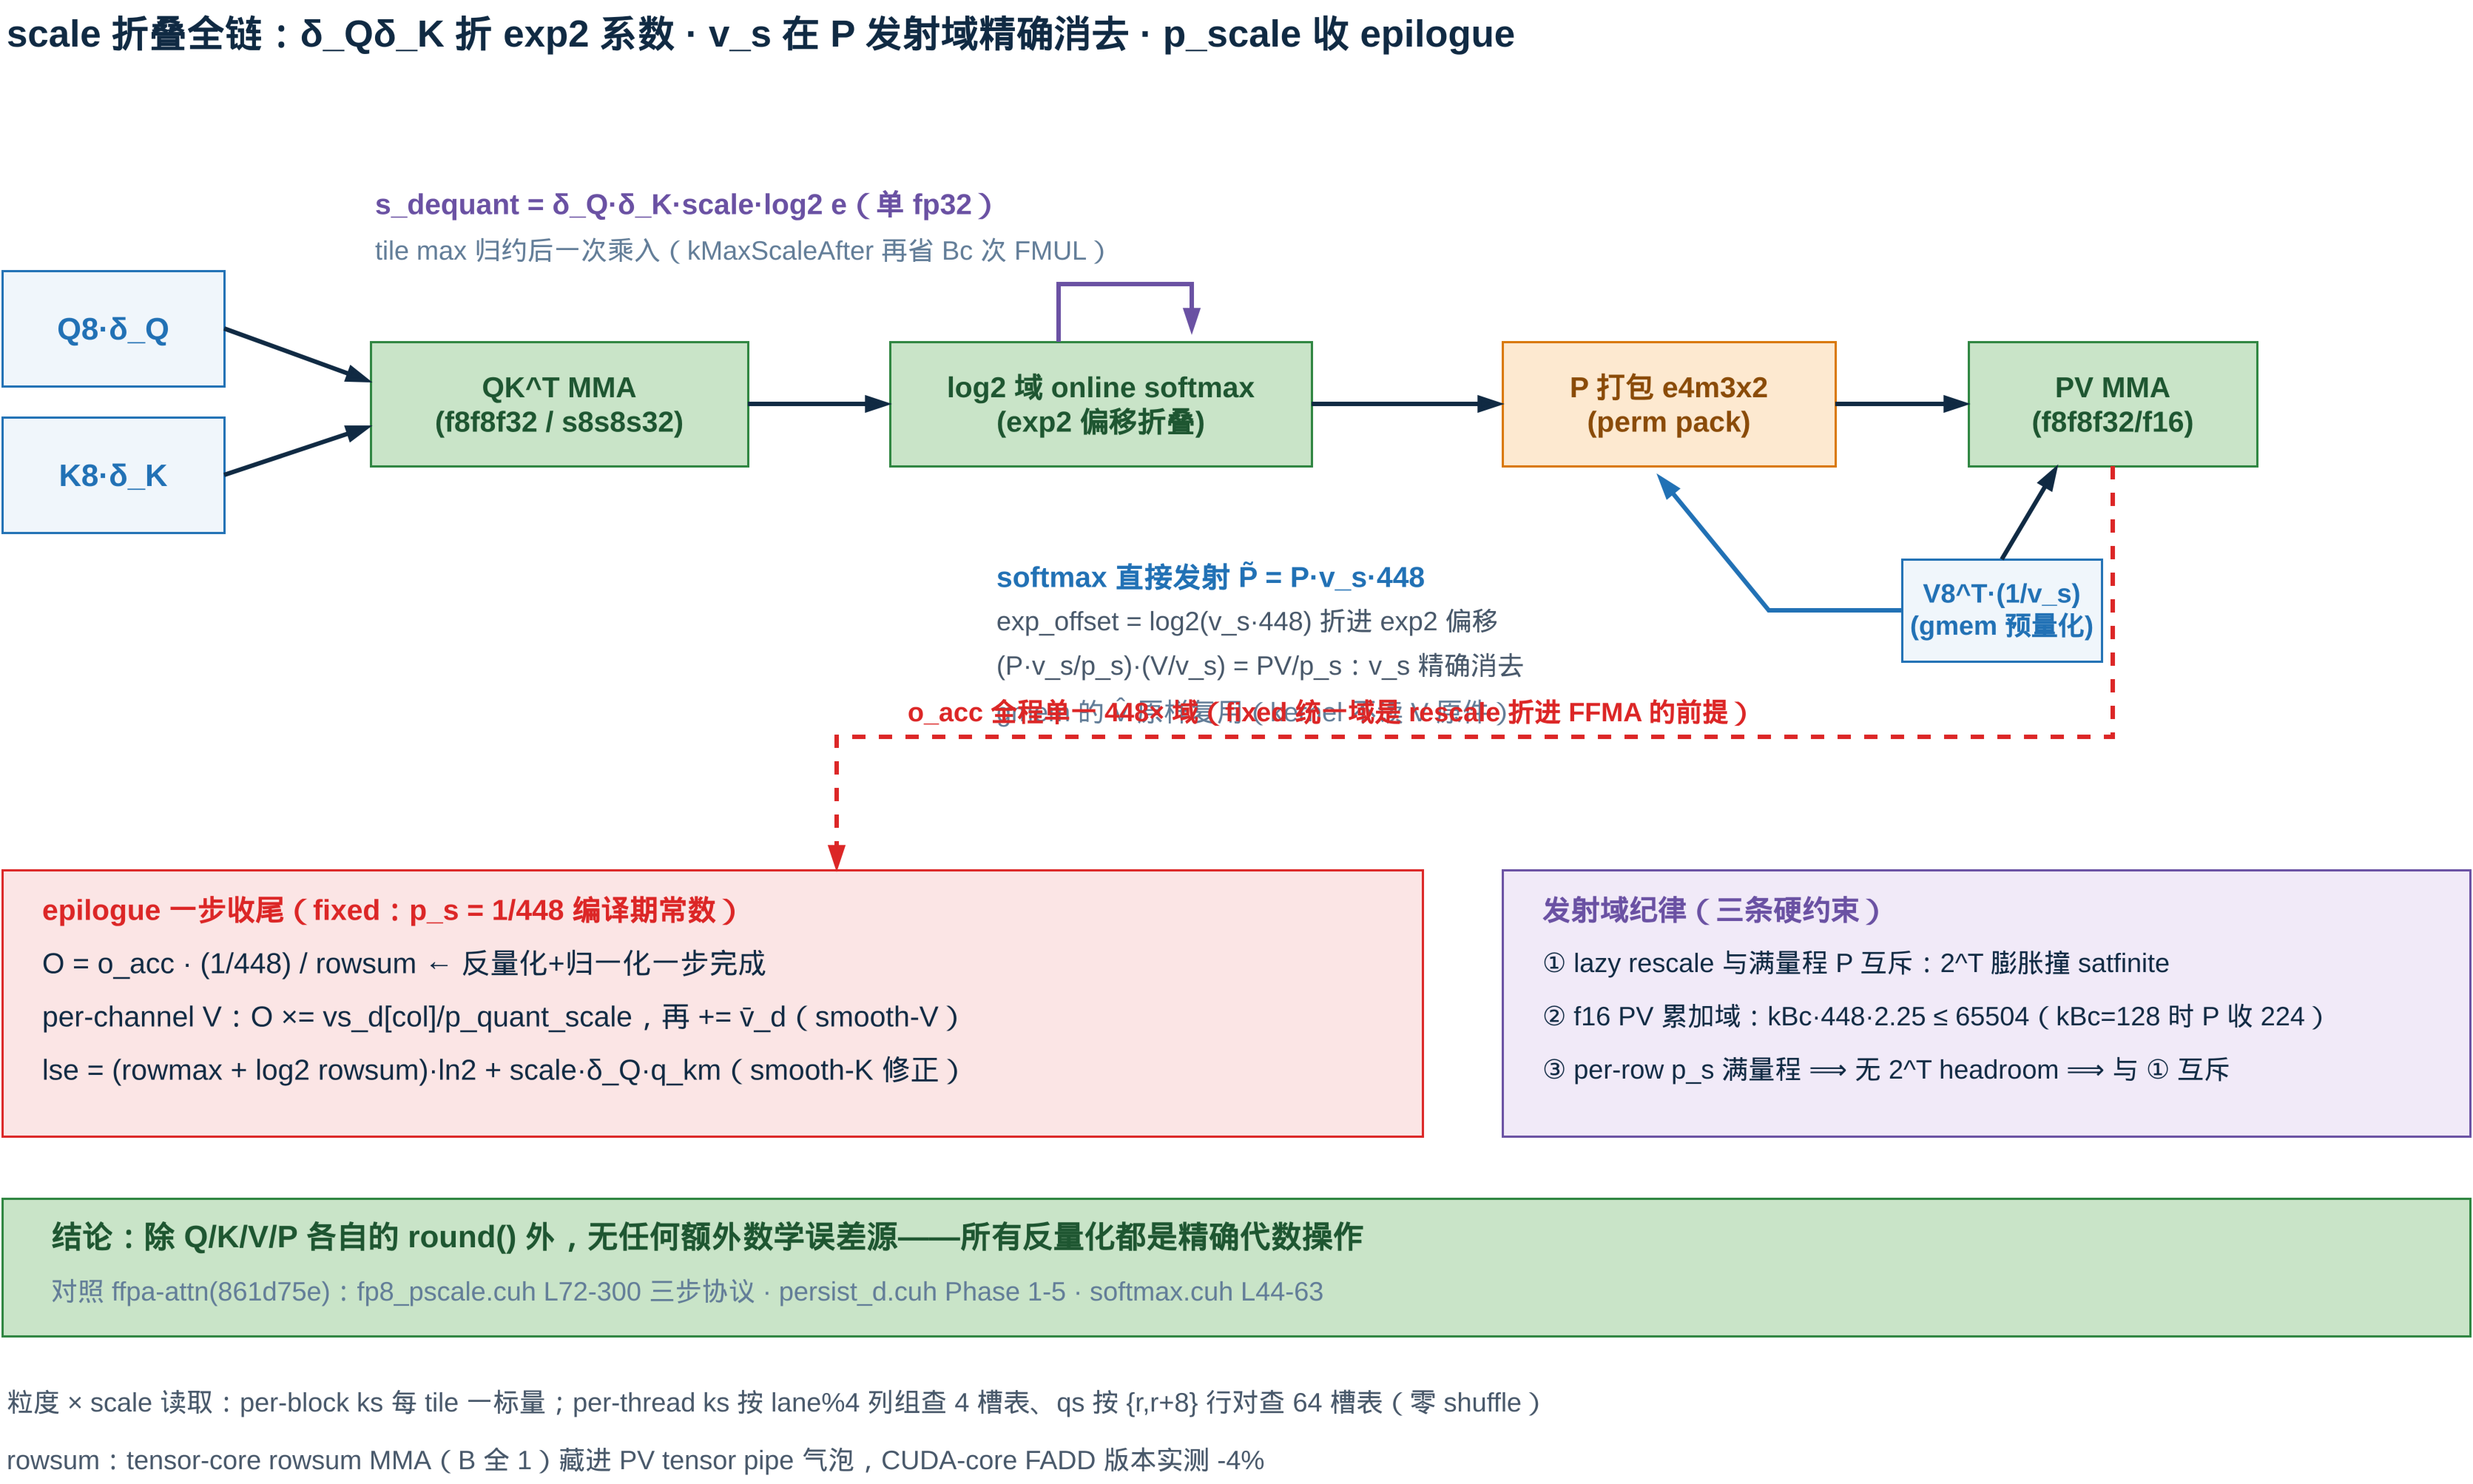
\includegraphics[width=0.98\textwidth]{figures/fig-29-1-scale-folding.png}
  \caption{scale 折叠全链数据流：$\delta_Q\delta_K$ 折进 exp2 系数、$v_s$
  在 P 发射域消去、$p_{scale}$ 收在 epilogue——除 round() 外无额外误差源。}
  \label{fig:29-scale-folding}
\end{figure}

\begin{figure}[H]
  \centering
  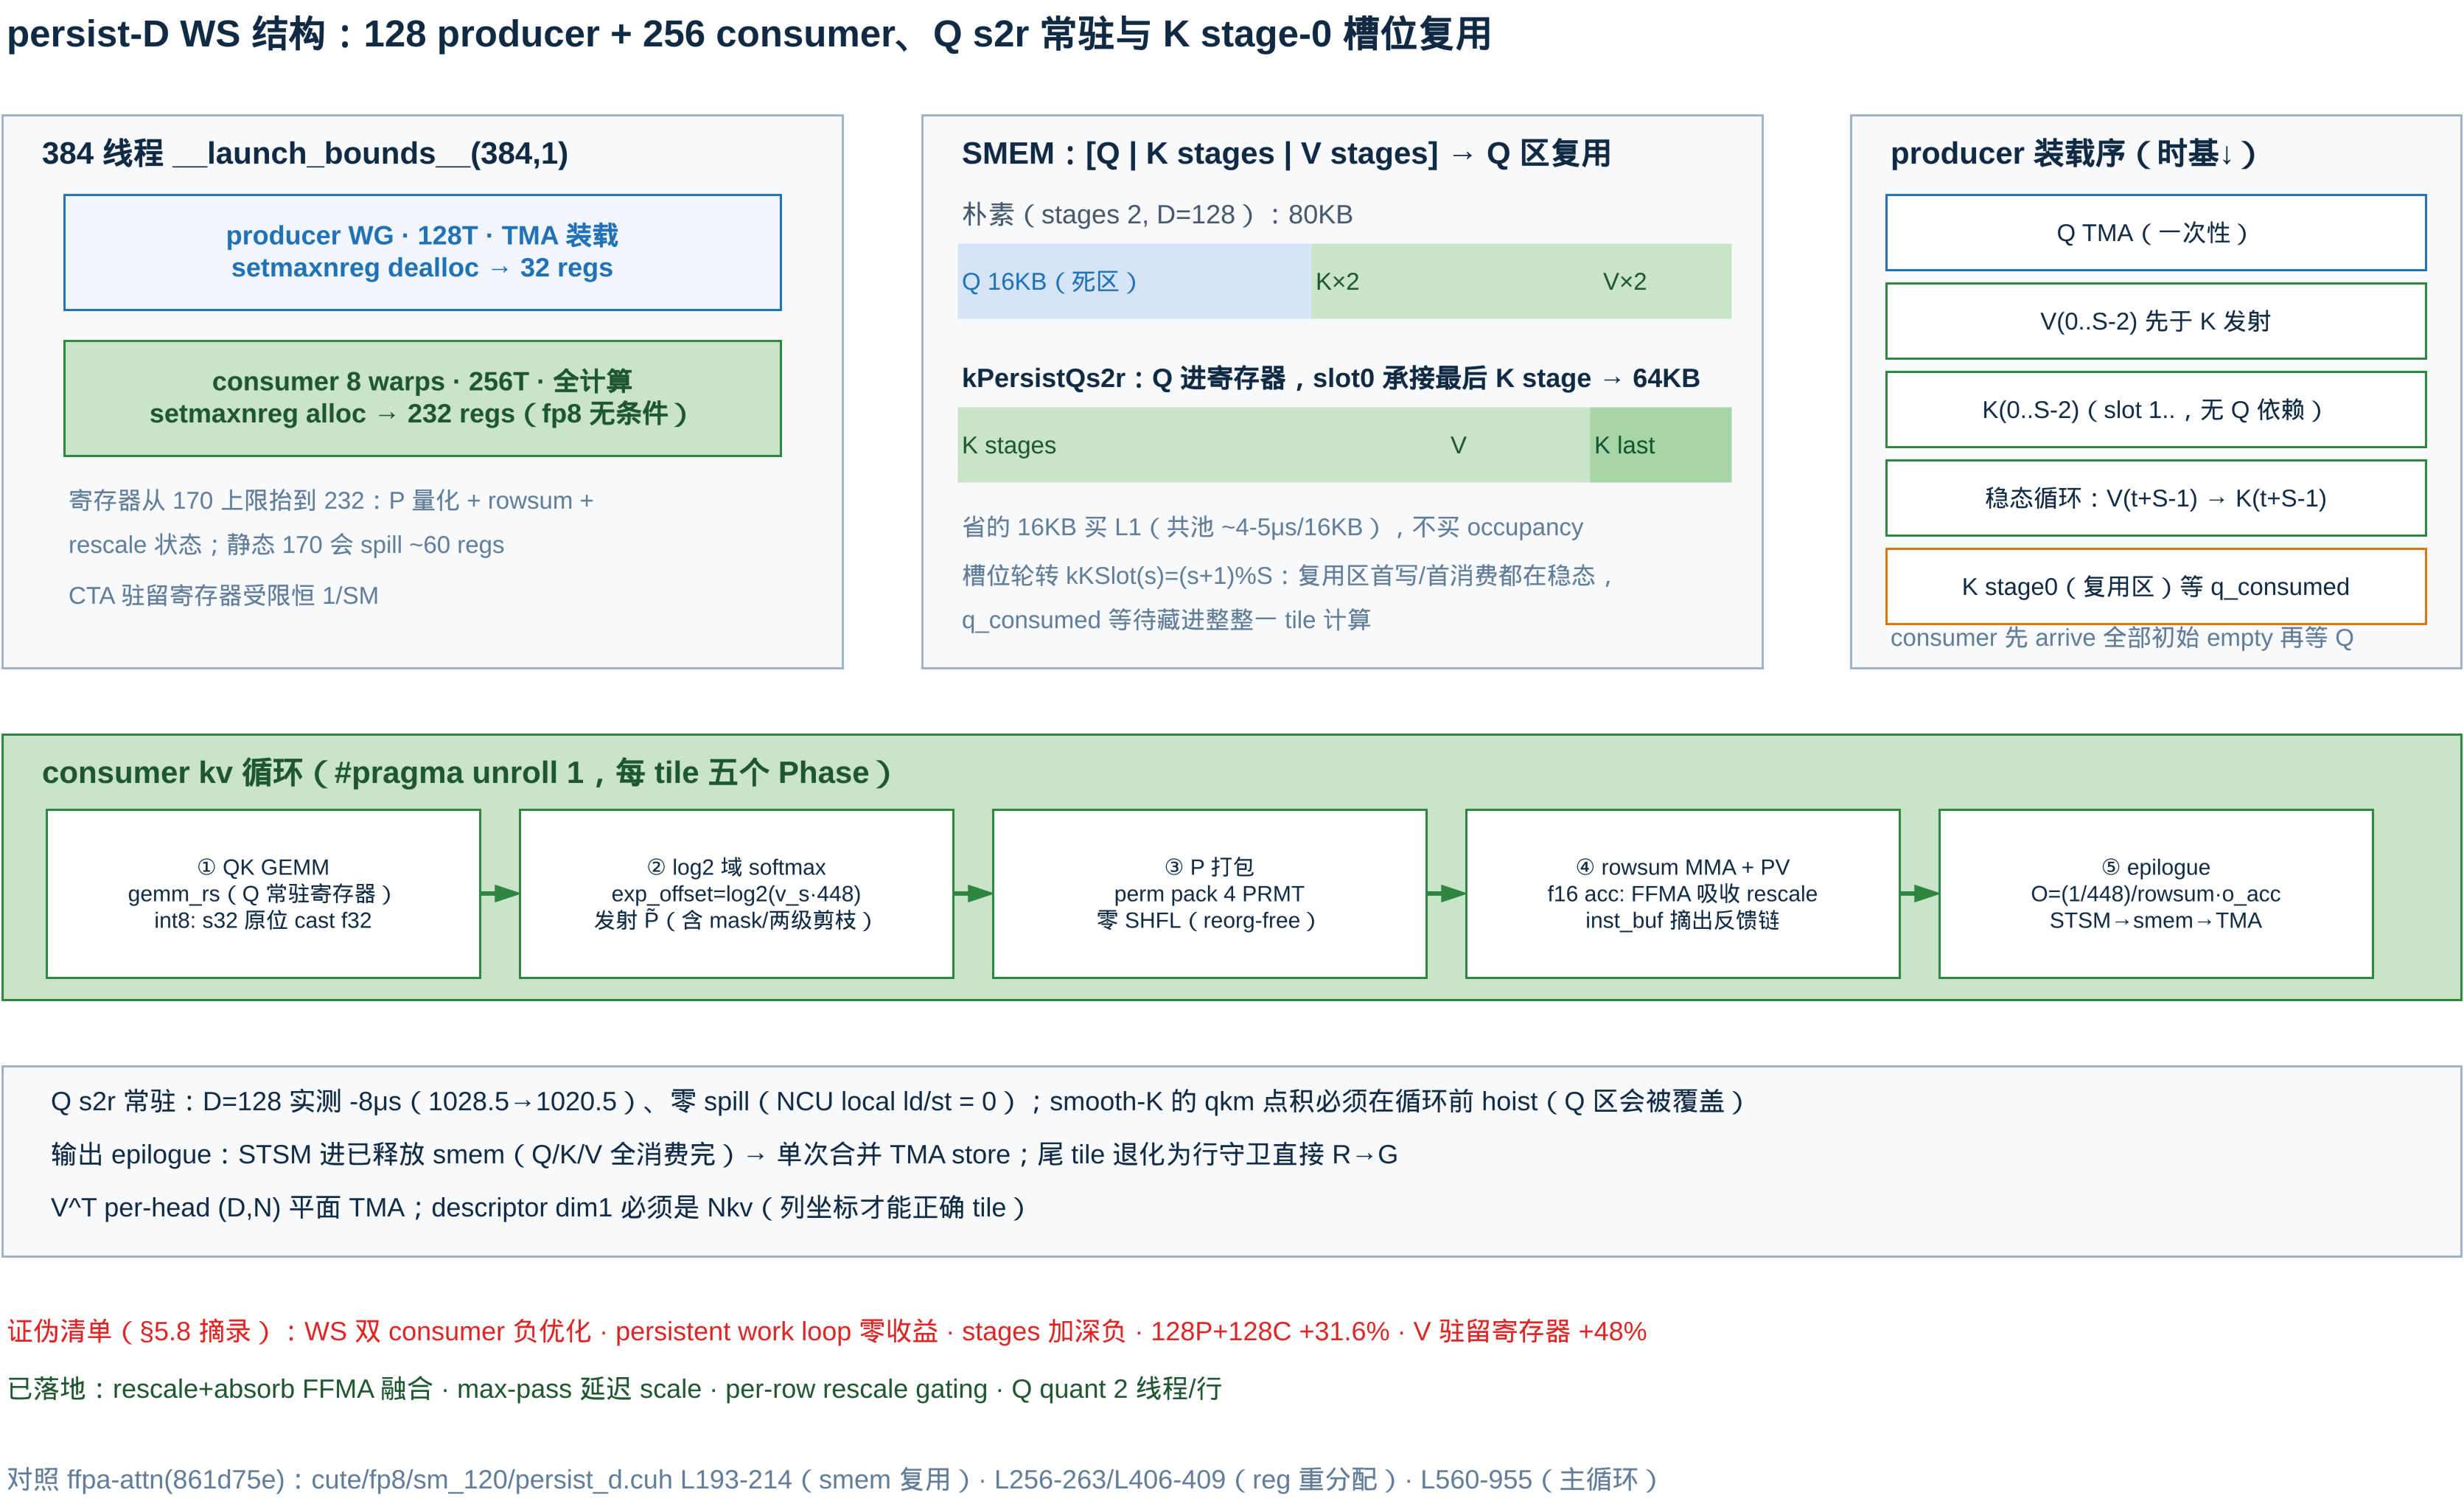
\includegraphics[width=0.98\textwidth]{figures/fig-29-2-persist-d-ws.png}
  \caption{persist-D WS 结构：128P+256C、setmaxnreg 32/232、Q s2r 常驻与
  K stage-0 槽位轮转的 smem 复用、STSM+TMA 输出。}
  \label{fig:29-persist-d-ws}
\end{figure}

\begin{figure}[H]
  \centering
  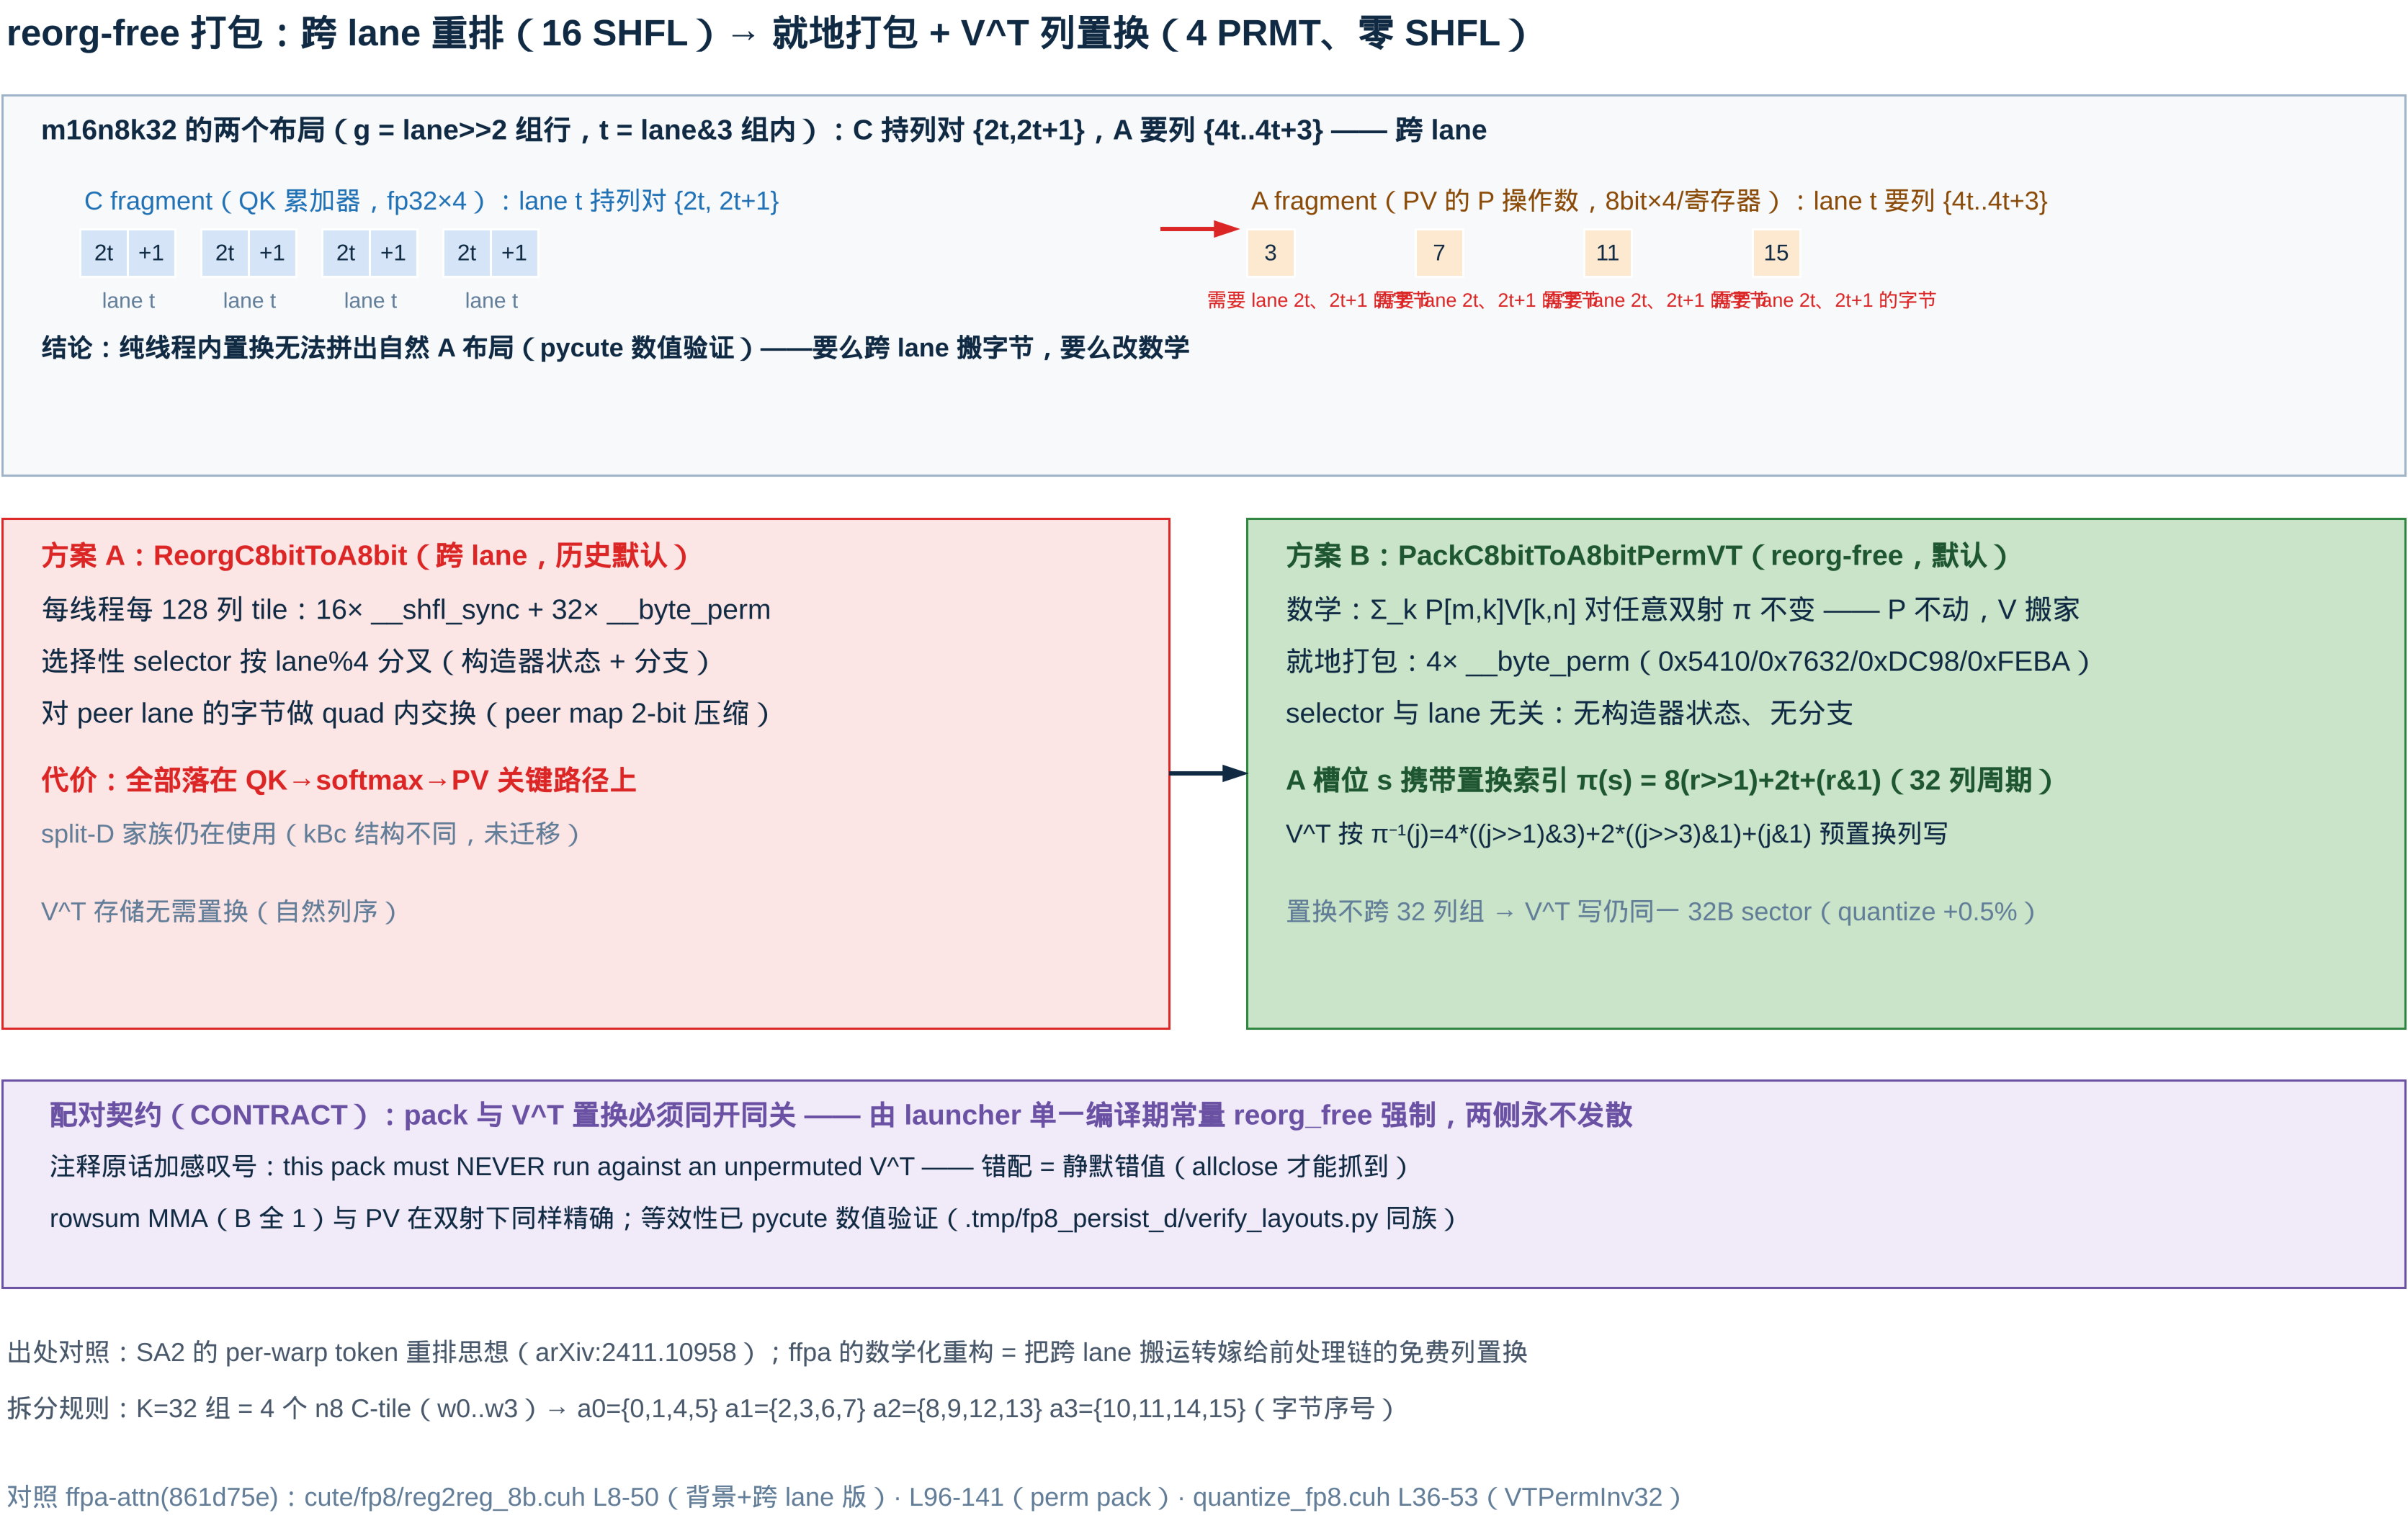
\includegraphics[width=0.98\textwidth]{figures/fig-29-3-reorg-free.png}
  \caption{reorg-free 打包对照：跨 lane 重排（16 SHFL）vs 就地打包 + $V^{\top}$
  列置换（4 PRMT、零 SHFL），归约轴双射不变性保证精确等价。}
  \label{fig:29-reorg-free}
\end{figure}

\section{性能分析}

\subsection{本机实测（RTX PRO 5000，B1 H32 N8192，bench 默认配置）}

\begin{center}
\begin{tabular}{llcccc}
\toprule
$D$ & task & FFPA & SDPA & TFLOPS & speedup \\
\midrule
64  & self-attn & 1.91ms & 2.40ms & 288T & 1.26$\times$ \\
64  & causal    & 1.16ms & 1.34ms & 237T & 1.16$\times$ \\
128 & self-attn & 3.02ms & 5.12ms & 365T & \textbf{1.70$\times$} \\
128 & causal    & 1.85ms & 2.68ms & 297T & 1.45$\times$ \\
192 & self-attn & 4.58ms & 7.27ms & 360T & 1.59$\times$$^{*}$ \\
\bottomrule
\end{tabular}
\end{center}
$^{*}$D=192 存在正确性 bug（29.7.1~节），速度数据仅供参考。D=64 的收益
小于 D=128 是因为 attention 的算术强度随 $D$ 下降、quantize aux 链占比
上升。kernel 级与 SageAttention 对比稳定 $+1.1\sim2.3\%$（仓库 NCU 记录）。

\subsection{微优化到顶：一份「证伪清单」的价值}

persist-D 的结构优化路线已被系统实测证伪（完整清单见仓库 RFC
\S5.8）：WS 双 consumer（FA3 式 2$\times$128T）负优化；persistent work
loop 零收益（tensor-bound 77\%）；stages 加深负（K2V2 预取已领先）；
v2/v3/v5（128P+128C、无 WS、V 驻留寄存器）分别 $+31.6\%$/追平/$+48\%$；
cluster 化无 DSMEM 需求、持平或更慢；CUDA-core row-sum 替代 tensor
rowsum MMA $-4\%$。\textbf{已落地的优化}（D=128）：rescale+absorb FFMA
融合、max-pass 延迟 scale、per-row rescale gating、Q quant 2 线程/行。
这份「负结果清单」与正结果同样重要——它把后续优化方向的搜索空间
压缩到了 engine 层（aux 链 overlap）。

\subsection{带宽与算术的边界}

D=128、N=8192 时主 kernel 365T FLOPS 对应的 DRAM 流量很小（$O(N\cdot D)$
量级 workspace 单遍），瓶颈在 tensor pipe 与 softmax 的依赖链——与
fp16 家族同构，但 fp8 的 MMA 吞吐翻倍使 softmax/P 打包的相对占比上升，
这也是 \texttt{kMaxScaleAfter}、FFMA 吸收融合这类\textbf{指令级}优化
在此路径收益显著的原因。

\section{实践经验}

\subsection{案例：D=192 正确性 bug 的定位（真实故事）}\label{sec:29-d192}

写本章的 bench 验证时发现 \texttt{--cuda-impl fp8 --D 192}
allclose 失败（fp16/bf16 双双 ❌），而 D=64/128 全绿。定位过程本身是
一份方法论示范：
\begin{enumerate}[itemsep=1pt,topsep=2pt]
  \item \textbf{误差量级分类}：max\_abs=2.66 vs mean\_abs=0.011——均值是
        正常 fp8 精度，最大值是灾难级 $\Rightarrow$ \textbf{正确性 bug}
        （个别行错），不是精度不足；
  \item \textbf{行模式定位}：per-row max 直方图显示坏行集中在
        $row\bmod128\in[64,127]$（每个 128 行 Q tile 的后半）；
  \item \textbf{N 缩放}：N=512 时几乎全错、N=8192 时只剩 11\% 行错
        ——错误随 N 稀释，说明错的是\textbf{特定 (row, kv-tile) 组合}而非
        系统性索引错位；
  \item \textbf{配置矩阵消去}：默认/纯 fp8 f32acc/int8+f16acc/no-smK/
        per-thread/per-channel 全部 ❌ $\Rightarrow$ 与量化 knob 无关，
        bug 在 D=192 特有的主 kernel 路径（$kBc{=}64$ 变体、SW64 swizzle、
        或 quantize 侧 kBlockRows 与 kBc 的一致性）；
  \item \textbf{fp16 对照}：fp16 CUTE 路径 D=192 完全正确
        （max=0.0001）$\Rightarrow$ 输入布局/TMA/寻址层无辜，责任圈定在
        fp8 专属代码。
\end{enumerate}
教训：\textbf{「速度好+均值好」不等于正确}——bench 的 allclose 是唯一
硬门槛；误差的 max/mean 分裂是「个别行错」的强信号；行号模 tile 尺寸的
直方图能直接把 bug 锚到 tile 结构的哪一半。

\subsection{考据：sm\_89 的 cp.async 变体}

同文件名在 \texttt{cute/fp8/sm\_89/persist\_d.cuh} 有一个 Ada 变体：
无 TMA/mbarrier，用 sm80 装载协议（cp.async + \texttt{wait<2S-1>}）复用
sm120 的计算层（int8 QK / fixed p\_scale / f8f8f16 PV），256T non-WS。
其 NCU 结论（依赖链/发射受限，\texttt{math\_pipe\_throttle} 1.32 $\gg$
\texttt{wait} 0.82）与深流水零收益的证伪记录，是「同一算法在不同装载
协议下瓶颈漂移」的绝佳对照。本节不展开，读者按需查阅源码头注释。

\section{常见坑}

\begin{enumerate}[itemsep=1pt,topsep=2pt]
  \item \textbf{P 是 online 量化，无法离线校准}：Q/K/V 都能离线 smoothing
        /per-channel 校准，P 每 tile 现算现量化，值域与分布逐行剧变
        （causal 早行近 one-hot、dense 行近均匀）——只能选固定/保守发射域。
        这是量化 attention 精度损失的主要根源之一（实测 P 0.11 与 QK 0.13
        同量级、V 0.19 最大）。
  \item \textbf{满量程 P 与 lazy rescale 互斥}：发射域铺满 448 后 stale max
        的 $2^T$ 膨胀必然 satfinite（29.3.3~节）；fp8 traits 直接关掉
        lazy rescale，且 f16 acc 路径把 rescale 融进吸收 FFMA 后延迟惩罚
        消失。
  \item \textbf{kVTPerm 配对是编译期纪律}：\texttt{PackC8bitToA8bitPermVT}
        对未置换的 $V^{\top}$ 运行 = 静默错值。配对由 launcher 单一常量
        强制；绕过 launcher 直接调 kernel 没有保护。
  \item \textbf{f16 PV 累加域}：$kBc\cdot448\cdot2.25\le65504$ 的编译期
        检查不过时 P 域自动收到 224——不理解这条约束会以为 P 域「有时
        448 有时 224」是随机行为。
  \item \textbf{early rows 的 ESS 幅度放大}（27.3.8~节）：causal 前几行
        ESS$\approx$1、幅度 $3.1\sigma$，fp8 每级 $\sim$5\% 相对误差换算
        成 15$\times$ 于 dense 的绝对误差；「早行 fp16 QK」不解决问题
        （V 量化是最大单项），hybrid 全链 fp16 才有效。
  \item \textbf{D=192（$kBc{=}64$ 变体）当前有正确性 bug}：29.7.1~节的
        定位记录；在修复前避免在生产使用该 headdim 的 fp8 persist-D。
\end{enumerate}

\section{面试要点速查}

\begin{enumerate}[itemsep=1pt,topsep=2pt]
  \item fp8 attention 的所有 scale 是如何消去的？
        （$\delta_Q\delta_K$ 折 exp2 系数；$v_s$ 折 P 发射域精确消去；
        $p_{scale}$ 收 epilogue——式~\ref{eq:29-sdequant}--\ref{eq:29-threestep}。）
  \item 为什么 P 的量化只能 fixed/保守，不能离线校准？
        （P 每 tile 现算、分布逐行剧变；离线对象必须前向开始前存在。）
  \item lazy rescale 与满量程 P 为什么互斥？（$2^T$ 膨胀 vs 448 satfinite，
        29.3.3~节；f16 acc 路径 FFMA 吸收让 rescale 免费。）
  \item f16 PV 累加器的域怎么算？（$\pm65504/32=2047$；P 448 $\times$ V
        2.25 $=1008$ ✓——SA2++ 双侧收窄 vs ffpa 单侧压 V 的差异。）
  \item reorg-free 打包省了什么、代价是什么？（16 SHFL+32 PRMT $\to$
        4 PRMT 零 SHFL；代价 $V^{\top}$ 列置换预写 + 编译期配对纪律，
        式~\ref{eq:29-perm-inv}。）
  \item Q 的 s2r 常驻为什么省钱？省的是 occupancy 吗？
        （不是——省 smem（16KB Q 区复用）$\to$ 买 L1 共池容量，
        $\sim$4--5$\mu s$/16KB；CTA 驻留本就寄存器受限。）
  \item fp8 persist-D 的 D 范围与家族分工？（$\le$224 %32；更大走
        split-D M8N1 / M4N2，第~\ref{ch:30}~章。）
\end{enumerate}

\section{最小测试与动手实验}

\begin{lstlisting}[style=console]
# 环境（Card 7，小 headdim 放行）
$ conda activate cdit
$ export CUDA_VISIBLE_DEVICES=7 FFPA_CUDA_ALLOW_SMALL_D=1

# [A] persist-D 域内全绿组合：D=64 / 128
$ python -m ffpa_attn.bench --fwd-backend cuda --cuda-impl fp8 \
    --tasks self-attn,causal --D 128 --no-bwd --show-allclose
# self-attn fp16  8192/8192  3.02ms  365T  1.70x  allclose ✅
# causal    fp16  8192/8192  1.85ms  297T  1.45x  allclose ✅

# [B] 配置显式声明（int8 QK + f16 PV acc）
$ python -m ffpa_attn.bench --fwd-backend cuda --cuda-impl fp8 \
    --tasks self-attn --D 128 --no-bwd --show-allclose \
    --fp8-qk-mm-type int8 --fp8-pv-acc-type f16
# 3.08ms  357T  1.67x  allclose ✅

# [C] D=192：正确性 bug 复现（29.7.1 节）
$ python -m ffpa_attn.bench --fwd-backend cuda --cuda-impl fp8 \
    --tasks self-attn --D 192 --no-bwd --show-allclose
# allclose ❌  ← 坏行集中在 row%128 ∈ [64,127]
\end{lstlisting}

\textbf{实验 1（scale 流向追踪）}：把 \texttt{persist\_d.cuh} 的
Phase 1--5 各自在纸上标出「哪个 scale 在哪条指令上被乘/消去」，对照
图~\ref{fig:29-scale-folding}——练到能默写三步协议。
\textbf{实验 2（发射域 A/B）}：\texttt{FFPA\_FP8\_PQUANT\_PER\_ROW=1}
重跑 [A]，观察精度提升与速度代价（per-row 归约 + $o\_tile$ 暂存）。
\textbf{实验 3（bug 定位复演）}：按 29.7.1~节步骤用 PyTorch 复现 D=192
的行模式直方图（脚本思路：per-row max diff $>$ 0.1 统计
$row\bmod128$）——把「速度好+均值好 $\neq$ 正确」变成肌肉记忆。
\textbf{实验 4（lazy rescale 证伪）}：读 \texttt{attn\_traits.cuh}
L31--37 注释，回答「为什么 fp8 关掉 lazy rescale 而 fp16 开着」。

\section*{延伸阅读}
\begin{itemize}[itemsep=0pt,topsep=2pt]
  \item SageAttention2（arXiv:2411.10958）：per-warp token 重排与 int8 QK
        的原始出处（reorg-free 打包的对照原型）。
  \item SageAttention2++（arXiv:2505.21136）\S3.1：f16 PV 累加域约束
        （$P_r\times V_r\le2047$）的推导。
  \item FlashAttention-4（arXiv:2603.05451）：lazy rescale 与量化域交互
        （本章 29.3.3~节的反例来源）。
  \item ffpa-attn \texttt{reg2reg\_8b.cuh} 头注释：C$\to$A fragment
        布局的 PTX 级推导与 pycute 数值验证记录。
  \item ffpa-attn 仓库 RFC \S5.8：persist-D 结构优化的完整证伪清单
        （负结果的科学价值）。
\end{itemize}

% ch30-fp8-split-d-m4n2.tex — FP8(三)：split-D 与 M4N2——大 D 的两堵墙（RFC-K4）
% 源码：ffpa-attn(861d75e) cute/fp8/sm_120/split_d.cuh(956L) + split_d_m4n2.cuh(989L)
%       + attn_traits.cuh(L109-311) + softmax.cuh(L74-231) + dispatch/cute_fp8.cuh
\chapter{FP8（三）：split-D 与 M4N2——大 $D$ 的两堵墙}\label{ch:30}

\section{本章导读}

第~\ref{ch:29}~章的 persist-D 把整个 $K$ tile（$B_c\times D$）一次装进
smem、让单个 warp 独占 $O$ 的全部 $D$ 列。这在 $D\le 224$ 时是最优解；
但 $D$ 继续增大，会同时撞上\textbf{两堵墙}：

\begin{enumerate}[itemsep=0pt,topsep=2pt]
  \item \textbf{smem 墙}：$K$ tile 字节数 $O(D)$，99KB 预算装不下——
        由 \textbf{split-D}（D 维分块）解决；
  \item \textbf{寄存器墙}：$O$ 累加器 $O(D)$ 个 f32 寄存器/线程，逼近
        255 上限——由 \textbf{M4N2 TiledMMA}（atom 布局重排）解决。
\end{enumerate}

两堵墙正交：只做 split-D，寄存器照旧 $O(D)$；只做 M4N2，smem 照旧装不下。
ffpa-attn 的 dispatch 按 $D$ 三分（\texttt{dispatch/\allowbreak{}cute\_fp8.cuh}
L60--64）：

\begin{center}
\begin{tabular}{@{}llll@{}}
\toprule
$D$ 范围 & kernel & atom 布局 & $O$ 寄存器/线程 \\
\midrule
$D\le 224$ & \texttt{persist\_d}（第~\ref{ch:29}~章） & M8N1 & $D/2$ \\
$224<D<768$ & \texttt{split\_d.cuh}（本章） & M8N1 & $D/2$ \\
$D\ge 768$ & \texttt{split\_d\_m4n2.cuh}（本章） & M4N2 & $D/4$ \\
\bottomrule
\end{tabular}
\end{center}

本章先推导 split-D 的分块恒等式（为什么它是\textbf{精确}变换，一个比特
都不差），再建立 M4N2 的寄存器压力模型（为什么 $N$ 维劈开是数学上的唯一
出口），最后走读两个 kernel 的实现差异——特别是 M4N2 带来的多笔新代价：
P 的 SMEM roundtrip、跨 N-warp softmax 归约、$k_{Br}$ 减半与量化块
错位等。所有机制均以
fp8 家族为主线；fp16 家族同构（第~\ref{ch:25}~章已见其 fp16 版），fp4
家族见第~\ref{ch:32}~章。

\section{问题与动机}

\subsection{两堵墙的数量级}

smem 墙好算：fp8 下 1B/元素，$B_c=128$ 的 $K$ tile 在 $D=512$ 时是
64KB，加上 V stage 与 Q 就超 99KB 预算。persist-D 靠「K 槽位 0（Q 区）
复用给最后一个 K stage」
挤过去的前提是 $D\le 224$；$D$ 再大，唯一的路是把 $D$ 切块流水。

寄存器墙隐蔽一些。m16n8k32 atom 的 C-fragment 每 thread 持 4 个 f32；
M8N1 布局（8 个 M-warp、N 维单 warp 满编）下单 warp 独占输出的完整 $D$
列，$k_{Br}=128$ 时 $O$ 累加器寄存器数是
\begin{equation}\label{eq:30-oacc-m8n1}
O_{\text{acc}}=\frac{k_{Br}\cdot D}{256\ \text{threads}}=\frac{D}{2}
\quad(\text{f32 regs/thread},\ k_{Br}=128),
\end{equation}
$D=512$ 时 256 个寄存器\textbf{超出上限 1 个}（255）——边缘 spill；$D\ge 896$ 大量
spill 直接崩塌。实测（5090，fp16 家族同构）：$D=1024$ 时 M8N1 的
$O_{\text{acc}}=512$ regs 溢出到 local memory，吞吐掉到 $\sim$100T；
而 M4N2 同 $D$ 边缘 spill 仍有 154T。

\subsection{split-D 与 M4N2 各管一堵墙}

\textbf{split-D} 回答「smem 怎么装下」：把 $D$ 切成 $D/k_{VDChunk}$ 个
chunk，K/V 的 TMA 与 MMA 都按 chunk 流水，smem 只需常驻
$(k_{Br}+k_{Bc})\times k_{QKDChunk}+k_{Bc}\times k_{VDChunk}$ 每 stage，
与总 $D$ 无关。\textbf{M4N2} 回答「寄存器怎么装下」：把 atom 布局从
$(8,1,1)$ 换成 $(4,2,1)$——4 个 M-warp \textbf{乘} 2 个 N-warp——让每
thread 的 $O$ 列持有量减半（\ref{sec:30-regmodel}~节的推导）。

代价各自独立：split-D 多了每 chunk 一次 producer-consumer 握手；M4N2
使 $k_{Br}$ 从 128 减到 64（CTA 数翻倍）、P 必须走 SMEM roundtrip、
softmax 需要跨 N-warp 归约。交叉点在 $D=768$：之下 M8N1 更快（无
roundtrip 开销、$k_{Br}$ 大一倍），之上 M4N2 的寄存器红利开始统治
（30.6.2~节）。

\subsection{causal 精度的已知边界}

\texttt{split\_d.cuh} 的头注释（L40--43）声明了 causal 精度边界：
逐元素误差上界——causal 早期行 attend 的 key 少，
QK/P 量化误差无法被平均——
$O$ 误差可保持在 $10^{-1}$ 量级但 lse 误差可达 $\sim 6\times10^{-2}$
（近 1 概率的 e4m3 舍入），dense 则 $\sim 4\times10^{-3}$（m4n2 头注释无同款
声明，但精度结构相同）。本机实测
（30.6~节）三个 $D$ 的 causal 误差模式完全一致：序列前
$\sim$30\% 的行误差大、其余干净、dense 全绿——这是 fp8 路径的
\textbf{已知特性}而非 bug，工程解法是 hybrid（前若干行走 fp16
stage-1，\texttt{dispatch/cute\_fp8.cuh} L55--58 的 FC-3 注释），
不在本章展开。

\section{数学原理}

\subsection{split-D 分块恒等式：精确，不是近似}\label{sec:30-identity}

设 $D=\mathcal{D}_0\cup\mathcal{D}_1\cup\cdots$ 按 chunk 划分。QK 侧
$D$ 是\textbf{归约维}：
\begin{equation}\label{eq:30-qk-split}
S=QK^{\top}=\sum_{c}Q_{:,\mathcal{D}_c}\,K^{\top}_{:,\mathcal{D}_c},
\end{equation}
每个 chunk 一次 MMA \textbf{累加进同一个} $S$ fragment。fp8 路径 f32
累加；int8 路径 s32 累加（精确，$\ll 2^{31}$）后一次性 cast（L495--503）
——split 不引入任何新的舍入点。PV 侧 $D$ 是\textbf{输出列维}：
\begin{equation}\label{eq:30-pv-split}
O_{:,\mathcal{D}_c}=P\,V^{\top}_{\mathcal{D}_c,:},
\end{equation}
各 chunk 的 $O$ 段\textbf{独立累加}，互不干扰。

关键观察：softmax 的行统计（$m_r$、$\ell_r$）是\textbf{KV 行维的量}，
与 $D$ 的切分完全无关——split-D \textbf{不产生}「每 chunk 各自的
row max/row sum」，所有 chunk 共享同一组 $(m,\ell)$，rescale 因子天然
一致。这就是 \texttt{split\_d.cuh} 的结构（L440--443 注释）：QK chunk
循环在 softmax \textbf{之前}全部完成（L446--483），softmax 之后 V
chunk 循环各自把 $P V^{\top}_{\mathcal{D}_c}$ 加进
\texttt{o\_acc\_storage[c]}（L678--756）。

\begin{figure}[H]
\centering
\begin{tikzpicture}[font=\scriptsize, >=Stealth]
  \node[anchor=south, font=\scriptsize\bfseries] at (6.6,0.62)
    {split-D 分块恒等式：QK 归约维累加，PV 输出列维独立};
  \node[anchor=south, font=\tiny] at (6.6,0.38)
    {示例 $D{=}128$（$k_{VDChunk}{=}64\Rightarrow 2$ 个 chunk；通用 $D/k_{VDChunk}$ 个）};
  \draw[fill=gray!18] (0,-0.75) rectangle (1.5,-0.15);
  \draw[fill=gray!55] (0,-1.55) rectangle (1.5,-0.95);
  \draw[thick] (0,-0.75) rectangle (1.5,-0.15);
  \draw[thick] (0,-1.55) rectangle (1.5,-0.95);
  \node at (0.75,-0.45) {$Q_{:,\mathcal{D}_0}$};
  \node at (0.75,-1.25) {$Q_{:,\mathcal{D}_1}$};
  \node[anchor=east, font=\tiny] at (-0.12,-0.45) {$Q$};
  \node[anchor=east, font=\tiny] at (-0.12,-1.25) {（$M{\times}D$）};
  \draw[fill=gray!18] (0,-2.45) rectangle (1.5,-1.85);
  \draw[fill=gray!55] (0,-3.25) rectangle (1.5,-2.65);
  \draw[thick] (0,-2.45) rectangle (1.5,-1.85);
  \draw[thick] (0,-3.25) rectangle (1.5,-2.65);
  \node at (0.75,-2.15) {$K^{\top}_{\mathcal{D}_0,:}$};
  \node at (0.75,-3.0) {$K^{\top}_{\mathcal{D}_1,:}$};
  \node[anchor=east, font=\tiny] at (-0.12,-2.15) {$K^{\top}$};
  \node[anchor=east, font=\tiny] at (-0.12,-3.0) {（$D{\times}B_c$）};
  \draw[->] (1.55,-0.45) -- (2.42,-0.82);
  \draw[->] (1.55,-2.15) -- (2.42,-1.08);
  \draw[->] (1.55,-1.25) -- (2.42,-2.38);
  \draw[->] (1.55,-3.0) -- (2.42,-2.62);
  \draw[thick] (2.5,-0.95) circle (0.40);
  \node at (2.5,-0.95) {\tiny MMA};
  \draw[thick] (2.5,-2.55) circle (0.40);
  \node at (2.5,-2.55) {\tiny MMA};
  \draw[->] (2.9,-1.15) -- (3.28,-1.48);
  \draw[->] (2.9,-2.35) -- (3.28,-2.02);
  \draw[thick] (3.62,-1.75) circle (0.34);
  \node at (3.62,-1.75) {$\Sigma_c$};
  \draw[->] (3.96,-1.75) -- (4.45,-1.75);
  \draw[fill=white, thick] (4.5,-2.4) rectangle (6.0,-1.1);
  \node at (5.25,-1.62) {$S$ fragment};
  \node at (5.25,-2.12) {\tiny 同一 C 累加器};
  \node[anchor=south, font=\tiny, align=center] at (5.25,-1.02)
    {归约维：chunk 累加\\（式~\ref{eq:30-qk-split}，无新舍入点）};
  \draw[->] (6.05,-1.75) -- (6.55,-1.75);
  \node[above, font=\tiny] at (6.3,-1.68) {$P$};
  \draw[fill=white, thick] (6.6,-2.3) rectangle (8.0,-1.2);
  \node at (7.3,-1.62) {softmax};
  \node at (7.3,-2.10) {\tiny 全 $D$ 一次};
  \draw[->] (8.05,-1.6) -- (8.55,-1.08);
  \draw[->] (8.05,-1.9) -- (8.55,-2.42);
  \draw[thick] (8.95,-0.95) circle (0.40);
  \node at (8.95,-0.95) {\tiny MMA};
  \draw[thick] (8.95,-2.55) circle (0.40);
  \node at (8.95,-2.55) {\tiny MMA};
  \draw[fill=gray!18] (10.3,-0.85) rectangle (11.8,-0.25);
  \draw[fill=gray!55] (10.3,-3.5) rectangle (11.8,-2.9);
  \draw[thick] (10.3,-0.85) rectangle (11.8,-0.25);
  \draw[thick] (10.3,-3.5) rectangle (11.8,-2.9);
  \node at (11.05,-0.55) {$V^{\top}_{\mathcal{D}_0,:}$};
  \node at (11.05,-3.2) {$V^{\top}_{\mathcal{D}_1,:}$};
  \node[anchor=west, font=\tiny] at (11.92,-0.55) {$V^{\top}$};
  \node[anchor=west, font=\tiny] at (11.92,-3.2) {（$D{\times}B_c$）};
  \draw[->] (10.25,-0.55) -- (9.38,-0.9);
  \draw[->] (10.25,-3.2) -- (9.38,-2.6);
  \draw[fill=white, thick] (12.5,-1.25) rectangle (13.9,-0.65);
  \node at (13.2,-0.95) {$O_{:,\mathcal{D}_0}$};
  \draw[fill=white, thick] (12.5,-3.1) rectangle (13.9,-2.5);
  \node at (13.2,-2.8) {$O_{:,\mathcal{D}_1}$};
  \draw[->] (9.35,-0.95) -- (12.45,-1.05);
  \draw[->] (9.35,-2.55) -- (12.45,-2.7);
  \node[anchor=north, font=\tiny, align=center] at (13.2,-3.15)
    {$O=[\,O_{:,\mathcal{D}_0}\mid O_{:,\mathcal{D}_1}\,]$：输出列维\\各 chunk 独立累加（式~\ref{eq:30-pv-split}）};
  \draw[fill=white, thick] (1.8,-4.95) rectangle (12.6,-4.45);
  \node[align=center] at (7.2,-4.7)
    {行统计 $(m_r,\ell_r)$：\textbf{KV 行维的量}——与 $D$ 切分完全无关，所有 chunk
     共享同一组（不产生 per-chunk 统计），rescale 因子天然一致};
  \draw[densely dashed] (7.3,-2.3) -- (7.3,-4.45);
  \draw[densely dashed] (8.95,-1.35) -- (8.95,-4.45);
  \draw[densely dashed] (8.95,-2.95) -- (8.95,-4.45);
\end{tikzpicture}
\caption{split-D 分块恒等式的数据流（30.3.1~节）。QK 侧：$D$ 是\textbf{归约维}，
各 chunk 的 $Q_{:,\mathcal{D}_c}K^{\top}_{\mathcal{D}_c,:}$ 累加进\textbf{同一个} $S$
fragment（式~\ref{eq:30-qk-split}，f32/s32 累加，不引入新舍入点）；PV 侧：$D$ 是
\textbf{输出列维}，各 chunk 独立累加出 $O_{:,\mathcal{D}_c}$ 列段
（式~\ref{eq:30-pv-split}），无任何合并。softmax 的行统计 $(m_r,\ell_r)$ 是 KV 行维
的量——与 $D$ 切分完全无关，所有 chunk 共享同一组（灰度 = chunk 身份，两图同语义）。}
\label{fig:30-split-identity}
\end{figure}

需要真正「合并行统计」的不是 split-D，而是 M4N2 的 N-warp 劈分
（\ref{sec:30-m4n2softmax}~节）。

\subsection{M4N2 的 N-warp 劈分与 softmax 合并协议}\label{sec:30-m4n2softmax}

M4N2 把 $B_c$（以及每个 $V$ chunk 的 $D$ 列）劈给 2 个 N-warp。于是
每行 softmax 的统计量只持有一半：
\begin{align}
m_r &= \max\bigl(m_r^{(C_0)},\ m_r^{(C_1)}\bigr),\label{eq:30-maxmerge}\\
\ell_r &= \ell_r^{(C_0)}+\ell_r^{(C_1)},\label{eq:30-summerge}
\end{align}
max 是 bitwise 与顺序无关的；sum 只有 fp32 舍入级差异。但两个 N-warp
交换后\textbf{必须持有相同的} $(m_r,\ell_r)$，否则后续 rescale 因子
不一致、$O$ 列段错位。

实现（\texttt{softmax.cuh} L74--231）用一块 1KB 的
\texttt{smem\_exchange}：布局 $[8\ \text{warps}][16\ \text{rows}]$ 两段
（max 段、sum 段），peer warp 是 $\texttt{warp\_id}\oplus 4$（翻转
N-warp 位）。协议刻意\textbf{只留一个 barrier}：

\begin{enumerate}[itemsep=0pt,topsep=2pt]
  \item 各 warp 算本 warp 的 tile max（warp 内 \texttt{shfl\_xor} 1/2
        归约），写 max 段，\texttt{\_\_syncthreads()}（L103--110）；
  \item 读自己与 peer 的 max 取全局，更新 $m$ 与 rescale 因子，
        发射 $P=\exp2(s\cdot\gamma-(m-\text{offset}))$，本 warp 的
        tile sum 写 sum 段——\textbf{不再 barrier}（L112--141）；
  \item 调用方紧接着的 P 写读 roundtrip 自带
        \texttt{\_\_syncthreads()}，顺带发布 sum 写；
        \texttt{finalize\_row\_sum\_m4n2}（L147--163）在 barrier 之后
        读两 warp 的 sum 相加，折进全局 $\ell_r$（L700--704）。
\end{enumerate}

省掉的是 3-sync 版本里专门的 sum 交换 barrier（每 KV tile 净省一次
CTA sync，sum 的发布搭 P roundtrip 便车）；代价是 max 段与 sum 段
\textbf{必须分开}，否则快 warp 可能在 peer 读走 max 之前用 sum 覆写它
（L92--95 的 RAW 注释）。fp8 变体 \texttt{online\_softmax\_fp8\_fixed\_m4n2}
（L174--239）在此基础上把第~\ref{ch:29}~章的
$\text{offset}=\log_2(v_s\cdot448)$ 折进 $\exp2$，tile sum 乘
$1/(v_s\cdot448)$ 后再写 sum 段，\texttt{finalize} 之后 $\ell_r$ 直接
落在真概率域。

lse 只由 \texttt{n\_warp==0} 写（两个 N-warp 共享同一批 Q 行，
\texttt{split\_d\_m4n2.cuh} L970）。

\subsection{寄存器压力模型：为什么只有减 $M_w$ 有效}\label{sec:30-regmodel}

m16n8k32 atom 每 warp 产 $[16,8]$ 的 C-fragment，每 thread 4 个 f32。
atom 布局 $(M_w,N_w,1)$ 下每 warp 沿 M 拿 $k_{Br}/(16M_w)$ 个 atom 行
片、沿 N 拿 $D/(8N_w)$ 列（跨 V chunk 累计），逐 thread 的 $O$
寄存器数是
\begin{equation}\label{eq:30-regthread}
O_{\text{acc}}
=4\cdot\frac{k_{Br}}{16M_w}\cdot\frac{D}{8N_w}
=\frac{D}{2N_w}\quad(\text{f32 regs/thread}),
\end{equation}
（M8N1/M4N2 都满足 $k_{Br}=16M_w$，即每 warp 恰好一片 M 方向 atom，
第一个因子为 1。）M8N1 给 $D/2$、M4N2 给 $D/4$，与前面
估计一致。\textbf{每 thread 压力只取决于该 warp 分到的列数
$D/N_w$}。

但真正的判据是\textbf{per-SM 寄存器池}。每 SM 65536 个寄存器，CTA 内
$32M_wN_w$ 个 thread，每 thread 上限 $65536/(32M_wN_w)$。$O$ 累加器对
这个上限的占比是
\begin{equation}\label{eq:30-smpool}
\frac{D/(2N_w)}{65536/(32M_wN_w)}=\frac{D\cdot M_w}{4096}.
\end{equation}
$N_w$ \textbf{精确消去}：把输出列劈给更多 N-warp，同时把每-thread 上限
等比例压低，per-SM 总占用纹丝不动（M4N4 与 M4N2 同为 $D/1024$ 占比）。
只有减 $M_w$ 有效；$M_w=2$（M2N4）时占比 $D/2048$，是 $D>1024$ 的正解。
这不是实现细节，是「$N=1$ 列方向没有并行红利」的数学结构。

\begin{figure}[H]
\centering
\begin{tikzpicture}[font=\scriptsize]
  \definecolor{limitred}{RGB}{178,34,34}
  \draw[->] (0,0) -- (8.75,0);
  \node[below] at (8.45,-0.05) {$D$};
  \draw[->] (0,0) -- (0,8.75);
  \node[left] at (0.02,8.55) {$O_{\mathrm{acc}}$（regs/thread）};
  \foreach \dx/\dl in {0/64,0.533/128,1.067/192,1.6/256,2.667/384,3.733/512,5.867/768,6.933/896,8.0/1024}{
    \draw (\dx,0) -- (\dx,-0.07);
    \node[below, font=\tiny, inner sep=1pt] at (\dx,-0.08) {\dl};
  }
  \foreach \dy/\dl in {0/0,1.932/128,3.864/256,5.797/384,7.728/512}{
    \draw (0,\dy) -- (-0.07,\dy);
    \node[left, font=\tiny, inner sep=1pt] at (-0.08,\dy) {\dl};
  }
  \draw[limitred, thick, densely dashed] (0,3.849) -- (8.4,3.849);
  \node[limitred, above, font=\tiny] at (2.0,3.87) {255 regs/thread 上限};
  \draw[very thick] (0,0.483) -- (8,7.728);
  \draw[thick, gray] (0,0.242) -- (8,3.864);
  \foreach \px/\py in {0/0.483,0.533/0.966,1.067/1.449,1.6/1.932,2.667/2.898,3.733/3.864,5.867/5.797,6.933/6.755,8/7.728}{
    \fill (\px,\py) circle (0.045);
  }
  \foreach \px/\py in {0/0.242,0.533/0.483,1.067/0.725,1.6/0.966,2.667/1.449,3.733/1.932,5.867/2.898,8/3.864}{
    \fill[gray] (\px,\py) circle (0.045);
  }
  \node[anchor=west, font=\tiny] at (8.06,7.55) {M8N1（$D/2$）};
  \node[anchor=west, gray, font=\tiny] at (8.06,3.55) {M4N2（$D/4$）};
  \node[above right=-1pt and 2pt, font=\tiny, align=left] at (3.733,3.864)
    {256：超上限 1 个\\（边缘 spill）};
  \node[above right=-1pt and 2pt, font=\tiny] at (6.933,6.755) {448：大量 spill};
  \node[left=2pt, font=\tiny, align=right] at (7.95,7.728) {512：溢出 local\\（$\sim$100T）};
  \node[below=3pt, font=\tiny] at (7.55,3.80) {256：边缘 spill（154T）};
  \node[anchor=south, font=\scriptsize\bfseries] at (4.3,8.95)
    {per-thread $O$ 累加器 $=D/(2N_w)$（式~\ref{eq:30-regthread}）};
  \begin{scope}[xshift=10.6cm]
    \draw[->] (0,0) -- (3.5,0);
    \node[below] at (3.2,-0.05) {$D{=}1024$};
    \draw[->] (0,0) -- (0,7.6);
    \node[left, font=\tiny] at (-0.05,7.4) {TFLOPS};
    \fill[gray!30] (0.35,0) rectangle (1.45,4.50);
    \fill[gray!60] (1.95,0) rectangle (3.05,6.93);
    \node[above, font=\tiny] at (0.9,4.55) {M8N1 $\sim$100T};
    \node[above, font=\tiny] at (2.5,6.98) {M4N2 154T};
    \node[below, font=\tiny, inner sep=1pt] at (0.9,-0.08) {$O_{\mathrm{acc}}{=}512$};
    \node[below, font=\tiny, inner sep=1pt] at (2.5,-0.08) {$O_{\mathrm{acc}}{=}256$};
    \draw[->, thick] (1.52,4.75) -- (1.88,6.55);
    \node[above, font=\tiny] at (1.55,6.15) {+55\%};
    \node[anchor=south, font=\scriptsize\bfseries] at (1.75,7.9) {5090：D=1024 吞吐};
  \end{scope}
  \node[anchor=north west, align=left, text width=13.8cm, font=\tiny] at (0,-1.30)
    {5090 实测（fp16 家族同构）：$D\le640$ 时 M8N1 快 2--16\%；$D\ge768$ 时 M4N2 快
     +7\%@768、+11\%@896、+55\%@1024——交叉点 $D{=}768$。per-SM 池占比
     $=D\cdot M_w/4096$（式~\ref{eq:30-smpool}）：$N_w$ 精确消去（M4N4$\equiv$M4N2），
     只有减 $M_w$ 有效——$D{>}1024$ 的正解是 M2N4（$D/2048$）。};
\end{tikzpicture}
\caption{寄存器墙的定量视图。左：per-thread $O$ 累加器 $=D/(2N_w)$
（式~\ref{eq:30-regthread}）——M8N1 的 $D/2$ 在 $D{=}512$ 达 256（超 255 上限
1 个，边缘 spill）、$D\ge896$ 大量 spill、$D{=}1024$ 溢出 local memory
（$\sim$100T）；M4N2 的 $D/4$ 同点仅 256（154T）。右：5090 实测 D=1024 吞吐对比
（+55\%）。下：per-SM 池占比 $D\cdot M_w/4096$（式~\ref{eq:30-smpool}）中 $N_w$
精确消去——加 N-warp 不降总量，$D{>}1024$ 只能走 M2N4。}
\label{fig:30-reg-pressure}
\end{figure}

据此也排除了两个诱人的捷径。其一，\textbf{QK 用 M8N1、PV 用 M4N2 的
混合布局}：QK/PV 共享同一 Q tile，M 维必须一致；$k_{Br}=128$ 强制下
PV M4N2 仍是 $D/2$，而 $k_{Br}=64$ 强制下 M8N1 的 8 个 M-warp 有 4 个
在 PV 相空转（QK 算力浪费 50\%）。其二，\textbf{WS（warp
specialization）版 split-D}：consumer 的 \texttt{setmaxnreg} 上限 232
装不下 $D=512$ 的 256-reg $O$ 累加器——所以 split-D 家族保持非 WS
结构（全体线程做 MMA，\texttt{tid==0} 顺手发 TMA，L28--30 注释），这与
persist-D 的 WS 选择形成对照（29.4.2~节）。

\section{设计与实现}

\subsection{traits：两份预算表}

M8N1 的 traits 类与 M4N2 的 traits 类（前者
\texttt{FFPAAttnCuTeSplitDFP8Traits}，\texttt{attn\_traits.cuh}
L108--203；后者 \texttt{FFPAAttnCuTeSplitDM4N2FP8Traits}，L205--311）
共享同一套原子（\texttt{SM89\_16x8x32} f32 acc、\texttt{SM120\_16x8x32}
f16 acc、\texttt{U32x4\_LDSM\_N} smem 拷贝），差异全部来自几何：

\begin{center}
\begin{tabular}{@{}lll@{}}
\toprule
 & M8N1 & M4N2 \\
\midrule
$k_{Br}/k_{Bc}$ & 128/128（launcher L124--125） & 64/64（traits 断言强制） \\
$k_{QKDChunk}/k_{VDChunk}$ & 32/64 & 64/64 \\
线程数 & 256（$k_{Br}/16\times32$） & 256（固定 8 warps） \\
smem 组成 & $[Q|K|V]$ stages & $[Q|K|V|P|\text{exchange}]$ \\
每 stage 字节 & 16KB & 12KB（另加 $P$ 4KB + 交换区 1KB） \\
stage 上限 & 6（99KB/16KB） & 7（(99KB$-$5KB)/12KB） \\
\bottomrule
\end{tabular}
\end{center}

两个工程细节值得抄走。第一，\textbf{swizzle atom 按行字节数选}：1B
元素的 64 列行 = 64B $\to$ SW64（L152--157 的
\texttt{SmemAtomByBytes}），不硬编码。第二，\textbf{O staging 预算换算}：
\texttt{kSmemElems} 数的是 1B 元素（恰等于字节数），而 $O$ 是 2B 的
\texttt{ElementO}，epilogue 的批量 staging 断言必须显式乘
\texttt{sizeof(ElementO)}（\texttt{split\_d.cuh} L105--108、traits
L148--149 的 \texttt{compute\_vchunks\_per\_batch}）。

\subsection{M8N1 主循环：chunk 流水的相位纪律}

\texttt{split\_d\_fwd\_cute\_fp8\_sm120}（956 行）是非 WS 结构：所有
256 线程做 MMA，\texttt{tid==0} 在恰当位置内联发 TMA。全局 chunk 计数
\begin{lstlisting}[aboveskip=4pt,belowskip=2pt]
chunk_index = kv_tile * kDChunks + chunk;   // 全局单调
stage = chunk_index % kStages;              // 环形槽位
phase = (chunk_index / kStages) & 1;        // 相位翻转
\end{lstlisting}
QK 与 V 两条流水独立计数（$k_{QKDChunk}=32$、$k_{VDChunk}=64$，QK 的 chunk
数是 V 的两倍，各自推进）。每 chunk 循环体的节奏是：等
\texttt{full[stage]} $\to$ fence $\to$ MMA $\to$ arrive
\texttt{empty[stage]} $\to$ \texttt{tid==0} 若
\texttt{chunk+kStages} 未越界则等 empty 后发下一 chunk 的 TMA
（Phase 1 L446--483、Phase 3 L678--756）。这正是第~\ref{ch:25}~章
Flash Attention 流水的分形：多出来的只是「一个 KV tile 内部再分
chunk」这一层嵌套。

量化侧全部沿用第~\ref{ch:28}--\ref{ch:29}~章的机制，无新增数学：
per-thread Q/K scale 查表（L229--245）、smooth-K lse 修正只在
\texttt{kv\_tile==0} 逐 chunk 累积 \texttt{qkm}（L267--274、L465--469）、
P 的 reorg-free 打包与 \texttt{pscale\_rowsum\_mma}（L653--676）、
epilogue 的 $O=o_{\text{acc}}\cdot(1/448)/\ell$ 与批量
R$\to$S(STSM)$\to$TMA（L759--936）。split-D 域内
$k_{Bc}=128$，f16 PV acc 下 per-channel P 量化域
$128\times448\times2.25>65504$
会自动收窄到 224（29.3.4~节同款 constexpr，L426--436；f32 PV acc
则恒为 448，不受此约束）。

\subsection{M4N2 的三笔新代价}

\texttt{split\_d\_m4n2\_fwd\_cute\_fp8\_sm120}（989 行）的骨架与
M8N1 相同（\texttt{split\_d.cuh} 头注释 L28--29 明言沿其 M8N1 设计），
差异集中在三处：

\textbf{P 的 SMEM roundtrip}（L685--707）。M8N1 里 P fragment 在寄存器
里原地重排（16 SHFL + 32 PRMT，29.4.4~节）；M4N2 每 N-warp 只持半行
$B_c$ 列，warp 内无法重建完整 A-operand，必须经 SMEM 中转
（stmatrix$\to$SMEM$\to$\texttt{LDSM\_N} 的骨架）。注意写侧用的是
\texttt{DefaultCopy}（向量化 store）而不是 \texttt{stmatrix}：
stmatrix 是 b16 操作，要 16B 向量化需 SW128，而 SW128 的 128 元素
atom 除不尽 64 列的 P tile（L685--688 注释）；smem 布局取 SW64 兼容
QK C-fragment 写侧与 PV A-fragment 读侧两个坐标系（traits L279--284）。

\textbf{跨 N-warp softmax}（L655--672 调用
\texttt{online\_softmax\_fp8\_fixed\_m4n2}）。协议已在
\ref{sec:30-m4n2softmax}~节拆解；\texttt{finalize\_row\_sum\_m4n2}
挂在 P roundtrip 的 barrier 之后（L700--704），一次
\texttt{\_\_syncthreads()} 服务两个用途。

\textbf{量化块到注意块的对齐}（L129、L300--307）。per-thread Q 量化的
group 按 128 行块编号（$g=(q_{\text{row}}/16)\cdot8+q_{\text{row}}\%8$），
但 M4N2 的 $k_{Br}=64$：奇数注意 tile 的行号要先加
\texttt{quant\_offset} 再查表，\texttt{quant\_rb} 单独换算块号。M8N1
的 $k_{Br}=128$ 恰好与量化块同宽，天然无此事——这类「两套块宽不一致」
的坑在 fp8 体系里反复出现（第~\ref{ch:28}~章 per-thread 64-group 同理）。

\begin{figure}[H]
\centering
\begin{tikzpicture}[font=\scriptsize]
  \def\px{0.049}
  \begin{scope}[xshift=0.34cm]
    \fill[gray!12] (0,0) rectangle ({128*\px},0.52);
    \fill[gray!30] ({128*\px},0) rectangle ({256*\px},0.52);
    \draw[thick] (0,0) rectangle ({256*\px},0.52);
    \draw[thick] ({128*\px},0) -- ({128*\px},0.52);
    \foreach \gx in {1,...,15}{
      \draw[gray!55, thin] ({\gx*16*\px},0) -- ({\gx*16*\px},0.52);
    }
    \node[font=\tiny] at ({64*\px},0.26) {\texttt{quant\_rb}${=}0$（128 行块）};
    \node[font=\tiny] at ({192*\px},0.26) {\texttt{quant\_rb}${=}1$（128 行块）};
    \foreach \t/\gt in {0/10,1/36,2/10,3/36}{
      \pgfmathsetmacro{\xa}{\t*64*\px}
      \fill[gray!\gt] (\xa,-1.18) rectangle ({\xa+64*\px},-0.66);
      \draw[thick] (\xa,-1.18) rectangle ({\xa+64*\px},-0.66);
      \node[font=\tiny] at ({\xa+32*\px},-0.92) {tile \t};
    }
    \draw[->, thick] ({96*\px},-0.60) -- ({96*\px},-0.06);
    \node[anchor=west, font=\tiny, fill=white, inner sep=1pt] at ({98*\px},-0.33)
      {tile 内行号 $+64$ 再查表};
    \draw[->, thick] ({224*\px},-0.60) -- ({224*\px},-0.06);
    \node[anchor=west, font=\tiny, fill=white, inner sep=1pt] at ({226*\px},-0.33)
      {同一规则};
    \node[anchor=north, font=\tiny, align=center, inner sep=1pt] at ({32*\px},-1.24)
      {\texttt{quant\_offset}${}=0$};
    \node[anchor=north, font=\tiny, align=center, inner sep=1pt] at ({96*\px},-1.24)
      {\texttt{quant\_offset}${}=64$};
    \node[anchor=north, font=\tiny, align=center, inner sep=1pt] at ({160*\px},-1.24)
      {\texttt{quant\_offset}${}=0$};
    \node[anchor=north, font=\tiny, align=center, inner sep=1pt] at ({224*\px},-1.24)
      {\texttt{quant\_offset}${}=64$};
    \foreach \rv in {0,64,128,192,256}{
      \draw[thick] ({\rv*\px},-1.62) -- ({\rv*\px},-1.56);
      \node[below, font=\tiny, inner sep=1pt] at ({\rv*\px},-1.62) {\rv};
    }
    \node[below, font=\tiny, inner sep=2pt] at ({128*\px},-1.92)
      {q 行（相对 work 起始，128 对齐）};
  \end{scope}
  \node[anchor=north west, align=left, text width=16.0cm, font=\tiny] at (-0.34,-2.28)
    {M4N2 的注意 tile（$k_{Br}{=}64$）比量化块（128 行）窄：tile 起始行在块内的偏移
     \texttt{quant\_offset} 为 $0$ 或 $64$（源码 \texttt{split\_d\_m4n2.cuh} L301--307），
     tile 内行号必须先加它再代 $g=(q_{\text{row}}/16)\cdot8+q_{\text{row}}\%8$ 查
     scale 表（索引 $=\texttt{quant\_rb}\cdot64+g$）；块号 \texttt{quant\_rb} 由 tile 起始行单独
     换算。M8N1 的 $k_{Br}{=}128$ 与量化块同宽，\texttt{quant\_offset} 恒 $0$，
     天然无此事——两套块宽不一致时，错查邻块 scale 的误差温和、难肉眼发现。};
\end{tikzpicture}
\caption{量化 128 行块与 M4N2 注意 tile（$k_{Br}{=}64$）的错位对齐。tile 1/3 的
起始行落在量化块内的偏移 64 处，其行号需先加 \texttt{quant\_offset} 再查 per-thread
scale 表；tile 0/2 偏移为 0。M8N1 的 $k_{Br}{=}128$ 与量化块同宽，不存在该映射。}
\label{fig:30-quant-align}
\end{figure}

\subsection{证伪记录与默认值}

split-D 域的 fused-rescale（rescale 折进吸收 FFMA）自 persist-D 迁移而来，
但 61d02c4 在 split-D 的 all-on 复测反而 $+8.2\%$ \textbf{变慢}
（相对 81dbf75 基线，RTX PRO 5000）——复盘（PC-7）发现该结论捆绑了
reorg-free：reorg-free
\textbf{单独}开启是正收益（D=320 $-3.4\sim-3.9\%$、D=512
$-0.3\sim-0.4\%$，输出 bitwise 一致），现在 launcher 默认
\texttt{reorg\_free=true}（\texttt{cute\_fp8\_split\_d.cuh} L105--124）；
只有 fused-rescale 对保持关闭（\texttt{split\_d.cuh} L609--618 与
\texttt{split\_d\_m4n2.cuh} L638--641 的缩略注释）。机理：split-D
单 CTA/SM（256 线程）藏不住 FADD$\to$FFMA 多出来的 tensor pipe 压力，
而 persist-D 是 384 线程 WS 藏得住。

stage 数的教训方向相反（PC-8）：m4n2 每级仅 12KB，99KB 容得下 7 级，
但实测 s2$\to$s3 e2e 快 $9\sim13\%$（D=768、N=4096$\sim$16384，
self+causal 合并口径），s4$\sim$s7 非单调更慢——launcher 的 stage 下限
从 2 抬到 3（\texttt{cute\_fp8\_split\_d\_m4n2.cuh} L127--133）。s2 的问题
是 K/V TMA 流水饿死（NCU 里 \texttt{@BRA}+\texttt{@NANOSLEEP} barrier
自旋主导）。这与 persist-D 的「加深 stages 证伪」结论相反，根源在于
m4n2 的 occupancy 已被 255 regs 锁死在 1 CTA，加深 stage 没有 occupancy
代价，只剩 TMA 遮蔽收益。

\section{图示}

图~\ref{fig:30-walls} 是全章的路线图：大 $D$ 的两堵墙——smem 随 $D$
线性膨胀（$k_{Bc}\times D$ 字节）、per-thread 的 $O$ 寄存器随 $D$ 线性
增长——分别由 split-D
（chunk 流水，smem 与 $D$ 解耦）与 M4N2（$N_w=2$ 把每线程 $O$ 从 $D/2$
减到 $D/4$）拆掉，$D=768$ 是两者的实测交叉点，dispatch 据此三分路由。
图~\ref{fig:30-m4n2} 深入寄存器墙解法的内部：$(4,2,1)$ atom 的线程-值
布局，以及跨 N-warp softmax 的单 barrier 协议——max 段与 sum 段分置
\texttt{smem\_exchange} 防 RAW，sum 的发布搭 P roundtrip barrier 的便车。

\begin{figure}[htbp]
  \centering
  % was: 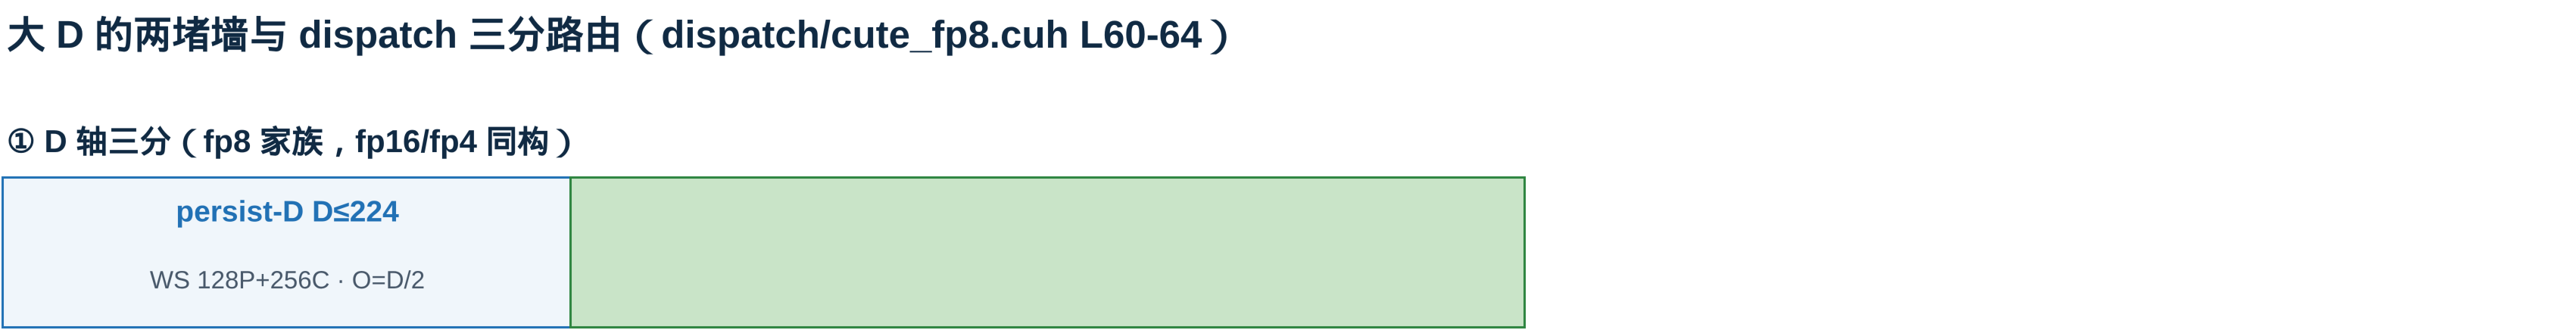
\includegraphics[width=0.98\textwidth]{figures/drawio/fig-30-1-split-d-walls/fig-30-1-split-d-walls.png}
  \begin{tikzpicture}
    \node[anchor=west, inner sep=0pt, align=left, font={\fontsize{7.4}{9.3}\selectfont \bfseries }] at (0.37,-0.354) {大 D 的两堵墙与 dispatch 三分路由（dispatch/cute\_fp8.cuh L60-64）};% w=17.433
    \node[anchor=west, inner sep=0pt, align=left, font={\fontsize{6.1}{7.7}\selectfont \bfseries }] at (0.37,-1.078) {(1) D 轴三分（fp8 家族，fp16/fp4 同构）};% w=4.620
    \node[draw=tkBlue, fill=tkFillBlue, line width=0.5pt, minimum width=3.85cm, minimum height=1.02cm, inner sep=1pt, align=center, text width=3.79cm, font={\fontsize{5.7}{7.1}\selectfont }] at (2.295,-1.833) {};
    \node[anchor=center, inner sep=0pt, align=center, font={\fontsize{5.7}{7.1}\selectfont \bfseries \color{tkBlue} }] at (2.295,-1.555) {persist-D  D$\leq$224};% w=3.665
    \node[anchor=center, inner sep=0pt, align=center, font={\fontsize{4.8}{6.0}\selectfont \color{black!65} }] at (2.295,-2.017) {WS 128P+256C $\cdot$ O=D/2};% w=3.665
    \node[draw=tkGreen, fill=tkFillGreen, line width=0.5pt, minimum width=6.47cm, minimum height=1.02cm, inner sep=1pt, align=center, text width=6.41cm, font={\fontsize{5.7}{7.1}\selectfont }] at (7.454,-1.833) {};
    \node[anchor=center, inner sep=0pt, align=center, font={\fontsize{5.7}{7.1}\selectfont \bfseries \color{tkGreen!70!black} }] at (7.454,-1.555) {split-D M8N1  224$<$D$<$768};% w=6.283
    \node[anchor=center, inner sep=0pt, align=center, font={\fontsize{4.8}{6.0}\selectfont \color{black!65} }] at (7.454,-2.017) {kBr/kBc=128/128 $\cdot$ non-WS 256T $\cdot$ O=D/2};% w=6.283
    \node[draw=tkOrange, fill=tkFillOrange, line width=0.5pt, minimum width=7.39cm, minimum height=1.02cm, inner sep=1pt, align=center, text width=7.33cm, font={\fontsize{5.7}{7.1}\selectfont }] at (13.614,-1.833) {};
    \node[anchor=center, inner sep=0pt, align=center, font={\fontsize{5.7}{7.1}\selectfont \bfseries \color{tkOrange} }] at (13.614,-1.555) {split-D M4N2  D$\geq$768};% w=7.207
    \node[anchor=center, inner sep=0pt, align=center, font={\fontsize{4.8}{6.0}\selectfont \color{black!65} }] at (13.614,-2.017) {kBr/kBc=64/64 $\cdot$ non-WS 256T $\cdot$ O=D/4};% w=7.207
    \node[anchor=center, inner sep=0pt, align=center, font={\fontsize{5.2}{6.6}\selectfont \bfseries }] at (11.15,-1.001) {交叉点 D=768};% w=2.464
    \node[draw=tkRed, fill=tkFillRed, line width=0.5pt, minimum width=8.32cm, minimum height=2.62cm, inner sep=1pt, align=center, text width=8.25cm, font={\fontsize{5.7}{7.1}\selectfont }] at (4.528,-4.235) {};
    \node[anchor=west, inner sep=0pt, align=left, font={\fontsize{6.1}{7.7}\selectfont \bfseries \color{tkRed} }] at (0.616,-3.219) {墙一 smem：K tile 字节 = Bc$\times$D$\times$1B，O(D)};% w=7.823
    \node[anchor=west, inner sep=0pt, align=left, font={\fontsize{5.2}{6.6}\selectfont }] at (0.616,-3.634) {D=512、Bc=128 $\to$ K tile 64KB；加 V stage + Q 即超 99KB 预算};% w=7.823
    \node[anchor=west, inner sep=0pt, align=left, font={\fontsize{5.2}{6.6}\selectfont }] at (0.616,-4.004) {persist-D 的 K stage-0 复用只在 D$\leq$224 挤得过};% w=7.823
    \node[draw=tkRed, fill=none, line width=0.5pt, minimum width=3.70cm, minimum height=0.95cm, inner sep=1pt, align=center, text width=3.63cm, font={\fontsize{5.2}{6.6}\selectfont }] at (2.464,-4.759) {整块 K tile 一次进 smem\\（persist-D：D$\leq$224 专属）};
    \node[draw=tkGreen, fill=none, line width=0.5pt, minimum width=3.70cm, minimum height=0.95cm, inner sep=1pt, align=center, text width=3.63cm, font={\fontsize{5.2}{6.6}\selectfont \bfseries \color{tkGreen!70!black} }] at (6.468,-4.759) {split-D：D 切 chunk 流水\\每 stage 与总 D 无关};
    \node[anchor=west, inner sep=0pt, align=left, font={\fontsize{4.8}{6.0}\selectfont \color{black!55} }] at (0.616,-5.405) {chunk\_index = kv\_tile$\cdot$kDChunks + c，stage/phase 环形推进};% w=7.823
    \node[draw=tkPurple, fill=tkFillPurple, line width=0.5pt, minimum width=8.62cm, minimum height=2.62cm, inner sep=1pt, align=center, text width=8.56cm, font={\fontsize{5.7}{7.1}\selectfont }] at (13.49,-4.235) {};
    \node[anchor=west, inner sep=0pt, align=left, font={\fontsize{6.1}{7.7}\selectfont \bfseries \color{tkPurple} }] at (9.425,-3.219) {墙二 寄存器：O 累加器 = D/(2N\_w) f32/线程};% w=8.131
    \node[anchor=west, inner sep=0pt, align=left, font={\fontsize{5.2}{6.6}\selectfont }] at (9.425,-3.634) {M8N1 单 warp 独占整 D 列：D=512 $\to$ 256 regs 压线（上限 255）};% w=8.131
    \node[anchor=west, inner sep=0pt, align=left, font={\fontsize{5.2}{6.6}\selectfont }] at (9.425,-4.004) {D$\geq$896 大量 spill 崩塌（D=1024 实测 \textasciitilde{}100T）};% w=8.131
    \node[draw=tkPurple, fill=none, line width=0.5pt, minimum width=3.85cm, minimum height=0.95cm, inner sep=1pt, align=center, text width=3.79cm, font={\fontsize{5.2}{6.6}\selectfont }] at (11.35,-4.759) {M8N1 (8,1,1)：O=D/2\\D=1024 $\to$ 512 regs 溢出};
    \node[draw=tkOrange, fill=none, line width=0.5pt, minimum width=3.85cm, minimum height=0.95cm, inner sep=1pt, align=center, text width=3.79cm, font={\fontsize{5.2}{6.6}\selectfont \bfseries \color{tkOrange!75!black} }] at (15.508,-4.759) {M4N2 (4,2,1)：O=D/4\\D=1024 $\to$ 256 regs 边缘 spill 154T};
    \node[draw=gray!55, fill=black!2, line width=0.5pt, minimum width=17.43cm, minimum height=2.31cm, inner sep=1pt, align=center, text width=17.37cm, font={\fontsize{5.7}{7.1}\selectfont }] at (9.086,-7.253) {};
    \node[anchor=west, inner sep=0pt, align=left, font={\fontsize{6.1}{7.7}\selectfont \bfseries }] at (0.616,-6.391) {(2) 寄存器压力模型：N\_w 消去，只有减 M\_w 有效};% w=16.940
    \node[anchor=west, inner sep=0pt, align=left, font={\fontsize{5.7}{7.1}\selectfont }] at (0.616,-6.868) {per-thread：O\_acc = 4$\cdot$(kBr/16M\_w)$\cdot$(D/8N\_w)/(kBr/16M\_w) = D/(2N\_w)};% w=9.856
    \node[anchor=west, inner sep=0pt, align=left, font={\fontsize{5.7}{7.1}\selectfont \bfseries \color{tkPurple} }] at (0.616,-7.269) {per-SM 池占比：[D/(2N\_w)] / [65536/(32M\_wN\_w)] = D$\cdot$M\_w/4096};% w=9.856
    \node[anchor=west, inner sep=0pt, align=left, font={\fontsize{5.2}{6.6}\selectfont \color{black!65} }] at (0.616,-7.669) {N\_w 精确消去：M4N4 $\equiv$ M4N2（同为 D/1024）；M2N4 $\to$ D/2048 是 D$>$1024 正解};% w=9.856
    \node[anchor=west, inner sep=0pt, align=left, font={\fontsize{5.2}{6.6}\selectfont \bfseries \color{tkRed} }] at (10.965,-7.099) {被否决的捷径(1)：QK M8N1 + PV M4N2 混合布局};% w=6.591
    \node[anchor=west, inner sep=0pt, align=left, font={\fontsize{4.8}{6.0}\selectfont }] at (10.965,-7.623) {QK/PV 共享 Q tile，M 维须一致：\\kBr=128 $\to$ PV 仍 D/2\\kBr=64 $\to$ M8N1 空 4 warp};% w=6.591
    \node[anchor=west, inner sep=0pt, align=left, font={\fontsize{5.2}{6.6}\selectfont \bfseries \color{tkRed} }] at (10.965,-8.177) {被否决的捷径(2)：WS 版 split-D};% w=6.591
    \node[anchor=west, inner sep=0pt, align=left, font={\fontsize{4.8}{6.0}\selectfont }] at (10.965,-8.747) {setmaxnreg 上限 232 装不下 D=512 的 256-reg O};% w=6.591
    \node[draw=tkGreen, fill=tkFillGreen, line width=0.5pt, minimum width=17.43cm, minimum height=2.31cm, inner sep=1pt, align=center, text width=17.37cm, font={\fontsize{5.7}{7.1}\selectfont }] at (9.086,-10.025) {};
    \node[anchor=west, inner sep=0pt, align=left, font={\fontsize{6.1}{7.7}\selectfont \bfseries \color{tkGreen!70!black} }] at (0.616,-9.163) {(3) 实测交叉点（5090，fp16 同构；PRO 5000 数据见正文 30.6）};% w=16.940
    \node[anchor=west, inner sep=0pt, align=left, font={\fontsize{5.2}{6.6}\selectfont }] at (0.616,-9.579) {D$\leq$640：M8N1 快 +2\textasciitilde{}16\%（无 P roundtrip、kBr 大一倍）};% w=8.316
    \node[anchor=west, inner sep=0pt, align=left, font={\fontsize{5.2}{6.6}\selectfont \bfseries }] at (0.616,-9.948) {D$\geq$768：M4N2 快 +7\%@768、+11\%@896、+55\%@1024};% w=8.316
    \node[anchor=west, inner sep=0pt, align=left, font={\fontsize{5.2}{6.6}\selectfont \color{black!55} }] at (0.616,-10.318) {FFPA\_FP8\_FORCE\_KERNEL=split\_d|m4n2（224$<$D$\leq$1024）可强制 A/B};% w=8.316
    \node[anchor=west, inner sep=0pt, align=left, font={\fontsize{5.2}{6.6}\selectfont \color{black!55} }] at (0.616,-10.688) {PRO 5000 实测（本机 headdim 止于 512）：D=512 self 203T / 2.98x};% w=8.316
    \node[anchor=west, inner sep=0pt, align=left, font={\fontsize{5.7}{7.1}\selectfont \bfseries \color{tkGreen!70!black} }] at (9.548,-9.579) {split-D 是精确变换：};% w=8.008
    \node[anchor=west, inner sep=0pt, align=left, font={\fontsize{5.2}{6.6}\selectfont }] at (9.548,-9.948) {QK 侧 D 是归约维：$\Sigma$\_c Q\_c K\_c\^{}T 累加进同一 S（无新舍入点）};% w=8.008
    \node[anchor=west, inner sep=0pt, align=left, font={\fontsize{5.2}{6.6}\selectfont }] at (9.548,-10.318) {PV 侧 D 是输出列维：各 chunk 的 O 段独立累加};% w=8.008
    \node[anchor=west, inner sep=0pt, align=left, font={\fontsize{5.2}{6.6}\selectfont \bfseries }] at (9.548,-10.688) {softmax 行统计 (m,$\ell$) 是 KV 行维的量------与 D 切分无关};% w=8.008
    \draw[black!75, line width=0.8pt, dashed] (9.918,-1.14) -- (9.918,-2.464);
    \draw[gray!55, line width=0.5pt, dashed] (4.22,-1.14) -- (4.22,-2.464);
    \draw[tkGreen, line width=0.8pt, -{Stealth[length=2.2pt,width=1.8pt]}] (4.312,-4.759) -- (4.62,-4.759);
    \draw[tkOrange, line width=0.8pt, -{Stealth[length=2.2pt,width=1.8pt]}] (13.275,-4.759) -- (13.583,-4.759);
    \draw[gray!55, line width=0.5pt] (10.718,-6.714) -- (10.718,-8.1);
    \draw[gray!55, line width=0.5pt] (9.302,-9.425) -- (9.302,-10.842);
  \end{tikzpicture}
  \caption{大 $D$ 的两堵墙与 dispatch 三分路由。smem 墙由 split-D 拆
  （chunk 流水，smem 与 $D$ 解耦）；寄存器墙由 M4N2 拆（$N_w=2$ 把
  per-thread $O$ 从 $D/2$ 减到 $D/4$）；$D=768$ 是实测交叉点。}
  \label{fig:30-walls}
\end{figure}

\begin{figure}[htbp]
  \centering
  % was: 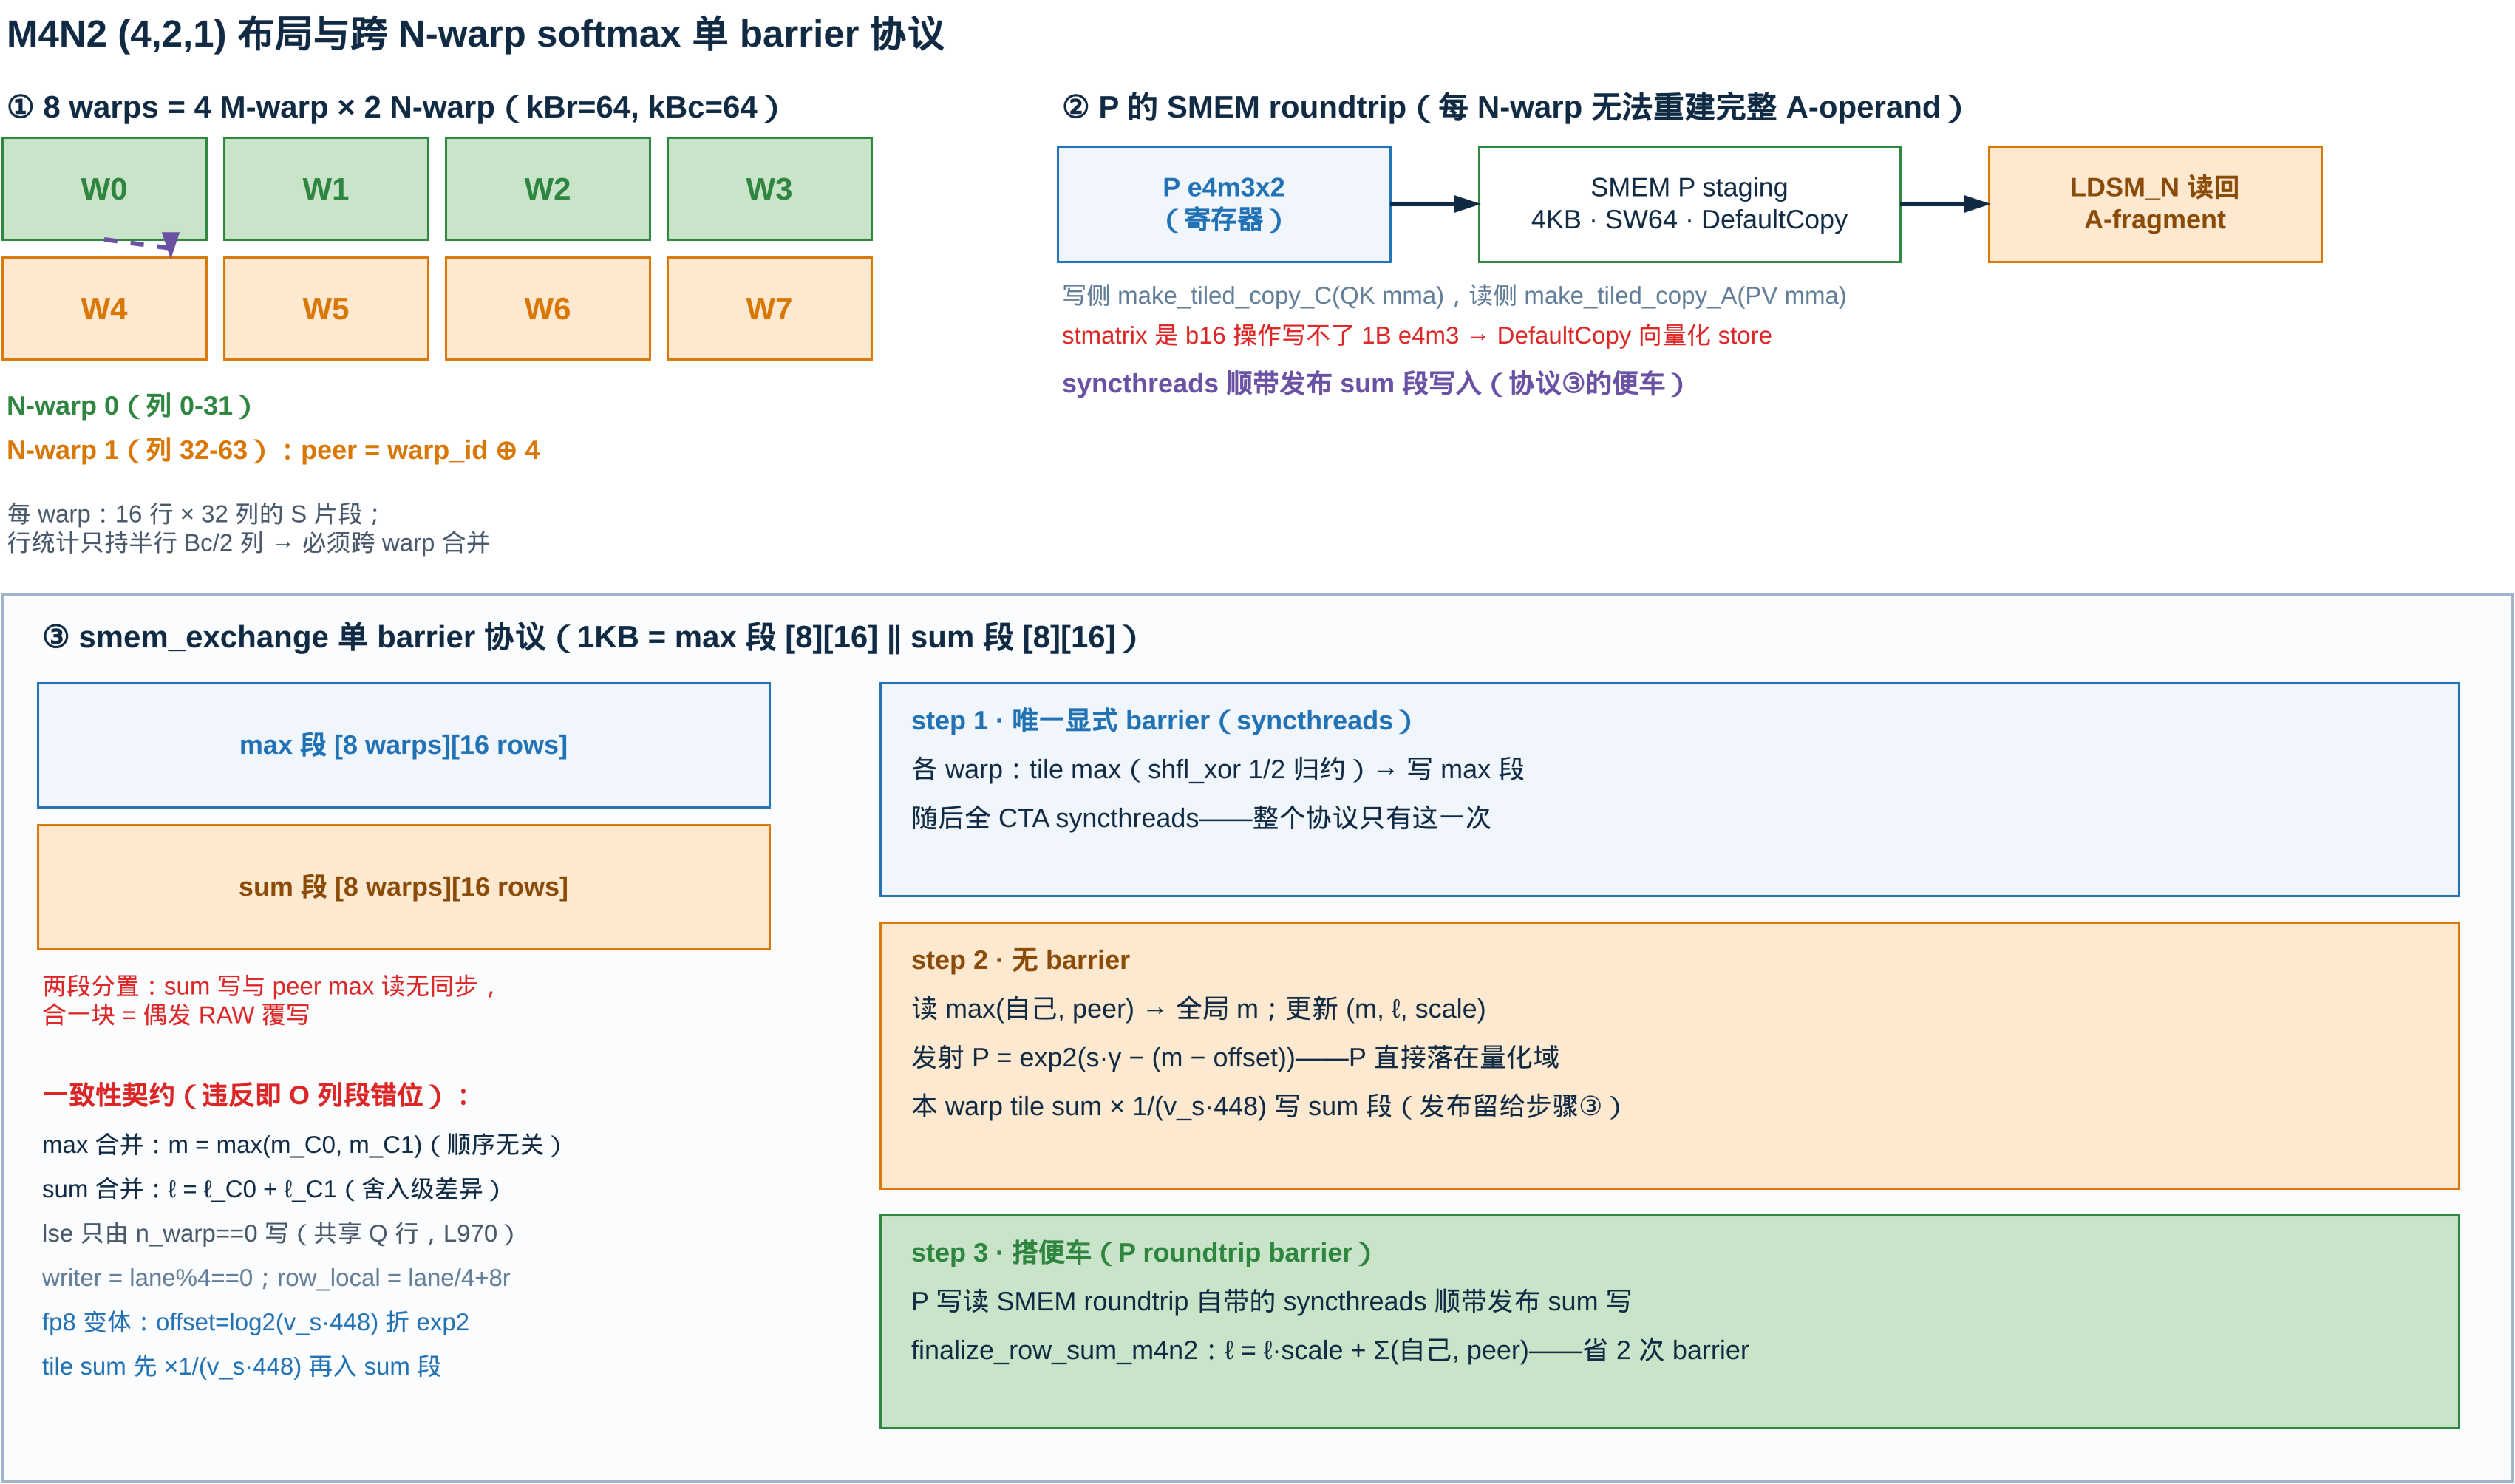
\includegraphics[width=0.98\textwidth]{figures/drawio/fig-30-2-m4n2-softmax/fig-30-2-m4n2-softmax.png}
  \begin{tikzpicture}
    \node[anchor=west, inner sep=0pt, align=left, font={\fontsize{7.4}{9.3}\selectfont \bfseries }] at (0.37,-0.354) {M4N2 (4,2,1) 布局与跨 N-warp softmax 单 barrier 协议};% w=17.433
    \node[anchor=west, inner sep=0pt, align=left, font={\fontsize{5.6}{7.0}\selectfont \bfseries }] at (0.37,-0.862) {(1) 8 warps = 4 M-warp $\times$ 2 N-warp（kBr=64, kBc=64）};% w=8.624
    \node[draw=tkGreen, fill=tkFillGreen, line width=0.5pt, minimum width=1.42cm, minimum height=0.71cm, inner sep=1pt, align=center, text width=1.36cm, font={\fontsize{6.1}{7.7}\selectfont \bfseries \color{tkGreen!70!black} }] at (1.078,-1.432) {W0};
    \node[draw=tkGreen, fill=tkFillGreen, line width=0.5pt, minimum width=1.42cm, minimum height=0.71cm, inner sep=1pt, align=center, text width=1.36cm, font={\fontsize{6.1}{7.7}\selectfont \bfseries \color{tkGreen!70!black} }] at (2.618,-1.432) {W1};
    \node[draw=tkGreen, fill=tkFillGreen, line width=0.5pt, minimum width=1.42cm, minimum height=0.71cm, inner sep=1pt, align=center, text width=1.36cm, font={\fontsize{6.1}{7.7}\selectfont \bfseries \color{tkGreen!70!black} }] at (4.158,-1.432) {W2};
    \node[draw=tkGreen, fill=tkFillGreen, line width=0.5pt, minimum width=1.42cm, minimum height=0.71cm, inner sep=1pt, align=center, text width=1.36cm, font={\fontsize{6.1}{7.7}\selectfont \bfseries \color{tkGreen!70!black} }] at (5.698,-1.432) {W3};
    \node[draw=tkOrange, fill=tkFillOrange, line width=0.5pt, minimum width=1.42cm, minimum height=0.71cm, inner sep=1pt, align=center, text width=1.36cm, font={\fontsize{6.1}{7.7}\selectfont \bfseries \color{tkOrange} }] at (1.078,-2.264) {W4};
    \node[draw=tkOrange, fill=tkFillOrange, line width=0.5pt, minimum width=1.42cm, minimum height=0.71cm, inner sep=1pt, align=center, text width=1.36cm, font={\fontsize{6.1}{7.7}\selectfont \bfseries \color{tkOrange} }] at (2.618,-2.264) {W5};
    \node[draw=tkOrange, fill=tkFillOrange, line width=0.5pt, minimum width=1.42cm, minimum height=0.71cm, inner sep=1pt, align=center, text width=1.36cm, font={\fontsize{6.1}{7.7}\selectfont \bfseries \color{tkOrange} }] at (4.158,-2.264) {W6};
    \node[draw=tkOrange, fill=tkFillOrange, line width=0.5pt, minimum width=1.42cm, minimum height=0.71cm, inner sep=1pt, align=center, text width=1.36cm, font={\fontsize{6.1}{7.7}\selectfont \bfseries \color{tkOrange} }] at (5.698,-2.264) {W7};
    \node[anchor=west, inner sep=0pt, align=left, font={\fontsize{5.2}{6.6}\selectfont \bfseries \color{tkGreen!70!black} }] at (0.37,-2.941) {N-warp 0（列 0-31）};% w=6.406
    \node[anchor=west, inner sep=0pt, align=left, font={\fontsize{5.2}{6.6}\selectfont \bfseries \color{tkOrange} }] at (0.37,-3.249) {N-warp 1（列 32-63）：peer = warp\_id $\oplus$ 4};% w=6.406
    \node[anchor=west, inner sep=0pt, align=left, font={\fontsize{4.8}{6.0}\selectfont \color{black!65} }] at (0.37,-3.788) {每 warp：16 行 $\times$ 32 列的 S 片段；\\行统计只持半行 Bc/2 列 $\to$ 必须跨 warp 合并};% w=6.622
    \node[anchor=west, inner sep=0pt, align=left, font={\fontsize{6.1}{7.7}\selectfont \bfseries }] at (7.7,-0.862) {(2) P 的 SMEM roundtrip（每 N-warp 无法重建完整 A-operand）};% w=10.102
    \node[draw=tkBlue, fill=tkFillBlue, line width=0.5pt, minimum width=2.31cm, minimum height=0.80cm, inner sep=1pt, align=center, text width=2.25cm, font={\fontsize{5.2}{6.6}\selectfont \bfseries \color{tkBlue} }] at (8.855,-1.54) {P e4m3x2\\（寄存器）};
    \node[draw=tkGreen, fill=none, line width=0.5pt, minimum width=2.93cm, minimum height=0.80cm, inner sep=1pt, align=center, text width=2.86cm, font={\fontsize{5.0}{6.3}\selectfont }] at (12.089,-1.54) {SMEM P staging\\4KB $\cdot$ SW64 $\cdot$ DefaultCopy};
    \node[draw=tkOrange, fill=tkFillOrange, line width=0.5pt, minimum width=2.31cm, minimum height=0.80cm, inner sep=1pt, align=center, text width=2.25cm, font={\fontsize{5.2}{6.6}\selectfont \bfseries \color{tkOrange!75!black} }] at (15.323,-1.54) {LDSM\_N 读回\\A-fragment};
    \node[anchor=west, inner sep=0pt, align=left, font={\fontsize{4.8}{6.0}\selectfont \color{black!55} }] at (7.7,-2.171) {写侧 make\_tiled\_copy\_C(QK mma)，读侧 make\_tiled\_copy\_A(PV mma)};% w=8.778
    \node[anchor=west, inner sep=0pt, align=left, font={\fontsize{4.8}{6.0}\selectfont \color{tkRed} }] at (7.7,-2.449) {stmatrix 是 b16 操作写不了 1B e4m3 $\to$ DefaultCopy 向量化 store};% w=8.778
    \node[anchor=west, inner sep=0pt, align=left, font={\fontsize{5.2}{6.6}\selectfont \bfseries \color{tkPurple} }] at (7.7,-2.787) {syncthreads 顺带发布 sum 段写入（协议(3)的便车）};% w=8.778
    \node[draw=gray!55, fill=black!2, line width=0.5pt, minimum width=17.43cm, minimum height=6.16cm, inner sep=1pt, align=center, text width=17.37cm, font={\fontsize{5.7}{7.1}\selectfont }] at (9.086,-7.33) {};
    \node[anchor=west, inner sep=0pt, align=left, font={\fontsize{6.1}{7.7}\selectfont \bfseries }] at (0.616,-4.543) {(3) smem\_exchange 单 barrier 协议（1KB = max 段 [8][16] $\|$ sum 段 [8][16]）};% w=16.940
    \node[draw=tkBlue, fill=tkFillBlue, line width=0.5pt, minimum width=5.08cm, minimum height=0.86cm, inner sep=1pt, align=center, text width=5.02cm, font={\fontsize{5.2}{6.6}\selectfont \bfseries \color{tkBlue} }] at (3.157,-5.298) {max 段 [8 warps][16 rows]};
    \node[draw=tkOrange, fill=tkFillOrange, line width=0.5pt, minimum width=5.08cm, minimum height=0.86cm, inner sep=1pt, align=center, text width=5.02cm, font={\fontsize{5.2}{6.6}\selectfont \bfseries \color{tkOrange!75!black} }] at (3.157,-6.283) {sum 段 [8 warps][16 rows]};
    \node[anchor=west, inner sep=0pt, align=left, font={\fontsize{4.8}{6.0}\selectfont \color{tkRed} }] at (0.616,-7.069) {两段分置：sum 写与 peer max 读无同步，\\合一块 = 偶发 RAW 覆写};% w=5.174
    \node[anchor=west, inner sep=0pt, align=left, font={\fontsize{5.2}{6.6}\selectfont \bfseries \color{tkRed} }] at (0.616,-7.731) {一致性契约（违反即 O 列段错位）：};% w=5.236
    \node[anchor=west, inner sep=0pt, align=left, font={\fontsize{4.8}{6.0}\selectfont }] at (0.616,-8.07) {max 合并：m = max(m\_C0, m\_C1)（顺序无关）};% w=5.236
    \node[anchor=west, inner sep=0pt, align=left, font={\fontsize{4.8}{6.0}\selectfont }] at (0.616,-8.378) {sum 合并：$\ell$ = $\ell$\_C0 + $\ell$\_C1（舍入级差异）};% w=5.236
    \node[anchor=west, inner sep=0pt, align=left, font={\fontsize{4.8}{6.0}\selectfont \color{black!65} }] at (0.616,-8.686) {lse 只由 n\_warp==0 写（共享 Q 行，L970）};% w=5.236
    \node[anchor=west, inner sep=0pt, align=left, font={\fontsize{4.8}{6.0}\selectfont \color{black!55} }] at (0.616,-8.994) {writer = lane\%4==0；row\_local = lane/4+8r};% w=5.236
    \node[anchor=west, inner sep=0pt, align=left, font={\fontsize{4.8}{6.0}\selectfont \color{tkBlue} }] at (0.616,-9.302) {fp8 变体：offset=log2(v\_s$\cdot$448) 折 exp2};% w=5.236
    \node[anchor=west, inner sep=0pt, align=left, font={\fontsize{4.8}{6.0}\selectfont \color{tkBlue} }] at (0.616,-9.61) {tile sum 先 $\times$1/(v\_s$\cdot$448) 再入 sum 段};% w=5.236
    \node[draw=tkBlue, fill=tkFillBlue, line width=0.5pt, minimum width=10.96cm, minimum height=1.48cm, inner sep=1pt, align=center, text width=10.90cm, font={\fontsize{5.7}{7.1}\selectfont }] at (11.95,-5.606) {};
    \node[anchor=west, inner sep=0pt, align=left, font={\fontsize{5.2}{6.6}\selectfont \bfseries \color{tkBlue} }] at (6.653,-5.128) {step 1 $\cdot$ 唯一显式 barrier（syncthreads）};% w=10.595
    \node[anchor=west, inner sep=0pt, align=left, font={\fontsize{5.2}{6.6}\selectfont }] at (6.653,-5.467) {各 warp：tile max（shfl\_xor 1/2 归约）$\to$ 写 max 段};% w=10.595
    \node[anchor=west, inner sep=0pt, align=left, font={\fontsize{5.2}{6.6}\selectfont }] at (6.653,-5.806) {随后全 CTA syncthreads------整个协议只有这一次};% w=10.595
    \node[draw=tkOrange, fill=tkFillOrange, line width=0.5pt, minimum width=10.96cm, minimum height=1.85cm, inner sep=1pt, align=center, text width=10.90cm, font={\fontsize{5.7}{7.1}\selectfont }] at (11.95,-7.454) {};
    \node[anchor=west, inner sep=0pt, align=left, font={\fontsize{5.2}{6.6}\selectfont \bfseries \color{tkOrange!75!black} }] at (6.653,-6.791) {step 2 $\cdot$ 无 barrier};% w=10.595
    \node[anchor=west, inner sep=0pt, align=left, font={\fontsize{5.2}{6.6}\selectfont }] at (6.653,-7.13) {读 max(自己, peer) $\to$ 全局 m；更新 (m, $\ell$, scale)};% w=10.595
    \node[anchor=west, inner sep=0pt, align=left, font={\fontsize{5.2}{6.6}\selectfont }] at (6.653,-7.469) {发射 P = exp2(s$\cdot$$\gamma$ $-$ (m $-$ offset))------P 直接落在量化域};% w=10.595
    \node[anchor=west, inner sep=0pt, align=left, font={\fontsize{5.2}{6.6}\selectfont }] at (6.653,-7.808) {本 warp tile sum $\times$ 1/(v\_s$\cdot$448) 写 sum 段（发布留给步骤(3)）};% w=10.595
    \node[draw=tkGreen, fill=tkFillGreen, line width=0.5pt, minimum width=10.96cm, minimum height=1.48cm, inner sep=1pt, align=center, text width=10.90cm, font={\fontsize{5.7}{7.1}\selectfont }] at (11.95,-9.302) {};
    \node[anchor=west, inner sep=0pt, align=left, font={\fontsize{5.2}{6.6}\selectfont \bfseries \color{tkGreen!70!black} }] at (6.653,-8.824) {step 3 $\cdot$ 搭便车（P roundtrip barrier）};% w=10.595
    \node[anchor=west, inner sep=0pt, align=left, font={\fontsize{5.2}{6.6}\selectfont }] at (6.653,-9.163) {P 写读 SMEM roundtrip 自带的 syncthreads 顺带发布 sum 写};% w=10.595
    \node[anchor=west, inner sep=0pt, align=left, font={\fontsize{5.2}{6.6}\selectfont }] at (6.653,-9.502) {finalize\_row\_sum\_m4n2：$\ell$ = $\ell$$\cdot$scale + $\Sigma$(自己, peer)------省 2 次 barrier};% w=10.595
    \draw[tkPurple, line width=0.8pt, dashed, -{Stealth[length=2.2pt,width=1.8pt]}] (1.078,-1.786) -- (1.54,-1.848) -- (1.54,-1.91);
    \draw[black!75, line width=0.8pt, -{Stealth[length=2.2pt,width=1.8pt]}] (10.01,-1.54) -- (10.626,-1.54);
    \draw[black!75, line width=0.8pt, -{Stealth[length=2.2pt,width=1.8pt]}] (13.552,-1.54) -- (14.168,-1.54);
  \end{tikzpicture}
  \caption{M4N2 的 $(4,2,1)$ atom 布局与跨 N-warp softmax 单 barrier
  协议。max 段与 sum 段分置 \texttt{smem\_exchange} 防 RAW；sum 的
  发布搭 P roundtrip barrier 的便车。}
  \label{fig:30-m4n2}
\end{figure}

\FloatBarrier

\section{性能分析}

\subsection{本机实测（RTX PRO 5000，B1 H32 N8192，bench 默认配置）}

命令：
\begin{lstlisting}[style=console,aboveskip=4pt,belowskip=2pt]
export CUDA_VISIBLE_DEVICES=7 FFPA_CUDA_ALLOW_SMALL_D=1
python -m ffpa_attn.bench --fwd-backend cuda --cuda-impl fp8 \
  --tasks self-attn,causal --D {256,320,512} --no-bwd --show-allclose
\end{lstlisting}

\begin{center}
\begin{tabular}{@{}llrrrl@{}}
\toprule
$D$ & task & FFPA ms & SDPA ms & TFLOPS & speedup \\
\midrule
256 & self   & 8.12  & 10.52 & 271T & 1.30x \\
256 & causal & 4.73  & 5.29  & 233T & 1.12x \\
320 & self   & 10.71 & 40.25 & 257T & 3.76x \\
320 & causal & 6.23  & 20.61 & 221T & 3.31x \\
512 & self   & 21.71 & 64.74 & 203T & 2.98x \\
512 & causal & 12.82 & 32.92 & 172T & 2.57x \\
\bottomrule
\end{tabular}
\end{center}

三条读数：其一，self-attn 的 speedup 从 $D=256$ 的 1.30x 跳到
$D=320$ 的 3.76x——拐点不在 kernel 而在\textbf{参照系}：SDPA 在
$D\notin\{64,128\}$ 时掉出最优 kernel 选择，fp8 的 1B 元素带宽优势
立即显形。其二，TFLOPS 随 $D$ 单调下降（271$\to$203T）：$D$ 越大
softmax 与 P 量化等 $O(B_c)$ 项占比越高、$O$ 寄存器压力越大，这是
split-D 无法消除的税。其三，causal 的 allclose 在 D=320 bf16 与
D=512 fp16 两格临界失败——见 30.2.3~节的已知边界说明；dense 六格
全绿，数据落盘 \texttt{.tmp/book-bench/ch30/}。

\subsection{交叉点与 M4N2 的引用数据（本机无 $D\ge768$ 编译实例）}

本机 headdim 编译集止于 512，M4N2 只能引用 5090 数据（fp16 家族同构、
同一 dispatch 交叉点）：$D\le640$ 时 M8N1 快 $2\sim16\%$；
$D\ge768$ 时 M4N2 快 $+7\%@768$、$+11\%@896$、$+55\%@1024$。崩塌侧
的数字更有教学价值：$D=1024$ 时 M8N1 的 $O_{\text{acc}}=512$ regs
溢出 local memory，吞吐 $\sim$100T；M4N2 同 $D$ 边缘 spill 仍有
154T。\texttt{FFPA\_FP8\_FORCE\_KERNEL=split\_d|m4n2}（$224<D\le1024$，
\texttt{dispatch/cute\_fp8.cuh} L24--33，仅在 \texttt{--debug-ext fp8}
的 debug 构建里生效）可在有 768+ 编译实例的
机器上强制 A/B 复现交叉点。

\subsection{roofline 视角}

fp8 split-D 在 $D=512$ 的 203T 大约是 fp8 persist-D 峰值（365T，
表~29.2）的 56\%。差价的构成：$O$ 累加器随 $D$ 翻倍的寄存器税
（occupancy 1 CTA）、chunk 循环多出的 barrier 握手、以及 epilogue
批量 staging 的 smem 往返。这不是 split-D 的失败——绝对吞吐仍高于
fp16 家族同 $D$ 量级，带宽侧（1B/元素）更是 3.76x speedup 的直接
来源。

\section{实践经验}

\subsection{案例：causal allclose 临界失败的定位与定性}

30.6~节表格里有两格 \texttt{allclose} 失败：D=320（bf16）、
D=512（fp16）。

定性过程值得记录，脚本在 \texttt{.tmp/book-bench/ch30/}：

\begin{enumerate}[itemsep=0pt,topsep=2pt]
  \item \textbf{先看模式不看标量}。对 $D\in\{256,320,512\}$ 各跑
        causal，逐 512-行块统计超阈行占比：三者模式\textbf{完全一致}
        ——前 $\sim$30\% 块 100\% 超阈、后段 0\%，max $\sim$2、
        mean $\sim$0.007；
  \item \textbf{dense 对照}。self-attn 六格全绿 $\Rightarrow$ 排除
        kernel 结构性错误（chunk 流水、mask、epilogue 都对）；
  \item \textbf{对照头注释}。L40--43 声明的「causal 早期行
        attend 少、误差不被平均」与实测模式吻合：早期行
        $P$ 分布尖，e4m3 的 $2^{-3}$ 相对舍入直接进 $O$；行号
        过半后 $P$ 足够平，误差被平均掉；
  \item \textbf{结论}：已知精度特性，非回归 bug。需要严格
        causal 精度的场景走 hybrid（前若干行 fp16 stage-1）。
\end{enumerate}

这套流程（模式 $\to$ dense 对照 $\to$ 对照声明 $\to$ 定性）与
29.7.1~节 D=192 的五步法同构：先证明「不是 bug」再决定要不要修。

\subsection{什么时候不该学本章}

split-D/M4N2 是 $D>224$ 的\textbf{被迫选择}，不是普适更优。三条负面
证据：WS 版 split-D 被 setmaxnreg 232 上限否决；QK/PV 混合 atom 布局
被 M 维一致性否决；fused-rescale 在 split-D 域被单 CTA 藏不住的
tensor pipe 压力否决。三条都是「在 persist-D 域成立的优化不能平移」
的实例——迁移优化前先核对 occupancy 与寄存器结构是否同型。

\section{常见坑}

\begin{enumerate}[itemsep=2pt,topsep=2pt]
  \item \textbf{P roundtrip 写侧坐标系}：写侧必须从 QK 的
        \texttt{tiled\_mma\_qk} 构造 \texttt{make\_tiled\_copy\_C}，
        读侧从 PV 的 \texttt{tiled\_mma\_pv} 构造
        \texttt{make\_tiled\_copy\_A}；手写 A-operand 映射与 LDSM
        读侧不对称会数值爆炸（sm80 家族血泪，L685--698 用
        \texttt{DefaultCopy} 规避向量化陷阱）。
  \item \textbf{max/sum 同区覆写}：单 barrier 协议里 sum 写与 peer
        max 读之间没有同步，两段必须分置；合成一块省下的 512B 换来
        偶发 RAW 错值（softmax.cuh L92--95）。
  \item \textbf{stmatrix 写不了 1B e4m3}：它是 b16 操作；1B 元素的
        P staging 退回 \texttt{DefaultCopy} 向量化 store（L685--688）。
  \item \textbf{两套块宽不一致}：$k_{Br}=64$ vs 量化 128 行块，奇数
        tile 需要 \texttt{quant\_offset}/\texttt{quant\_rb} 重映射
        （L129、L300--307）；漏掉的行查到邻块的 scale，误差温和到
        很难肉眼发现。
  \item \textbf{kSmemElems 的单位}：fp8 traits 里它数 1B 元素恰等于
        字节数；O staging 断言要乘 \texttt{sizeof(ElementO)}，否则
        预算虚大一倍（L105--108）。
  \item \textbf{stage 下限的家族差异}：persist-D 抬 stages 已证伪、
        m4n2 抬到 3 是全局最优——差别只在 occupancy 是否已被锁死；
        跨家族抄 stage 配置前先想清楚这一条。
\end{enumerate}

\section{面试要点速查}

\begin{enumerate}[itemsep=2pt,topsep=2pt]
  \item \textbf{split-D 为什么精确}？QK 侧 $D$ 是归约维，chunk 累加
        进同一 fragment（式~\ref{eq:30-qk-split}）；PV 侧是输出列维，
        各 chunk 独立（式~\ref{eq:30-pv-split}）；softmax 行统计与
        $D$ 切分无关——不产生 per-chunk 的 $(m,\ell)$。
  \item \textbf{M4N2 减的是哪一维}？$N$ 维（输出列劈 2 warp），
        per-thread $O$ 从 $D/2$ 到 $D/4$；但 per-SM 池占比
        $D\cdot M_w/4096$ 里 $N_w$ 消去（式~\ref{eq:30-smpool}），
        只有减 $M_w$ 才降总量——所以 $D>1024$ 的正解是 M2N4。
  \item \textbf{跨 N-warp softmax 协议}？max 段交换 + 单 barrier；
        sum 搭 P roundtrip barrier 的便车由 \texttt{finalize} 折叠；
        两 N-warp 必须持有相同 $(m,\ell)$ 否则 rescale 因子分裂。
  \item \textbf{P 为什么要过 SMEM}？M4N2 每 N-warp 只持半行
        $B_c$ 列，A-operand 无法 warp 内重建；roundtrip 4KB/tile。
  \item \textbf{交叉点为何在 $D=768$}？之下 M8N1 无 roundtrip 且
        $k_{Br}=128$ 效率高；之上 $D/2$ 逼近/超过 255 寄存器上限，
        M4N2 的 $D/4$ 开始统治（5090：+7\%@768 $\to$ +55\%@1024）。
  \item \textbf{split-D 为何非 WS}？setmaxnreg consumer 上限 232
        装不下 $D\ge512$ 的 256-reg $O$ 累加器；全线程 MMA +
        tid==0 发 TMA 是被迫也是合理。
  \item \textbf{fp8 causal 早期行为何误差大}？attend 的 key 少，
        $P$ 分布尖，e4m3 相对舍入不被平均；dense 无此问题；
        工程解法是 hybrid 前若干行 fp16。
\end{enumerate}

\section{最小测试与动手实验}

\begin{enumerate}[itemsep=2pt,topsep=2pt]
  \item \textbf{bench 复跑}（卡 7）：30.6~节命令逐 $D$ 复现表格；
        观察 self speedup 在 $D=256\to320$ 的跳变并解释参照系切换。
  \item \textbf{误差模式复现}：用 \texttt{CUDABackend(enable\_fp8=True)}
        直接调 \texttt{ffpa\_attn\_func}，对 causal 输出按 512-行块
        统计超阈行占比，画出前 30\% 块 100\% 的直方图
        （\texttt{.tmp/book-bench/ch30/d512\_causal\_check.py}）。
  \item \textbf{stage 扫描}：\texttt{FFPA\_FP8\_KV\_STAGES="K,V"} 组合
        重跑 $D=320$ self，验证 s3 附近的最优与 s4+ 的非单调。
  \item \textbf{A/B 强制}（需 768+ headdim 编译实例的机器，
        且需 \texttt{--debug-ext fp8} 的 debug 构建）：设
        \texttt{FFPA\_FP8\_\allowbreak FORCE\_KERNEL} 为
        \texttt{split\_d} 或 \texttt{m4n2}，
        跑 $D\in\{512,768,1024\}$，复现交叉点与 D=1024 的
        崩塌/边缘 spill 对比。
\end{enumerate}

\section*{延伸阅读}
\addcontentsline{toc}{section}{延伸阅读}

\begin{itemize}[itemsep=0pt,topsep=2pt]
  \item \texttt{cute/fp8/sm\_120/split\_d.cuh} 头注释（L17--44）：
        non-WS 设计声明与 causal 精度边界；
  \item \texttt{cute/softmax.cuh} L74--163：单 barrier 协议与 RAW
        分区的原始注释；
  \item ffpa-cuda-understand skill \S11.3--\S11.4：双墙模型与
        寄存器压力表的完整版（含 fp4 家族对照）；
  \item \texttt{launch/cute\_fp8\_split\_d\_m4n2.cuh} L127--133 与
        PC-8 记录：stage floor 的 NCU 证据链。
\end{itemize}

% ch31-fp4-nvfp4-quant.tex — FP4(一)：NVFP4 格式与量化链（RFC-K5）
% 源码：ffpa-attn(861d75e) cute/fp4/{quantize_fp4(1642L),delta_s(451L),fp4_gemm(276L),attn_traits(658L)}.cuh
\chapter{FP4（一）：NVFP4 格式与量化链}\label{ch:31}

\section{本章导读}

第~\ref{ch:27}--\ref{ch:29}~章建立了量化注意力的数学与 fp8 实现链。
本章把数据格式推到极限——4 bit。NVFP4 不是「把 fp8 的量化代码换个
dtype」：e2m1 只有 2 bit 指数 + 1 bit 尾数，可表示值只有
$\{0,\pm0.5,\pm1,\pm1.5,\pm2,\pm3,\pm4,\pm6\}$，相对步长约 25\%（fp8 e4m3
是 6.25\%）。在这样的格式上做出可用的 attention，靠的不是数据格式本身，
而是围绕它的一整套\textbf{尺度工程}：microscaling 块尺度（scale
factor）、强制 smoothing、rank-1 修正、列置换、以及把所有这些步骤
fused 进尽量少的 kernel。
\begin{figure}[H]
\centering
\begin{tikzpicture}[font=\scriptsize]
  \def\us{2.2}
  \node[anchor=east, align=right] at (-0.35,0.25) {e4m3\\{\tiny 4E+3M}};
  \draw[thick] (0,0) -- ({6*\us},0);
  \draw[thick, ->] ({6*\us},0) -- ({6*\us+0.45},0);
  \foreach \bi in {0,...,7}{
    \foreach \m in {0,...,7}{
      \pgfmathsetmacro{\vv}{2^(\bi-6)*(1+\m/8)}
      \draw[gray!45] ({\vv*\us},0) -- ({\vv*\us},0.5);
    }
  }
  \foreach \m in {0,...,4}{
    \pgfmathsetmacro{\vv}{4+0.5*\m}
    \draw[gray!45] ({\vv*\us},0) -- ({\vv*\us},0.5);
  }
  \foreach \vl/\xx in {0/0,1/2.2,2/4.4,4/8.8,6/13.2}{
    \draw[thick] (\xx,0) -- (\xx,-0.14);
    \node[below, font=\tiny, inner sep=1pt] at (\xx,-0.14) {$\vl$};
  }
  \node[anchor=west, font=\tiny] at ({6*\us+0.55},0.02) {$\to\ \cdots\ 448$（满量程）};
  \node[anchor=south, font=\tiny, align=center] at ({3*\us},0.58)
    {格点密（每 binade 8 点），相对步长 6.25\%；\\无 $\pm\infty$（\texttt{0x7F}=\texttt{NaN}），越界 \texttt{satfinite} 饱和};
  \begin{scope}[yshift=-2.4cm]
    \node[anchor=east, align=right] at (-0.35,0.30) {e2m1\\{\tiny 2E+1M}};
    \draw[thick] (0,0) -- ({6*\us},0);
    \draw[thick, ->] ({6*\us},0) -- ({6*\us+0.45},0);
    \foreach \vl/\xx in {0/0,0.5/1.1,1/2.2,1.5/3.3,2/4.4,3/6.6,4/8.8,6/13.2}{
      \draw[very thick] (\xx,0) -- (\xx,0.62);
      \node[above, font=\tiny, inner sep=1pt] at (\xx,0.64) {\vl};
    }
    \node[anchor=south, font=\tiny, align=center] at ({3*\us},0.78)
      {16 个码点中正半轴（含 0）仅 8 个，相对步长 $\approx$25\%\\格距 0.5/0.5/0.5/1/1/2 逐级加倍};
    \foreach \gx/\gl in {0.55/0.5,1.65/0.5,2.75/0.5,3.85/1,5.5/1,7.7/2}{
      \node[below, font=\tiny, inner sep=1pt] at (\gx,-0.16) {\gl};
    }
    \draw[thick] (8.8,-0.74) -- (8.8,-0.90) -- (13.2,-0.90) -- (13.2,-0.74);
    \node[below, font=\tiny, inner sep=1pt] at (11.0,-0.92) {最大相对间距（4$\to$6，+50\%）};
  \end{scope}
  \node[anchor=north west, align=left, text width=15.2cm, font=\tiny] at (0,-4.15)
    {两格式均有 $\pm0$，负半轴镜像对称（图示正半轴 $[0,6]$）。e2m1 无
     \texttt{inf}/\texttt{NaN}，越界由 \texttt{cvt.rn.satfinite.e2m1x2.f32} 饱和到
     $\pm6$。格点稀疏度 25\% vs 6.25\% 正是 fp4 容差（dense 0.15 / causal 0.70）比
     fp8（5e-2）宽一个量级、以及 causal 尖峰行 max\_abs 0.5--0.75 的直接来源
     （第~\ref{ch:33}~章 33.3.3~节的 tol 分档依据）。};
\end{tikzpicture}
\caption{e2m1 vs e4m3 的格点数轴（同一 $[0,6]$ 区间）。上：e4m3 每个 binade 8 个
格点、相对步长 6.25\%，满量程 $\pm448$；下：e2m1 正半轴全部格点仅
$\{0,0.5,1,1.5,2,3,4,6\}$、相对步长约 25\%，$[4,6]$ 段相对间距最大（+50\%）。
fp4 的容差天然比 fp8 宽一个量级的格式层根源。}
\label{fig:31-e2m1-grid}
\end{figure}
ffpa-attn 的 fp4 路径移植自 SageAttention3 的 Blackwell kernel
（\texttt{quantize\_fp4.cuh} 头注释 L1--14），跑在自研的 persist-D 骨架
上。本章讲\textbf{量化链}——主 kernel 之前的前处理；第~\ref{ch:32}~章
讲主 kernel 与两级 P 量化。源码锚点：
\texttt{cute/fp4/quantize\_fp4.cuh}（1642 行）、
\texttt{delta\_s.cuh}（451 行）、\texttt{fp4\_gemm.cuh}（276 行）、
\texttt{attn\_traits.cuh}（658 行）。

\section{问题与动机}

\textbf{e2m1 的动态范围墙}。fp8 路径里 per-block/per-thread scale 已经把
相对步长压到 6.25\%；e2m1 再砍掉 2 bit 尾数与 3 bit 指数后，单块内
$\mathrm{amax}$ 与其余元素的分辨率差距被放大到无法忽略。更关键的是
\textbf{分布中心}：attention 的 Q/K 行向量常带系统性均值偏移（randn 输
入下均值不为零，真实模型里更明显），若直接量化
$Q\to\hat Q$，均值占据 $\mathrm{amax}$ 预算，把有效信息压进 1--2 个
量化台阶。fp8 的 smooth-K 是可选旋钮（第~\ref{ch:28}~章），fp4 的
smooth-Q/K 是\textbf{强制开启，不是选项}（skill §6.2）——e2m1 的 ±6
动态范围使均值平滑成为精度必需。

\textbf{三条出路叠加}。ffpa 的答案是把三种尺度手段全部用上：
\begin{enumerate}[itemsep=0pt,topsep=2pt]
  \item \textbf{microscaling}：每 16 个元素共享一个 ue4m3 scale
        factor，块内 $\mathrm{amax}$ 归一到 e2m1 满量程 6；
  \item \textbf{smoothing}：Q 减 128 行块均值 $q_m$、K 减序列均值
        $\bar k$（强制），V 减列均值 $v_m$（可选），均值的影响走精确
        的 fp32 旁路（$\Delta S$ 修正项与 lse/epilogue 加回），不占
        量化预算；
  \item \textbf{hadamard 旋转}（可选）：行内 WHT 把通道间 outlier 方差
        摊平（第~\ref{ch:28}~章 §11.9 同款，fp4 把它 fused 进量化
        kernel）。
\end{enumerate}

\textbf{P 的困难留给下一章}。Q/K/V 都能离线校准，唯独 $P$ 是 kernel 内
softmax 现场产物，其 scale 只能在固定域内做文章——SA3 的两级 P 量化是
fp4 路径精度成立的关键一环，数学与实现见第~\ref{ch:32}~章。

\section{数学原理}

\subsection{NVFP4：e2m1 数据 + ue4m3 块尺度}

microscaling 格式的量化算子 $\phi$ 作用于 $1\times16$ 的元素块：
\begin{equation}
  s_{block}=\frac{\mathrm{amax}(16\text{ 元素块})}{6},\qquad
  \hat x=\mathrm{round}\!\left(\frac{x}{s_{block}}\right)\in[-6,6]
  \label{eq:31-nvfp4-block}
\end{equation}
分母 6 是 e2m1 满量程；$s_{block}$ 编码为 \textbf{ue4m3}（无符号
e4m3，值域 $[0,448]$）。硬件 blockscale MMA 的语义是逐块
dequant 隐含在乘法里：
\begin{equation}
  \mathrm{FP4MM}(\hat A,s_A,\hat B,s_B)
  \;=\;\text{逐块}\;\bigl(\hat A\,s_A\bigr)\bigl(\hat B\,s_B\bigr)
  \label{eq:31-blockscale}
\end{equation}
即 SM120 的 \texttt{m16n32k64 kind::mxf4nvf4 ue4m3 scale\_vec::4X}
指令（\texttt{attn\_traits.cuh} L30--37 注释、L77 的
\texttt{MMAAtom}）：MMA 读入的是 4 bit 数据 +
SF 旁路，累加时按块乘回尺度。MXFP4（e2m1 + ue8m0/32 块）在 SA3
Table 1 中精度低于 NVFP4（ue8m0 只有 8 bit 指数无尾数，SF 本身步长
100\%），ffpa 未采用。

\textbf{SF 的双重身份}。$s_{block}$ 既是量化除数又是 dequant 乘数，
而 ue4m3 只有 3 bit 尾数——SF 自身的舍入误差（6.25\%）会整体作用于
16 个元素：若块 $\mathrm{amax}$ 落在 ue4m3 的窄域之外，或行内动态范围
极端（causal 早行 $P$ 近 one-hot），SF 编码误差就会放大。两级 P 量化
（下一章）正是 SA3 对 C2 挑战（$P$ 以小值为主的分布使块
$\mathrm{amax}$ 难铺满 SF 域）的回答——把块的 $\mathrm{amax}$ 铺满
ue4m3 的域。

\subsection{smooth-Q/K 强制与 delta\_s 的 rank-1 恒等式}

Q 的中心化按 128 行块取均值：$q_m[b,h,m_b,:]=\mathrm{mean}(Q)$
（\texttt{fp4\_q\_block\_mean\_kernel}，L667--701）；K 平滑按序列均
值 $\bar k[b,h,:]=\mathrm{mean}(K)$。量化对象是残差
$\hat Q=\phi(Q-q_m)$、$\hat K=\phi(K^\top-\bar k)$，score 的精确重构
需要补上均值项：
\begin{equation}
  S=q\,k^\top=(q-q_m)\,(k-\bar k)^\top+q_m k^\top+q\bar k^\top
  -q_m\bar k^\top
\end{equation}
直接展开有四项。SA3 的改写是把它压成「残差 MMA + 一个 rank-1 修正
项」：
\begin{equation}
  S=\hat Q\hat K^\top+\Delta S,\qquad
  \Delta S[b,h,m,n]=q_m[b,h,m,:]\cdot\bigl(K[b,h_{kv},n,:]-\bar k\bigr)
  \label{eq:31-deltas}
\end{equation}
（GQA 下 K/V 按 kv 头 $h_{kv}$ 索引，MHA 时退化为 $h_{kv}=h$。）
而式~\ref{eq:31-deltas} 右边的 $K-\bar k$ 千万不要物化——它等于
\begin{equation}
  \Delta S=\underbrace{q_m K^\top}_{\text{低秩 GEMM}}
  -\underbrace{q_m\bar k}_{\text{每行常数 }q_{km}}
  \label{eq:31-deltas-id}
\end{equation}
\texttt{delta\_s.cuh} 头注释（L3--8）把这个恒等式写得一清二楚：
kernel 的 $S=\hat Q\hat K^\top+\Delta S$ 恰好等于 $q(k-\bar k)^\top$，
于是 lse 修正只需要 $scale\cdot\mathrm{dot}(q_{row},\bar k)$（任何多余
的行常数会平移 lse 但不改变 $O$）。$\Delta S$ 在量化链里一次算好
（fp32 物化，pad 列零填），主 kernel 每个 kv tile 加载即用。

\begin{figure}[H]
\centering
\begin{tikzpicture}[font=\scriptsize, >=Stealth]
  \node[draw, thick, rounded corners=1pt, fill=gray!10, align=center,
        text width=7.6cm, inner sep=3pt] (exp) at (0,0)
    {$S=q\,k^{\top}=(q-q_m)(k-\bar k)^{\top}+q_m k^{\top}+q\bar k^{\top}-q_m\bar k^{\top}$\\[1pt]
     {\tiny 逐项展开：$K-\bar k$ 中间项要求把平滑后的 K 物化出来}};
  \node[draw, thick, rounded corners=1pt, fill=gray!26, align=center,
        text width=7.0cm, inner sep=3pt] (fold) at (0,-1.90)
    {$S=\hat Q\hat K^{\top}+\Delta S$，\quad $\hat Q=\phi(Q-q_m)$、$\hat K=\phi(K^{\top}-\bar k)$\\[1pt]
     {\tiny 残差 MMA（主 kernel 的 QK）$+$ 一次算好的修正项}};
  \draw[->, thick] (exp) -- (fold)
    node[midway, fill=white, inner sep=1.5pt, font=\tiny] {SA3 改写：消掉 $K-\bar k$};
  \node[draw, thick, rounded corners=1pt, fill=gray!10, align=center,
        text width=7.4cm, inner sep=3pt] (ds) at (0,-3.42)
    {$\Delta S=\underbrace{q_m K^{\top}}_{\text{低秩 GEMM}}-\underbrace{q_m\bar k}_{\text{每行常数 }q_{km}}$\\[1pt]
     {\tiny 左支 $\to$ fp32 物化、pad 列零填、量化链里一次算好；\\
      右支 $\to$ epilogue 逐元素减一次，不改变 $O$}};
  \draw[->, thick] (fold) -- (ds);
  \node[anchor=north, align=center, font=\tiny, text width=7.4cm] at (0,-4.72)
    {lse 修正只需 $scale\cdot\mathrm{dot}(q_{row},\bar k)$；主 kernel 每个 kv tile 把
     $\Delta S$ 预载进 C 累加器即用};
  \node[draw, dashed, thick, align=left, text width=4.9cm, inner sep=3pt, font=\tiny]
    at (6.78,-1.66)
    {\textbf{两条纪律}\\ 1. $K-\bar k$ \textbf{千万不要物化}——$\Delta S$ 必须走
     $q_mK^{\top}-q_m\bar k$ 两支（\texttt{delta\_s.cuh} L3--8）；\\
     2. $S$ 上任何多余的行常数只\textbf{平移 lse}、不改变 $O$；\\
     3. 减除也可交换进旋转域：$\mathrm{dot}$ 用 $\bar k^{rot}$（31.3.5）。};
\end{tikzpicture}
\caption{$\Delta S$ 的 rank-1 恒等式。四项展开折叠为「残差 MMA $+$ 修正项」：
$\Delta S$ 由低秩 GEMM $q_mK^{\top}$ 与每行常数 $q_m\bar k$ 两支等价构成，
$K-\bar k$ 永不物化；行常数只平移 lse。}
\label{fig:31-deltas}
\end{figure}

\subsection{smooth-V 的恒等式}

V 的列均值减除是\textbf{数学精确}的，不是近似：
$v_m[d]=\frac{1}{N_{kv}}\sum_n V[b,h,n,d]$（per-(b,hkv,d) 常数），
量化残差 $\hat V=\phi(V-v_m)$，epilogue 加回。因为 softmax 权重和为
1、$v_m$ 对所有列相同：
\begin{equation}
  O_i=\frac{\sum_j P_{ij}\bigl(\hat V_j+v_m\bigr)}{\sum_j P_{ij}}
  =\frac{\sum_j P_{ij}\hat V_j}{\sum_j P_{ij}}+v_m
  \label{eq:31-smoothv}
\end{equation}
（\texttt{quantize\_fp4.cuh} L437--455 的注释给出同一推导）。减除只缩
小残差动态范围，让 e2m1 块量化的相对分辨率更细。fp8 的 smooth-V 走
per-channel scale，fp4 因 e2m1 无 per-channel 余地，改用均值减除形
形式（\texttt{--fp4-smooth-v}，Q/K/V 三段量化 kernel——含独立
$V^\top$、MXFP8 $V^\top$ 与 fused 单 launch 变体——均支持）。

\subsection{pad 零贡献与 hadamard 的线性性}

\textbf{head\_dim pad}。任意 $D\%8=0$ 经 64 对齐 pad 支持
（$D_{pad}=(D+63)\&\sim63$）：量化 kernel 读原始宽度 $d_{og}$、pad 列
零填，Q/K/V 不物化 pad（仅输出 O pad 后切回）。pad 列的语义是
\textbf{data=0 且 SF=0}：ue4m3 的 bits-0 是合法编码，零数据乘任何
scale 仍是零，MMA 贡献恒为 0——QK 的 $D$ 归约与 PV 的 pad 行都不产生
垃圾（\texttt{quantize\_fp4.cuh} L158--172 的 guarded load + L10--12
注释）。workspace 另 pad 到 128 token 倍数（L10--12），tail 行同样零
填，TMA 加载永远合法。

\textbf{hadamard 融合的可行性}。WHT 线性
（$\mathrm{mean}(Hq)=H\,\mathrm{mean}(q)$，$HH^\top=I$）$\Rightarrow$ 均值与旋转
可交换：$q_m$、$\Delta S$、$q_{km}$ 全部可以在\textbf{未旋转域}计算；
旋转域里需要替换的只有两处——Q 段量化 bias 的减除改用旋转副本
$q_m^{rot}$，lse 的 $\mathrm{dot}(q_{row},\bar k)$ 项用 $\bar
k^{rot}$（L101--108 注释）。于是 WHT 旋转可以 fused 进量化 kernel
的 load 路径（行内旋转零拷贝），量化链的 kernel 数不变。

\section{设计与实现}

\subsection{Q/K 量化 kernel：4 线程一 token}

\texttt{fp4\_quant\_kernel}（L109--320）的映射：每 token 4 个线程，
每线程持 $kHeadDim/4$ 个元素、$kHeadDim/64$ 个 16 元素向量迭代
（D=256 时恰 64 元素 = 一个 SF atom 的 4 列组）。四个模板 bool 各管
一件事：
\texttt{kPermute}（K 的列置换，见 31.4.5）、\texttt{kSubQm}/
\texttt{kSubKm}（bias 减除在 group max 之前原位完成）、
\texttt{kHadamard}（fused WHT，31.4.3 节）。

fp32$\to$e2m1 的打包用一条 PTX：\texttt{cvt.rn.satfinite.e2m1x2.f32}
把相邻两个 float 转成一对 4 bit 码点（L32--56 的
\texttt{fp32\_vec\_to\_e2m1}，8 float $\to$ 1 \texttt{uint32}）；
\texttt{satfinite} 保证越界饱和到 ±6 而不是 NaN。SF 的编码同样走
饱和转换：NVFP4 的 SF 用 \texttt{\_\_nv\_fp8\_e4m3} 构造（L291、
L457），mxfp8 数据路径才用
\texttt{cvt.rn.satfinite.e4m3x2.f32}（L58--71）。

一个必须处理的边界：0 块。全零块（pad 列、全 masked 组）的
$s_{block}=0$，除法变 0/0。实现里是
\begin{lstlisting}[style=console]
float SFValueInv = (SFValue == 0.0f) ? 0.0f : 1.0f / SFValue;
\end{lstlisting}
（L293、L460）——倒数为 0 使数据也归零，SF 字节本身写 0，dequant 端
$0\times0=0$ 自洽。这个特判断面极小，却是全 masked 块不产 NaN 的唯
一守卫。

\subsection{V$^\top$ 量化：smem 转置 + SF atom 布局}

V 在主 kernel 里是 PV 的 B 操作数，需要 $(B,H,D,N/2)$ 的转置布局。
\texttt{fp4\_quant\_trans\_kernel}（L322--496）分两步：先按
token-major 协作读进 smem staging（每线程原 slice），同步后每线程改
持一个 $(d,16\text{-token})$ SF 组、按 $d$ 行迭代产出。staging 窗口
随 D 分档：$\le$128 用 128 token、$\le$768 用 64、更大 32
（L342--343），超过 48KB 静态上限（$D\ge512$）切换 dynamic smem
opt-in（L350--351 的 \texttt{kDynamicSmem}）。

SF 字节的写序不是朴素行主序，而是 \textbf{SfAtom 分块序}——MMA 的 SF
操作数按 64$\times$4 block 布局消费，写侧 offset 公式必须与
\texttt{BlockScaledConfig} 逐字节一致（头注释 L13--14、
L414 的 \texttt{sf\_col\_offset} 与 L482--485 的
\texttt{offset\_local} 公式）。
这同 fp8 的 VTPerm 是同一类问题：\textbf{消费端的寄存器/smem 布局决
定生产端的写序}，两头任一侧改动都要同步。

smooth-V 也 fused 在这里：$v_m$ 按 $d$ 减除发生在 smem 读出转 fp32
之后、group absmax 之前（L443--456），一遍数据完成
「转置 + 减均值 + 量化 + SF 打包」。

\begin{figure}[H]
\centering
\begin{tikzpicture}[font=\scriptsize]
  \def\cw{0.80}
  \def\rh{0.44}
  \foreach \r in {0,...,3}{
    \foreach \c in {0,...,3}{
      \pgfmathtruncatemacro{\idx}{int(\r*4+\c)}
      \node[fill=gray!14, minimum width=\cw cm, minimum height=\rh cm, inner sep=0pt, font=\tiny]
        at ({\c*\cw+0.5*\cw},{-\r*\rh-0.5*\rh}) {\idx};
    }
  }
  \draw[thick] (0,0) rectangle ({4*\cw},{-4*\rh});
  \node[anchor=south, font=\tiny, align=center] at ({2*\cw},0.08)
    {若按行主序写（行 stride $=4$）};
  \node[anchor=north, font=\tiny, align=center] at ({2*\cw},{-4*\rh-0.08}) {列组 $c$};
  \node[anchor=east, font=\tiny, align=center] at (-0.08,{-2*\rh}) {行 $r$};
  \begin{scope}[xshift=5.30cm]
    \foreach \r in {0,...,3}{
      \foreach \c in {0,...,3}{
        \pgfmathtruncatemacro{\idxv}{int(\r*16+\c)}
        \node[fill=gray!14, minimum width=\cw cm, minimum height=\rh cm, inner sep=0pt, font=\tiny]
          at ({\c*\cw+0.5*\cw},{-\r*\rh-0.5*\rh}) {\idxv};
      }
    }
    \draw[thick] (0,0) rectangle ({4*\cw},{-4*\rh});
    \node[anchor=south, font=\tiny, align=center] at ({2*\cw},0.08)
      {SfAtom 序（行 stride $=16$，实测写序）};
    \node[anchor=north, font=\tiny, align=center] at ({2*\cw},{-4*\rh-0.08}) {列组 $c$};
    \node[anchor=east, font=\tiny, align=center] at (-0.08,{-2*\rh}) {行 $r$};
  \end{scope}
  \begin{scope}[yshift=-3.30cm]
    \def\gw{0.46}
    \foreach \b/\ct in {0/12,1/12,2/12,3/12,4/26,5/26,6/26,7/26,
                        8/40,9/40,10/40,11/40,12/54,13/54,14/54,15/54}{
      \fill[gray!\ct] ({\b*\gw},0) rectangle ({\b*\gw+\gw},0.40);
      \draw[thick] ({\b*\gw},0) rectangle ({\b*\gw+\gw},0.40);
      \node[font=\tiny] at ({\b*\gw+0.5*\gw},0.20) {\b};
    }
    \node[anchor=south west, font=\tiny] at (0,0.44)
      {gmem 线性字节 0--15（$64{\times}4$ atom 的前 16B）};
    \node[anchor=north west, font=\tiny] at (0,-0.04)
      {每 4 字节换一个 16 行子块（行 $0,16,32,48$），而不是换列组};
  \end{scope}
  \node[draw, align=left, text width=5.2cm, inner sep=3pt, font=\tiny] at (11.40,-1.10)
    {\texttt{sf\_col\_offset}$=(c/4)\cdot256+(c\%4)$\\
     \texttt{offset\_local}$=$\texttt{sf\_col\_offset}$+(r/16)\cdot4+(r\%16)\cdot16$\\
     （\texttt{quantize\_fp4.cuh} L414/L482--485）\\[2pt]
     \textbf{消费端定写序}：MMA 的 SF 操作数按 $64{\times}4$ block 布局消费，
     写侧 offset 必须与 \texttt{BlockScaledConfig} 逐字节一致——两头任一侧
     改动都要同步（与 fp8 的 VTPerm 同类问题）。};
\end{tikzpicture}
\caption{SF 字节的写序由消费端决定（V$^\top$ 量化链）。同一 $(r,c)$ 单元格在
行主序假设下偏移 $4r+c$，在 SfAtom 序下偏移 $16r+c$：每 4 个列组构成
$64{\times}4$ 的 256B atom，atom 内按 16 行子块交错。写侧
（\texttt{sf\_col\_offset}/\texttt{offset\_local}）与 MMA 的
\texttt{BlockScaledConfig} 必须逐字节一致。}
\label{fig:31-sf-order}
\end{figure}

\subsection{fused 单 launch（$D\le128$）与 fused WHT}

小 D 场景把整条 Q/K/V 量化链合成一个 launch：
\texttt{fp4\_quant\_fused\_qkv\_kernel}（L1024 起）。grid 的
blockIdx.x 切成三段 [Q tiles | K tiles | V tiles]，Q 段顺带产出
$q_m$——均值块恰等于量化 tile，归约是块内 smem 归约，原先整张量扫
一遍的 \texttt{q\_mean} pass 直接消失（L1026--1032 注释）。
\texttt{kHadamard} 下 Q 段还在 smem 里对 $q_m$ 做行内 WHT
（ping-pong 蝶形），预旋转 bias $q_m^{rot}$ 不再需要独立 launch；
$\bar k^{rot}$ 因输入 $\bar k$ 早已就绪，保留外部小 kernel
（L1032--1036）。

fused WHT 的蝶形拆分值得抄（L195--235）：token 的 4 个线程连续分布，
每线程 $k_E=kHeadDim/4$ 个元素，距离 $<k_E$ 的蝶形对全在
thread-local 数组里原地做（\texttt{dist} 从 $k_E/2$ 递减到 1），
只剩距离 $k_E$ 与 $2k_E$ 的两级跨线程交换用
\texttt{shfl\_xor(1)}/\texttt{shfl\_xor(2)} 完成——整行 WHT 零
smem、零额外寄存器数组。最后乘 $rsqrt(kHeadDim)$ 归一。

\begin{figure}[H]
\centering
\begin{tikzpicture}[font=\scriptsize, >=Stealth]
  \def\sw{3.05}
  \foreach \t/\gt in {0/10,1/22,2/10,3/22}{
    \pgfmathsetmacro{\xa}{\t*\sw}
    \fill[gray!\gt] (\xa,0) rectangle ({\xa+\sw},0.52);
    \draw[thick] (\xa,0) rectangle ({\xa+\sw},0.52);
    \node[font=\tiny] at ({\xa+\sw/2},0.26) {slice \t：$k_E{=}64$ 元素};
  }
  \node[anchor=south, font=\tiny, align=center] at (0,0.06) {};
  \draw[<->, thick] ({0.5*\sw},0.62) -- ({1.5*\sw},0.62);
  \node[above, font=\tiny] at ({\sw},0.62)
    {\texttt{shfl\_xor(1)}：dist $k_E{=}64$（slice$\,0{\leftrightarrow}1$、$2{\leftrightarrow}3$）};
  \draw[<->, thick] ({0.5*\sw},1.08) -- ({2.5*\sw},1.08);
  \node[above, font=\tiny] at ({1.5*\sw},1.08)
    {\texttt{shfl\_xor(2)}：dist $2k_E{=}128$（slice$\,0{\leftrightarrow}2$、$1{\leftrightarrow}3$）};
  \node[anchor=east, font=\tiny, align=right] at (-0.10,0.26) {整行\\$D{=}256$};
  \begin{scope}[yshift=-2.30cm]
    \def\gw{0.42}
    \foreach \c in {0,...,15}{
      \fill[gray!8] ({\c*\gw},0) rectangle ({\c*\gw+\gw},0.40);
      \draw[gray!45, thin] ({\c*\gw},0) rectangle ({\c*\gw+\gw},0.40);
    }
    \draw[thick] (0,0) rectangle ({16*\gw},0.40);
    \node[anchor=south west, font=\tiny] at (0,0.44)
      {slice 0 段内放大（$k_E{=}64$ 元素；一格 $=4$ 元素）};
    \draw[<->, thick] ({0.5*\gw},-0.22) -- ({8.5*\gw},-0.22);
    \node[below, font=\tiny] at ({4.5*\gw},-0.24) {dist 32};
    \draw[<->, thick] ({0.5*\gw},-0.62) -- ({4.5*\gw},-0.62);
    \node[below, font=\tiny] at ({2.5*\gw},-0.64) {dist 16};
    \draw[<->, thick] ({0.5*\gw},-1.02) -- ({2.5*\gw},-1.02);
    \node[below, font=\tiny] at ({1.5*\gw},-1.04) {dist 8};
    \draw[<->, thick] ({0.5*\gw},-1.42) -- ({1.5*\gw},-1.42);
    \node[below, font=\tiny] at ({1.0*\gw},-1.44) {dist 4};
    \node[anchor=west, font=\tiny, align=left] at ({2.2*\gw},-1.80)
      {dist 2、1：\\
       同一格内};
    \node[anchor=north west, align=left, text width=3.6cm, font=\tiny] at ({16*\gw+0.45},0.34)
      {dist $\le k_E/2$ 的 6 级蝶形全部 thread-local 原地做；\\
       只有 dist $k_E$/$2k_E$ 两级跨线程（每级一次 \texttt{shfl\_xor}）。};
  \end{scope}
  \node[anchor=north west, align=left, text width=16.0cm, font=\tiny] at (0.0,-4.30)
    {蝶形对 $(j,\,j\oplus\mathrm{dist})$ 的加减在 $k_E{=}kHeadDim/4$ 个元素内完成：
     6 级 thread-local（源码 \texttt{quantize\_fp4.cuh} L195--235 的 \texttt{dist} 循环）
     $+$ 2 级 \texttt{shfl\_xor}；invalid token 装零，全 warp 在 shuffle 中保持收敛；
     末端统一乘 $rsqrt(kHeadDim)$ 归一。整行 WHT 零 smem、零额外寄存器数组。};
\end{tikzpicture}
\caption{fused WHT 的蝶形距离分层（$D{=}256$，4 线程一 token、每线程 $k_E{=}64$
连续元素）。距离 $<k_E$ 的 6 级蝶形全在 thread-local 数组内；dist $k_E$ 与
$2k_E$ 两级各用一次 \texttt{shfl\_xor(1)}/\texttt{shfl\_xor(2)} 跨 slice 交换——
零 smem、零额外寄存器数组。}
\label{fig:31-wht-butterfly}
\end{figure}

\subsection{delta\_s：wmma 版与 CuTe/TMA 版}

$\Delta S$ 的形状是 $[B,H,M_b,N_{kv}]$ 的 GEMM（$M_b$ 是 128 对齐
后的 Q 行数，代码标识符 \texttt{Mb}），ffpa 有两个实现，按 shape
dispatch（launcher
\texttt{launch\_fp4\_delta\_s\_sm120}）：

\textbf{wmma 版}（\texttt{delta\_s\_wmma\_kernel}，L37--161）：CTA
算一个 $(128,128)$ 输出 tile，8 warp 各持 16 行、8 个 wmma n-tile。
K 归约（$kHeadDim$）按 64 元素 chunk 分批 staging——全量 A/B 会要
$128\times(D{+}8)\times2\times2$ B，$D\ge192$ 时破 99KB 预算；A/B 落在
$2\times128\times72\times2=36$KB 窗口，epilogue 时同一片 smem 复用为
$128\times136$ float 的 f32 累加器 staging（68KB，L40--46 注释）。
行/列越界零填（无 OOB gmem 读），epilogue 逐元素减一次 $q_{km}$、
tail 列混写零（L138--160）。MMA 用\textbf{普通 fp16 wmma 而非
blockscale}——该 kernel 是 memory-bound（SM 占用 $\sim$10\%），低精度
MMA 无收益（L10--13 注释）。

\textbf{CuTe/TMA 版}（\texttt{delta\_s\_cute\_kernel}，L163 起）：同
数学同 tiling，但 TMA 装载喂 3-stage 流水、HMMA \texttt{m16n8k16}
atom，epilogue 保留 float4 union-staged 写。两个 TMA 细节教科书级：
超出 $d_{og}$ 的 K chunk 是全 OOB 的 TMA box，\textbf{TMA 单元内部零
填、零 DRAM 流量}（等价旧版的 guarded load）；A 侧用 3D
$(M_b,D,N_bN_h)$ descriptor，partial m-tile 的 tail 行按 (b,h) 精确
零填（L163--176 注释）。

性能动机写在头注释 L6--8：替换 host 侧 bmm + transpose copy +
epilogue cast 的 $\sim$1ms torch 链（$N{=}16384$）；实测大 $N$
1.4ms$\to$0.3ms（bench 记录，\texttt{.tmp/book-bench/} 历史数据，
31.6 节）。

\subsection{kv\_perm32 列置换与 perm-aware masking}

fp4 的 PV 有一个 fp8 没有的结构性错位：blockscale MMA 的
\textbf{C 累加器}布局（QK 产出 S 的列）与 P 作为 A 操作数的布局不同
（SA3 §3.3 "Permutation for K"）。fp8 用 16 SHFL + 32 PRMT 搬 P
（第~\ref{ch:29}~章 reorg）；SA3 的解法反过来——\textbf{不搬 P，搬
K}：把 K 的列（token 维）按 32 列窗口内的双射置换后存储，C fragment
的列布局就天然匹配 A 操作数。置换表
\begin{lstlisting}[style=console]
[0,1,8,9,16,17,24,25,2,3,10,11,18,19,26,27,
 4,5,12,13,20,21,28,29,6,7,14,15,22,23,30,31]
\end{lstlisting}
fused 进 \textbf{K} 量化 kernel 的写侧（\texttt{quantize\_fp4.cuh}
L135--141 的 \texttt{load\_token\_id}），闭式
$\pi(j)=(j\&\sim31)+(\mathrm{loc}/8)\cdot2+((\mathrm{loc}\%8)/2)\cdot8+
(\mathrm{loc}\%8)\%2$（\texttt{fp4\_gemm.cuh} L23--26）。注意
\textbf{V$^\top$ 不置换}——它的存储是自然序，P 打包侧按 A 槽位
$t\to t$ 直接对齐（\texttt{fp4\_pscale.cuh} L523--524）；置换补偿只
发生在 K 与 P 两侧。

\textbf{必须 perm-aware 的两处}。置换只改存储位置不改逻辑语义，但任何
「按列位置取语义」的操作都要过一遍 $\pi^{-1}$：
\begin{itemize}[itemsep=0pt,topsep=2pt]
  \item \textbf{masking}：causal/kv-tail 谓词必须用
        $pos=kv\_tile\cdot B_c+kv\_perm32(col)$ 判定。上游 SA3 对原始
        列 index 做 mask，causal 直接算错（$N{=}512$ 时 max\_abs
        3.3）；ffpa 修复为 perm-aware（skill §11.11(b)）。
  \item \textbf{attn\_bias 注入}：bias 列同样要过 $kv\_perm32(j)$
        （\texttt{fp4\_gemm.cuh} L55--60），gmem 与 smem 两个变体同款。
\end{itemize}
tile 级跳过（\texttt{mask\_start\_tile}/$T_{c,eff}$）不受影响——
$\pi$ 是每 32 列窗口内的双射，tile 粒度的 causal 边界公式保持原样。

\subsection{subbyte 寻址的陷阱}

e2m1 是 4 bit 类型。CuTe 里 e2m1 的 smem tensor \textbf{必须}用
\texttt{make\_smem\_ptr<Element>(void*)} 构造——该重载包一个
\texttt{subbyte\_iterator}，tensor 切片按 bit 推进；若手滑写成
\texttt{reinterpret\_cast<Element*>}（对 1 字节指针语义取址），偏移按
\texttt{sizeof==1B} 缩放，\textbf{实际地址差 2 倍}，stage$\ge$1 的
TMA 访问越界直接 IMA（\texttt{sm\_120/persist\_d.cuh} L48--53 注
释）。
这是 fp4 移植时最容易踩的一类静默地址错。

\section{图示}

三张图自底向上覆盖 fp4 的三个层面。图~\ref{fig:31-1} 是数据格式层：
NVFP4 的 $1\times16$ microscaling 块——e2m1 位域配 ue4m3 块尺度，
$s_{block}=\mathrm{amax}/6$ 除进数据、乘回发生在 blockscale MMA 内。
图~\ref{fig:31-2} 是工程层：fp4 前处理链的数据流，$D\le128$ 走 fused
单 launch 路径，$\bar k$/$q_m$ 均值先行（它们是量化 kernel 的输入
bias），hadamard 下的 $q_m^{rot}$ 在 fused kernel 内顺带产出。
图~\ref{fig:31-3} 是布局层：kv\_perm32 的 32 列窗口双射——置换让 QK 的
C fragment 列直接匹配 PV 的 A 操作数布局，代价是 mask/bias 必须经
$\pi^{-1}$ 回到原始 token 位置判定。

\begin{figure}[htbp]
  \centering
  % was: 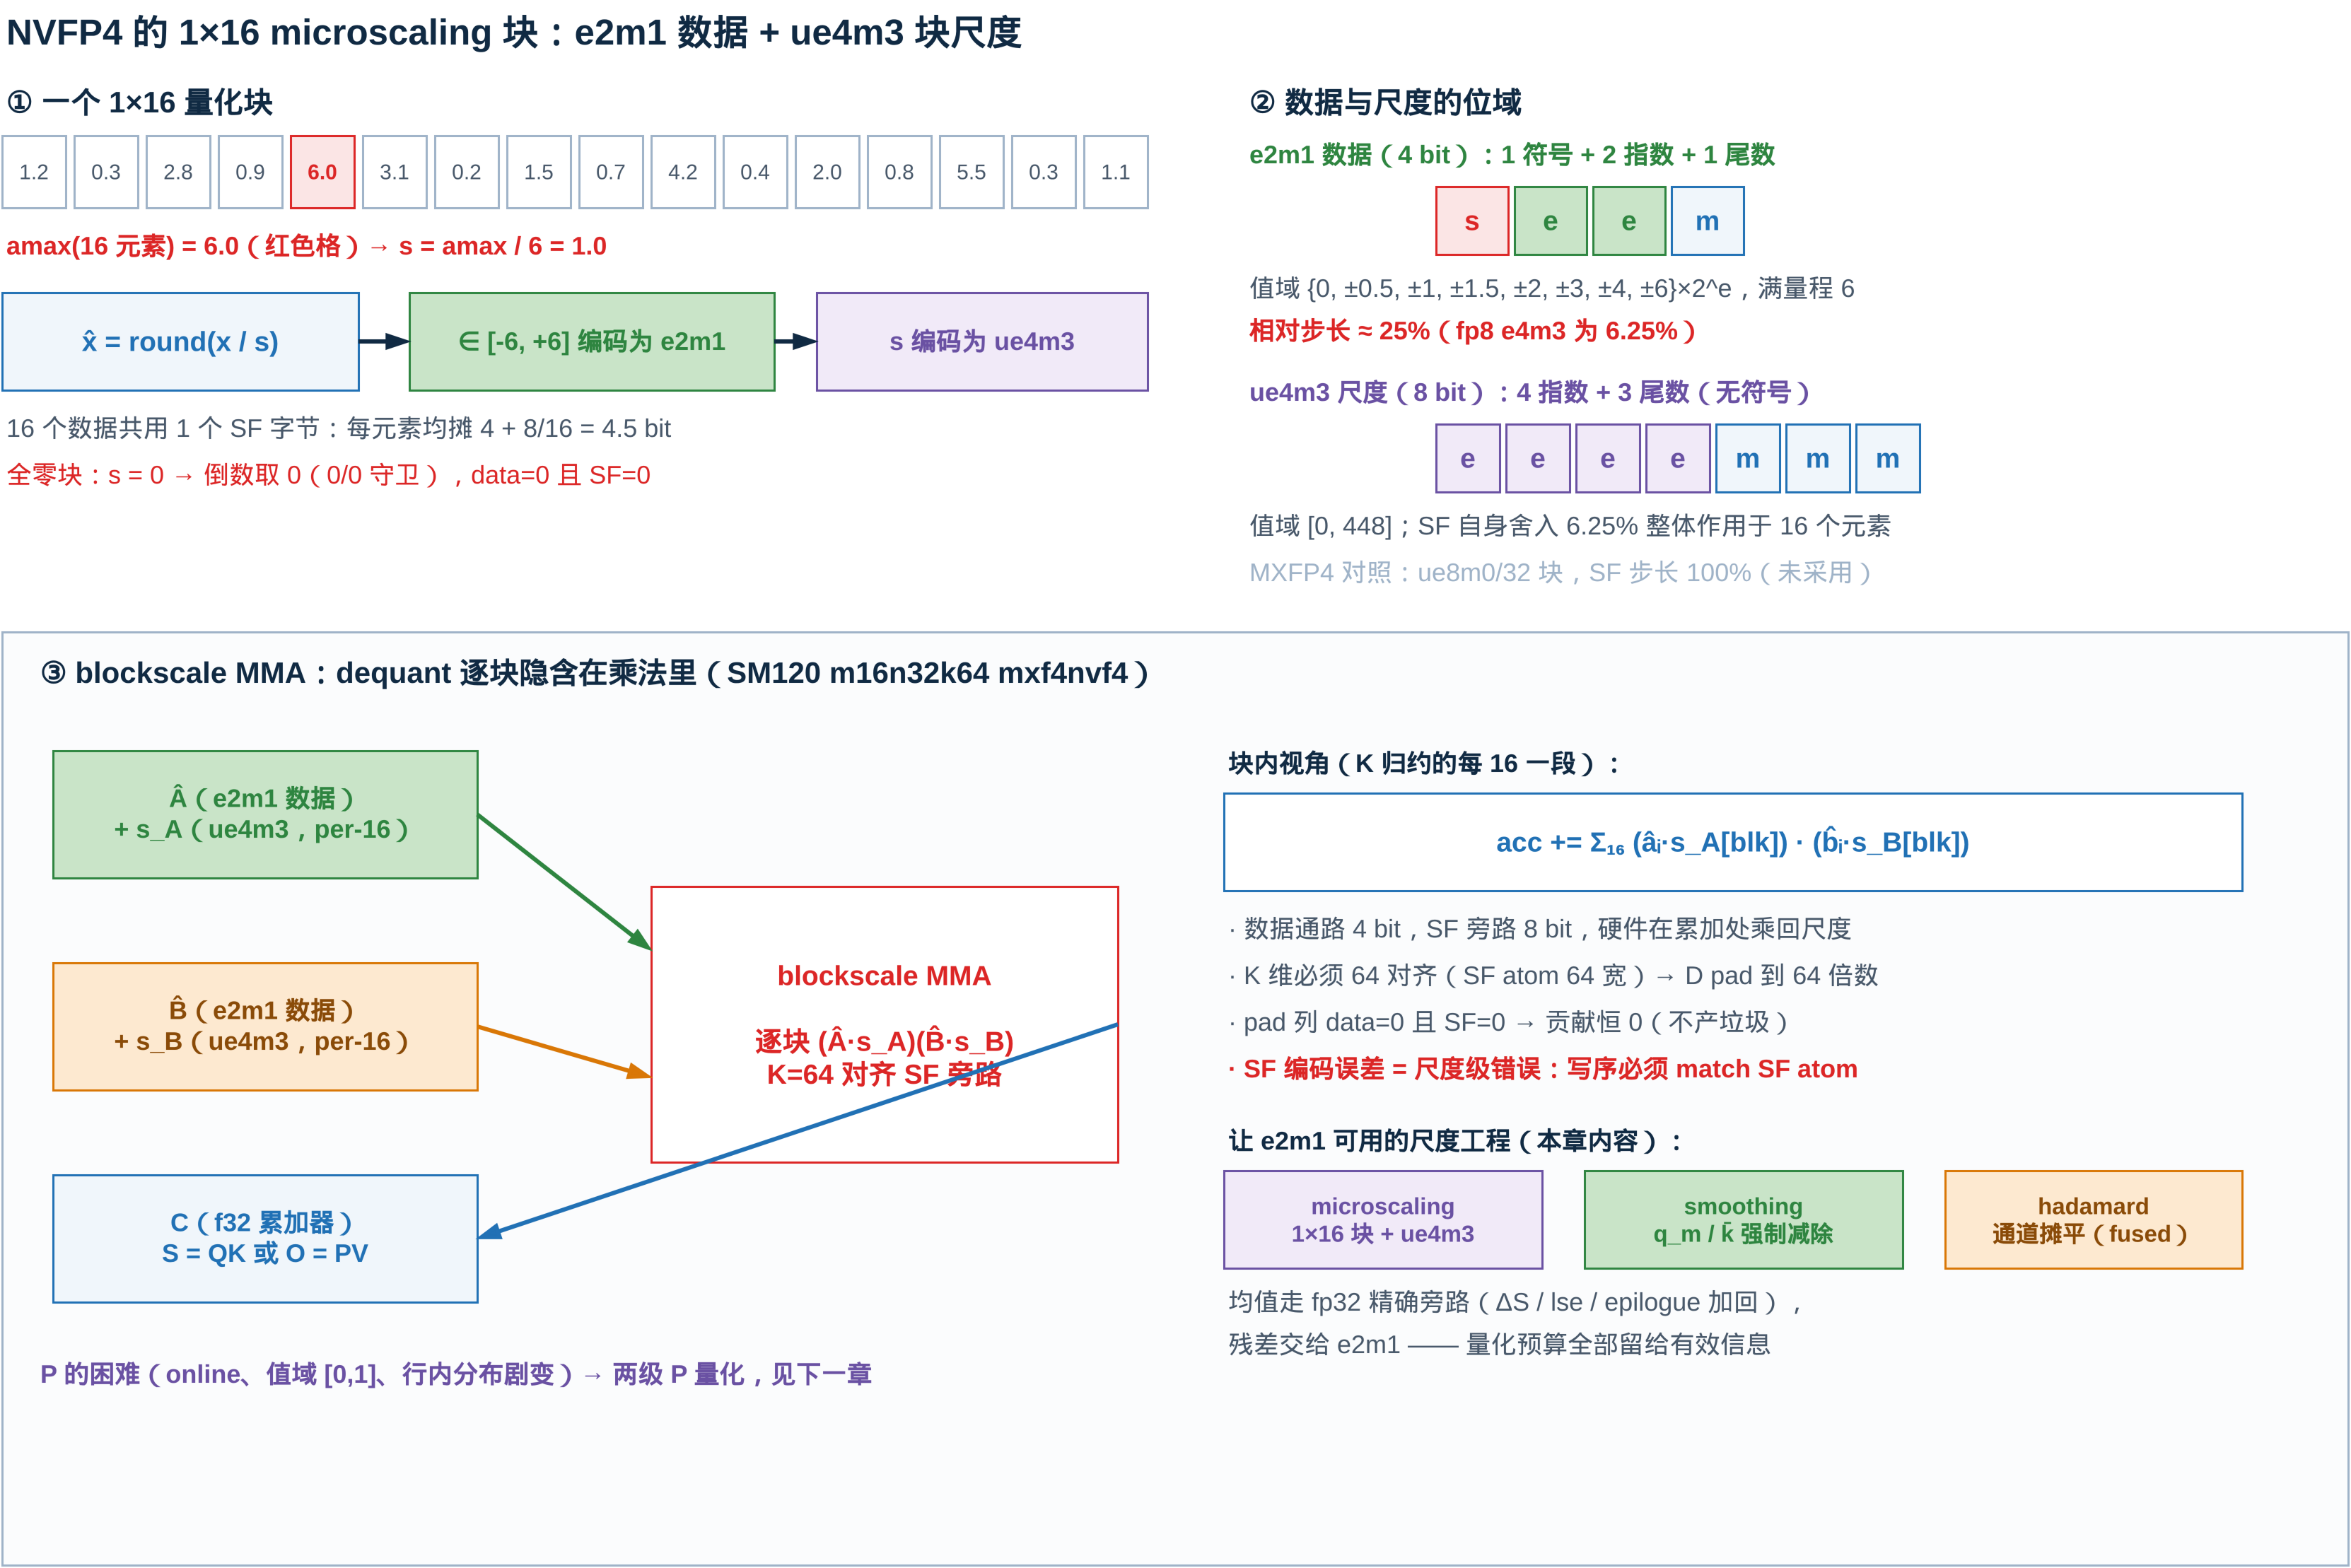
\includegraphics[width=0.98\textwidth]{figures/drawio/fig-31-1-nvfp4-block/fig-31-1-nvfp4-block.png}
  \begin{tikzpicture}
    \node[anchor=west, inner sep=0pt, align=left, font={\fontsize{7.4}{9.3}\selectfont \bfseries }] at (0.37,-0.354) {NVFP4 的 1$\times$16 microscaling 块：e2m1 数据 + ue4m3 块尺度};% w=16.940
    \node[anchor=west, inner sep=0pt, align=left, font={\fontsize{6.1}{7.7}\selectfont \bfseries }] at (0.37,-0.862) {(1) 一个 1$\times$16 量化块};% w=8.316
    \node[draw=gray!55, fill=none, line width=0.5pt, minimum width=0.46cm, minimum height=0.52cm, inner sep=1pt, align=center, text width=0.40cm, font={\fontsize{4.4}{5.5}\selectfont \color{black!65} }] at (0.601,-1.371) {1.2};
    \node[draw=gray!55, fill=none, line width=0.5pt, minimum width=0.46cm, minimum height=0.52cm, inner sep=1pt, align=center, text width=0.40cm, font={\fontsize{4.4}{5.5}\selectfont \color{black!65} }] at (1.124,-1.371) {0.3};
    \node[draw=gray!55, fill=none, line width=0.5pt, minimum width=0.46cm, minimum height=0.52cm, inner sep=1pt, align=center, text width=0.40cm, font={\fontsize{4.4}{5.5}\selectfont \color{black!65} }] at (1.648,-1.371) {2.8};
    \node[draw=gray!55, fill=none, line width=0.5pt, minimum width=0.46cm, minimum height=0.52cm, inner sep=1pt, align=center, text width=0.40cm, font={\fontsize{4.4}{5.5}\selectfont \color{black!65} }] at (2.171,-1.371) {0.9};
    \node[draw=tkRed, fill=tkFillRed, line width=0.5pt, minimum width=0.46cm, minimum height=0.52cm, inner sep=1pt, align=center, text width=0.40cm, font={\fontsize{4.4}{5.5}\selectfont \bfseries \color{tkRed} }] at (2.695,-1.371) {6.0};
    \node[draw=gray!55, fill=none, line width=0.5pt, minimum width=0.46cm, minimum height=0.52cm, inner sep=1pt, align=center, text width=0.40cm, font={\fontsize{4.4}{5.5}\selectfont \color{black!65} }] at (3.219,-1.371) {3.1};
    \node[draw=gray!55, fill=none, line width=0.5pt, minimum width=0.46cm, minimum height=0.52cm, inner sep=1pt, align=center, text width=0.40cm, font={\fontsize{4.4}{5.5}\selectfont \color{black!65} }] at (3.742,-1.371) {0.2};
    \node[draw=gray!55, fill=none, line width=0.5pt, minimum width=0.46cm, minimum height=0.52cm, inner sep=1pt, align=center, text width=0.40cm, font={\fontsize{4.4}{5.5}\selectfont \color{black!65} }] at (4.266,-1.371) {1.5};
    \node[draw=gray!55, fill=none, line width=0.5pt, minimum width=0.46cm, minimum height=0.52cm, inner sep=1pt, align=center, text width=0.40cm, font={\fontsize{4.4}{5.5}\selectfont \color{black!65} }] at (4.789,-1.371) {0.7};
    \node[draw=gray!55, fill=none, line width=0.5pt, minimum width=0.46cm, minimum height=0.52cm, inner sep=1pt, align=center, text width=0.40cm, font={\fontsize{4.4}{5.5}\selectfont \color{black!65} }] at (5.313,-1.371) {4.2};
    \node[draw=gray!55, fill=none, line width=0.5pt, minimum width=0.46cm, minimum height=0.52cm, inner sep=1pt, align=center, text width=0.40cm, font={\fontsize{4.4}{5.5}\selectfont \color{black!65} }] at (5.837,-1.371) {0.4};
    \node[draw=gray!55, fill=none, line width=0.5pt, minimum width=0.46cm, minimum height=0.52cm, inner sep=1pt, align=center, text width=0.40cm, font={\fontsize{4.4}{5.5}\selectfont \color{black!65} }] at (6.36,-1.371) {2.0};
    \node[draw=gray!55, fill=none, line width=0.5pt, minimum width=0.46cm, minimum height=0.52cm, inner sep=1pt, align=center, text width=0.40cm, font={\fontsize{4.4}{5.5}\selectfont \color{black!65} }] at (6.884,-1.371) {0.8};
    \node[draw=gray!55, fill=none, line width=0.5pt, minimum width=0.46cm, minimum height=0.52cm, inner sep=1pt, align=center, text width=0.40cm, font={\fontsize{4.4}{5.5}\selectfont \color{black!65} }] at (7.407,-1.371) {5.5};
    \node[draw=gray!55, fill=none, line width=0.5pt, minimum width=0.46cm, minimum height=0.52cm, inner sep=1pt, align=center, text width=0.40cm, font={\fontsize{4.4}{5.5}\selectfont \color{black!65} }] at (7.931,-1.371) {0.3};
    \node[draw=gray!55, fill=none, line width=0.5pt, minimum width=0.46cm, minimum height=0.52cm, inner sep=1pt, align=center, text width=0.40cm, font={\fontsize{4.4}{5.5}\selectfont \color{black!65} }] at (8.455,-1.371) {1.1};
    \node[anchor=west, inner sep=0pt, align=left, font={\fontsize{5.2}{6.6}\selectfont \bfseries \color{tkRed} }] at (0.37,-1.91) {amax(16 元素) = 6.0（红色格）$\to$ s = amax / 6 = 1.0};% w=8.393
    \node[draw=tkBlue, fill=tkFillBlue, line width=0.5pt, minimum width=2.59cm, minimum height=0.71cm, inner sep=1pt, align=center, text width=2.53cm, font={\fontsize{5.7}{7.1}\selectfont \bfseries \color{tkBlue} }] at (1.663,-2.603) {$\hat{x}$ = round(x / s)};
    \node[draw=tkGreen, fill=tkFillGreen, line width=0.5pt, minimum width=2.65cm, minimum height=0.71cm, inner sep=1pt, align=center, text width=2.59cm, font={\fontsize{5.2}{6.6}\selectfont \bfseries \color{tkGreen!70!black} }] at (4.651,-2.603) {$\in$ [-6, +6] 编码为 e2m1};
    \node[draw=tkPurple, fill=tkFillPurple, line width=0.5pt, minimum width=2.40cm, minimum height=0.71cm, inner sep=1pt, align=center, text width=2.34cm, font={\fontsize{5.2}{6.6}\selectfont \bfseries \color{tkPurple} }] at (7.484,-2.603) {s 编码为 ue4m3};
    \node[anchor=west, inner sep=0pt, align=left, font={\fontsize{5.2}{6.6}\selectfont \color{black!65} }] at (0.37,-3.234) {16 个数据共用 1 个 SF 字节：每元素均摊 4 + 8/16 = 4.5 bit};% w=8.393
    \node[anchor=west, inner sep=0pt, align=left, font={\fontsize{5.2}{6.6}\selectfont \color{tkRed} }] at (0.37,-3.573) {全零块：s = 0 $\to$ 倒数取 0（0/0 守卫），data=0 且 SF=0};% w=8.393
    \node[anchor=west, inner sep=0pt, align=left, font={\fontsize{6.1}{7.7}\selectfont \bfseries }] at (9.394,-0.862) {(2) 数据与尺度的位域};% w=8.008
    \node[anchor=west, inner sep=0pt, align=left, font={\fontsize{5.2}{6.6}\selectfont \bfseries \color{tkGreen!70!black} }] at (9.394,-1.247) {e2m1 数据（4 bit）：1 符号 + 2 指数 + 1 尾数};% w=8.008
    \node[draw=tkRed, fill=tkFillRed, line width=0.5pt, minimum width=0.52cm, minimum height=0.49cm, inner sep=1pt, align=center, text width=0.46cm, font={\fontsize{5.7}{7.1}\selectfont \bfseries \color{tkRed} }] at (11.042,-1.725) {s};
    \node[draw=tkGreen, fill=tkFillGreen, line width=0.5pt, minimum width=0.52cm, minimum height=0.49cm, inner sep=1pt, align=center, text width=0.46cm, font={\fontsize{5.7}{7.1}\selectfont \bfseries \color{tkGreen!70!black} }] at (11.612,-1.725) {e};
    \node[draw=tkGreen, fill=tkFillGreen, line width=0.5pt, minimum width=0.52cm, minimum height=0.49cm, inner sep=1pt, align=center, text width=0.46cm, font={\fontsize{5.7}{7.1}\selectfont \bfseries \color{tkGreen!70!black} }] at (12.181,-1.725) {e};
    \node[draw=tkBlue, fill=tkFillBlue, line width=0.5pt, minimum width=0.52cm, minimum height=0.49cm, inner sep=1pt, align=center, text width=0.46cm, font={\fontsize{5.7}{7.1}\selectfont \bfseries \color{tkBlue} }] at (12.751,-1.725) {m};
    \node[anchor=west, inner sep=0pt, align=left, font={\fontsize{5.2}{6.6}\selectfont \color{black!65} }] at (9.394,-2.218) {值域 {0, $\pm$0.5, $\pm$1, $\pm$1.5, $\pm$2, $\pm$3, $\pm$4, $\pm$6}$\times$2\^{}e，满量程 6};% w=8.008
    \node[anchor=west, inner sep=0pt, align=left, font={\fontsize{5.2}{6.6}\selectfont \bfseries \color{tkRed} }] at (9.394,-2.526) {相对步长 $\approx$ 25\%（fp8 e4m3 为 6.25\%）};% w=8.008
    \node[anchor=west, inner sep=0pt, align=left, font={\fontsize{5.2}{6.6}\selectfont \bfseries \color{tkPurple} }] at (9.394,-2.972) {ue4m3 尺度（8 bit）：4 指数 + 3 尾数（无符号）};% w=8.008
    \node[draw=tkPurple, fill=tkFillPurple, line width=0.5pt, minimum width=0.46cm, minimum height=0.49cm, inner sep=1pt, align=center, text width=0.40cm, font={\fontsize{5.7}{7.1}\selectfont \bfseries \color{tkPurple} }] at (11.011,-3.45) {e};
    \node[draw=tkPurple, fill=tkFillPurple, line width=0.5pt, minimum width=0.46cm, minimum height=0.49cm, inner sep=1pt, align=center, text width=0.40cm, font={\fontsize{5.7}{7.1}\selectfont \bfseries \color{tkPurple} }] at (11.519,-3.45) {e};
    \node[draw=tkPurple, fill=tkFillPurple, line width=0.5pt, minimum width=0.46cm, minimum height=0.49cm, inner sep=1pt, align=center, text width=0.40cm, font={\fontsize{5.7}{7.1}\selectfont \bfseries \color{tkPurple} }] at (12.027,-3.45) {e};
    \node[draw=tkPurple, fill=tkFillPurple, line width=0.5pt, minimum width=0.46cm, minimum height=0.49cm, inner sep=1pt, align=center, text width=0.40cm, font={\fontsize{5.7}{7.1}\selectfont \bfseries \color{tkPurple} }] at (12.536,-3.45) {e};
    \node[draw=tkBlue, fill=tkFillBlue, line width=0.5pt, minimum width=0.46cm, minimum height=0.49cm, inner sep=1pt, align=center, text width=0.40cm, font={\fontsize{5.7}{7.1}\selectfont \bfseries \color{tkBlue} }] at (13.044,-3.45) {m};
    \node[draw=tkBlue, fill=tkFillBlue, line width=0.5pt, minimum width=0.46cm, minimum height=0.49cm, inner sep=1pt, align=center, text width=0.40cm, font={\fontsize{5.7}{7.1}\selectfont \bfseries \color{tkBlue} }] at (13.552,-3.45) {m};
    \node[draw=tkBlue, fill=tkFillBlue, line width=0.5pt, minimum width=0.46cm, minimum height=0.49cm, inner sep=1pt, align=center, text width=0.40cm, font={\fontsize{5.7}{7.1}\selectfont \bfseries \color{tkBlue} }] at (14.06,-3.45) {m};
    \node[anchor=west, inner sep=0pt, align=left, font={\fontsize{5.2}{6.6}\selectfont \color{black!65} }] at (9.394,-3.942) {值域 [0, 448]；SF 自身舍入 6.25\% 整体作用于 16 个元素};% w=8.008
    \node[anchor=west, inner sep=0pt, align=left, font={\fontsize{5.2}{6.6}\selectfont \color{black!45} }] at (9.394,-4.281) {MXFP4 对照：ue8m0/32 块，SF 步长 100\%（未采用）};% w=8.008
    \node[draw=gray!55, fill=black!2, line width=0.5pt, minimum width=17.03cm, minimum height=6.78cm, inner sep=1pt, align=center, text width=16.97cm, font={\fontsize{5.7}{7.1}\selectfont }] at (8.886,-8.1) {};
    \node[anchor=west, inner sep=0pt, align=left, font={\fontsize{6.1}{7.7}\selectfont \bfseries }] at (0.616,-5.005) {(3) blockscale MMA：dequant 逐块隐含在乘法里（SM120 m16n32k64 mxf4nvf4）};% w=16.478
    \node[draw=tkGreen, fill=tkFillGreen, line width=0.5pt, minimum width=3.08cm, minimum height=0.92cm, inner sep=1pt, align=center, text width=3.02cm, font={\fontsize{5.2}{6.6}\selectfont \bfseries \color{tkGreen!70!black} }] at (2.279,-6.037) {$\hat{A}$（e2m1 数据）\\+ s\_A（ue4m3，per-16）};
    \node[draw=tkOrange, fill=tkFillOrange, line width=0.5pt, minimum width=3.08cm, minimum height=0.92cm, inner sep=1pt, align=center, text width=3.02cm, font={\fontsize{5.2}{6.6}\selectfont \bfseries \color{tkOrange!75!black} }] at (2.279,-7.577) {$\hat{B}$（e2m1 数据）\\+ s\_B（ue4m3，per-16）};
    \node[draw=tkBlue, fill=tkFillBlue, line width=0.5pt, minimum width=3.08cm, minimum height=0.92cm, inner sep=1pt, align=center, text width=3.02cm, font={\fontsize{5.2}{6.6}\selectfont \bfseries \color{tkBlue} }] at (2.279,-9.117) {C（f32 累加器）\\S = QK 或 O = PV};
    \node[draw=tkRed, fill=none, line width=0.5pt, minimum width=3.39cm, minimum height=2.00cm, inner sep=1pt, align=center, text width=3.33cm, font={\fontsize{5.7}{7.1}\selectfont \bfseries \color{tkRed} }] at (6.776,-7.561) {blockscale MMA\\逐块 ($\hat{A}$$\cdot$s\_A)($\hat{B}$$\cdot$s\_B)\\K=64 对齐 SF 旁路};
    \node[anchor=west, inner sep=0pt, align=left, font={\fontsize{5.2}{6.6}\selectfont \bfseries }] at (9.24,-5.667) {块内视角（K 归约的每 16 一段）：};% w=7.700
    \node[draw=tkBlue, fill=none, line width=0.5pt, minimum width=7.39cm, minimum height=0.71cm, inner sep=1pt, align=center, text width=7.33cm, font={\fontsize{5.7}{7.1}\selectfont \bfseries \color{tkBlue} }] at (12.936,-6.237) {acc += $\Sigma$$_1$$_6$ ($\hat{a}$$_i$$\cdot$s\_A[blk]) $\cdot$ ($\hat{b}$$_i$$\cdot$s\_B[blk])};
    \node[anchor=west, inner sep=0pt, align=left, font={\fontsize{5.2}{6.6}\selectfont \color{black!65} }] at (9.24,-6.868) {$\cdot$ 数据通路 4 bit，SF 旁路 8 bit，硬件在累加处乘回尺度};% w=7.700
    \node[anchor=west, inner sep=0pt, align=left, font={\fontsize{5.2}{6.6}\selectfont \color{black!65} }] at (9.24,-7.207) {$\cdot$ K 维必须 64 对齐（SF atom 64 宽）$\to$ D pad 到 64 倍数};% w=7.700
    \node[anchor=west, inner sep=0pt, align=left, font={\fontsize{5.2}{6.6}\selectfont \color{black!65} }] at (9.24,-7.546) {$\cdot$ pad 列 data=0 且 SF=0 $\to$ 贡献恒 0（不产垃圾）};% w=7.700
    \node[anchor=west, inner sep=0pt, align=left, font={\fontsize{5.2}{6.6}\selectfont \bfseries \color{tkRed} }] at (9.24,-7.885) {$\cdot$ SF 编码误差 = 尺度级错误：写序必须 match SF atom};% w=7.700
    \node[anchor=west, inner sep=0pt, align=left, font={\fontsize{5.2}{6.6}\selectfont \bfseries }] at (9.24,-8.408) {让 e2m1 可用的尺度工程（本章内容）：};% w=7.700
    \node[draw=tkPurple, fill=tkFillPurple, line width=0.5pt, minimum width=2.31cm, minimum height=0.71cm, inner sep=1pt, align=center, text width=2.25cm, font={\fontsize{4.8}{6.0}\selectfont \bfseries \color{tkPurple} }] at (10.395,-8.978) {microscaling\\1$\times$16 块 + ue4m3};
    \node[draw=tkGreen, fill=tkFillGreen, line width=0.5pt, minimum width=2.31cm, minimum height=0.71cm, inner sep=1pt, align=center, text width=2.25cm, font={\fontsize{4.8}{6.0}\selectfont \bfseries \color{tkGreen!70!black} }] at (13.013,-8.978) {smoothing\\q\_m / $\bar{k}$ 强制减除};
    \node[draw=tkOrange, fill=tkFillOrange, line width=0.5pt, minimum width=2.16cm, minimum height=0.71cm, inner sep=1pt, align=center, text width=2.09cm, font={\fontsize{4.8}{6.0}\selectfont \bfseries \color{tkOrange!75!black} }] at (15.554,-8.978) {hadamard\\通道摊平（fused）};
    \node[anchor=west, inner sep=0pt, align=left, font={\fontsize{5.2}{6.6}\selectfont \color{black!65} }] at (9.24,-9.579) {均值走 fp32 精确旁路（$\Delta$S / lse / epilogue 加回），};% w=7.700
    \node[anchor=west, inner sep=0pt, align=left, font={\fontsize{5.2}{6.6}\selectfont \color{black!65} }] at (9.24,-9.887) {残差交给 e2m1 ------ 量化预算全部留给有效信息};% w=7.700
    \node[anchor=west, inner sep=0pt, align=left, font={\fontsize{5.2}{6.6}\selectfont \bfseries \color{tkPurple} }] at (0.616,-10.102) {P 的困难（online、值域 [0,1]、行内分布剧变）$\to$ 两级 P 量化，见下一章};% w=8.316
    \draw[black!75, line width=0.8pt, -{Stealth[length=2.2pt,width=1.8pt]}] (2.957,-2.603) -- (3.326,-2.603);
    \draw[black!75, line width=0.8pt, -{Stealth[length=2.2pt,width=1.8pt]}] (5.975,-2.603) -- (6.283,-2.603);
    \draw[tkGreen, line width=0.8pt, -{Stealth[length=2.2pt,width=1.8pt]}] (3.819,-6.037) -- (5.082,-7.022);
    \draw[tkOrange, line width=0.8pt, -{Stealth[length=2.2pt,width=1.8pt]}] (3.819,-7.577) -- (5.082,-7.946);
    \draw[tkBlue, line width=0.8pt, -{Stealth[length=2.2pt,width=1.8pt]}] (8.47,-7.561) -- (3.819,-9.117);
  \end{tikzpicture}
  \caption{NVFP4 的 $1\times16$ microscaling 块：e2m1 数据位域与
  ue4m3 块尺度。$s_{block}=\mathrm{amax}/6$ 除进数据、乘回在
  blockscale MMA 内逐块完成。}
  \label{fig:31-1}
\end{figure}

\begin{figure}[htbp]
  \centering
  % was: 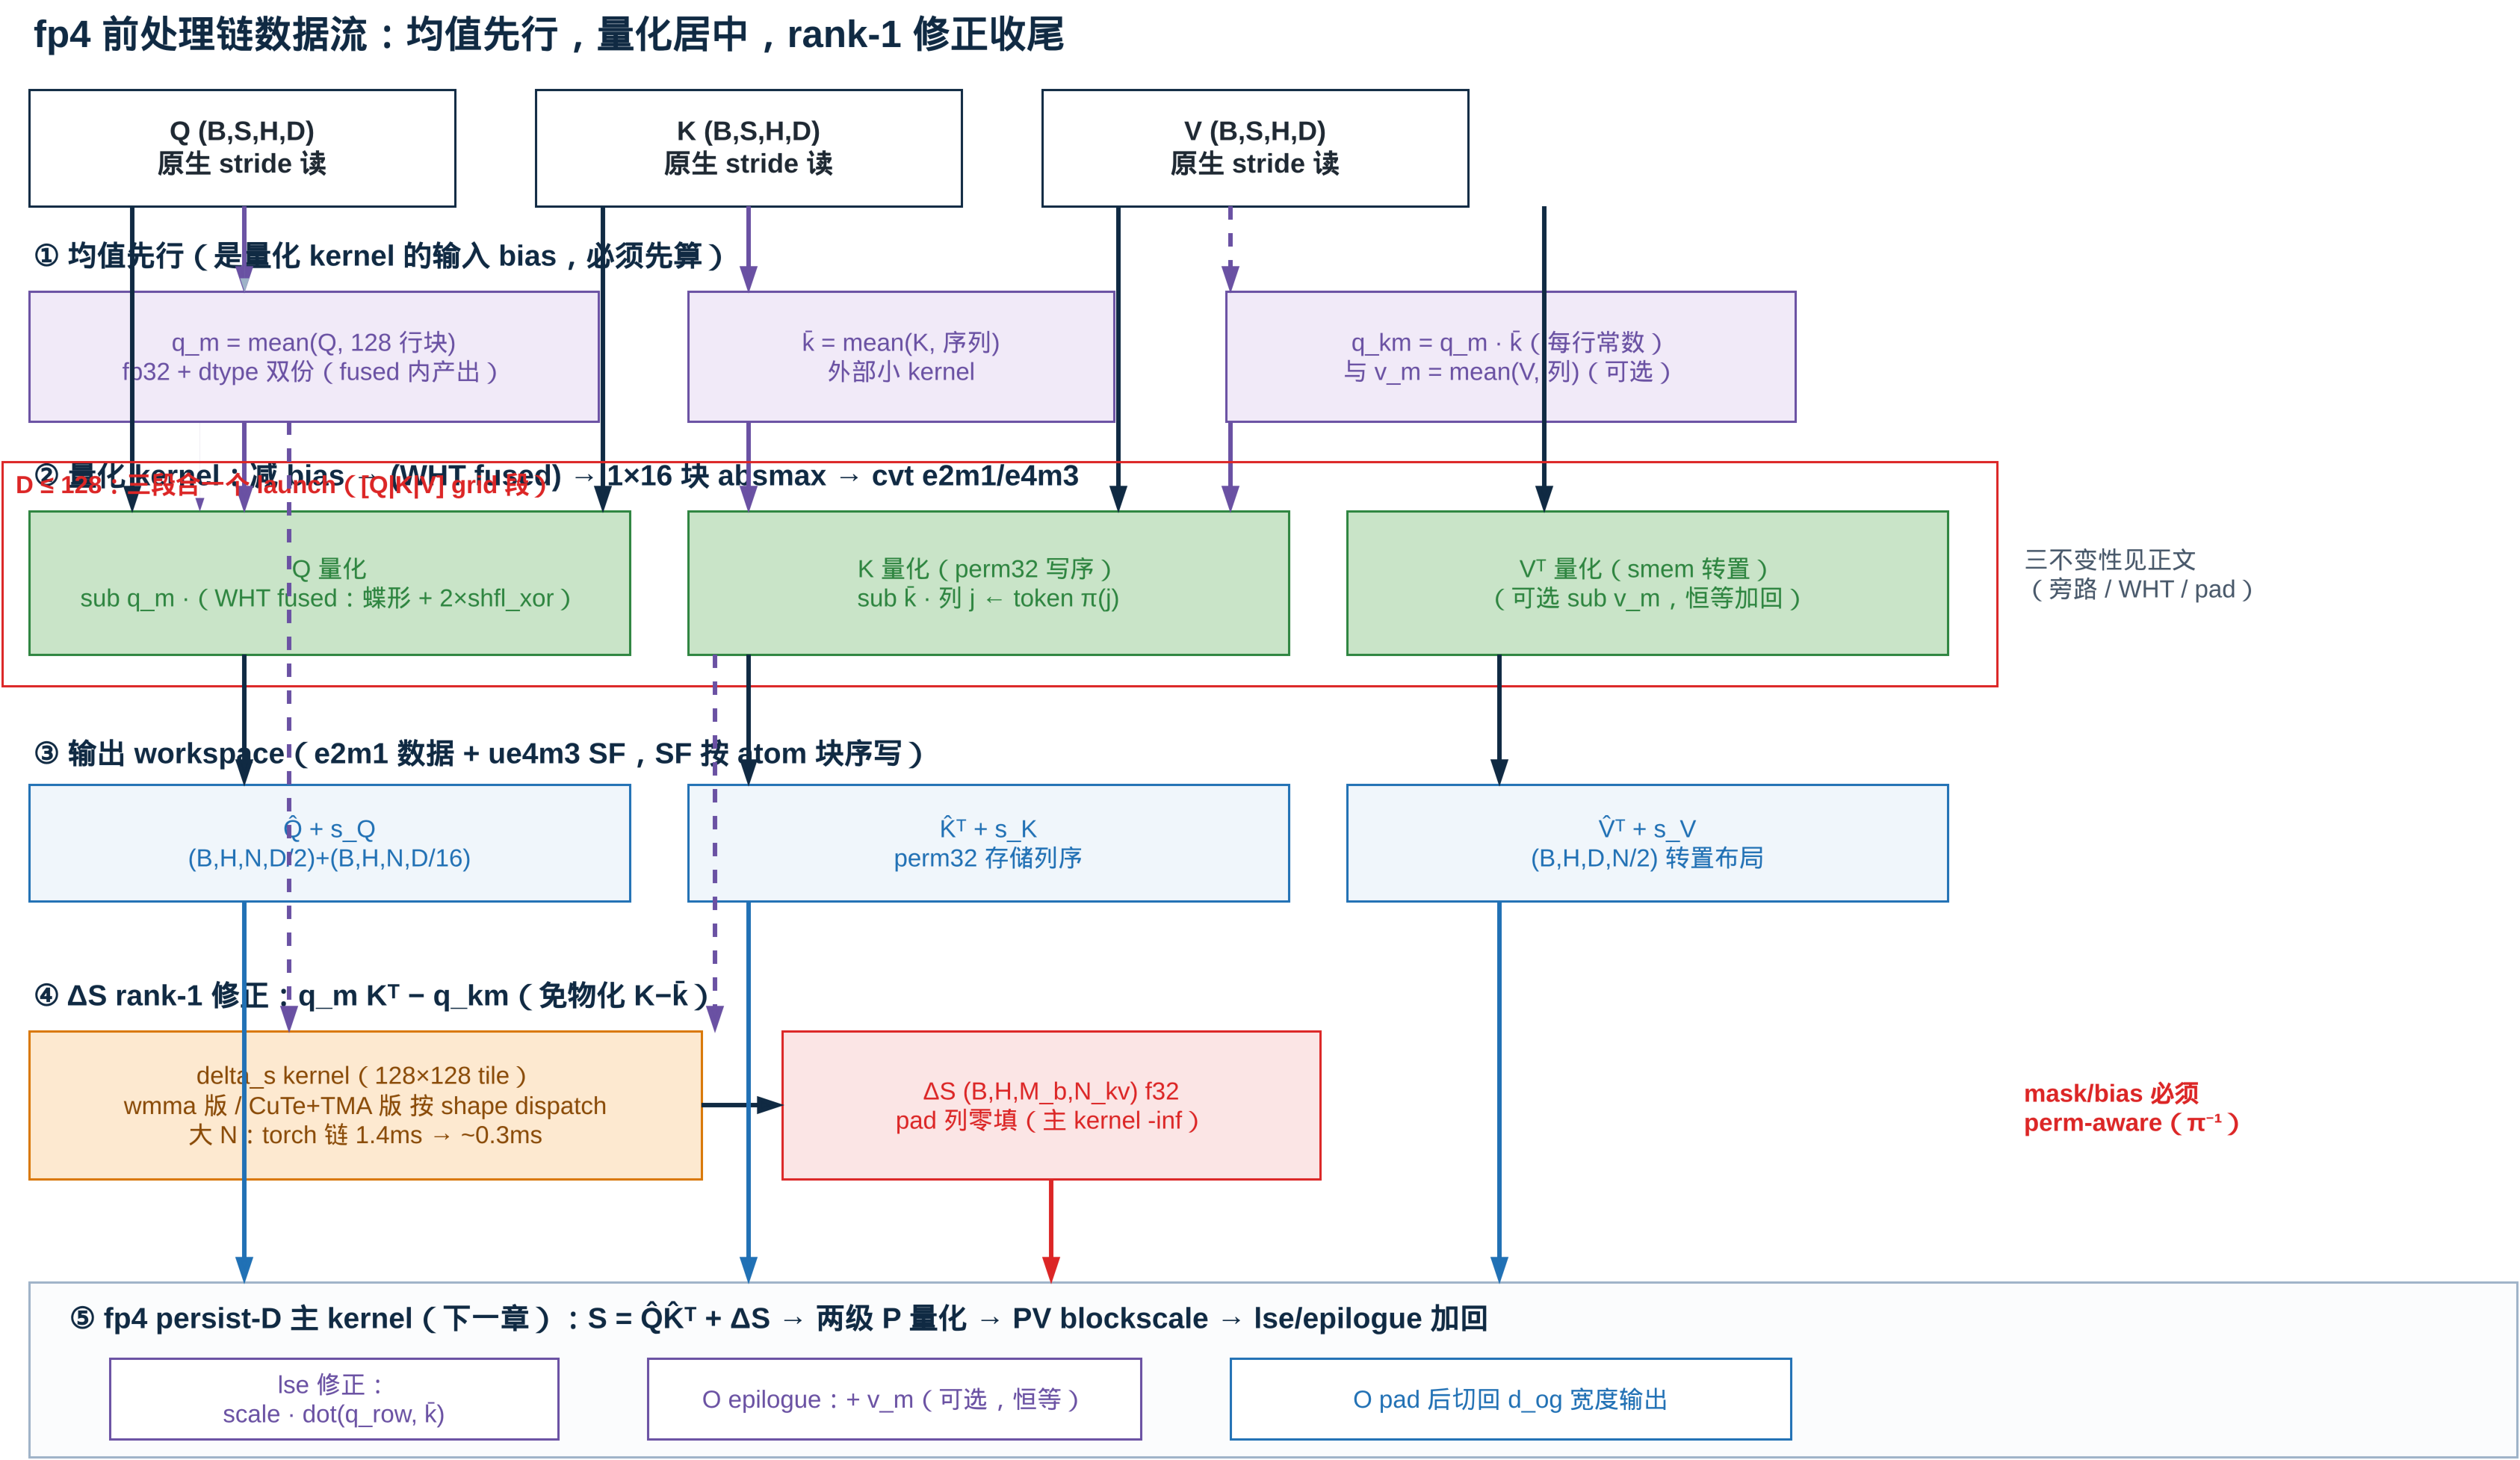
\includegraphics[width=0.98\textwidth]{figures/drawio/fig-31-2-fp4-pipeline/fig-31-2-fp4-pipeline.png}
  \begin{tikzpicture}
    \node[anchor=west, inner sep=0pt, align=left, font={\fontsize{7.4}{9.3}\selectfont \bfseries }] at (0.37,-0.354) {fp4 前处理链数据流：均值先行，量化居中，rank-1 修正收尾};% w=17.094
    \node[draw=black!75, fill=none, line width=0.5pt, minimum width=2.93cm, minimum height=0.80cm, inner sep=1pt, align=center, text width=2.86cm, font={\fontsize{5.2}{6.6}\selectfont \bfseries }] at (1.833,-1.14) {Q (B,S,H,D)\\原生 stride 读};
    \node[draw=black!75, fill=none, line width=0.5pt, minimum width=2.93cm, minimum height=0.80cm, inner sep=1pt, align=center, text width=2.86cm, font={\fontsize{5.2}{6.6}\selectfont \bfseries }] at (5.313,-1.14) {K (B,S,H,D)\\原生 stride 读};
    \node[draw=black!75, fill=none, line width=0.5pt, minimum width=2.93cm, minimum height=0.80cm, inner sep=1pt, align=center, text width=2.86cm, font={\fontsize{5.2}{6.6}\selectfont \bfseries }] at (8.793,-1.14) {V (B,S,H,D)\\原生 stride 读};
    \node[anchor=west, inner sep=0pt, align=left, font={\fontsize{5.7}{7.1}\selectfont \bfseries }] at (0.37,-1.879) {(1) 均值先行（是量化 kernel 的输入 bias，必须先算）};% w=17.094
    \node[draw=tkPurple, fill=tkFillPurple, line width=0.5pt, minimum width=3.91cm, minimum height=0.89cm, inner sep=1pt, align=center, text width=3.85cm, font={\fontsize{4.8}{6.0}\selectfont \color{tkPurple} }] at (2.325,-2.572) {q\_m = mean(Q, 128 行块)\\fp32 + dtype 双份（fused 内产出）};
    \node[draw=tkPurple, fill=tkFillPurple, line width=0.5pt, minimum width=2.93cm, minimum height=0.89cm, inner sep=1pt, align=center, text width=2.86cm, font={\fontsize{4.8}{6.0}\selectfont \color{tkPurple} }] at (6.36,-2.572) {$\bar{k}$ = mean(K, 序列)\\外部小 kernel};
    \node[draw=tkPurple, fill=tkFillPurple, line width=0.5pt, minimum width=3.91cm, minimum height=0.89cm, inner sep=1pt, align=center, text width=3.85cm, font={\fontsize{4.8}{6.0}\selectfont \color{tkPurple} }] at (10.549,-2.572) {q\_km = q\_m $\cdot$ $\bar{k}$（每行常数）\\与 v\_m = mean(V, 列)（可选）};
    \node[anchor=west, inner sep=0pt, align=left, font={\fontsize{5.7}{7.1}\selectfont \bfseries }] at (0.37,-3.388) {(2) 量化 kernel：减 bias $\to$ (WHT fused) $\to$ 1$\times$16 块 absmax $\to$ cvt e2m1/e4m3};% w=17.094
    \node[draw=tkGreen, fill=tkFillGreen, line width=0.5pt, minimum width=4.13cm, minimum height=0.99cm, inner sep=1pt, align=center, text width=4.07cm, font={\fontsize{4.8}{6.0}\selectfont \color{tkGreen!70!black} }] at (2.433,-4.127) {Q 量化\\sub q\_m $\cdot$（WHT fused：蝶形 + 2$\times$shfl\_xor）};
    \node[draw=tkGreen, fill=tkFillGreen, line width=0.5pt, minimum width=4.13cm, minimum height=0.99cm, inner sep=1pt, align=center, text width=4.07cm, font={\fontsize{4.8}{6.0}\selectfont \color{tkGreen!70!black} }] at (6.961,-4.127) {K 量化（perm32 写序）\\sub $\bar{k}$ $\cdot$ 列 j $\leftarrow$ token $\pi$(j)};
    \node[draw=tkGreen, fill=tkFillGreen, line width=0.5pt, minimum width=4.13cm, minimum height=0.99cm, inner sep=1pt, align=center, text width=4.07cm, font={\fontsize{4.8}{6.0}\selectfont \color{tkGreen!70!black} }] at (11.488,-4.127) {V$^{\top}$ 量化（smem 转置）\\（可选 sub v\_m，恒等加回）};
    \node[draw=tkRed, fill=none, line width=0.5pt, minimum width=13.71cm, minimum height=1.54cm, inner sep=1pt, align=center, text width=13.64cm, font={\fontsize{5.7}{7.1}\selectfont }] at (7.038,-4.066) {};
    \node[anchor=west, inner sep=0pt, align=left, font={\fontsize{4.8}{6.0}\selectfont \bfseries \color{tkRed} }] at (0.246,-3.049) {D $\leq$ 128：三段合一个 launch（[Q|K|V] grid 段）};% w=6.160
    \node[anchor=west, inner sep=0pt, align=left, font={\fontsize{5.7}{7.1}\selectfont \bfseries }] at (0.37,-5.298) {(3) 输出 workspace（e2m1 数据 + ue4m3 SF，SF 按 atom 块序写）};% w=17.094
    \node[draw=tkBlue, fill=tkFillBlue, line width=0.5pt, minimum width=4.13cm, minimum height=0.80cm, inner sep=1pt, align=center, text width=4.07cm, font={\fontsize{4.8}{6.0}\selectfont \color{tkBlue} }] at (2.433,-5.914) {$\hat{Q}$ + s\_Q\\(B,H,N,D/2)+(B,H,N,D/16)};
    \node[draw=tkBlue, fill=tkFillBlue, line width=0.5pt, minimum width=4.13cm, minimum height=0.80cm, inner sep=1pt, align=center, text width=4.07cm, font={\fontsize{4.8}{6.0}\selectfont \color{tkBlue} }] at (6.961,-5.914) {$\hat{K}$$^{\top}$ + s\_K\\perm32 存储列序};
    \node[draw=tkBlue, fill=tkFillBlue, line width=0.5pt, minimum width=4.13cm, minimum height=0.80cm, inner sep=1pt, align=center, text width=4.07cm, font={\fontsize{4.8}{6.0}\selectfont \color{tkBlue} }] at (11.488,-5.914) {$\hat{V}$$^{\top}$ + s\_V\\(B,H,D,N/2) 转置布局};
    \node[anchor=west, inner sep=0pt, align=left, font={\fontsize{5.7}{7.1}\selectfont \bfseries }] at (0.37,-6.961) {(4) $\Delta$S rank-1 修正：q\_m K$^{\top}$ $-$ q\_km（免物化 K$-$$\bar{k}$）};% w=17.094
    \node[draw=tkOrange, fill=tkFillOrange, line width=0.5pt, minimum width=4.62cm, minimum height=1.02cm, inner sep=1pt, align=center, text width=4.56cm, font={\fontsize{4.8}{6.0}\selectfont \color{tkOrange!75!black} }] at (2.68,-7.715) {delta\_s kernel（128$\times$128 tile）\\wmma 版 / CuTe+TMA 版 按 shape dispatch\\大 N：torch 链 1.4ms $\to$ \textasciitilde{}0.3ms};
    \node[draw=tkRed, fill=tkFillRed, line width=0.5pt, minimum width=3.70cm, minimum height=1.02cm, inner sep=1pt, align=center, text width=3.63cm, font={\fontsize{4.8}{6.0}\selectfont \color{tkRed} }] at (7.392,-7.715) {$\Delta$S (B,H,M\_b,N\_kv) f32\\pad 列零填（主 kernel -inf）};
    \node[draw=gray!55, fill=black!2, line width=0.5pt, minimum width=17.09cm, minimum height=1.20cm, inner sep=1pt, align=center, text width=17.03cm, font={\fontsize{5.7}{7.1}\selectfont }] at (8.917,-9.533) {};
    \node[anchor=west, inner sep=0pt, align=left, font={\fontsize{5.7}{7.1}\selectfont \bfseries }] at (0.616,-9.178) {(5) fp4 persist-D 主 kernel（下一章）：S = $\hat{Q}$$\hat{K}$$^{\top}$ + $\Delta$S $\to$ 两级 P 量化 $\to$ PV blockscale $\to$ lse/epilogue 加回};% w=16.478
    \node[draw=tkPurple, fill=none, line width=0.5pt, minimum width=3.08cm, minimum height=0.55cm, inner sep=1pt, align=center, text width=3.02cm, font={\fontsize{4.8}{6.0}\selectfont \color{tkPurple} }] at (2.464,-9.733) {lse 修正：\\scale $\cdot$ dot(q\_row, $\bar{k}$)};
    \node[draw=tkPurple, fill=none, line width=0.5pt, minimum width=3.39cm, minimum height=0.55cm, inner sep=1pt, align=center, text width=3.33cm, font={\fontsize{4.8}{6.0}\selectfont \color{tkPurple} }] at (6.314,-9.733) {O epilogue：+ v\_m（可选，恒等）};
    \node[draw=tkBlue, fill=none, line width=0.5pt, minimum width=3.85cm, minimum height=0.55cm, inner sep=1pt, align=center, text width=3.79cm, font={\fontsize{4.8}{6.0}\selectfont \color{tkBlue} }] at (10.549,-9.733) {O pad 后切回 d\_og 宽度输出};
    \node[anchor=west, inner sep=0pt, align=left, font={\fontsize{4.8}{6.0}\selectfont \color{black!65} }] at (14.045,-4.066) {三不变性见正文\\（旁路 / WHT / pad）};% w=3.388
    \node[anchor=west, inner sep=0pt, align=left, font={\fontsize{4.8}{6.0}\selectfont \bfseries \color{tkRed} }] at (14.045,-7.731) {mask/bias 必须\\perm-aware（$\pi$$^{-1}$）};% w=3.388
    \draw[tkPurple, line width=0.8pt, -{Stealth[length=2.2pt,width=1.8pt]}] (1.848,-1.54) -- (1.848,-2.125);
    \draw[tkPurple, line width=0.8pt, -{Stealth[length=2.2pt,width=1.8pt]}] (5.313,-1.54) -- (5.313,-2.125);
    \draw[tkPurple, line width=0.8pt, dashed, -{Stealth[length=2.2pt,width=1.8pt]}] (8.624,-1.54) -- (8.624,-2.125);
    \draw[tkPurple, line width=0.8pt, -{Stealth[length=2.2pt,width=1.8pt]}] (1.848,-3.018) -- (1.848,-3.634);
    \draw[tkPurple, line width=0.8pt, -{Stealth[length=2.2pt,width=1.8pt]}] (5.313,-3.018) -- (5.313,-3.634);
    \draw[tkPurple, line width=0.8pt, -{Stealth[length=2.2pt,width=1.8pt]}] (8.624,-3.018) -- (8.624,-3.634);
    \draw[gray!55, line width=0.5pt, -{Stealth[length=2.2pt,width=1.8pt]}] (1.848,-1.54) -- (1.848,-2.125);
    \draw[black!75, line width=0.8pt, -{Stealth[length=2.2pt,width=1.8pt]}] (1.078,-1.54) -- (1.078,-3.634);
    \draw[black!75, line width=0.8pt, -{Stealth[length=2.2pt,width=1.8pt]}] (4.312,-1.54) -- (4.312,-3.634);
    \draw[black!75, line width=0.8pt, -{Stealth[length=2.2pt,width=1.8pt]}] (7.854,-1.54) -- (7.854,-3.634);
    \draw[black!75, line width=0.8pt, -{Stealth[length=2.2pt,width=1.8pt]}] (10.78,-1.54) -- (10.78,-3.634);
    \draw[black!75, line width=0.8pt, -{Stealth[length=2.2pt,width=1.8pt]}] (1.848,-4.62) -- (1.848,-5.513);
    \draw[black!75, line width=0.8pt, -{Stealth[length=2.2pt,width=1.8pt]}] (5.313,-4.62) -- (5.313,-5.513);
    \draw[black!75, line width=0.8pt, -{Stealth[length=2.2pt,width=1.8pt]}] (10.472,-4.62) -- (10.472,-5.513);
    \draw[black!75, line width=0.8pt, -{Stealth[length=2.2pt,width=1.8pt]}] (4.99,-7.715) -- (5.544,-7.715);
    \draw[tkPurple, line width=0.5pt, -{Stealth[length=2.2pt,width=1.8pt]}] (1.54,-3.018) -- (1.54,-3.634);
    \draw[tkPurple, line width=0.8pt, dashed, -{Stealth[length=2.2pt,width=1.8pt]}] (2.156,-3.018) -- (2.156,-4.558) -- (2.156,-7.207);
    \draw[tkPurple, line width=0.8pt, dashed, -{Stealth[length=2.2pt,width=1.8pt]}] (5.082,-4.62) -- (5.082,-6.314) -- (5.082,-7.207);
    \draw[tkBlue, line width=0.8pt, -{Stealth[length=2.2pt,width=1.8pt]}] (1.848,-6.314) -- (1.848,-8.932);
    \draw[tkBlue, line width=0.8pt, -{Stealth[length=2.2pt,width=1.8pt]}] (5.313,-6.314) -- (5.313,-8.932);
    \draw[tkBlue, line width=0.8pt, -{Stealth[length=2.2pt,width=1.8pt]}] (10.472,-6.314) -- (10.472,-8.932);
    \draw[tkRed, line width=0.8pt, -{Stealth[length=2.2pt,width=1.8pt]}] (7.392,-8.224) -- (7.392,-8.932);
  \end{tikzpicture}
  \caption{fp4 前处理链数据流（$D\le128$ 走 fused 单 launch 路径）：
  $\bar k$/$q_m$ 均值先行的原因是它们是量化 kernel 的输入 bias；
  hadamard 下 $q_m^{rot}$ 在 fused kernel 内顺带产出。}
  \label{fig:31-2}
\end{figure}

\begin{figure}[htbp]
  \centering
  % was: 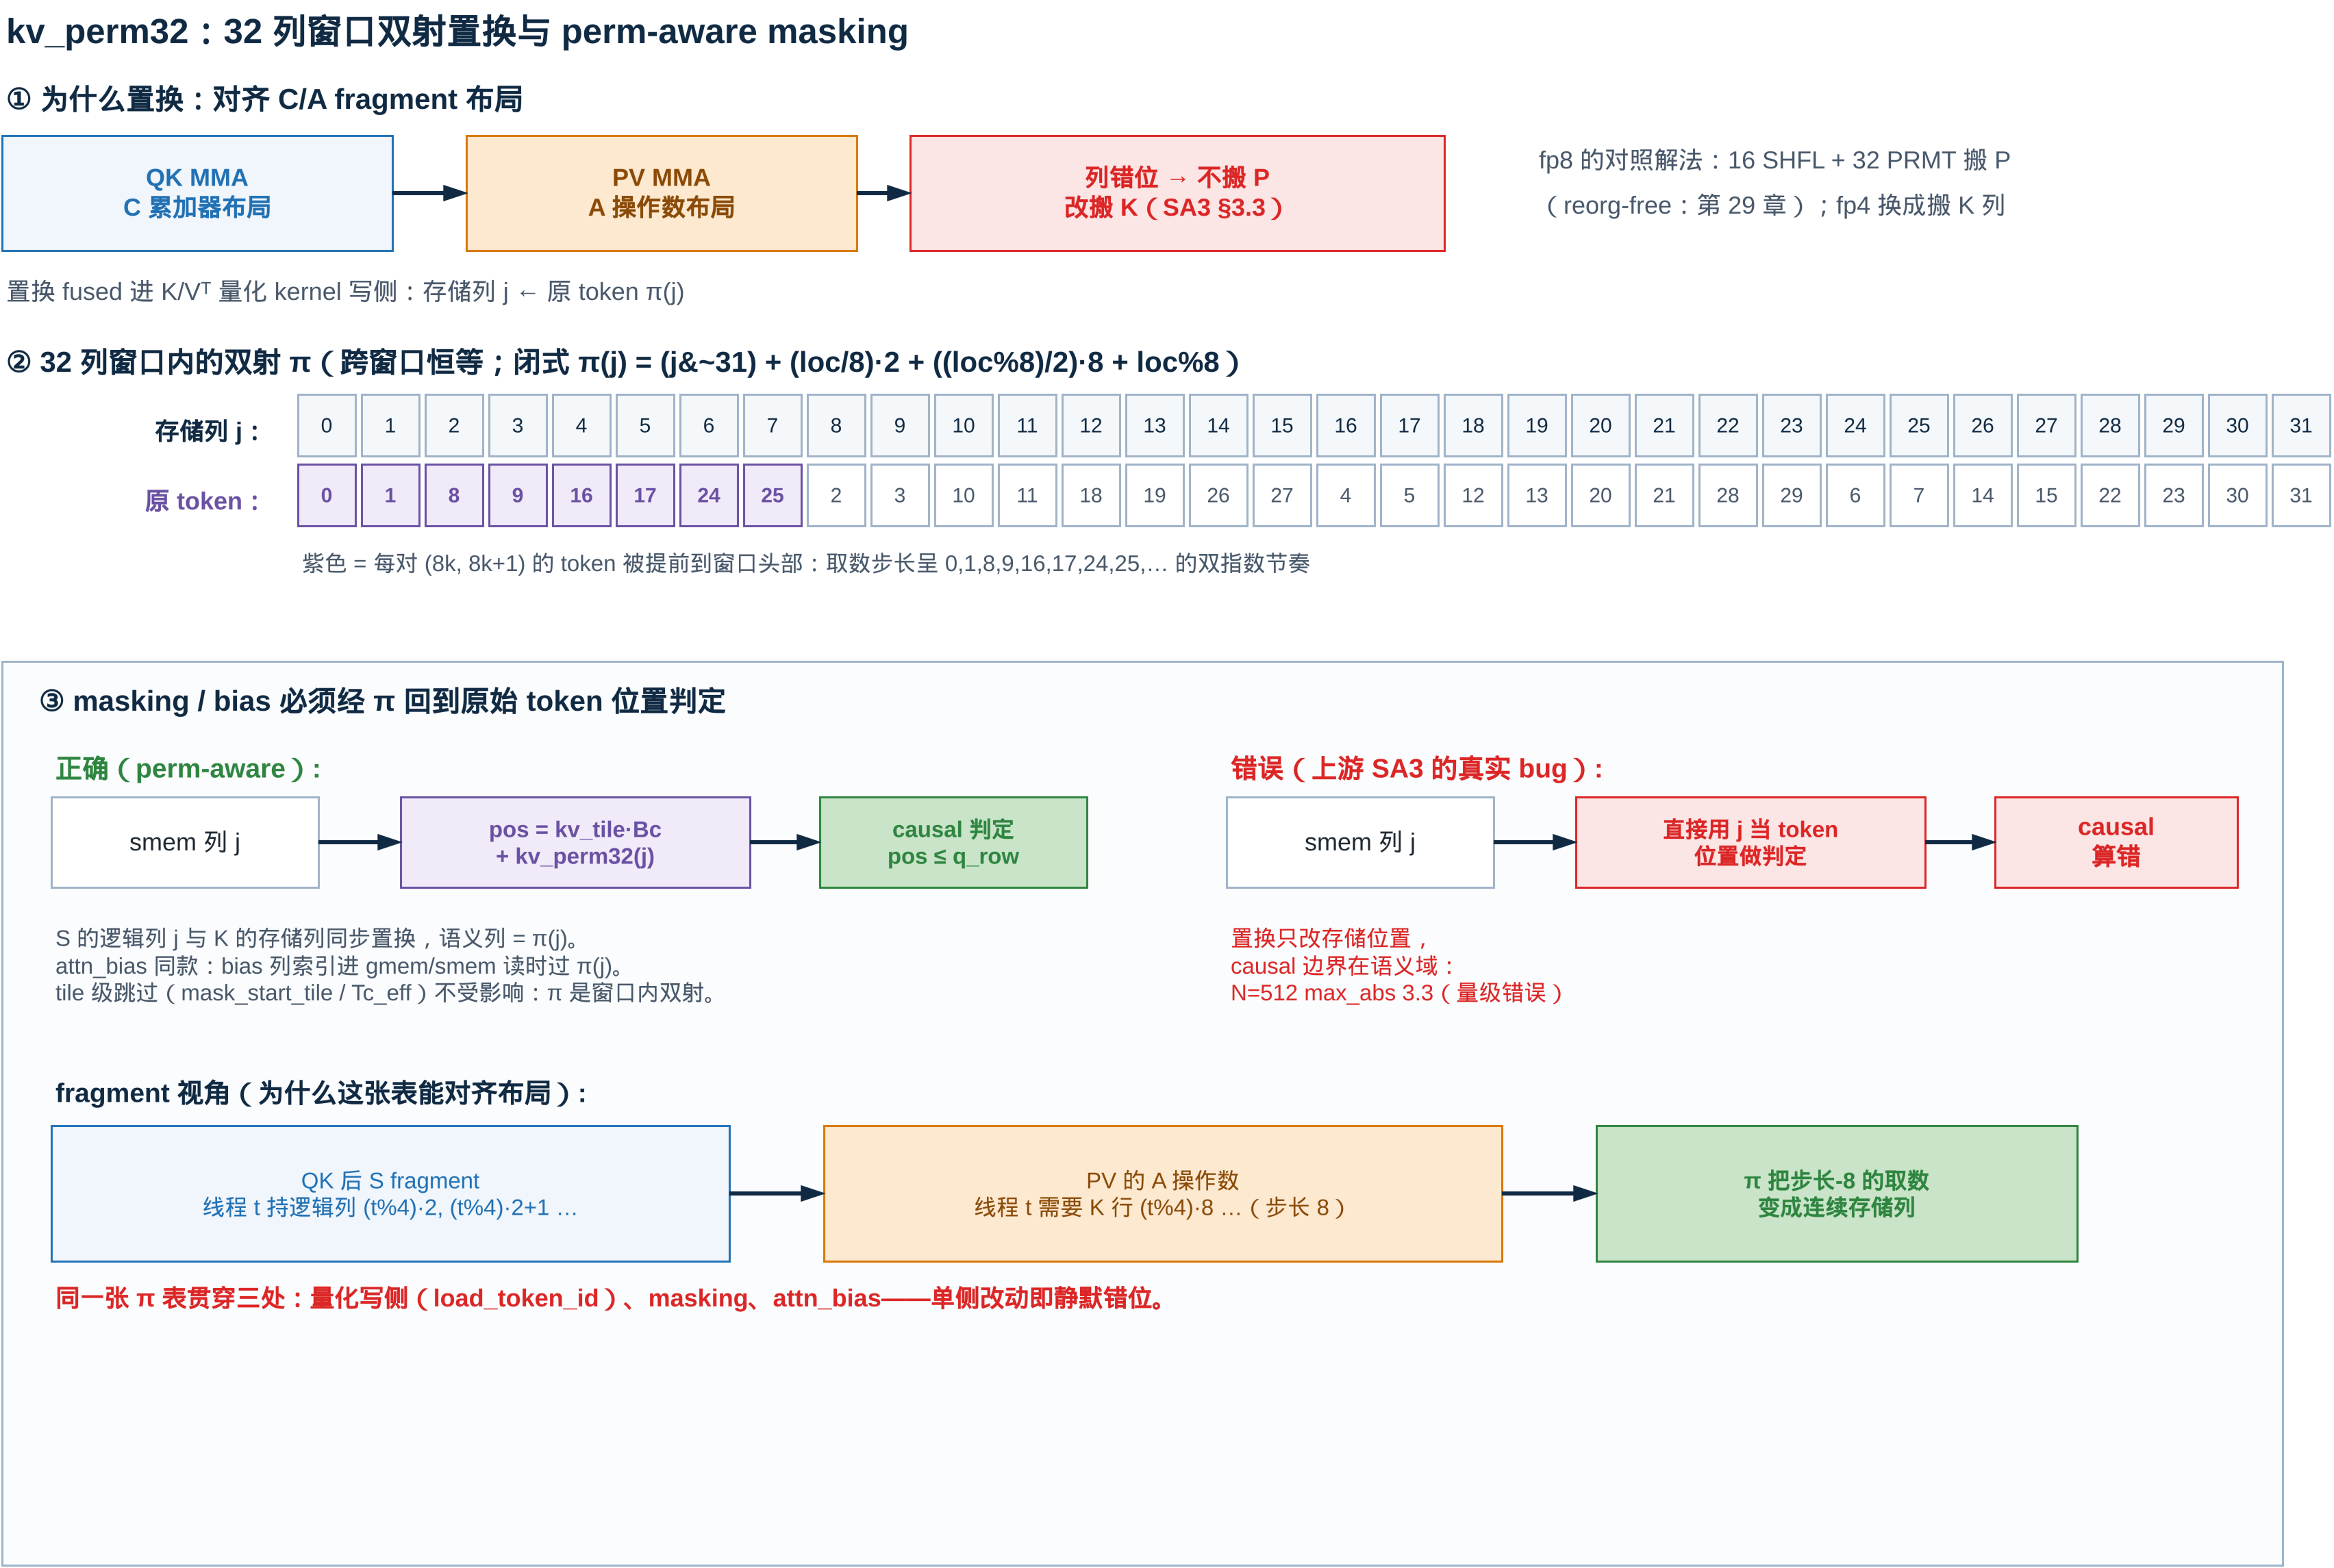
\includegraphics[width=0.98\textwidth]{figures/drawio/fig-31-3-kv-perm32/fig-31-3-kv-perm32.png}
  \begin{tikzpicture}
    \node[anchor=west, inner sep=0pt, align=left, font={\fontsize{7.4}{9.3}\selectfont \bfseries }] at (0.37,-0.354) {kv\_perm32：32 列窗口双射置换与 perm-aware masking};% w=17.094
    \node[anchor=west, inner sep=0pt, align=left, font={\fontsize{6.1}{7.7}\selectfont \bfseries }] at (0.37,-0.862) {(1) 为什么置换：对齐 C/A fragment 布局};% w=10.780
    \node[draw=tkBlue, fill=tkFillBlue, line width=0.5pt, minimum width=2.93cm, minimum height=0.86cm, inner sep=1pt, align=center, text width=2.86cm, font={\fontsize{5.2}{6.6}\selectfont \bfseries \color{tkBlue} }] at (1.833,-1.571) {QK MMA\\C 累加器布局};
    \node[draw=tkOrange, fill=tkFillOrange, line width=0.5pt, minimum width=2.93cm, minimum height=0.86cm, inner sep=1pt, align=center, text width=2.86cm, font={\fontsize{5.2}{6.6}\selectfont \bfseries \color{tkOrange!75!black} }] at (5.313,-1.571) {PV MMA\\A 操作数布局};
    \node[draw=tkRed, fill=tkFillRed, line width=0.5pt, minimum width=4.00cm, minimum height=0.86cm, inner sep=1pt, align=center, text width=3.94cm, font={\fontsize{5.2}{6.6}\selectfont \bfseries \color{tkRed} }] at (9.178,-1.571) {列错位 $\to$ 不搬 P\\改搬 K（SA3 \S{}3.3）};
    \node[anchor=west, inner sep=0pt, align=left, font={\fontsize{5.2}{6.6}\selectfont \color{black!65} }] at (11.858,-1.324) {fp8 的对照解法：16 SHFL + 32 PRMT 搬 P};% w=5.544
    \node[anchor=west, inner sep=0pt, align=left, font={\fontsize{5.2}{6.6}\selectfont \color{black!65} }] at (11.858,-1.663) {（reorg-free：第 29 章）；fp4 换成搬 K 列};% w=5.544
    \node[anchor=west, inner sep=0pt, align=left, font={\fontsize{5.2}{6.6}\selectfont \color{black!65} }] at (0.37,-2.31) {置换 fused 进 K/V$^{\top}$ 量化 kernel 写侧：存储列 j $\leftarrow$ 原 token $\pi$(j)};% w=10.780
    \node[anchor=west, inner sep=0pt, align=left, font={\fontsize{6.1}{7.7}\selectfont \bfseries }] at (0.37,-2.834) {(2) 32 列窗口内的双射 $\pi$（跨窗口恒等；闭式 $\pi$(j) = (j\&\textasciitilde{}31) + (loc/8)$\cdot$2 + ((loc\%8)/2)$\cdot$8 + loc\%8）};% w=17.094
    \node[anchor=east, inner sep=0pt, align=right, font={\fontsize{5.2}{6.6}\selectfont \bfseries }] at (2.372,-3.357) {存储列 j：};% w=2.002
    \node[anchor=east, inner sep=0pt, align=right, font={\fontsize{5.2}{6.6}\selectfont \bfseries \color{tkPurple} }] at (2.372,-3.881) {原 token：};% w=2.002
    \node[draw=gray!55, fill=black!4, line width=0.5pt, minimum width=0.43cm, minimum height=0.46cm, inner sep=1pt, align=center, text width=0.37cm, font={\fontsize{4.4}{5.5}\selectfont }] at (2.803,-3.311) {0};
    \node[draw=tkPurple, fill=tkFillPurple, line width=0.5pt, minimum width=0.43cm, minimum height=0.46cm, inner sep=1pt, align=center, text width=0.37cm, font={\fontsize{4.4}{5.5}\selectfont \bfseries \color{tkPurple} }] at (2.803,-3.835) {0};
    \node[draw=gray!55, fill=black!4, line width=0.5pt, minimum width=0.43cm, minimum height=0.46cm, inner sep=1pt, align=center, text width=0.37cm, font={\fontsize{4.4}{5.5}\selectfont }] at (3.28,-3.311) {1};
    \node[draw=tkPurple, fill=tkFillPurple, line width=0.5pt, minimum width=0.43cm, minimum height=0.46cm, inner sep=1pt, align=center, text width=0.37cm, font={\fontsize{4.4}{5.5}\selectfont \bfseries \color{tkPurple} }] at (3.28,-3.835) {1};
    \node[draw=gray!55, fill=black!4, line width=0.5pt, minimum width=0.43cm, minimum height=0.46cm, inner sep=1pt, align=center, text width=0.37cm, font={\fontsize{4.4}{5.5}\selectfont }] at (3.758,-3.311) {2};
    \node[draw=tkPurple, fill=tkFillPurple, line width=0.5pt, minimum width=0.43cm, minimum height=0.46cm, inner sep=1pt, align=center, text width=0.37cm, font={\fontsize{4.4}{5.5}\selectfont \bfseries \color{tkPurple} }] at (3.758,-3.835) {8};
    \node[draw=gray!55, fill=black!4, line width=0.5pt, minimum width=0.43cm, minimum height=0.46cm, inner sep=1pt, align=center, text width=0.37cm, font={\fontsize{4.4}{5.5}\selectfont }] at (4.235,-3.311) {3};
    \node[draw=tkPurple, fill=tkFillPurple, line width=0.5pt, minimum width=0.43cm, minimum height=0.46cm, inner sep=1pt, align=center, text width=0.37cm, font={\fontsize{4.4}{5.5}\selectfont \bfseries \color{tkPurple} }] at (4.235,-3.835) {9};
    \node[draw=gray!55, fill=black!4, line width=0.5pt, minimum width=0.43cm, minimum height=0.46cm, inner sep=1pt, align=center, text width=0.37cm, font={\fontsize{4.4}{5.5}\selectfont }] at (4.712,-3.311) {4};
    \node[draw=tkPurple, fill=tkFillPurple, line width=0.5pt, minimum width=0.43cm, minimum height=0.46cm, inner sep=1pt, align=center, text width=0.37cm, font={\fontsize{4.4}{5.5}\selectfont \bfseries \color{tkPurple} }] at (4.712,-3.835) {16};
    \node[draw=gray!55, fill=black!4, line width=0.5pt, minimum width=0.43cm, minimum height=0.46cm, inner sep=1pt, align=center, text width=0.37cm, font={\fontsize{4.4}{5.5}\selectfont }] at (5.19,-3.311) {5};
    \node[draw=tkPurple, fill=tkFillPurple, line width=0.5pt, minimum width=0.43cm, minimum height=0.46cm, inner sep=1pt, align=center, text width=0.37cm, font={\fontsize{4.4}{5.5}\selectfont \bfseries \color{tkPurple} }] at (5.19,-3.835) {17};
    \node[draw=gray!55, fill=black!4, line width=0.5pt, minimum width=0.43cm, minimum height=0.46cm, inner sep=1pt, align=center, text width=0.37cm, font={\fontsize{4.4}{5.5}\selectfont }] at (5.667,-3.311) {6};
    \node[draw=tkPurple, fill=tkFillPurple, line width=0.5pt, minimum width=0.43cm, minimum height=0.46cm, inner sep=1pt, align=center, text width=0.37cm, font={\fontsize{4.4}{5.5}\selectfont \bfseries \color{tkPurple} }] at (5.667,-3.835) {24};
    \node[draw=gray!55, fill=black!4, line width=0.5pt, minimum width=0.43cm, minimum height=0.46cm, inner sep=1pt, align=center, text width=0.37cm, font={\fontsize{4.4}{5.5}\selectfont }] at (6.145,-3.311) {7};
    \node[draw=tkPurple, fill=tkFillPurple, line width=0.5pt, minimum width=0.43cm, minimum height=0.46cm, inner sep=1pt, align=center, text width=0.37cm, font={\fontsize{4.4}{5.5}\selectfont \bfseries \color{tkPurple} }] at (6.145,-3.835) {25};
    \node[draw=gray!55, fill=black!4, line width=0.5pt, minimum width=0.43cm, minimum height=0.46cm, inner sep=1pt, align=center, text width=0.37cm, font={\fontsize{4.4}{5.5}\selectfont }] at (6.622,-3.311) {8};
    \node[draw=gray!55, fill=none, line width=0.5pt, minimum width=0.43cm, minimum height=0.46cm, inner sep=1pt, align=center, text width=0.37cm, font={\fontsize{4.4}{5.5}\selectfont \color{black!65} }] at (6.622,-3.835) {2};
    \node[draw=gray!55, fill=black!4, line width=0.5pt, minimum width=0.43cm, minimum height=0.46cm, inner sep=1pt, align=center, text width=0.37cm, font={\fontsize{4.4}{5.5}\selectfont }] at (7.099,-3.311) {9};
    \node[draw=gray!55, fill=none, line width=0.5pt, minimum width=0.43cm, minimum height=0.46cm, inner sep=1pt, align=center, text width=0.37cm, font={\fontsize{4.4}{5.5}\selectfont \color{black!65} }] at (7.099,-3.835) {3};
    \node[draw=gray!55, fill=black!4, line width=0.5pt, minimum width=0.43cm, minimum height=0.46cm, inner sep=1pt, align=center, text width=0.37cm, font={\fontsize{4.4}{5.5}\selectfont }] at (7.577,-3.311) {10};
    \node[draw=gray!55, fill=none, line width=0.5pt, minimum width=0.43cm, minimum height=0.46cm, inner sep=1pt, align=center, text width=0.37cm, font={\fontsize{4.4}{5.5}\selectfont \color{black!65} }] at (7.577,-3.835) {10};
    \node[draw=gray!55, fill=black!4, line width=0.5pt, minimum width=0.43cm, minimum height=0.46cm, inner sep=1pt, align=center, text width=0.37cm, font={\fontsize{4.4}{5.5}\selectfont }] at (8.054,-3.311) {11};
    \node[draw=gray!55, fill=none, line width=0.5pt, minimum width=0.43cm, minimum height=0.46cm, inner sep=1pt, align=center, text width=0.37cm, font={\fontsize{4.4}{5.5}\selectfont \color{black!65} }] at (8.054,-3.835) {11};
    \node[draw=gray!55, fill=black!4, line width=0.5pt, minimum width=0.43cm, minimum height=0.46cm, inner sep=1pt, align=center, text width=0.37cm, font={\fontsize{4.4}{5.5}\selectfont }] at (8.532,-3.311) {12};
    \node[draw=gray!55, fill=none, line width=0.5pt, minimum width=0.43cm, minimum height=0.46cm, inner sep=1pt, align=center, text width=0.37cm, font={\fontsize{4.4}{5.5}\selectfont \color{black!65} }] at (8.532,-3.835) {18};
    \node[draw=gray!55, fill=black!4, line width=0.5pt, minimum width=0.43cm, minimum height=0.46cm, inner sep=1pt, align=center, text width=0.37cm, font={\fontsize{4.4}{5.5}\selectfont }] at (9.009,-3.311) {13};
    \node[draw=gray!55, fill=none, line width=0.5pt, minimum width=0.43cm, minimum height=0.46cm, inner sep=1pt, align=center, text width=0.37cm, font={\fontsize{4.4}{5.5}\selectfont \color{black!65} }] at (9.009,-3.835) {19};
    \node[draw=gray!55, fill=black!4, line width=0.5pt, minimum width=0.43cm, minimum height=0.46cm, inner sep=1pt, align=center, text width=0.37cm, font={\fontsize{4.4}{5.5}\selectfont }] at (9.486,-3.311) {14};
    \node[draw=gray!55, fill=none, line width=0.5pt, minimum width=0.43cm, minimum height=0.46cm, inner sep=1pt, align=center, text width=0.37cm, font={\fontsize{4.4}{5.5}\selectfont \color{black!65} }] at (9.486,-3.835) {26};
    \node[draw=gray!55, fill=black!4, line width=0.5pt, minimum width=0.43cm, minimum height=0.46cm, inner sep=1pt, align=center, text width=0.37cm, font={\fontsize{4.4}{5.5}\selectfont }] at (9.964,-3.311) {15};
    \node[draw=gray!55, fill=none, line width=0.5pt, minimum width=0.43cm, minimum height=0.46cm, inner sep=1pt, align=center, text width=0.37cm, font={\fontsize{4.4}{5.5}\selectfont \color{black!65} }] at (9.964,-3.835) {27};
    \node[draw=gray!55, fill=black!4, line width=0.5pt, minimum width=0.43cm, minimum height=0.46cm, inner sep=1pt, align=center, text width=0.37cm, font={\fontsize{4.4}{5.5}\selectfont }] at (10.441,-3.311) {16};
    \node[draw=gray!55, fill=none, line width=0.5pt, minimum width=0.43cm, minimum height=0.46cm, inner sep=1pt, align=center, text width=0.37cm, font={\fontsize{4.4}{5.5}\selectfont \color{black!65} }] at (10.441,-3.835) {4};
    \node[draw=gray!55, fill=black!4, line width=0.5pt, minimum width=0.43cm, minimum height=0.46cm, inner sep=1pt, align=center, text width=0.37cm, font={\fontsize{4.4}{5.5}\selectfont }] at (10.919,-3.311) {17};
    \node[draw=gray!55, fill=none, line width=0.5pt, minimum width=0.43cm, minimum height=0.46cm, inner sep=1pt, align=center, text width=0.37cm, font={\fontsize{4.4}{5.5}\selectfont \color{black!65} }] at (10.919,-3.835) {5};
    \node[draw=gray!55, fill=black!4, line width=0.5pt, minimum width=0.43cm, minimum height=0.46cm, inner sep=1pt, align=center, text width=0.37cm, font={\fontsize{4.4}{5.5}\selectfont }] at (11.396,-3.311) {18};
    \node[draw=gray!55, fill=none, line width=0.5pt, minimum width=0.43cm, minimum height=0.46cm, inner sep=1pt, align=center, text width=0.37cm, font={\fontsize{4.4}{5.5}\selectfont \color{black!65} }] at (11.396,-3.835) {12};
    \node[draw=gray!55, fill=black!4, line width=0.5pt, minimum width=0.43cm, minimum height=0.46cm, inner sep=1pt, align=center, text width=0.37cm, font={\fontsize{4.4}{5.5}\selectfont }] at (11.873,-3.311) {19};
    \node[draw=gray!55, fill=none, line width=0.5pt, minimum width=0.43cm, minimum height=0.46cm, inner sep=1pt, align=center, text width=0.37cm, font={\fontsize{4.4}{5.5}\selectfont \color{black!65} }] at (11.873,-3.835) {13};
    \node[draw=gray!55, fill=black!4, line width=0.5pt, minimum width=0.43cm, minimum height=0.46cm, inner sep=1pt, align=center, text width=0.37cm, font={\fontsize{4.4}{5.5}\selectfont }] at (12.351,-3.311) {20};
    \node[draw=gray!55, fill=none, line width=0.5pt, minimum width=0.43cm, minimum height=0.46cm, inner sep=1pt, align=center, text width=0.37cm, font={\fontsize{4.4}{5.5}\selectfont \color{black!65} }] at (12.351,-3.835) {20};
    \node[draw=gray!55, fill=black!4, line width=0.5pt, minimum width=0.43cm, minimum height=0.46cm, inner sep=1pt, align=center, text width=0.37cm, font={\fontsize{4.4}{5.5}\selectfont }] at (12.828,-3.311) {21};
    \node[draw=gray!55, fill=none, line width=0.5pt, minimum width=0.43cm, minimum height=0.46cm, inner sep=1pt, align=center, text width=0.37cm, font={\fontsize{4.4}{5.5}\selectfont \color{black!65} }] at (12.828,-3.835) {21};
    \node[draw=gray!55, fill=black!4, line width=0.5pt, minimum width=0.43cm, minimum height=0.46cm, inner sep=1pt, align=center, text width=0.37cm, font={\fontsize{4.4}{5.5}\selectfont }] at (13.306,-3.311) {22};
    \node[draw=gray!55, fill=none, line width=0.5pt, minimum width=0.43cm, minimum height=0.46cm, inner sep=1pt, align=center, text width=0.37cm, font={\fontsize{4.4}{5.5}\selectfont \color{black!65} }] at (13.306,-3.835) {28};
    \node[draw=gray!55, fill=black!4, line width=0.5pt, minimum width=0.43cm, minimum height=0.46cm, inner sep=1pt, align=center, text width=0.37cm, font={\fontsize{4.4}{5.5}\selectfont }] at (13.783,-3.311) {23};
    \node[draw=gray!55, fill=none, line width=0.5pt, minimum width=0.43cm, minimum height=0.46cm, inner sep=1pt, align=center, text width=0.37cm, font={\fontsize{4.4}{5.5}\selectfont \color{black!65} }] at (13.783,-3.835) {29};
    \node[draw=gray!55, fill=black!4, line width=0.5pt, minimum width=0.43cm, minimum height=0.46cm, inner sep=1pt, align=center, text width=0.37cm, font={\fontsize{4.4}{5.5}\selectfont }] at (14.26,-3.311) {24};
    \node[draw=gray!55, fill=none, line width=0.5pt, minimum width=0.43cm, minimum height=0.46cm, inner sep=1pt, align=center, text width=0.37cm, font={\fontsize{4.4}{5.5}\selectfont \color{black!65} }] at (14.26,-3.835) {6};
    \node[draw=gray!55, fill=black!4, line width=0.5pt, minimum width=0.43cm, minimum height=0.46cm, inner sep=1pt, align=center, text width=0.37cm, font={\fontsize{4.4}{5.5}\selectfont }] at (14.738,-3.311) {25};
    \node[draw=gray!55, fill=none, line width=0.5pt, minimum width=0.43cm, minimum height=0.46cm, inner sep=1pt, align=center, text width=0.37cm, font={\fontsize{4.4}{5.5}\selectfont \color{black!65} }] at (14.738,-3.835) {7};
    \node[draw=gray!55, fill=black!4, line width=0.5pt, minimum width=0.43cm, minimum height=0.46cm, inner sep=1pt, align=center, text width=0.37cm, font={\fontsize{4.4}{5.5}\selectfont }] at (15.215,-3.311) {26};
    \node[draw=gray!55, fill=none, line width=0.5pt, minimum width=0.43cm, minimum height=0.46cm, inner sep=1pt, align=center, text width=0.37cm, font={\fontsize{4.4}{5.5}\selectfont \color{black!65} }] at (15.215,-3.835) {14};
    \node[draw=gray!55, fill=black!4, line width=0.5pt, minimum width=0.43cm, minimum height=0.46cm, inner sep=1pt, align=center, text width=0.37cm, font={\fontsize{4.4}{5.5}\selectfont }] at (15.693,-3.311) {27};
    \node[draw=gray!55, fill=none, line width=0.5pt, minimum width=0.43cm, minimum height=0.46cm, inner sep=1pt, align=center, text width=0.37cm, font={\fontsize{4.4}{5.5}\selectfont \color{black!65} }] at (15.693,-3.835) {15};
    \node[draw=gray!55, fill=black!4, line width=0.5pt, minimum width=0.43cm, minimum height=0.46cm, inner sep=1pt, align=center, text width=0.37cm, font={\fontsize{4.4}{5.5}\selectfont }] at (16.17,-3.311) {28};
    \node[draw=gray!55, fill=none, line width=0.5pt, minimum width=0.43cm, minimum height=0.46cm, inner sep=1pt, align=center, text width=0.37cm, font={\fontsize{4.4}{5.5}\selectfont \color{black!65} }] at (16.17,-3.835) {22};
    \node[draw=gray!55, fill=black!4, line width=0.5pt, minimum width=0.43cm, minimum height=0.46cm, inner sep=1pt, align=center, text width=0.37cm, font={\fontsize{4.4}{5.5}\selectfont }] at (16.647,-3.311) {29};
    \node[draw=gray!55, fill=none, line width=0.5pt, minimum width=0.43cm, minimum height=0.46cm, inner sep=1pt, align=center, text width=0.37cm, font={\fontsize{4.4}{5.5}\selectfont \color{black!65} }] at (16.647,-3.835) {23};
    \node[draw=gray!55, fill=black!4, line width=0.5pt, minimum width=0.43cm, minimum height=0.46cm, inner sep=1pt, align=center, text width=0.37cm, font={\fontsize{4.4}{5.5}\selectfont }] at (17.125,-3.311) {30};
    \node[draw=gray!55, fill=none, line width=0.5pt, minimum width=0.43cm, minimum height=0.46cm, inner sep=1pt, align=center, text width=0.37cm, font={\fontsize{4.4}{5.5}\selectfont \color{black!65} }] at (17.125,-3.835) {30};
    \node[draw=gray!55, fill=black!4, line width=0.5pt, minimum width=0.43cm, minimum height=0.46cm, inner sep=1pt, align=center, text width=0.37cm, font={\fontsize{4.4}{5.5}\selectfont }] at (17.602,-3.311) {31};
    \node[draw=gray!55, fill=none, line width=0.5pt, minimum width=0.43cm, minimum height=0.46cm, inner sep=1pt, align=center, text width=0.37cm, font={\fontsize{4.4}{5.5}\selectfont \color{black!65} }] at (17.602,-3.835) {31};
    \node[anchor=west, inner sep=0pt, align=left, font={\fontsize{4.8}{6.0}\selectfont \color{black!65} }] at (2.587,-4.343) {紫色 = 每对 (8k, 8k+1) 的 token 被提前到窗口头部：取数步长呈 0,1,8,9,16,17,24,25,\ldots{} 的双指数节奏};% w=15.246
    \node[draw=gray!55, fill=black!2, line width=0.5pt, minimum width=17.09cm, minimum height=6.78cm, inner sep=1pt, align=center, text width=17.03cm, font={\fontsize{5.7}{7.1}\selectfont }] at (8.917,-8.47) {};
    \node[anchor=west, inner sep=0pt, align=left, font={\fontsize{6.1}{7.7}\selectfont \bfseries }] at (0.616,-5.375) {(3) masking / bias 必须经 $\pi$ 回到原始 token 位置判定};% w=16.478
    \node[anchor=west, inner sep=0pt, align=left, font={\fontsize{5.7}{7.1}\selectfont \bfseries \color{tkGreen!70!black} }] at (0.739,-5.883) {正确（perm-aware）:};% w=7.700
    \node[draw=gray!55, fill=none, line width=0.5pt, minimum width=2.00cm, minimum height=0.68cm, inner sep=1pt, align=center, text width=1.94cm, font={\fontsize{5.2}{6.6}\selectfont }] at (1.74,-6.437) {smem 列 j};
    \node[draw=tkPurple, fill=tkFillPurple, line width=0.5pt, minimum width=2.62cm, minimum height=0.68cm, inner sep=1pt, align=center, text width=2.56cm, font={\fontsize{4.8}{6.0}\selectfont \bfseries \color{tkPurple} }] at (4.666,-6.437) {pos = kv\_tile$\cdot$Bc\\+ kv\_perm32(j)};
    \node[draw=tkGreen, fill=tkFillGreen, line width=0.5pt, minimum width=2.00cm, minimum height=0.68cm, inner sep=1pt, align=center, text width=1.94cm, font={\fontsize{4.8}{6.0}\selectfont \bfseries \color{tkGreen!70!black} }] at (7.5,-6.437) {causal 判定\\pos $\leq$ q\_row};
    \node[anchor=west, inner sep=0pt, align=left, font={\fontsize{4.8}{6.0}\selectfont \color{black!65} }] at (0.739,-7.361) {S 的逻辑列 j 与 K 的存储列同步置换，语义列 = $\pi$(j)。\\attn\_bias 同款：bias 列索引进 gmem/smem 读时过 $\pi$(j)。\\tile 级跳过（mask\_start\_tile / Tc\_eff）不受影响：$\pi$ 是窗口内双射。};% w=8.008
    \node[anchor=west, inner sep=0pt, align=left, font={\fontsize{5.7}{7.1}\selectfont \bfseries \color{tkRed} }] at (9.548,-5.883) {错误（上游 SA3 的真实 bug）:};% w=7.700
    \node[draw=gray!55, fill=none, line width=0.5pt, minimum width=2.00cm, minimum height=0.68cm, inner sep=1pt, align=center, text width=1.94cm, font={\fontsize{5.2}{6.6}\selectfont }] at (10.549,-6.437) {smem 列 j};
    \node[draw=tkRed, fill=tkFillRed, line width=0.5pt, minimum width=2.62cm, minimum height=0.68cm, inner sep=1pt, align=center, text width=2.56cm, font={\fontsize{4.8}{6.0}\selectfont \bfseries \color{tkRed} }] at (13.475,-6.437) {直接用 j 当 token\\位置做判定};
    \node[draw=tkRed, fill=tkFillRed, line width=0.5pt, minimum width=1.82cm, minimum height=0.68cm, inner sep=1pt, align=center, text width=1.76cm, font={\fontsize{5.2}{6.6}\selectfont \bfseries \color{tkRed} }] at (16.216,-6.437) {causal\\算错};
    \node[anchor=west, inner sep=0pt, align=left, font={\fontsize{4.8}{6.0}\selectfont \color{tkRed} }] at (9.548,-7.361) {置换只改存储位置，\\causal 边界在语义域：\\N=512 max\_abs 3.3（量级错误）};% w=7.700
    \node[anchor=west, inner sep=0pt, align=left, font={\fontsize{5.7}{7.1}\selectfont \bfseries }] at (0.739,-8.316) {fragment 视角（为什么这张表能对齐布局）:};% w=16.478
    \node[draw=tkBlue, fill=tkFillBlue, line width=0.5pt, minimum width=5.08cm, minimum height=1.02cm, inner sep=1pt, align=center, text width=5.02cm, font={\fontsize{4.8}{6.0}\selectfont \color{tkBlue} }] at (3.28,-9.071) {QK 后 S fragment\\线程 t 持逻辑列 (t\%4)$\cdot$2, (t\%4)$\cdot$2+1 \ldots{}};
    \node[draw=tkOrange, fill=tkFillOrange, line width=0.5pt, minimum width=5.08cm, minimum height=1.02cm, inner sep=1pt, align=center, text width=5.02cm, font={\fontsize{4.8}{6.0}\selectfont \color{tkOrange!75!black} }] at (9.071,-9.071) {PV 的 A 操作数\\线程 t 需要 K 行 (t\%4)$\cdot$8 \ldots{}（步长 8）};
    \node[draw=tkGreen, fill=tkFillGreen, line width=0.5pt, minimum width=3.60cm, minimum height=1.02cm, inner sep=1pt, align=center, text width=3.54cm, font={\fontsize{4.8}{6.0}\selectfont \bfseries \color{tkGreen!70!black} }] at (14.122,-9.071) {$\pi$ 把步长-8 的取数\\变成连续存储列};
    \node[anchor=west, inner sep=0pt, align=left, font={\fontsize{5.2}{6.6}\selectfont \bfseries \color{tkRed} }] at (0.739,-9.856) {同一张 $\pi$ 表贯穿三处：量化写侧（load\_token\_id）、masking、attn\_bias------单侧改动即静默错位。};% w=16.478
    \draw[black!75, line width=0.8pt, -{Stealth[length=2.2pt,width=1.8pt]}] (3.296,-1.571) -- (3.85,-1.571);
    \draw[black!75, line width=0.8pt, -{Stealth[length=2.2pt,width=1.8pt]}] (6.776,-1.571) -- (7.176,-1.571);
    \draw[black!75, line width=0.8pt, -{Stealth[length=2.2pt,width=1.8pt]}] (2.741,-6.437) -- (3.357,-6.437);
    \draw[black!75, line width=0.8pt, -{Stealth[length=2.2pt,width=1.8pt]}] (5.975,-6.437) -- (6.499,-6.437);
    \draw[black!75, line width=0.8pt, -{Stealth[length=2.2pt,width=1.8pt]}] (11.55,-6.437) -- (12.166,-6.437);
    \draw[black!75, line width=0.8pt, -{Stealth[length=2.2pt,width=1.8pt]}] (14.784,-6.437) -- (15.308,-6.437);
    \draw[black!75, line width=0.8pt, -{Stealth[length=2.2pt,width=1.8pt]}] (5.821,-9.071) -- (6.53,-9.071);
    \draw[black!75, line width=0.8pt, -{Stealth[length=2.2pt,width=1.8pt]}] (11.612,-9.071) -- (12.32,-9.071);
  \end{tikzpicture}
  \caption{kv\_perm32 的 32 列窗口双射与 perm-aware masking。置换让
  QK 的 C fragment 列直接匹配 PV 的 A 操作数布局；mask/bias 必须经
  \label{fig:31-3}
  $\pi^{-1}$ 回到原始 token 位置判定。}
\end{figure}

\FloatBarrier

\section{性能分析}

\subsection{量化链本身的收益}

$\Delta S$ 的 wmma kernel 替换 torch 链（bmm + transpose copy +
epilogue cast）是大头：$N{=}16384$ 级别从 $\sim$1.4ms 降到
$\sim$0.3ms（\texttt{.tmp/book-bench/} 历史记录；头注释 L6--8 只记
旧链 $\sim$1ms 量级）。
fused WHT 是「零成本旋钮」的典范：D=128 实测
\texttt{--fp4-hadamard} 与基线 2.52/1.67ms 完全一致（表~\ref{tab:31-knobs}）——旋转折进 load 路径后，
quantize kernel 的瓶颈（gmem 带宽）没有变。

\begin{table}[H]
  \centering
  \caption{fp4 量化链 knob A/B（PRO 5000，$B{=}1,H{=}32,N{=}8192,D{=}128$，
  self/causal，fp16 口径；数据落盘 \texttt{.tmp/book-bench/ch31/}）}
  \label{tab:31-knobs}
  \begin{tabular}{@{}lllll@{}}
    \toprule
    配置 & self (ms) & causal (ms) & self vs 基线 & allclose \\
    \midrule
    基线（强制 smooth-Q/K） & 2.52 & 1.67 & --- & 全 $\checkmark$ \\
    \texttt{--fp4-hadamard} & 2.52 & 1.67 & $\pm$0\% & 全 $\checkmark$ \\
    \texttt{--fp4-smooth-v} 组合 & 2.59 & 1.75 & $+2.8\%$ & 全 $\checkmark$ \\
    \texttt{--fp4-pv-mm-type fp8} & 3.47 & 2.17 & $+37.7\%$ & 全 $\checkmark$ \\
    \bottomrule
  \end{tabular}
\end{table}

MXFP8 PV 变体（$V^\top$ 走 e4m3 + ue8m0/32，精度更高）付出 37.7\%
的 self 时间代价：V 侧数据带宽翻倍（8 bit vs 4 bit）、MMA atom 从
\texttt{m16n32k64} 换 \texttt{m16n8k128}，两者吞吐相近但带宽劣势直
接体现在 e2e。它存在的意义是精度保险丝（$D\le192$ 才有 smem 预算，
\texttt{attn\_traits.cuh} L58--63），不是性能选项。

\subsection{e2e：fp4 persist-D 的 D 扫描}

\begin{table}[H]
  \centering
  \caption{fp4 persist-D e2e bench（PRO 5000，$B{=}1,H{=}32,N{=}8192$；
  tol：dense 0.15 / causal 0.70，16 格全绿）}
  \label{tab:31-bench}
  \begin{tabular}{@{}rlllll@{}}
    \toprule
    $D$ & self FFPA/SDPA (ms) & 吞吐 & causal FFPA/SDPA (ms) & 吞吐 & 加速比区间 \\
    \midrule
    64  & 1.61 / 2.40 & 341T & 1.08 / 1.35 & 255T & 1.23--1.49x \\
    128 & 2.52 / 5.11 & 437T & 1.67 / 2.68 & 330T & 1.61--2.03x \\
    192 & 3.48 / 7.14 & 474T & 2.40 / 3.81 & 344T & 1.59--2.05x \\
    256 & 4.97 / 10.46 & 443T & 3.54 / 5.27 & 311T & 1.49--2.11x \\
    \bottomrule
  \end{tabular}
\end{table}

三个观察：(1) fp4 的 e2e 加速比区间（1.2--2.1x）整体高于同机 fp8
persist-D（第~\ref{ch:29}~章表 29.2 的 1.26--1.70x），来源不是 MMA
吞吐——blockscale mxf4nvf4 的吞吐只与 fp8 dense 相当——而是
\textbf{带宽}：K/V/SF 的字节数减半以上，memory-bound 的 attention
直接受益（skill §6.6：attn kernel 本身快 $\sim$23\%）。(2) D=192 的
474T 是全家族峰值，D=256 回落（kStages 从 3 降 2，L51--56）。(3)
$\sim$1ms 量级的前处理链意味着\textbf{小 $N_q$（cross/decode）结构
性不划算}——以 $D{=}192$（e2e 3.48ms）计占比约 30\%；$N_q$ 缩小
时主 kernel 按 $N_q\cdot N_{kv}$ 缩、前处理几乎不缩，占比急速恶
化。

\section{实践经验}

\textbf{移植策略：fragment adapter 逐字拷贝}。kv\_perm32 体系、SF
atom 布局、C/A fragment 映射这些内容是 SA3 在真实 hardware 上调试出
来的位级布局知识，重写极易引入静默错位。ffpa 的选择是逐字拷贝
adapter 层、自研外闱（骨架/pipeline/dispatch），只修正确性 bug
（perm-aware masking）。这与第~\ref{ch:28}--\ref{ch:29}~章自研 fp8
链的策略不同——fp8 没有 SA3 级别的现成参照。

\textbf{评估口径}。fp4 的 max\_abs 在 causal 尖峰行天然 0.5--0.75
（e2m1 的 25\% 步长 × 尖峰行 P 近 one-hot 的误差结构，probe sim 与
kernel 同级证明是格式固有），SA3 论文自身用 cosine 评估。工程验收
应该看 mean\_abs（0.014--0.03 是质量指标）与 allclose 容差
（dense 0.15 / causal 0.70），不要用 fp8 的 0.05 级容差去卡 fp4。

\textbf{固定链的适用边界}。本节 bench 都是 $N_q{=}8192$；把 fp4 路径
用在 decode/短序列上，前处理链的固定成本会吞掉全部收益。规划上应把
fp4 前处理与 prefill 阶段绑定，decode 回 fp8/fp16 路径。

\section{常见坑}

\begin{enumerate}[itemsep=2pt,topsep=2pt]
  \item \textbf{subbyte 指针}：\texttt{reinterpret\_cast<Element*>} 对
        4 bit 类型按 1B 缩放偏移，地址差 2 倍，TMA IMA 在
        stage$\ge$1 才爆——必须 \texttt{make\_smem\_ptr}（31.4.6 节）。
  \item \textbf{0/0 NaN}：全零块 $s=0$，除法前必须特判倒数取 0
        （L293/L460）；全 masked 组、pad 列都会触发。
  \item \textbf{masking 不 perm-aware}：置换存储后 causal 谓词忘了过
        $\pi^{-1}$，max\_abs 直接 3.3 级别（上游 SA3 的真实 bug）。
  \item \textbf{SF 写序不 match atom}：SF offset 公式与
        \texttt{BlockScaledConfig} 不一致时数据看起来「差不多对」但
        精度崩——SF 错位是尺度级错误，不是噪声级。
  \item \textbf{e2m1 的饱和语义}：\texttt{cvt.rn.satfinite.e2m1x2.f32}
        的 \texttt{.satfinite} 是 PTX 对 4 bit 目的端的强制修饰符（不
        存在非 satfinite 的裸变体），越界值饱和到 $\pm$6、NaN 转 $+6$，
        均不产 NaN；真正的风险在绕开 \texttt{cvt} 的手搓编码（无饱和
        语义）与上游 0/0（见坑 2），不在 \texttt{cvt} 本身（L41/L64）。
  \item \textbf{mxfp8 的 stage 数学史}：早期 build 因一次 3-stage
        D=128 NaN 把全部 D 钉在 2 stage；后来定位不复现（16 shape 组合
        + 5 次新数据复测全无 NaN），D=128 恢复 3 stage 拿回 1.2\% kernel
        时间（\texttt{attn\_traits.cuh} L56--62）。教训：一次异常
        触发的保守回退要有复测机制，否则永久付性能税。
\end{enumerate}

\section{面试要点速查}

\begin{enumerate}[itemsep=2pt,topsep=2pt]
  \item NVFP4 vs MXFP4：同为 e2m1 数据，SF 分别是 ue4m3/16 块与
        ue8m0/32 块；SF 尾数位决定尺度精度，MXFP4 的整数 SF 步长
        100\%。
  \item blockscale MMA 语义：data+SF 双操作数，dequant 逐块隐含在
        累加里；SF 自身的 ue4m3 舍入（6.25\%）整体作用于块。
  \item 为什么 fp4 强制 smooth：e2m1 ±6 域下均值偏移吃掉
        $\mathrm{amax}$ 预算；fp8 可以选、fp4 必须。
  \item $\Delta S$ 恒等式：$q_m(K-\bar k)^\top=q_mK^\top-q_{km}$，
        免物化 $K-\bar k$；多余行常数平移 lse 不改 $O$。
  \item smooth-V 精确性：softmax 权重和为 1 $\Rightarrow$ 减均值是恒等变换，
        只收动态范围。
  \item kv\_perm32：为对齐 C/A fragment 布局置换 K 列（32 列窗口双
        射）；mask/bias 必须 perm-aware，tile 级公式不受影响。
  \item fused WHT 的蝶形拆分：thread-local 对原地做，只剩两级
        \texttt{shfl\_xor}；均值/旋转可交换 $\Rightarrow$ $\Delta S$ 留在未旋转
        域。
\end{enumerate}

\section{最小测试与动手实验}

bench 环境沿用第~\ref{ch:28}~章约定（卡 7、\texttt{cdit} 环境，
小 D 需开环境变量），输出落盘 \texttt{.tmp/book-bench/ch31/}：

\begin{lstlisting}[style=console]
export CUDA_VISIBLE_DEVICES=7 FFPA_CUDA_ALLOW_SMALL_D=1
python -m ffpa_attn.bench --fwd-backend cuda --cuda-impl fp4 \
  --tasks self-attn causal --D 128 --no-bwd --show-allclose
# 变体：
#   --fp4-hadamard            # fused WHT（零开销验证）
#   --fp4-smooth-v            # V 均值减除
#   --fp4-pv-mm-type fp8      # MXFP8 PV（D<=192）
\end{lstlisting}

\begin{enumerate}[itemsep=2pt,topsep=2pt]
  \item \textbf{D 扫描复现}：$D\in\{64,128,192,256\}$ 复现
        表~\ref{tab:31-bench}；解释 D=256 吞吐回落（kStages 3$\to$2）。
  \item \textbf{hadamard 零开销}：A/B \texttt{--fp4-hadamard}，确认
        self/causal 时间在噪声内一致；再开非 pow2 D（如 192）观察它
        回退到独立 WHT kernel 后的额外成本。
  \item \textbf{MXFP8 PV 边界}：$D\in\{128,192,256\}$ 试
        \texttt{--fp4-pv-mm-type fp8}，验证 256 被 smem 预算拒绝。
  \item \textbf{读恒等式}：对照 \texttt{delta\_s.cuh} L3--8 与
        \texttt{quantize\_fp4.cuh} L437--455 的两段注释，手推
        式~\ref{eq:31-deltas-id} 与~\ref{eq:31-smoothv}。
\end{enumerate}

\section*{延伸阅读}
\addcontentsline{toc}{section}{延伸阅读}

\begin{itemize}[itemsep=0pt,topsep=2pt]
  \item \texttt{cute/fp4/quantize\_fp4.cuh} 头注释（L1--14）：SA3
        移植边界与 padding 契约；
  \item \texttt{cute/fp4/delta\_s.cuh} 头注释（L1--18）：rank-1 恒等式
        与 memory-bound 判断；
  \item \texttt{cute/fp4/fp4\_gemm.cuh}（L24--30）：kv\_perm32 闭式与
        perm-aware bias 注入；
  \item \texttt{cute/fp4/attn\_traits.cuh}（L51--63）：kStages 的 smem
        预算推导与 mxfp8 stage 史；
  \item SageAttention3 论文 §3.1--3.3（NVFP4 格式、两级 P 量化、K
        置换）；两级 P 量化的数学与实现见本书第~\ref{ch:32}~章。
\end{itemize}

% ch32-fp4-persist-d.tex — FP4(二)：persist-D 主 kernel 与两级 P 量化（RFC-K6）★
% 源码：ffpa-attn(861d75e) cute/fp4/sm_120/persist_d.cuh(1113L) + fp4_pscale.cuh(793L) + fp4_gemm.cuh(276L)
\chapter{FP4（二）：persist-D 主 Kernel 与两级 P 量化}\label{ch:32}

\section{本章导读}

第~\ref{ch:31}~章把 Q/K/V 送进了 e2m1 + ue4m3 的 workspace；本章讲
消费它们的\textbf{主 kernel}：
\texttt{fp4\_persist\_d\_fwd\_}\allowbreak\texttt{cute\_fp4\_sm120}
（\texttt{sm\_120/persist\_d.cuh}，1113 行），跑在 fp8 persist-D 同款
128 线程 producer + 256 线程 consumer 的 warp-specialized 骨架上
（第~\ref{ch:29}~章），数据路径移植自 SageAttention3 的 NVFP4 kernel。

本章的主角是\textbf{两级 P 量化}——SA3 对「$P$ 无法离线校准」这一挑战
的回答，也是 fp4 attention 精度成立的最后一块拼图。它不是独立的
pass，而是与 online softmax \textbf{融合}在一起的
（\texttt{fp4\_pscale.cuh} 的 \texttt{SoftmaxFused}）：softmax 吐出的
每个数直接落进第二级量化的域，$s_{P1}$ 的常数折进 \texttt{exp2} 的
shift，除法和归一化在到达寄存器之前就已经消失。

\section{问题与动机}

\textbf{P 的三重困境}。Q/K/V 的量化无论多粗，都可以离线统计
（smooth、per-block scale）压动态范围；$P$ 不行：
\begin{enumerate}[itemsep=0pt,topsep=2pt]
  \item \textbf{online}：$P$ 是 softmax 现场产物，kernel 内逐 tile 生成，
        没有第二遍数据；
  \item \textbf{值域窄}：$P\in[0,1]$，且行内分布剧变——causal 早期行
        近 one-hot（一个 1、其余 $\approx0$），dense 行近均匀且数值极小；
  \item \textbf{SF 格式自身的损耗}（SA3 的 C2 挑战）：若按块直接量化，
        $s_P=\mathrm{amax}(P_{块})/6\in[0,0.167]$，ue4m3 在这个窄域的
        有效位数被浪费——\textbf{尺度因子自己}先损失精度，再乘回 16
        个元素。
\end{enumerate}
两级量化的思路：先把整行线性拉伸到 NVFP4 的满量程（第一级，全局
常数），块内再用 e2m1 域归一（第二级，per-16 组 ue4m3）——让块的
$\mathrm{amax}$ 恰好铺满 ue4m3 的域。

\textbf{硬件侧的结构约束}。blockscale MMA
（\texttt{m16n32k64 kind::mxf4nvf4}，\texttt{attn\_traits.cuh} L77）要
求 K 维 64 对齐、SF 以 \texttt{scale\_vec::4X} 旁路喂入；P 作为 A 操作
数必须以 data+SF 的 zip 形式出现（\texttt{fp4\_pscale.cuh} L314--346 的
pack 注释）。这套约束决定了 P 量化必须发生在寄存器里、紧贴 MMA。

\section{数学原理}

\subsection{两级 P 量化：SA3 §3.2 的方案}

对 softmax 输出 $\tilde P$（已减行 max、未归一），两级量化定义为：
\begin{equation}
  s_{P1}[row]=\frac{\mathrm{rowmax}(\tilde P)}{448\times6},\qquad
  \tilde P_2=\frac{\tilde P}{s_{P1}}\in[0,\,2688],\qquad
  \hat P_2,s_{P2}=\phi(\tilde P_2)
  \label{eq:32-two-level}
\end{equation}
$2688=448\times6$：分子是 ue4m3 满量程、分母是 e2m1 满量程，第一级把
行拉伸到「SF 与数据的乘积极限域」。dequant 端
$O=\mathrm{FP4MM}(\hat P_2,s_{P2},\hat V,s_V)\times s_{P1}$，常数
$s_{P1}$ 在 $O$ 与 row\_sum 中\textbf{同现同消}——finalize 相除后精确
抵消（\texttt{fp4\_pscale.cuh} L327--330 注释）。

\subsection{online softmax 下的退化：第一级变成常数}

ffpa 实现的关键洞察（\texttt{fp4\_pscale.cuh} 头注释 L2--5）：online
softmax 对当前 tile 已经减去运行行 max，所以
$\mathrm{rowmax}(\tilde P)\equiv1$，逐行的 $s_{P1}$ \textbf{退化为全
局常数} $1/(448\times6)$，可以直接折进 \texttt{exp2} 的 shift：
\begin{equation}
  P_2=\exp_2\!\bigl(S\cdot L-m\cdot L+\log_2(448\cdot6)\bigr)
  \in[0,\,2688],\qquad
  s_{P2}=\exp_2\!\bigl(a\cdot L-m_{sc}+\log_2\tfrac{1}{6}\bigr)\in(0,\,448]
  \label{eq:32-p2-domain}
\end{equation}
其中 $L=\mathrm{scale}\cdot\log_2 e$，$a$ 是 16 元素组 absmax，$m_{sc}$
是含第一级常数的行 max（L117--119 注释与 L126--128 的三个编译期
常数：$\log_2(1/2688)=-11.3923$、$\log_2(1/6)=-2.5850$）。第一级量化
的除法、$s_{P1}$ 的存储与乘回全部消失。常数符号容易看错：
$m_{sc}=m\cdot L+\log_2\frac{1}{2688}$，减去它等效加上
$\log_2 2688$，所以 $s=m$ 时 $P_2$ 恰达 $2688$（源码注释 L118 把
shift 写作 $+\log_2(1/(448\cdot6))$，是同款符号笔误，以代码与值域为
准）。

\subsection{归一化也折进 exp2}

第二级本需要 $q=\tilde P_2/s_{P2}$（数据除以组尺度才能落 e2m1 域）。
实现把这一步同样折进指数（L182--186 注释）：
\begin{equation}
  q=\exp_2\!\bigl((s-a)\cdot L+\log_2 6\bigr)\in(0,\,6]
\end{equation}
组 absmax 归一化在 \texttt{exp2} 参数里完成，\textbf{rcp 与逐元素
FMUL 在 softmax 与 pack 之间整段消失}；row\_sum 用 FMA 吸收 $s_{P2}$
因子（\texttt{row\_sum = fmaf(q, sfp2, row\_sum)}，L195）。硬件只要
一条 MUFU.EX2——\texttt{ex2.approx.ftz.f32} 的 \texttt{.ftz} 让 ptxas
不必包 range glue（L21--22 注释，非 ftz 形式每次调用要多出 FSETP/
FSEL/FMUL 链，实测 -5.9\%）。

\textbf{同一条 shuffle 链做两个归约}：C fragment 每 lane 持 8 元素，
$\texttt{shfl\_xor}(1)$ 合成 16 元素组 absmax，$\texttt{shfl\_xor}(2)$
完成 quad 内行 max（L160--167）——组尺度和行 max 的冗余
归约减半。

\textbf{全 masked 组的退化}：$a=-\infty$ 时特判 $a\to0$（L187 的
\texttt{a\_arg} clamp），$q$ 与 row\_sum 贡献双双归 0 而不是 NaN；
\texttt{InfCheck} 模板参数处理整行有效列全部落在当前 tile 之外的
causal 左上角（L169--175、L219--221 的 \texttt{scores\_max\_cur} 守卫）。

\subsection{lazy rescale 与 lse 复合公式}

跨 tile 的行 max 更新沿用 fp8 的 lazy rescale（第~\ref{ch:29}~章）：
$O$ 不即时重缩放，记 \texttt{scores\_scale}，下一个 tile 的 PV 累加前
按行补乘（\texttt{rescale\_acc}，L299；PC-11 起为 per-row 守卫——
\texttt{scores\_scale(mi)<1.0f} 的行跳过 FMUL，dense 路径 96.5\% 命中
零开销，\texttt{persist\_d.cuh} L968--975 注释）。

lse 的复合公式（每项都有出处）：
\begin{equation}
  \mathrm{lse}=\bigl(m\cdot L+\log_2(\mathrm{row\_sum})+
  \log_2\tfrac{1}{2688}\bigr)\ln 2+\mathrm{scale}\cdot q_{km}
  \label{eq:32-lse}
\end{equation}
第一项是 log2 域行 max 与 row\_sum，第三项是两级量化的 $1/2688$ 因子
（行和处于 $P\cdot2688$ 域，要除回来），最后一项是 smooth-K 的修正
$\mathrm{dot}(q_{row},\bar k)$（第~\ref{ch:31}~章
式~31-deltas 的对应项；\texttt{lse\_qkm\_dot} 在 Q 寄存器拷贝后、kv
循环之前算好，L583--591 与 \texttt{persist\_d.cuh} L757--758——Q 的
smem 在 \texttt{kQSmemReuse} 下会被 V stage 复用，点积必须提前）。

\subsection{MXFP8 PV 变体的数值契约}

\texttt{--fp4-pv-mm-type fp8} 把 $V^\top$ 换成 e4m3 + ue8m0（32 元素
组），P 侧同样换 32 粒度两级量化：域常量从 2688 换成 $448$（e4m3 满
量程，无第二级 e2m1 因子），SF 是 2 的幂
（\texttt{pow2\_to\_ue8m0}，L417；契约注释 L390--397）。SFA 的槽位排
布按 \texttt{SM120\_16x8x128\_TN\_VS\_MXFP8} atom 的 A 布局走
（L501--535 的 probe 结论）。历史上 MXFP8 PV 的 lse 曾无条件沿用
2688 域——差 $\ln 6$ 的 latent bug，现按 \texttt{kPvMxfp8} 编译期分
流。

\section{设计与实现}

\subsection{骨架复用与 grid 调度契约}

WS 骨架与 fp8 persist-D 同构：128T producer（TMA 装载 K/V/SF/bias）+
256T consumer（8 warp MMA），4 组反向 barrier
（\texttt{k\_empty}/\texttt{v\_empty}/\texttt{q\_consumed}/
\texttt{epilogue\_done}，L200--213 注释）。fp4 特有的协议纪律：所有
mbarrier \textbf{永不 re-initialize}——per-CTA 全局 kv-tile 计数器驱动
每个 barrier 的 stage/phase 跨 work 连续翻转（对活跃 mbarrier 的
re-init 是 UB，PTX ISA 9.7.13.15.9；L113--115、L316 注释）。

grid 调度契约是「\textbf{单 kernel、单代码路径、runtime grid 定风格}」
（L92--120 注释）：kernel 体是
\texttt{for (work\_id = blockIdx.x; work\_id < total\_work; work\_id +=
gridDim.x)} 的 strided work loop。dense 用
$\min(total\_work, SMs)$（persistent，流水 fill/drain 每 CTA 摊一次，
producer 可在 consumer 跑 epilogue 时预取下一个 work 的 K/V）；causal
用 \texttt{total\_work}（经典 block-per-work，短 work 早完早释放 SM，
HW 调度器负载均衡——多数 work 的 $T_{c,eff}\ll T_c$，persistent 的
每 work 固定开销会占主导）。barrier 协议对任意 gridDim 都成立，
non-persistent 只是每 barrier 只翻第一个 phase 的退化情形。

\subsection{Q 的寄存器驻留与一个教科书级 bug}

Q/SFQ 是 per-work 常量：s2r 一次进 \texttt{tSrQ}/\texttt{tSrSFQ} 寄存
器，跨整个 kv 循环驻留，\texttt{gemm\_ss\_fp4} 把它们当 A 侧寄存器操
作数消费、不再每 tile 读 Q smem（L747--753 注释——fp8 的
\texttt{kPersistQs2r} 等价物，这里恒开）。这段注释同时记录了一个值得
抄走的 bug：\textbf{没有}寄存器驻留时，A/SFA 的 asm 操作数未初始化，
cicc 直接把它们折叠成 0，QK 退化成 $\Delta S$（rank-1 均值 attention）
——probe 容差曾把它掩盖。教训：量化 kernel 的「输出恒为常数」类退化
要靠数据探针（输出对 K 的敏感性）而非容差卡。

\subsection{主循环五步}

consumer 的 kv 循环（L803--971）每 tile 依次：
\begin{enumerate}[itemsep=0pt,topsep=2pt]
  \item \texttt{add\_delta\_s}：把 $\Delta S$ 的 rank-1 项预载进 C 累
        加器（只写 \texttt{tSrS} 寄存器，与 B 侧操作数装载无重叠，
        L819--822）；
  \item \texttt{gemm\_ss\_fp4}：$S\mathrel{+}= (\hat Q\,s_Q)(\hat K\,s_K)$。
        A 侧驻留寄存器、B 侧（K/SFK）从当前 stage 流入，操作数是
        data+SF 的 \texttt{make\_zip\_tensor} 对（\texttt{fp4\_gemm.cuh}
        L131--132）；B 的下一个 k\_block 拷贝与当前 mma 交叠发出，链尾
        的 \texttt{k\_empty} arrive 让 producer 恰在 mma 消费完时看到
        stage 释放（L140）；
  \item masking：kv-tail + causal 谓词\textbf{必须}用
        $pos=kv\_tile\cdot B_c+kv\_perm32(j)$（L903--916，谓词在
        L911）；bias 注入
        在 dequant 域（除 \texttt{scale\_orig}），列同样过 $\pi$，tile
        化路径（PC-0-1）持有原始 token 序、注入时索引置换
        （L838--896）；$-\infty$ 赋值同时覆盖 masked 槽位的
        $\Delta S$ 垃圾；
  \item \texttt{online\_softmax\_with\_quant}：32.3 节的融合体，输出
        已在 $P_2$ 域的分数 + \texttt{AbsMaxP} 组尺度；
  \item \texttt{gemm\_rs\_fp4}：$O\mathrel{+}= (\hat P_2\,s_{P2})
        (\hat V\,s_V)$。A（P）不过 smem——\texttt{quantize\_and\_pack\_p}
        刚在寄存器里打包好；V 的 copy、量化、mma 按此顺序发出让 S2R
        与 mma 链重叠，链尾 \texttt{v\_empty} arrive 兼作「无更多预取」
        分支（\texttt{fp4\_gemm.cuh} L171--180 注释）。
\end{enumerate}
V 的 \texttt{v\_full} 等待放在 softmax \textbf{之后}（L937--940）：
QK 数学与 V 的 TMA 传输重叠。slot 轮转按 work 内 tile 索引、barrier
按全局序列（\texttt{v\_slot}/\texttt{v\_mem} 解耦，L811--814），
\texttt{kQSmemReuse} 下 V 的 slot 0 别名到 Q 区，轮转避开别名区
（\texttt{attn\_traits.cuh} L62--65）。

\subsection{epilogue：finalize、加回与批量 staging}

循环后 \texttt{finalize} 除以 row\_sum（0 行守卫）；smooth-V 的
$v_m$ 逐列加回（恒等推导见 \texttt{persist\_d.cuh} L981--1016 的完整
注释——softmax 权重和为 1，$v_m$ 对所有列相同，从列和里提出后与
归一化相消；masked 列 $P=0$ 不参与两个和，causal 下恒等式同样成立）。
然后是 O 的批量 staging：consumer named barrier（WAR fence，确认所有
PV 读与 lse dot 完成）$\to$ \texttt{SM90\_U32x2\_STSM\_N} 把
\texttt{tCrOHalf} 写进 SW128 smem（叠在被释放的 Q/K 区上）$\to$
单条 TMA store（L1018--1066）。tail Q tile 走 R$\to$G 带行守卫。
注意 STSM 用 \texttt{U32x2} 而非 fp8 的 \texttt{U32x4}——blockscale
PV 的 C fragment 每 lane 持数不同（头注释 L44--46）。

\section{图示}

\begin{figure}[H]
  \centering
  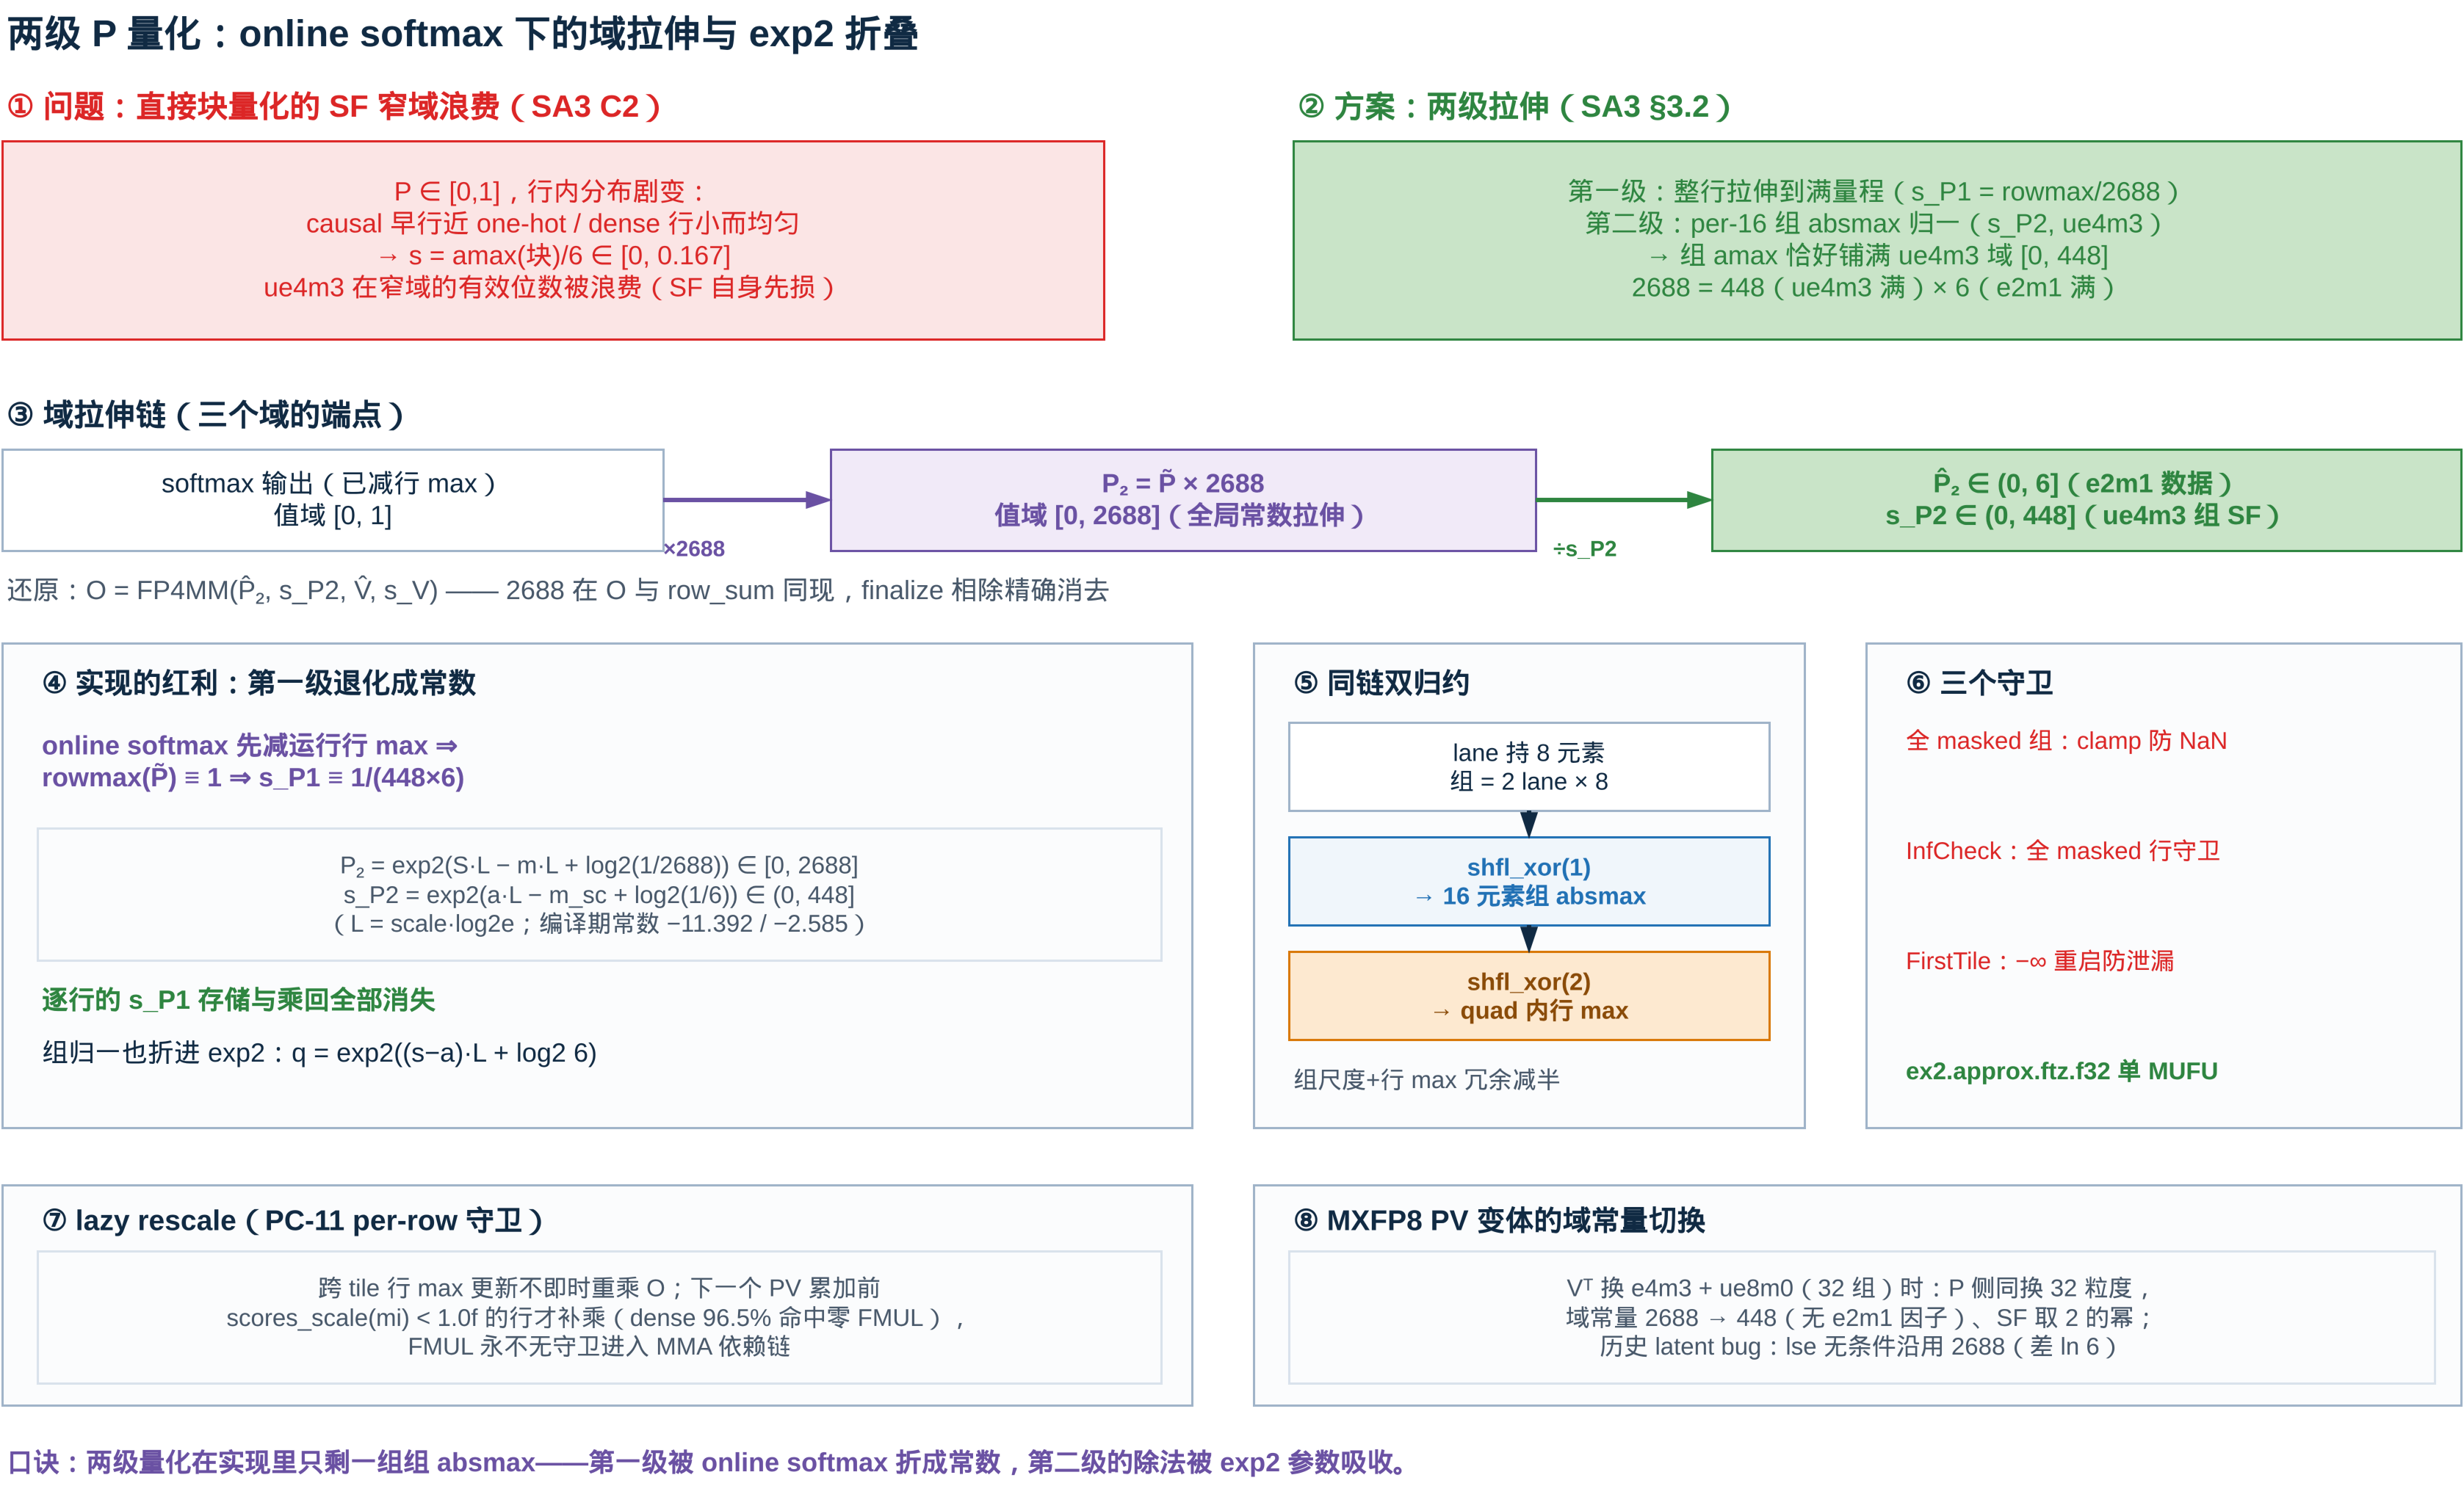
\includegraphics[width=0.98\textwidth]{figures/fig-32-1-two-level-p.png}
  \caption{两级 P 量化的域拉伸：online softmax 使第一级退化为全局常数
  $1/2688$ 并折进 exp2 shift；第二级 per-16 组 absmax 铺满 ue4m3 域，
  组归一化同样折进 exp2 参数。}
\end{figure}

\begin{figure}[H]
  \centering
  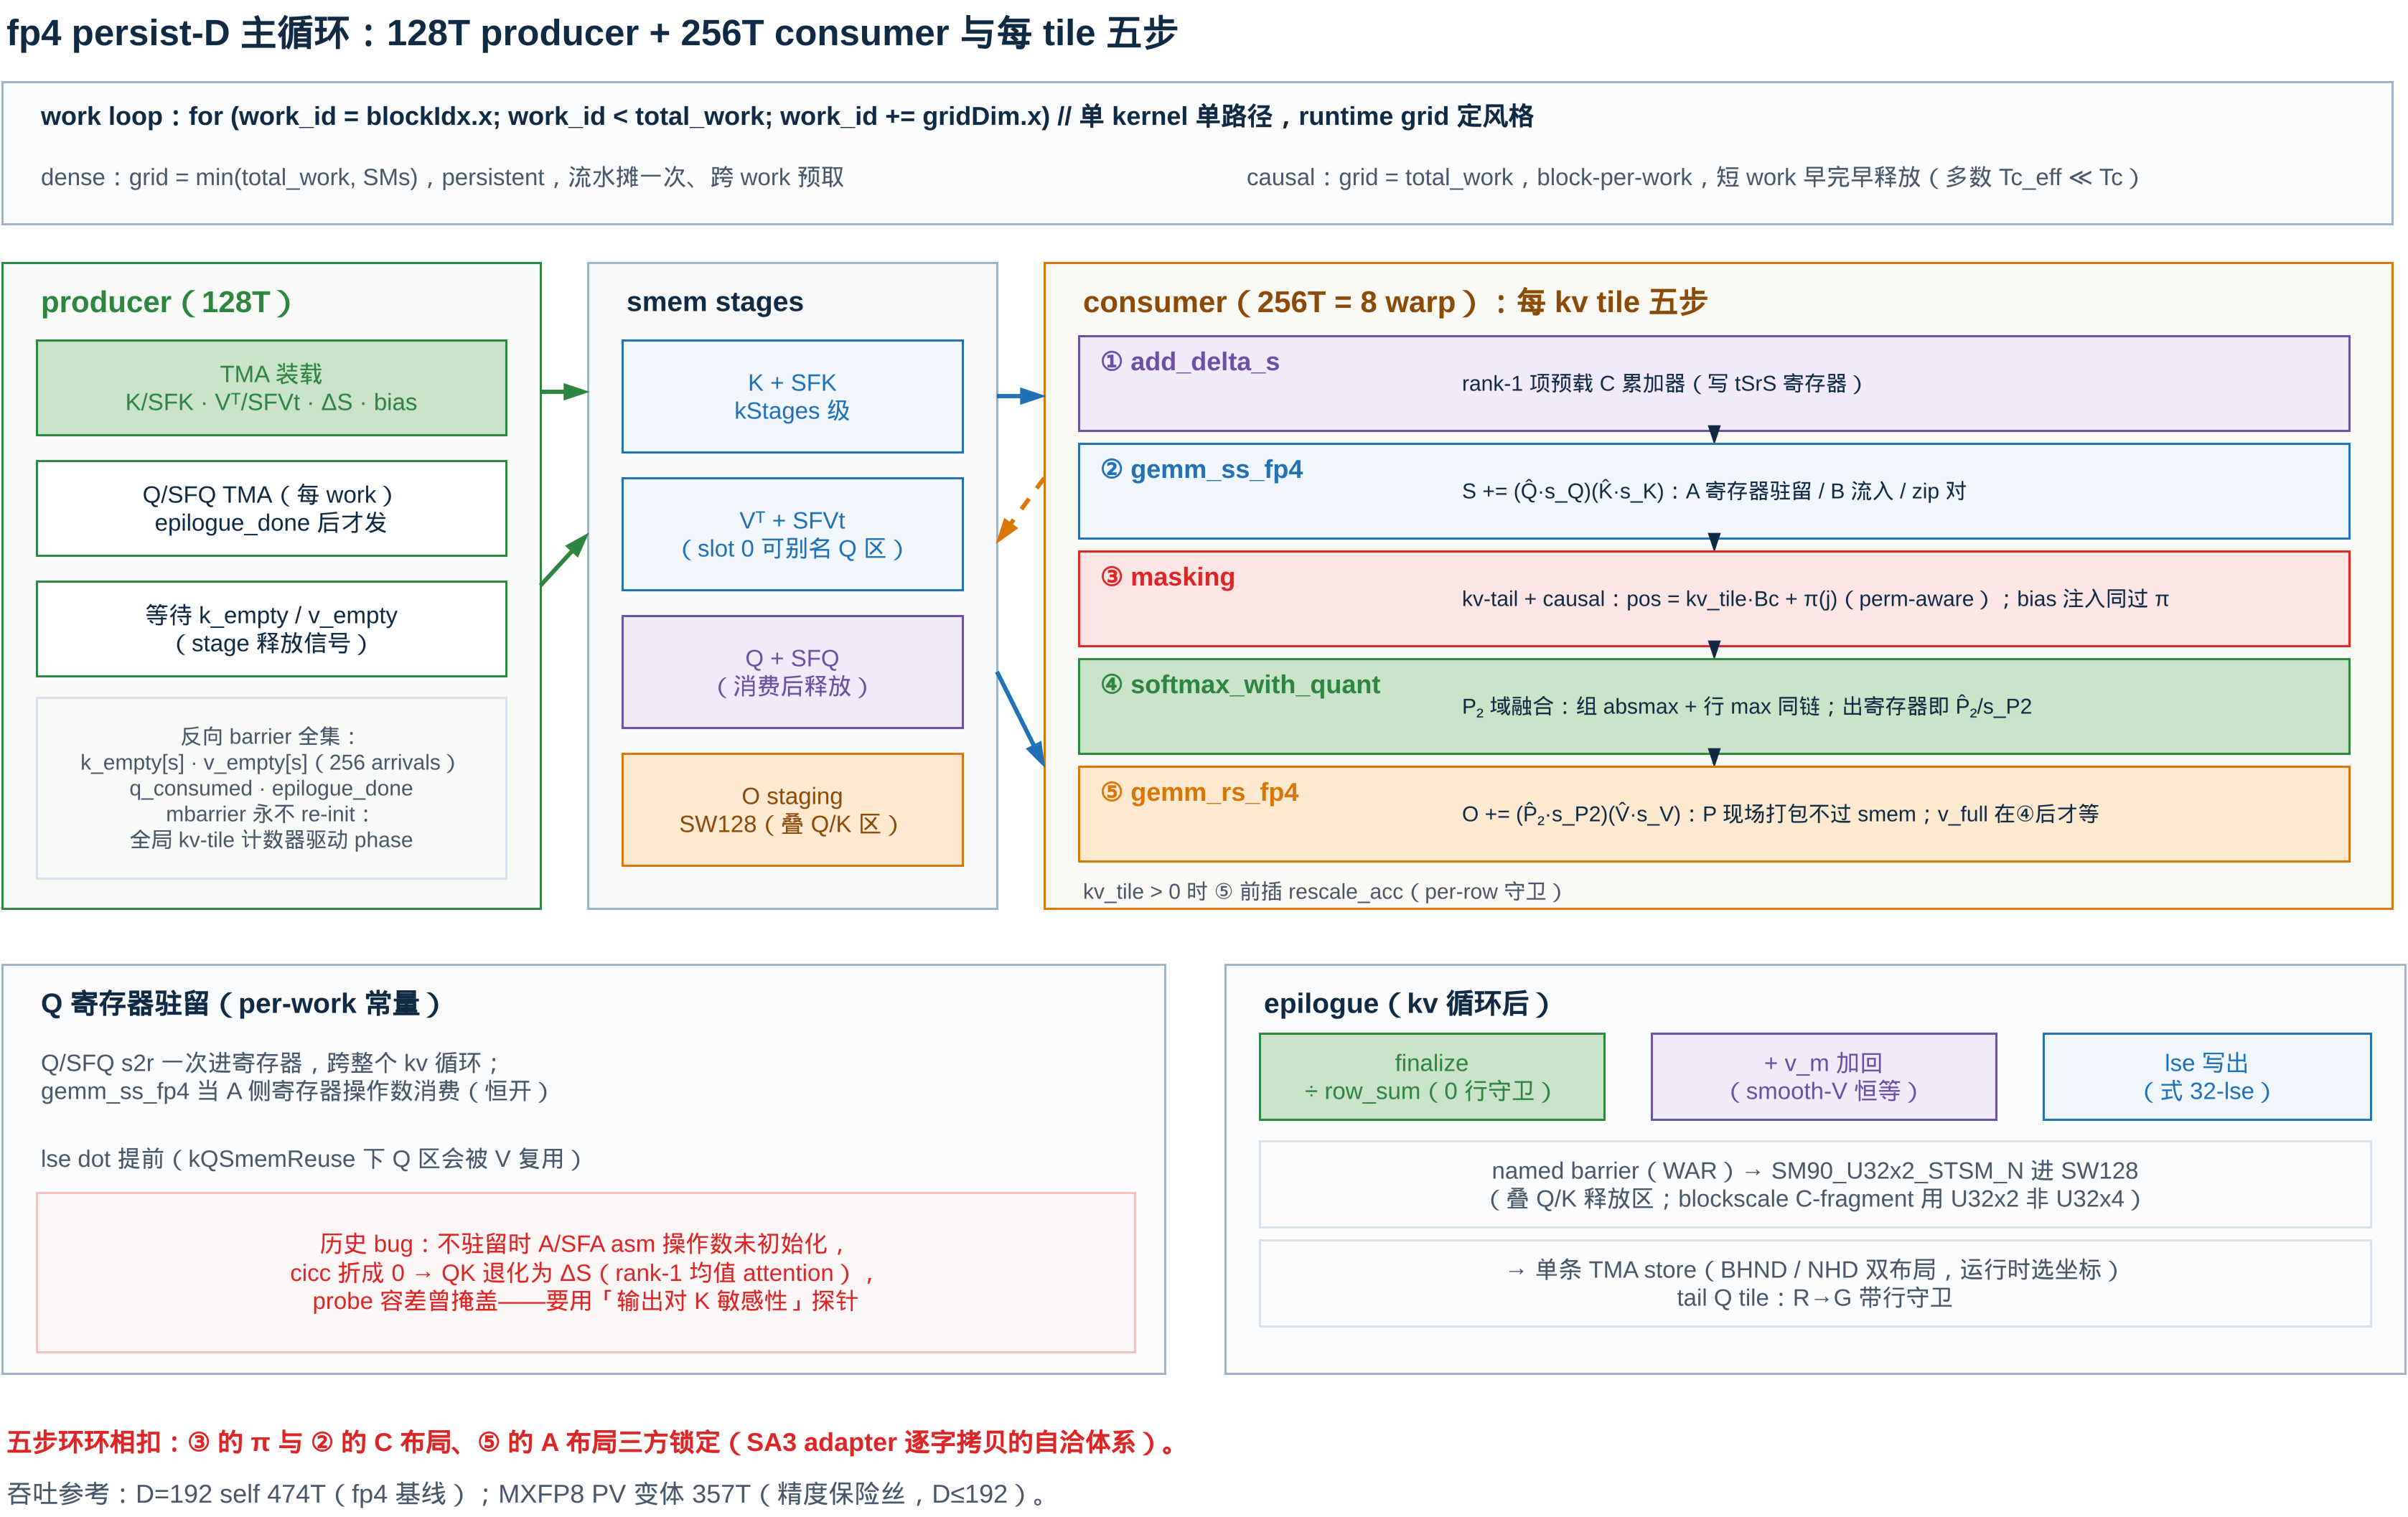
\includegraphics[width=0.98\textwidth]{figures/fig-32-2-persist-d-loop.png}
  \caption{fp4 persist-D 主循环数据流（128T producer + 256T consumer）：
  每 kv tile 的五步（$\Delta S$ 预载 $\to$ QK $\to$ masking $\to$ 融合
  softmax/P 量化 $\to$ PV），barrier 永不 re-init，grid 由 runtime 定
  persistent 或 block-per-work。}
\end{figure}

\section{性能分析}

\subsection{本机 e2e（fp4 vs SDPA）}

表~\ref{tab:32-mxfp8} 汇总 \texttt{--fp4-pv-mm-type fp8} 变体（数据落
盘 \texttt{.tmp/book-bench/ch32/}）；fp4 基线表见
第~\ref{ch:31}~章表 31.2（self 1.49--2.11x、causal 1.23--1.61x，
16 格全绿）。

\begin{table}[H]
  \centering
  \caption{MXFP8 PV 变体 vs fp4 基线（PRO 5000，$B{=}1,H{=}32,N{=}8192$，
  fp16 口径，allclose 全绿）}
  \label{tab:32-mxfp8}
  \begin{tabular}{@{}rlllll@{}}
    \toprule
    $D$ & mxfp8 self (ms) & vs fp4 & mxfp8 causal (ms) & vs fp4 & 加速比
    (self/causal) \\
    \midrule
    64  & 2.24 & $+39\%$ & 1.41 & $+31\%$ & 1.07x / 0.96x \\
    128 & 3.47 & $+38\%$ & 2.17 & $+30\%$ & 1.48x / 1.24x \\
    192 & 4.62 & $+33\%$ & 3.06 & $+28\%$ & 1.56x / 1.25x \\
    \bottomrule
  \end{tabular}
\end{table}

MXFP8 PV 付出 28--39\% 的代价：$V^\top$ 数据 8 bit 带宽翻倍、atom 换
\texttt{m16n8k128}，两者吞吐相近但带宽直接体现在 e2e。它的定位是
\textbf{精度保险丝}（$D\le192$ 的 smem 预算内），不是性能选项
（第~\ref{ch:31}~章 31.6 同结论）。

\subsection{fp4 对 fp8 的相对收益}

历史对照（RFC/skill 记录口径，非本机当日）：attn kernel 本身 fp4 比
fp8 快 $\sim$23\%——blockscale mxf4nvf4 吞吐与 fp8 dense 相当，收益
全部来自\textbf{带宽}（K/V/SF 字节减半以上）；D=192 的 e2e 比值
self 1.47x / causal 1.29x / gqa 1.50x。本机同日对照可复算：fp4
D=192 self 3.48ms（表 31.2）对 fp8 persist-D 同 shape 的表 29.2 数据。

\subsection{已落地与已证伪的微优化}

已落地：条件 rescale（PC-11 per-row 守卫，dense 96.5\% 命中，
-4.9\%；attn-mask 场景再 -3.7/-4.7\%）、\texttt{ex2.approx.ftz.f32}
（消 ptxas range 胶水，-5.9\%）、regalloc 按 D 门控（$D\le128$ 用
\texttt{alloc<224>}，$D\ge192$ 必须 232）。

已证伪（默认关闭/代码保留，勿重复）：Q smem 复用（fp4 的 L1TEX
sector hit 已 96.75\% 饱和，fp8 的前提不成立，实测 +1.8\% 回退，
\texttt{attn\_traits.cuh} L19--28 注释——与 fp8 章的同名机制结论相
反，很好的对照案例）；rescale merge in-place（把 FMUL 拉进 MMA 依赖
链，+1.7\%）；V/SFV 首块 s2r 提前藏进 softmax（PC-4：+1.3--1.7\% 净
负，LDSM 目的寄存器跨 softmax 链拉长 live-range；NCU 证实 B 供给非
瓶颈，wait 主体在 A 操作数串行链——persist-D 微优化到顶的标志）。

\section{实践经验}

\textbf{fragment adapter 是经验锁定的整体}。kv\_perm32、$\Delta S$
槽位算术、\texttt{LayoutP}/\texttt{LayoutSFP} 打包、$V^\top$ 转置存储
——SA3 的这套 adapter 相互补偿、自洽成体系（头注释 L25--37：empirical
lock 在 \texttt{.tmp} 的对齐探针里逐项验证过，dense e2e 与 dequant 仿真
一致）。逐字拷贝 + 只修 masking 是正确的移植姿势；单独「改进」其中
一环会破坏补偿关系。

\textbf{精度评估的口径}。e2m1 的 最坏 $\sim$25\% 的相对量化误差使 P/V 两级误差叠
加后 causal 尖峰行 max\_abs 天然 0.5--0.75（probe 仿真与 kernel 同
级，格式固有）；SA3 论文自身用 cosine 评估。工程验收看 mean\_abs
（0.014--0.03）与容差（dense 0.15 / causal 0.70），用 fp8 的容径卡
fp4 会全军覆没。hybrid（fp16 前 $n_{early}$ 行）是尖峰行的工程解法
（b0/b1 误差 2.6/0.99 $\to$ 0.000/0.001，剩余长尾由 V 量化主导）。

\section{常见坑}

\begin{enumerate}[itemsep=2pt,topsep=2pt]
  \item \textbf{masking 不 perm-aware}：causal 谓词按原始列 index 判
        定，$N{=}512$ max\_abs 3.3（上游 SA3 真实 bug；本章 32.4.3 的
        $pos$ 公式）。
  \item \textbf{mxfp8 域常量}：PV 换 mxfp8 后 lse 仍用 2688——差
        $\ln6$ 的 latent bug，按 \texttt{kPvMxfp8} 编译期分流域常量。
  \item \textbf{mbarrier re-init 是 UB}：跨 work 循环里对活跃 barrier
        re-initialize 行为未定义（PTX ISA 9.7.13.15.9），用全局 tile
        计数器驱动 phase。
  \item \textbf{stale AbsMaxP}：组 absmax 寄存器跨 tile/跨 work 复用，
        每 FirstTile 必须从 $-\infty$ 重新起步（L151--154 注释），
        否则上个 work 的尺度泄漏进当前行。
  \item \textbf{未初始化 asm 操作数被折叠}：Q 不驻留寄存器时 cicc 把
        A/SFA 操作数折成 0，QK 静默退化（32.4.2 的历史 bug）。
  \item \textbf{subbyte smem 指针}：e2m1 tensor 必须
        \texttt{make\_smem\_ptr}，裸 \texttt{reinterpret\_cast} 地址差
        2 倍、stage$\ge$1 TMA 越界（第~\ref{ch:31}~章 31.4.6）。
\end{enumerate}

\section{面试要点速查}

\begin{enumerate}[itemsep=2pt,topsep=2pt]
  \item 两级 P 量化：$s_{P1}=\mathrm{rowmax}/2688$、
        $\tilde P_2\in[0,2688]$、$s_{P2}$ per-16 组 ue4m3；2688 =
        448（ue4m3 满）$\times$ 6（e2m1 满）。
  \item online softmax 的退化红利：行 max 恒 1 $\Rightarrow$ 第一级变
        全局常数折进 exp2 shift——两级量化在实现里只剩一组 absmax。
  \item 组归一化折进 exp2 参数：$q=\exp_2((s-a)L+\log_2 6)$，rcp 与
        FMUL 段消失；row\_sum 用 FMA 吸收 $s_{P2}$。
  \item 2688 的消去：$O$ 与 row\_sum 同带常数，finalize 相除精确抵消。
  \item dense persistent / causal block-per-work：单 kernel 单路径，
        runtime grid 定风格；barrier phase 由全局 tile 计数器驱动。
  \item blockscale QK/PV 的 A 侧差异：Q 寄存器驻留（per-work 常量）、
        P 寄存器现场打包（quantize\_and\_pack\_p），B 侧才走 smem
        stage。
  \item fp4 vs fp8 的收益来源：MMA 吞吐持平、带宽减半——memory-bound
        attention 的收益逻辑。
\end{enumerate}

\section{最小测试与动手实验}

\begin{lstlisting}[style=console]
export CUDA_VISIBLE_DEVICES=7 FFPA_CUDA_ALLOW_SMALL_D=1
python -m ffpa_attn.bench --fwd-backend cuda --cuda-impl fp4 \
  --tasks self-attn causal --D 192 --no-bwd --show-allclose
# MXFP8 PV（精度保险丝，D<=192）：
python -m ffpa_attn.bench --fwd-backend cuda --cuda-impl fp4 \
  --tasks self-attn causal --D 192 --no-bwd --show-allclose \
  --fp4-pv-mm-type fp8
\end{lstlisting}

\begin{enumerate}[itemsep=2pt,topsep=2pt]
  \item \textbf{两级域验证}：读 \texttt{fp4\_pscale.cuh} L117--128 的
        三个编译期常数，手推
        式~\ref{eq:32-p2-domain} 的两个值域端点（$P_2=2688$ 当
        $s=m$；$s_{P2}=448$ 当组 absmax $=$ 行 max）。
  \item \textbf{mxfp8 A/B}：复现表~\ref{tab:32-mxfp8} 的三档 D，验证
        $D{=}256$ 被 traits 的 smem 断言拒绝。
  \item \textbf{causal 风格对照}：读 \texttt{launch/cute\_fp4\_persist\_d.cuh} 的
        grid 选择（\texttt{causal ? total\_work : min(...)}），解释为
        什么 causal 的多数 work 选 block-per-work。
  \item \textbf{InfCheck 场景}：构造 $N_q>N_{kv}$ 的 cross 输入跑
        causal，确认左上角全 masked 行的 lse/O 有限（无 NaN）。
\end{enumerate}

\section*{延伸阅读}
\addcontentsline{toc}{section}{延伸阅读}

\begin{itemize}[itemsep=0pt,topsep=2pt]
  \item \texttt{cute/fp4/sm\_120/persist\_d.cuh} 头注释（L1--55）：
        数学链、列对齐锁定、两级 P、subbyte；
  \item \texttt{cute/fp4/fp4\_pscale.cuh} L117--195：融合 softmax 的
        域折叠与 shuffle 链；
  \item \texttt{cute/fp4/fp4\_gemm.cuh} L91--218：\texttt{gemm\_ss\_fp4}
        与 \texttt{gemm\_rs\_fp4} 的流水与 barrier 协议；
  \item SageAttention3 论文 §3.2（两级量化）与 Algorithm 1（完整数值
        链）；sm\_120 split-D 与 M4N2 家族见第~\ref{ch:30}~章的 fp8
        同构实现。
\end{itemize}

% ch33-fp8-fp4-bench.tex — FP8/FP4 性能实战：bench、精度与生态（RFC-K7）
% 源码：ffpa-attn(861d75e) bench/bench_fp8.py(719L) + bench/bench_fp4.py(652L) + ffpa_attn.bench CLI
\chapter{FP8/FP4 性能实战：Bench、精度与生态}\label{ch:33}

\section{本章导读}
% 前置：\ref{ch:29}/\ref{ch:30}/\ref{ch:32}

\section{问题与动机}
% 如何科学度量量化 attention：speedup 口径、精度口径、E2E 占比

\section{数学原理}
% speedup = (T_self + d_SDPA)/(T_self + d_FFPA)；精度评估口径（max_abs tol / cosine / mean_abs）

\section{设计与实现}
% ffpa_attn.bench CLI 全 knob 矩阵（--cuda-impl fp8/fp4 家族、quant method、acc type、hybrid）；
% bench/bench_fp8.py、bench_fp4.py 的 D/N 扫描与 plot 输出

\section{图示}
% README 5090 speedup 图引用（fp8 D64-768 / fp4 D64-512）+ 本机 PRO 5000 复测 plot

\section{性能分析}
% 本机复测 vs README 5090；aux 链 E2E 占比；kernel tensor pipe 77%；
% knob 矩阵实测表（QK int8/fp8 x PV f16/f32 x per-block/thread x hybrid）

\section{实践经验}

\section{常见坑}
% A/B 必须校验 SDPA 参照一致性；配置必须显式声明（默认已统一 int8+f16acc）

\section{面试要点速查}

\section{最小测试与动手实验}
% 完整 task 矩阵（self/causal/gqa/cross x D{64..512}）+ knob 实验 + plot 落盘


\appendix
% appA-common-toolbox.tex — 骨架（RFC-0.3）
\chapter{附录 A\quad 基础设施工具箱：common.cuh 解析}\label{app:A}

本章待撰写。MMA/WGMMA PTX 宏、swizzle v1/v2、TMA/mbarrier helpers、TensorMap、setmaxnreg（I.1）。

% appB-perf-data.tex — 骨架（RFC-0.3）
\chapter{附录 B\quad 性能数据与口径}\label{app:B}

本章待撰写。README SM120a 表 + 对应章节/函数名列 + 复测数据（RFC-G 合入，I.2）。

% appC-build-guide.tex — 骨架（RFC-0.3）
\chapter{附录 C\quad 构建、运行与最小测试指南}\label{app:C}

本章待撰写。build.sh、章 $\times$ 编译宏 $\times$ arch 矩阵、环境安装、notes-v2.cu 角色声明（I.3）。

% appD-source-index.tex — 附录 D 源码索引 v1（RFC-A.5）
% permalink 基准 commit：6cd32de（tag v4.0.0，2026-09-17；anchors.yaml repo_commit）
\chapter{源码索引}\label{app:D}

正文关键代码段的完整实现入口。行区间与 \texttt{scripts/\allowbreak{}anchors.\allowbreak{}yaml} 冻结登记一致；
链接为 GitHub commit permalink（防 branch 漂移）。

\begin{longtable}{llp{7.2cm}}
\toprule
章 & 主题 & 源码区间（permalink） \\
\midrule
\endfirsthead
\toprule
章 & 主题 & 源码区间（permalink） \\
\midrule
\endhead
A & common.cuh 工具箱 & \href{https://github.com/xlite-dev/LeetCUDA/blob/6cd32deca683d6c4aae2011988c9f4a35bc5f528/kernels/interview/common.cuh#L1-L803}{common.cuh L1--L803} \\
第01 & GPU 架构/Roofline 速查 & \href{https://github.com/xlite-dev/LeetCUDA/blob/6cd32deca683d6c4aae2011988c9f4a35bc5f528/kernels/interview/base.cuh#L1-L86}{base.cuh L1--L86} \\
第02 & warp/block 归约与 dot & \href{https://github.com/xlite-dev/LeetCUDA/blob/6cd32deca683d6c4aae2011988c9f4a35bc5f528/kernels/interview/base.cuh#L87-L305}{base.cuh L87--L305} \\
第03 & 向量化与原子操作 & \href{https://github.com/xlite-dev/LeetCUDA/blob/6cd32deca683d6c4aae2011988c9f4a35bc5f528/kernels/interview/base.cuh#L306-L386}{base.cuh L306--L386} \\
第04 & softmax 三级递进 & \href{https://github.com/xlite-dev/LeetCUDA/blob/6cd32deca683d6c4aae2011988c9f4a35bc5f528/kernels/interview/base.cuh#L520-L665}{base.cuh L520--L665} \\
第05 & merge\_attn\_states & \href{https://github.com/xlite-dev/LeetCUDA/blob/6cd32deca683d6c4aae2011988c9f4a35bc5f528/kernels/interview/base.cuh#L387-L519}{base.cuh L387--L519} \\
第06 & RMSNorm/LayerNorm & \href{https://github.com/xlite-dev/LeetCUDA/blob/6cd32deca683d6c4aae2011988c9f4a35bc5f528/kernels/interview/base.cuh#L666-L801}{base.cuh L666--L801} \\
第07 & RoPE 与转置 & \href{https://github.com/xlite-dev/LeetCUDA/blob/6cd32deca683d6c4aae2011988c9f4a35bc5f528/kernels/interview/base.cuh#L802-L909}{base.cuh L802--L909} \\
第08 & sgemv 三种划分 & \href{https://github.com/xlite-dev/LeetCUDA/blob/6cd32deca683d6c4aae2011988c9f4a35bc5f528/kernels/interview/sgemv.cuh#L1-L102}{sgemv.cuh L1--L102} \\
第09 & sgemm 阶梯一 & \href{https://github.com/xlite-dev/LeetCUDA/blob/6cd32deca683d6c4aae2011988c9f4a35bc5f528/kernels/interview/sgemm.cuh#L6-L183}{sgemm.cuh L6--L183} \\
第10 & sgemm TF32/WMMA & \href{https://github.com/xlite-dev/LeetCUDA/blob/6cd32deca683d6c4aae2011988c9f4a35bc5f528/kernels/interview/sgemm.cuh#L184-L434}{sgemm.cuh L184--L434} \\
第11 & hgemm mma.sync & \href{https://github.com/xlite-dev/LeetCUDA/blob/6cd32deca683d6c4aae2011988c9f4a35bc5f528/kernels/interview/hgemm.cuh#L3-L397}{hgemm.cuh L3--L397} \\
第12 & hgemm swizzle & \href{https://github.com/xlite-dev/LeetCUDA/blob/6cd32deca683d6c4aae2011988c9f4a35bc5f528/kernels/interview/hgemm.cuh#L399-L716}{hgemm.cuh L399--L716}, \href{https://github.com/xlite-dev/LeetCUDA/blob/6cd32deca683d6c4aae2011988c9f4a35bc5f528/kernels/interview/common.cuh#L110-L348}{common.cuh L110--L348} \\
第13 & WGMMA/TMA/mbarrier & \href{https://github.com/xlite-dev/LeetCUDA/blob/6cd32deca683d6c4aae2011988c9f4a35bc5f528/kernels/interview/hgemm.cuh#L1428-L1857}{hgemm.cuh L1428--L1857}, \href{https://github.com/xlite-dev/LeetCUDA/blob/6cd32deca683d6c4aae2011988c9f4a35bc5f528/kernels/interview/common.cuh#L350-L803}{common.cuh L350--L803} \\
第14 & SM120 TMA+WS & \href{https://github.com/xlite-dev/LeetCUDA/blob/6cd32deca683d6c4aae2011988c9f4a35bc5f528/kernels/interview/hgemm.cuh#L1859-L2100}{hgemm.cuh L1859--L2100}, \href{https://github.com/xlite-dev/LeetCUDA/blob/6cd32deca683d6c4aae2011988c9f4a35bc5f528/kernels/interview/common.cuh#L462-L475}{common.cuh L462--L475} \\
第15 & FA 原理（头注释） & \href{https://github.com/xlite-dev/LeetCUDA/blob/6cd32deca683d6c4aae2011988c9f4a35bc5f528/kernels/interview/flash_attn.cuh#L5-L110}{flash\_attn.cuh L5--L110} \\
第16 & FA2 split-Q+MMA & \href{https://github.com/xlite-dev/LeetCUDA/blob/6cd32deca683d6c4aae2011988c9f4a35bc5f528/kernels/interview/flash_attn.cuh#L5-L790}{flash\_attn.cuh L5--L790} \\
第17 & FA2 TMA+WS & \href{https://github.com/xlite-dev/LeetCUDA/blob/6cd32deca683d6c4aae2011988c9f4a35bc5f528/kernels/interview/flash_attn.cuh#L792-L1440}{flash\_attn.cuh L792--L1440} \\
第18 & FA3 双 consumer & \href{https://github.com/xlite-dev/LeetCUDA/blob/6cd32deca683d6c4aae2011988c9f4a35bc5f528/kernels/interview/flash_attn.cuh#L1441-L2192}{flash\_attn.cuh L1441--L2192} \\
第19 & FFPA split-D 全篇 & \href{https://github.com/xlite-dev/LeetCUDA/blob/6cd32deca683d6c4aae2011988c9f4a35bc5f528/kernels/interview/ffpa_attn.cuh#L1-L641}{ffpa\_attn.cuh L1--L641} \\
第20 & CuTe Layout 对照 & \href{https://github.com/xlite-dev/LeetCUDA/blob/6cd32deca683d6c4aae2011988c9f4a35bc5f528/kernels/interview/hgemm.cuh#L788-L820}{hgemm.cuh L788--L820} \\
第21 & CuTe TiledCopy 对照 & \href{https://github.com/xlite-dev/LeetCUDA/blob/6cd32deca683d6c4aae2011988c9f4a35bc5f528/kernels/interview/hgemm.cuh#L821-L1196}{hgemm.cuh L821--L1196} \\
第22 & CuTe TiledMMA 对照 & \href{https://github.com/xlite-dev/LeetCUDA/blob/6cd32deca683d6c4aae2011988c9f4a35bc5f528/kernels/interview/ffpa_attn.cuh#L31-L79}{ffpa\_attn.cuh L31--L79} \\
第23 & CuTe SW128 atom 对照 & \href{https://github.com/xlite-dev/LeetCUDA/blob/6cd32deca683d6c4aae2011988c9f4a35bc5f528/kernels/interview/hgemm.cuh#L1232-L1270}{hgemm.cuh L1232--L1270} \\
第24 & CuTe HGEMM & \href{https://github.com/xlite-dev/LeetCUDA/blob/6cd32deca683d6c4aae2011988c9f4a35bc5f528/kernels/interview/hgemm.cuh#L718-L1427}{hgemm.cuh L718--L1427} \\
第25 & CuTe FA 三实现 & \href{https://github.com/xlite-dev/LeetCUDA/blob/6cd32deca683d6c4aae2011988c9f4a35bc5f528/kernels/interview/flash_attn.cuh#L2196-L3488}{flash\_attn.cuh L2196--L3488} \\
第26 & CuTe FFPA 双 TiledMMA & \href{https://github.com/xlite-dev/LeetCUDA/blob/6cd32deca683d6c4aae2011988c9f4a35bc5f528/kernels/interview/ffpa_attn.cuh#L30-L65}{ffpa\_attn.cuh L30--L65}, \href{https://github.com/xlite-dev/LeetCUDA/blob/6cd32deca683d6c4aae2011988c9f4a35bc5f528/kernels/interview/ffpa_attn.cuh#L79-L375}{ffpa\_attn.cuh L79--L375}, \href{https://github.com/xlite-dev/LeetCUDA/blob/6cd32deca683d6c4aae2011988c9f4a35bc5f528/kernels/interview/ffpa_attn.cuh#L377-L640}{ffpa\_attn.cuh L377--L640} \\
\multicolumn{3}{l}{\footnotesize 增补章（ch26b/ch26c/ch34/ch35）源码为本仓新增/追加区间（ffpa\_attn.cuh L643--L1306、} \\
\multicolumn{3}{l}{\footnotesize fp8\_gemm.cuh L1--L958、notes-v2.cu 集成 harness），随增补 commit 在 anchors.yaml 冻结} \\
\multicolumn{3}{l}{\footnotesize 以下 Part VI（第27--33 章）源码在 \texttt{ffpa-attn} 仓（commit \texttt{861d75e}），路径前缀以 \texttt{csrc/cuffpa/} 为主（bench 与 CLI 见第33章）} \\
第27 & 量化注意力数学 & \href{https://github.com/xlite-dev/ffpa-attn/blob/861d75ee87824a14a9ebfe295d54c7dac3e3cabc/csrc/cuffpa/cute/fp8/fp8_pscale.cuh#L17-L37}{cute/fp8/fp8\_pscale.cuh L17--L37}, \href{https://github.com/xlite-dev/ffpa-attn/blob/861d75ee87824a14a9ebfe295d54c7dac3e3cabc/csrc/cuffpa/cute/fp8/fp8_pscale.cuh#L111-L138}{L111--L138} \\
第28 & fp8 量化前处理链 & \href{https://github.com/xlite-dev/ffpa-attn/blob/861d75ee87824a14a9ebfe295d54c7dac3e3cabc/csrc/cuffpa/cute/fp8/smooth_k.cuh#L12-L84}{cute/fp8/smooth\_k.cuh L12--L84}, \href{https://github.com/xlite-dev/ffpa-attn/blob/861d75ee87824a14a9ebfe295d54c7dac3e3cabc/csrc/cuffpa/cute/fp8/quantize_fp8.cuh#L29-L201}{cute/fp8/quantize\_fp8.cuh L29--L201}, \href{https://github.com/xlite-dev/ffpa-attn/blob/861d75ee87824a14a9ebfe295d54c7dac3e3cabc/csrc/cuffpa/cute/hadamard.cuh#L1-L92}{cute/hadamard.cuh L1--L92} \\
第29 & fp8 persist-D & \href{https://github.com/xlite-dev/ffpa-attn/blob/861d75ee87824a14a9ebfe295d54c7dac3e3cabc/csrc/cuffpa/cute/fp8/sm_120/persist_d.cuh#L37-L215}{cute/fp8/sm\_120/persist\_d.cuh L37--L215}, \href{https://github.com/xlite-dev/ffpa-attn/blob/861d75ee87824a14a9ebfe295d54c7dac3e3cabc/csrc/cuffpa/cute/fp8/sm_120/persist_d.cuh#L583-L1031}{L583--L1031}, \href{https://github.com/xlite-dev/ffpa-attn/blob/861d75ee87824a14a9ebfe295d54c7dac3e3cabc/csrc/cuffpa/cute/fp8/reg2reg_8b.cuh#L14-L141}{cute/fp8/reg2reg\_8b.cuh L14--L141} \\
第30 & fp8 split-D/M4N2 & \href{https://github.com/xlite-dev/ffpa-attn/blob/861d75ee87824a14a9ebfe295d54c7dac3e3cabc/csrc/cuffpa/cute/fp8/sm_120/split_d.cuh#L39-L245}{cute/fp8/sm\_120/split\_d.cuh L39--L245}, \href{https://github.com/xlite-dev/ffpa-attn/blob/861d75ee87824a14a9ebfe295d54c7dac3e3cabc/csrc/cuffpa/cute/fp8/sm_120/split_d.cuh#L446-L756}{L446--L756}, \href{https://github.com/xlite-dev/ffpa-attn/blob/861d75ee87824a14a9ebfe295d54c7dac3e3cabc/csrc/cuffpa/cute/fp8/sm_120/split_d_m4n2.cuh#L300-L970}{split\_d\_m4n2.cuh L300--L970} \\
第31 & fp4 量化链 & \href{https://github.com/xlite-dev/ffpa-attn/blob/861d75ee87824a14a9ebfe295d54c7dac3e3cabc/csrc/cuffpa/cute/fp4/quantize_fp4.cuh#L32-L320}{cute/fp4/quantize\_fp4.cuh L32--L320}, \href{https://github.com/xlite-dev/ffpa-attn/blob/861d75ee87824a14a9ebfe295d54c7dac3e3cabc/csrc/cuffpa/cute/fp4/quantize_fp4.cuh#L322-L496}{L322--L496}, \href{https://github.com/xlite-dev/ffpa-attn/blob/861d75ee87824a14a9ebfe295d54c7dac3e3cabc/csrc/cuffpa/cute/fp4/delta_s.cuh#L2-L161}{cute/fp4/delta\_s.cuh L2--L161} \\
第32 & fp4 persist-D & \href{https://github.com/xlite-dev/ffpa-attn/blob/861d75ee87824a14a9ebfe295d54c7dac3e3cabc/csrc/cuffpa/cute/fp4/sm_120/persist_d.cuh#L1-L120}{cute/fp4/sm\_120/persist\_d.cuh L1--L120}, \href{https://github.com/xlite-dev/ffpa-attn/blob/861d75ee87824a14a9ebfe295d54c7dac3e3cabc/csrc/cuffpa/cute/fp4/sm_120/persist_d.cuh#L722-L1066}{L722--L1066}, \href{https://github.com/xlite-dev/ffpa-attn/blob/861d75ee87824a14a9ebfe295d54c7dac3e3cabc/csrc/cuffpa/cute/fp4/fp4_pscale.cuh#L117-L346}{cute/fp4/fp4\_pscale.cuh L117--L346} \\
第33 & bench 与 CLI & \href{https://github.com/xlite-dev/ffpa-attn/blob/861d75ee87824a14a9ebfe295d54c7dac3e3cabc/bench/bench_fp8.py#L1-L140}{bench/bench\_fp8.py L1--L140}, \href{https://github.com/xlite-dev/ffpa-attn/blob/861d75ee87824a14a9ebfe295d54c7dac3e3cabc/src/ffpa_attn/cli/_bench.py#L347-L490}{src/ffpa\_attn/cli/\_bench.py L347--L490} \\
\bottomrule
\end{longtable}

基准 commit：LeetCUDA \texttt{6cd32de}（v4.0.0，2026-09-17 冻结）；
Part VI 各章 ffpa-attn \texttt{861d75e}（2026-09-16 锚定）；Part V 两章
（第~\ref{ch:34}、\ref{ch:35}）与增补章（ch26b/ch26c）为本仓新增区间，
随增补 commit 在 \texttt{anchors.yaml} 冻结。行号漂移由
\texttt{verify\_\allowbreak{}anchors.\allowbreak{}py} 兜底：SHA256 + 首末行锚点双重校验。

% appE-references.tex — 骨架（RFC-0.3）
\chapter{附录 E\quad 参考资料全集}\label{app:E}

本章待撰写。知乎作者/文章/链接/对应章节/引用日期/图片引用清单（RFC-B 合入，I.5）。


\backmatter
\end{document}
